%&header
%
%\newif\ifPhdDoc\PhdDoctrue
\newif\ifMonolithic\Monolithictrue
%\newif\ifTODO\TODOtrue                        % Use todo notes?

\newif\ifRootBuild\RootBuildfalse
\newif\ifOverLeaf\OverLeaffalse
\newif\ifIncludeWritingTips\IncludeWritingTipstrue


\documentclass[
uiophd
, 12pt
, english
, floatrow
%  , xelatex
, glossary                                     % Use a glossary
, biblatex                                 % Use a bibliography
%  , draft
%  , layout
, todos
]{common/mytemplate}
 

%\typeout{++++standalone++++}
%\usepackage[subpreambles=true]{standalone}

% \typeout{++++import++++}
% \usepackage{import}

% \typeout{--------------}
%\hypersetup{
%   bookmarksopen=true
% , bookmarksopenlevel=2
%}

\newcommand*\cleartoleftpage{%
	\clearpage
	\ifodd\value{page}\hbox{}\newpage\fi
}
% Fonts:
% https://tex.stackexchange.com/questions/19898/getting-urw-garamond-and-the-license

\providecommand*\paper[1]{}
\renewcommand*\paper[1]{{\bf{}Paper #1}}

\providecommand\1{}
\renewcommand*\1{\vec 1}
\providecommand\a{}
\renewcommand*\a{\vec a}
\providecommand\b{}
\renewcommand*\b{\vec b}
\providecommand\eR{}
\renewcommand*\eR{\mat{\hat R}}
\providecommand\eRi{}
\renewcommand*\eRi{\hat{\mat R}\;\!^{-1}}
\providecommand\k{}
\renewcommand*\k{\vec k}
\providecommand\n{}
\renewcommand*\n{\vec n}
\providecommand\p{}
\renewcommand*\p{\vec p}
\providecommand\R{}
\renewcommand*\R{\mat R}
\providecommand\Ri{}
\renewcommand*\Ri{\R^{-1}}
\providecommand\s{}
\renewcommand*\s{\vec s}

\providecommand\v{}
\renewcommand*\v{\vec v}
\providecommand\x{}
\renewcommand*\x{\vec x}
\providecommand\X{}
\renewcommand*\X{\mat X}
\providecommand\w{}
\renewcommand*\w{\vec w}

\providecommand\argmin{}
\renewcommand*\argmin[1]{\underset{#1}{\text{argmin}}\ }
\providecommand\norm{}
\renewcommand*\norm[1]{\left\lVert #1 \right\rVert}
\providecommand\min{}
\renewcommand*\min[1]{\underset{#1}{\text{min}}}
\providecommand\sinc{}
\renewcommand\sinc{\text{sinc}}

\providecommand*\nn{}
\renewcommand*\nn{\nonumber\\}

\providecommand\sumb{}
\renewcommand\sumb[2]{\sum\limits_{#1}^{#2}\;}

% \typeout{++++mylatexformat++++}
% \usepackage{mylatexformat}
\typeout{++++floatrow++++}
\usepackage{floatrow}
%\usepackage{bibtex}
%\usepackage{comment}
\typeout{++++environ++++}
\usepackage{environ}
%\usepackage[runin]{abstract}
\typeout{++++parskip++++}
\usepackage[parfill]{parskip}
\typeout{++++glossaries++++}
\usepackage[nonumberlist,nogroupskip]{glossaries}
\typeout{++++afterpage++++}
\usepackage{afterpage}
% \typeout{++++placeins++++}
% \usepackage{afterpage}
\typeout{++++subfiles++++}
\usepackage{subfiles}
%\typeout{++++standalone++++}
%\usepackage{standalone}
\typeout{++++subfig++++}
\usepackage[caption=false,font=footnotesize]{subfig}
\typeout{--------------}


% \newcommand\gls[1]{#1}

\renewcommand\figurename{Fig.}
\renewcommand\thefigure{\arabic{figure}}
\usepackage[margin=0pt,font={it,small},labelfont={bf,it},labelsep=colon]{caption}
% \addto\captionsenglish{\renewcommand{\figurename}{Fig.}}

\renewcommand\thetable{\arabic{table}} 
\renewcommand\theequation{\arabic{equation}} 

% Increase header a bit to allow two lines in it
\addtolength\headheight{\topmargin}
\setlength\topmargin{0pt}

\titleformat{\chapter}%command
[display]%shape
% {}%format
{\flushright}%format
{}%label
{0pt}%sep
{\color{Black}\bfseries\Huge}%before
[]%after
\titlespacing*{\chapter}{0pt}{*0}{*2}

\titleformat{\section}%command
[block]%shape
% {}%format
{\Large\bfseries}%format
{\thesection}%label
{10pt}%sep
{}%before
[]%after
\titlespacing*{\section}{0pt}{*0}{*0}

\titleformat{\subsection}%command
[block]%shape
% {}%format
{\large\bfseries}%format
{\thesubsection}%label
{10pt}%sep
{}%before
[]%after
\titlespacing*{\subsection}{0pt}{*0}{*0}

\addbibresource{../library.bib}
%\ifMonolithic
%\addbibresource{../HowtoHowtoCapon/library.bib}
%\fi

\renewcommand\include[1]{\subfile{#1}}

\vbadness=99999
\hbadness=99999

\endofdump
\begin{document}
	
\end{document}


%
%
% COMPILATION REQUIREMENTS
%
% http://tug.org/fonts/getnonfreefonts/

\endofdump

\RootBuildtrue

\title{Swift, Smart, Supreme - Sonar cognition with adaptive image reconstruction and synthesis}

%\title{Faster, Smarter, Better - Adaptive sonars powered by graphics processing units}
%\title{Faster, Smarter, Better - Smart sonars powered by  systems of tomorrow Powering sonar systems with intelligence using adaptive beamforming and performance computing and adaptive image reconstruction to create cognitive sonar systems of tomorrow}
\author{Jo Inge Buskenes}
%\department{Department of Informatics}


%\setlength\parskip{\baselineskip}

%\setlength\parindent{0pt}                       %Indent first line in each paragraph?
%\setlength\parskip{1cm%                         % baseskip
%	plus.5\baselineskip%          % amount of stretch
%	minus.3\baselineskip}          % pickyness on underfull vbox

%\includepackage{subfiles}

\newglossaryentry{ASIC}{name={ASIC},
                  description={Application Specific Integrated Circuit} } 
                  
\newglossaryentry{ATR}{name={ATR},
                  description={Automatic Target Recognition} } 

\newglossaryentry{CPU}{name={CPU},
						description={Central Processing Unit} } 

\newglossaryentry{GPGPU}{name={GPGPU},
						description={General Purpose Graphics Processing Unit} } 

\newglossaryentry{GPU}{name={GPU},
						description={Graphics Processing Unit} } 
					
\newglossaryentry{MVDR}{name={MVDR},
						description={Minimum Variance Distortionless Response} } 
\makeglossaries

\addbibresource{../library.bib}






%% This is mostly ripped from the 'quotchap' package. It did not perform to my liking, so I've
%% tweaked it some... 
%
%
%% charter         bch
%% palatino        ppl
%% avantgarde      pag
%% bookman         pbk
%% courier         pcr
%% helvetica       phv
%% newcentury      pnc
%% times           ptm
%% utopia          put
%
% \def\@defaultcnfont{ptm}
% 
%% \newif\if@usecolor\@usecolortrue
% \newcommand*{\@newfontcmd}{\@ifundefined{@defaultcnfont}{\newcommand*}{%
%     \PackageWarning{quotchap}{%
%       You have tried to specify more than one font to be\MessageBreak
%       used for the chapter numbers. I ignore the font\MessageBreak
%       `\CurrentOption'}
%     \providecommand*}}
% 
% % \DeclareOption{grey}{\@usecolortrue}
% % \DeclareOption{nogrey}{\@usecolorfalse}
% \providecommand*{\@defaultcnfont}{pbk}
%% \if@usecolor
%   \definecolor{chaptergrey}{rgb}{0.6,0.6,0.6}%
%% \else
%%   \providecommand*{\color}[1]{}
%% \fi
% 
% \newcommand*{\chapnumfont}{%
%   \usefont{T1}{\@defaultcnfont}{b}{n}\fontsize{100}{130}\selectfont%
%   \color{TealBlue}}
% \let\size@chapter\huge
% \providecommand*{\chapterheadstartvskip}{\vspace*{2.3\baselineskip}}
% \providecommand*{\chapterheadendvskip}{\vspace{1.7\baselineskip}}
% \providecommand*{\sectfont}{\relax}
% \@ifundefined{@mainmattertrue}{\newif\if@mainmatter\@mainmattertrue}{}
% 
% \newenvironment{savequote}[1][10cm]{%
%   \begin{lrbox}{\@quotebox}
%     \begin{minipage}[t]{#1}\footnotesize\slshape
%       \ignorespaces}{%
%       \unskip\end{minipage}\end{lrbox}
%   \global\setbox\@quotebox\copy\@quotebox
%   \global\let\@printcites\@iprintcites
%   \ignorespacesafterend}
% \newcommand{\qauthor}[1]{%
%   \par\smallskip
%   {\raggedleft\upshape #1\qquad\hbox{}\par}\bigskip}
% \newsavebox{\@quotebox}
% \let\@printcites\relax
% \renewcommand\chapter{%
%   \if@openright\cleardoublepage\else\clearpage\fi
%   \thispagestyle{plain}%
%   \global\@topnum\z@
%   \@printcites
%   \@afterindentfalse
%   \secdef\@chapter\@schapter}
% \renewcommand{\@makechapterhead}[1]{\chapterheadstartvskip%
%   {\size@chapter{\enspace\enspace\sectfont\raggedleft
%       {\chapnumfont
%         \ifnum \c@secnumdepth >\m@ne%
%         \if@mainmatter\thechapter%
%         \fi\fi
%         \par\nobreak}%
%       {\raggedleft\advance\leftmargin10em\interlinepenalty\@M #1\par}}
%     \nobreak\chapterheadendvskip}}
% \renewcommand{\@makeschapterhead}[1]{%
%   {\let\c@secnumdepth\m@ne\@makechapterhead{#1}}}
% \newcommand*{\@iprintcites}{%
%   \vbox to\z@{\copy\@quotebox\vss}
%   \global\let\@printcites\relax}
% %% \CharacterTable
% %%  {Upper-case    \A\B\C\D\E\F\G\H\I\J\K\L\M\N\O\P\Q\R\S\T\U\V\W\X\Y\Z
% %%   Lower-case    \a\b\c\d\e\f\g\h\i\j\k\l\m\n\o\p\q\r\s\t\u\v\w\x\y\z
% %%   Digits        \0\1\2\3\4\5\6\7\8\9
% %%   Exclamation   \!     Double quote  \"     Hash (number) \#
% %%   Dollar        \$     Percent       \%     Ampersand     \&
% %%   Acute accent  \'     Left paren    \(     Right paren   \)
% %%   Asterisk      \*     Plus          \+     Comma         \,
% %%   Minus         \-     Point         \.     Solidus       \/
% %%   Colon         \:     Semicolon     \;     Less than     \<
% %%   Equals        \=     Greater than  \>     Question mark \?
% %%   Commercial at \@     Left bracket  \[     Backslash     \\
% %%   Right bracket \]     Circumflex    \^     Underscore    \_
% %%   Grave accent  \`     Left brace    \{     Vertical bar  \|
% %%   Right brace   \}     Tilde         \~}
% % \endinput
% 
% \renewcommand\chapterheadstartvskip{\vspace*{-5\baselineskip}}








%
%% \usepackage{layout}

%\let\oldsubfile\subfile

\begin{document}
\pagestyle{empty}
%\renewcommand\input[1]{\subfile{#1}}
\vbadness=99999
\hbadness=99999

\frontmatter
\maketitle

%\ifMonolithic
%   \chapter*{Preface}

This thesis has been submitted to the Faculty of Mathematics and Natural Sciences at the University of Oslo in partial fulfillment of the requirements for the degree \emph{Philosophiae Doctor} (Ph.D.). This work was carried out at the Digital Signal Processing and Image Analysis group at the Department of Informatics, University of Oslo, under the supervision of Professor Andreas Austeng and Professor Sverre Holm. The work was financed by the University of Oslo.

\section*{Acknowledgements}
%\else
%   \cleardoublepage
%   \includepdf[pagecommand={\thispagestyle{plain}}, pages=-]{build/preface.pdf}
%%    \includepdf[pagecommand={\thispagestyle{empty}}, pages=2]{build/2_mvdr.pdf}
%%    \includepdf[pagecommand={\thispagestyle{fancy}}, pages=3-]{build/2_mvdr.pdf}
%\fi



%&header
% !TeX root = frontmatter
\input{build/subheader.tex}
\endofdump

\ifRootBuild\else
  \newglossaryentry{ASIC}{name={ASIC},
                  description={Application Specific Integrated Circuit} } 
                  
\newglossaryentry{ATR}{name={ATR},
                  description={Automatic Target Recognition} } 

\newglossaryentry{CPU}{name={CPU},
						description={Central Processing Unit} } 

\newglossaryentry{GPGPU}{name={GPGPU},
						description={General Purpose Graphics Processing Unit} } 

\newglossaryentry{GPU}{name={GPU},
						description={Graphics Processing Unit} } 
					
\newglossaryentry{MVDR}{name={MVDR},
						description={Minimum Variance Distortionless Response} } 
  \makeglossaries
\fi

\begin{document}


\chapter*{Preface}

This thesis has been submitted to the Faculty of Mathematics and Natural Sciences at the University of Oslo in partial fulfillment of the requirements for the degree \emph{Philosophiae Doctor} (Ph.D.). This work was carried out at the Digital Signal Processing and Image Analysis group at the Department of Informatics, University of Oslo, under the supervision of Professor Andreas Austeng and Professor Sverre Holm. The work was financed by the University of Oslo.

\section*{Acknowledgements}


\newpage
\chapter*{Abstract}

\newpage
\chapter*{List of Publications}

\newpage
\chapter*{Related Publications}


\end{document}

\tableofcontents

%\printglossary 

\mainmatter



% \layout
% 
% \ifMonolithic
%    \newif\ifPhdDoc\PhdDoctrue
\newif\ifMonolithic\Monolithictrue
%\newif\ifTODO\TODOtrue                        % Use todo notes?

\newif\ifRootBuild\RootBuildfalse
\newif\ifOverLeaf\OverLeaffalse
\newif\ifIncludeWritingTips\IncludeWritingTipstrue
\ifMonolithic\else\newif\ifPhdDoc\PhdDoctrue
\newif\ifMonolithic\Monolithictrue
%\newif\ifTODO\TODOtrue                        % Use todo notes?

\newif\ifRootBuild\RootBuildfalse
\newif\ifOverLeaf\OverLeaffalse
\newif\ifIncludeWritingTips\IncludeWritingTipstrue


\documentclass[
uiophd
, 12pt
, english
, floatrow
%  , xelatex
, glossary                                     % Use a glossary
, biblatex                                 % Use a bibliography
%  , draft
%  , layout
, todos
]{common/mytemplate}
 

%\typeout{++++standalone++++}
%\usepackage[subpreambles=true]{standalone}

% \typeout{++++import++++}
% \usepackage{import}

% \typeout{--------------}
%\hypersetup{
%   bookmarksopen=true
% , bookmarksopenlevel=2
%}

\newcommand*\cleartoleftpage{%
	\clearpage
	\ifodd\value{page}\hbox{}\newpage\fi
}
% Fonts:
% https://tex.stackexchange.com/questions/19898/getting-urw-garamond-and-the-license

\providecommand*\paper[1]{}
\renewcommand*\paper[1]{{\bf{}Paper #1}}

\providecommand\1{}
\renewcommand*\1{\vec 1}
\providecommand\a{}
\renewcommand*\a{\vec a}
\providecommand\b{}
\renewcommand*\b{\vec b}
\providecommand\eR{}
\renewcommand*\eR{\mat{\hat R}}
\providecommand\eRi{}
\renewcommand*\eRi{\hat{\mat R}\;\!^{-1}}
\providecommand\k{}
\renewcommand*\k{\vec k}
\providecommand\n{}
\renewcommand*\n{\vec n}
\providecommand\p{}
\renewcommand*\p{\vec p}
\providecommand\R{}
\renewcommand*\R{\mat R}
\providecommand\Ri{}
\renewcommand*\Ri{\R^{-1}}
\providecommand\s{}
\renewcommand*\s{\vec s}

\providecommand\v{}
\renewcommand*\v{\vec v}
\providecommand\x{}
\renewcommand*\x{\vec x}
\providecommand\X{}
\renewcommand*\X{\mat X}
\providecommand\w{}
\renewcommand*\w{\vec w}

\providecommand\argmin{}
\renewcommand*\argmin[1]{\underset{#1}{\text{argmin}}\ }
\providecommand\norm{}
\renewcommand*\norm[1]{\left\lVert #1 \right\rVert}
\providecommand\min{}
\renewcommand*\min[1]{\underset{#1}{\text{min}}}
\providecommand\sinc{}
\renewcommand\sinc{\text{sinc}}

\providecommand*\nn{}
\renewcommand*\nn{\nonumber\\}

\providecommand\sumb{}
\renewcommand\sumb[2]{\sum\limits_{#1}^{#2}\;}

% \typeout{++++mylatexformat++++}
% \usepackage{mylatexformat}
\typeout{++++floatrow++++}
\usepackage{floatrow}
%\usepackage{bibtex}
%\usepackage{comment}
\typeout{++++environ++++}
\usepackage{environ}
%\usepackage[runin]{abstract}
\typeout{++++parskip++++}
\usepackage[parfill]{parskip}
\typeout{++++glossaries++++}
\usepackage[nonumberlist,nogroupskip]{glossaries}
\typeout{++++afterpage++++}
\usepackage{afterpage}
% \typeout{++++placeins++++}
% \usepackage{afterpage}
\typeout{++++subfiles++++}
\usepackage{subfiles}
%\typeout{++++standalone++++}
%\usepackage{standalone}
\typeout{++++subfig++++}
\usepackage[caption=false,font=footnotesize]{subfig}
\typeout{--------------}


% \newcommand\gls[1]{#1}

\renewcommand\figurename{Fig.}
\renewcommand\thefigure{\arabic{figure}}
\usepackage[margin=0pt,font={it,small},labelfont={bf,it},labelsep=colon]{caption}
% \addto\captionsenglish{\renewcommand{\figurename}{Fig.}}

\renewcommand\thetable{\arabic{table}} 
\renewcommand\theequation{\arabic{equation}} 

% Increase header a bit to allow two lines in it
\addtolength\headheight{\topmargin}
\setlength\topmargin{0pt}

\titleformat{\chapter}%command
[display]%shape
% {}%format
{\flushright}%format
{}%label
{0pt}%sep
{\color{Black}\bfseries\Huge}%before
[]%after
\titlespacing*{\chapter}{0pt}{*0}{*2}

\titleformat{\section}%command
[block]%shape
% {}%format
{\Large\bfseries}%format
{\thesection}%label
{10pt}%sep
{}%before
[]%after
\titlespacing*{\section}{0pt}{*0}{*0}

\titleformat{\subsection}%command
[block]%shape
% {}%format
{\large\bfseries}%format
{\thesubsection}%label
{10pt}%sep
{}%before
[]%after
\titlespacing*{\subsection}{0pt}{*0}{*0}

\addbibresource{../library.bib}
%\ifMonolithic
%\addbibresource{../HowtoHowtoCapon/library.bib}
%\fi

\renewcommand\include[1]{\subfile{#1}}

\vbadness=99999
\hbadness=99999

\endofdump
\begin{document}
	
\end{document}

\input{build/subheader.tex}\fi
%~~~~~~~~~~~~~~~~~~~~~~~~~~~~~~~~~~~~~~~~~~~~~~~~~~~~~~~~~~~~~~~~~~~~~~~~~~~~~~~~~~~~~~~~~~~~~~~~~~

\chapter{Litterature Review}


\section{Simulators}



\begin{itemize}
\item SST - Sonar Simulation Toolkit. \cite{Goddard}
\end{itemize}

General Modeling tools
\begin{itemize}
\item CASS - Comprehensive Acoustic System Simulation. \cite{Goddard}
\end{itemize}


GSM - Generic Sonar Model. 


FOCUS simulator. 



%~~~~~~~~~~~~~~~~~~~~~~~~~~~~~~~~~~~~~~~~~~~~~~~~~~~~~~~~~~~~~~~~~~~~~~~~~~~~~~~~~~~~~~~~~~~~~~~~~~
\ifMonolithic\else% \printglossaries
\end{document}

\fi 
% \else
%    \cleardoublepage
%    \includepdf[pagecommand={\thispagestyle{plain}}, pages=-]{build/literature_review.pdf}
% \fi

%&header
% !TeX root = thesis
% !TeX root = 1_introduction

\input{build/subheader.tex}
\endofdump

\ifRootBuild\else
  \newglossaryentry{ASIC}{name={ASIC},
                  description={Application Specific Integrated Circuit} } 
                  
\newglossaryentry{ATR}{name={ATR},
                  description={Automatic Target Recognition} } 

\newglossaryentry{CPU}{name={CPU},
						description={Central Processing Unit} } 

\newglossaryentry{GPGPU}{name={GPGPU},
						description={General Purpose Graphics Processing Unit} } 

\newglossaryentry{GPU}{name={GPU},
						description={Graphics Processing Unit} } 
					
\newglossaryentry{MVDR}{name={MVDR},
						description={Minimum Variance Distortionless Response} } 
  \makeglossaries
\fi

%\beforeepigraphskip

\begin{document}



%\renewcommand{\@listI}{%
%\leftmargin=25pt
%\rightmargin=0pt
%\labelsep=5pt
%\labelwidth=20pt
%\itemindent=0pt
%\listparindent=0pt
%\topsep=0pt plus 2pt minus 4pt
%\partopsep=0pt plus 1pt minus 1pt
%\parsep=0pt plus 1pt
%\itemsep=0pt%\parsep
%}

%\renewenvironment{itemize}
%{\begin{itemize}
%% \setlength\abovedisplayskip{0pt}
%% \setlength\belowdisplayskip{0pt}
%% \setlength\abovedisplayshortskip{0pt}
%% \setlength\belowdisplayshortskip{0pt}
%\setlength{\parindent}{0pt}
%\setlength{\itemsep}{0pt}
%\setlength{\parskip}{5pt plus0.3pt minus0.3pt}
%\setlength{\parsep}{0pt}
%
%%   \renewcommand\indent{}
%%   \renewcommand\parindent{}
%}
%{\end{itemize}}
   
%\begin{savequote}[15pc] \slshape
%% % "The best way to predict the future is to invent it."
%% % \qauthor{Alan Kay}
%""
%\qauthor{Douglas Adams---}
%% % The only way to keep your health is to eat what you don't want, drink what you don't like, and do what you'd rather not.
%% % Mark Twain (1835 - 1910)
%% % "For a successful technology, reality must take precedence over public relations, for Nature cannot be fooled." 
%% %   \qauthor{Richard P. Feynman}
%\end{savequote}


\chapter{Introduction}



% \epigraphhead[0]{\epigraph{Deep Thought supercomputer:\\The answer to life, the universe and everything is... 42.}{\textit{The Hitchhikers Guide to the Galaxy}\\\textsc{Douglas Adams}}}
% \epigraphhead[0]{\epigraph{\textit{Cognition:}\\The mental action or process or acquiring knowledge and understanding through thought, experience, and the senses.}{\textsc{Oxford Dictionary}}}

%\section{Aims of this thesis}
%
%No one size fits all. SDR.
%
%\begin{itemize}
%* Accelerate adaptive beamforming
%* Facilitate deep learning
%\end{itemize}

Waves are made of endless tiny energy transactions, a dance of particles effecting each other in search of equilibrium. They are caused by disturbances in the forces of nature. The drop of a rock into calm water or rapid displacement of still air cause mechanical waves, while synchronized oscillations of electric and magnetic fields cause electromagnetic waves. Regardless of whether the waves are mechanical or electromagnetic, move perpendicular or parallel to the axis of propagation, what medium they propagate through or the means by which they do so, they are---perhaps surprisingly---all governed by the same mathematical equations.

This shared mathematical foundation allows similar techniques to form images from waves in optics, medical applications, radars, sonars and seismics. To let us observe what our eyes and ears can not. To make our machines do what we can not.

% To explore vast amounts of information with the sense that does it best: our vision.

Our mind process waves instantly to adapt our behavior on-the-fly, fill knowledge gaps, satisfy our curiosity or hone skills. It performs \emph{focused learning} through repetition to strengthen existing connections between neurons and \emph{diffused learning} through rest to form new connections. The latter feat of biology, called brain plasticity, is currently unrivaled. Such traits help us master the world, but are notoriously hard to grant machines.
%
%Such traits help us master the world, but are notoriously hard to grant machines.
%
%
%Analogous to human brains, mathematical models perform 


%Raw data -> preprocessing -> beamforming -> image
%                  ^               ^      -> ATR
%          shit in, shit out    adaptive
%          
%\begin{itemize}
%* Improving imaging systems by making them smarter.
%\begin{itemize}
%	* Choose the best tool (algorithm) for the job
%	* More complex not always better, but slower
%	* Extracting the essential information is key 
%	* Exploit hardware resources available
%\end{itemize}
%* Faster IS smarter
% \begin{itemize}
% 	* Short feedback loops allow real-time adaptivity
% 	* More data contains more information
% 	* Faster learning
% \end{itemize}
%* Smarter IS better
% \begin{itemize}
%	* Better image quality
%	* Improved autonomy


\IncludeWritingTipstrue
\newcommand\tip[1]{\ifIncludeWritingTips{}#1\fi}


%Title: Sonar cognition with accelerated acustic image reconstruction and syntesis

% 1. Tells you what question you have
% 2. Tells us what question the paper answers
% 3. Tells what the paper will argue
% 4. Tells us what the paper is about

% Focus on the reader! Tell them what they ought to question.

% 20-25pages max!

% Words of value: Tools, but, although, unrealistic, wrong, incorrect, flawed, etc.

% Introduction - 1 paragraph: Attention grabbing, clarifies purpose, outlays roadmap


% Adaptive methods for image reconstruction and synthesis often 
% Research into HPC, big data and Value added to society when a method 

%Cognitive machines crowning hallmark of human ingenuity. Reactive and proactive. General problem solvers that can aid mankind in its future endeavors. 
%
%Two dominating buzz words are echoing the landscape of modern data science. One is \emph{Deep Learning}, a field that strives to make machines learn the way the brain does. The other is \emph{Big Data}, on the other hand, refers to the fact that we continuously produce, process and store an ever increasing amount of data. 
%
%This is because the merits achieved by combining the two appears to be a huge leap towards the goal of making truly intelligent machines.

%\section{Relevance}
% Argue scientific relevance.
% Use citations (secondary evidence), focus on discussion chapters

%\subsection{Theoretical / scientific}
%\begin{itemize}
%\item Latency matters. Swift reaction key in autonomy, real-time acoustic imagery important in human-machine interactions. (vague)
%\item Faster research progress. Quick iterations.
%\end{itemize}
%
%\subsection{Practical}
%x
%\begin{itemize}
%\item AUVs: Cheaper / more effective missions. Higher quality data. 
%\item More data channels. more channels
%\item Real-time applications. Ultrasound. Responsive AUVs. 
%\item Software defined imaging devices. Radar/sonar/ultrasound. HW becoming cheaper, more compact.
%\end{itemize}

\section{Motivation and scope}

Technology substitutes biology's finesse with brute force, by throwing superior sensors and massive computing power at the problem, but failing to replicate biology's intricate information processing. Computers never tire, hardly fail, handle information relentlessly at high bandwidth and low latency, and communicate extremely fast---but lack the ability to truly adapt, learn, be curious and ask the question ``Why?''. 

We dive into the interdisciplinary 

\emph{We aim} to improve sonar cognition, or intelligence,
We seek to 
Imaging systems generally delve into

\begin{itemize}
%
\item \emph{Acoustical imaging}: makes images of mechanical waves like sound, vibration, ultrasound and infrasound in gases, liquids and solids. We reconstruct images from 100\,kHz sonars and 3\,MHz clinical ultrasound devices. 
%
\item \emph{Machine learning}: makes computers perform a task without explicit instructions, or learn by doing.  We focus on a niche focused learning problem by harnessing today's massive computer power and data.
%
\item \emph{High performance computing}: makes efficient use of hardware architectures such as central processing units (CPUs), graphics processing units (GPUs), field-programmable gate-arrays (FPGAs) and application-specific integrated circuits ASICs---listed in descending order with respect to flexibility, general purpose and ease of programming and in ascending order with respect to power efficiency and computing power. We accelerate our algorithms with GPUs.
%Our main inspiration is the human brain, which facilitates focused and diffused learning. Focused mode strengthens the connections between sets of neurons, while diffused mode forms new connections between neurons.
%The adaptive methods in this thesis offer learning with a weak resemblance to focused mode. Diffused mode is harder because hardware architectures are fixed. 
\end{itemize}

\emph{We limit} our study to 100\,kHz sonar imaging systems and 3\,MHz clinical ultrasound devices, machine learning 

%Technology provides better sensors than biology and processing power to deal with their data, but the algorithms lack finesse in doing so.

\section{Aims and claims}

\emph{We aim} to improve sonar cognition, or intelligence, through accelerated adaptive image reconstruction and synthesis.

\emph{We claim} that faster processing opens 
Faster processing, lower latency, real time, opens new possibilities.

* Explore fast adaptive beamformers
* 
* Hardware acceleration with GPUs

Reconstruction, beamforming, software defined manipulation of waves.
- MVDR for sonar
- MVDR for ultrasound
- LCA for sonar
- Simulation for real-time object classification

Synthesis, 

Autonomy
- Fast feedback from sensors.
- Present data more relevant than past data
- 

\section{Research questions}

\begin{itemize}
\item Are minimum variance distortionless response (MVDR) beamformers---when optimized and accelerated with graphics processing units (GPUs)---real-time capable in typical sonar clinical ultrasound applications? 
\item 
\item How does the low complexity adaptive (LCA) minimum variance beamformer---with its discrete solution space---fare against the analytically computed, full solution space of MVDR?
\item 
\end{itemize}
- How fast can MVDR become if hardware accelerated?
- How well does beamformers with finite set of solutions fare?
- What possibilities does low latency, high throughput image reconstruction and sythesis open up?


\section{Outline}

\begin{figure}[!thb]
\makebox[\linewidth][c]{%
\graphicsAI[drawing,width=1.3\linewidth]{gfx/article_relation_bigger_picture.svg}}
\caption{Thesis outline. The first three papers focus on beamforming: the reconstruction of images from acoustic echoes. The last paper focuses on simulation: the synthesis of image templates from 3D models and object parameters estimated from the reconstructed image. %An object classifiers receives the sonar image and its simulated counterpart and  is fed to an object classifier
}\label{fig_outline_simple}
\end{figure}

This thesis presents four journal articles, related visually in Figure \ref{fig_outline_simple}. The first three papers focus on constructing images from acoustic echoes, and the last paper uses parameters derived from such images to simulate image templates of common objects. Our practical system---an autonomous underwater vehicle (AUV)---uses the templates to classify objects in the scene and adapt accordingly. 

Chapter 2 accounts for theories and studies provides some background material and accounts for research our on beamforming. Chapter 3 summarizes the contributions of all four papers. Chapter 4 discusses findings, proposes further work and entertains ideas of what the future holds.

%acoustical imaging, high performance computing and machine learning.
%Three different fields form the foundation for sonar sonar cognition:
%



%Constrain attention to beamformers and simulators (not ATR?).

%Fast but not as flexible as the brain.
%
%Acceleration refers to speeding up algorithms through reduced computational complexity and implementation on high performance parallel hardware. 
%
%Figure \ref{fig_outline_simple} for aid.
%
%mimicking biology.
%
%Play on technology's strengths: processing speed and adaptive algorithms. Low latency. Massive data. 


% 
% reasoning
% comprehension
% understanding
%
% not enlightenened
% not aware

%it handles information from them inefficiently. 
%
%Want to explore ways to create images 
%
%
%Lots of data, lots of processing power, no skill.
%
% Concerned with acoustical. 
%
%Images great way to interpret lots of information
%Great computational complexity
%Want real-time performance
%Want adaptibility
%Want cognition

% in their search for balance. an endless search for balance. through a mechanical or electromagnetic force. 

%Adaptive
%  transmit
%  mechanics
%
%
%\begin{itemize}
%\item Autonomy (sonar)
%\item Fast-feedback (Ultrasound)
%\item Better research
%\end{itemize}

%\section{Scope}
% 1. Establish research territory
% 2. Introduce / review items of previous research in the area (obligatory)
%     Why important, central, interesting, problematic, etc. (optional)
% 3. Establish niche
%     Indicating gap in previous research or the need to extend it
% 4. Occupying the niche
%     Outline purpose or state nature of present research
%     List research questions or hypotheses
%     Annouce principal findings
%     State value of previous research
% * Be specific
% * Discuss context and background to research problem
% * Emphasize the need and relevance for the researc


%Three key ingredients are needed to brew sonar cognition:
%Facilitate machine learning
%- Acquire information
%- Process it
%- Use it
%
% Three different fields form the foundation for sonar sonar cognition:





%Improve sonar cognition
%
%Questions
%\begin{itemize}
%\item What are the advantages and disadvantages of adaptive methods?
%\item When to use each method?
%\item Are graphics processing units ideal for accelerating these adaptive methods?
%\item Can accelerated adaptive image reconstruction and synthesis improve sonar cognition?
%\end{itemize}


% Evaluate MVDR and LCA 
% - accelerated implementation
% - adaptivity assessment
% - 
% 
% 

% instruments

%Combined -> intelligent detector (focused learning). 


%\subsection{Research territory}
%
%\begin{itemize}
%  \item Image reconstruction / beamforming
%  \item Image synthesis / simulation
%\end{itemize}
%
%Applications in sonar, ultrasound, radar, ...\\
%Dynamic / adaptive:
%
%
%
%\subsection{Previous research}
%
%Most research on adaptive image reconstruction comes from passive systems. The minimum variance distortionless response
%
%\begin{itemize}
%\item Image reconstruction / beamforming
%  \begin{itemize}
%  \item Sonar
%  \item Ultrasound
%  \end{itemize}
%\item ATR
%\end{itemize}
%
%
%\subsection{Real-time adaptivity (niche)}
%
%\begin{itemize}
%\item High speed adaptive image reconstruction (beamforming) \& synthesis (simulation)
%\item Gap: When to use adaptive methods? What can they offer? Is GPU acceleration feasible?
%\end{itemize}
%
%\subsection{GPU acceleration (occupying niche)}
%\begin{itemize}
%\item GPU accelerated image reconstruction (beamforming) \& synthesis (simulation)
%\end{itemize}
%
%
%
%
%\section{Current scientific situation / background}
%% * Research territory -> Previous research -> Niche -> Occupy it
%% * Cite and explain most important related research
%% * Demonstrate field mastery / familiarity
%\begin{itemize}
%  \item 
%\end{itemize}
% 

% \section{Objective \& problem statement}
% 
% %% * Within first 3 pages, 1 page max
% %% * ARGUMENT conceptualized around a PROBLEM that meets the needs of a DISCOURSE COMMUNITY
% %% * Making CLAIMS with support from EVIDENCE to convince your audience
% %% * Problem rationale (1-2s): "The problem here is... (foreground)" (brainstorming: any)(intro) 
% %% * Knowledge gap (1-2s) - literature. Academic rationale. (l.review)
% %% * Context - time, place, people (intro)
% %% * Conceptual framework (optional) (l.review)
% %% * Evidence (primary: own, secondary: peer reviewd) / logic
% %% * (methods) 1-3 sentences: "The purpose of this research is to..." (must close knowledge gap!)
% %% * Expand methodology (1-2s) (optional)
% %% * Questions (findings/discussion):
% %%   * PhD 5 questions
% %%   * Aim to "open up" problem rationale, not introduce more problems.
% 
% 
% 
% Improved sonar cognition through accelerated adaptive image reconstruction and synthesis
% 
% Objective: Improving sonar cognition by accelerating and simplifying adaptive beamformers to make them real-time capable.
% 
% Problem: Adapting fast enough (vague)
% 
% Machine cognition is not human cognition. Have to play on machine strenghts. 
% 
% 
% Intelligent detector. Want to balance 
% 
% Could be ideal theoretical solution, but not practical. 
% 
% The more complicated the model, the more profound its assumptions. Breaking those breaks the model. More risky. Less stable. 
% 
% In real-world scenarios, practical system, too many uncertainties - some of which breaks with the complicated assumptions that the complicated models make. 
% 
% Mathematics is precise, elegant, the world is messy. 
% 
% Fancy algorithms not necessarily needed
% 
% What is information? Twice the amount of information? Adapt to just what is significant. Difficult to tell it apart from non-significant. 

%Questions
%\begin{itemize}
%  \item Can GPUs enable real-time MVDR?
%  \item When to does frequency domain MVDR on GPU make sence?
%  \item Is LCA a viable alternative, and if so, why?
%  \item GPUs in image analysis / classification?
%\end{itemize}
%
%CLAIMS \& EVIDENCE:
%\begin{itemize}
%\item 
%\end{itemize}
%
% Why change anything? 
% Why fix what isn't broken?
% who, what, when, where, why, how


%- 
%- Can adaptive image reconstruction 
%
%- Who benefits
%- What 
%- When to use which method?
%- Where can this be applied
%- Why bother
%- How 
%
%- How can current adaptive image reconstruction methods 
%- Can GPUs 
%
%Questions
%\begin{itemize}
%  \item Can GPUs enable real-time MVDR?
%  \item When to does frequency domain MVDR on GPU make sence?
%  \item Is LCA a viable alternative, and if so, why?
%  \item GPUs in image analysis / classification?
%\end{itemize}


%\section{Outline}
%\ifIncludeWritingTips
%\begin{markdown}
%    * Describe the context within which the research takes place
%    * Summarize methodology as well
%* Conceptual framework (optional)
%    * Specify the the thesis frame
%* Research significance (limitations, scope)
%    * Why is it important? Elaborate on assumptions, limitations, scope
%* Expected outcomes (?)
%* Overview of chapters
%    * Tell reader what to expect.
%    * Form the basis for establishing arguments and key points
%* Concluding paragraph
%    * Summarize key points
%    * Links to next chapter(?)
%\end{markdown}
%\fi



%\begin{lstlisting}
%Title: Sonar cognition with accelerated acustic image reconstruction and syntesis
%
%Sonar cognition(???) - introduction
%   Intelligence - Ability to acquire and apply knowledge and skills (that which learns and acts on information)
%      Filtering:  Optimize quality / significance
%      Processing: Throughput / latency
%      Storage:    Raw data or model
%      Feedback:   Immediate action/ direct causality / real-time adaptivity / short loop
%      Action:     Autonomy
%      Examples:   Mapping of genes, Self-driving cars, 2000 Titanics of data
%      
%   Information: Big data. Quality is key.
%   Algorithms: "Intelligent". *Adaptive*. Dynamic. Learning (feedback).
%   Processing: Faster. Smaller. Low-power. Dynamic optimization. 
%   Feedback: Cost associated with delayed action. 
%   Speed: Data compression/significance, Data-/task parallelity, hardware compatibility  
%   Future: Discover what we can't? Do what we won't?
%   
%Image quality
%   Standard metrics: Resolution, contrast/dynamic range (SNR)
%   Ideal metrics: Realistic. Information accuracy and quality.
%   Goal: Describe reality as best as possible.
%   
%Beamforming
%   Directionnal sensitivity
%   No need to physically move array
%   Dynamic behaviour require rapid processing
%
%Adaptive beamforming
%   Dynamic directionnal sensitivity
%
%Algorithms:
%   Beamformers: Conventional, adaptive
%   
%
%Hardware
%   Front-end: 
%      Sensor array: Convert energy to electrical signals, amplify, (de-)modulate, filter
%      Arrays: Boosts SNR. Recorded data spans space, not just time. Allow steering.
%   Processing:
%      Graphics Processing Units: Data parallell, both graphics/general purpose.
%      
%Key technical terms:
%   Array processing
%   (Adaptive) beamforming
%      Degrees of freedom, solution space
%   Graphics processors
%
%Summary of publications
%
%1. MVDR Sonar, exact, <32 channels
%   Adaptive, MV element space, reference
%   Exact solution
%   Full albeit constrained solution space
%   $O(M^3)$. All-to-all dependencies, GPU semi-optimal
%    
%2. MVDR UltraSound
%   Adaptive, MV beam space
%   Approximate solution
%   Full abeit constrained solution space 
%   >32 channels
%   $O(B^3)$. All-to-all dependencies, GPU semi-optimal
%   
%3. LCA
%   New, less known, practical
%   Adaptive, discrete solution space
%   $O(W^2)$. Perfect data parallellity, GPU optimal
%   Sonar verified
%   
%4. ATRSimulator
%   Image synthesis
%   ATR via template matching
%   High throughput avoid database
%   Improves classification
%   
%Future:
%   Software Defined Radio: Flexible, adaptive, cheap, rapid development.
%   SoCs: True heterogeneous hardware architectures
%   
%Discussion and future work
%   Summary and discussion
%   Future Work
%\end{lstlisting}

%\section{Scope}


%\section{Motivation and scope}

%
%Faster, smarter, better.
%
%big data. needed to evolve ai intelligence. e.g. deep learning.  need processing speed to handle it. especially near sensors
%
%data now enough? we have all of evolution.
%
%
%arrays allow focus and width.but requires processing.
%
%human information 2000 titanics of thumbdrives. ai used to map genes 
%Preface?
%
%
%Perhaps the most advanced trait of human intelligence is the ability of ask why. We are masters at both understanding what a problem is, as well as finding solutions to it. 
%
%What if we could create intelligent machines? 
%
%When we face a problem we do not understand, To understand what the problem is
%
%This thesis will eventially narrow down to adaptive processing sonar images, and technicalities of the implementation process.



%One of the greatest visions in science is that of artificial intelligence. If we could make machines not only do what we say, but also able to adapt their behavior to handle the unexpected, the possibilities are perhaps only limited by our imagination.
%
%One of mankind's greatest dreams is that of creating intelligent machines. Imagine things you can strike a conversation with, that aides us in our daily lives, that never grow old, impatient or boring. Yesterday science fiction, tomorrow reality. It is not a question whether the intelligent machines are coming, but when and how. Around the corner are self driving cars, virtual reality, ...
%
%To understand how we can evolve the intelligence of machines, perhaps it is best to look at how nature has done it. Our 5 basic senses are sight, smell, hearing, taste and touch. The information here is converted from the respective physical phenomena to electrical impulses through various cells. Then these electrical signals travel to a vast network of neurons that make up our brain. Since each neuron is linked to several others, the data dependency is many to many and very hard to understand.
%
%
%This requires them to sense their surroundings and To do so, we need equip it with sensors we grant them sensory input by converting energy in various physical forms into electrical signals, process these using analog and digital electronics, and imbue them with  Most of the components for doing so 
%
%Two big topics in recent years are big data and articifical intelligence. 
%
%
%
%
%The best processing unit we know of is the human mind. Its several billion neurons process information at a staggering rate, and concurrently. As described by this year's nobel price winners, memories of visual objects gets stored in a similar spacial structure in the brain.  
%
%Similar to how the process visual input from our eyes and turn them into the images we perceive, we want turn echo from sonar systems into images of the physical objects the sound was scattered by. 
%
%Want to compare acoustic array to the eyes. Similar, this images from sound should be possible. Brain parallel, and superior. Thus, processing power must be essential to the continued improvement of current sonar systems. But *how* should be additional processing power be used?
%
%One way to improve the performance of imaging devices is to make them more intelligent. 
%To improve the performance of modern imaging devices is becoming increasingly intelligent, they adapt their behaviour to best fit the situation they are in. A regular compact camera for instance, adjusts its shutter opening and speed to 
%
%The image quality of any imaging device is mostly its by its hardware components, and .
%
%There is no best algorithm/system for all tasks. Best would be to use them all as they complement each other. 
%
%Hard to determine the most vital information in an image. The better the image the more information is contains, and the more processing power and memory bandwidth is needed to handle it.
%
%
%
%\section{Aims of this thesis}
%
%\section{Motivation and scope}
%
%\section{Thesis outline}
%
%JIB
%Smarter, better, faster - On the future of machine intelligence in active sonar systems 
%
%Preface
%  Way too complex a topic to be covered in fully detail. Perhaps impossible?
%  Interesting enough to be covered, even if just partially.
%  Complexity issue - picture from essay.
%     - We observe the world from one location. The internet lets machine see everything.
%     - Mental constraint. Can machines break through it?
%  
%Introduction
%   A marvel of science, the world, and beyond
%      Intelligence / conscience. What is it?
%      HPC bridging learning and big data
%      Deep Patient, Google Brain, Nvidia self driving cars, Bloomberg money machine, image and speech analysis, ...
%   Information processing
%      Instrinsic and extrinsic information
%      Data decomposition
%      Data volume
%      Amount of information, rank, dimensions, degrees of freedom
%      
%   Machine intelligence / adaptivity / Deep learning
%      Means for intelligence?
%      Adapts to data
%      Proven powerful
%      Hard to understand, hard to control
%      Data hungry
%      Fascinating perspectives:
%      - Local dependencies work on e.g. images. Due to lack of data?
%      - First layer similar to template matching (convolitional network)
%      - If we can't understand it, perhaps we can parent it? Society's norms a giant assemble of prior knowledge.
%      - Deep neural nets interconnected, learning from each other?
%      - The brain adapts its wiring to solve tasks, does this carry over?
%      - Neuman networks - recursive
%      - Brain focused vs. diffused state, chunk nurturing vs. forming
%      - Energy efficient. But the body does it MUCH better
%      - Only make the choices that are relevant. Adaptivity vs. computational/data requirements
%        - The body has a lot of information stored in the genome. It doesn't start from scratch
%      - On images - convolutional networks
%        - Layers offer image feature representation of different scales (intuition: create extrinsic shift invariance)
%   Big data
%      Fundament of intelligence?
%      Amount of data recorded and stored immense. Sensors everywhere.
%      Phones, internet searches, smart watches, cars, surveillance cams,   
%   High performance computing
%      Engine of intelligence?
%      Combining deep learning with big data
%      Improving at a rapid pace
%      Quantum computers seem very adapt at deep learning, with node-like structure
%      FPGA might fill a gap too. Hardware generated adaptively. Efficient information exchange often more effective than processing power. Current architectures limited by bandwidth for most applications.
%      
%      
%Background
%   Acoustic waves
%      Wave equation
%   Image reconstruction
%      Conventional beamforming
%      Adaptive beamforming
%         LCA
%         MVDR
%   Image modeling
%      Images based on prior knowledge
%      Can be used as input to deep learning
%      
%
%Summary of publications
%   - Red line: HPC, adaptivity,
%   Journal:
%      2017 - JOE - Simulator
%               
%      2017 - JOE - Low-Complexity Adaptive Sonar Imaging
%      2015 - JOE - An optimized GPU implementation of the MVDR beamformer for active sonar imaging
%      2014 - TUFFC - Implementing capon beamforming on a GPU for real-time cardiac ultrasound imaging 
%      
%   Related work:
%      2014 - UAM2014 - A GPU sonar simulator for automatic target recognition
%      2013 - ICA2013 - Adapting the minimum variance beamformer to a graphics processing unit for active sonar imaging systems
%      2012 - ECUA2012 - GPU-Based Adaptive Beamforming for Active Sonar Imaging
%      2012 - IEEE-US - Implementing Capon Beamforming on the GPU for Real Time Cardiac Ultrasound Imaging
%      2011 - UAM2011 - A low complexity adaptive beamformer for active sonar imaging
%

%   
%
%\gls{ASIC}
%C-I:
%
%Introduction
%   Beamforming
%   Wave fields and Array Processing
%   Conventional Beamforming
%   Adaptive Beamforming
%      MVDR
%      Capon/MPDR
%      APES
%      Wiener
%   Medical Ultrasound Imaging
%   Medical Ultrasound Imaging
%   Digital Beamforming
%      Compact Beamformers \& Delta Sigma
%      Adaptive Beamforming in Medical Ultrasound Imaging
%         MVDR-based Beamformers and Related Methods
%         The Coherence Factor
%         Other Adaptive Methods
%Summary of publications
%   Paper I-VII
%Discussion and future work
%   Summary and discussion
%   Future Work
%
%   
%J-F:
%
%Propagating Waves
%Beamforming
%  Beampattern
%Minimum Variance Beamforming
%  Signal Cancellation
%  Robust Minimum Variance Beamforming
%  Other Adaptive Methods
%  Other High Resolution Methods
%Medical Ultrasound Imaging
%  Broadband Near Field Minimum Variance Beamforming
%  Estimation of the Spatial Covarance Matrix
%Adaptive Beamforming in Medical Ultrasound Imaging: State of the Art
%Blind Source Separation
%  Independent Component Analysis
%  Relation to Adaptive Beamforming
%Summary  of Papers
%Discussion
%Conclusion and further research
%
%Ann:
%
%Introduction
%   Aims of the thesis
%   Motivation and scope
%   Outline
%Background
%   Sonar
%      Historical Perspective
%      Sonar Imaging
%      Scattering and Reflection
%      Key challenges
%   Propagating sound waves
%   Array processing and beamforming
%      Signal model
%      Conventional beamforming
%      The beam pattern
%   Adaptive Beamforming
%      Optimal MPDR and MVDR
%      Adaptive MVDR
%      Adaptive APES
%      Low Complexity LCA
%      Adaptive methods based on aperture coherence
%      Robustness of adaptive beamformers
%   Performance metrics
%Summary of publications
%Summary and Discussion
%Future work
%
%Wei:
%
%Introduction
%   Overview of fractional calculus
%   Challenges of fractional calculus
%   Definition of fractional calculus
%   Fractional calculus and anomalous phenomena
%      Non-Fourier heat conduction
%      Modeling arbitrary power law attentuation
%   Solving fractional differential equations
%      Analytical methods
%      Numerical models
%   Optimization and parallelization
%      Locality and data reuse
%      Vectorization
%      Parallelization
%   Performance modeling
%      Serial Performance model
%      Parallel Performance model
%Summary of papers
%Future work
%   
%   
%JP
%
%Background
%   General-purpose computing on GPUs
%      Comparing CPU and GPy performance
%      Programming a GPU
%   Medical Ultrasound Imaging
%      Beamforming
%      Sampling and processing complexity
%      GPUs in medical ultrasound imaging
%      Adaptive beamforming
%      Capon beamforming of focused broadband beams
%   Volume rendering
%      Adaptive volume rendering
%   Ultrasound field simulations
%   Concluding remarks
%Introduction to papers
%   Motivation
%   Aims of study
%   Summary of papers
%   Main contributions
%   Discussion and future work
%   Multimedia content
%   Software
%References
%Papers
%
%
%Signal processing is the art of combining physics, mathematics and computational engineering 
%
%Wonders happen every day. What our senses reveal our brain make real. This is the beauty of signal processing.
%
%- The wonder of how the brain process images. Great information carrier.
%
%\gls{ASIC}
%
%Electromagnetic radiation - poor range due to attenuation and scattering. Use sound instead. Inferior information carrier. Lower frequency and propagation speed.
%
%Sonar. 
%
%- Animals use sound both for imaging and communication underwater.
%
%- Quality. Depends on e.g. sonar frequency, pulse length and directivity. Range resolution given (possibly pulse compressed) signal pulse width. Less data in along-track. resolution given on matched filtered pulse 
%
%- Low PRF - long range. High PRF - short range, high along-track resolution. Propagation time large compared to  SAS, low PRF long antenna. Both long range and high along-track resolution.
%
%- Can use models for sidescan. Main difference improved along-track resolution. Existing models accurate under certain assumptions, but can not be used directly to form side-looking image. Model should include physical processes such as acoustic propagation, seabed reverberation and transducer characteristics.
%
%SAS: Range and frequency independent resolution.
%
%
%Performance:
%- AUV revisit. Better image quality, lower data collection price.



\end{document}


%&header
% !TeX root = 2_publications
\input{build/subheader.tex}
\endofdump

\ifRootBuild\else
  \newglossaryentry{ASIC}{name={ASIC},
                  description={Application Specific Integrated Circuit} } 
                  
\newglossaryentry{ATR}{name={ATR},
                  description={Automatic Target Recognition} } 

\newglossaryentry{CPU}{name={CPU},
						description={Central Processing Unit} } 

\newglossaryentry{GPGPU}{name={GPGPU},
						description={General Purpose Graphics Processing Unit} } 

\newglossaryentry{GPU}{name={GPU},
						description={Graphics Processing Unit} } 
					
\newglossaryentry{MVDR}{name={MVDR},
						description={Minimum Variance Distortionless Response} } 
  \makeglossaries
\fi

\begin{document}


\chapter{Publications}
 
The upcoming papers will investigate various ways in which acoustical imaging systems can be improved by making them smarter in an operational sense. This involves granting them the ability to adapt their behavior to the information at hand, and the processing power needed to handle the information fast enough.

%~~~~~~~~~~~~~~~~~~~~~~~~~~~~~~~~~~~~~~~~~~~~~~~~~~~~~~~~~~~~~~~~~~~~~~~~~~~~~~~~~~~~~~~~~~~~~~~~~~~
\section{Paper I}\label{sec:paperI} %
%~~~~~~~~~~~~~~~~~~~~~~~~~~~~~~~~~~~~

\paper{I} describes the use and implementation of the \gls{MVDR} beamformer in active sonar imaging in its most general and exact form. 

Its widespread use and generic implementation makes it the reference. thus will be considered the reference method. , and this will be referred to as a fully adaptive technique. Due to its ability to analytically  to apply the minimum variance criteria in an exact manner, Due to its popularity and We view this as the reference method for We refer to it as fully adaptive since it computes analytically evaluates   yields  This is a fully adaptive method   This method is  on a \gls{GPGPU} for active sonar imaging. This is to prove that using a \gls{MVDR}

Paper II takes the \gls{MVDR} method and applies it to clinical Ultrasound Imaging


We point out important hardware limitations for these devices, and assess the design in terms of how efficiently it is able to use the GPU's resources. On a quad-core Intel Xeon system with a high-end Nvidia GPU, our GPU implementation renders more than a million pixels per second (1\;MP/s). Compared to our initial central processing unit (CPU) implementation the optimizations described herein led to a speedup of more than two orders of magnitude, or an expected five to ten times improvement had the CPU received similar optimization effort. This throu



%~~~~~~~~~~~~~~~~~~~~~~~~~~~~~~~~~~~~~~~~~~~~~~~~~~~~~~~~~~~~~~~~~~~~~~~~~~~~~~~~~~~~~~~~~~~~~~~~~~~
\section{Paper I}\label{sec:paperI} %
%~~~~~~~~~~~~~~~~~~~~~~~~~~~~~~~~~~~~
\textbf{An Optimized GPU implementation of the MVDR Beamformer for Active Sonar Imaging}\\
J.I. Buskenes, J.P. Åsen, C.-I.C. Nilsen and A. Austeng\\
\textit{IEEE Journal of Oceanic Engineering}\\
Volume 40, Issue 2, April 2015

\begin{itemize}
\item Minimum variance
\item Full search space, continuous
\item Element-space
\item Sonar
\item Computationally complex
\item Common: Minimal temporal statistics (near single snapshot)
\end{itemize}

This is a popular method that analytically estimates the array's weight set that best comply with the minimum variance criterion. Its analytic nature allows it to chose from an infinite number of possible weight sets, but with a solution space limited by the constraint of unit gain in the look direction. 

The first paper is concerned with applying the Minimum Variance Distortionless Response (MVDR) beamformer to active sonar imaging, with emphasis on performing arithmetic reductions and solving the practical its high computational complexity. It shows that  with emphasis on solving and with the process of implementing this method on a \gls{GPU}. The goal is to improve sonar image quality without suffering the consequences of the MVDR's inherently high computational complexity.

Combined, these steps led to a speedup of an order of magnitude or more compared to its straight-forward \gls{CPU} implementation.

In functionality this method acts as our reference method, but its practicality is limited by a high computational complexity. The paper suggests means for reducing the arithmetic complexity and provide extensive details for fitting the implementation on a \gls{GPU} for a major speedup. It also relates the performance to theoretical maximums and investigates remaining bottlenecks.


%Applying the MVDR-beamformer may not seem like fully adaptive technique 
%The Minimum Variance Distortionless Response (MVDR) beamformer is a technique predominant is a fully adaptive method that 
%
%
%When performing image processing data from phased arrays an inherent question arise 
%In the pursuit of creating images with more detail and less noise from phased-array data, a fully adaptive beamformer such as the the Minimum Variance Distortionless Response (MVDR) can be used in the receive 

% The minimum variance distortionless response (MVDR) beamformer has recently been proposed as an attractive alternative to conventional beamformers in active sonar imaging. Unfortunately, it is very computationally complex because a spatial covariance matrix must be estimated and inverted for each image pixel. This may discourage its use unnecessarily in sonar systems which are continuously being pushed to ever higher imaging ranges and resolutions.
% 
% In this study we show that for active sonar systems up to 32 channels, the computation time can be significantly reduced by performing arithmetic optimizations, and by implementing the MVDR beamformer on a graphics processing unit (GPU). We point out important hardware limitations for these devices, and assess the design in terms of how efficiently it is able to use the GPU's resources. On a quad-core Intel Xeon system with a high-end Nvidia GPU, our GPU implementation renders more than a million pixels per second (1\;MP/s). Compared to our initial central processing unit (CPU) implementation the optimizations described herein led to a speedup of more than two orders of magnitude, or an expected five to ten times improvement had the CPU received similar optimization effort. This throughput enables real-time processing of sonar data, and makes the MVDR a viable alternative to conventional methods in practical systems.



%~~~~~~~~~~~~~~~~~~~~~~~~~~~~~~~~~~~~~~~~~~~~~~~~~~~~~~~~~~~~~~~~~~~~~~~~~~~~~~~~~~~~~~~~~~~~~~~~~~~
\section{Paper II}\label{sec:paperII} %
%~~~~~~~~~~~~~~~~~~~~~~~~~~~~~~~~~~~~~~
\textbf{Implementing Capon Beamformer on a GPU for\\ Real-Time Cardiac Ultrasound Imaging}\\
J.P. Åsen, J.I. Buskenes, C.-I.C. Nilsen, A. Austeng and S. Holm\\
\textit{IEEE Transactions on Ultrasonics, Ferroelectrics, and Frequency Control}\\
Volume 61, Issue 1, January 2015

\begin{itemize}
\item Minimum variance
\item Full search space, continuous
\item Beam-space
\item Ultrasound
\end{itemize}


%~~~~~~~~~~~~~~~~~~~~~~~~~~~~~~~~~~~~~~~~~~~~~~~~~~~~~~~~~~~~~~~~~~~~~~~~~~~~~~~~~~~~~~~~~~~~~~~~~~~
\section{Paper III}\label{sec:paperIII} %
%~~~~~~~~~~~~~~~~~~~~~~~~~~~~~~~~~~~~~~~~
\textbf{Low Complexity Adaptive Beamforming}~\cite{Buskenes2014}\\
J.I. Buskenes, R.E. Hansen and A. Austeng\\
\textit{IEEE Journal of Oceanic Engineering}\\
Volume 42, Issue 1, January 2017

\begin{itemize}
\item Minimum variance
\item Smaller search space, discrete
\item Element-space
\item sonar
\end{itemize}



%~~~~~~~~~~~~~~~~~~~~~~~~~~~~~~~~~~~~~~~~~~~~~~~~~~~~~~~~~~~~~~~~~~~~~~~~~~~~~~~~~~~~~~~~~~~~~~~~~~~
\section{Paper IV}\label{sec:paperIV} %
%~~~~~~~~~~~~~~~~~~~~~~~~~~~~~~~~~~~~~~

\begin{itemize}
\item Template-generation
\item Autonomy
\item Sonar
\end{itemize}



\section{Onlook}

R dim > 10000
- Inverting such matrices better to do with gradient decent

\end{document}

%&header
% !TeX root = 3_discussion
\input{build/subheader.tex}
\endofdump

\ifRootBuild\else
  \newglossaryentry{ASIC}{name={ASIC},
                  description={Application Specific Integrated Circuit} } 
                  
\newglossaryentry{ATR}{name={ATR},
                  description={Automatic Target Recognition} } 

\newglossaryentry{CPU}{name={CPU},
						description={Central Processing Unit} } 

\newglossaryentry{GPGPU}{name={GPGPU},
						description={General Purpose Graphics Processing Unit} } 

\newglossaryentry{GPU}{name={GPU},
						description={Graphics Processing Unit} } 
					
\newglossaryentry{MVDR}{name={MVDR},
						description={Minimum Variance Distortionless Response} } 
  \makeglossaries
\fi

\begin{document}

\chapter{Discussion and Outlook}

Constrain attention to beamformers and simulators (not ATR?).

\section{Trends}

The future is faster, smarter.

\subsection{Hardware}

\begin{itemize}
\item Ever increasing processing speed.
\begin{itemize}
	\item Choose the best tool (algorithm) for the job
	\item More complex not always better, but slower
	\item Extracting the essential information is key 
	\item Exploit hardware resources available
   \item Intel entering the discrete graphics stage
   \end{itemize}
\item Software defined transceiver/receivers
\begin{itemize}
\item System on Chips with integrated ADCs/DACs. Big power in small package.
\item Compact, flexible, direct conversion
\item Software defined signal generation, filtering, synchronization, rate-conversion and mixing.
\item Multipurpose, hardware reuse, easier implementation of advanced signal processing, faster development and lower price.
\item 
\item Compact multi-band Wifi
\item MIMO (in new wifi). Breaks array SNR boost. Not viable for long range.
\item Phones: Wifi 2.4-2.5G, 5G (massive MIMO, heavy SDR, 600M-6G), LTE (4G, Long Term Evolution 800M), GSM (2G, Global System for Mobile communications 900M,1.8-1.9M), UMTS (3G, Universal Mobile Telecommunications System 1.9-2.1M), GPS (Global Positioning System 1.5G), Bluetooth (2.4G), NFC (Near-Field Communications 13.56M), FM (100M). Multi-radio in a single SDR package!
\end{itemize}
\item Short feedback loops allow real-time adaptivity
\end{itemize}


\subsection{Algorithms}

\begin{itemize}
\item Intelligence - Ability to process data fast, and retain key information
\item Adaptive methods ever more attractive.
   \begin{itemize}
   \item Processing more data to increase significance of extracted information
   \item Reducing reaction time: Act when the data is fresh/valid.
   \end{itemize}
\item Better image quality
\item Improved autonomy
\end{itemize}


\subsection{Connectivity}

\begin{itemize}
\item Internet of Things
\item Big data
\item Intelligent mesh of nodes
\end{itemize}

\section{Risks \& Challenges}



\begin{itemize}
\item Improving imaging systems by making them smarter.
\item Big data - more processing power.
\item Faster IS smarter
 \begin{itemize}
 	\item Short feedback loops allow real-time adaptivity
 	\item More data contains more information
 	\item Faster learning
 \end{itemize}
\end{itemize}



%Discussion and future work
%   Summary and discussion
%      Simulator:
%      - The way to train and constrain deep learning algorithms?
%      MVDR:
%      - Analytical optimization - full adaptivity.
%      - Heavy on computations
%      LCA:
%      - Optimization by trial and error - discrete solution space.
%      - Works almost as well as MVDR in most cases
%      - Fast!
%      - Well suited for hardware
%      
%      Lessions from deep learning:
%      - 
%      
%   Future work


\section{MVDR}

Recent developments:
- A low complexity minimum variance beamformer for ultrasound imaging using dominant mode rejection~\cite{Jiang2016}
- Google deep beamforming

\begin{itemize}
\item SDR - Entirely software defined radio, radar and sonar, bigger potential for adaptive methods
\item Cognitive radar/sonar. 1. Adaptive signal processing, learn from data. 2. Feedback from receiver to transmitter. 3. Preservation of the information in received data. All of this is present in bats.
\end{itemize}


\section{Onlook}

Machine cognition:
\begin{itemize}
\item Ethical dilemmas. Decision and actions have consequences. Who's legally responsible for a machine's doing? Itself?
\item Safety. Machine flexibility allow more possible outcomes, and a wider range of security issues to consider.
\end{itemize}

R dim > 10000
- Inverting such matrices better to do with gradient decent


Deep learning. Simulator used to trained deep neural networks. Lots of data needed.




\section{}

\end{document}

\printbibliography[title=References]%heading=subbibliography

%&header
% !TeX root = I_mvdr
\input{build/subheader.tex}
\endofdump





\newcommand\IEEEmembership[1]{}
% 
% \titleformat{\chapter}%command
% [display]%shape
% % {}%format
% {\flushright}%format
% {}%label
% {0pt}%sep
% {\color{Black}\Huge\bfseries}%before
% []%after
% \titlespacing*{\chapter}{0pt}{*0}{*2}


\renewcommand\thesection{\arabic{section}}
\renewcommand\thesubsection{\arabic{section}.\arabic{subsection}}

\providecommand\title[1]{} 
\renewcommand\title[1]{}

% \newcommand\title[1]{}
\providecommand\maketitle{}
\renewcommand\maketitle{}

% \titleformat{\chapter}[runin]{}
% {\put(-10,0){\color{SeaGreen}\Large\emph\thesection}}%  {\footnotesize \enspace \emph{Sec.}  }
%   {0pt}{\color{Black}\Large\bfseries\filright\textsl}[\vspace{15pt}\newline]
% \titlespacing*{\chapter}{0pt}{*4}{*0}


%\newcommand\title[1]{\makeatletter\def\mytitle{#1}\makeatother}
%\newcommand\maketitle{\makeatletter\meaning\@maketitle\makeatother}

\providecommand\author[1]{}
\renewcommand\author[1]{{\vbadness=99999}}

\providecommand\markboth[2]{}
\renewcommand\markboth[2]{}

% \newcommand\author[1]{}
\providecommand\thanks[1]{}
\renewcommand\thanks[1]{}
% \renewcommand\markboth[2]{}

% \ifOPTbeamer
%\newenvironment{narrow}[2]{%
%	\begin{list}{}{%
%			\setlength{\topsep}{0pt}%
%			\setlength{\leftmargin}{#1}%
%			\setlength{\rightmargin}{#2}%
%			\setlength{\listparindent}{\parindent}%
%			\setlength{\itemindent}{\parindent}%
%			\setlength{\parsep}{\parskip}}%
%		\item[]}{\end{list}}

\renewenvironment{abstract}%
{\vspace{2\baselineskip}\list{}{\footnotesize
\setlength{\topsep}{\parskip}%
\setlength{\leftmargin}{0pt}%
\setlength{\rightmargin}{0pt}%
\setlength{\listparindent}{\parindent}%
\setlength{\itemindent}{1cm}%\parindent
\setlength{\parsep}{\parskip}	
}%\rightmargin\leftmargin
\item[\textbf{Abstract ---}]\relax}
{\endlist\newpage}

% Options for the abstract package
%\setlength\absleftindent{0mm}
%\setlength\absrightindent{0mm}


%\newenvironment{IEEEkeywords}{}{}
%\excludecomment{IEEEkeywords}
\NewEnviron{IEEEkeywords}{
}

\newcommand\IEEEcompsoctitleabstractindextext[1]{#1}

\newcommand\IEEEdisplaynotcompsoctitleabstractindextext{}
\newcommand\IEEEpeerreviewmaketitle{} %\par\vspace*{\fill}\clearpage
%\renewcommand\maketitle{}

\renewcommand\AA{Å}

\newcommand\IEEEPARstart[2]{#1#2}

\newif\ifPeerReview\PeerReviewtrue              % Whether to create the PeerReview version or
% Journal version
\newif\ifOnlineColor\OnlineColortrue            % Compile online color version?
\ifOnlineColor
\newcommand\figPostfix{_online}              % Colored images online
\else
\newcommand\figPostfix{_bw}                  % Black and white in journal
\fi

\newif\ifCLASSOPTIONcompsoc\CLASSOPTIONcompsocfalse

\newif\ifCLASSOPTIONcaptionsoff\CLASSOPTIONcaptionsofffalse

\newcommand\appendices{\textsc{Appendix}}

\newenvironment{IEEEbiography}{}{}
% 

% These commands are already included in thesis.tex
\ifRootBuild\else
  \newglossaryentry{ASIC}{name={ASIC},
                  description={Application Specific Integrated Circuit} } 
                  
\newglossaryentry{ATR}{name={ATR},
                  description={Automatic Target Recognition} } 

\newglossaryentry{CPU}{name={CPU},
						description={Central Processing Unit} } 

\newglossaryentry{GPGPU}{name={GPGPU},
						description={General Purpose Graphics Processing Unit} } 

\newglossaryentry{GPU}{name={GPU},
						description={Graphics Processing Unit} } 
					
\newglossaryentry{MVDR}{name={MVDR},
						description={Minimum Variance Distortionless Response} } 
  \makeglossaries
  
  \addbibresource{../HowtoHowtoCapon/library.bib}
\fi


\typeout{====Start of macro parse====}
\typeout{====Start of macro file====}

\providecommand\Fig{}
\renewcommand\Fig[1]{Fig.~\ref{#1}}

\providecommand\Grey[1]{{\color{Grey}#1}}
\providecommand\Red[1]{{\color{Red}#1}}
\providecommand\Blue[1]{{\color{Blue}#1}}
\providecommand\DarkBlue[1]{{\color{DarkBlue}#1}}
\providecommand\LightBlue[1]{{\color{LightBlue}#1}}
\providecommand\Brown[1]{{\color{Brown}#1}}
\providecommand\Green[1]{{\color{Green}#1}}
\providecommand\SeaGreen[1]{{\color{SeaGreen}#1}}
\providecommand\Yellow[1]{{\color{yellow}#1}}
\providecommand\Orange[1]{{\color{orange}#1}}

\providecommand*\nn{}
\renewcommand*\nn{\nonumber\\}

\providecommand\nmat{}
\renewcommand\nmat[1]{\begin{matrix}#1\end{matrix}}
\providecommand\bmat{}
\renewcommand\bmat[1]{\begin{bmatrix}#1\end{bmatrix}}
\providecommand\case{}
\renewcommand\case[1]{\begin{cases}#1\end{cases}}
\providecommand\textbox{}
\renewcommand\textbox[2]{\footnotesize\text{\parbox{#1}{\centering\emph{#2}}}}

\providecommand\rand{}
\renewcommand\rand{\text{rand}}
\providecommand\randn{}
\renewcommand\randn{\text{randn}}
\providecommand\rect{}
\renewcommand\rect{\text{rect}}
\providecommand\sinc{}
\renewcommand\sinc{\text{sinc}}
\providecommand\tr{}
\renewcommand\tr{\text{tr}}
\providecommand\adj{}
\renewcommand\adj{\text{adj}}

% \renewcommand\max{\text{max}}
\providecommand\argmin{}
\renewcommand\argmin[1]{\text{arg}\;\underset{#1}{\text{min}}}

\providecommand\qqquad{}
\renewcommand\qqquad{\quad\qquad}
\providecommand\qqqquad{}
\renewcommand\qqqquad{\qquad\qquad}

% renewcommand\l[1]{\left#1}
% renewcommand\r[1]{\right#1}

% {\text{\parbox{1.5cm}{\centering volume hyper- sphere}}}

%Keyword colouring:
\providecommand\kw{}
\renewcommand\kw[1]{#1}
\providecommand\parm{}
\renewcommand\parm[1]{#1}%\color{Black}#1\color{Black}}

\providecommand\of{}
\renewcommand\of[1]{\scriptstyle(\parm{#1})\displaystyle}
\providecommand\df{}
\renewcommand\df[1]{\scriptstyle[\parm{#1}]\displaystyle}
\providecommand\var{}
\renewcommand\var[3]{#1_\text{#2}\of{#3}}

\providecommand\diag{}
\renewcommand\diag{\text{diag}}

% \raisebox{lift}[extend-above-baseline][extend-below-baseline]{text}
\providecommand\mt{}
\renewcommand\mt[1]{\text{\emph{#1}}} %mt = mathtext
\providecommand\mathnorm{}
\renewcommand\mathnorm{\textstyle}
\providecommand\mathbig{}
\renewcommand\mathbig[1]{\displaystyle#1\mathnorm}
\providecommand\mathsmall{}
\renewcommand\mathsmall[1]{\scriptstyle#1\mathnorm}
\providecommand\mathtiny{}
\renewcommand\mathtiny[1]{\scriptscriptstyle#1\mathnorm}
\providecommand\sfrac{}
\renewcommand\sfrac[2]{\scriptstyle\raisebox{0.25pt}[0pt][0pt]{$\frac{#1}{#2}$}\mathnorm}
\providecommand\nfrac{}
\renewcommand\nfrac[2]{\textstyle\frac{#1}{#2}\displaystyle}

\providecommand\sumu{}
\renewcommand\sumu[1]{\sum\limits^{#1}\;}
\providecommand\suml{}
\renewcommand\suml[1]{\sum\limits_{#1}\;}
\providecommand\sumb{}
\renewcommand\sumb[2]{\sum\limits_{#1}^{#2}\;}

\providecommand\produ{}
\renewcommand\produ[1]{\prod\limits^{#1}\;}
\providecommand\prodl{}
\renewcommand\prodl[1]{\prod\limits_{#1}\;}
\providecommand\prodb{}
\renewcommand\prodb[2]{\prod\limits_{#1}^{#2}\;}

\providecommand\defeq{}
\renewcommand\defeq{\overset{\underset{\mathrm{def}}{}}{=}}

%Math macros:
\providecommand*\T{}
\renewcommand*\T{^{\scriptscriptstyle T}}
\providecommand\H{}
\renewcommand\H{^{\scriptscriptstyle H}}

\providecommand\vec{}
\renewcommand\vec[1]{\boldsymbol{#1}}
\providecommand\mat{}
\renewcommand\mat[1]{\boldsymbol{#1}}

\providecommand\Om{}
\renewcommand\Om{O_\text{m}}
\providecommand\Oa{}
\renewcommand\Oa{O_\text{a}}
\providecommand\Nl{}
\renewcommand\Nl{N_\text{l}}
\providecommand\Nk{}
\renewcommand\Nk{N_\text{k}}
\providecommand\1{}
\renewcommand\1{\vec 1}
\providecommand\I{}
\renewcommand\I{\mat I}
\providecommand\a{}
\renewcommand*\a{\vec a}
\providecommand\i{}
\renewcommand*\i{\vec i}
\providecommand\k{}
\renewcommand*\k{\vec k}
\providecommand\n{}
\renewcommand*\n{\vec n}
\providecommand\p{}
\renewcommand*\p{\vec p}
\providecommand\s{}
\renewcommand*\s{\vec s}
\providecommand\w{}
\renewcommand*\w{\vec w}
\providecommand\x{}
\renewcommand*\x{\vec x}
\providecommand\y{}
\renewcommand*\y{\vec y}

\providecommand\A{}
\renewcommand*\A{\mat A}
%\renewcommand*\B{\mat B}
%\renewcommand*\C{\mat C}
\providecommand\E{}
\renewcommand*\E{\mat E}
\providecommand\P{}
\renewcommand*\P{\mat P}
\providecommand\eP{}
\renewcommand*\eP{\mat{\hat P}}
\providecommand\R{}
\renewcommand*\R{\mat R}
\providecommand\Ri{}
\renewcommand*\Ri{\R^{-1}}
\providecommand\eR{}
\renewcommand*\eR{\mat{\hat R}}
\providecommand\eRi{}
\renewcommand*\eRi{\hat{\mat R}\;\!^{-1}}
\providecommand\Navg{}
\renewcommand*\Navg{N_\text{avg}}
\providecommand\W{}
\renewcommand*\W{\mat W}
\providecommand\X{}
\renewcommand*\X{\mat X}
\providecommand\Xd{}
\renewcommand*\Xd{\X_{\!\Delta}}
\providecommand\Y{}
\renewcommand*\Y{\mat Y}

\providecommand\L{}
\renewcommand*\L{\mat \Lambda}
%\renewcommand*\U{\mat U}
% renewcommand*\t{\mathtiny{^T}}
% \renewcommand*\h{\mathtiny{^H}}
\providecommand\t{}
\renewcommand*\t{^T}
\providecommand\h{}
\renewcommand*\h{^H}

\typeout{====Start document parse====}

\graphicspath{{../HowtoHowtoCapon/submission/final/}}
%~~~~~~~~~~~~~~~~~~~~~~~~~~~~~~~~~~~~~~~~~~~~~~~~~~~~~~~~~~~~~~~~~~~~~~~~~~~~~~~~~~~~~~~~~~~~~~~~~
\begin{document}
\pagestyle{normal}
% \pagenumbering{Alph}                            % https://tex.stackexchange.com/a/331766
% \hypersetup{pageanchor=false}                   % https://tex.stackexchange.com/a/331766
\cleardoublepage
% \pagestyle{empty}
\providecommand\papertitle{}\renewcommand\papertitle{An Optimized GPU implementation of the MVDR Beamformer for Active Sonar Imaging}

\mbox{}\hfill
\begin{minipage}{0.8\linewidth}
   \setlength\parskip{\baselineskip}
   \renewcommand\baselinestretch{1.1}


   \chapter*{Paper I}\label{ch:paperI}
   \addcontentsline{toc}{chapter}{Paper I: \papertitle}
   \stepcounter{chapter}


   {\Large\bf \papertitle}

   J.I. Buskenes, J.P. Åsen, C.-I.C. Nilsen and A. Austeng

   IEEE Journal of Oceanic Engineering\\
   Volume 40, Issue 2, April 2015%\\
   % \vfill
\end{minipage}


\cleardoublepage
% \pagestyle{normal}
% \thispagestyle{plain}
\fancyhead[LE]{\bf Paper I}
\fancyhead[RO]{\bf\flushright \papertitle}
% \fancyhead[RE]{}

\begin{center}
{\Large\bf \papertitle}

\vspace{\baselineskip}
J.I. Buskenes, J.P. Åsen, C.-I.C. Nilsen and A. Austeng
\end{center}

\overfullrule=1mm
% \graphicspath{{../HowtoHowtoCapon/submission/final/}}
{

\ifMonolithic
% \newgeometry{headheight=50pt}
%   \vbadness=99999 % Mute underfull vboxes, these are already reviewed
   \begin{refsection}[../HowtoHowtoCapon/library.bib]
   % 
% \graphicspath{gfx/../}
%
\title{An Optimized GPU Implementation of the MVDR Beamformer for Active Sonar Imaging}%
%
\author{Jo~Inge~Buskenes,~\IEEEmembership{Student Member,~IEEE,} %
        Jon~Petter~\AA{}Åsen,~\IEEEmembership{Student Member,~IEEE,} %
        Carl-Inge~Colombo~Nilsen,~\IEEEmembership{Member,~IEEE,} %
        Andreas~Austeng,~\IEEEmembership{Member,~IEEE}%
\thanks{J. I. Buskenes, C.-I. C. Nilsen and A. Austeng are with the Department of Informatics, University of Oslo, 0316 Oslo, Norway.}%
\thanks{J. P. \AA{}sen is with MI-Lab, Norwegian University of Science and Technology, 7491 Trondheim, Norway.}% <-this % stops a space
% \thanks{Manuscript received April 19, 2005; revised January 11, 2007.}
}%
%
% The paper headers
\markboth{IEEE Journal of Oceanic Engineering}%
{A Robust and Optimized GPU Implementation of the MVDR beamformer}%
%
% Publishers ID mark:
%\IEEEpubid{0000--0000/00\$00.00~\copyright~2007 IEEE}
%
% use for special paper notices
%\IEEEspecialpapernotice{(Invited Paper)}
%
% for Computer Society papers, we must declare the abstract and index terms
% PRIOR to the title within the \IEEEcompsoctitleabstractindextext IEEEtran
% command as these need to go into the title area created by \maketitle.
\IEEEcompsoctitleabstractindextext{%


\begin{abstract}%
% Two limiting factors of modern phased array sonar imaging systems are the angular resolution and contrast. Adaptive beamformers target these limitatitons by weighting sensors dynamically to fit the impinging wavefield.
%
The minimum variance distortionless response (MVDR) beamformer has recently been proposed as an attractive alternative to conventional beamformers in active sonar imaging. Unfortunately, it is very computationally complex because a spatial covariance matrix must be estimated and inverted for each image pixel. This may discourage its use unnecessarily in sonar systems which are continuously being pushed to ever higher imaging ranges and resolutions.

In this study we show that for active sonar systems up to 32 channels, the computation time can be significantly reduced by performing arithmetic optimizations, and by implementing the MVDR beamformer on a graphics processing unit (GPU). We point out important hardware limitations for these devices, and assess the design in terms of how efficiently it is able to use the GPU's resources. On a quad-core Intel Xeon system with a high-end Nvidia GPU, our GPU implementation renders more than a million pixels per second (1\;MP/s). Compared to our initial central processing unit (CPU) implementation the optimizations described herein led to a speedup of more than two orders of magnitude, or an expected five to ten times improvement had the CPU received similar optimization effort. This throughput enables real-time processing of sonar data, and makes the MVDR a viable alternative to conventional methods in practical systems.
% If the HISAS1030 was attached to a platform traveling at 1.8m/s, creating full-coverage sectorscan images in real-time would be possible with this performance.

% We benchmarked optimized implementations of the MV beamformer in MATLAB and C, running on a quad-core Intel Xeon E5620, and in CUDA running on a high-end nVidia card. The beamformers operated on data from the 32x4 element Kongsberg Martime HISAS1030 sonar, using a conservative set of robustification parameters. 
%The CPU would then be free to take on the rest of the beamforming as well.
\end{abstract}%
%
% Keywords (normally not used for peer reviews)
\begin{IEEEkeywords}
Adaptive beamforming, MVDR, Capon, sonar, active sonar, GPU, graphics processing unit, complexity.
\end{IEEEkeywords}
}%

% make the title area
\maketitle

% This command fixes abstract positioning for compsoc articles:
\IEEEdisplaynotcompsoctitleabstractindextext

% (Optional) Add some extra info on cover page of peer review papers:
% \ifCLASSOPTIONpeerreview
% \begin{center} \bfseries EDICS Category: 3-BBND \end{center}
% \fi

% Insert page break and insert second title (peer review mode)
\IEEEpeerreviewmaketitle

\maketitle

\section{Introduction}

% Images from a phased array active sonar system are formed in the post-processing by focusing on one pixel at a time. This is achieved by delaying and weighting each of the array's channels, providing coarse and fine adjustments to the region of focus, respectively. This is commonly referred to as beamforming. Assuming far-field conditions, the delays are usually chosen to steer the pixel of interest to broadside, and the weights chosen to reject the noise impinging on the array from non-broadside directions.
% 
% The algorithm responsible for carrying out this task is referred to as a beamformer. Depending on whether data is evaluated when choosing a suitable set of delays and weights, beamformers can be branded either conventional or adaptive. A good example of the former is the The Delay-and-Sum (DAS) beamformer, which - as the name implies - simply delay the sensor channels appropriately prior to summing them up. Applying various weight sets, or windows, to the data prior to summation allows the lateral \gls{SNR} to be improved, but at the inevitable expense of a deteriorated lateral resolution. \todo{aka. the curse of physics.}
% 
% The Minimum Variance Distortionless Response (MVDR) (or \gls{MVDR}) beamformer, have the potential to overcome this limitation. While ensuring unit gain in the look direction, it computes the set of weights that minimizes the energy accumulated by the array from other directions. In other words, whenever the distribution of noise and interference is primarily focused around specific angles, an array response with a high degree of suppression at these angles are chosen, resulting in an image with a lateral \gls{SNR} and resolution superior to anything the \gls{DAS} can come up with.


% 
% In active sonar imaging the constrast and resolution can be improved by the use of adaptive beamforming. 
% 
% Adaptive beamforming 
% A critical part in the sonar image formation is the 
% The image quality is mainly limited by beam pattern of the imaging arrays.  resolution and noise suppression
% 
% The quality of sonar images 
% 
% An essential part of a sonar imaging system is the beamformer. 
% 
% 
% A sonar image is typically formed by using receive beamforming to focus on one pixel at a time. The beamformer's ability to suppress interference   to focus on one pixel at the time. How well a pixel value is estimated, and thus how 
% 
% A sonar image is built one pixel at the time the 
% 
% The image quality of a sonar system will depend on the imaging arrays ability to focus in 
% 
% 
% 
% Forming images done by combining data from multiple receivers in a way that to obtain focus on one pixel at the time, and assigning the output value to the intensity of that pixel. The 
% 
% Most modern active sonar systems employ phased arrays to 
% The basic way of a sonar image was formed 
% 
% A sonar system's ability to 
% 
% Adaptive beamforming has 
% 
% The image quality 
% 
% To improve the image quality of 
% 
% In high resolution sonar imaging the 
% 
% The image 
% 
% 
% In a typical sonar imaging scenario an encoded signal is transmitted to highlight a surface of interest, and the reflected wavefield sampled using a receiver array. A image is then formed in the post-processing by coherently combining the receiver outputs to focus at one pixel at the time. The principle of adjusting the arrays focus is commonly referred to as beamforming, and involves assigning suitable delays and weights to the array's channels.
% 

% A sonar image is typically formed by using receive beamforming to focus on one pixel at a time.   The image resolution and contrast The image quality The quality of active sonar images depend - amoung other things - on the beamformer's ability to suppress interference  resolution and constrast
% 
% A sonar image is typically formed by using receive beamforming to focus on one pixel at a time. The quality of the final image will depend on the beamformer's ability to suppress interference and noise from off-pixel.    to focus on one pixel at the time. How well a pixel value is estimated, and thus how
% 
% 
% In conventional active sonar imaging systems 
% 
% Various methods have been applied to active sonar imaging. One of these methods, 
% 
%  eamforming techniques have been applied in several fields to improve image. methods can be applied to 
% 
% Most active sonar imaging systems are based on conventional beamforming methods. These are robust and simple, but does not take the incoming wavefield into account. offer  in the image formation process. While being inherently robust, these methods 
% 
% 
% With the ever increasing processing power found in modern computers 
% 
% As the processing power of todays modern computer systems keeps improving the feasibility of 
% 
% As the processing power of modern computer systems keep improving, the use of data adaptive methods in various imaging fields. 

\IEEEPARstart{D}{ata-driven} methods have been introduced in various imaging fields over the years in attempts to improve image quality. One such method is the minimum variance distortionless response (MVDR) beamformer. When compared to conventional methods, MVDR is often able to improve image contrast and resolution, as shown in, for example, radar~\cite{Benitz1997}, ultrasound~\cite{Synnevag2007}, and active sonar~\cite{Blomberg2013,Blomberg2012a,Dursun2009,Lo2004}.

Despite its inherent potential, the MVDR beamformer has yet to see widespread adoption in the active sonar field. There may be several reasons for this. For one, the method is not inherently robust, and may suffer from a phenomenon called signal cancellation in active systems~\cite{Widrow1982}. Another reason is that in its original form, the computational complexity is cubic with the number of channels, O($M^3$), while conventional beamformers are at O($M$). This is because a spatial covariance matrix is estimated and inverted for each image pixel.

% Robustification:
% R estimate accuracy vs. dynamic trackability: (1) Trade observation time for bandwidth (2) Partial adaptiveness (less degrees of freedom than channels) (3) Quadratic constraint on sensor weights to limit the norm to some preset value.
% -  
To ensure MVDR robustness, the literature suggests combining means such as temporal and spatial averaging, and regularization~\cite{VanTrees2002,Kailath1985}. On the other hand, the complexity issue can be handled by introducing well-founded approximations. For instance, some studies assume data stationarity which allows the formation of a Toeplitz-structured covariance matrix that is simpler to invert~\cite{Asl2012a,Jakobsson2000}. Other studies perform MVDR beamforming in beamspace (the spatial frequency domain), which can be considered sparse due to the limited angular extent of the received beam~\cite{VanTrees2002,Nilsen2009}. Exploiting this can lead to considerable performance improvements, especially in high channel count systems.

% Some low complexity approximations to the MVDR beamformer is also available, such as the Low Complexity Adaptive (LCA) beamformer, 

% Such devices can often this by combining up to thousands of computing cores that each performs modestly, but combined performs impressively. 

% We will show that by exploiting symmetry and avoiding unnecessary computations, the spatial averaging will also aid in reducing the overall arithmetic complexity\todo{make sure this is shown clearly somewhere}. for Unlike other work, which focus modifying or transforming\todo{get low channel count in, as it makes a case against the other solutions.} We make no approximations, but rather stay with a textbook example of the method that handle complex basebanded data\todo{misplaced?}.

% Other work (keywords: mvdr, capon, computation, efficient, complexity):
% - Partially adaptive beamforming. DAS on non-overlapping subarrays, then MVDR \cite{Swingler1999a}.
% - Beamspace / frequency based methods.
% - Low complexity. PCA + LC. 
% - Systolic arrays. Radar \cite{Ward1984} 
% - Toeplitz. \cite{Yapanel} Spectrum estimation - speech recognition. 
% 
% Us:
% - Aim for the GPU. Simple is often better.
% - Therefore: Optimize the standard MVDR chain.
% 1. Reduce arithmetic instructions
% 2. Implement for full utilisation of the arithmetic throughput on the GPU.
% 
% (Made partially adaptive by employing subarray averaging to reduce degrees of freedom to L.)


In this work, we show that such approximations may not be necessary for sonar systems up to 32 channels, since here the computation time can be reduced by one to two orders of magnitude by implementing MVDR on a graphics processing unit (GPU). Similar work may be found in, for example, medical ultrasound imaging, where Chen \emph{et al.} have demonstrated a GPU implementation of the MVDR that operates on real valued data~\cite{Chen2011,Chen2011a}. While this implementation is fast, the real valued data constraint does not allow the creation of asymmetric and shifted responses, and hence prevents the MVDR's potential to be fully reached. Our implementation is not restricted in this manner.

Our implementation is adapted to a well sampled 100\;kHz wideband active sonar system operating in the near field. The system has a range resolution comparable to the sampling period so our MVDR implementation runs in near single snapshot mode. To deal with this and to avoid signal cancellation we compute and average the covariance estimates from overlapping subarrays~\cite{Kailath1985}. This may resemble techniques such as "subarray MVDR"~\cite{Chapman1976}, but unlike that technique we are not using subarrays to reduce complexity but to make it feasible to use MVDR in an active system. In related work, we investigated using the same MVDR GPU implementation in cardiac ultrasound imaging~\cite{Asen2012,Asen2013}, and in active sonar imaging we have compared the performance of this implementation to comparable adaptive beamformers~\cite{Buskenes2013}.

This article is outlined as follows: In Section \ref{I_methods}, we introduce the concept of adaptive beamforming and provide details on the MVDR method. Then, in \ref{I_maptogpu}, we investigate the complexity issue, discuss means for reducing arithmetic complexity, and detail an implementation that makes efficient use of the GPU's parallel resources. The final design is assessed in Sections \ref{I_images_and_benchmarks} and \ref{I_discussion}, where we provide benchmarks, comparisons with similar CPU implementations, and measures of how efficiently our implementation makes use of the GPU's resources.

% Yay or nay? $\Rightarrow$ GPU ultrasound (\cite{So2011,Chen2011}). Complex data, all robustification techniques.



\section{Methods}\label{I_methods}

Consider a sonar imaging scenario where an encoded signal is transmitted to highlight a surface of interest, and assume that the backscattered wavefield is properly sampled using a uniform linear array of receivers. An image can then be formed by coherently combining the receiver outputs to focus at one angle at the time. The principle of adjusting the array's focus in range and direction is commonly referred to as beamforming, and involves assigning suitable delays and weights to the array's channels.


\subsection{Beamforming}
\ifPhdDoc
\begin{figure}[htbp]\centering
\includegraphics[width=\linewidth]{gfx/buske1\figPostfix.eps}
\else
\ifPeerReview
\begin{figure}[htbp]\centering
\includegraphics[width=0.8\linewidth]{gfx/buske1\figPostfix.eps}
\else
\begin{figure}[!t]\centering
\includegraphics[width=\linewidth]{gfx/beamforming.eps}
\fi\fi%
\caption{Beamforming principle. Signal signature is first removed by matched filtering. Then, before summation, a suitable set of delays $\Delta$ and weights $w$ are applied to focus on a pixel of interest at angle and range ($\theta,n$).}\label{I_beamforming}
\end{figure}
Let the receiver be an $M$ element uniform linear array, and assume that the signature of the transmitted signal has been removed by a matched filter (\Fig{I_beamforming}). Further assume that the array channels are digitally delayed to focus at a pixel with azimuth angle $\theta$ and range sample $n$, such that the delayed data from the $m$th channel can be expressed as $x_m[\theta,n]$. To simplify notation, we make the dependence on $\theta$ implicit from now on. 

By definition, the beamformer output $z[n]$ can now be expressed as the weighted sum of all the delayed data samples:
\begin{align}
z[n] = \w\H[n]\x[n] = \bmat{w_0[n]\\w_1[n]\\\vdots\\w_{M-1}[n]}^H \bmat{x_0[n]\\x_1[n]\\\vdots\\x_{M-1}[n]},\label{I_z}
\end{align}
where $w_m$ is the weight factor assigned to channel $m$. With static weights this would be referred to as the conventional delay-and-sum (DAS) beamformer. A large variety of weighting functions exists here for trading lateral resolution for improved noise suppression (contrast), but one always ends up with a compromise between the two~\cite{Harris1978}.

Various adaptive beamformers target this limitation by allowing the weights to change for each pixel to better fit the dynamic nature of the incoming wavefield. In other words, they attempt to use the \emph{a priori} information present in the data to improve image quality. The MVDR beamformer is one such method. It finds the set of complex weights that minimizes the beamformer's expected output power, while ensuring unity gain in the look direction~\cite{Capon1969}. This is a convex optimization problem that can be solved using Lagrange multipliers to yield the solution
\begin{gather}
\vec w[n] = \frac{\Ri[n]\a}{\a\T\Ri[n]\a},\label{I_weights}
\end{gather}
where $\a$ is a steering vector and $\R=E\{\x[n]\x\H[n]\}\in\mathbb{C}^{M,M}$ is the spatial covariance matrix for the full array. Since we pre-steer our data to every pixel in the image we simplify (\ref{I_weights}) by substituting $\a$ with a row vector $\1$ that represents broadside phase-steering. To estimate $\R$ we compute a sample covariance matrix $\eR$. In this computation we perform some degree of:
\begin{itemize}
\item \emph{spatial averaging} to avoid signal cancellation by decorrelating coherent echoes~\cite{Kailath1985};
\item \emph{temporal averaging} over an interval comparable to the pulse length (one to five samples) to maintain true speckle statistics~\cite{Synnevag2009};
\item \emph{diagonal loading} to improve robustness to parameter errors~\cite{Cox1987,Maksym1979}.
\end{itemize}%
%
% will perform some degree of \emph{spatial averaging} to avoid signal cancellation caused by coherent echoes~\cite{Kailath1985}, \emph{temporal averaging} to maintain true speckle statistics~\cite{Synnevag2009}, and \emph{diagonal loading} to improve robustness to parameter errors ~\cite{Cox1987,Maksym1979}. 
%
Combined, these steps will also ensure a numerically well conditioned $\eR$.

We perform \emph{temporal} and \emph{spatial averaging} first and put the result in an intermediate sample covariance matrix $\breve{\R}$. To do this we need to segment our array into subarrays. If we let $x_l[n]$ represent the data vector from subarray $l$ by
\begin{gather}
\x_l[n] = \bmat{x_l[n] & x_{l+1}[n] & \dots & x_{l+L-1}[n]}\T,
\end{gather}
then $\breve{\R}$ can be calculated as
\begin{gather}
\breve{\R}[n] =  \frac{1}{N_K N_L} \sumb{l=0}{M-L}\sumb{n'=n-K}{n+K} \x_l[n']\x_l\H[n'] \in\mathbb{C}^{L,L},\label{I_spatialR}
\end{gather}
where $N_K = 2K+1$ is the number of temporal samples to perform averaging over, and $N_L = M-L+1$ is the number of subarrays.

The final estimate $\eR$ is found by adding a fraction $d$ of the total power of $\breve{\R}[n]$ to its diagonal~\cite{Synnevag2007}:
\begin{align}
\eR[n] = \breve{\R}[n] + \I \frac{d}{L} \tr\{\breve{\R}[n]\},\label{I_finalR}
\end{align}
where $\I$ is an identity matrix, $\tr\{\cdot\}$ represents the matrix trace operation, and $\tr\{\breve{\R}[n]\}$ is an estimate of the energy received from this pixel.

Note how subarray averaging led to a size reduction of $\eR$ from $\mathbb{C}^{M,M}$ to $\mathbb{C}^{L,L}$, and hence will produce an $L$-element weight set when substituted into (\ref{I_z}). This weight set is applied to all the subarrays, before computing the beamformer output as in (\ref{I_z}). Or, equivalently, we may apply the weight set to the sum of all the subarrays by
%
\begin{align}
z[n] = \w\H[n] \sumb{l=0}{M-L} \x_l[n].\label{I_finalZ}
\end{align}
%
\ifPhdDoc
\begin{figure}[tbp]\centering
\includegraphics[width=\linewidth]{gfx/buske2\figPostfix.eps}
\else
\ifPeerReview
\begin{figure}[!t]\centering
\includegraphics[width=.8\linewidth]{gfx/buske2\figPostfix.eps}
\else
\begin{figure}[!t]\centering
\includegraphics[width=\linewidth]{gfx/implementation.eps}
\fi\fi%
\caption{MVDR beamforming. For each pixel in range and azimuth:\newline
1. an $L\times{}L$ sample covariance matrix $\eR$ is computed; \newline
2. the term $\eR^{-1}\1$ is found using a linear equation solver;\newline
3. and the beamformer output $z$ is computed from (\ref{I_finalZ}), where $\w$ is found by substituting $\eR^{-1}\1$ into (\ref{I_weights}). } \label{I_mvdr_beamforming}
\end{figure}
As summarized in \Fig{I_mvdr_beamforming}, the MVDR method is applied to each pixel independently, by:
\begin{enumerate}
\item computing the sample covariance matrix $\eR$ in (\ref{I_finalR});
\item computing $\eRi\1$ in (\ref{I_weights});
\item computing the beamformer output $z$ in (\ref{I_finalZ}).
\end{enumerate}
Next we will evaluate these steps in terms of arithmetic complexity, and then discuss their mappability to parallel hardware.

\subsection{Computational Complexity}

% \the\linewidth
 
% Computing and inverting $\eR$ is by far the most computationally intensive tasks in MVDR beamforming. This 

If we neglect spatial and temporal averaging, then the computation of $\eR$ is reduced to a single outer product with complexity of O($M^2$), and the inversion is then of O($M^3$). This might lead us to believe that the inversion step is by far the most complex. But if we implement spatial and temporal averaging as in (\ref{I_spatialR}), then computing $\eR$ is of O($N_K N_L L^2$) and the inversion of O($L^3$). Computing $\eR$ is now the most complex operation whenever $N_LN_K>L$.
%
\ifPhdDoc
\begin{figure}[tbp]\centering
\includegraphics[width=\linewidth]{gfx/buske3\figPostfix.eps}
\else
\ifPeerReview
\begin{figure}[!t]\centering
\includegraphics[width=.8\linewidth]{gfx/buske3\figPostfix.eps}
\else
\begin{figure}[!t]\centering
\includegraphics[width=\linewidth]{gfx/mvdr_complexity.eps}
\fi\fi%
\caption{Per-pixel computational complexity of the steps in MVDR beamforming (before any optimizations). To avoid signal cancellation in an active sonar system we usually set $L<\frac{M}{2}$, in which region the computation of $\eR$ dominates in terms of arithmetic complexity, especially when performing temporal averaging.}\label{I_mvdr_complexity}
\end{figure}
To visualize these relations, and include the effects of using complex numbers, we set up complexity formulas that account for the total number of arithmetic operations for each step in the MVDR process (see appendix \ref{I_mvdr_formulas}). The only excluded operation was partial pivoting used in the inversion step, but this should contribute marginally to the end result. The entire range of possible subarray sizes from $L\in[1,M]$ was finally evaluated, with temporal averaging set to $K\in\{0,1,2\}$, and the number of channels set to $M\in\{8,16,32\}$. The results are shown in \Fig{I_mvdr_complexity}.

Note how the computation of $\eR$ completely dominates at smaller subarray sizes, that solving $\eRi\1$ only plays a notable role for larger array and subarray sizes, and that the computation of $z$ has a negligible impact on computation time. Also notice how temporal averaging comes with a high computational penalty. This is because building $\eR$ is heavy on complex multiplications, which require three times as many arithmetic instructions as a complex addition, and a lot of these are repeated unnecessarily.


 

\section{Mapping the MVDR to a GPU}\label{I_maptogpu}


An important feature of MVDR beamforming, as with beamforming in general, is that each pixel can be computed independently and in an identical fashion. Furthermore, a typical sonar image may contain millions of pixels. This represents a level of data parallelism that appears very well suited for a massively parallel architecture such as the GPU.

We decided to investigate the feasibility of running MVDR on a GPU by mapping it to a Nvidia GeForce Quadro 6000, which performs similarly to the consumer grade Geforce GTX 480. This is a high-end Compute Unified Device Architecture (CUDA)-enabled GPU based on Nvidia's Fermi architecture, which as now been superseded by the Kepler architecture. The code was written in Nvidia's ``C for CUDA'' framework, which adds a few extra features to the C language to specify how to distribute work across a large number of threads. It would have been possible to use GPUs from AMD and the cross-platform OpenCL framework from the Khronos group instead, but CUDA has a batch linear equation solver~\cite{Nvidia} that no OpenCL library provides. As will be discussed later, this is a key component in our design.

To use Nvidia's own terminology, the Quadro 6000 comprises 14 streaming multiprocessors (SMs), each having 32 CUDA cores that execute a common program called a kernel. Combined these cores deliver a peak performance of more than 1\;Tflop/s (appendix \ref{I_throughput}). In practice this performance is hard to obtain, but one can get fairly close by balancing the load evenly on all cores, and by trying to avoid that some cores are forced to idle due to a pending data transfer or thread synchronization. As the steps in the MVDR method require different strategies for achieving this, we have designed a different kernel and configuration for each of them. We will pay particular attention to building $\eR$, since the potential for gaining overall speedups are greatest here.

%  this assumes that the implementation is solely bound by arithmetic throughput.  r bound by memory bandwidth, arithmetic latency or arithmetic bandwidth.  or  is solely bound by processing power.   These cores need to be kept busy if we are to That make for a total of 448 CUDA cores which we need to keep busy if we want to tap the full potential. 

\ifPhdDoc
\begin{figure}[tbp]\centering
\includegraphics[width=\linewidth]{gfx/buske4\figPostfix.eps}
\else
\ifPeerReview
\begin{figure}[t]\centering
\includegraphics[width=.8\linewidth]{gfx/buske4\figPostfix.eps}
\else
\begin{figure}[t]\centering
\includegraphics[width=\linewidth]{gfx/mvdr_build_R.eps}
\fi\fi%
\caption{Step 1: Building $\eR$. This is a visualization of how $\eR$ could be built in a case with $M=5$ sensors, with subarray size $L=3$ and temporal averaging set to $K=1$. Here $\R'_{l}$ is the sample covariance matrix for the $l$th subarray, and $\breve{\R}$ is the average of $N_K$ of these. Note that instead of performing the temporal sum last as here, one could take more temporal samples into consideration in the computation of each $r_{ij}$.}\label{I_mvdr_build_R}
\end{figure}


% Memory latency can be hidden in two ways. One is to keep a lot of threads queued up on each SM at all times, such that when some threads perform memory operations other threads can be scheduled to run instead. This is referred to as data level parallelism (DLP). Alternatively, or preferrably in addition, the designer may promote instruction level parallelism (ILP) by letting subsequent instructions in a thread be independent. While ILP can be very effective when done correctly, DLP is generally simpler to design for.

% load balancing
% - distribute load - optimize symmetry
% - avoid branching
% 
% memory latency hiding
% - make threads use high bandwidth memory
% - hide latency with dlp, ilp, or both
% 
% thread sync hiding
% - queue blocks up on an sm

%This is referred to as a single-program, multiple-data (SPMD) architecture\todo{malplaced}.

 %An SM is a single-program multiple-data (SPMD) processor, meaning that all the CUDA cores on an instruction unit, L1 cache and registers is shared by all the CUDA cores on that SM.  %
% GPUs, on the other hand, does not attempt to do ILP, but use all available transistors to support massive DLP. This leads to designs such as the nNvidia GeForce GTX 580. 
% each with 48kB of L1 cache (shared memory) and 128kB of register memory.

% -bank conflicts when L > 32. not treated.


\subsection[Computing the Spatial Covariance Matrix]{Computing the Spatial Covariance Matrix, $\hat{\boldsymbol{R}}$}\label{I_computing_eR}

% As \Fig{I_mvdr_complexity} illustrates the computation of $\eR$ 

As observed in \Fig{I_mvdr_complexity}, a direct computation of $\eR$ by implementing (\ref{I_spatialR}) and (\ref{I_finalR}) is the greatest computational burden. We target this issue by first minimizing arithmetic operations, then aim to get as close to the peak arithmetic throughput on the GPU as possible.

\subsubsection{Minimizing Arithmetic Operations}

In \Fig{I_mvdr_build_R}, we illustrate how to reduce the arithmetic complexity of building $\eR$ in a system with $M=5$ sensors, a subarray size of $L=3$, and temporal averaging is set to $K=1$. Here the spatial sum is carried out before the temporal sum. To reduce arithmetic operations we may:
%
\begin{enumerate}
\item exploit the fact that $\eR$ is Hermitian positive semidefinite to compute only one half of it;
\item avoid redundant multiplications;
\item avoid redundant summations by first computing the upper row of $\eR$ and then adding/subtracting to these iteratively to find the diagonals of $\eR$.
\end{enumerate}

\ifPhdDoc
\begin{figure}[tp]\centering
\includegraphics[width=\linewidth]{gfx/buske5\figPostfix.eps}
\else
\ifPeerReview
\begin{figure}[!t]\centering
\includegraphics[width=.8\linewidth]{gfx/buske5\figPostfix.eps} 
\else
\begin{figure}[!t]\centering
\includegraphics[width=\linewidth]{gfx/buildR-breakdown.eps}
\fi\fi%
\caption{Arithmetic optimization of computing $\eR$: Relative reduction in arithmetic complexity compared to the initial implementation shown in \Fig{I_mvdr_complexity} (higher is better). Note how the arithmetic count is reduced by a factor 4-10 in the memory-optimized case, and by a factor 6-22 in the instruction-optimized case.}\label{I_mvdr_complexity_optimized}
\end{figure}

To study the effect of these optimizations we altered the complexity formulas to take them into account. Exploiting symmetry and performing iterative summing (step 1 and 3) is always desirable, but avoiding redundant multiplications (step 2) comes at the cost of increased memory consumption. When all optimizations are applied, we call it a "minimum instructions" solution, and when step 2 is left out, we call it a "minimum memory" solution. \Fig{I_mvdr_complexity_optimized} compares the two solutions, and formulas may be found in Appendix \ref{I_mvdr_formulas}. Here the complexity curves are relative to the reference implementation in \Fig{I_mvdr_complexity}. Both solutions reduce the complexity considerably, and recomputing the multiplications does not make that much of a difference. We selected the memory minimized version since our algorithm is severely memory bound, as we will see next.

\ifPhdDoc
\begin{figure}[p]\centering
\includegraphics[width=.997\linewidth]{gfx/buske6\figPostfix.eps}
% Caption is the same, but using newlines for the items in it (since it is now on a page)
\caption{MVDR implemented on a GPU. We do this in 3 steps, where each step process the full image before moving on to the next step. \\[.5\baselineskip]\textbf{Step~1}: The sample covariance matrix $\eR$ is formed by threads running along its diagonals. This allows spatial averaging to be implemented in a computationally efficient manner and minimizes interthread communication.
\\[.5\baselineskip]\textbf{Step~2}: $\eRi\1$ is computed using the heavily optimized batched linear equation solver from Nvidia~\cite{Nvidia}. 
\\[.5\baselineskip]\textbf{Step~3}: The beamformer output $z$ is computed in a straightforward fashion using $L$ threads that first sum the subarrays and then apply the MVDR weighting function. A single thread finally sums all the channels up.}\label{I_mvdr_implementation}
\else
\ifPeerReview
\begin{figure}[!t]\centering
\includegraphics[width=.8\linewidth]{gfx/buske6\figPostfix.eps}
\else
\begin{figure}[!t]\centering
\includegraphics[width=\linewidth]{gfx/mvdr_implementation.eps}
\fi
\caption{MVDR implemented on a GPU. We do this in 3 steps, where each step process the full image before moving on to the next step. \emph{Step~1}: The sample covariance matrix $\eR$ is formed by threads running along its diagonals. This allows spatial averaging to be implemented in a computationally efficient manner and minimizes interthread communication. \emph{Step~2}: $\eRi\1$ is computed using the heavily optimized batched linear equation solver from Nvidia~\cite{Nvidia}. \emph{Step~3}: The beamformer output $z$ is computed in a straightforward fashion using $L$ threads that first sum the subarrays and then apply the MVDR weighting function. A single thread finally sums all the channels up.}\label{I_mvdr_implementation}
\fi%
\end{figure}

\subsubsection{Arithmetic Throughput}

When we compute $\eR$, we very rarely perform more than 1-3 floating point operations for every float read or written to memory. Unfortunately, the GPU prefers kernels to be more arithmetically intensive than this. This can be inferred from Table \ref{I_throughputs}, %
%
\begin{table}[!b]\centering%\normalsize
\begin{tabular}[c]{l r r r@{}  l}\hline
\rowcolor{tabBlue} & \multicolumn{1}{>{\columncolor{tabBlue}}c}{\bf B$_\text{arith}$} & \multicolumn{1}{>{\columncolor{tabBlue}}c}{\bf B$_\text{mem}$} & \multicolumn{2}{>{\columncolor{tabBlue}}c}{\bf B$_\text{mem}$/B$_\text{arith}$} \\\hline
Arithmetic & 1.03 Tflop/s & & &\\
Global memory & & 36 Gfloats/s & \hspace{30pt} 1 &:30 \\
Shared memory & & 257 Gfloats/s & 1 &:4 \\
Registers & & $>$1.5 Tfloats/s & $>$3 &:2~\cite{Vasilyy}
\end{tabular}
\caption{Nvidia Quadro 6000: Memory throughput, $B_{\lowercase{\text{mem}}}$, compared to arithmetic throughput, $B_\text{arith}$.}\label{I_throughputs}
\end{table}%
%
where the peak bandwidth of the three types of GPU memory are compared to the peak arithmetic throughput (see appendix \ref{I_throughput} for derivations). Global memory (RAM), in which all data must reside at some point, is at best only able to move one float for every 30 floats processed by the CUDA cores, and potentially much worse if care is not taken to use "coalesced" memory access patterns (that avoid memory bank conflicts). This is why the usage of global memory should be minimized. Shared memory, on the other hand, is a very fast level 1 cache that is shared by all threads on an SM. At peak performance, it is almost able to keep up with the computing units, but to obtain this performance we must make sure that:
\begin{enumerate}
\item the data needed to compute a pixel can fit in shared memory, while
\item the access patterns we use promote maximum bandwidth.
\end{enumerate}
 %Further alleviation is also possible by exposing instruction level parallelism within a thread, as this promotes the use of registers with a bandwidth at least 6 times higher than that of shared memory~\cite{Vasilyy}\todo{so why don't we? rephrase}.


These challenges are very closely linked. Since the Quadro 6000 architecture is of compute capability 2.0, it has 48\;kB shared memory (L1 cache) and 128\;kB of register memory per streaming multiprocessor (SM)~\cite{Nvidia2012}. This memory is shared by all active threads on that SM, a number that should be no less than 768~\cite{Nvidia2012a}. This is to expose a sufficient level of data parallelism to ensure that memory latency is completely hidden (in accordance with Little's law). If we divide the shared memory evenly on all 768 threads we find that each thread should store no more than 8 single precision complex numbers in shared memory, and 24 stored in registers. This should make it apparent why computing a single pixel per thread is a bad idea, and why we need to keep each thread as light on memory consumption as possible.

In \Fig{I_mvdr_implementation}, we illustrate how we get around these challenges. First we make each SM compute entire range lines of pixels, then load the subset of $\x$ that all these pixels depend upon into shared memory. This lets us perform temporal averaging without having to read additional channel data.

Second, we assign $L$ threads per pixel to traverse the diagonals of $\eR$. On the top row, a full computation is carried out, then that row is saved back to global memory following a coalesced access pattern that maximizes global memory bandwidth. For subsequent rows, the threads move along the diagonals while performing iterative summations; the result from the previous element on the diagonal is updated by adding and subtracting the correlation coefficients that enter and exit the sum, respectively. To minimize memory consumption, we compute the coefficients again every time we need them. When a thread has finished up a diagonal, we have them wrap around to compute one of the diagonals in the lower triangular of $\eR$. Since $\eR$ is conjugate symmetric, the values in the leftmost column are obtained by a complex conjugate copy of the relevant value in the first row. This is slightly nonoptimal as it causes divergent branching, but it is needed because the solver is Gauss Jordan based and thus require a full $\eR$. Combined these steps balance the load evenly on all threads, is almost completely free of arithmetic redundancy, and cause minimal memory consumption.
 

% \cite{Owens2007}\todo{Find a good spot for these}

\subsection[Inverting R]{Solving $\hat{\boldsymbol{R}}$$\;\!^{-1}$$\mathbf{1}$}

As intuition might suggest the matrix product $\eRi\1$ can be carried out by first inverting the matrix $\eR$, then performing the inner product with $\1$. However, one can also solve the linear equation $\hat{\boldsymbol{R}}\boldsymbol{b} = \1$ for $\boldsymbol{b}$, where $\boldsymbol{b} = \eRi\1$. This is the preferred approach since the solution is obtained directly and without the added computational cost of the final inner product.

An important thing to note here is that unlike the problems most GPU libraries try to solve, we do not attempt so solve large linear equations or invert large matrices; our matrices are small, but we have a very large number of them. Fortunately, Nvidia recently released a highly optimized batched linear equation solver tailored for this particular task. It is Gauss Jordan based and supports partial pivoting and complex numbers. The only downside to using it in our application is that it does not exploit the Hermitian property of our sample covariance matrix. A better choice would be a solver based on Cholesky decomposition. These are designed for Hermitian positive-semidefinite matrices such as our covariance matrix, and require only half the arithmetic operations of a Gauss Jordan solver.



\subsection[Computing z]{Computing $z$}

The beamformer output $z$ is computed on a per-pixel basis by first computing the MVDR weights $\w$, which are merely scaled versions of $\eRi\1$ (\ref{I_weights}). Then the sum in (\ref{I_finalZ}) is found by assigning a group of $L$ threads to respective elements of $x_l$, which then proceed to accumulate these for all $N_L$ subarrays. The resulting data vector is finally multiplied with the weight vector using the same threads, and then a single thread is used to sum these products to obtain $z$.

\subsection{Implementation summary}

% The GPU implementation can be summarized as follows:
% \begin{itemize}
% \item Pixels are processed in batches.
% \item Multiple threads per pixel.
% \item $\eR$ is computed directly from raw data to minimize memory footprint.
% \item Inversion step is performed by Nvidias batch linear equation solver.
% \item Design makes efficient use of cache and data transfers are kept to a minimum.
% \end{itemize}
% 
% We compare this to our CPU implementations, where:
% \begin{itemize}
% \item Pixels are processed one by one.
% \item Single thread per pixel.
% \item Computation of $\eR$ is optimized for minumum number of instructions, as in \ref{I_mvdr_build_R}. Only upper half of $\eR$ is computed (see next point).
% \item Inversion step carried out by a custom inline Cholesky based solver that only requires the upper triangular of $\eR$.
% \item Design has generally not been optimized for efficient use of memory.
% \end{itemize}

The GPU design is summarized and compared to our CPU designs in Table \ref{I_implementation_summary}.
%
\begin{table}[!ht]\centering%\normalsize
% \begin{tabular}[c]{l r r r@{}  l}\hline
\begin{tabular}[l]{l >{\raggedright}p{.27\linewidth} p{.28\linewidth}}\hline
\rowcolor{tabBlue} & \bf GPU & \bf CPU \\\hline
Pixel processing & In batches & One by one \\
Threads per pixel & Multiple & One \\
1. Building $\eR$:  & & \\
\ \ \ Values computed & All & Only upper triangular \\
\ \ \ Optimization    & Minimized memory consumption & Minimized number of instructions \\
2. Computing $\eRi\1$: & & \\
\ \ \ Method & Nvidia's batch\newline Gauss Jordan solver & Custom inline\newline Cholesky solver \\
Cache utilization & Efficient & Not efficient \\
Data transfers & Minimum & Moderate
\end{tabular}
\caption{Implementation summary.}\label{I_implementation_summary}
\end{table}


% There are essentially two ways to accelerate an algorithm on parallel hardware. One is to identify independent instructions for each thread, and run these in in parallel, and the other is to support the parallel execution of as many threads as possible. This is referred to as instruction level parallelism (ILP) and data level parallelism (DLP), respectively. Most general purpose processors, such as a CPUs, support both DLP by featuring multiple cores with single-data multiple-data (SIMD) capabilities, and ILP by through means such as branch prediction and out-of-order execution.

% GPUs, on the other hand, does not attempt to do ILP, but use all available transistors to support massive DLP. This leads to designs such as the nNvidia GeForce GTX 580. Using their own terminology, it is comprised of 16 ``streaming'' multiprocessors (SMs), each having having 32 CUDA\todo{make sure CUDA is introduced} cores that execute a common program called a kernel. %An SM is a single-program multiple-data (SPMD) processor, meaning that all the CUDA cores on an instruction unit, L1 cache and registers is shared by all the CUDA cores on that SM.  %
% each with 48kB of L1 cache (shared memory) and 128kB of register memory.




\section{Images and Benchmarks}\label{I_images_and_benchmarks}

To demonstrate the imaging capability of the MVDR beamformer, we have processed experimental datasets from the $M=32$ element Kongsberg Maritime HISAS1030 sonar mounted on a HUGIN autonomous underwater vehicle (AUV)~\cite{Hansen2009}. HISAS1030 is a high resolution synthetic aperture sonar (SAS) with an array length of 1.2\;m, operating frequency of 100\;kHz, and bandwidth of 30\;kHz. The element size and spacing is 2.5\;$\lambda$ and the opening angle is 25$^\circ$. To produce the image shown in \Fig{I_holmengraa}, the sonar was operated in sidescan mode. The studied object is the 1500-dwt oil tanker wreck Holmengraa. It is 68\;m long and 9\;m wide, and lies at a slanted seabed at 77\;m depth outside Horten, Norway. The 1 megapixel (MP) MVDR image was here processed with parameters $L=16$, $K=1$, and $d=1\%$.

\ifPhdDoc
\begin{figure}[tbp]\centering
\includegraphics[width=\linewidth]{gfx/buske7\figPostfix.eps}
\else
\ifPeerReview
\begin{figure}[!t]\centering
\includegraphics[width=.8\linewidth]{gfx/buske7\figPostfix.eps}
\else
\begin{figure}[!t]\centering
\includegraphics[width=\linewidth]{gfx/plot_holmengraa_L16_Navg1.eps}
\fi\fi%
\caption{HISAS sidescan sonar (SSS) image of the shipwreck Holmengraa that lies on a slanted seabed at 77\;m depth outside of Horten, Norway. The image was processed with $M=32$, $L=16$, $K=1$ and $d=1\%$. The image was linearly upinterpolated by a factor 2 in azimuth making its total size 1.46 megapixels (MP). Note how MVDR improves edge definition and reduces noise in shadow regions.}\label{I_holmengraa}
\end{figure}

The computational performance of our implementation was first assessed on a test system with a quad-core Intel Xeon E5620, 64\;GB of RAM and an Nvidia Quadro 6000 card. The results were obtained by processing a 1\;MP image from the data from a 32 channel array, for all subarray sizes $L$, and for $K\in\{0,1,2\}$. Runtime measurements are shown in \Fig{I_benchmarks}. The runtimes of memory-only and arithmetic-only GPU kernels are depicted in \Fig{I_code_assessment}. An estimate of computation efficiency is presented in \Fig{I_code_assess_flops}. We were also granted a test drive at the Boston HPC centre on a machine with an Intel Xeon E5-2670, 32\;GB RAM and an Nvidia K20. The results from this run are shown in \Fig{I_benchmarks_boston}.

\ifPhdDoc
\begin{figure}[p]\centering
\includegraphics[width=\linewidth]{gfx/buske8\figPostfix.eps}
% Same caption but slightly different formatting since it is now on its own page
\caption{\protect MVDR benchmarks. A 1\;MP image from a $M=32$ channel array was processed for all $L$, and for $K\in\{0,1,2\}$.
\\[.5\baselineskip]\textbf{Top:} The time the GPU spent on building $\eR$, solving $\eRi\1$, and computing $z$. Note the major speedup of building $\eR$ when compared to the complexity plot in \Fig{I_mvdr_complexity}.
\\[.5\baselineskip]\textbf{Bottom:} Compared to a reference MATLAB and single thread C implementation running on a CPU the GPU offered a speedup of 2-3 orders of magnitude, but these numbers are somewhat misleading. If the C implementation was properly optimized we expect the GPU to be no more than a factor 5-10 faster, even if its theoretical peak performance is ~20 times higher than that of the CPU.}\label{I_benchmarks}
\else
\ifPeerReview
\begin{figure}[!t]\centering
\includegraphics[width=.8\linewidth]{gfx/buske8\figPostfix.eps}
\else
\begin{figure}[!t]\centering
\includegraphics[width=\linewidth]{gfx/benchmark.eps}
\fi\caption{\protect MVDR benchmarks. A 1\;MP image from a $M=32$ channel array was processed for all $L$, and for $K\in\{0,1,2\}$.\newline \emph{Top:} The time the GPU spent on building $\eR$, solving $\eRi\1$, and computing $z$. Note the major speedup of building $\eR$ when compared to the complexity plot in \Fig{I_mvdr_complexity}.\newline
\emph{Bottom:} Compared to a reference MATLAB and single thread C implementation running on a CPU the GPU offered a speedup of 2-3 orders of magnitude, but these numbers are somewhat misleading. If the C implementation was properly optimized we expect the GPU to be no more than a factor 5-10 faster, even if its theoretical peak performance is ~20 times higher than that of the CPU.}\label{I_benchmarks}
\fi%
\end{figure}

\ifPhdDoc
\begin{figure}[p]\centering
\includegraphics[width=\linewidth]{gfx/buske9\figPostfix.eps}
\else
\ifPeerReview
\begin{figure}[!t]\centering
\includegraphics[width=.8\linewidth]{gfx/buske9\figPostfix.eps}
\else
\begin{figure}[!t]\centering
\includegraphics[width=\linewidth]{gfx/code_assessment.eps}
\fi\fi%
\caption{Execution time of an arithmetic-only and a memory-only version of the MVDR code. A dataset from an $M=32$ array was processed for all $L$ using $K=1$, and the mean execution time for a 1 megapixel (MP) image was used here. From this plot we can infer that the kernel building $\eR$ is memory bound, as the time the kernel spends performing memory transactions is higher than the corresponding time it spends carrying out arithmetical operations. Furthermore, when the total runtime is larger than the restricted kernels this can largely be attributed to latency, which we can see that building $\eR$ suffers from with the chosen parameters.}\label{I_code_assessment}
\end{figure}

\ifPhdDoc
\begin{figure}[p]\centering
\includegraphics[width=\linewidth]{gfx/buske10\figPostfix.eps}
\else
\ifPeerReview
\begin{figure}[!t]\centering
\includegraphics[width=.8\linewidth]{gfx/buske10\figPostfix.eps}
\else
\begin{figure}[!t]\centering
\includegraphics[width=\linewidth]{gfx/code_assess_flops.eps}
\fi\fi
\caption{\protect Code efficiency. An estimate of the number of floating point operations per second (Flop/s), found by dividing the theoretical complexity curves by actual run-times. This is a crude measure as it does not include any other instructions than the actual arithmetic operations in the MVDR computation.}\label{I_code_assess_flops}
\end{figure}

\ifPhdDoc
\begin{figure}[tbp]\centering
\includegraphics[width=\linewidth]{gfx/buske11\figPostfix.eps}
\else
\ifPeerReview
\begin{figure}[!t]\centering
\includegraphics[width=.8\linewidth]{gfx/buske11\figPostfix.eps}
\else
\begin{figure}[!t]\centering
\includegraphics[width=\linewidth]{gfx/benchmark_boston.eps}
\fi\fi
\caption{\protect MVDR benchmarks from Boston HPC centre with the new high-end Nvidia K20 Kepler GPU. The exact same scenario and code as in \Fig{I_benchmarks} was used here. With no code alterations the performance was only improved marginally compared to running on the Quadro 6000.}\label{I_benchmarks_boston}
\end{figure}

As seen in the runtime comparisons presented in \Fig{I_benchmarks}, the GPU method became two to three orders of magnitude faster than the C implementation we started out with. The remaining bottleneck in the final design is the inversion step, which is typically five times slower than the build step. In most cases the processing speed of the Quadro 6000 is above 1\;MP/s, and this was only improved by a factor 1.5-2 when run on the new K20 GPU. The benchmarks of our memory-only and arithmetic-only kernels show that the kernels spend roughly the same time on both these tasks, so optimising only one of these further will have marginal impact. All GPU kernels were compiled with \texttt{nvcc} at optimization level \texttt{O2}. Excluded from these benchmarks is the data transfer time from CPU to GPU, which account for 2-20\% of the total processing time. We believe it makes little sense to include them since it keeps getting easier to perform these data transfers in parallel by offloading the task to the direct memory access (DMA) controllers present on modern GPUs. Furthermore, the data rates in an active sonar are relatively low compared to the bandwidth available for these transfers.


\section{Discussion}\label{I_discussion}

In accordance with previous studies, \Fig{I_holmengraa} demonstrates the MVDR beamformer's ability to produce images with suppressed interference and improved detail resolution. Compared to the DAS beamformer, the ship's edges appear sharper and the shadows less noisy. In this scenario the MVDR's performance was not particularly sensitive to parameter adjustments. Similar performance was obtained with arbitrary combinations of $L\in\{12,16,24\}$, $K\in\{1,2,3\}$ and $d\in[0.01,0.05]$, and no adjustments had to be made when processing other parts of the scene.

As observed in \Fig{I_benchmarks}, the combination of minimizing arithmetic operations and implementing the MVDR on a GPU lead to a significant improvement in processing speed. Compared to a MATLAB and single thread C implementation, an order 2 and 3 speedup was achieved, respectively. Note that we do not consider this comparison fair. In fact, the theoretical peak throughput of this GPU is roughly 20 times higher than that the CPU in question, meaning the potential of the CPU was far from being reached in our initial implementations. The key reason for this is that the GPU design processes pixels in batches, which allows us to minimize data transfers and maximize the use of fast memory cache. In other aspects the designs are similar, both CPU implementations compute $\eR$ efficiently, and they make use of either an optimized custom Cholesky based solver or one from the Intel Math Kernel Library (MKL). Unfortunately we had little time to write a custom batch based solver and covariance builder for the CPU, but we expect the speed difference to be five to ten times, if we had compared two such designs.

Note from \Fig{I_benchmarks} how the building of $\eR$ now only takes up a fraction of the total processing time, and recall that it was the other way around when we presented the theoretical complexity curves in \Fig{I_mvdr_complexity}. Also, the benchmark curves for building $\eR$ now seem linear. The main reason for this is that the optimization step negated much of the extra complexity introduced by averaging, i.e., reduced the complexity from O($N_KN_LL^2$) to less than O($L^2$). Another reason for the runtime to appear more like O($L$) is likely that our design makes better use of the GPU's resources when there is more processing involved per pixel. The inversion step, on the other hand, gains less from being implemented on a GPU. This is because its nature is less data parallel. In particular, the back substitution step involved in its computation is mostly sequential. This difference can be observed in \Fig{I_mvdr_complexity}. Alternative solvers, such as one based on Cholesky decomposition that exploits the Hermitian property of $\eR$, can in theory reduce complexity by a factor two, but we question whether this result can be obtained in practice using a GPU. The CPU implementations perform Cholesky-based inversion, but this does not explain why the C and MATLAB implementation have a total runtime that is linearly dependent on $L$. We believe this happens because these implementations are dominated by the calculation of the covariance matrix and data movement, and not by the inversion step. 

When optimizing a GPU design it is important to know whether it is limited by memory bandwidth or arithmetical throughput. To measure this we made two versions of the MVDR kernel: One that only performs arithmetic operations, and one that only performs memory operations. Then, we benchmarked these kernels and compared their runtimes to the total runtime (\Fig{I_code_assessment}). A first thing to note is how these kernels seem equally occupied performing memory and arithmetic operations. This is a good sign, but since we consistently minimized memory consumption at the expense of some extra computations when building $\eR$ , we know it to be bound by memory bandwidth. It also has a problem with latency, which can be inferred from the total runtime being significantly higher than that of the two single-function kernels. Since the GPU hardware can carry out memory and arithmetic operations concurrently and independently, this gap indicates that the GPU sometimes does ``nothing''. In our case this is due to synchronization hold-ups when performing temporal averaging, which is carried out in a sequential manner.

Even with all our efforts we were unable to obtain processing rates higher than 40\;GFlop/s on average in the desirable range of subarray sizes (\Fig{I_mvdr_complexity}). This is mainly due to the inversion step, since for the most part we obtained more than 100\;GFlop/s when building $\eR$. While these numbers are slightly underestimated, they are regardless far away from the Quadro 6000's peak of 1\;TFlop/s. Again, we believe this is due to the design being bound by memory bandwidth. This belief is further supported by the test results from running the code on the new K20 Kepler card, where we saw a modest factor 1.5-2 speedup. Although the Kepler card peaks at 3.5-4\;Tflop/s, its shared memory bandwidth is only approximately twice that of the Quadro 6000, hence matches the observed speedup. However, it is likely that the Kepler card would perform better had we optimized our design for it. For scientific computing, the Kepler boards are considered more attractive, with the introduction of features such as kernels calling kernels, more registers, more shared memory, and better mechanisms for hiding or removing data transfers.


% If the HISAS1030 was attached to a platform moving at 1.8m/s, for which the maximum range is 250\;m~\cite{Hansen2010}, the pulse repetition frequency could be set to 3\;Hz. We could further assume a complex sampling frequency of 40\;kHz to accomodate the  HISAS1030's bandwidth of 30\;kHz, and beamform $M=32$ lateral beams. The throughput required for real-time processing of these images would then be 1\;MP/s. As we have seen, this is something our GPU implementation can handle if $L$ is not too large.\todo{droppe denne kanskje}%, leaving the \gls{CPU} free to take on other assignments.


% What may this performance be used for? Let us assume that the 32 element, 1.2\;m long HISAS1030 array is mounted on a platform moving at 1.8\;m/s. Then the pulse repetition frequency (PRF) could be set to 3\;Hz to ensure critical along-track sampling, 
% To illustrate what this performance might be used for, consider a moving platform travelling at 1.8\;m/s. 
% If the sonar system is Maximum range 
% There is a limit to the along-track sampli
% To avoid along track undersampling, the 

% HUGIN: 1.8m/s - range 250m \\
% fs = 100kHz*30\%*$\frac{4}{3}$ = 40kHz \\
% $N_{range px} = \frac{2\;250m}{1500m/s}40kHz = 13.3kpx$ \\
% $\times 32$ beams = 426kpx \\\\
% 
% PRF = $\frac{1500m/s}{2 250m} = 3Hz$ \\
% TP = 215px 3Hz = 1.28MP/s \\
% 4 arrays: 1.28MP/s * 4 = 5.12MP/s
% 
% 
% \begin{itemize}
% \item Need for speed: HUGIN 4 banks of 32 elements, can be processed faster than the ping repetition rate, with margins to spare.
% \end{itemize}


\section{Conclusion}\label{I_conclusion}

The MVDR beamformer is an algorithm capable of producing images with improved detail resolution and contrast compared to conventional DAS beamforming. The downside is its inherent need for robustification and the high computational complexity associated with estimating and inverting the spatial covariance matrix.

We have shown that for systems consisting of up to 32 channels the problem can be largely mitigated by building the covariance matrix in a clever way, and by making use of the massive computational power available in modern GPUs. We were able to improve upon the runtime of a single thread C-implementation by roughly two orders of magnitude. For most choices of parameters the GPU was able to create images at $\sim$1\;MP/s at an average data processing rate of $\sim$40\;GFlop/s. This is less than 5\% of the peak performance of the GPU, but we believe it to be near optimal given the constraints of memory bandwidth and the sequential nature of some parts of the MVDR implementation.

%  This performance is sufficient for computing properly sampled full-coverage sectorscan images from the HISAS1030 sonar in real-time.

All in all, the MVDR maps well to the GPU since the computations involved are independent on the pixel level, and partially also within each pixel. The GPU allows MVDR to be used in real-time processing of sonar data, and makes the MVDR a viable alternative to conventional methods in practical systems.


%%%%%%%%%%%%%%%%%%                              ~~~~~~~~~~~~~~~~~~~~~~~~~~~~~~~~~~~~~~~~~~~~~~~~~~
% DOCUMENT APPENDICES %
%%%%%%%%%%%%%%%%%%                              ~~~~~~~~~~~~~~~~~~~~~~~~~~~~~~~~~~~~~~~~~~~~~~~~~~


% \titleformat{<command>}[<shape>]{<format}{<label>}{<sep>}{<before>}[<after>]

% \titleformat{\section}[hang]{\bf}
% {\thesection.\enspace}%\thesubsubsection}%  {\footnotesize \enspace \emph{Sec.}  }
%    {0pt}{\MakeUppercase}[]
% \titlespacing*{\section}{0pt}{2\lineheight}{\lineheight}

% {-2ex plus -.5ex minus -.2ex}{1.0ex plus .2ex minus .2ex}

% \renewcommand\section[1]{{\Large\bf\MakeUppercase #1}}
% \renewcommand\section*[1]{{\Large\bf\MakeUppercase #1}}

% 
% 
% 
% 
% 
% 
% PRF = $\frac{1500m/s}{2 250m} = 3Hz$ \\
% TP = 215px 3Hz = 1.28MP/s \\
% 4 arrays: 1.28MP/s * 4 = 5.12MP/s
% 
% 
% 
% 1Tflops (ops/cycle?)
% 144GB/s global
% 1TB/s shared
% x6 regs
% 
% latency - arithmetic (20 cycles) and memory (400+ cycles)
% 
% Little's law - needed parallelism = latency * throughput
% arithmetic: 23 cycles * 32ops/SM/cycle = 576 ops/SM parallelism
% memory: <800 cycles * <144GB/s=125B/cycle = <100kB in the flight
% 
% On GF104: must have some ILP to get >0.66 of peak:
% - 48cores/SM, one instruction is broadcast across 16 cores
% - need 3 instructions per cycle
% - but only have 2 warp schedulers
% - instead, can issue 2 instructions per warp in the same cycle
% 

\ifPhdDoc
\clearpage
\renewcommand{\theHchapter}{A\arabic{chapter}}
\renewcommand{\theHsection}{A\arabic{section}}
\appendix
% \section*{Appendix}
\renewcommand\thesection{\Alph{section}}
\renewcommand\thesubsection{\Alph{section}.\arabic{subsection}}
\else
\appendices
\fi

\section{MVDR Complexity Formulas}\label{I_mvdr_formulas}

To estimate the number of floating point operations needed to MVDR beamform a single pixel, we formed expressions that accumulate the number of complex arithmetic operations found in the MVDR process. From observing the generated assembly code we inferred that each complex addition and multiplication would require $\Oa = 2$ and $\Om = 6$ floating point operations, respectively. The formulas are listed for each step below for reference.

\emph{Building $\eR$}. The initial complexity of this step can be inferred directly from (\ref{I_spatialR}) and (\ref{I_finalR}):
\begin{align}
O_{\underset{\text{initial}}{\text{Build $\eR$}}} &= \underbrace{\Om\Nk\Nl L^2}_\text{Multiplications} + \underbrace{\Oa(\Nk+\Nl-2)L^2}_\text{Additions} + O_\text{dload},
\end{align}
where $O_\text{dload} = (2L-1)\Oa + \Om$ is the minor cost of performing diagonal loading. If we apply the optimization strategies discussed in section \ref{I_computing_eR} we can arrive at the following instead:
\begin{align}
O_{\underset{\text{min arith}}{\text{Build $\eR$}}} &= \underbrace{\Om\frac{M+\Nl}{2}L}_\text{Multiplications} + \underbrace{\Oa(\Nk-1)(\Nl-1)L}_\text{First row additions} \nonumber\\
&+ \underbrace{\frac{(L-1)(L-2)}{2} \bigg[ 2\Oa + 2(\Nk-1)\Oa \Big]}_\text{Iteration additions} \nonumber\\
&+ O_\text{dload}
\end{align}
Of the solutions discussed, this is the least expensive in terms of arithmetic instructions. However, if memory bandwidth is a limiting factor a better solution is to recompute multiplications where they are needed:
\begin{align}
O_{\underset{\text{min mem}}{\text{Build $\eR$}}} &= \underbrace{\Om\Nk\Nl{}L}_\text{First row multiplications} + \underbrace{O_a(\Nk-1)(\Nl-1)L}_\text{First row additions} \nonumber\\
&+ \underbrace{\frac{(L-1)(L-2)}{2}\bigg[ 2\Oa + 2(\Nk-1)\Oa + 2\Nk\Om \bigg]}_\text{Iteration multiplications and additions} \nonumber\\
&+ O_\text{dload}.
\end{align}

\emph{Solving $\eRi\1$} is achieved by using a batched Gauss Jordan solver with support for complex numbers and partial pivoting. Its complexity, with partial pivoting excluded, can be expressed as: 
\begin{align}
O_{\text{Solve $\eRi\1$}} = \sumb{r=0}{L} \bigg[&\underbrace{\big(L-r\big)\big((L-r+2)\Oa + (L-r+3)\Om\big)}_\text{Reduction}\nonumber\\
+ &\underbrace{(r-1)\Oa + r\Om}_\text{Backsubstitution}\bigg],
\end{align}
where $r$ is a running variable $r$ that indexes rows in the augmented matrix $\bmat{\eR|\1}$.

\emph{Computing $z$} is very simple once the covariance matrix $\eR$ is built and inverted, and has an near negligible impact on performance: 
\begin{align}
O_\text{Compute $z$} = \Oa(2L-2)2 + \Om 3 L.
\end{align}



\section{GPU Throughput}\label{I_throughput}

In the context of determining whether an implementation is computationally bound or memory bound, one should first compare the target platform's sustained computational throughput to sustained memory throughput. Let us start with the former.

The Quadro 6000 has 32 CUDA cores per SM, each operating at a rate of 1148\;MHz and being able to perform 2 floating point operations (flop) per clock cycle when multiply-add instructions are used. The theoretical peak arithmetic throughput is then given as
\begin{align}
\text{B}_\text{arith} &= 2\cdot1148\;\text{Mflop/s/core}\cdot 32\;\text{cores/SM}\cdot 14\;\text{SMs}\nn
&= 1.03\;\text{Tflop/s}.\label{I_flops}
\end{align}
Now let us compare this to the memory throughput. The ``global'' GDDR5 memory bus is 384\;bit wide, and operates at 3\;Ghz where 2 bits are sent every cycle. Its peak bandwidth is then
\begin{align}
\text{B}_\text{gmem} &= \frac{2\cdot 3\;\text{Gbit/s}\cdot384\;\text{bit}}{8\;\text{bit/byte}}\nn
&= 144\;\text{GB/s}\ (36\;\text{Gfloats/s}).\label{I_bwglobal}
\end{align}
The shared memory, on the other hand, is organized into 32 banks per SM, each being 32\;bit wide and operating at 1148\;MHz where 1 bit is sent per cycle. Its peak aggregated bandwidth is then
\begin{align}
\text{B}_\text{smem} &= \frac{\frac{1148}{2}\;\text{Mbit/s}\cdot32\;\text{bit/bank}\cdot 32\;\text{banks/SM}\cdot 14\;\text{SMs}}{8\;\text{bit/byte}}\nn
&\approx 1.03\;\text{TB/s}\ (257\;\text{Gfloats/s}).\label{I_bwshared}
\end{align}
The bandwidths are compared in Tab. \ref{I_throughputs}. Note that even when using shared memory at least 4 floating point operations must be carried out per float transferred to the CUDA cores, otherwise the algorithm will be memory bound and the peak arithmetic throughput can not be reached.



%%%%%%%%%%%%%%%%%%                              ~~~~~~~~~~~~~~~~~~~~~~~~~~~~~~~~~~~~~~~~~~~~~~~~~~
% DOCUMENT APPENDICES %
%%%%%%%%%%%%%%%%%%                              ~~~~~~~~~~~~~~~~~~~~~~~~~~~~~~~~~~~~~~~~~~~~~~~~~~

\appendix

% use section* for acknowledgement
\ifCLASSOPTIONcompsoc% % This command fixes abstract positioning for compsoc articles:
% \IEEEdisplaynotcompsoctitleabstractindextext
% 
% % (Optional) Add some extra info on cover page of peer review papers:
% % \ifCLASSOPTIONpeerreview
% % \begin{center} \bfseries EDICS Category: 3-BBND \end{center}
% % \fi
% 
% % Insert page break and insert second title (peer review mode)
% \IEEEpeerreviewmaketitle
% 
% 
% 


  \section*{Acknowledgments}
\else
  \section*{Acknowledgment}
\fi


The authors would like to thank Kongsberg Maritime and the Norwegian Defence Research Establishment (FFI) for providing experimental data, and thank Nvidia for providing support on running the batched linear equation solver and for granting us a testdrive at the Boston HPC center.


% Can use something like this to put references on a page
% by themselves when using endfloat and the captionsoff option.
\ifCLASSOPTIONcaptionsoff
  \newpage
\fi



\ifPhdDoc
   \printbibliography[title=References,heading=subbibliography]
   \addcontentsline{toc}{section}{References}
%    \bibliographysty
%    \bibliography{library.bib}
%    \print
\else

% Originally build with bibtex:
% \bibliographystyle{IEEEtran}
% \bibliography{library.bib}

% Generated by IEEEtran.bst, version: 1.13 (2008/09/30)
\begin{thebibliography}{10}
\def\url#1{}
\csname url@samestyle\endcsname
\providecommand{\newblock}{\relax}
\providecommand{\bibinfo}[2]{#2}
\providecommand{\BIBentrySTDinterwordspacing}{\spaceskip=0pt\relax}
\providecommand{\BIBentryALTinterwordstretchfactor}{4}
\providecommand{\BIBentryALTinterwordspacing}{\spaceskip=\fontdimen2\font plus
\BIBentryALTinterwordstretchfactor\fontdimen3\font minus
  \fontdimen4\font\relax}
\providecommand{\BIBforeignlanguage}[2]{{%
\expandafter\ifx\csname l@#1\endcsname\relax
\typeout{** WARNING: IEEEtran.bst: No hyphenation pattern has been}%
\typeout{** loaded for the language `#1'. Using the pattern for}%
\typeout{** the default language instead.}%
\else
\language=\csname l@#1\endcsname
\fi
#2}}
\providecommand{\BIBdecl}{\relax}
\BIBdecl

\bibitem{Benitz1997}
\BIBentryALTinterwordspacing
G.~R. Benitz, ``{High-Definition Vector Imaging},'' \emph{Lincoln Laboratory
  Journal}, vol.~10, no.~2, pp. 147--170, 1997.
  \url{http://www.ll.mit.edu/publications/journal/journalarchives10-2.html}
\BIBentrySTDinterwordspacing

\bibitem{Synnevag2007}
\BIBentryALTinterwordspacing
J.-F. Synnev\aa{}g, A.~Austeng, and S.~Holm, ``{Adaptive beamforming applied to
  medical ultrasound imaging.}'' \emph{IEEE transactions on ultrasonics,
  ferroelectrics, and frequency control}, vol.~54, no.~8, pp. 1606--13, Aug.
  2007.  \url{http://www.ncbi.nlm.nih.gov/pubmed/19811995}
\BIBentrySTDinterwordspacing

\bibitem{Blomberg2013}
\BIBentryALTinterwordspacing
A.~E.~A. Blomberg, A.~Austeng, R.~E. Hansen, and S.~A.~V. Synnes, ``{Improving
  Sonar Performance in Shallow Water Using Adaptive Beamforming},'' \emph{IEEE
  Journal of Oceanic Engineering}, vol.~38, no.~2, pp. 297--307, Apr. 2013.
  \url{http://ieeexplore.ieee.org/lpdocs/epic03/wrapper.htm?arnumber=6401207}
\BIBentrySTDinterwordspacing

\bibitem{Blomberg2012a}
\BIBentryALTinterwordspacing
A.~E.~A. Blomberg, A.~Austeng, and R.~E. Hansen, ``{Adaptive Beamforming
  Applied to a Cylindrical Sonar Array Using an Interpolated Array
  Transformation},'' \emph{IEEE Journal of Oceanic Engineering}, vol.~37,
  no.~1, pp. 25--34, Jan. 2012.
  \url{http://ieeexplore.ieee.org/lpdocs/epic03/wrapper.htm?arnumber=6112183}
\BIBentrySTDinterwordspacing

\bibitem{Dursun2009}
S.~Dursun, A.~Austeng, R.~E. Hansen, and S.~Holm, ``{Minimum variance
  beamforming in active sonar imaging},'' in \emph{Proceedings of the 3rd
  International Conference \& Exhibition on Underwater Acoustic Measurements:
  Technologies and Results}, B.~e. {John S. Papadakis \& Leif}, Ed., 2009, pp.
  1373--1378.

\bibitem{Lo2004}
\BIBentryALTinterwordspacing
K.~Lo, ``{Adaptive Array Processing for Wide-Band Active Sonars},'' \emph{IEEE
  Journal of Oceanic Engineering}, vol.~29, no.~3, pp. 837--846, Jul. 2004.
  \url{http://ieeexplore.ieee.org/lpdocs/epic03/wrapper.htm?arnumber=1353435}
\BIBentrySTDinterwordspacing

\bibitem{Widrow1982}
\BIBentryALTinterwordspacing
B.~Widrow, K.~Duvall, R.~Gooch, and W.~Newman, ``{Signal cancellation phenomena
  in adaptive antennas: Causes and cures},'' \emph{IEEE Transactions on
  Antennas and Propagation}, vol.~30, no.~3, pp. 469--478, May 1982.
  \url{http://ieeexplore.ieee.org/lpdocs/epic03/wrapper.htm?arnumber=1142804}
\BIBentrySTDinterwordspacing

\bibitem{VanTrees2002}
\BIBentryALTinterwordspacing
H.~L. {Van Trees}, \emph{{Optimum Array Processing}}.\hskip 1em plus 0.5em
  minus 0.4em\relax New York, USA: John Wiley \& Sons, Inc., Mar. 2002.
  \url{http://doi.wiley.com/10.1002/0471221104}
\BIBentrySTDinterwordspacing

\bibitem{Kailath1985}
\BIBentryALTinterwordspacing
T.~Kailath and T.-J. Shan, ``{Adaptive beamforming for coherent signals and
  interference},'' \emph{IEEE Transactions on Acoustics, Speech, and Signal
  Processing}, vol.~33, no.~3, pp. 527--536, Jun. 1985.
  \url{http://ieeexplore.ieee.org/lpdocs/epic03/wrapper.htm?arnumber=1164583}
\BIBentrySTDinterwordspacing

\bibitem{Asl2012a}
\BIBentryALTinterwordspacing
B.~M. Asl and A.~Mahloojifar, ``{A low-complexity adaptive beamformer for
  ultrasound imaging using structured covariance matrix.}'' \emph{IEEE
  transactions on ultrasonics, ferroelectrics, and frequency control}, vol.~59,
  no.~4, pp. 660--7, Apr. 2012.
  \url{http://www.ncbi.nlm.nih.gov/pubmed/22547277}
\BIBentrySTDinterwordspacing

\bibitem{Jakobsson2000}
\BIBentryALTinterwordspacing
A.~Jakobsson, S.~Marple, and P.~Stoica, ``{Computationally efficient
  two-dimensional Capon spectrum analysis},'' \emph{IEEE Transactions on Signal
  Processing}, vol.~48, no.~9, pp. 2651--2661, 2000.
  \url{http://ieeexplore.ieee.org/lpdocs/epic03/wrapper.htm?arnumber=863072}
\BIBentrySTDinterwordspacing

\bibitem{Nilsen2009}
\BIBentryALTinterwordspacing
C.-I.~C. Nilsen and I.~Hafizovic, ``{Digital beamforming using a GPU},'' in
  \emph{2009 IEEE International Conference on Acoustics, Speech and Signal
  Processing}.\hskip 1em plus 0.5em minus 0.4em\relax IEEE, Apr. 2009, pp.
  609--612.
  \url{http://ieeexplore.ieee.org/lpdocs/epic03/wrapper.htm?arnumber=4959657}
\BIBentrySTDinterwordspacing

\bibitem{Chen2011}
\BIBentryALTinterwordspacing
J.~Chen, Y.~Yiu, and H.~So, ``{Real-time GPU-based adaptive beamformer for high
  quality ultrasound imaging},'' \emph{IEEE Ultrasonics Symposium}, vol.~1,
  no.~1, pp. 1--4, 2011.  \url{http://hub.hku.hk/handle/10722/140228}
\BIBentrySTDinterwordspacing

\bibitem{Chen2011a}
\BIBentryALTinterwordspacing
J.~Chen, B.~Y. Yiu, B.~K. Hamilton, A.~C. Yu, and H.~K.-H. So, ``{Design space
  exploration of adaptive beamforming acceleration for bedside and portable
  medical ultrasound imaging},'' \emph{ACM SIGARCH Computer Architecture News},
  vol.~39, no.~4, p.~20, Dec. 2011.
  \url{http://dl.acm.org/citation.cfm?doid=2082156.2082162}
\BIBentrySTDinterwordspacing

\bibitem{Chapman1976}
\BIBentryALTinterwordspacing
D.~Chapman, ``{Partial adaptivity for the large array},'' \emph{IEEE
  Transactions on Antennas and Propagation}, vol.~24, no.~5, pp. 685--696, Sep.
  1976.
  \url{http://ieeexplore.ieee.org/lpdocs/epic03/wrapper.htm?arnumber=1141408}
\BIBentrySTDinterwordspacing

\bibitem{Asen2012}
J.~P. \AA{}sen, J.~I. Buskenes, C.-I.~C. Nilsen, A.~Austeng, and S.~Holm,
  ``{Implementing Capon Beamforming on the GPU for Real Time Cardiac Ultrasound
  Imaging},'' in \emph{Proceedings IEEE Ultrasonics Symposium}, 2012.

\bibitem{Asen2013}
\BIBentryALTinterwordspacing
J.~P. \AA{}sen, J.~I. Buskenes, C.-I. {Colombo Nilsen}, A.~Austeng, and
  S.~Holm, ``{Implementing capon beamforming on a GPU for real-time cardiac
  ultrasound imaging.}'' \emph{IEEE transactions on ultrasonics,
  ferroelectrics, and frequency control}, vol.~61, no.~1, pp. 76--85, Jan.
  2014.  \url{http://www.ncbi.nlm.nih.gov/pubmed/24402897}
\BIBentrySTDinterwordspacing

\bibitem{Buskenes2013}
\BIBentryALTinterwordspacing
J.~I. Buskenes, J.~P. \AA{}sen, C.-I.~C. Nilsen, and A.~Austeng, ``{Adapting
  the minimum variance beamformer to a graphics processing unit for active
  sonar imaging systems},'' \emph{The Journal of the Acoustical Society of
  America}, vol. 133, no.~5, p. 3613, 2013.
  \url{http://link.aip.org/link/JASMAN/v133/i5/p3613/s2\&Agg=doi}
\BIBentrySTDinterwordspacing

\bibitem{Harris1978}
\BIBentryALTinterwordspacing
F.~Harris, ``{On the use of windows for harmonic analysis with the discrete
  Fourier transform},'' \emph{Proceedings of the IEEE}, vol.~66, no.~1, pp.
  51--83, 1978.
  \url{http://ieeexplore.ieee.org/lpdocs/epic03/wrapper.htm?arnumber=1455106}
\BIBentrySTDinterwordspacing

\bibitem{Capon1969}
\BIBentryALTinterwordspacing
J.~Capon, ``{High-resolution frequency-wavenumber spectrum analysis},''
  \emph{Proceedings of the IEEE}, vol.~57, no.~8, pp. 1408--1418, 1969.
  \url{http://ieeexplore.ieee.org/lpdocs/epic03/wrapper.htm?arnumber=1449208}
\BIBentrySTDinterwordspacing

\bibitem{Synnevag2009}
\BIBentryALTinterwordspacing
J.-F. Synnev\aa{}g, A.~Austeng, and S.~Holm, ``{Benefits of minimum-variance
  beamforming in medical ultrasound imaging},'' \emph{IEEE Transactions on
  Ultrasonics, Ferroelectrics and Frequency Control}, vol.~56, no.~9, pp.
  1868--1879, Sep. 2009.
  \url{http://ieeexplore.ieee.org/lpdocs/epic03/wrapper.htm?arnumber=5278437}
\BIBentrySTDinterwordspacing

\bibitem{Cox1987}
\BIBentryALTinterwordspacing
H.~Cox, R.~Zeskind, and M.~Owen, ``{Robust adaptive beamforming},'' \emph{IEEE
  Transactions on Acoustics, Speech, and Signal Processing}, vol.~35, no.~10,
  pp. 1365--1376, Oct. 1987.
  \url{http://ieeexplore.ieee.org/lpdocs/epic03/wrapper.htm?arnumber=1165054}
\BIBentrySTDinterwordspacing

\bibitem{Maksym1979}
\BIBentryALTinterwordspacing
J.~N. Maksym, ``{A robust formulation of an optimum cross-spectral beamformer
  for line arrays},'' \emph{The Journal of the Acoustical Society of America},
  vol.~65, no.~4, p. 971, 1979.
  \url{http://link.aip.org/link/JASMAN/v65/i4/p971/s1\&Agg=doi}
\BIBentrySTDinterwordspacing

\bibitem{Nvidia}
\BIBentryALTinterwordspacing
Nvidia, ``{Nvidia registered developers program}.''
  \url{https://developer.nvidia.com/registered-developer-programs}
\BIBentrySTDinterwordspacing

\bibitem{Vasilyy}
\BIBentryALTinterwordspacing
V.~Volkov, ``{GTC: Better Performance at Lower Occupancy},'' 2010.
  \url{http://www.cs.berkeley.edu/~volkov/volkov10-GTC.pdf}
\BIBentrySTDinterwordspacing

\bibitem{Nvidia2012}
\BIBentryALTinterwordspacing
Nvidia, \emph{{CUDA C Programming Guide v4.2}}, 2012.
  \url{http://developer.nvidia.com/cuda/nvidia-gpu-computing-documentation}
\BIBentrySTDinterwordspacing

\bibitem{Nvidia2012a}
\BIBentryALTinterwordspacing
Nvidia, \emph{{CUDA C Best Practices Guide v4.1}}, 2012.
  \url{http://developer.nvidia.com/cuda/nvidia-gpu-computing-documentation}
\BIBentrySTDinterwordspacing

\bibitem{Hansen2009}
R.~E. Hansen, H.~J. Callow, T.~O. S\ae{}b\o, S.~A. Synnes, P.~E. Hagen,
  G.~Fossum, and B.~Langli, ``{Synthetic aperture sonar in challenging
  environments: Results from the HISAS 1030.}'' in \emph{Proceedings of the 3rd
  International Conference \& Exhibition on Underwater Acoustic Measurements:
  Technologies and Results}, 2009.

\end{thebibliography}



\begin{IEEEbiography}[{\includegraphics[width=1in,height=1.25in,clip,keepaspectratio]{bio/jo_inge.eps}}]{Jo Inge Buskenes}
received the B.Sc. degree in electrical engineering from Gj\o{}vik College University, Norway, in 2007, and the M.Sc. degree in instrumentation for particle physics from the University of Oslo, Norway, in 2010. He is currently pursuing the Ph.D. degree in image reconstruction and technology at the University of Oslo.

His industry experience includes the European Organization for Nuclear Research (CERN), Geneva, Switzerland (2007-2008), and the Norwegian Defence Research Establishment, Kjeller, Norway (2009). He has lectured in digital signal processing at the Gj\o{}vik College University (2009), and at the University of Oslo (2010-2013). His research interests include adaptive beamforming, digital image reconstruction, high performance computing, intelligent detector design and open source software.
\end{IEEEbiography}

\begin{IEEEbiography}[{\includegraphics[width=1in,height=1.25in,clip,keepaspectratio]{bio/jon_petter.eps}}]{Jon Petter \AA{}sen}
(S'12) was born in Porsgrunn, Norway in 1986. He received the B.Sc. and M.Sc. degree in computer science from the University of Oslo, Norway, in 2010. He is currently pursuing his Ph.D. degree in medical ultrasound technology at the Norwegian University of Science and Technology (NTNU) Medical Imaging Lab (MI-Lab), Trondheim, Norway. His research interests include adaptive ultrasound processing techniques and acceleration of ultrasound algorithms using Graphics Processing Units (GPUs). 
\end{IEEEbiography}

\begin{IEEEbiography}[{
\includegraphics[width=1in,height=1.25in,clip,keepaspectratio]{bio/carl-inge.eps}}]{Carl-Inge Colombo Nilsen}
(S'06-M'10) received the M.Sc. and Ph.d. degrees in computer science from the University of Oslo, Norway, in 2005 and 2010. He is currently working at the University of Oslo as a postdoctoral research fellow. His research interests include signal and array processing for ultrasound imaging and other acoustical applications.
\end{IEEEbiography}

\begin{IEEEbiography}[{\includegraphics[width=1in,height=1.25in,clip,keepaspectratio]{bio/andreas.eps}}]{Andreas Austeng}
was born in Oslo, Norway, in 1970. He received the M.Sc. degree in physics in 1996 and the Ph.D. degree in computer science in 2001, both from the University of Oslo. Since 2001, he has been working at the Department of Informatics, University of Oslo, first as a postdoctoral research fellow and currently as an associate professor. His research interests include signal and array processing for acoustical imaging.
\end{IEEEbiography}
\fi

% 
% IMAGE METRICS
%
% - Point spread function (res via main lobe width, SAS gain via PDF height)
% - Constrast measures
%
% ACR = cL/2
% C = (s+n)/n ratio
% - 
% WHO's needing processing power
% - Centre for Maritime Research and Experimentation


\vfill 



   \end{refsection}

\else
%    Hello \newpage

%    \pagestyle{fancy}

%    \cleardoublepage
   \includepdf[pagecommand={\thispagestyle{fancy}}, pages=-]{build/I_mvdr.pdf}
\fi
% \restoregeometry
}
   


\end{document}


%&header
% !TeX root = I_mvdr_ultrasound
\input{build/subheader.tex}
\endofdump





\newcommand\IEEEmembership[1]{}
% 
% \titleformat{\chapter}%command
% [display]%shape
% % {}%format
% {\flushright}%format
% {}%label
% {0pt}%sep
% {\color{Black}\Huge\bfseries}%before
% []%after
% \titlespacing*{\chapter}{0pt}{*0}{*2}


\renewcommand\thesection{\arabic{section}}
\renewcommand\thesubsection{\arabic{section}.\arabic{subsection}}

\providecommand\title[1]{} 
\renewcommand\title[1]{}

% \newcommand\title[1]{}
\providecommand\maketitle{}
\renewcommand\maketitle{}

% \titleformat{\chapter}[runin]{}
% {\put(-10,0){\color{SeaGreen}\Large\emph\thesection}}%  {\footnotesize \enspace \emph{Sec.}  }
%   {0pt}{\color{Black}\Large\bfseries\filright\textsl}[\vspace{15pt}\newline]
% \titlespacing*{\chapter}{0pt}{*4}{*0}


%\newcommand\title[1]{\makeatletter\def\mytitle{#1}\makeatother}
%\newcommand\maketitle{\makeatletter\meaning\@maketitle\makeatother}

\providecommand\author[1]{}
\renewcommand\author[1]{{\vbadness=99999}}

\providecommand\markboth[2]{}
\renewcommand\markboth[2]{}

% \newcommand\author[1]{}
\providecommand\thanks[1]{}
\renewcommand\thanks[1]{}
% \renewcommand\markboth[2]{}

% \ifOPTbeamer
%\newenvironment{narrow}[2]{%
%	\begin{list}{}{%
%			\setlength{\topsep}{0pt}%
%			\setlength{\leftmargin}{#1}%
%			\setlength{\rightmargin}{#2}%
%			\setlength{\listparindent}{\parindent}%
%			\setlength{\itemindent}{\parindent}%
%			\setlength{\parsep}{\parskip}}%
%		\item[]}{\end{list}}

\renewenvironment{abstract}%
{\vspace{2\baselineskip}\list{}{\footnotesize
\setlength{\topsep}{\parskip}%
\setlength{\leftmargin}{0pt}%
\setlength{\rightmargin}{0pt}%
\setlength{\listparindent}{\parindent}%
\setlength{\itemindent}{1cm}%\parindent
\setlength{\parsep}{\parskip}	
}%\rightmargin\leftmargin
\item[\textbf{Abstract ---}]\relax}
{\endlist\newpage}

% Options for the abstract package
%\setlength\absleftindent{0mm}
%\setlength\absrightindent{0mm}


%\newenvironment{IEEEkeywords}{}{}
%\excludecomment{IEEEkeywords}
\NewEnviron{IEEEkeywords}{
}

\newcommand\IEEEcompsoctitleabstractindextext[1]{#1}

\newcommand\IEEEdisplaynotcompsoctitleabstractindextext{}
\newcommand\IEEEpeerreviewmaketitle{} %\par\vspace*{\fill}\clearpage
%\renewcommand\maketitle{}

\renewcommand\AA{Å}

\newcommand\IEEEPARstart[2]{#1#2}

\newif\ifPeerReview\PeerReviewtrue              % Whether to create the PeerReview version or
% Journal version
\newif\ifOnlineColor\OnlineColortrue            % Compile online color version?
\ifOnlineColor
\newcommand\figPostfix{_online}              % Colored images online
\else
\newcommand\figPostfix{_bw}                  % Black and white in journal
\fi

\newif\ifCLASSOPTIONcompsoc\CLASSOPTIONcompsocfalse

\newif\ifCLASSOPTIONcaptionsoff\CLASSOPTIONcaptionsofffalse

\newcommand\appendices{\textsc{Appendix}}

\newenvironment{IEEEbiography}{}{}
% 

% These commands are already included in thesis.tex
\ifRootBuild\else
  \newglossaryentry{ASIC}{name={ASIC},
                  description={Application Specific Integrated Circuit} } 
                  
\newglossaryentry{ATR}{name={ATR},
                  description={Automatic Target Recognition} } 

\newglossaryentry{CPU}{name={CPU},
						description={Central Processing Unit} } 

\newglossaryentry{GPGPU}{name={GPGPU},
						description={General Purpose Graphics Processing Unit} } 

\newglossaryentry{GPU}{name={GPU},
						description={Graphics Processing Unit} } 
					
\newglossaryentry{MVDR}{name={MVDR},
						description={Minimum Variance Distortionless Response} } 
  \makeglossaries
  \addbibresource{../HRUIonGPU/mybib.bib}
\fi

%
%\newif\ifPhdDoc\PhdDoctrue
\newif\ifMonolithic\Monolithictrue
%\newif\ifTODO\TODOtrue                        % Use todo notes?

\newif\ifRootBuild\RootBuildfalse
\newif\ifOverLeaf\OverLeaffalse
\newif\ifIncludeWritingTips\IncludeWritingTipstrue
\ifMonolithic\else\newif\ifPhdDoc\PhdDoctrue
\newif\ifMonolithic\Monolithictrue
%\newif\ifTODO\TODOtrue                        % Use todo notes?

\newif\ifRootBuild\RootBuildfalse
\newif\ifOverLeaf\OverLeaffalse
\newif\ifIncludeWritingTips\IncludeWritingTipstrue


\documentclass[
uiophd
, 12pt
, english
, floatrow
%  , xelatex
, glossary                                     % Use a glossary
, biblatex                                 % Use a bibliography
%  , draft
%  , layout
, todos
]{common/mytemplate}
 

%\typeout{++++standalone++++}
%\usepackage[subpreambles=true]{standalone}

% \typeout{++++import++++}
% \usepackage{import}

% \typeout{--------------}
%\hypersetup{
%   bookmarksopen=true
% , bookmarksopenlevel=2
%}

\newcommand*\cleartoleftpage{%
	\clearpage
	\ifodd\value{page}\hbox{}\newpage\fi
}
% Fonts:
% https://tex.stackexchange.com/questions/19898/getting-urw-garamond-and-the-license

\providecommand*\paper[1]{}
\renewcommand*\paper[1]{{\bf{}Paper #1}}

\providecommand\1{}
\renewcommand*\1{\vec 1}
\providecommand\a{}
\renewcommand*\a{\vec a}
\providecommand\b{}
\renewcommand*\b{\vec b}
\providecommand\eR{}
\renewcommand*\eR{\mat{\hat R}}
\providecommand\eRi{}
\renewcommand*\eRi{\hat{\mat R}\;\!^{-1}}
\providecommand\k{}
\renewcommand*\k{\vec k}
\providecommand\n{}
\renewcommand*\n{\vec n}
\providecommand\p{}
\renewcommand*\p{\vec p}
\providecommand\R{}
\renewcommand*\R{\mat R}
\providecommand\Ri{}
\renewcommand*\Ri{\R^{-1}}
\providecommand\s{}
\renewcommand*\s{\vec s}

\providecommand\v{}
\renewcommand*\v{\vec v}
\providecommand\x{}
\renewcommand*\x{\vec x}
\providecommand\X{}
\renewcommand*\X{\mat X}
\providecommand\w{}
\renewcommand*\w{\vec w}

\providecommand\argmin{}
\renewcommand*\argmin[1]{\underset{#1}{\text{argmin}}\ }
\providecommand\norm{}
\renewcommand*\norm[1]{\left\lVert #1 \right\rVert}
\providecommand\min{}
\renewcommand*\min[1]{\underset{#1}{\text{min}}}
\providecommand\sinc{}
\renewcommand\sinc{\text{sinc}}

\providecommand*\nn{}
\renewcommand*\nn{\nonumber\\}

\providecommand\sumb{}
\renewcommand\sumb[2]{\sum\limits_{#1}^{#2}\;}

% \typeout{++++mylatexformat++++}
% \usepackage{mylatexformat}
\typeout{++++floatrow++++}
\usepackage{floatrow}
%\usepackage{bibtex}
%\usepackage{comment}
\typeout{++++environ++++}
\usepackage{environ}
%\usepackage[runin]{abstract}
\typeout{++++parskip++++}
\usepackage[parfill]{parskip}
\typeout{++++glossaries++++}
\usepackage[nonumberlist,nogroupskip]{glossaries}
\typeout{++++afterpage++++}
\usepackage{afterpage}
% \typeout{++++placeins++++}
% \usepackage{afterpage}
\typeout{++++subfiles++++}
\usepackage{subfiles}
%\typeout{++++standalone++++}
%\usepackage{standalone}
\typeout{++++subfig++++}
\usepackage[caption=false,font=footnotesize]{subfig}
\typeout{--------------}


% \newcommand\gls[1]{#1}

\renewcommand\figurename{Fig.}
\renewcommand\thefigure{\arabic{figure}}
\usepackage[margin=0pt,font={it,small},labelfont={bf,it},labelsep=colon]{caption}
% \addto\captionsenglish{\renewcommand{\figurename}{Fig.}}

\renewcommand\thetable{\arabic{table}} 
\renewcommand\theequation{\arabic{equation}} 

% Increase header a bit to allow two lines in it
\addtolength\headheight{\topmargin}
\setlength\topmargin{0pt}

\titleformat{\chapter}%command
[display]%shape
% {}%format
{\flushright}%format
{}%label
{0pt}%sep
{\color{Black}\bfseries\Huge}%before
[]%after
\titlespacing*{\chapter}{0pt}{*0}{*2}

\titleformat{\section}%command
[block]%shape
% {}%format
{\Large\bfseries}%format
{\thesection}%label
{10pt}%sep
{}%before
[]%after
\titlespacing*{\section}{0pt}{*0}{*0}

\titleformat{\subsection}%command
[block]%shape
% {}%format
{\large\bfseries}%format
{\thesubsection}%label
{10pt}%sep
{}%before
[]%after
\titlespacing*{\subsection}{0pt}{*0}{*0}

\addbibresource{../library.bib}
%\ifMonolithic
%\addbibresource{../HowtoHowtoCapon/library.bib}
%\fi

\renewcommand\include[1]{\subfile{#1}}

\vbadness=99999
\hbadness=99999

\endofdump
\begin{document}
	
\end{document}

\fi 



\newcommand\IEEEmembership[1]{}
% 
% \titleformat{\chapter}%command
% [display]%shape
% % {}%format
% {\flushright}%format
% {}%label
% {0pt}%sep
% {\color{Black}\Huge\bfseries}%before
% []%after
% \titlespacing*{\chapter}{0pt}{*0}{*2}


\renewcommand\thesection{\arabic{section}}
\renewcommand\thesubsection{\arabic{section}.\arabic{subsection}}

\providecommand\title[1]{} 
\renewcommand\title[1]{}

% \newcommand\title[1]{}
\providecommand\maketitle{}
\renewcommand\maketitle{}

% \titleformat{\chapter}[runin]{}
% {\put(-10,0){\color{SeaGreen}\Large\emph\thesection}}%  {\footnotesize \enspace \emph{Sec.}  }
%   {0pt}{\color{Black}\Large\bfseries\filright\textsl}[\vspace{15pt}\newline]
% \titlespacing*{\chapter}{0pt}{*4}{*0}


%\newcommand\title[1]{\makeatletter\def\mytitle{#1}\makeatother}
%\newcommand\maketitle{\makeatletter\meaning\@maketitle\makeatother}

\providecommand\author[1]{}
\renewcommand\author[1]{{\vbadness=99999}}

\providecommand\markboth[2]{}
\renewcommand\markboth[2]{}

% \newcommand\author[1]{}
\providecommand\thanks[1]{}
\renewcommand\thanks[1]{}
% \renewcommand\markboth[2]{}

% \ifOPTbeamer
%\newenvironment{narrow}[2]{%
%	\begin{list}{}{%
%			\setlength{\topsep}{0pt}%
%			\setlength{\leftmargin}{#1}%
%			\setlength{\rightmargin}{#2}%
%			\setlength{\listparindent}{\parindent}%
%			\setlength{\itemindent}{\parindent}%
%			\setlength{\parsep}{\parskip}}%
%		\item[]}{\end{list}}

\renewenvironment{abstract}%
{\vspace{2\baselineskip}\list{}{\footnotesize
\setlength{\topsep}{\parskip}%
\setlength{\leftmargin}{0pt}%
\setlength{\rightmargin}{0pt}%
\setlength{\listparindent}{\parindent}%
\setlength{\itemindent}{1cm}%\parindent
\setlength{\parsep}{\parskip}	
}%\rightmargin\leftmargin
\item[\textbf{Abstract ---}]\relax}
{\endlist\newpage}

% Options for the abstract package
%\setlength\absleftindent{0mm}
%\setlength\absrightindent{0mm}


%\newenvironment{IEEEkeywords}{}{}
%\excludecomment{IEEEkeywords}
\NewEnviron{IEEEkeywords}{
}

\newcommand\IEEEcompsoctitleabstractindextext[1]{#1}

\newcommand\IEEEdisplaynotcompsoctitleabstractindextext{}
\newcommand\IEEEpeerreviewmaketitle{} %\par\vspace*{\fill}\clearpage
%\renewcommand\maketitle{}

\renewcommand\AA{Å}

\newcommand\IEEEPARstart[2]{#1#2}

\newif\ifPeerReview\PeerReviewtrue              % Whether to create the PeerReview version or
% Journal version
\newif\ifOnlineColor\OnlineColortrue            % Compile online color version?
\ifOnlineColor
\newcommand\figPostfix{_online}              % Colored images online
\else
\newcommand\figPostfix{_bw}                  % Black and white in journal
\fi

\newif\ifCLASSOPTIONcompsoc\CLASSOPTIONcompsocfalse

\newif\ifCLASSOPTIONcaptionsoff\CLASSOPTIONcaptionsofffalse

\newcommand\appendices{\textsc{Appendix}}

\newenvironment{IEEEbiography}{}{}
% 
%%~~~~~~~~~~~~~~~~~~~~~~~~~~~~~~~~~~~~~~~~~~~~~~~~~~~~~~~~~~~~~~~~~~~~~~~~~~~~~~~~~~~~~~~~~~~~~~~~~~


% % *** CITATION PACKAGES ***
% %
% \usepackage{cite}
% % cite.sty was written by Donald Arseneau
% % V1.6 and later of IEEEtran pre-defines the format of the cite.sty package
% % \cite{} output to follow that of IEEE. Loading the cite package will
% % result in citation numbers being automatically sorted and properly
% % "compressed/ranged". e.g., [1], [9], [2], [7], [5], [6] without using
% % cite.sty will become [1], [2], [5]--[7], [9] using cite.sty. cite.sty's
% % \cite will automatically add leading space, if needed. Use cite.sty's
% % noadjust option (cite.sty V3.8 and later) if you want to turn this off.
% % cite.sty is already installed on most LaTeX systems. Be sure and use
% % version 4.0 (2003-05-27) and later if using hyperref.sty. cite.sty does
% % not currently provide for hyperlinked citations.
% % The latest version can be obtained at:
% % http://www.ctan.org/tex-archive/macros/latex/contrib/cite/
% % The documentation is contained in the cite.sty file itself.
% %
% % 
% % IEEEtran.cls handling of captions and this will result in nonIEEE style
% % figure/table captions. To prevent this problem, be sure and preload
% % caption.sty with its "caption=false" package option. This is will preserve
% % IEEEtran.cls handing of captions. Version 1.3 (2005/06/28) and later 
% % (recommended due to many improvements over 1.2) of subfig.sty supports
% % the caption=false option directly:
%\usepackage[caption=false,font=footnotesize]{subfig}
% %
% % The latest version and documentation can be obtained at:
% % http://www.ctan.org/tex-archive/macros/latex/contrib/subfig/
% % The latest version and documentation of caption.sty can be obtained at:
% % http://www.ctan.org/tex-archive/macros/latex/contrib/caption/
% 
% 
% % *** PDF, URL AND HYPERLINK PACKAGES ***
% %
% \usepackage{url}
% % url.sty was written by Donald Arseneau. It provides better support for
% % handling and breaking URLs. url.sty is already installed on most LaTeX
% % systems. The latest version can be obtained at:
% % http://www.ctan.org/tex-archive/macros/latex/contrib/misc/
% % Read the url.sty source comments for usage information. Basically,
% % \url{my_url_here}.
% 
% 
% 
% % correct bad hyphenation here
% \hyphenation{op-tical net-works semi-conduc-tor}
% 
% %%% My packages
% \usepackage{amsmath,epsfig}
% \usepackage{amsfonts}
% \usepackage{color}

%\let\Fig\undefined
\typeout{====Start of macro parse====}



%\usepackage[caption=false]{caption}
%\usepackage[font=footnotesize]{subfig}
% subfig.sty, also written by Steven Douglas Cochran, is the modern
% replacement for subfigure.sty. However, subfig.sty requires and
% automatically loads Axel Sommerfeldt's caption.sty which will override


%%% My commands
\providecommand\vec{}
\renewcommand\vec[1]{\boldsymbol{#1}}
\providecommand\mat{}
\renewcommand\mat[1]{\boldsymbol{#1}}

% \providecommand\R{}
% \renewcommand*\R{\mat R}

% \newcommand{\mat}[1]{\mathbf{#1}}
% \renewcommand{\vec}[1]{\mathbf{#1}}
\newcommand{\degree}{\ensuremath{^\circ}}

\providecommand\R{}
\renewcommand{\R}{$\mat{\hat{R}}$ }

%\newcommand{\Red}[1]{{\color{red}#1}}
\newcommand\multimedia[1]{\textbf{{\color{red}#1}}}


\typeout{====Start document parse====}

\graphicspath{{../HRUIonGPU/}}
%~~~~~~~~~~~~~~~~~~~~~~~~~~~~~~~~~~~~~~~~~~~~~~~~~~~~~~~~~~~~~~~~~~~~~~~~~~~~~~~~~~~~~~~~~~~~~~~~~
\begin{document}

\overfullrule=1mm
\cleardoublepage
\pagestyle{empty}

{
\setlength\parskip{\baselineskip}
\renewcommand\baselinestretch{1.1}


\chapter{Paper II}\label{ch:paperII}


{\Large\bf Implementing Capon Beamformer on a GPU for\\ Real-Time Cardiac Ultrasound Imaging}

J.P. Åsen, J.I. Buskenes, C.-I.C. Nilsen, A. Austeng and S. Holm

IEEE Transactions on Ultrasonics, Ferroelectrics, and Frequency Control\\
Volume 61, Issue 1, January 2015%\\
% \vfill
}


\cleardoublepage
\pagestyle{normal}
\thispagestyle{plain}
\fancyhead[LE]{\bf Paper II}
\fancyhead[RO]{\bf\flushright Implementing Capon Beamformer on a GPU for\\ Real-Time Cardiac Ultrasound Imaging}

\begin{center}
{\Large\bf Implementing Capon Beamformer on a GPU for Real-Time Cardiac Ultrasound Imaging}

\vspace{\baselineskip}
J.P. Åsen, J.I. Buskenes, C.-I.C. Nilsen, A. Austeng and S. Holm
J.I. Buskenes, J.P. Åsen, C.-I.C. Nilsen and A. Austeng
\end{center}


% \graphicspath{{../HowtoHowtoCapon/submission/final/}}
{

% \newgeometry{headheight=50pt}
%    \vbadness=99999 % Mute underfull vboxes, these are already reviewed
   %
% paper title
% can use linebreaks \\ within to get better formatting as desired
\title{Implementing Capon Beamforming on a GPU for Real-Time Cardiac Ultrasound Imaging}
%
%
% author names and IEEE memberships
% note positions of commas and nonbreaking spaces ( ~ ) LaTeX will not break
% a structure at a ~ so this keeps an author's name from being broken across
% two lines.
% use \thanks{} to gain access to the first footnote area
% a separate \thanks must be used for each paragraph as LaTeX2e's \thanks
% was not built to handle multiple paragraphs
%

\author{Jon Petter \AA{}sen, \IEEEmembership{Student Member,~IEEE,} Jo Inge Buskenes, Carl-Inge Colombo Nilsen, \IEEEmembership{Member,~IEEE,} Andreas Austeng, \IEEEmembership{Member,~IEEE,} and Sverre Holm, \IEEEmembership{Senior Member,~IEEE,} %<-this % stops a space
\thanks{Manuscript received ...; accepted ...}
\thanks{J. P. \AA{}sen and S. Holm is with the Medical Imaging Lab (MI-Lab) at the Norwegian University of Science and Technology, Trondheim, Norway.}
\thanks{J. I. Buskenes, C.-I. C. Nilsen, A. Austeng and S. Holm is with the Department of Informatics, University of Oslo, Oslo, Norway. (e-mail: jon.p.asen@ntnu.no)} 
}


% note the % following the last \IEEEmembership and also \thanks - 
% these prevent an unwanted space from occurring between the last author name
% and the end of the author line. i.e., if you had this:
% 
% \author{....lastname \thanks{...} \thanks{...} }
%                     ^------------^------------^----Do not want these spaces!
%
% a space would be appended to the last name and could cause every name on that
% line to be shifted left slightly. This is one of those "LaTeX things". For
% instance, "\textbf{A} \textbf{B}" will typeset as "A B" not "AB". To get
% "AB" then you have to do: "\textbf{A}\textbf{B}"
% \thanks is no different in this regard, so shield the last } of each \thanks
% that ends a line with a % and do not let a space in before the next \thanks.
% Spaces after \IEEEmembership other than the last one are OK (and needed) as
% you are supposed to have spaces between the names. For what it is worth,
% this is a minor point as most people would not even notice if the said evil
% space somehow managed to creep in.



% The paper headers
\markboth{Transactions on Ultrasonics and Ferroelectrics and Frequency Control,~Vol.~x, No.~y, Z~201\ae{}}%
{\AA{}sen \MakeLowercase{\textit{et al.}}: Capon Adaptive Beamforming on the GPU}
% The only time the second header will appear is for the odd numbered pages
% after the title page when using the twoside option.
% 
% *** Note that you probably will NOT want to include the author's ***
% *** name in the headers of peer review papers.                   ***
% You can use \ifCLASSOPTIONpeerreview for conditional compilation here if
% you desire.




% If you want to put a publisher's ID mark on the page you can do it like
% this:
%\IEEEpubid{0000--0000/00\$00.00~\copyright~2007 IEEE}
% Remember, if you use this you must call \IEEEpubidadjcol in the second
% column for its text to clear the IEEEpubid mark.



% use for special paper notices
%\IEEEspecialpapernotice{(Invited Paper)}




% make the title area
\maketitle


\begin{abstract}
%\boldmath
Capon beamforming is associated with a high computational complexity, which limits its use as a real-time method in many applications. In this paper we present an implementation of the Capon beamformer that exhibits real-time performance when applied in a typical cardiac ultrasound imaging setting. To achieve this performance we make use of the parallel processing power found in modern Graphics Processing Units (GPUs), combined with beamspace processing to reduce the computational complexity as the number of array elements increases. 

For a three dimensional beamspace we show that processing rates supporting real-time cardiac ultrasound imaging are possible, meaning that images can be processed faster than the image acquisition rate for a wide range of parameters. Image quality is investigated in an \textit{in-vivo} cardiac dataset. These results show that Capon beamforming is feasible for cardiac ultrasound imaging, providing images with improved lateral resolution both in element-space and beamspace.
\end{abstract}
% IEEEtran.cls defaults to using nonbold math in the Abstract.
% This preserves the distinction between vectors and scalars. However,
% if the journal you are submitting to favors bold math in the abstract,
% then you can use LaTeX's standard command \boldmath at the very start
% of the abstract to achieve this. Many IEEE journals frown on math
% in the abstract anyway.

% Note that keywords are not normally used for peerreview papers.
\begin{IEEEkeywords}
Adaptive beamforming, Capon beamforming, Covariance matrix, GPGPU, Graphics processing unit, Minimum variance beamforming, Parallel programming, Ultrasound imaging.
\end{IEEEkeywords}






% For peer review papers, you can put extra information on the cover
% page as needed:
% \ifCLASSOPTIONpeerreview
% \begin{center} \bfseries EDICS Category: 3-BBND \end{center}
% \fi
%
% For peerreview papers, this IEEEtran command inserts a page break and
% creates the second title. It will be ignored for other modes.
\IEEEpeerreviewmaketitle



\section{Introduction}
% The very first letter is a 2 line initial drop letter followed
% by the rest of the first word in caps.
% 
% form to use if the first word consists of a single letter:
% \IEEEPARstart{A}{demo} file is ....
% 
% form to use if you need the single drop letter followed by
% normal text (unknown if ever used by IEEE):
% \IEEEPARstart{A}{}demo file is ....
% 
% Some journals put the first two words in caps:
% \IEEEPARstart{T}{his demo} file is ....
% 
% Here we have the typical use of a "T" for an initial drop letter
% and "HIS" in caps to complete the first word.

%\IEEEPARstart{I}{ntroduction} to Capon adaptive beamforming, ultrasound imaging and GPU/CUDA.
\IEEEPARstart{C}{apon} beamforming \cite{Capon1969} has recently been applied to medical ultrasound imaging with promising results in several studies \cite{Synnevag2007, Austeng2008, Vignon2008, Viola, Mehdizadeh2012}. Most of this work focuses on the improved lateral resolution and contrast obtained with the Capon beamformer. However, some interesting trade-offs have also been introduced. In \cite{Synnevag2009}, Synnev\aa{}g \textit{et al.} explains how image resolution can be maintained at higher framerates, with smaller probes, or for deeper penetration. Despite these benefits, widespread adoption of the Capon beamformer has not been seen due to its high computational complexity \cite{So2011}. In this paper we present an implementation of the Capon beamformer exhibiting real-time performance when applied in a typical cardiac ultrasound imaging setting. To achieve this performance we make use of the parallel processing power found in modern Graphics Processing Units (GPUs) (found in almost all PCs), combined with novel methods to reduce the computational complexity as the number of array elements increases. 

Previous work on parallel implementations of the Capon beamformer have been focused on radar and passive sonar systems using custom made systolic array processors \cite{McWhirter1989, Moonen1993, Sinha2002}. For medical ultrasound, Chen \textit{et al.} \cite{Chen2011a, Chen2011, Chen} implemented a Capon beamformer on the GPU that produces real apodization weights based on real data. However, the Capon beamformer is meant to process complex data. Under the constraint of using real data, the Capon beamformer is not allowed to micro-steer the main lobe, and therefore its full potential is not reached. Micro-steering of the main lobe is an important property of the Capon beamformer in order for it to improve structural details and edge definitions in an ultrasound image \cite[Fig~9.]{Synnevag2009}. Complex arithmetic leads to more operations per sample, but also allows the sampling frequency to be reduced. The number of samples needed per image can therefore be minimized. All results in this paper are reported with the use of baseband (or I/Q) data, where the sampling frequency is near the system bandwidth. 

%Using real data will results in symmetric windows, and even if the number of samples they managed to process per second was high, both the number of floating point operations per sample and the imaging region is reduced using real data compared with use of complex data. It is crucial to use complex data within the Capon beamformer framework, both for reducing the amount of data per image, and to allow for asymmetric windows. All results in this paper is reported with use of critically sampled complex data, both laterally and in range.  (ikke helt kritisk samplet, ikke si det, bare at det er i baseband).

% denne må utelates i IUS-artikkelen
In recent work we have applied a GPU-based Capon beamformer for both active sonar imaging \cite{Buskenes, Buskenes2013} and cardiac ultrasound imaging \cite{Asen2012}. Sonar has a less strict real-time requirement than medical ultrasound imaging, which means that most array configurations can be handled in real time using the GPU. In \cite{Asen2012} and in this paper we show that Capon beamforming applied in medical ultrasound imaging, and in particular cardiac ultrasound imaging, demands frame rates that not even a cluster of high-end GPUs can provide. Since the execution time of Capon beamforming is cubic with respect to the number of array elements, we need methods that reduce the computational complexity for large arrays. Various approaches to low-complexity Capon beamforming for medical ultrasound imaging have been proposed in the literature \cite{Synnevag2011, Asl2012, Jensen2012, Kim}. In this paper we extend the work done in \cite{Asen2012} and \cite{Buskenes2013} by utilizing a beamspace transformation. The beamspace transform has been proposed used in ultrasound imaging by Nilsen and Hafizovic \cite{Nilsen2009} in order to maintain high frame rates as the number of elements increases while maintaining almost the same lateral resolution and sidelobe reduction capabilities of element-space Capon when applied in narrow-beam systems.
%The beamspace transformation matches well with the focused transmit beams used in cardiac ultrasound imaging. 
%(Referer til JOE-artikkelen, få med beskrivelse av hva som blir anerledes for ultralyd.)

In the next section we present background information on Capon beamforming in both element-space and beamspace. We also give an introduction to the GPU computing model. In Section \ref{II_sec:meth} we give a summary of our parallel implementation of the element-space Capon beamformer, before the GPU implementation of the beamspace Capon beamformer is presented in Section \ref{II_sec:bs}. Benchmark results and resulting images for both implementations are presented in Section \ref{II_sec:bench} and \ref{II_sec:images}, together with a discussion of trading image quality for speed in Section \ref{II_sec:trade}. Finally we discuss the results in Section \ref{II_sec:dis}, and draw conclusions in Section \ref{II_sec:con}. 

\section{Background}\label{II_background}

\subsection{Capon Beamforming}\label{II_sec:es-capon}

%\textbf{Bruk riktig terminologi. $N_{avg}$ er K. Antall sub-arrayer må hete noe annet. F.eks $N_L$}

%\textbf{Presis på hvilke formler vi skal implementere.}

%\textbf{De skal forstå MV etter denne seksjonen.}

%\textbf{Ton ned introduksjonen, og sett opp akkurat de ligningene vi implementerer.}

%\textbf{(Skriv om den introduserende setningen, start rett på linje to, Kombinere data fra mange sensorer, Leseren kan Ultralyd ikke gpu)}

The conventional form of array beamforming in medical ultrasound imaging is delay-and-sum (DAS). Here, the signal recorded at element number $m \in [0,M-1]$ at time $n$ is delayed with an appropriate delay $\Delta_m[n]$ to focus and steer the ultrasound beam. This delayed data is here denoted $x_m[n]$. The beamformer output $z[n]$ is then the sum of all $M$ elements weighted with a factor $w_m$,
\begin{align}
z[n] = \sum_{m = 0}^{M-1}w_m^*x_m[n] = \vec{w}^H\vec{x}[n], \label{II_eq:z}
\end{align}
where $(\cdot)^H$ is the Hermitian transpose. The weight vector, or window, $\vec{w}$ is usually real in DAS beamforming, and is applied to trade resolution for a lower side lobe level. Although different windows can be used in different areas of the images, $\vec{w}$ is usually predefined.

As shown in Fig.\ \ref{II_fig:mvbf}, the basic idea of an adaptive beamformer is to form a complex weight vector based on the received data.   The Capon beamformer produces weights that minimize the beamformer output power while maintaining unity gain in the focus direction. The result is that interference impinging from other directions is suppressed \cite{Synnevag2007}. As with coarse-fine beamformers \cite{Thomenius}, the complex weights cause a micro-steering which is minute compared to the initial steering and focusing step, therefore the beamformer also works well for broadband ultrasound signals.

%Formally stated, the adaptive weights are found by solving the following minimization problem:
%\begin{align}
%&\min_{\vec{w}} E\{|z[n]|^2\} = \min_{\vec{w}}\vec{w}^H\mat{R}\vec{w}\label{II_eq:minz}\\
%&\text{subjected to } \vec{w}^H\vec{a} = 1,\label{II_eq:constraint}
%\end{align}
%where $\mat{R} = E\{\vec{x}[n]\vec{x}[n]^H\}$ is the spatial covariance matrix, and $\vec{a} = \left[ \begin{array}{cccc} e^{-jk_{\tilde{x}}\tilde{x}_0}& e^{-jk_{\tilde{x}}\tilde{x}_1}& ...& e^{-jk_{\tilde{x}}\tilde{x}_{M-1}}\end{array}\right] ^T$ is a far-field steering vector towards angle $\theta = \arcsin(\frac{\lambda k_{\tilde{x}}}{2\pi})$.
%The constraint in (\ref{II_eq:constraint}) is there to avoid the trivial solution $\vec{w} = 0$, and a distorted respons in the direction of $\vec{a}$. 
%The solution to the minimization problem in (\ref{II_eq:minz}) and (\ref{II_eq:constraint}) is

\begin{figure}
\centerline{\includegraphics[width=.7\linewidth]{gfx/beamforming_mv.eps}}
\caption{Capon beamforming. The impinging signal is demodulated, and aligned in phase by applying steering and focusing delays $\Delta_m[n]$. Adaptive weights, $\vec{w}[n]$, are then calculated based on in-phase data, and finally the output is formed by a Capon-weighted coherent sum.}
\label{II_fig:mvbf}
\end{figure}

The Capon beamformer, following the approach in \cite{Synnevag2009}, can be divided into three main steps: estimation of a sample covariance matrix, solving a system of linear equations, and calculation of the beamformer output.  The sample covariance matrix is estimated as 
%
\begin{align}
\mat{\breve{R}}[n] = \frac{1}{N_LN_K}\sum_{n'=n-K}^{n+K} \sum_{l=0}^{N_L-1} \vec{x}_l[n']\vec{x}_l[n']^H,\label{II_eq:R}
\end{align}
%
where  $N_K = 2K + 1$ is the number of temporal samples included, $N_L = M-L+1$ is the number of subarrays, and $\vec{x}_l = [x_l[n], \dotso, x_{l+L-1}[n]]$ is the $l\text{th}$ subarray of length $L$. Note that the covariance matrix dimension is $L \times L$. The covariance matrix is loaded with a diagonal factor $\epsilon$ to ensure numerical stability and increased robustness:
%
\begin{align}\label{II_eq:diag}
\mat{\hat{R}}[n] = \mat{\breve{R}}[n] + \epsilon[n]\mat{I} = f(\vec{x}[n]).
\end{align}
%
The operator $f(\cdot)$ represents the process of estimating $\mat{\hat{R}}$ from the input $\vec{x}$.
A factor proportional to the output power is often used to reduce the need for parameter adjustments, and the trace of $\mat{\breve{R}}$, 
%
\begin{align}\label{II_eq:diag_adapt}
\epsilon[n] &= d \times \frac{\text{trace}\{\mat{\breve{R}}[n]\}}{L},
\end{align}
%
has been applied in much of the recent literature on Capon beamforming for medical ultrasound imaging \cite{Synnevag2007, Nilsen2009, Wang2009, Mehdizadeh2012}. It has also been applied to HF and VHF antenna processing \cite{Featherstone1997b}.

Next, a linear system of equations has to be solved,
%
\begin{align}\label{II_eq:b}
\vec{b}[n] = \mat{\hat{R}}[n]^{-1}\vec{a} \in \mathbb{C}^L,
\end{align}
%
where the steering vector $\vec{a} = \vec{1}_L = [1_0, 1_1, ..., 1_{L-1}]^T$ since $\vec{x}$ is pre-delayed. 

Finally the Capon weight vector is formed from (\ref{II_eq:b}) as
%
\begin{align}\label{II_eq:w}
\vec{w}[n] = \frac{\vec{b}[n]}{\vec{1}^H\vec{b}[n]} \in \mathbb{C}^L,
\end{align}
%
and the beamformer output is calculated by combining all $N_L$ subarrays weighted with the same set of adaptive weights. This is formally stated as
%
\begin{align}
z[n] &= \frac{1}{N_L}\vec{w}[n]^H \sum_{l=0}^{N_L-1} \vec{x}_l[n] \label{II_eq:z_mv}\\
&= 1/N_L \, (\vec{w}[n] * \vec{1}_{N_L})^H\vec{x}[n] \label{II_eq:z_mv2},
\end{align}
%where (this matrix is wrong)
%\begin{align}
%\mat{C} = \left(
%\begin{matrix}
%\vec{1}_1 & \vec{1}_2 & \cdots & \vec{1}_{N_L} & \vec{0}_1 & \cdots & \vec{0}_{N_L-1} & \vec{0}_{N_L}\\
%\vec{0}_{N_L-1} & \vec{0}_{N_L-2} & \cdots & \vec{0}_{0} & \vec{1}_{N_L-1} & \cdots & \vec{1}_{2} & \vec{1}_{1}\\
%\end{matrix}
%\right)^T
%\end{align}
where $*$ is a non-truncated convolution across elements.
Note how we can either choose to sum all subarrays (\ref{II_eq:z_mv}), or accumulate a weighting per element (\ref{II_eq:z_mv2}).

In passive systems, assuming stationary statistics, the sample covariance matrix in (\ref{II_eq:R}) is typically averaged over a long sequence of samples\cite{Krima}. Since medical ultrasound imaging is an active, short-pulsed system, there is a limited amount of data from which $\mat{\hat{R}}$ can be estimated. The estimated matrix is therefore often found to be both inaccurate and poorly conditioned. Another challenge with active systems is the high correlation between signal and interference, resulting in signal cancellation \cite{Reddy1987}. Thus, the beamformer output can be lower than expected, even when there is signal present and the distortionless-response criterion is applied. 

In order to get a well-conditioned $\mat{\hat{R}}$, avoid signal cancellation, and to get DAS-like speckle, $\mat{\hat{R}}$ has to be averaged over $L\le M/2$ long subarrays and $N_K \sim T_p/T_s$ time samples \cite{Synnevag2007a}, where, $T_p$ is the pulse length in seconds and $T_s$ is the sampling period. For our baseband data, one pulse length ($1.5\lambda$) is around 3 samples ($K=1$). Typical values for $d$ is between $1/10$ and $1/100$.

% Få med at vi processerer hele bildet på en gang. Forklar forskjellen med å prosessere en beam av gangen. Hva med MLA?
% Illustrer tråder og tider for hvordan processeringen går.
% Vi snakker om mottak-stråleformeren.

%\begin{figure}
%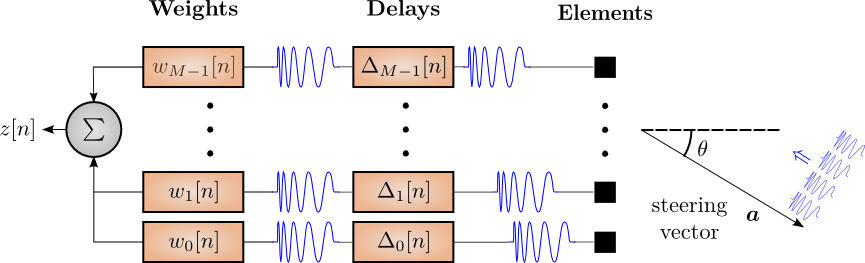
\includegraphics[width=3in]{gfx/beamforming_mv_lowres.png}
%\caption{}
%\label{II_fig:mv}
%\end{figure}

%Building and calculating the inverse of $\hat{R}$ is computational demanding, limiting the methods accessibility. Following the innovation in GPU computing, this has now started to change. 
%In this paper we introduce the first GPU implementation of the Capon beamformer capable of processing a 70 degree sector cardiac image from a 64 element phased array at interactive frame rates using both spatial and temporal smoothing. Both types of smoothing are important for maintaining delay-and-sum-like speckle and at the same time keep the high resolution property. This is achieved using complex base band data, which reduces the size of each range line to a minimum. In addition, complex data results in complex weights; hence this is a correct implementation of Capon beamforming with all degrees of freedom preserved. For high channel count systems we propose two ways of reducing computational complexity while maintaining 

\subsection{Beamspace Processing}\label{II_bs-capon}
Nilsen and Hafizovic \cite{Nilsen2009} have proposed to apply beamspace processing to reduce the required computations of the Capon beamformer when applied to medical ultrasound imaging. Beamspace is an alternative representation of the per-element data, transformed into a fan of beams covering the sector illuminated by transmit beams. The transformation is formally stated as
\begin{align}
\vec{x}_\text{BS}[n] &= \mat{B}\vec{x}[n], \ \ \ \ \ \ \ \ \ \ \ \ \ \, \mat{B} \in \mathbb{C}^{N,M} \label{II_eq:butler} \\ 
[\mat{B}]_{p,q} &= \frac{1}{\sqrt{M}}e^{-j 2 \pi p q / M} \ \ \ N \le M.
\end{align} 
The steering vectors in $\mat{B}$, the so-called Butler or normalized discrete fourier transform (DFT) matrix, determine each beam's direction in space. Beams where no interference is present can therefore be removed by simply removing rows from $\mat{B}$. 

For an imaging system using narrow transmit and receive beams, like cardiac ultrasound imaging, the received signal will be concentrated in a narrow band in wavenumber space. Hence, a small percentage of the beams will contain almost all the received energy. Nilsen and Hafizovic concluded that as little as three beams around (and including) the transmit direction were adequate to produce results comparable to applying Capon beamforming in element space. Hence, for equally pitched arrays the inversion steps is found to be constant with respect to the number of array elements.

The beamspace version of the Capon beamformer is derived by replacing the covariance matrix in (\ref{II_eq:w}) with the beamspace covariance matrix 
\begin{align}
\mat{\hat{R}}_\text{BS} = f(\vec{x}_\text{BS}) = f(\mat{B}\vec{x}), 
\end{align}
where $\mat{B} \in \mathbb{C}^{N_b,L}$, $N_b$ is the number of selected beams, and $f(\cdot)$ represent the covariance estimation process as defined in (\ref{II_eq:diag}).

In the remaining sections, the methods described in this section and Section \ref{II_sec:es-capon} will be referred to as beamspace Capon (BS-Capon) and element-space Capon (ES-Capon) respectively. The name Capon will refer to both methods. 

\subsection{GPU Compute Model}

%\textbf{(Ta med mer banale ting, dette er GPU for ultralydfolk)}

%\textbf{(Etter denne så må de forstå GPU og hvorfor MV passer.)}

In this section we give a brief discussion of GPU computing, laying the basis for our discussions on parallel implementation strategies. The Capon beamformers have been implemented using the CUDA GPU framework by Nvidia \cite{Nvidia2013}, however the challenges and proposed methods described in this paper are valid for other GPU framworks as well, like e.g. OpenCL. Independent of framework, the key point is that GPUs are designed to execute large sets of small concurrent tasks, like beamforming a pixel in a large image, much faster than a CPU. While the CPU has few cores, but logic to process complex threads, the GPU has many cores, but each core needs many (preferably simple) threads to keep it occupied and by that achieve maximum throughput.

In CUDA programming a kernel function is executed over a large set of threads, where the kernel function describes the work to be done in each thread. As depicted in Fig.\ \ref{II_fig:gpulayout}, threads are organized in a grid of thread-blocks, with maximal size of 1024 threads per block (e.g. $32\times32$). Threads inside a block support low-cost synchronization if needed. From a CUDA perspective the GPU consist of one or more streaming multi-processors (SM), where each SM is capable of executing multiple arithmetic operations per clock cycle.
%32 or more concurrent multiplications or additions, or both, depending on the architecture. A group of blocks is scheduled to each SM until all blocks have been processed.

An SM has a limited amount of shared memory (or near-core cache) and registers. Therefore, to achieve maximum GPU occupancy (defined as having the maximum number of threads residing on each SM), a conservative use of registers and shared memory per thread is required. Each thread should perform enough instructions per transferred byte in order to hide memory latency, and the problem should be divided into enough threads in order to hide instruction latency. Global GPU memory transactions, in addition to CPU-GPU transfers, are slow and must be minimized. All of these constraints combined pose a real challenge as the target problem has to map well to the GPU framework on both a grid, block, thread, and memory consumption level in order to benefit from parallel acceleration. In the next two sections, we will describe how this mapping can be done for the Capon beamformers.    

\begin{figure}
\centerline{\includegraphics[width=3.5in]{gfx/gpu_layout_vertical_2.eps}}
\caption{Calculation of Capon adaptive weights mapped to GPU architecture. A recorded echo across the array for a given range and angle (selected cell) is assigned to a group of $L$ threads that can run independently of all other groups. Note that several samples can be processed per thread-block if $L$ is small. The task of these $L$ threads is to calculate the Capon beamformer output in the three depicted steps.}
\label{II_fig:gpulayout}
\end{figure}

%When implementing algorithms on the GPU it is important to keep data as close to the core as possible. Utilizing available registers and shared memory to its maximum is therefore important.  

%More important, the CUDA 2.x compute capability (CC) has available 48 KB of near-core shared memory per SM that can be utilized by resident blocks. The maximum number of resident blocks per SM is 8, but in addition the maximum number of resident warps per SM is restricted to 48. Hence, with a block size of 512 only $48/(512/32) = 3$ blocks can occupy the SM at once. In addition, if one thread where to use 64B of shared memory the number of allowed resident blocks with a block size of 512 would be reduced to 1. Up to a curtain point it is beneficial to have as many warps as possible occupying the SM at once to hide latency from accessing memory. The SM has for CC 2.x 32K 32-bit long registers. When implementing algorithms on the GPU it is important to keep data as close to the core as possible. Utilizing available registers and shared memory to its maximum is therefore important.  

%\subsection{Optimizing kernel launch}
%Set the size of grid adaptively based on $L$, $M$ and $Yavg$.
%It is better to slide in space than time. $K$ is typically much larger than $2*Yavg + 1$.

% needed in second column of first page if using \IEEEpubid
%\IEEEpubidadjcol

\section{Parallel ES-Capon}\label{II_sec:meth}

In this section we will give a brief summary of our parallel implementation of the ES-Capon beamformer as presented in \cite{Asen2012} and \cite{Buskenes}. This implementation was our starting point when the BS-Capon beamformer was implemented.   

If the beamformer in (\ref{II_eq:z_mv}) is analyzed in combination with the matrix equation in (\ref{II_eq:b}) and the covariance estimation process in (\ref{II_eq:diag}), we see that the calculation of a set of Capon weights is independent across the outputs $z[n]$. As shown in Fig.\ \ref{II_fig:gpulayout}, a first level of granularity is therefore to divide the image into a grid, where the output in each cell can be calculated independently. Further, based on memory dependencies and to hold memory consumption per thread at a minimum, a group of threads should process one output in the final image. Continuing with the calculation of one weight vector, the algorithm can be broken down into three main steps that, to some extent, can be divided further into a set of parallel processes. That is, for each data vector $\vec{x}$ in the image:
\begin{align*}
%\begin{array}{l}
\text{1) } &\text{Calculate the sample covariance matrix } \mat{\hat{R}} \text{ as in } \text{(\ref{II_eq:diag})}.\\
\text{2) } &\text{Solve the linear system of equations as in (\ref{II_eq:b}}).\\ %\vec{b} =\mat{\hat{R}}^{-1}\vec{1}_L\\
\text{3) } &\text{Calculate } \vec{w} = \vec{b}/\vec{1}_{L}^H\vec{b} \text{ and the amplitude as in (\ref{II_eq:z_mv})}.
%\end{array}
\end{align*}
%\begin{enumerate}
%\item Calculate the sample covariance matrix $\mat{\hat{R}}$ as in (\ref{II_eq:R})
%\end{enumerate}
%\begin{enumerate}
%\item[2)] Solve the linear system of equations $\mat{\hat{R}}\vec{b} =\vec{ 1}$
%\end{enumerate}
%\begin{enumerate}
%\item[3)] Calculate $\vec{w} = \vec{b}/\vec{1}^H\vec{b}$ and the amplitude $\vec{w}^H\vec{x}$
%\end{enumerate}
The computational complexities of these three steps are $O(N_KN_LL^2)$, $O(L^3)$, and $O(L)$, respectively. As $M$ (and thereby $L$) increases, the first two steps quickly become unmanageable, and real-time performance in cardiac ultrasound imaging can only be achieved by exploring methods with reduced complexity.

%(The three steps have, for modularity, been implemented using three different kernels. Joining all kernels into one could possible lead to an increase in speed.)

%\begin{figure}
%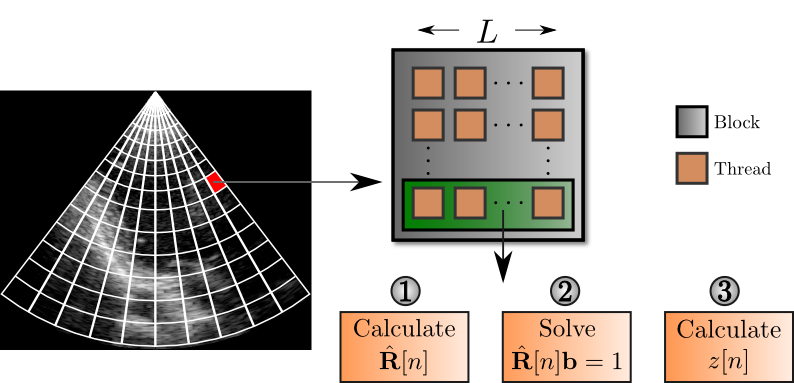
\includegraphics[width=3in]{gfx/gpu_layout_lowres.png}%
%\caption{}
%\label{II_fig:gpulayout}
%\end{figure}

\subsection{Calculation of Multiple Sample Covariance Matrices}\label{II_sec:calcR}

%The straightforward sum in (\ref{II_eq:R}) has complexity $O(L^2N_LN_K) = O(L^3)$ since $N_L$, the number of subarrays, is a function of $L$. This is actually the same as for inverting an $L \times L$ matrix. However little attention has been devoted to this step in the literature before. Note that for a typical array configuration we do more spacial smoothing than temporal smoothing. Hence, $N_K$ is usually small compared to $N_L$. The construction of $\mat{\hat{R}}$ is dominated by the number of elements $M$ ($N_L = M - L + 1$) for short subarrays, but since $L$ is selected in most cases to be between $M/2$ and $M/4$ a large $M$ implies a large $L$.

Calculation of one element of \R is from (\ref{II_eq:R}) found to be independent of calculation of the other elements. A natural level of granularity would then be to assign one thread to each element of $\mat{\hat{R}}$ \cite{Chen2011}. This will minimize global reads and writes needed per thread, but since we want to avoid block-to-block synchronization, the maximum supported subarray length is limited to 32 by this approach. Since most medical ultrasound arrays have 64 elements or more, an implementation not limited by $L_{max}=M/2=32$ is preferable.

In \cite{Asen2012, Buskenes} we demonstrated how the cubic complexity with $L$ %and linear complexity with $N_K$ 
can be reduced by realizing that calculations in (\ref{II_eq:R}) overlap across subarrays. %Element $(i,j)$ of $\mat{\breve{R}}[n]$ can be calculated from element $(i-1, j-1), \text{for } i,j \in [1, L-1]$ in a sliding window maner as
%\begin{align}
%\mat{\breve{R}}_{i,j}[n] &=  \mat{\breve{R}}_{i-1,j-1}[n]  \nonumber \\
%&+ \sum_{n'=n-K}^{n+K} (x_{i+N_L-1}[n']x_{j+N_L-1}[n']^* \nonumber \\
%&- x_{i-1}[n']x_{j-1}[n']^H). \label{II_eq:sliding}
%\end{align}
%Along the time dimension we also find that
%\begin{align}
%\mat{\breve{R}}[n] &= \mat{\breve{R}}[n-1] + \sum_{l=0}^{N_L-1} (\vec{x}_l[n+K]\vec{x}_l[n+K]^H \nonumber \\
%&- \vec{x}[n-K-1]\vec{x}[n-K-1]^H).
%\end{align}
%- \mat{\breve{R}}[n-K-1] + \mat{\breve{R}}[n-K].
%Sliding windows across subarrays and in time can be realized simultaneously if $\mat{\hat{R}}$, averaged over subarrays, is calculated from an $N_K$-average in time of the outer products $\vec{x}[n]\vec{x}[n]^H$. However, since $N_K$ typically is small, and the GPU has a limited amount of shared memory available per thread, we focus on subarrays only. 
%In that case, 
The complexity of calculating $\mat{\hat{R}}$ is by this reduced to $O(N_K(L(N_L-2)+2L^2))$. For $L=M/2$ this reduces to $O(N_KM^2)$.
%The sliding-window approach will cause dependence among the iterative calculations. The level of task granularity is therefore increased. Calculations are still independent across time, but not along diagonals of $\mat{\hat{R}}$. One thread is therefore assigned to each diagonal in the upper triangle of $\mat{\hat{R}}$. For small values of $L$, several covariance matrices are calculated per thread block (Fig. \ref{II_fig:gpulayout}). 
Maximum supported $L$ is also increased to the maximum number of threads per block (currently 1024). %However, for small-$L$-high-$M$ configurations, memory consumption per thread will be too high to achieve full GPU occupancy.

%Taking symmetry into account, only the upper half of $\mat{\hat{R}}$ needs to be calculated. However, the GPU computes $\mat{\hat{R}}$ in such a way that the lower triangle can be found with little overhead \cite{Buskenes}. This also means that no special solver is needed in order to solve $\mat{\hat{R}}\vec{b} = \vec{1}_L$, even if a symmetric solver could have saved some instructions.

%For the adaptive diagonal loading factor in (\ref{II_eq:diag}), the trace of $\mat{\hat{R}}$ has to be known before diagonal elements are written back to global memory. One row for all covariance matrices is written to global memory per kernel iteration, the diagonal elements therefore need to reside in shared memory until the trace is accumulated. When that is done, scattered writes of the scaled diagonal elements to global memory has to be performed.

%For subarray averaging, the first row and column of $\mat{\hat{R}}$ has to be fully calculated, and for time averaging $\mat{\hat{R}}[0]$ has to be fully calculated.

%Since $L$ usually is larger than $N$, we have 

%Building $\hat{\mat{R}}$ using a sliding window approach across $K$ and $N_{avg}$. We have a limited amount of fast, near-core memory on the GPU. On NVIDIA architecture this memory is known as shared memory, and is restricted to 48KB per compute block. The maximum block size of 32x32, further restrict how large arrays we can handle inside a single compute block. It is therefore natural to restrict $L$ to a maxima of $32$ elements. Since $L \le M/2$, $M \le 64$. We can not afford to hold the full $\hat{\mat{R}}$ ($M = L$) when $\hat{\mat{R}} > 32$, because of limited amount of memory. ... Explain in detail how \texttt{buildR} is implemented in a kernel. ... Give more details on how much shared memory we have, and how it can be divided between compute blocks occupying one stream multiprocessor (SM).

%Discuss the bottleneck adaptive diagonal loading causes. Possible solutions includes, use trace from previous image, use pre-calculated array power, constant weight.

%Time averaging takes a lot of resources. It has been shown that time averaging can maintain both resolution and delay-and-sum-like speckle. The same speckle statistics can be obtain with small subarrays, but then we loose resolution. Small sub-arrays benefits from being less computational demanding.   

%\subsubsection{CUDA Compute Model}
%The CUDA compute model is based on execution of a kernel across a grid of compute threads. Each position in the grid holds a block of threads. Each block is further divided into groups of 32 threads, known as a warp. The maximum number of threads inside a block is restricted to 512, hence 16 warps. From a CUDA perspective the GPU consist of one or more stream multi processors (SM), %where each SM is capable of 32 or more, depending on the architecture, concurrent multiplications and/or additions. The CUDA 2.x compute capability (CC) has available 48 KB of near-core shared memory per SM that can be utilized by resident blocks. The maximum number of resident blocks per SM is 8, but in addition the maximum number of resident warps per SM is restricted to 48. Hence, %with a block size of 512 only $48/(512/32) = 3$ blocks can occupy the SM at once. In addition, if one thread where to use 64B of shared memory the number of allowed resident blocks with a block size of 512 would be reduced to 1. Up to a curtain point 
%it is beneficial to have as many warps as possible occupying the SM at once to hide latency from accessing memory and executing time consuming mathematical functions. The SM has for CC 2.x 32K 32-bit long registers. When implementing algorithms on the GPU it is important to keep data as close to the core as possible. Utilizing available registers and shared memory to its maximum is %therefore important.   

\subsection{Solving Multiple Small Linear Systems}
%The literature has mostly focused on large systems when solving systems of linear equations on the GPU. GPU libraries therefore often lack a comprehensive collection of batched solvers for large sets of small systems. The reason for this is two-fold. First the GPU needs to solve thousands of small systems in order to beat the low memory latency of the CPU. Second there is a range of system dimensions that does not fit well with the GPU architecture, where only a small amount of shared memory and registers are available. Because of this, it has been proven hard to optimize a manageable set of solvers that provides speedups compared to the CPU in every case. 

In \cite{Asen2012} we discussed how it is not given that solving on the GPU is faster than solving on the CPU in general. However, there are two arguments for solving on the GPU. First the CPU, which might already run a lot of ultrasound-related algorithms, is offloaded. Second, the transfer of several thousand covariance matrices over the PCI-Express bus, from the CPU to the GPU, is avoided.

For the results presented in this paper, we have used a GPU implementation of batched Gauss-Jordan elimination made by Nvidia to solve $\mat{\hat{R}}\vec{b} = \vec{1}_L$, where $\vec{b} = \mat{\hat{R}}^{-1}\vec{1}_L$, for all pixels in an image in one kernel launch. The solver is available online for registered CUDA developers \cite{Nvidiaa}.%For smaller systems, $L < 10$, a direct solver using one thread per system is preferable. For this purpose we have implemented Cramer's rule for $2 \times 2$, $3 \times 3$ and $4 \times 4$ matrices. All solvers have been benchmarked against the latest Intel MKL libraries.

%However we will go through an implementation of an $\mat{U}^H\mat{D}\mat{U}$-decomposition-based solver to point out challenges when implementing batched solving of small linear systems on the GPU. ... (Unsure if this should be included).

%Can include details on GPU implementation of $\mat{U}^H\mat{D}\mat{U}$, but this has not proved to be faster than NVIDIA's GJ implementation. However, the complexity for solving with $\mat{U}^H\mat{D}\mat{U}$ decomposition is supposed to be $1/2$ of GJ.

%Skriv om utfordringene om å lage en solver på GPU. Ikke dra inn UHDU.

%In the final journal article we could discuss Conjugated gradient and Woodbury and the benefits they bring.
%Other solvers that provides different benefits includes Conjugated gradient and the use of the Woodbury matrix identity. 

\subsection{Compute Beamformer Output}
%The calculation of the beamformer output in (\ref{II_eq:z_mv}) has been implemented using one thread per element weight ($L$ threads per weight vector). After the solution vector $\vec{b}$ has been placed in shared memory, one of the $L$ threads finds the sum of $\vec{b}$. 
%Another option is to let several threads cooperate to form the sum using a binary reduction sum. However, in the following benchmarks the first approach has been used. 
%Each of the $L$ threads then reads one element of $\vec{b}$, and scales it with the inverse sum to get the weight vector $\vec{w}[n]$. 
The final output can be formed by either reducing the data down to length $L$ as in (\ref{II_eq:z_mv}), or increasing the weight vector to length $M$ as in (\ref{II_eq:z_mv2}). Since we selected to use $L$ threads per output, the data is reduced to length $L$ by letting thread $r$ calculate
%
\begin{align}\label{II_eq:subsum}
\breve{x}_{r} = \sum_{k=r}^{r+N_L-1}x_{k} \text{ for } r \in [0, L-1].
\end{align}
%
Each thread now computes $z_r = w_r^*x_r$, and finally one thread computes and outputs $z = \frac{1}{N_L}\sum_{r=0}^{L-1} z_r$ to global memory. %The last sum can also be performed using a binary reduction sum across several threads for increased speed.


\begin{figure}
\centerline{\includegraphics[width=3.2in]{gfx/gpu_layout_bs_2.eps}}
\caption{Calculation of the sliding beamspace transform. A group of $N_b$ threads is assigned a set of subarrays which they transform to beamspace in a sliding window fashion. In this example $N_b=3$, $l$ is the current subarray and $k$ is the current beam.}
\label{II_fig:gpulayoutbs}
\end{figure}

\section{Parallel BS-Capon}\label{II_sec:bs}

In this section we will derive a parallel implementation of the BS-Capon beamformer, and comment on how it deviates from the implementation in Section \ref{II_sec:meth}. The three main steps described in Section \ref{II_sec:meth} are present here as well, but in addition we need to transform the per-element data to beamspace. This can be done using a FFT, but for few beams ($N_b < \log{L}$) a matrix multiply with the truncated Butler matrix is less costly. 

In order to reduce the complexity of the matrix inversion problem the transformation must be performed before or after the covariance matrix has been estimated. If the transformation is applied before, one transformation is needed per subarray. This results in subarrays that no longer overlap. The amount of input data are therefore changed from $M$ to $N_LN_b$ elements per sample, but all remaining steps should get lower computational complexity as long as $N_b < L$.

The other option is to transform the element space covariance matrix to beamspace:
%
\begin{align}
\mat{\hat{R}}_\text{BS} &= \mat{B}\mat{\hat{R}}\mat{B}^H.
\end{align}
%
The advantage of this approach is that minor changes have to be made to the pipeline described in Section \ref{II_sec:meth}, but it will only speed up the solving step if the solution $\vec{b}_{BS}$ is transformed back to element space. In this paper we will focus on the first approach, and how it has been implemented on the GPU.
%By this approach we go from solving $\mat{\hat{R}}\vec{b} = \vec{1}_L$, which is an $L \times L$ system, to solving the $N_b \times N_b$ system $\mat{\hat{R}}_{BS}\vec{b}_{BS} = (\sqrt{L}\vec{e}_1)$. Now, one can either choose to transform the subarray sums, as in (\ref{II_eq:subsum}), to beamspace or transform the result, $\vec{b}_{BS}$, back to element space. 
In both cases solving has to be performed against a beamspace steering vector
\begin{align}
\vec{a}_\text{BS} &= \mat{B}\vec{1}_L = \sqrt{L}\vec{e}_1,
\end{align}
where $\vec{e}_i$ has the value one in the $i$th position and zeroes elsewhere. Note that the factor $\sqrt{L}$ was not included in \cite{Nilsen2009}.

As mentioned, transforming subarrays into beamspace yields subarrays that no longer overlap. This means that the spatial overlap previously exploited when calculating the sample covariance matrix in element space is no longer available. On the other hand, since $N_b$ should be small ($N_b < 32$), one thread assigned to each element in $\mat{\hat{R}}_\text{BS}$ is now an option. A kernel similar to the one described in \cite{Chen2011} has therefore been implemented. The computational complexity of this step is now $O(N_KN_LN_b^2)$, which for $L=M/2$ is less than the complexity of building $\mat{\hat{R}}$ in element space as long as $N_b < \sqrt{M}$.

%The implementation calculating covariance matrices therefore needs to be adjusted to handle non-overlapping subarrays. The complexity of constructing the covariance matrix is changed to $O(N_b^2L)$, so constructing the covariance matrices will be faster in beamspace as long as $N_b < \sqrt{L}$.
%Derivation of sliding beamspace transformation. 
%We will now show how to minimize the amount of operations required for the beamspace transformation by utilizing the overlap between subarrays previously exploited when estimating the covariance matrix in element space. 
The overlap between subarrays that were exploited when estimating the covariance matrix in element space, can now be utilized when calculating the beamspace transform. 
Given a $M$ long data vector divided into $N_L$ subarrays, the beamspace transformation of the $l$th subarray for the $k$th beam is from (\ref{II_eq:butler}) found to be:
\begin{align}\label{II_eq:bs_formula}
x_{\text{BS},l,k} &= \mat{B}_k\vec{x}_l \,\,\,\,\,\,\,\,\, k \in [0, N_b-1] \\
&= \frac{1}{\sqrt{L}}\sum_{p=i}^{l+L-1}x_p e^{-j2\pi k(p-l)/L},
\end{align}
where $\mat{B}_k$ is the $k$th row of $\mat{B}$. %Manipulating this expression we find that for $l \in [1, L-1]$
%\begin{align}\label{II_eq:sliding_bs}
%x_{\text{BS},l,k} &= \frac{1}{\sqrt{L}}((x_{\text{BS},l-1,k} - x_{l-1})e^{-j2\pi k/L} \nonumber \\ &+ x_{i+L-1}e^{-j2\pi k(L-1)/L}) \nonumber \\
%&= \frac{1}{\sqrt{L}}(x_{\text{BS},l-1,k} - x_{l-1} + x_{i+L-1})e^{-j2\pi k/L}.
%\end{align}

%We denote this the sliding-window beamspace transformation (SBS), and it is equal to a normalized sliding DFT \cite{Lyons2003}. For $l=0$ a full computation has to be performed using (\ref{II_eq:bs_formula}).
This formula has been implemented using a normalized sliding DFT (SDFT)\cite{Lyons2003}.
%Equation (\ref{II_eq:sliding_bs}) shows that 
The SDFT allows us to still save instructions by utilizing the overlap between subarrays, but with an increase in task level granularity. In this situation, it might be tempting to use one thread per beam (index $k$) that calculates this beam for all subarrays. However, since the number of selected beams usually is small ($N_b \ll M$) we will end up with a large memory-per-thread ratio ($M/N_b$). Using one thread per beam is therefore not feasible for small-$N_b$-large-$M$ configurations. One solution, as depicted in Fig.\ \ref{II_fig:gpulayoutbs}, is to combine SDFT with full computations. A number of sub thread groups of size $N_b$ is created that targets different sets of subarrays which they transform using the SDFT algorithm. In that way, the number of threads per sample is increased and thus the memory-per-thread ratio is decreased. 

After solving $\vec{b}_\text{BS} = \sqrt{L}\mat{\hat{R}}_\text{BS}^{-1}\vec{e}_1$, the beamspace weight vector is calculated as
%
\begin{align}
\vec{w}_\text{BS} = \frac{\vec{b}_\text{BS}}{\sqrt{L}\vec{e}_1\vec{b}_\text{BS}} \in \mathbb{C}^{N_b}
\end{align}  
%
using one thread per beam, and applied to the beamspace data summed across subarrays,
%
\begin{align}
z[n] = \vec{w}_\text{BS}^H\sum_{l=0}^{L-1}\vec{x}_{\text{BS},l}. 
\end{align}
%Several pixels are calculated per thread block for small values of $N_b$ in order to achieve high GPU occupancy. The beamspace data summed across subarrays are calculated as part of the SBS kernel.   
%
%How do we calculate the number of possible subarrays $N_L$ with overlap $L-s$ in a data vector of length $M$.
%\begin{align}
%N_L = floor(\frac{M}{s}) - floor(\frac{L-1}{s})
%\end{align}
%
As presented in (\ref{II_eq:diag}), adaptive diagonal loading is performed by loading the sample covariance matrix with the average energy per element, that is $\text{trace}\{\mat{\breve{R}}\}/L$. When data are transformed into beamspace, a high percentage of the total energy is mapped to a small subset of beams. Therefore, if a set of high energy beams is selected, the average energy per beam will be higher than the average energy per element ($\text{trace}\{\mat{\breve{R}}\}/L < \text{trace}\{\mat{\breve{R}}_{\text{BS}}\}/N_b$). This means that less diagonal loading (smaller $d$) has to be applied when the covariance is estimated among beams and not elements. 

To summarize, by transforming data to beamspace the complexity of all subsequent steps is potentially reduced. Calculation of the covariance matrix is now $O(N_KN_LN_b^2)$, the inversion step is $O(N_b^3)$, and calculation of weights and the beamformer output are both $O(N_b)$. The added complexity of SDFT is $O(N_bL)$. To maximize performance, large adjustments to the processing pipeline described in Section \ref{II_sec:meth} is required. 

%(Go in detail about the implementation using sliding DFT).

%(Go in detail about what kind of modifications we need to do to each of the three steps)

%Note that $\mat{B}\mat{B}^H = \mat{I}$ and $\mat{B}^H\mat{B} \ne \mat{I}$ when $N_b < L$.

%Another way of computing the beamspace transformation is to transform the steering vector $\vec{a}$ and covariance vector $\mat{\hat{R}}$ beforing solving the following system of linear equations: $(\mat{B}\mat{\hat{R}}\mat{B}^H)^{-1}(\mat{B}a) = b_{BS}$.

%\subsection{Iterative Capon}
%The idea behind iterative Capon is to perform Capon using small subarrays in several iterations until there is only two subarrays to sum. In this way we fix the size of L, hence the complexity of solving $\mat{R}\vec{b} = \vec{1}$. However, for each iteration we re-obtain L-1 degrees of freedom until all are retrieved after $K = M-L+1$ iterations. Since subarray averaging has been applied to decorrelated the signal, we might loose this effect when reestablishing all degrees of freedom. The number of iterations should therefore be restricted to $K/2$ to equal the normal choice of $L = M/2$ when it comes to degrees of freedom. 
 

\section{Benchmarks}\label{II_sec:bench}

%Describe the computer system (CPU, GPU...). Describe the data that are processed (field II, Channel data from GE Vingmed).
% stolpediagram, med de ulike metodenes kjøretid oppehverandre.

\begin{figure*}[!t]
\centerline{
\subfloat[]{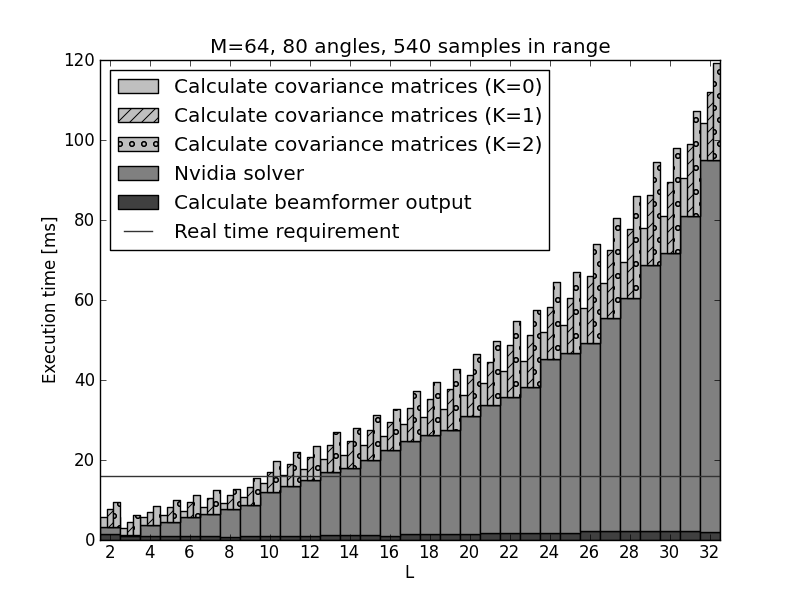
\includegraphics[width=3.4in]{gfx/benchmark_bar_64_80_540.png} \label{II_fig:benchUS64}}
\hfil
\subfloat[]{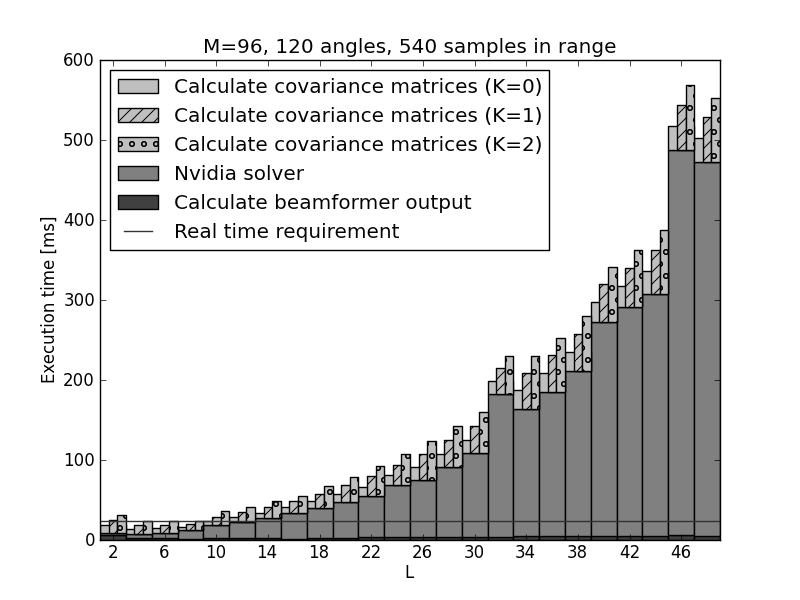
\includegraphics[width=3.4in]{gfx/benchmark_bar_96_120_540.png}%
\label{II_fig:benchUS96}}}
%\centerline{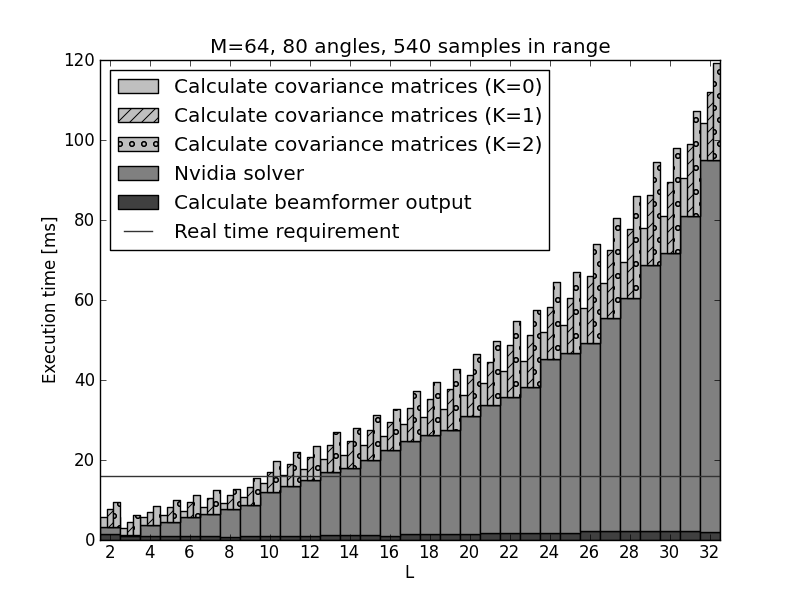
\includegraphics[width=3.5in]{gfx/benchmark_bar_64_80_540.png}}
\caption{Benchmarks of GPU Capon beamforming in element space for a cardiac image covering a $70\degree$ wide $15.4$ cm deep sector. Execution time is plotted as a function of subarray length $L$. The figures show execution times for the three steps listed in Section \ref{II_sec:meth}: Calculating covariance matrices with three different choices of temporal averaging, solver, and the final beamformer sum.}
\label{II_fig:bench}
\end{figure*}

\ifPhdDoc
  \begin{figure*}[!t]
  \centerline{\subfloat[]{\includegraphics[width=3.8in]{gfx/benchmark_bar_bs_M=64_Nx=80_Ny=540_Nb=3.png} \label{II_fig:benchBS64}}
%   \hfil
  \subfloat[]{\includegraphics[width=3.8in]{gfx/benchmark_bar_bs_M=96_Nx=120_Ny=540_Nb=3.png}%
  \label{II_fig:benchBS96}}}
\else
  \begin{figure*}[!t]
  \centerline{\subfloat[]{\includegraphics[width=3.4in]{gfx/benchmark_bar_bs_M=64_Nx=80_Ny=540_Nb=3.png} \label{II_fig:benchBS64}}
  \hfil
  \subfloat[]{\includegraphics[width=3.4in]{gfx/benchmark_bar_bs_M=96_Nx=120_Ny=540_Nb=3.png}%
  \label{II_fig:benchBS96}}}
\fi%
\caption{Benchmarks of GPU beamspace Capon beamforming for a cardiac image covering a $70 \degree$ and $15.4$ cm deep sector. Execution time is plotted as a function of subarray length $L$.  If $L$ had been fixed at $M/2$ and execution time was plotted against $N_b$, the solver would have shown the same quadratic growth as in Fig.\ \ref{II_fig:bench}. When $N_b$ is fixed, calculating the covariance matrix and the BS-transform is inverse proportional and proportional to $L$ respectively. The large jumps in execution times are caused by adaptive kernel launch configurations, which depends on $M$, $L$ and $N_b$.}
\label{II_fig:benchBS}
\end{figure*}
%
In this section we present benchmarks of the implementations presented in Sections \ref{II_sec:meth} and \ref{II_sec:bs} performed on a Nvidia Quadro 6000 graphics card (14 SMs, 1 TFlops theoretical single precision performance, 6 GB global memory, and 144 GB/s memory bandwidth). Problem sizes are calculated based on 64 and 96 element phased arrays with a 3.4 MHz center frequency. Assuming a system bandwidth of 80\% (relative to the center frequency) we need a complex sampling frequency of 2.7 MHz, and when imaging down to a depth of 15.4 cm we have approximately 540 samples per range line. The angular sampling is given by the Rayleigh criterion divided by two \cite{Hergum2007}, 
%
\begin{equation}\label{II_eq:rayleigh}
\delta{}\theta = \lambda/(2Mp),
\end{equation}
%
where $\lambda$ is the pulse wavelength and $p$ is the element pitch. 
To sample a $70\degree$ sector with $64$- and $96$-element arrays with $p=\lambda/2$ we therefore need approximately 80 and 120 receive beams respectively. 

The presented execution times do not include transfer of data from CPU- to the GPU-side, since data are assumed to be pre-delayed and available in global GPU memory. This is a valid assumption, since the imaging scenarios presented in this paper are well below the 8.0 GB/s limit of PCI Express 2.0. What is included are all calculations, memory transfers from global to shared GPU memory, and shared memory access. The delay step has previously been shown to take far less time than what we report for both Capon beamformers \cite{Song2012, Chen2011}.

Benchmarks of the ES-Capon beamformer are presented in Fig.\ \ref{II_fig:bench}. For each subarray size, the total execution time is split into one bar for each of the three steps described in Section \ref{II_sec:meth}, and the calculation of $\mat{\hat{R}}$ is presented for three different values of $K$. For $M=64$, $L=32$ and $K=2$, a typical setup for high-quality cardiac imaging, processing throughput is 8.3 frames per second (FPS). For $M=96$, $L=48$ and $K=2$ the processing throughput drops below $0.5$ FPS.

In Fig.\ \ref{II_fig:benchBS} we present similar benchmarks for the BS-Capon beamformer. The figure only presents results with use of temporal averaging ($K=2$). For $M=64$, $L=32$, $K=2$ and $N_b=3$, processing throughput is 125 FPS (8 ms). For $M=96$, $L=48$, $K=2$ and $N_b=3$, processing throughput is 77 FPS (13 ms). In all four benchmarks there is a line indicating the time it takes to acquire the underlying image using one receive line per transmit. Hence, below this line we are capable of performing real-time processing.

\section{In-vivo cardiac images}\label{II_sec:images}

%\begin{figure*}[!t]
%\centerline{
%\subfloat[]{ \includegraphics[width=2.2in]{gfx/das.png} \label{II_fig:phantomDAS} }
%\hfil
%\subfloat[]{ \includegraphics[width=2.2in]{gfx/capon.png} \label{II_fig:phantomMV} }
%\hfil
%\subfloat[]{ 
%\includegraphics[width=2.2in]{gfx/capon_bs.png} \label{II_fig:phantomBS} 
%\hfil
%\includegraphics[width=0.35in]{gfx/colorBarPhantom2.png}
%}
%}
%\caption{Simulated phantom containing one bright (20 dB) and one dark (-20 dB) circular area and two point targets (30 dB) in speckle (0 dB). The simulation was done using Field II with a 64-element, 3.4 MHz, and $\lambda/2$ pitch phased array. Dynamic range is -20 dB to 20 dB with mean value represented as 0 dB. The image is the 15th frame in the attached videos. a) Delay-and-sum with uniform weights. b) Element-space Capon ($L=32, K=2, d=0.1$) \multimedia{Media-Movie 1}. c) Beamspace Capon ($L=32, K=2, N_b=3, d=0.01$) \multimedia{Media-Movie 2}.}
%\label{II_fig:phantom}
%\end{figure*}

\begin{figure*}[!t]
\centerline{
\subfloat[]{\includegraphics[width=2.2in]{gfx/das_invivo.png} \label{II_fig:invivoDAS}}
\hfil
\subfloat[]{\includegraphics[width=2.2in]{gfx/capon_invivo.png} \label{II_fig:invivoMV}}
\hfil
\subfloat[]{
\includegraphics[width=2.2in]{gfx/capon_bs_invivo.png} \label{II_fig:invivoBS}}
\hfil
\includegraphics[width=0.4in]{gfx/colorBarInvivo2.png}
}
\caption{\textit{In-vivo} harmonic cardiac ultrasound image acquired using a 3.5 MHz, 64 elements phased array. Number of receive beams for the $70\degree$ sector is 98, and number of samples in range is 610. Dynamic range is -20 dB to 20 dB with mean value represented as 0 dB. The image is the first frame in the attached videos. a) Delay-and-sum with uniform weights \multimedia{Media-Movie 1}. b) Element-space Capon ($L=32, K=2, d=0.1$) \multimedia{Media-Movie 2}. c) Beamspace Capon ($L=32, K=2, N_b=3, d=0.01$) \multimedia{Media-Movie 3}.}
\label{II_fig:invivo}
\end{figure*}

%\begin{figure*}[!t]
%\centerline{
%\subfloat[]{\includegraphics[width=3in]{gfx/simulation_slice.png} \label{II_fig:simulationSlice}}
%\hfil
%\subfloat[]{\includegraphics[width=3in]{gfx/invivo_slice.png} \label{II_fig:invivoSlice}}
%}
%\caption{Lateral slices taken from the images in Fig. \ref{II_fig:phantom} and Fig. \ref{II_fig:invivo}. a) From Fig. \ref{II_fig:phantom} at 93 mm constant depth, through the two bright point scatterers. b) From Fig. \ref{II_fig:invivo} at 96 mm range, through the tip of the mitral valve.}
%\label{II_fig:slices}
%\end{figure*}

%To investigate the image quality of both the ES and BS-Capon beamformer, a phantom was simulated using Field II \cite{Jensen1992, Jensen1996a} (Fig. \ref{II_fig:phantom}). The simulation was performed using a 64-element, $p=\lambda/2$ pitch, 10 $\mu$m kerf, 80\% bandwidth, and 10 mm high phased array. The transducer was excited with a 3.4 MHz and $1.5\lambda$ long pulse with transmit focus at 90 mm. The phantom contains two circular areas, one bright at 20 dB and one dark at -20 dB, and two point targets at 30 dB, located at 90 mm depth. Speckle level is at 0 dB, covering an area from $\pm90\degree$ in azimuth. The resulting image has been processed both using DAS with uniform weights, ES- and BS-Capon. The presented image is frame $15$ in a series of images where motion is imposed on both circles, point targets and the probe. The entire simulation is presented in two attached videos \multimedia{Media-Movie 1 and 2}.

Fig.\ \ref{II_fig:invivo} presents results of applying ES- and BS-Capon on an \textit{in-vivo} image of the left ventricle. The image was acquired using a 64-element and $p=0.65\lambda$ pitched phased array in harmonic mode (1.7 MHz at transmit and 3.4 MHz at receive). The image frame is extracted from a cardiac cycle, that can be viewed in its full length in the attached videos \multimedia{Media-Movie 1, 2 and 3}.
The region of interest is 70\degree{} with a minimal lateral sampling of 98 receive beams given by (\ref{II_eq:rayleigh}).
The image was acquired using 50 transmit beams and "Synthetic Transmit Beamforming" was used on receive \cite{Hergum2007}.  %It is included to show that both ES-Capon and BS-Capon beamforming are feasible for \textit{in-vivo} cardiac imaging, not just in simulations.

%To get a better impression of the improved lateral resolution obtained with Capon beamforming, two slices taken from the images in Fig. \ref{II_fig:phantom} and \ref{II_fig:invivo} are included in Fig. \ref{II_fig:slices}. For the phantom, the cut goes through the two point targets at 90 mm constant radius, and for the cardiac image it goes through the tip of the mitral valve at 96 mm constant radius.

%Both data sets have 
The data set has been processed with the following settings for the ES-Capon beamformer: $L = 32$, $K = 2$, and $d=0.1$. These settings have previously been shown to provide improved lateral resolution while maintaining DAS-like speckle \cite{Synnevag2007a}. For BS-Capon the following parameters have been used: $L=32$, $K=2$, $d=0.01$, and $N_b=3$. 

%When the simulated phantom was processed with the ES-Capon beamformer, modulation effects were observed when the two bright point scatterers moved across receive-beams. The artifact did not disappear until 16x lateral oversampling relative to (\ref{II_eq:rayleigh}) was used on transmit. 
%The cardiac recording shows a 70\degree{} sector with a minimal lateral sampling of 98 receive beams given by (\ref{II_eq:rayleigh}). %Despite this, the same artifacts were not observed here. 
%The image was acquired using 50 transmit beams and "Synthetic Transmit Beamforming" was used on receive \cite{Hergum2007}. 

\section{Trading resolution for speed}\label{II_sec:trade}
As seen from Fig.\ \ref{II_fig:bench} the execution time, for the solver in particular, is reduced when $L$ is reduced. The same is true when $N_b$ is reduced in beamspace. So to gain an  increase in processing throughput we can reduce $L$ in element space or $N_b$ in beamspace. In this section we investigate how adjusting $L$ for ES-Capon and $N_b$ for BS-Capon impacts the lateral resolution. 

In Fig.\ \ref{II_fig:speed_res_trade}, the minimum distance between two point targets (while preserving a 6 dB saddle point in between the two) is plotted against $L$ (when processed with ES-Capon) and $N_b$ (when processed with BS-Capon). To produce the result in Fig.\ \ref{II_fig:speed_res_trade} $K=2$ and $d=0.01$ has been used on both methods in order to obtain the same resolution for $L=N_b=M/2$. 
In Fig.\ \ref{II_fig:invivo}, the diagonal loading factor for BS-Capon was adjusted to make the two results equal for $L=32$ and $N_b=3$. %The resolution for ES-Capon is therefore better here than what is presented in Fig. \ref{II_fig:phantom}. 
%We considered this to be a small value for ES-Capon and a normal value for BS-Capon (cf. Section \ref{II_sec:bs}), hence the resolution for ES-Capon is here better than what is presented in Fig. \ref{II_fig:phantom}.

The phantom used contained two point targets with 30 dB amplitude located at 90 mm depth. The two point targets were placed inside speckle, with 0 dB in amplitude, covering an area from $\pm90\degree$ in azimuth. The phantom was simulated using Field II \cite{Jensen1992, Jensen1996a}. The simulation was performed using a 64-element, $p=\lambda/2$ pitch, 10 $\mu$m kerf, 80\% bandwidth, and 10 mm high phased array. The transducer was excited with a 3.4 MHz and $1.5\lambda$ long pulse with transmit focus at 90 mm. The precision of the presented measurements is 0.12 mm, dictated by the simulated frame rate of 25 FPS, and the relative speed of the two point scatterers, 3 mm/s. To avoid having to deal with signal cancellation and errors caused by not hitting each point with a receive beam, 16x oversampling has been used on transmit. 

For high values of $L$ and $N_b$ the two methods are equal, but for lower values, BS-Capon provides improved resolution compared to using small subarrays. We see that the resolution for BS-Capon gradually decreases due to an automatic increase in diagonal loading (cf. end of Section \ref{II_sec:bs}). If we compensate by reducing $d$, BS-Capon will provide resolution equal to ES-Capon (with $L=M/2$) for all values of $N_b$ except one \cite{Nilsen2009}. For $N_b=1$ the resolution is worse than for DAS because of a triangular apodization caused by subarray averaging. 

In element space, resolution decays rapidly since the effective adaptive aperture is proportional to $L$. For $L = N_b=3$, BS-Capon provides almost 1 mm improved resolution over DAS and ES-Capon. However, note that the resolution of the Capon beamformers strongly depends on the image signal-to-noise ratio (SNR) and the choice of parameters. Thus, different SNR scenarios and choices of parameters will lead to different results. It is also worth noting that ES-Capon beamforming in this example performs worse than DAS for small values of $L$. For these small subarrays, the method is not able to steer zeros at each point target or accurately micro-steer the main lobe. Subarray averaging further impose a triangular or trapezoid apodization function, which leads to worse resolution if the introduced adaptivity can not compensate for the increase in main lobe width. For $L=1$ the ES-Capon is equal to DAS.

\begin{figure}
\centering
\includegraphics[width=3.3in]{gfx/speed_res_trade.png}
\caption{Trade-off between resolution and speed by reducing subarray size or reducing beamspace dimension. As $L$ or $N_b$ gets smaller, the execution time is reduced (Fig.\ \ref{II_fig:bench} and \ref{II_fig:benchBS}). When $N_b$ is varied, $L$ is fixed on 32.}
\label{II_fig:speed_res_trade}
\end{figure}

\section{Discussion}\label{II_sec:dis}
In this paper we have presented a parallel implementation of the BS-Capon beamformer for high-resolution cardiac ultrasound imaging. The results show that it is now possible to apply BS-Capon in real-time in cardiac ultrasound imaging by utilizing the power of a GPU. According to Fig.\ \ref{II_fig:benchBS} it is also possible to process two parallel receive lines per transmit beam (for both $M=64$ and $M=96$. $L=M/2$). %However, since we had to use oversampling in our simulation, these extra lines might be needed for increased sampling instead of increasing the frame rate. If parallel receive lines are used to obtain denser sampling, the acquisition time remains the same but the processing time is increased with a factor equal to the amount of oversampling. If parallel receive lines are used to increase the frame rate, the acquisition time is lowered, and the processing time remains constant. Hence, four parallel receive lines are not possible to process in real-time using BS-Capon with $N_b=3$ in combination with our single GPU setup.

For ES-Capon, processing rates for high quality settings are still too high to support real-time cardiac ultrasound imaging. From Fig.\ \ref{II_fig:benchUS64} we see that for $L = M/2 = 32$ and $K=1$, the total execution time is 110 ms (9 FPS). Taking into account that we use complex data, but less samples per image, these results are similar to the performance reported by Chen et al. \cite{Chen2011}.

A major part of the total execution time for ES-Capon comes from solving the system of linear equations. This limitation is targeted by reducing the sample covariance matrix size in beamspace, and as shown in Fig.\ \ref{II_fig:benchBS}, inverting the $3\times3$ beamspace covariance matrix is then barely visible. The time it takes to construct all covariance matrices is also reduced, but for few beams this is now the major contributor to the total execution time. If real-time is defined as 10 FPS \cite{Chen2011} almost all execution times in both Fig.\ \ref{II_fig:benchUS64} and \ref{II_fig:benchBS} are real-time. More natural for cardiac ultrasound imaging is to define real-time as the time it takes to acquire the underlying image. With this requirement the images formed using a 64 and 96 element array have a real-time requirement of 62.5 and 41.7 FPS respectively using single line acquisition. Each benchmark plot has a line indicating this real-time requirement. With beamspace processing, all processing times for large subarrays are below this line.

This paper further shows how to obtain a parallel formulation of the BS-Capon beamformer, and how to implement it in a GPU framework. The per-pixel granularity suggests that the beamformer is easily dividable across multiple GPUs. It is therefore possible to achieve higher frame rates if several GPUs are used simultaneously. However, there is usually a space-cost-energy limitation for how many GPUs that can be assembled in an ultrasound scanner.
 
%Turning to image quality we see from Fig. \ref{II_fig:phantom}, and the attached video of the simulation, that Capon beamforming provides improved lateral resolution of moving point targets both in element- and in a reduced beam-space ($N_b=3$). Our preliminary finding is that the Capon beamformers are local shift invariant as long as the lateral sampling is increased to a certain level in simulations \multimedia{Media-Movie 1 and 2}. %How large this oversampling factor needs to be and how the oversampling in the end is conducted will impact the real time requirement, and . 
%Future work should focus on how large this oversampling needs to be and how it should be conducted in order to still achieve real time processing.
%No major improvement in contrast is visually observed in the presented images and videos, other than slightly rounder circles due to mainlobe micro steering. 

Turning to image quality we see from Fig.\ \ref{II_fig:speed_res_trade} and the attached videos, that Capon beamforming provides improved lateral resolution of moving point targets both in element- and in a reduced beam-space ($N_b=3$). In the cardiac recording (Fig.\ \ref{II_fig:invivo}), structures are thinner and better resolved when the Capon beamformers are applied. One example is the mitral valve located at 10 cm depth and -1.5 cm width. On the other hand we observe a loss in contrast, especially in the septum (Fig.\ \ref{II_fig:invivo}, 6 cm depth, -2 cm width). This loss can be partially explained by the presence of highly correlated signals and mismatch between the assumed steering vector and signal. This is the same issue that made us use 16x oversampling when producing Fig.\ \ref{II_fig:speed_res_trade}. Future work should focus on how large this oversampling needs to be and how it should be conducted in order to still achieve real time processing.

In the end we want to point out that cardiac ultrasound has not been selected as the target modality in this paper because Capon beamforming shows large improvements in image quality in particular. It has been selected because it is the most computationally demanding modality, measured in floating points operations per second. The rationale being that if BS-Capon can run in real time for cardiac ultrasound it can run in real time for all medical ultrasound modalities. We believe that Capon beamforming may show more improvements in other imaging modalities where detection of small point targets is important.

%Nilsen and Hafizovic suggested to do automatic selection of beams in beamspace, hence picking the beams containing most energy. In this paper the center beams are always picked. This seems to work fine for focused systems, but an adaptive selection of beams should be implemented if interference at high angles is shown to contaminate the image.

%We expect that a large speedup had the Capon beamformer been implemented on the CPU using threads and SIMD (single instruction multiple data) instructions. 

%For a typical cardiac ultrasound image of 80*400 pixels (70 degree sector, 15cm range) acquired using a 2.5MHz, $M=64$ element phased array, the result is 10fps (subarray length $L=M/2$, temporal smoothing over 3 samples). If we do a 2-element pre-beamforming to get the channel count down to 32, the rate increases to 44fps. For a 32 element phased array we need less beams to cover the sector ($40 \times 400$ pixels), hence with the same parameters the frame rate increases to 87fps. The bottleneck of the Capon algorithm is to find the inverse covariance matrix for all pixels. This is an $O(L^3)$ operation, and results show that when L is larger than 16, real time performance is not possible for cardiac imaging with current high-end hardware. The target GPU has been Nvidia’s Quadro 6000, capable of 1Tflops.

\section{Conclusion}\label{II_sec:con}
In this paper a parallel formulation and implementation of the beamspace Capon beamformer have been presented, and
the beamformer has successfully been implemented on the GPU. For a three dimensional beamspace, processing rates supporting real-time cardiac ultrasound imaging was shown to be possible, meaning that processing rates higher than the image acquisition rate are obtained for a wide range of parameters. Image quality was investigated in an \textit{in-vivo} cardiac dataset. These results showed that Capon beamforming is feasible for cardiac ultrasound imaging, providing images with improved lateral resolution both in element- and beamspace.

%\section{Future work}
%Study shift invariance and minimum sampling...

%MLA's has, to some extent been used to increase later sampling. When using a high resolution beamformer, Nyquist tells us that the sampling frequency must be increase. Future work will concentrate on how much over sampling is required when using the Capon beamformer whit i curtain set of parameters...

%Plane waves...

% An example of a floating figure using the graphicx package.
% Note that \label must occur AFTER (or within) \caption.
% For figures, \caption should occur after the \includegraphics.
% Note that IEEEtran v1.7 and later has special internal code that
% is designed to preserve the operation of \label within \caption
% even when the captionsoff option is in effect. However, because
% of issues like this, it may be the safest practice to put all your
% \label just after \caption rather than within \caption{}.
%
% Reminder: the "draftcls" or "draftclsnofoot", not "draft", class
% option should be used if it is desired that the figures are to be
% displayed while in draft mode.
%
%\begin{figure}[!t]
%\centering
%\includegraphics[width=2.5in]{myfigure}
% where an .eps filename suffix will be assumed under latex, 
% and a .pdf suffix will be assumed for pdflatex; or what has been declared
% via \DeclareGraphicsExtensions.
%\caption{Simulation Results}
%\label{II_fig_sim}
%\end{figure}

% Note that IEEE typically puts floats only at the top, even when this
% results in a large percentage of a column being occupied by floats.


% An example of a double column floating figure using two subfigures.
% (The subfig.sty package must be loaded for this to work.)
% The subfigure \label commands are set within each subfloat command, the
% \label for the overall figure must come after \caption.
% \hfil must be used as a separator to get equal spacing.
% The subfigure.sty package works much the same way, except \subfigure is
% used instead of \subfloat.
%
%\begin{figure*}[!t]
%\centerline{\subfloat[Case I]\includegraphics[width=2.5in]{subfigcase1}%
%\label{II_fig_first_case}}
%\hfil
%\subfloat[Case II]{\includegraphics[width=2.5in]{subfigcase2}%
%\label{II_fig_second_case}}}
%\caption{Simulation results}
%\label{II_fig_sim}
%\end{figure*}
%
% Note that often IEEE papers with subfigures do not employ subfigure
% captions (using the optional argument to \subfloat), but instead will
% reference/describe all of them (a), (b), etc., within the main caption.


% An example of a floating table. Note that, for IEEE style tables, the 
% \caption command should come BEFORE the table. Table text will default to
% \footnotesize as IEEE normally uses this smaller font for tables.
% The \label must come after \caption as always.
%
%\begin{table}[!t]
%% increase table row spacing, adjust to taste
%\renewcommand{\arraystretch}{1.3}
% if using array.sty, it might be a good idea to tweak the value of
% \extrarowheight as needed to properly center the text within the cells
%\caption{An Example of a Table}
%\label{II_table_example}
%\centering
%% Some packages, such as MDW tools, offer better commands for making tables
%% than the plain LaTeX2e tabular which is used here.
%\begin{tabular}{|c||c|}
%\hline
%One & Two\\
%\hline
%Three & Four\\
%\hline
%\end{tabular}
%\end{table}


% Note that IEEE does not put floats in the very first column - or typically
% anywhere on the first page for that matter. Also, in-text middle ("here")
% positioning is not used. Most IEEE journals use top floats exclusively.
% Note that, LaTeX2e, unlike IEEE journals, places footnotes above bottom
% floats. This can be corrected via the \fnbelowfloat command of the
% stfloats package.



%\section{Conclusion}
%The conclusion goes here.





% if have a single appendix:
%\appendix[Proof of the Zonklar Equations]
% or
%\appendix  % for no appendix heading
% do not use \section anymore after \appendix, only \section*
% is possibly needed

% use appendices with more than one appendix
% then use \section to start each appendix
% you must declare a \section before using any
% \subsection or using \label (\appendices by itself
% starts a section numbered zero.)
%


%\appendices
%\section{Proof of the First Zonklar Equation}
%Appendix one text goes here.

% you can choose not to have a title for an appendix
% if you want by leaving the argument blank
%\section{}
%Appendix two text goes here.


% use section* for acknowledgement
\section*{Acknowledgment}
The authors would like to thank Prof. K. Kristoffersen, GE Vingmed Ultrasound and Norwegian University of Science and Technology, for valuable comments. 


% Can use something like this to put references on a page
% by themselves when using endfloat and the captionsoff option.
\ifCLASSOPTIONcaptionsoff
  \newpage
\fi



% trigger a \newpage just before the given reference
% number - used to balance the columns on the last page
% adjust value as needed - may need to be readjusted if
% the document is modified later
%\IEEEtriggeratref{II_8}
% The "triggered" command can be changed if desired:
%\IEEEtriggercmd{\enlargethispage{-5in}}

% references section

\ifPhdDoc
   \printbibliography[title=References,heading=subbibliography]
%    \bibliographysty
%    \bibliography{library.bib}
%    \print
\else


  % can use a bibliography generated by BibTeX as a .bbl file
  % BibTeX documentation can be easily obtained at:
  % http://www.ctan.org/tex-archive/biblio/bibtex/contrib/doc/
  % The IEEEtran BibTeX style support page is at:
  % http://www.michaelshell.org/tex/ieeetran/bibtex/
  \bibliographystyle{IEEEtran}
  % argument is your BibTeX string definitions and bibliography database(s)
  %\bibliography{IEEEabrv,../bib/paper}
  \bibliography{mybib} % link to mendeley organized bibtex-file
  %\bibliography{IEEEabrv,mybib} 
  % <OR> manually copy in the resultant .bbl file
  % set second argument of \begin to the number of references
  % (used to reserve space for the reference number labels box)
  %\begin{thebibliography}{1}

  %\bibitem{IEEEhowto:kopka}
  %H.~Kopka and P.~W. Daly, \emph{A Guide to \LaTeX}, 3rd~ed.\hskip 1em plus
  %  0.5em minus 0.4em\relax Harlow, England: Addison-Wesley, 1999.

  %\end{thebibliography}

  % biography section
  % 
  % If you have an EPS/PDF photo (graphicx package needed) extra braces are
  % needed around the contents of the optional argument to biography to prevent
  % the LaTeX parser from getting confused when it sees the complicated
  % \includegraphics command within an optional argument. (You could create
  % your own custom macro containing the \includegraphics command to make things
  % simpler here.)
  %\begin{biography}[{\includegraphics[width=1in,height=1.25in,clip,keepaspectratio]{mshell}}]{Michael Shell}
  % or if you just want to reserve a space for a photo:

  % insert where needed to balance the two columns on the last page with
  % biographies
  %\newpage

  \begin{IEEEbiography}[{\includegraphics[width=1in,height=1.25in,clip,keepaspectratio]{photos/jon_petter2.eps}}]{Jon Petter \AA{}sen}
  (S12) was born in Porsgrunn, Norway in 1986. He received the B.Sc. and M.Sc. degree in computer science from the University of Oslo, Norway, in 2008 and 2010. He is currently pursuing his Ph.D. degree in medical ultrasound technology at the Norwegian University of Science and Technology (NTNU) Medical Imaging Lab (MI-Lab), Trondheim, Norway. 

  He has industry experience from GE Vingmed Ultrasound, Horten, Norway, were he completed three summer internships from 2008 to 2010. His research interests include image and signal processing, adaptive ultrasound processing techniques and acceleration of ultrasound algorithms using Graphics Processing Units (GPUs). 
  \end{IEEEbiography}

  \begin{IEEEbiography}[{\includegraphics[width=1in,height=1.25in,clip,keepaspectratio]{photos/jo_inge2.eps}}]{Jo Inge Buskenes}
  received the B.Sc. degree in electrical engineering from Gj\o{}vik College University, Norway, in 2007, and the M.Sc. degree in instrumentation for particle physics from the University of Oslo, Norway, in 2010. He is currently pursuing the Ph.D. degree in image reconstruction and technology at the University of Oslo.

  His industry experience includes the European Organization for Nuclear Research (CERN), Geneva, Switzerland (2007-2008), and the Norwegian Defence Research Establishment, Kjeller, Norway (2009). He has lectured in digital signal processing at the Gj\o{}vik College University (2009), and at the University of Oslo (2010-2012). His research interests include adaptive beamforming, digital image reconstruction, high performance computing, intelligent detector design and embedded Linux platforms.
  \end{IEEEbiography}

  \begin{IEEEbiography}[{\includegraphics[width=1in,height=1.25in,clip,keepaspectratio]{photos/carl-inge.eps}}]{Carl-Inge Colombo Nilsen}
  (S’06–M’10) received the M.Sc. and Ph.D. degrees in computer science from the University of Oslo, Norway, in 2005 and 2010. He is currently working at the University of Oslo as a postdoctoral research fellow. His research interests include signal and array processing for ultrasound imaging and other acoustic applications.
  \end{IEEEbiography}

  % insert where needed to balance the two columns on the last page with
  % biographies
  %\newpage

  \begin{IEEEbiography}[{\includegraphics[width=1in,height=1.25in,clip,keepaspectratio]{photos/andreas.eps}}]{Andreas Austeng}
  was born in Oslo, Norway, in 1970. He received the M.S. degree in physics in 1996 and the Ph.D. degree in computer science in 2001, both from the University of Oslo. Since 2001, he has been working at the Department of Informatics, University of Oslo, first as a postdoctoral research fellow and currently as an associate professor. His research interests include signal and array processing for acoustical imaging.
  \end{IEEEbiography}

  %\newpage

  \begin{IEEEbiography}[{\includegraphics[width=1in,height=1.25in,clip,keepaspectratio]{photos/sverre.eps}}]{Sverre Holm}
  (M’82-SM’02) was born in Oslo, Norway, in 1954. He received the M.S. and Ph.D. degrees in electrical engineering from the Norwegian Institute of Technology, Trondheim, in 1978 and 1982, respectively. His academic experience includes Yarmouk University in Jordan (1984-1986) and the Norwegian Institute of Technology and later the University of Oslo (1989-1994) as an adjunct professor. Since 1995, he has been a professor of signal processing in the Department of Informatics at the University of Oslo. In 2002, he was elected a member of the Norwegian Academy of Technological Sciences, and in 2009, he became an adjunct professor in the Norwegian University of Science and Technology (NTNU) Medical Imaging Lab, Trondheim. His industry experience includes GE Vingmed Ultrasound, Horten, Norway (1990-1994). He worked with Sonitor Technologies (2000-2005), where he developed ultrasonic technology that is the core of the indoor positioning system described in \textit{Scientific Americanin} 2008 as "a positioning system that goes where GPS can't." He has published about 130 publications internationally, plus about 10 patents. He has had sabbaticals at GE Global Research, NY (1998), and the Waves and 
  Acoustics Laboratory of ESPCI, Paris (2008-2009). He was an associate editor of the \textit{IEEE Transactions on Ultrasonics, Ferroelectrics, and Frequency Control} from 1997 to 2002. His research interests are medical ultrasound imaging, modeling of tissue-ultrasound interaction, and ultrasound positioning.
  \end{IEEEbiography}


  % You can push biographies down or up by placing
  % a \vfill before or after them. The appropriate
  % use of \vfill depends on what kind of text is
  % on the last page and whether or not the columns
  % are being equalized.

  %\vfill

  % Can be used to pull up biographies so that the bottom of the last one
  % is flush with the other column.
  %\enlargethispage{-5in}


\fi



% \restoregeometry
}
   
% \else
%    Hello \newpage
% 
%    \pagestyle{fancy}
% 
%    \cleardoublepage
%    \includepdf[pagecommand={\thispagestyle{fancy}}, pages=-]{build/2_mvdr.pdf}
% \fi


\end{document}

%&header
% !TeX root = III_lca
\input{build/subheader.tex}
\endofdump





\newcommand\IEEEmembership[1]{}
% 
% \titleformat{\chapter}%command
% [display]%shape
% % {}%format
% {\flushright}%format
% {}%label
% {0pt}%sep
% {\color{Black}\Huge\bfseries}%before
% []%after
% \titlespacing*{\chapter}{0pt}{*0}{*2}


\renewcommand\thesection{\arabic{section}}
\renewcommand\thesubsection{\arabic{section}.\arabic{subsection}}

\providecommand\title[1]{} 
\renewcommand\title[1]{}

% \newcommand\title[1]{}
\providecommand\maketitle{}
\renewcommand\maketitle{}

% \titleformat{\chapter}[runin]{}
% {\put(-10,0){\color{SeaGreen}\Large\emph\thesection}}%  {\footnotesize \enspace \emph{Sec.}  }
%   {0pt}{\color{Black}\Large\bfseries\filright\textsl}[\vspace{15pt}\newline]
% \titlespacing*{\chapter}{0pt}{*4}{*0}


%\newcommand\title[1]{\makeatletter\def\mytitle{#1}\makeatother}
%\newcommand\maketitle{\makeatletter\meaning\@maketitle\makeatother}

\providecommand\author[1]{}
\renewcommand\author[1]{{\vbadness=99999}}

\providecommand\markboth[2]{}
\renewcommand\markboth[2]{}

% \newcommand\author[1]{}
\providecommand\thanks[1]{}
\renewcommand\thanks[1]{}
% \renewcommand\markboth[2]{}

% \ifOPTbeamer
%\newenvironment{narrow}[2]{%
%	\begin{list}{}{%
%			\setlength{\topsep}{0pt}%
%			\setlength{\leftmargin}{#1}%
%			\setlength{\rightmargin}{#2}%
%			\setlength{\listparindent}{\parindent}%
%			\setlength{\itemindent}{\parindent}%
%			\setlength{\parsep}{\parskip}}%
%		\item[]}{\end{list}}

\renewenvironment{abstract}%
{\vspace{2\baselineskip}\list{}{\footnotesize
\setlength{\topsep}{\parskip}%
\setlength{\leftmargin}{0pt}%
\setlength{\rightmargin}{0pt}%
\setlength{\listparindent}{\parindent}%
\setlength{\itemindent}{1cm}%\parindent
\setlength{\parsep}{\parskip}	
}%\rightmargin\leftmargin
\item[\textbf{Abstract ---}]\relax}
{\endlist\newpage}

% Options for the abstract package
%\setlength\absleftindent{0mm}
%\setlength\absrightindent{0mm}


%\newenvironment{IEEEkeywords}{}{}
%\excludecomment{IEEEkeywords}
\NewEnviron{IEEEkeywords}{
}

\newcommand\IEEEcompsoctitleabstractindextext[1]{#1}

\newcommand\IEEEdisplaynotcompsoctitleabstractindextext{}
\newcommand\IEEEpeerreviewmaketitle{} %\par\vspace*{\fill}\clearpage
%\renewcommand\maketitle{}

\renewcommand\AA{Å}

\newcommand\IEEEPARstart[2]{#1#2}

\newif\ifPeerReview\PeerReviewtrue              % Whether to create the PeerReview version or
% Journal version
\newif\ifOnlineColor\OnlineColortrue            % Compile online color version?
\ifOnlineColor
\newcommand\figPostfix{_online}              % Colored images online
\else
\newcommand\figPostfix{_bw}                  % Black and white in journal
\fi

\newif\ifCLASSOPTIONcompsoc\CLASSOPTIONcompsocfalse

\newif\ifCLASSOPTIONcaptionsoff\CLASSOPTIONcaptionsofffalse

\newcommand\appendices{\textsc{Appendix}}

\newenvironment{IEEEbiography}{}{}
% 

% These commands are already included in thesis.tex
\ifRootBuild\else
  \newglossaryentry{ASIC}{name={ASIC},
                  description={Application Specific Integrated Circuit} } 
                  
\newglossaryentry{ATR}{name={ATR},
                  description={Automatic Target Recognition} } 

\newglossaryentry{CPU}{name={CPU},
						description={Central Processing Unit} } 

\newglossaryentry{GPGPU}{name={GPGPU},
						description={General Purpose Graphics Processing Unit} } 

\newglossaryentry{GPU}{name={GPU},
						description={Graphics Processing Unit} } 
					
\newglossaryentry{MVDR}{name={MVDR},
						description={Minimum Variance Distortionless Response} } 
  \makeglossaries
  
%  \addbibresource{../LCAforActiveSonarImaging/references.bib}
\fi

\newif\ifBuildBibliography\BuildBibliographyfalse
% \usepackage[caption=false,font=normalsize,labelfont=sf,textfont=sf]{subfig}
%\usepackage{subfig}

%\let\Fig\undefined
\typeout{====Start of macro parse====}
\typeout{====Start of macro file====}

\providecommand\Fig{}
\renewcommand\Fig[1]{Fig.~\ref{#1}}
\providecommand\eq{}
\renewcommand\eq[1]{(\ref{#1})}

\providecommand\Grey[1]{{\color{Grey}#1}}
\providecommand\Red[1]{{\color{Red}#1}}
\providecommand\Blue[1]{{\color{Blue}#1}}
\providecommand\DarkBlue[1]{{\color{DarkBlue}#1}}
\providecommand\LightBlue[1]{{\color{LightBlue}#1}}
\providecommand\Brown[1]{{\color{Brown}#1}}
\providecommand\Green[1]{{\color{Green}#1}}
\providecommand\SeaGreen[1]{{\color{SeaGreen}#1}}
\providecommand\Yellow[1]{{\color{yellow}#1}}
\providecommand\Orange[1]{{\color{orange}#1}}

\providecommand*\nn{}
\renewcommand*\nn{\nonumber\\}

\providecommand\nmat{}
\renewcommand\nmat[1]{\begin{matrix}#1\end{matrix}}
\providecommand\bmat{}
\renewcommand\bmat[1]{\begin{bmatrix}#1\end{bmatrix}}
\providecommand\case{}
\renewcommand\case[1]{\begin{cases}#1\end{cases}}
\providecommand\textbox{}
\renewcommand\textbox[2]{\footnotesize\text{\parbox{#1}{\centering\emph{#2}}}}

\providecommand\rand{}
\renewcommand\rand{\text{rand}}
\providecommand\randn{}
\renewcommand\randn{\text{randn}}
\providecommand\rect{}
\renewcommand\rect{\text{rect}}
\providecommand\sinc{}
\renewcommand\sinc{\text{sinc}}
\providecommand\tr{}
\renewcommand\tr{\text{tr}}
\providecommand\adj{}
\renewcommand\adj{\text{adj}}

% \renewcommand\max{\text{max}}
\providecommand\argmin{}
\renewcommand\argmin[1]{\text{arg}\;\underset{#1}{\text{min}}}

\providecommand\qqquad{}
\renewcommand\qqquad{\quad\qquad}
\providecommand\qqqquad{}
\renewcommand\qqqquad{\qquad\qquad}

% renewcommand\l[1]{\left#1}
% renewcommand\r[1]{\right#1}

% {\text{\parbox{1.5cm}{\centering volume hyper- sphere}}}

%Keyword colouring:
\providecommand\kw{}
\renewcommand\kw[1]{#1}
\providecommand\parm{}
\renewcommand\parm[1]{#1}%\color{Black}#1\color{Black}}

\providecommand\of{}
\renewcommand\of[1]{\scriptstyle(\parm{#1})\displaystyle}
\providecommand\df{}
\renewcommand\df[1]{\scriptstyle[\parm{#1}]\displaystyle}
\providecommand\var{}
\renewcommand\var[3]{#1_\text{#2}\of{#3}}

\providecommand\diag{}
\renewcommand\diag{\text{diag}}

% \raisebox{lift}[extend-above-baseline][extend-below-baseline]{text}
\providecommand\mt{}
\renewcommand\mt[1]{\text{\emph{#1}}} %mt = mathtext
\providecommand\mathnorm{}
\renewcommand\mathnorm{\textstyle}
\providecommand\mathbig{}
\renewcommand\mathbig[1]{\displaystyle#1\mathnorm}
\providecommand\mathsmall{}
\renewcommand\mathsmall[1]{\scriptstyle#1\mathnorm}
\providecommand\mathtiny{}
\renewcommand\mathtiny[1]{\scriptscriptstyle#1\mathnorm}
\providecommand\sfrac{}
\renewcommand\sfrac[2]{\scriptstyle\raisebox{0.25pt}[0pt][0pt]{$\frac{#1}{#2}$}\mathnorm}
\providecommand\nfrac{}
\renewcommand\nfrac[2]{\textstyle\frac{#1}{#2}\displaystyle}

\providecommand\sumu{}
\renewcommand\sumu[1]{\sum\limits^{#1}\;}
\providecommand\suml{}
\renewcommand\suml[1]{\sum\limits_{#1}\;}
\providecommand\sumb{}
\renewcommand\sumb[2]{\sum\limits_{#1}^{#2}\;}

\providecommand\produ{}
\renewcommand\produ[1]{\prod\limits^{#1}\;}
\providecommand\prodl{}
\renewcommand\prodl[1]{\prod\limits_{#1}\;}
\providecommand\prodb{}
\renewcommand\prodb[2]{\prod\limits_{#1}^{#2}\;}

\providecommand\defeq{}
\renewcommand\defeq{\overset{\underset{\mathrm{def}}{}}{=}}

%Math macros:
\providecommand*\T{}
\renewcommand*\T{^{\scriptscriptstyle T}}
\providecommand\H{}
\renewcommand\H{^{\scriptscriptstyle H}}

\providecommand\vec{}
\renewcommand\vec[1]{\boldsymbol{#1}}
\providecommand\mat{}
\renewcommand\mat[1]{\boldsymbol{#1}}

\providecommand\Om{}
\renewcommand\Om{O_\text{m}}
\providecommand\Oa{}
\renewcommand\Oa{O_\text{a}}
\providecommand\Nl{}
\renewcommand\Nl{N_\text{l}}
\providecommand\Nk{}
\renewcommand\Nk{N_\text{k}}
\providecommand\1{}
\renewcommand\1{\vec 1}
\providecommand\I{}
\renewcommand\I{\mat I}
\providecommand\a{}
\renewcommand*\a{\vec a}
\providecommand\f{}
\renewcommand*\f{\vec f}
\providecommand\i{}
\renewcommand*\i{\vec i}
\providecommand\k{}
\renewcommand*\k{\vec k}
\providecommand\n{}
\renewcommand*\n{\vec n}
\providecommand\p{}
\renewcommand*\p{\vec p}
\providecommand\s{}
\renewcommand*\s{\vec s}
\providecommand\w{}
\renewcommand*\w{\vec w}
\providecommand\x{}
\renewcommand*\x{\vec x}
\providecommand\y{}
\renewcommand*\y{\vec y}

\providecommand\A{}
\renewcommand*\A{\mat A}
%\renewcommand*\B{\mat B}
%\renewcommand*\C{\mat C}
\providecommand\E{}
\renewcommand*\E{\mat E}
\providecommand\P{}
\renewcommand*\P{\mat P}
\providecommand\eP{}
\renewcommand*\eP{\mat{\hat P}}
\providecommand\R{}
\renewcommand*\R{\mat R}
\providecommand\Ri{}
\renewcommand*\Ri{\R^{-1}}
\providecommand\eR{}
\renewcommand*\eR{\mat{\hat R}}
\providecommand\eRi{}
\renewcommand*\eRi{\hat{\mat R}\;\!^{-1}}
\providecommand\Navg{}
\renewcommand*\Navg{N_\text{avg}}
\providecommand\W{}
\renewcommand*\W{\mat W}
\providecommand\X{}
\renewcommand*\X{\mat X}
\providecommand\Xd{}
\renewcommand*\Xd{\X_{\!\Delta}}
\providecommand\Y{}
\renewcommand*\Y{\mat Y}

\providecommand\L{}
\renewcommand*\L{\mat \Lambda}
%\renewcommand*\U{\mat U}
% renewcommand*\t{\mathtiny{^T}}
% \renewcommand*\h{\mathtiny{^H}}
\providecommand\t{}
\renewcommand*\t{^T}
\providecommand\h{}
\renewcommand*\h{^H}

\providecommand\minus{}
\renewcommand\minus{\scalebox{0.75}[1.0]{$-$}}

\ifPeerReview
\graphicspath{./submission/submit1}
\fi

% \newcommand\multimedia[1]{\textbf{{\color{red}[#1]}}}
\newcommand\multimedia[2]{\href{#1}{#2}}

% \newcommand\mediaPath{gfx/media}
\newcommand\articlePath{http://folk.uio.no/joibu/articles/2015_JOE_LCA}

\newcommand\mediaI{\multimedia{\articlePath/media1.mp4}{Media Movie~1}}
\newcommand\mediaII{\multimedia{\articlePath/media2.mp4}{Media Movie~2}}


\typeout{====done====}


\typeout{====Start document parse====}

% \usepackage{parskip}


\graphicspath{{../LCAforActiveSonarImaging/submission/final/}}
%~~~~~~~~~~~~~~~~~~~~~~~~~~~~~~~~~~~~~~~~~~~~~~~~~~~~~~~~~~~~~~~~~~~~~~~~~~~~~~~~~~~~~~~~~~~~~~~~~
\begin{document}
% 
\cleardoublepage
% \pagestyle{empty}

\providecommand*\papertitle{}\renewcommand*\papertitle{Low-Complexity Adaptive Sonar Imaging}

\mbox{}\hfill
\begin{minipage}{0.8\linewidth}
   \setlength\parskip{\baselineskip}
   \renewcommand\baselinestretch{1.1}

   \chapter*{Paper III}\label{ch:paperIII}
   \addcontentsline{toc}{chapter}{Paper III: \papertitle}
   \stepcounter{chapter}

   {\Large\bf \papertitle}

   J.I. Buskenes, R.E. Hansen and A. Austeng

   IEEE Journal of Oceanic Engineering\\
   Volume 42, Issue 1, January 2017%\\
   % \vfill
\end{minipage}


\cleardoublepage
\pagestyle{normal}
\renewcommand{\theHsection}{LCA\arabic{section}}
\renewcommand{\theHsubfigure}{Lca.\arabic{figure}.\arabic{subfigure}}
% \thispagestyle{plain}
\fancyhead[LE]{\bf Paper III}
\fancyhead[RO]{\bf\flushright \papertitle}
% \fancyhead[RE]{}
% \fancyfoot{}
% \fancyfoot[RO]{\thepage}
% \fancyfoot[LE]{\thepage}

\pdfbookmark[section]{Abstract}{lca_abstract}%

\begin{center}
{\Large\bf \papertitle}

\vspace{\baselineskip}
J.I. Buskenes, R.E. Hansen and A. Austeng
\end{center}

\overfullrule=1mm
% \graphicspath{{../HowtoHowtoCapon/submission/final/}}
{
\begin{refsection}[../LCAforActiveSonarImaging/references.bib]
%    \vboxbadness=99999 % Mute underfull vboxes, these are already reviewed
   % !TeX root = III_lca
\title{Low Complexity Adaptive Sonar Imaging}

\author{Jo~Inge~Buskenes, %
        Roy~Edgar~Hansen, %
        Andreas~Austeng%
\IEEEcompsocitemizethanks{\IEEEcompsocthanksitem All authors are with the Department of Informatics, University of Oslo, Norway.}%
\IEEEcompsocitemizethanks{\IEEEcompsocthanksitem R.~E.~Hansen is also with the Norwegian Defense Research Establishment (FFI), Norway.}% <-this % stops a space

% \thanks{Manuscript received April 19, 2005; revised January 11, 2007.}
}

% The paper headers
\markboth{IEEE Journal of Oceanic Engineering}%
{Low Complexity Adaptive Beamformer for Active Sonar Imaging}

% Publishers ID mark:
%\IEEEpubid{0000--0000/00\$00.00~\copyright~2007 IEEE}

% use for special paper notices
%\IEEEspecialpapernotice{(Invited Paper)}

% for Computer Society papers, we must declare the abstract and index terms
% PRIOR to the title within the \IEEEcompsoctitleabstractindextext IEEEtran
% command as these need to go into the title area created by \maketitle.
\IEEEcompsoctitleabstractindextext{%
\begin{abstract}
% 
% 
We have studied the low complexity adaptive (LCA) beamformer in active sonar imaging. LCA can be viewed as either a simplification of the minimum variance distortionless response (MVDR) beamformer, or as an adaptive extension to the delay and sum (DAS) beamformer. While both LCA and MVDR attempt to minimize the power of noise and interference in the image, MVDR achieves this by computing optimal array weights from the spatial statistics of the wavefield, while LCA selects the best performing weights out of a predefined set.

To build confidence in the LCA method we show that a robust MVDR implementation typically creates weight sets with shapes spanning between a rectangular and Hamming window function. We let LCA select from a set of Kaiser windows with responses in this span, and add some steered variations of each. We limit the steering to roughly half the \minus{}3\,dB width of the window's amplitude response. Using experimental data from the Kongsberg Maritime HISAS1030 sonar we find that LCA and MVDR produce nearly identical images of large scenes, both being superior to DAS. On point targets LCA is able to double the resolution compared to DAS, or provide half that of MVDR. This performance is achieved with a total of 6 windows; the rectangular window and the Kaiser window with $\beta=5$, in an unsteered version, and versions that are left and right steered to the steering limit. Slightly smoother images are produced if the window count is increased to 15, but past this we observe minimal difference. Finally we show that LCA works just as well if Kaiser windows are substituted with trigonometric ones.

All our observations and experiences point to LCA being very easy to understand and manage. It simply works, and is surprisingly insensitive to the exact type of window function, steering amount, or number of windows. It can be efficiently implemented on parallel hardware, and handles any scene without the need for parameter adjustments.

% \end{itemize}

\end{abstract}

% Keywords (normally not used for peer reviews)
\ifPeerReview\else
\begin{IEEEkeywords}
Beamforming, adaptive beamforming, MVDR, LCA, sonar, active, complexity.
\end{IEEEkeywords}
\fi
}
% \fi

% make the title area
\maketitle

% This command fixes abstract positioning for compsoc articles:
\IEEEdisplaynotcompsoctitleabstractindextext


% Insert page break and insert second title (peer review mode)
\IEEEpeerreviewmaketitle

\section{Introduction}


\IEEEPARstart{T}{he} best sonars in existence is perhaps found in nature. Bats, for instance, use a high frequency sonar to detect, identify and track prey with amazing precision in caves amongst a myriad of other bats. No man made sonar can currenly match this feat, much due to the challenge of processing and adapting to such a complex environment fast enough. This is why human made sonars have little to no adaptivity on transmit. However, several methods have been investigated to adaptively process the received acustic data. Perhaps the best studied method for reconstructing a sonar image out of such data is the minimum variance distortion-less response (MVDR) beamformer~\cite{Capon1969}. It adapts the sonar array's spatial response to minimize the influence of noise and interference in the final image.

In many cases MVDR can improve the contrast and resolution of active sonar images compared to conventional static methods~\cite{Blomberg2013,Blomberg2012a,Lo2004}. However, while the computational complexity of conventional beamformers are linear with the number of channels, O($M$), MVDR is at O($M^3$). This is because MVDR relies on estimating and inverting a covariance matrix. The estimation step dominates the computation in sonar systems with less than 32 channels, but here the computational complexity can be reduced and the implementation accelerated significantly using graphics computing units (GPUs)~\cite{Buskenes2014}. For larger systems the inversion step dominates. This can be dealt with by approximating the full covariance matrix with a small one using space reduction techniques such as beamspace processing~\cite{Asen2013}, or the closely related principal component analysis (PCA)~\cite{Kim2014}. Another alternative is to assume spatial stationarity to form more easily invertible Toepliz matrices~\cite{Asl2012}. However, the mentioned methods are still relatively slow compared to DAS.

A much faster and simpler alternative to MVDR is the Low Complexity Adaptive (LCA) beamformer. Based on an idea by Vignon~\cite{Vignon2008}, it was first introduced by Synnev\aa{}g \emph{et al}. in clinical medical ultrasound imaging~\cite{Synnevag2011}, who demonstrated its ability to obtain very similar image quality to MVDR in systems with focused transmit beams. LCA applies a set of predefined and static windows, or apodization weights, and selects the one offering the best noise suppression. It relies on the same optimization criterion as MVDR, thus may be considered a version of MVDR with a discrete and static window solution space. Alternatively, it may be viewed as a multi-apodization technique. One such method is described by Stankwitz \emph{et al}. in radar imaging~\cite{Stankwitz1995}, where the best out of 2 or 3 windows is selected. However, LCA differs in that it typically selects from a larger pool of windows and allows phase-steered variations of them. Phase-shifting the windows has the effect of slighly adjusting the angle the array is steered towards. This gives LCA an adaptive freedom that lies somewhere in between that of traditional multi-apodization techniques and MVDR. How similarly LCA performs compared to MVDR depends on how well the predefined windows represent the constrained solution space of MVDR.


Synnev\aa{}g \emph{et al}. suggested using a window set comprised of rectangular, Kaiser (or Kaiser-Harris) and inverted Kaiser functions. In total he let LCA choose from 12 unique windows, 6 of which were phase-shifted versions of a fairly wide Kaiser window, and one were rectangular. Synnev\aa{}g's composition of windows was motivated by the desire to use wide windows with maximum sidelobe suppression near the receiver, and narrow windows at greater depths for maximum sensitivity and depth penetration. While he achieved good results, it was not made clear how many windows LCA needs, or how they ideally should be steered. Also, it is not apparent how LCA performs in sonar systems where the transmit beam is unfocused.

In this study we expand our previous work of applying LCA to active sonar imaging~\cite{Buskenes2011}. We use variations of the parametric Kaiser window, but also compare it to the trigonometric window function. We extend Synnev\aa{}g's work by steering all our windows and not just some, and demonstrate how LCA's performance is affected by the type and number of windows included. Our results are obtained using experimental data from the 32 element Kongsberg Maritime HISAS1030 sonar, which operates at 100\,kHz with an \minus{}3\,dB element opening angle of 23$^\circ$. Although this system was designed as a synthetic aperture sonar (SAS) where an image is synthesized from several pings of data, we will only create images out of single pings (sectorscan imaging) in this study.

Our results show that when MVDR is robustified to work in active sonar imaging, it computes weights with spatial amplitude responses that tend to be symmetric and steered within a fraction of their \minus{}3\,dB widths. When letting LCA choose from Kaiser windows with similar responses, we obtain images with improved noise suppression and resolution. The resolution gain is made predictable by limiting the maximum steering to a fraction of the \minus{}3\,dB width of each window's spatial amplitude response. Overall, LCA produces images that are similar to MVDR, but with a resolution in between that of DAS and MVDR. LCA is also inherently robust, easy to implement, and fairly easy to understand.

This article is outlined as follows: In Section \ref{III_sec:beamforming} we offer a gentle introduction to beamforming. Then we move on to adaptive beamforming and describe the MVDR and LCA methods in \ref{III_sec:mvdr} and \ref{III_sec:lca}, respectively. We use LCA with the Kaiser window which we describe in \ref{III_sec:lca_kaiser_windows}, explain how we steer it in \ref{III_sec:lca_steering}, and by how much in \ref{III_sec:lca_steering_bounds}. Finally we add some remarks on using the trigonometric window instead of Kaiser in \ref{III_sec:lca_trigonometric}, and of of sampling considerations in \ref{III_sec:lca_oversampling}. Results and discussion are provided in Section \ref{III_sec:results_discussion}, where we study MVDR's windows to find suitable LCA ones in \ref{III_sec:results_lca_window_function}, assess the range of window types and steering in \ref{III_sec:results_window_parameters}, determine the number of windows needed in \ref{III_sec:results_database_size}, and add a note on computational complexity in \ref{III_sec:results_complexity}. Finally, Section \ref{III_sec:conclusion} provides a conclusion.
 

\section{Receive Beamforming}\label{III_sec:beamforming}

A sonar image is formed by estimating source locations and amplitudes. For this purpose a spatial bandpass filter is applied to the backscattered wavefield data. The filter is called an array processor or receive beamformer. The basic principle is to apply delay and weights to the sensor channels before summing them up, chosen such that signals from the location of interest are summed coherently, while other sources sum incoherently.

Assume that the wavefield has been sampled by an $M$ element uniform linear array, and that the signal signature has been removed by a matched filter. Let $x_m[\theta,n]$ be the delayed data from the $m$th channel, where the $\theta$ and $n$ are the azimuth angle and range sample of the focus point, respectively. Each angle $\theta$ will be processed independently, so to simplify notation we will assume the dependence on $\theta$ to be implicit from now on. 

The output $z[n]$ of a beamformer is defined as the weighted sum of all the delayed data samples:
%
\begin{align}
z[n] = \w\H[n]\x[n] = \bmat{w_0[n]\\w_1[n]\\\vdots\\w_{M-1}[n]}^H \bmat{x_0[n]\\x_1[n]\\\vdots\\x_{M-1}[n]},\label{III_eq:beamformer_output}
\end{align}
%
where $w_m$ is the weight factor assigned to channel $m$. A weight set is commonly called a window, apodization or taper function. When the window is real its response is symmetric. Applying a real window that trails off towards the edges creates a response with lower sidelobe levels and wider mainlobe, which translates into improved noise suppression at the cost of reduced resolution, respectively~\cite{Harris1978}.

Conventional beamformers all have static and usually real weights. The reference method is the delay-and-sum (DAS) beamformer, also know as the backprojection algorithm. It delays each pixel into focus, then applies a suitable window, and finally sums the data. The virtue of DAS is its simplicity, robustness to parameter errors, linear processing of the image and the ease of which it can be implemented in parallel hardware.

Adaptive beamformers are dynamic and seek to adjust the array response to better fit the incoming wavefield. This may be achieved by allowing either the weights or delays to change, or both. Here the weights are usually complex, which allows asymmetric responses. One of the most extensively studied adaptive methods is the minimum variance distortion-less response (MVDR) beamformer.

\section{MVDR}\label{III_sec:mvdr}

MVDR seeks to minimize the power of noise and interference in the output of the beamformer, under the constraint of unity gain in some desired direction $\phi$~\cite{Capon1969}. With the assumption of zero mean data this takes the form of minimizing output variance: 
%
\begin{align}
\argmin{\w[n]}\, E\{\big|z[n]\big|^2\} &= \argmin{\w[n]}\, \w[n]\R[n]\w\H[n]\nn
\text{subject to } \w^H[n]\a_\phi &= 1.\label{III_eq:mvdr_definition}
\end{align}
%
Here $\a_\phi$ is a steering vector for an azimuthal steering angle $\phi$, $E\{\cdot\}$ is the expectation operator, and $\R[n] = E\{\x[n]\x\H[n]\}$ is the spatial covariance matrix for the full array. This is a convex optimization problem with the unique solution:
%
\begin{gather}
\vec w[n] = \frac{\Ri[n]\a_\phi}{\a_\phi\T\Ri[n]\a_\phi}.\label{III_eq:mvdr_weights}
\end{gather}
The problem lies in estimating and inverting the spatial covariance matrix. We have described the exact steps in~\cite{Buskenes2014}: To avoid signal cancellation we apply spatial averaging by computing a mean covariance matrix from a set of subarrays with length $L$~\cite{Kailath1985}, for true speckle statistics we perform temporal averaging over $N_k = 2K+1$ temporal samples~\cite{Synnevag2009a}, and to improve robustness to parameter errors we add {\large$\epsilon$} percent of the total output power to the matrix's diagonal~\cite{Cox1987,Maksym1979}. These steps are also needed to ensure that the covariance matrix is numerically well conditioned and hence invertible.

\ifPhdDoc
   \begin{figure}[tbp]\centering%
   \includegraphics[width=.8\linewidth]{gfx/fig1.eps}%
\else
   \begin{figure}[tbp]\centering%
   \ifPeerReview%
      \includegraphics[width=.5\linewidth]{gfx/buske1_online.eps}%
   \else%
      \includegraphics[width=\linewidth]{gfx/buske1_online.eps}%
\fi\fi%
\caption{Each Kaiser window is steered in the interval $\phi\in[0, \phi_{\mathrm{3\,dB}}(\beta)]$. The angle $\phi_{\mathrm{3\,dB}}(\beta)$ is the amount of steering needed for the steered amplitude response to have a \protect\minus{}3\,dB crossing that is exactly half that of the unsteered window. With each window steered this way we expect the resolution gain to remain predictable and independent of $\beta$, and we also effectively constrain the white noise gain of the beamformer.}\label{III_windows_steering}
\end{figure}

\ifPhdDoc
   \begin{figure}[tbp]\centering%
   \includegraphics[width=.7\linewidth]{gfx/fig2.png}%
\else
   \begin{figure}[tbp]\centering%
   \ifPeerReview%
      \includegraphics[width=.5\linewidth]{gfx/buske2_online.png}%
   \else%
      \includegraphics[width=\linewidth]{gfx/buske2_online.png}%
\fi\fi%
\caption{The submerged object used to test beamforming resolution is a 1\,m by 1\,m test cross attached to an anchor with a diameter of approximately 13\,cm. Source image curtesy of Bundeswehr Technical Center for Ships and Naval Weapons, Maritime Technology and Research (WTD 71).}\label{III_cross}
\end{figure}


\ifPhdDoc
   \begin{figure*}[t]\centering%
   \makebox[\linewidth][c]{\includegraphics[width=1.25\linewidth]{gfx/fig3_phd.pdf}}
   \caption{\emph{Determining LCA window type}: MVDR image with typical frequency responses for windows used in various pixel regions.\\[.5\baselineskip]
   \textbf{Left:} MVDR sectorscan image of the oiltanker Holmengraa, with 40x40 pixel groups for the shadow, highlight and speckle region of the image indicated with red boxes.\\[.5\baselineskip]
   \textbf{Right:} MVDR window amplitude and phase responses computed from the 40x40 pixel groups. The responses are overlayed each other and the amount of overlap is colored using a logarithmic scale. The size of the pixel groups were chosen ad-hoc for the histograms to be visually invariant to a shift in position within the same region. Since each pixel is pre-delayed into focus the unsteered responses all have their center at broadside. The dashed red lines at -13\,dB and -43\,dB marks the peak sidelobe levels of an unsteered rectangular and Hamming window, respectively. Note how the responses are more or less symmetric, with very little steering in the shadow, moderate steering in speckle and steering within roughly 3\,dB in highlight. The phase varies most in the highlight region where we see the highest contrast.}\label{III_mvdr_selected_windows}
\else
\setcounter{topnumber}{1}
\setcounter{dbltopnumber}{1}

   \begin{figure*}[t]\centering%
   \includegraphics[width=\linewidth]{gfx/buske3_online.pdf}%
   \caption{\emph{Determining LCA window type}: MVDR image with typical frequency responses for windows used in various pixel regions.\newline
   \emph{Left:}\hfill
   \parbox[t]{.95\linewidth}{MVDR sectorscan image of the oiltanker Holmengraa, with 40x40 pixel groups for the shadow, highlight and speckle region of the image indicated with red boxes.}\protect\\\hspace{\textwidth}
   \emph{Right:}\hfill
   \parbox[t]{.95\linewidth}{MVDR window amplitude and phase responses computed from the 40x40 pixel groups. The responses are overlayed each other and the amount of overlap is colored using a logarithmic scale. The size of the pixel groups were chosen ad-hoc for the histograms to be visually invariant to a shift in position within the same region. Since each pixel is pre-delayed into focus the unsteered responses all have their center at broadside. The dashed red lines at -13\,dB and -43\,dB marks the peak sidelobe levels of an unsteered rectangular and Hamming window, respectively. Note how the responses are more or less symmetric, with very little steering in the shadow, moderate steering in speckle and steering within roughly 3\,dB in highlight. The phase varies most in the highlight region where we see the highest contrast.} }\label{III_mvdr_selected_windows}
\fi%

\end{figure*}

\ifPhdDoc
   \begin{figure*}[tbp]\centering%
   \makebox[\linewidth][c]{\includegraphics[width=1.25\linewidth]{gfx/fig4.pdf}}
%    \includegraphics[width=\linewidth]{gfx/fig4.pdf}%
   \caption{\emph{Determining Kaiser parameter boundaries}: LCA images of the resolution test cross and anchor created with a large window database, but where the upper bounds for $\beta$ and $\phi$ are varied. The upper left image is equal to DAS with a rectangular window. For all images we measure the lateral distance $\Delta x$ between the two \protect\minus{}3\,dB points of the anchor (red object). These are specified relatively to the reference distance  $\Delta x_\text{ref}$ from the upper left DAS image.
   \\[.5\baselineskip]
   \textbf{Upper bound $\beta$:} Observe that LCA gets better at suppressing sidelobes in the image as we increase the upper bounds for $\beta$. \Fig{III_mvdr_selected_windows} suggests that MVDR prefers windows with sidelobe levels lower than that of Kaiser with $\beta=2$, but here we observe further improvement going to $\beta=5$.
   \\[.5\baselineskip]
   \textbf{Upper bound $\phi$:} As we increase the upper bound of the steering $\phi$, we also increase the lateral image resolution.
   }
\else
   \begin{figure*}[t]%
   \includegraphics[width=\textwidth]{gfx/buske4_online.pdf}%
   \caption{\emph{Determining Kaiser parameter boundaries}: LCA images of the resolution test cross and anchor created with a large window database, but where the upper bounds for $\beta$ and $\phi$ are varied. The upper left image is equal to DAS with a rectangular window. For all images we measure the lateral distance $\Delta x$ between the two \protect\minus{}3\,dB points of the anchor (red object). These are specified relatively to the reference distance  $\Delta x_\text{ref}$ from the upper left DAS image.
   \newline
   \emph{Upper bound $\beta$:}\hfill
   \parbox[t]{.89\linewidth}{Observe that LCA gets better at suppressing sidelobes in the image as we increase the upper bounds for $\beta$. \Fig{III_mvdr_selected_windows} suggests that MVDR prefers windows with sidelobe levels lower than that of Kaiser with $\beta=2$, but here we observe further improvement going to $\beta=5$.}\newline
   \emph{Upper bound $\phi$:}\hfill
   \parbox[t]{.89\linewidth}{As we increase the upper bound of the steering $\phi$, we also increase the lateral image resolution. }
   }
\fi%
\label{III_oversampling_mosaic_bounds}
\end{figure*}

\setcounter{dbltopnumber}{2}

\ifPhdDoc
   \begin{figure*}[t]\centering
   \subfloat[$\beta$-values of the Kaiser window chosen for each image pixel. Note how LCA prefers a narrow response ($\beta=0$) on the anchor, and on other strong sources with little lateral interference. On the sources where lateral interference is present it chooses the widest response with the best sidelobe suppression.]{\makebox[\linewidth][c]{\includegraphics[width=1.25\linewidth]{gfx/fig5a.pdf}}%%
   \label{III_oversampling_mosaic_bounds_beta}}
   \hfil
   \subfloat[$\phi$-values of the Kaiser window chosen for each image pixel. On strong sources LCA selects windows that are steered away from the source. This is what improves the FWHM measurement in \Fig{III_oversampling_mosaic_bounds}.]{\makebox[\linewidth][c]{\includegraphics[width=1.25\linewidth]{gfx/fig5b_phd.pdf}}%
   \label{III_oversampling_mosaic_bounds_phi}}
   \caption{Kaiser windows chosen for each pixel in the image of the resolution test cross. The underlying image is the one shown in \Fig{III_oversampling_mosaic_bounds}, with the same parameters. The location of the anchor, cut line and main scatter locations of the cross is marked in red.}
   \label{III_fig_sim}
   \end{figure*}
\else
   \begin{figure*}[t]\centering
   \subfloat[$\beta$-values of the Kaiser window chosen for each image pixel. Note how LCA prefers a narrow response ($\beta=0$) on the anchor, and on other strong sources with little lateral interference. On the sources where lateral interference is present it chooses the widest response with the best sidelobe suppression.]{\includegraphics[width=\textwidth]{gfx/buske5a_online.pdf}%%
   \label{III_oversampling_mosaic_bounds_beta}}
   \hfil
   \subfloat[$\phi$-values of the Kaiser window chosen for each image pixel. On strong sources LCA selects windows that are steered away from the source. This is what improves the FWHM measurement in \Fig{III_oversampling_mosaic_bounds}.]{\includegraphics[width=\textwidth]{gfx/buske5b_online.pdf}%
   \label{III_oversampling_mosaic_bounds_phi}}
   \caption{Kaiser windows chosen for each pixel in the image of the resolution test cross. The underlying image is the one shown in \Fig{III_oversampling_mosaic_bounds}, with the same parameters. The location of the anchor, cut line and main scatter locations of the cross is marked in red.}
   \label{III_fig_sim}
   \end{figure*}
\fi

\ifPhdDoc
   \begin{figure*}[tb]\centering%
   \makebox[\linewidth][c]{\includegraphics[width=1.25\linewidth]{gfx/fig6.pdf}}%
\else
   \begin{figure*}[t]%\centering%
   \includegraphics[width=\textwidth]{gfx/buske6_online.pdf}%
\fi
\caption{\emph{LCA images using different window database sizes}. The window boundaries are the same. The upper left image is identical to a rectangularly weighted DAS. Observe that finer sampling of the $\beta$-range improves sidelobe suppression but leaves resolution unchanged. Adding more steering-variations improves both sidelobe suppression and resolution. However, using more than  $N_\beta=2$ window types and $N_\phi=3$ steering angles makes minimal difference.}\label{III_oversampling_mosaic}
\end{figure*}

\ifPhdDoc
   \begin{figure*}[t]\centering
   \subfloat[\emph{Image quality of approximate point scatterers found in the resolution test cross scene}. Two lateral image cuts are shown in the leftmost figures, along with the response of a rectangularly weighted DAS. Note how the FWHM of LCA sits in between that of DAS and MVDR. Also note how LCA is insensitive to the window type; its performance is near identical whether it uses Kasier or trigonometric windows.]{\makebox[\linewidth][c]{\includegraphics[width=1.25\textwidth]{gfx/fig7a.pdf}}%
   \label{III_beamformer_comparison_cross}}
   \hfil
   \subfloat[\emph{Image quality of the full sector Holmengraa scene}. Compared to DAS the adaptive beamformers produce deeper shadows, sharper edges and a higher detail level. The adaptive methods produce nearly identical images.]{\makebox[\linewidth][c]{\includegraphics[width=1.25\textwidth]{gfx/fig7b_phd.pdf}}%%
   \label{III_beamformer_comparison_holmengraa}}
   \caption{Comparing image quality of DAS, MVDR and LCA with Kaiser or trigonometric windows.}\label{III_image_quality}
   \end{figure*}
\else
   \begin{figure*}[t]\centering
   \subfloat[\emph{Image quality of approximate point scatterers found in the resolution test cross scene}. Two lateral image cuts are shown in the leftmost figures, along with the response of a rectangularly weighted DAS. Note how the FWHM of LCA sits in between that of DAS and MVDR. Also note how LCA is insensitive to the window type; its performance is near identical whether it uses Kasier or trigonometric windows.]{\includegraphics[width=\textwidth]{gfx/buske7a_online.pdf}%
   \label{III_beamformer_comparison_cross}}
   \hfil
   \subfloat[\emph{Image quality of the full sector Holmengraa scene}. Compared to DAS the adaptive beamformers produce deeper shadows, sharper edges and a higher detail level. The adaptive methods produce nearly identical images.]{\includegraphics[width=\textwidth]{gfx/buske7b_online.pdf}%%
   \label{III_beamformer_comparison_holmengraa}}
   \caption{Comparing image quality of DAS, MVDR and LCA with Kaiser or trigonometric windows.}\label{III_image_quality}
   \end{figure*}
\fi



\section{LCA}\label{III_sec:lca}

A much less complex alternative to MVDR is the low complexity adaptive (LCA) beamformer. It iterates through a set of $P$ windows and selects the window $p$ that best fulfills the minimum variance criterion:
%
\begin{align}
\argmin{p}\, E\{\big|z_p[n]\big|^2\} = \argmin{p}\, E\big\{\big|\w_{p}\H\x[n]\big|^2\big\}\nn
\qquad\text{subject to}\qquad \w\H\a_\phi = 1.\label{III_eq:lca_definition}
\end{align}\label{III_lca_criterion}
%
Note how closely LCA is related to the MVDR definition in \eq{III_eq:mvdr_definition}. The optimization criterion and constraint is the same, but LCA has a finite and discrete solution space for the weights. As will be demonstrated in Section \ref{III_sec:results_lca_window_function}, LCA performs similarly to MVDR because a robustified MVDR implementation seems to be constrained to window functions similar to the ones we let LCA choose from.

In practice, we estimate the beamformer output power by computing a sample power average $s_z^2$:
%
\begin{align*}
E\big\{\big|z[n]\big|^2\big\} \approx s_z^2 = \frac{1}{N_k} \sumb{n'=n-K}{n+K} \big| z[n'] \big|^2
\end{align*}
%
which computes the sample power average over $N_k=2K+1$ temporal samples. This is the same temporal averaging method we use for MVDR. In our case the bandwidth of our matched filtered signal is a just few samples long, hence $K=1$ will be used for both MVDR and LCA throughout this work.

If the pixels are correlated laterally, we can include a weighted combination of these to improve the variance estimation:
%
\begin{align}
s_z^2 = \frac{1}{N_x N_k} \sumb{\nmat{\scriptstyle x'=\\[-2mm]\scriptstyle x-X}}{x+X} \sumb{\nmat{\scriptstyle n'=\\[-2mm]\scriptstyle n-K}}{n+K} \omega[x',n']\big| z[x',n'] \big|^2
\end{align}
%
where $N_x = 2X+1$ is the number of azimuth lines to average over, and $\omega[x',n']$ is a normalized 2 dimensional weight function. Since we oversample slightly laterally when we delay each pixel (see Section \ref{III_sec:lca_oversampling}), we thought the lateral correlation to be sufficient to benefit from this. However, we observed no visual improvement from applying this technique, and decided not to use it.
% 

\subsection{Window function: Kaiser}\label{III_sec:lca_kaiser_windows}

As will be demonstrated in upcoming sections, the LCA beamformer works very well with windows generated from the Kaiser-Bessel function. We will express it in vector form as:
%
\begin{align}
\f_\beta = \bmat{
f_0(\beta) \\
\vdots\\
f_{M-1}(\beta)
}\label{III_eq:kaiser_window_vector}
\end{align}
%
where
%
\begin{align}
f_m(\beta) = \frac{I_0\left(\pi\beta\sqrt{1-\left(\frac{2m}{M-1}-1\right)^2}\right)}{I_0(\pi\beta)}\label{III_eq:kaiser_window_element}
\end{align}
%
and $I_0$ is the zeroth order modified Bessel function of the first kind:
%
\begin{align}
I_0(x) = \sumb{a=0}{\infty} \left[ \frac{\left(\frac{x}{2}\right)^a}{a!} \right]^2.\label{III_eq:modified_bessel_first_kind}
\end{align}
%
The Kaiser-Bessel window is near optimal in the sense of having its peak energy concentration around $\theta=0^\circ$, for a given space-bandwidth product related to the Kaiser parameter $\beta$ as:
%
\begin{align}
\beta = \frac{TB}{2},
\end{align}
%
where $T$ in our case is the spatial extent of the window and $B$ is its bandwidth. Adjusting $\beta$ changes the trade-off between mainlobe width and sidelobe level. When $\beta=0$ the window becomes rectangular, while at large values ($\beta>5$) the window converges to a Gaussian both in time and frequency. This class of windows is generally considered well suited for separating closely spaced sources with amplitudes of a high dynamic range~\cite{Harris1978}, they are easy to make, and they are optimal for any value of $\beta$.


\subsection{Steering}\label{III_sec:lca_steering}

Adding slightly steered versions of each window to the window database gives LCA greater flexibility in searching for an optimal window. A Kaiser window $\f_\beta$ steered to the azimuth angle $\phi$ can be expressed as 
%
\begin{align}
\w_{\beta,\phi} = \frac{\f_\beta\H\diag{(\a_\phi)}}{\f_\beta\H\a_\phi}\label{III_eq:steered_window}
\end{align}
%
where diag($\a_\phi$) is a diagonal matrix constructed from the steering vector $\a_\phi$:
%
\begin{align}
\a_\phi = \bmat{
1 \\
e^{-j\frac{2\pi d}{\lambda}\sin(\phi)} \\
\vdots\\
e^{-j\frac{2\pi (M-1)d}{\lambda}\sin(\phi)}
}.\label{III_eq:steering_vector}
\end{align}
%
Here $d$ is the element spacing, $\lambda$ is the wavelength and $\phi$ is the steering amount. The normalization factor $\f_\beta\H\a_\phi$ is the reciprocal of the window's coherent gain. It ensures unit gain in the direction of interest as required by (\ref{III_eq:lca_definition}). Since the signal-to-noise ratio is constant for a specific window (same $\beta$-value), this normalization also proportionally increases the incoherent noise gain.

The window database we will construct will contain $N_\beta$ Kaiser windows with unique $\beta$-values, each being steered in $N_\phi$ different directions. This gives us $N_w = N_\beta N_\phi$ unique windows.


\subsection{Steering bounds}\label{III_sec:lca_steering_bounds}

Each window's spatial response is constrained to unit gain in the look direction. Hence, when it is steered the white noise gain must increase and the the signal-to-noise ratio decrease, as shown in \Fig{III_windows_steering}. To limit this we place an upper bound to the steering, chosen such that wide windows are allowed to be steered more than narrow ones. We call this upper bound for steering $\phi_{\mathrm{3\,dB}}(\beta)$, and define it as the steering angle needed for the steered amplitude response to have a \minus{}3\,dB crossing that is exactly half that of the unsteered window. The method we devised for finding it is described in Appendix \ref{III_appendix:steering_angles}. 

Henceforth any steering will be specified relative to this upper bound. With each window steered this way we expect the resolution gain to remain predictable and independent of $\beta$, and we also effectively constrain the white noise gain of the beamformer.

\subsection{Trigonometric windows}\label{III_sec:lca_trigonometric}

While we focus on using LCA with the Kaiser window function, we will for comparison also test it with the trigonometric window function. Its definition is:
%
\begin{align}
f_m(\alpha) = \alpha - (1-\alpha)\cos\Big(\frac{2\pi m}{M-1}\Big),\label{III_eq:trig_window_function}
\end{align}
%
where we apply the constraint $\alpha\in[0.5,1]$ to avoid windows with negative coefficients. Steering is applied as in (\ref{III_eq:steered_window}), and the $\alpha$-value that halves the \minus{}3\,dB distance is found using the method described in Appendix \ref{III_appendix:steering_angles}. 


\subsection{Oversampling}\label{III_sec:lca_oversampling}

The ultimate goal of adaptive beamformers is to take the information available in the wavefield and use it to either improve image resolution, sidelobe suppression, or preferably both. This non-linear processing increases the image bandwidth and introduces a need for a sampling rate higher than the Nyquist rate. For MVDR a lateral oversampling factor of 10 compared to the Nyquist rate is often needed to ensure minimal spatial shift-variance in source amplitude~\cite{Asen2014}.

Since LCA operates with the same optimization criterion as MVDR, we will be using approximately a factor 8 lateral oversampling for both beamformers. The images appear more visually pleasing and detailed up to 8. We consider an absolute minimum to be 2, due to the non-linear nature of delaying pixels that isn't strictly in the far field, and of displaying the absolute value of the pixels on a decibel scale. In \mediaI{}\footnote{For media location refer to Appendix \ref{III_app:source_code}.} we visualize the effect of changing the lateral oversampling factor on a set of LCA images. Upon display the images were all bilinearly upinterpolated to the same size. 


\section{Results and Discussion}\label{III_sec:results_discussion}

To test the performance of the MVDR and LCA beamformers, we have processed data acquired by the Kongsberg Maritime HUGIN AUV carrying their 32 element HISAS1030 sonar~\cite{Hansen2011}. It is a high resolution sonar with 1.2\;m array length, 100\;kHz operating frequency, 30\;kHz bandwidth and 23$^\circ$ element \minus{}3\,dB opening angle.

Two different scenes will be studied. One of the 1500 DWT oil tanker wreck Holmengraa lying at a slanted seabed at 77\;m depth outside of Horten, Norway~\cite{holmengraa}. It measures 68\;m by 9\;m and fills most of the highlighted sector. This data was collected by the Norwegian Defense Research Establishment and Kongsberg Maritime. The other scene is of an 1\,m by 1\,m iron resolution test cross, connected to a an anchor with 13\,cm diameter (\Fig{III_cross}). This data was collected by the Bundeswehr Technical Center for Ships and Naval Weapons, Maritime Technology and Research (WTD 71).

In the image reconstruction we have run MVDR with subarray length $L=16$ and $\text{\large$\epsilon$}=1\%$ diagonal loading. Both MVDR and LCA was run with $K=1$ temporal averaging. This is a fairly aggressive yet stable set of parameters~\cite{Synnevag2009a}.

The results will be presented in the following order: In Section \ref{III_sec:results_lca_window_function} we discuss typical window responses computed by MVDR, and hypothesize that these can be mimicked by Kaiser windows. In Section \ref{III_sec:results_window_parameters} we determine sensible boundaries for the Kaiser parameter $\beta$ and window steering $\phi$. In Section \ref{III_sec:results_database_size} we discuss how many window variations are needed for LCA to perform well. 

\subsection{LCA window function}\label{III_sec:results_lca_window_function}

Assuming that a robust MVDR is the reference method we want LCA to perform similarly to, it seems sensible to create a window database for LCA with spatial responses similar to the ones that MVDR computes. We study this in \Fig{III_mvdr_selected_windows}, where we present the typical amplitude and phase responses for the windows that MVDR creates in shadow, speckle and highlight regions of the Holmengraa scene.

Observe from \Fig{III_mvdr_selected_windows} that MVDR seems to prefer symmetric window responses, even if it is free to choose non-symmetric ones. The symmetry is most predominant in shadow and speckle regions, while in highlight the windows are approximately symmetric within the illuminated sector of the seafloor. We have observed this symmetry to be a side-effect of the averaging steps needed to build the sample covariance matrix, which are required for MVDR to operate with very little to no temporal sample support in an active system. The peak sidelobe levels of the MVDR windows are mostly between \minus{}13\,dB and \minus{}43\,dB. This corresponds to that of an unsteered rectangular and Hamming window, or an unsteered Kaiser window with $\beta=0$ and $\beta=2$, respectively.

From this we hypothesize that a good window database LCA can be made using a varied  set of Kaiser windows. If they span a suitable range of $\beta$-values, and some steering variations are applied to each, we should have responses that resemble those in \Fig{III_mvdr_selected_windows}. The Kaiser window is easy to compute, is fairly insensitive to coefficient inaccuracies, and span shapes from rectangular to Gaussian. It is also optimal in the sense of having its peak power concentration near the steering angle.

Unlike the method described by Synnev\aa{}g~\cite{Synnevag2011} we do not let LCA choose from inverted Kaiser windows. These have a mainlobe width narrower than that of the rectangular window, but at the expense of very poor white noise gain. We have found that these windows hardly ever get used on experimental data, in particular steered versions of them. We can infer the same from \Fig{III_mvdr_selected_windows} by noting that the maximum sidelobe level rarely exceeds the rectangular window level of \minus{}13\,dB.

\mediaII{}\footnote{For media location refer to Appendix \ref{III_app:source_code}.} animates how \Fig{III_mvdr_selected_windows} changes as a function of the MVDR subarray length $L$ and temporal averaging $K$. At $L=1$ the window responses are rectangular in all areas in the image. At $L=2$ we observe window responses with slight amplitude variations in the highlight region, but with the phase being 0$^\circ$ in the illuminated seafloor sector. Already at $L=2$ the MVDR is able to greatly suppress noise. This is a common observation; adding a little flexibility to adapt to the scene has a dramatic effect, but allowing full flexibility is much less significant. The media file also shows that MVDR can be run with subarray sizes $L\in[M/2,5M/8]$, but only with temporal averaging $K=1$ or above.



\subsection{Kaiser parameter \texorpdfstring{$\beta$}{} and steering \texorpdfstring{$\phi$}{}}\label{III_sec:results_window_parameters}

To determine a suitable range for the Kaiser parameter $\beta$ and phase steering $\phi$, we constructed large and equally sized window databases containing Kaiser windows with varied upper boundaries for $\beta$ and $\phi$. The lower boundaries were chosen as $\beta=0$ and $\phi=0^\circ$, which includes the rectangularly weighted DAS image. The resulting images are shown in \Fig{III_oversampling_mosaic_bounds}. In each image we computed the lateral distance $\Delta x$ between the \minus{}3\,dB points of the anchor, with the reference $\Delta x_\text{ref}$ being the rectangularly weighted DAS image. A fourth order polynomial fit was used in this computation. The measure $\Delta x$ is also commonly called the full width half maximum (FWHM). In the case of a imaging a point scatter, it is closely related to the resolution of the system. For a rectangular window, for instance, the system resolution is approximately $\delta x \approx \Delta x/0.89$~\cite{Harris1978}.

The LCA images in \Fig{III_oversampling_mosaic_bounds} demonstrate the effect of adjusting the upper bound of $\beta$ and $\phi$. As suggested by \Fig{III_mvdr_selected_windows} we first attempted to use $\beta\in[0,2]$. While this significantly improved sidelobe suppression, a slight further improvement was observed up to $\beta\in[0,5]$. This can likely be explained by the need to compensate for the increased sidelobe levels caused by steering. No noticeable difference were observed for higher values than $\beta=5$. The images also demonstrate that increasing the upper bound for steering $\phi$ improves the resolution of the strong scatterers. For this sonar the Rayleigh resolution is $\delta x\approx0.0125$ radians (0.72$^\circ$), so a point scatterer imaged at 19\,m range with a rectangular DAS would have a lateral $\Delta x\approx0.0125\cdot19\,\text{m}\cdot0.89=21\,\text{cm}$. This is close to the FWHM of the anchor in the DAS image in \Fig{III_oversampling_mosaic_bounds}, which means that the acoustic fingerprint of the anchor is similar to a point source. This further implies that the anchor reflections are specular and that we view its rounded side. As we increase steering to either 50\% or 100\% of the \minus{}3\,dB width, the FWHM drops to 73\% or 53\% to that of the rectangular window, respectively.

\Fig{III_oversampling_mosaic_bounds_beta} and \Fig{III_oversampling_mosaic_bounds_phi} illustrates which $\beta$ and $\phi$ values LCA prefers for different regions in the image of the resolution test cross. Red marker lines are used to pinpoint the cut line, location of the anchor and strong scatters on the cross. Observe that in the anchor region only narrow responses ($\beta=0$) are used, which is the reason for the anchor FWHM being measured to the same value regardless of the upper bound of $\beta$ in \Fig{III_oversampling_mosaic_bounds}. On other scatterers with strong nearby lateral interference LCA prefers wider windows to suppress the interference. When allowed LCA prefers to steer windows away from the sources, but we never let it exceed the $\phi_\mathrm{3\,dB}(\beta)$ limit. When exceeding this bound we observed oscillation artifacts in the image.


\subsection{Window database size}\label{III_sec:results_database_size}

So far we have found it reasonable to use Kaiser windows in the range $\beta\in[0,5]$, each steered within the range $|\phi|\in[0,\phi_\mathrm{3\,dB}(\beta)]$. What remains is to determine the number of windows needed. We study this in \Fig{III_oversampling_mosaic}, where we compare LCA images made from windows databases of different sizes, but with the same parameter boundaries. Included are the results from using a single window ($N_\beta=1$) and steering angle ($N_\phi=1$), which corresponds to an unsteered rectangularly weighted DAS.

Observe that a finer sampling of the $\beta$-range improves sidelobe suppression but leaves resolution unchanged. Adding more steering-variations improves both sidelobe suppression and resolution. We observe major improvement going to $N_\beta=2$ and $N_\phi=3$, but minimal improvement by adding yet more windows.


\subsection{Image quality}\label{III_sec:results_image_quality}

We compare LCA image quality to that of DAS and MVDR in \Fig{III_image_quality}. In \Fig{III_beamformer_comparison_cross} we display the images computed by LCA using Kaiser windows, LCA using trigonometric windows, and MVDR. Two lateral image cuts through all images are presented in the left plot. The images and their corresponding cuts are nearly identical for the LCA version with Kaiser windows and the one with trigonometric windows. Compared to DAS the LCA produces images with an FWHM that lies in between that of DAS and MVDR.

In \Fig{III_beamformer_comparison_holmengraa} we show full sector images of the Holmengraa wreck. We compare the images produced by a Hamming weighted DAS, by MVDR and by LCA with Kaiser or trigonometric windows. All the adaptive beamformers produce a sharper and less noisy image than DAS, but the difference between LCA and MVDR is minimal. The LCA image produced with Kaiser windows appear identical to that from trigonometric windows.


\subsection{Computational complexity}\label{III_sec:results_complexity}

The computational complexity of MVDR is generally considered to be of O($M^3$). However, the implementation we are using is optimized so that building the spatial covariance matrix is of O($N_kN_L,L^2$), and inverting it is of O($L^3$). We describe this implementation in \cite{Buskenes2014}, and a beamspace version in \cite{Asen2013}, where we implement it on a graphics processing unit (GPU) for nearly two orders of magnitude speed increase compared to a straightforward C implementation. However, MVDR is not ideal for GPUs due to the complex data dependencies present in the covariance computation, and at best we only managed to utilize 10\% of the GPUs maximum theoretical potential.

In comparison, LCA is of O($M N_\beta N_\phi$), and extremely well suited for GPUs. Each pixel depends on only a small subset of data, and the windows can be precomputed and stored in GPU cache for near immediate access. Furthermore, if we use the trigonometric window function we can solve for the window parameter analytically as described in Appendix \ref{III_sec:reducing_lca_complexity}. This reduces the complexity to O($M N_\phi$), because the only remaining LCA parameter to create windows for will be the steering angle.



\section{Conclusion}\label{III_sec:conclusion}


LCA seeks to improve image resolution and contrast by minimizing the power of noise and interference in each image pixel. This is the same optimization criterion as MVDR uses, but instead of computing an optimal array window like MVDR does, it selects the best window out of a predefined set. Hence, it can be viewed as either a reduced and discrete window space version of MVDR, or as an advanced multi-apodization technique. In this paper we have studied which windows we should ideally let LCA choose from.

We found LCA to be surprisingly insensitive to the exact window function it is used with, supported by the observation that near identical images were produced whether we used Kaiser windows or trigonometric ones. However, LCA must be able to choose between wide and narrow window responses, since the wide ones offer the best sidelobe suppression and the narrow ones offer the best sensitivity. We achieved good results with 2-3 Kaiser windows in the range $\beta\in[0,5]$, and observed minimal difference when adding more windows or adjusting the upper bound of $\beta$. For the steering angle we suggest a value in the range $\phi\in[\pm\delta\phi_\mathrm{3\,dB}(\beta)]$, where $\phi_\mathrm{3\,dB}(\beta)$ is the bandwidth of the respective window, and $\delta$ is a scaling parameter. Setting $\delta$ to either 50\% or 100\% reduces the lateral point target size to 73\% or 53\% compared to the rectangular window, respectively. Hence, this parameter can be used to control the aggressiveness and resolution gain of LCA.

In summary, LCA is an attractive alternative to other adaptive beamformers due to being very fast, simple to understand, practically parameter-free, inherently robust, and able to produce images similar to that of MVDR. Contrary to MVDR, it has a low computational complexity and can be easily and efficiently accelerated using e.g. GPUs. Also, since LCA performs just as well if we use trigonometric windows instead of Kaiser ones, we can compute the optimal window parameter analytically for any given steering angle and avoid the search over the window parameter entirely.



%%%%%%%%%%%%%%%%%%                              ~~~~~~~~~~~~~~~~~~~~~~~~~~~~~~~~~~~~~~~~~~~~~~~~~~
% DOCUMENT APPENDICES %
%%%%%%%%%%%%%%%%%%                              ~~~~~~~~~~~~~~~~~~~~~~~~~~~~~~~~~~~~~~~~~~~~~~~~~~

\ifPhdDoc
\clearpage
% \renewcommand{\theHchapter}{A\arabic{chapter}}
\renewcommand{\theHsection}{LcaA\arabic{section}}
\appendix
\let\oldthesection\thesection
\let\oldthesubsection\thesubsection
\renewcommand\thesection{\Alph{section}}
\renewcommand\thesubsection{\Alph{section}.\arabic{subsection}}
\else
\appendices
\fi


\section{Steering angle}\label{III_appendix:steering_angles}
% \addcontentsline{toc}{section}{Steering angle}
% \stepcounter{section}

\begin{figure}[t]
\ifPhdDoc\centering
   \includegraphics[width=\linewidth]{gfx/fig8.eps}%
\else
   \ifPeerReview\centering%
      \includegraphics[width=.5\linewidth]{gfx/buske8_online.eps}%
   \else%
      \includegraphics[width=\linewidth]{gfx/buske8_online.eps}%
   \fi
\fi%
\caption{\emph{Steering angle needed to cut the \protect\minus{}3\,dB distance of the Kaiser window's spatial response in half}. The needed amount of steering depends on the number of channels $M$, the element spacing relative to the wavelength $\frac{d}{\lambda}$, and the Kaiser parameter $\beta$. Note how the angle scales near proportionally with $\frac{d}{\lambda}$. }\label{III_steering_angle_3dB}
\end{figure}
%
One of the goals of this article was to characterize the windows used by the MVDR method, and then identify a subset of these that were suitable for use with the LCA method. We determined that the Kaiser function could fit the role of producing the relevant windows. The spatial response of a steered Kaiser window depends on the number of channels $M$, the element spacing relative to the wavelength $\frac{d}{\lambda}$, the Kaiser parameter $\beta$, and the amount of steering $\phi$.

To control the resolution gain of LCA, we wanted to determine the extent that the windows need to be steered to cut the angle of the \minus{}3\,dB point of the window's spatial amplitude response by a fixed amount, say, by a factor 2 as reference. We computed this steering angle for some common configurations of the mentioned parameters, see the result in \Fig{III_steering_angle_3dB}. The boundary values of the Kaiser window is shown, i.e. the rectangular window at $\beta=0$ and the near gaussian window at $\beta=5$, as well as one in between at $\beta=2.5$. Observe that for a given $M$ and $\beta$, the angle $\phi_\mathrm{3\,dB}$ scales near proportionally with $\frac{d}{\lambda}$. We found this to be true also for $\frac{d}{\lambda}\in\{0.5,4\}$. Hence, an approximate figure for a rather wide range of system parameters can be derived off this figure.

For the sake of completeness we also supply the source code, see Appendix \ref{III_app:source_code}.


\section{Reducing LCA complexity}\label{III_sec:reducing_lca_complexity}

\renewcommand\b{\vec b}

Throughout this article we have used LCA with the Kaiser window function. However, as shown in \Fig{III_image_quality} we can obtain similar performance using the trigonometric window function. For this window we can obtain an analytic solution for the optimal value of $\alpha$ in the minimum variance sense. The following derivation generalizes that of the non-steered (real) window described in e.g.~\cite{Stoica2005} to also apply for the steered (complex) window. We start by inserting the trigonometric function (\ref{III_eq:trig_window_function}), with applied steering (\ref{III_eq:steering_vector}), into the beamformer equation (\ref{III_eq:beamformer_output}):
%
\begin{align}
\w\H\x &= \sumb{m=0}{M-1} [\a_\phi]_m\Big(\alpha - (1-\alpha)\cos\left(\frac{2\pi m}{M-1}\right)\Big) x_m^* \nn
&= \alpha \a_\phi\T\x - (1-\alpha)\b_\phi\T\x
\end{align}
%
where $[\a_\phi]_m$ is the $m$th component of the steering vector $\a_\phi$ defined in (\ref{III_eq:steering_vector}), and 
%
\begin{align}
\b_\phi = \text{diag}(\a_\phi)\cdot\begin{bmatrix}
     1 &
     \cos\left(\frac{2\pi}{M-1}\right) &
     \cos\left(\frac{2\pi 2}{M-1}\right) &
     \hdots &
     1
     \end{bmatrix}\T.
\end{align}
%
Unity gain in the look direction is ensured as long as the weights sum to one:
%
\begin{align}
\w\T\1 &= \big(\alpha\a_\phi - (1-\alpha)\b_\phi\big)\T\1 = 1.
\end{align}
%
This is true for any value of $\alpha$ if $\a_\phi\T\1 = 1$ and $\b_\phi\T\1 = 1$. Hence, we  preserve the unity gain constraint as long as we normalize $\a_\phi$ and $\b_\phi$.

Now let $a=\a_\phi\T\x$ and $b=\b_\phi\T\x$. The beamformer output can then be written as:
%
\begin{align}
|\w\H\x|^2 &= \Big| \alpha a - (1-\alpha)b \Big|^2 \nn
&= \alpha^2 (aa^* + ab^* + a^*b + bb^*) \nn
&- \alpha(ab^* + a^*b + 2bb^*) + bb^*
\end{align}
%
This is a convex function with a single minimum, which we find by differentiating with respect to $\alpha$ and setting equal to 0:
%
\begin{align}
\frac{\partial}{\partial\alpha} |\w\H\x|^2 
&= 2\alpha (aa^* + ab^* + a^*b + bb^*) \nn
&- (ab^* + a^*b + 2bb^*) = 0,
\end{align}
%
which has the solution:
%
\begin{align}
\alpha &= \frac{ab^* + a^*b + 2bb^*}{2(aa^* + ab^* + a^*b + bb^*)}.
\end{align}
%
In this computation there are only 4 and 7 unique complex additions and multiplications, respectively. If we used this to analytically solve for $\alpha$, but perform the search for $\phi$, the computational complexity of LCA would be of O($MN_\phi)$ instead of O($MN_\alpha N_\phi)$. The solution for $\alpha$ would also yield the optimal beamformer output in the minimum variance sense.


\section{Multimedia Files and Source Code}\label{III_app:source_code}

This article is accompanied by some multimedia files and source code for determining steering boundaries for LCA's windows. The files are located at:

\url{\articlePath}



% use section* for acknowledgement
\ifCLASSOPTIONcompsoc
  \section*{Acknowledgments}
\else
  \section*{Acknowledgment}
\fi

The authors would like to thank Kongsberg Maritime, the Norwegian Defence Research Establishment (FFI), and Bundeswehr Technical Center for Ships and Naval Weapons, Maritime Technology and Research (WTD 71), Germany, for the equipment and effort needed to acquire data of the resolution test cross and Holmengraa, as well as for allowing us to use it.


% Can use something like this to put references on a page
% by themselves when using endfloat and the captionsoff option.
\ifCLASSOPTIONcaptionsoff
  \newpage
\fi

\ifPhdDoc
\let\thesection\oldthesection
\let\thesubsection\oldthesubsection
\typeout{heyheyhey}
   \printbibliography[title=References,heading=subbibliography]
   \addcontentsline{toc}{section}{References}
%    \bibliographysty
%    \bibliography{library.bib}
%    \print
\else
\typeout{hohoho}
   \ifBuildBibliography
      \bibliographystyle{IEEEtran}
      \bibliography{references}

   \else

      % Generated by IEEEtran.bst, version: 1.13 (2008/09/30)
      \begin{thebibliography}{10}
      \providecommand{\url}[1]{#1}
      \csname url@samestyle\endcsname
      \providecommand{\newblock}{\relax}
      \providecommand{\bibinfo}[2]{#2}
      \providecommand{\BIBentrySTDinterwordspacing}{\spaceskip=0pt\relax}
      \providecommand{\BIBentryALTinterwordstretchfactor}{4}
      \providecommand{\BIBentryALTinterwordspacing}{\spaceskip=\fontdimen2\font plus
      \BIBentryALTinterwordstretchfactor\fontdimen3\font minus
      \fontdimen4\font\relax}
      \providecommand{\BIBforeignlanguage}[2]{{%
      \expandafter\ifx\csname l@#1\endcsname\relax
      \typeout{** WARNING: IEEEtran.bst: No hyphenation pattern has been}%
      \typeout{** loaded for the language `#1'. Using the pattern for}%
      \typeout{** the default language instead.}%
      \else
      \language=\csname l@#1\endcsname
      \fi
      #2}}
      \providecommand{\BIBdecl}{\relax}
      \BIBdecl

      \bibitem{Capon1969}
      J.~Capon, ``{High-resolution frequency-wavenumber spectrum analysis},''
      \emph{Proceedings of the IEEE}, vol.~57, no.~8, pp. 1408--1418, 1969.

      \bibitem{Blomberg2013}
      A.~E.~A. Blomberg, A.~Austeng, R.~E. Hansen, and S.~A.~V. Synnes, ``{Improving
      Sonar Performance in Shallow Water Using Adaptive Beamforming},'' \emph{IEEE
      Journal of Oceanic Engineering}, vol.~38, no.~2, pp. 297--307, Apr. 2013.

      \bibitem{Blomberg2012a}
      A.~E.~A. Blomberg, A.~Austeng, and R.~E. Hansen, ``{Adaptive Beamforming
      Applied to a Cylindrical Sonar Array Using an Interpolated Array
      Transformation},'' \emph{IEEE Journal of Oceanic Engineering}, vol.~37,
      no.~1, pp. 25--34, Jan. 2012.

      \bibitem{Lo2004}
      K.~Lo, ``{Adaptive Array Processing for Wide-Band Active Sonars},'' \emph{IEEE
      Journal of Oceanic Engineering}, vol.~29, no.~3, pp. 837--846, Jul. 2004.

      \bibitem{Buskenes2014}
      J.~I. Buskenes, J.~P. Asen, C.-I.~C. Nilsen, and A.~Austeng, ``{An Optimized
      GPU Implementation of the MVDR Beamformer for Active Sonar Imaging},''
      \emph{IEEE Journal of Oceanic Engineering}, pp. 1--13, 2014.

      \bibitem{Asen2013}
      J.~P. \AA{}sen, J.~I. Buskenes, C.-I. {Colombo Nilsen}, A.~Austeng, and
      S.~Holm, ``{Implementing capon beamforming on a GPU for real-time cardiac
      ultrasound imaging.}'' \emph{IEEE transactions on ultrasonics,
      ferroelectrics, and frequency control}, vol.~61, no.~1, pp. 76--85, Jan.
      2014.

      \bibitem{Kim2014}
      K.~Kim, S.~Park, J.~Kim, S.-B. Park, and M.~Bae, ``{A fast minimum variance
      beamforming method using principal component analysis},'' \emph{IEEE
      Transactions on Ultrasonics, Ferroelectrics, and Frequency Control}, vol.~61,
      no.~6, pp. 930--945, Jun. 2014.

      \bibitem{Asl2012}
      B.~M. Asl and A.~Mahloojifar, ``{A low-complexity adaptive beamformer for
      ultrasound imaging using structured covariance matrix},'' \emph{IEEE
      Transactions on Ultrasonics, Ferroelectrics and Frequency Control}, vol.~59,
      no.~4, pp. 660--667, Apr. 2012.

      \bibitem{Vignon2008}
      F.~Vignon and M.~R. Burcher, ``{Capon beamforming in medical ultrasound imaging
      with focused beams.}'' \emph{IEEE transactions on ultrasonics,
      ferroelectrics, and frequency control}, vol.~55, no.~3, pp. 619--28, Mar.
      2008.

      \bibitem{Synnevag2011}
      J.-F. Synnev\aa{}g, A.~Austeng, and S.~Holm, ``{A low-complexity data-dependent
      beamformer},'' \emph{IEEE Transactions on Ultrasonics, Ferroelectrics and
      Frequency Control}, vol.~58, no.~2, pp. 281--289, feb 2011.

      \bibitem{Stankwitz1995}
      H.~Stankwitz, R.~Dallaire, and J.~Fienup, ``{Nonlinear apodization for sidelobe
      control in SAR imagery},'' \emph{IEEE Transactions on Aerospace and
      Electronic Systems}, vol.~31, no.~1, pp. 267--279, Jan. 1995.

      \bibitem{Buskenes2011}
      J.~I. Buskenes, C.-I.~C. Nilsen, and A.~Austeng, ``{A Low Complexity Adaptive
      Beamformer for Active Sonar Imaging},'' in \emph{Proceedings of the
      Underwater Acoustic Measurements: Technologies \& Results}.\hskip 1em plus
      0.5em minus 0.4em\relax Underwater Acoustic Measurements: Technologies \&
      Results, 2011.

      \bibitem{Harris1978}
      F.~Harris, ``{On the use of windows for harmonic analysis with the discrete
      Fourier transform},'' \emph{Proceedings of the IEEE}, vol.~66, no.~1, pp.
      51--83, 1978.

      \bibitem{Kailath1985}
      T.~Kailath and T.-J. Shan, ``{Adaptive beamforming for coherent signals and
      interference},'' \emph{IEEE Transactions on Acoustics, Speech, and Signal
      Processing}, vol.~33, no.~3, pp. 527--536, Jun. 1985.

      \bibitem{Synnevag2009a}
      J.-F. Synnev\aa{}g, A.~Austeng, and S.~Holm, ``{Benefits of minimum-variance
      beamforming in medical ultrasound imaging},'' \emph{IEEE Transactions on
      Ultrasonics, Ferroelectrics and Frequency Control}, vol.~56, no.~9, pp.
      1868--1879, Sep. 2009.

      \bibitem{Cox1987}
      H.~Cox, R.~Zeskind, and M.~Owen, ``{Robust adaptive beamforming},'' \emph{IEEE
      Transactions on Acoustics, Speech, and Signal Processing}, vol.~35, no.~10,
      pp. 1365--1376, Oct. 1987.

      \bibitem{Maksym1979}
      J.~N. Maksym, ``{A robust formulation of an optimum cross-spectral beamformer
      for line arrays},'' \emph{The Journal of the Acoustical Society of America},
      vol.~65, no.~4, p. 971, 1979.

      \bibitem{Asen2014}
      J.~P. \AA{}sen, A.~Austeng, and S.~Holm, ``{Capon beamforming and moving
      objects--an analysis of lateral shift-invariance.}'' \emph{IEEE transactions
      on ultrasonics, ferroelectrics, and frequency control}, vol.~61, no.~7, pp.
      1152--60, Jul. 2014.

      \bibitem{Hansen2011}
      R.~E. Hansen, H.~J. Callow, T.~O. Sabo, and S.~A.~V. Synnes, ``{Challenges in
      Seafloor Imaging and Mapping With Synthetic Aperture Sonar},'' \emph{IEEE
      Transactions on Geoscience and Remote Sensing}, vol.~49, no.~10, pp.
      3677--3687, Oct. 2011.

      \bibitem{holmengraa}
      {Article of Holmengraa on dykkepedia.com}.

      \bibitem{Stoica2005}
      P.~Stoica and R.~L. Moses, ``{Nonparametric Methods},'' in \emph{Spectral
      Analysis of Signals}.\hskip 1em plus 0.5em minus 0.4em\relax Prentice Hall,
      2005, ch.~2, pp. 23--89.

      \end{thebibliography}

   \fi

   
\begin{IEEEbiography}[{\includegraphics[width=1in,height=1.25in,clip,keepaspectratio]{bio/jo_inge.eps}}]{Jo Inge Buskenes}
received the B.Sc. degree in electrical engineering from Gj\o{}vik College University, Norway, in 2007, and the M.Sc. degree in instrumentation for particle physics from the University of Oslo, Norway, in 2010. He is currently pursuing the Ph.D. degree in acoustic image reconstruction and high performance computing at the University of Oslo.

His industry experience includes development of digital electronics at the European Organization for Nuclear Research (CERN), Geneva, Switzerland (2007-2008). He has lectured in digital signal processing at the Gj\o{}vik College University (2009), and at the University of Oslo (2010-2013). Current affiliation is with The Norwegian Defence Research Establishment, Kjeller, Norway, for which he is developing radar systems (2015-), and formerly sonar systems (2009, 2013).

His research interests include radar and sonar technology, aptive image reconstruction, high performance computing, intelligent detector design and open source software.
\end{IEEEbiography}
   
\begin{IEEEbiography}[{\includegraphics[width=1in,height=1.25in,clip,keepaspectratio]{bio/roy_color.eps}}]{Roy Edgar Hansen} (M'07) received the M.Sc. and Ph.D. degrees in physics from the University of Troms\o, Troms\o, Norway, in 1992 and 1999, respectively.
The PhD thesis is named Measurements in the Mixed Layer by a Bistatic Multi-CW Doppler Sonar. 
From 1992 to 2000, he was with the Norwegian research company TRIAD, working on multistatic sonar, multistatic radar, synthetic aperture radar (SAR), and underwater communications. Since 2000, he has been with the Norwegian Defence Research Establishment (FFI), Kjeller, Norway. 
In the period 2009-2015, he was research manager for the autonomous underwater vehicle development at FFI, including the fields underwater navigation, battery and fuel-cell technologies, decisional autonomy, and synthetic aperture sonar. 
He is currently principal scientist at FFI. 
He is also adjunct associated professor at Department of informatics at University in Oslo, Norway.
His research interests include synthetic aperture sonar and radar, ultrasound imaging, and array signal processing.
\end{IEEEbiography}
   
\begin{IEEEbiography}[{\includegraphics[width=1in,height=1.25in,clip,keepaspectratio]{bio/andreas.eps}}]{Andreas Austeng}
was born in Oslo, Norway, in 1970. He received the M.Sc. degree in physics in 1996 and the Ph.D. degree in computer science in 2001, both from the University of Oslo. Since 2001, he has been working at the Department of Informatics, University of Oslo, first as a postdoctoral research fellow and currently as an associate professor. His research interests include signal and array processing for acoustical imaging.
\end{IEEEbiography}

   \vfill 

\fi



\end{refsection}
% \newgeometry{headheight=50pt}
% \restoregeometry
}
   
% \else
%    Hello \newpage
% 
%    \pagestyle{fancy}
% 
%    \cleardoublepage
%    \includepdf[pagecommand={\thispagestyle{fancy}}, pages=-]{build/2_mvdr.pdf}
% \fi


\end{document}


%&header
% !TeX root = IIII_simulator
\input{build/subheader.tex}
\endofdump





\newcommand\IEEEmembership[1]{}
% 
% \titleformat{\chapter}%command
% [display]%shape
% % {}%format
% {\flushright}%format
% {}%label
% {0pt}%sep
% {\color{Black}\Huge\bfseries}%before
% []%after
% \titlespacing*{\chapter}{0pt}{*0}{*2}


\renewcommand\thesection{\arabic{section}}
\renewcommand\thesubsection{\arabic{section}.\arabic{subsection}}

\providecommand\title[1]{} 
\renewcommand\title[1]{}

% \newcommand\title[1]{}
\providecommand\maketitle{}
\renewcommand\maketitle{}

% \titleformat{\chapter}[runin]{}
% {\put(-10,0){\color{SeaGreen}\Large\emph\thesection}}%  {\footnotesize \enspace \emph{Sec.}  }
%   {0pt}{\color{Black}\Large\bfseries\filright\textsl}[\vspace{15pt}\newline]
% \titlespacing*{\chapter}{0pt}{*4}{*0}


%\newcommand\title[1]{\makeatletter\def\mytitle{#1}\makeatother}
%\newcommand\maketitle{\makeatletter\meaning\@maketitle\makeatother}

\providecommand\author[1]{}
\renewcommand\author[1]{{\vbadness=99999}}

\providecommand\markboth[2]{}
\renewcommand\markboth[2]{}

% \newcommand\author[1]{}
\providecommand\thanks[1]{}
\renewcommand\thanks[1]{}
% \renewcommand\markboth[2]{}

% \ifOPTbeamer
%\newenvironment{narrow}[2]{%
%	\begin{list}{}{%
%			\setlength{\topsep}{0pt}%
%			\setlength{\leftmargin}{#1}%
%			\setlength{\rightmargin}{#2}%
%			\setlength{\listparindent}{\parindent}%
%			\setlength{\itemindent}{\parindent}%
%			\setlength{\parsep}{\parskip}}%
%		\item[]}{\end{list}}

\renewenvironment{abstract}%
{\vspace{2\baselineskip}\list{}{\footnotesize
\setlength{\topsep}{\parskip}%
\setlength{\leftmargin}{0pt}%
\setlength{\rightmargin}{0pt}%
\setlength{\listparindent}{\parindent}%
\setlength{\itemindent}{1cm}%\parindent
\setlength{\parsep}{\parskip}	
}%\rightmargin\leftmargin
\item[\textbf{Abstract ---}]\relax}
{\endlist\newpage}

% Options for the abstract package
%\setlength\absleftindent{0mm}
%\setlength\absrightindent{0mm}


%\newenvironment{IEEEkeywords}{}{}
%\excludecomment{IEEEkeywords}
\NewEnviron{IEEEkeywords}{
}

\newcommand\IEEEcompsoctitleabstractindextext[1]{#1}

\newcommand\IEEEdisplaynotcompsoctitleabstractindextext{}
\newcommand\IEEEpeerreviewmaketitle{} %\par\vspace*{\fill}\clearpage
%\renewcommand\maketitle{}

\renewcommand\AA{Å}

\newcommand\IEEEPARstart[2]{#1#2}

\newif\ifPeerReview\PeerReviewtrue              % Whether to create the PeerReview version or
% Journal version
\newif\ifOnlineColor\OnlineColortrue            % Compile online color version?
\ifOnlineColor
\newcommand\figPostfix{_online}              % Colored images online
\else
\newcommand\figPostfix{_bw}                  % Black and white in journal
\fi

\newif\ifCLASSOPTIONcompsoc\CLASSOPTIONcompsocfalse

\newif\ifCLASSOPTIONcaptionsoff\CLASSOPTIONcaptionsofffalse

\newcommand\appendices{\textsc{Appendix}}

\newenvironment{IEEEbiography}{}{}
% 

% These commands are already included in thesis.tex
\ifRootBuild\else
  \newglossaryentry{ASIC}{name={ASIC},
                  description={Application Specific Integrated Circuit} } 
                  
\newglossaryentry{ATR}{name={ATR},
                  description={Automatic Target Recognition} } 

\newglossaryentry{CPU}{name={CPU},
						description={Central Processing Unit} } 

\newglossaryentry{GPGPU}{name={GPGPU},
						description={General Purpose Graphics Processing Unit} } 

\newglossaryentry{GPU}{name={GPU},
						description={Graphics Processing Unit} } 
					
\newglossaryentry{MVDR}{name={MVDR},
						description={Minimum Variance Distortionless Response} } 
  \makeglossaries
  
  \addbibresource{../Simulator/references.bib}
\fi

\newif\ifBuildBibliography\BuildBibliographyfalse
% \usepackage[caption=false,font=normalsize,labelfont=sf,textfont=sf]{subfig}
%\usepackage{subfig}

%\let\Fig\undefined
\typeout{====Start of macro parse====}
%\definecolor{cBase}{HTML}{375e97}
% \colorlet{cBase}{yellow}
\colorlet{cBase}{tabBlue}
%\definecolor{cBaseMark}{HTML}{3f681c}
\colorlet{cBaseMark}{Green}
\colorlet{cFrame}{Green}
% \definecolor{cBasis}{HTML}{ff662f}
\definecolor{cBasis}{HTML}{ff662f}
\definecolor{cPoint}{HTML}{3492c2}
% \definecolor{cPoint}{HTML}{2492c2}
% \definecolor{cDarkArrow}{HTML}{ff662f}
% \definecolor{cBrightArrow}{HTML}{3492c2}
\colorlet{cDarkArrow}{gray}
\colorlet{cBrightArrow}{gray}

\newcommand\supcarry[1]{{\color{cPoint}#1}}
\newcommand\subcarry[1]{{\color{cBasis}#1}}




%\newcommand{\tikzmark}[1]{\tikz[remember picture]\coordinate(#1){(-.35em,-.545ex)};}
\providecommand\tikzmark{}\renewcommand{\tikzmark}[2]{\tikz[remember picture,baseline=(#1.base)]\node[shape=rectangle,inner sep=0pt](#1){#2};}
%\newcommand{\tikzmark}[2][]{\tikz[remember picture,overlay]\coordinate[#1](#2);}
\providecommand*\circled{}\renewcommand*\circled[1]{\tikz[baseline=(char.base)]{
            \node[shape=circle,draw,inner sep=2.5pt] (char) {#1};}}
            
\tikzset{-{to[length=.5em,width=.5em]}}

\newcommand\step[1]{\tikz[baseline=(char.base)]{%
            \node[shape=circle,draw,color=cBaseMark,shade,top color=black!5!white,bottom color=black!15!white,inner sep=.75pt] (char) {\color{cBaseMark}#1};}}
\newcommand\figstep[2]{\step{#1}\mbox{}\hfill\parbox[t]{.97\linewidth}{#2}}

\ifPhdDoc\else
\makeatletter
\let\@oldseccntformat\@seccntformat
\DeclareRobustCommand{\@seccntformat}[1]{%
  \def\temp@@a{#1}%
  \def\temp@@b{subsubsection}%
  \ifx\temp@@a\temp@@b
  \else
  \@oldseccntformat{#1}
  \fi
}
\let\oldsubsubsection\subsubsection
\renewcommand\subsubsection{\@startsection{subsubsection}{3}{\parindent\normalfont\arabic{subsubsection}\enskip}{0ex plus 0.1ex minus 0.1ex}{0ex}{\normalfont\normalsize\itshape}}%
\makeatother
\fi

% The below line commands ensure proper fill color along with the booktabs package
% \specialrule[width]{abovespace}{belowspace}
\colorlet{tableheadcolor}{cBase}
\newlength\arulesep\setlength\arulesep{\aboverulesep}
\newlength\brulesep\setlength\brulesep{\belowrulesep}
\setlength{\aboverulesep}{0pt}
\setlength{\belowrulesep}{0pt}  
\newcommand\topline{\arrayrulecolor{black}\specialrule{\heavyrulewidth}{\arulesep}{0pt}%
            \arrayrulecolor{tableheadcolor}\specialrule{\brulesep}{0pt}{0pt}%
            \arrayrulecolor{black}}
\newcommand\midline{\arrayrulecolor{tableheadcolor}\specialrule{\arulesep}{0pt}{0pt}%
            \arrayrulecolor{black}\specialrule{\lightrulewidth}{0pt}{0pt}%
            \arrayrulecolor{white}\specialrule{\brulesep}{0pt}{0pt}%
            \arrayrulecolor{black}}
\newcommand\cmidline[2][]{\arrayrulecolor{tableheadcolor}\cmidrule[\arulesep]{#2}%
                        \arrayrulecolor{black}\cmidrule[\lightrulewidth]{#2}%
                        \arrayrulecolor{tableheadcolor}\cmidrule[\brulesep]{#2}%
                        \arrayrulecolor{black}}

\newlength\trulesep{}\setlength  \trulesep{\arulesep}
                     \addtolength\trulesep{\lightrulewidth}
                     \addtolength\trulesep{\brulesep}
\newcommand\cmidwrap[1]{%\arrayrulecolor{tableheadcolor}\specialrule{\trulesep}{0pt}{-\trulesep}%
                        \arrayrulecolor{tableheadcolor}\specialrule{\arulesep}{0pt}{0pt}%
                        \arrayrulecolor{tableheadcolor}\specialrule{\lightrulewidth}{0pt}{-\lightrulewidth}%
%                        \arrayrulecolor{black}\cmidrule[\lightrulewidth]{#2}%
%                        \arrayrulecolor{tableheadcolor}\cmidrule[\brulesep]{#2}%
                        \arrayrulecolor{black}#1
                        \arrayrulecolor{tableheadcolor}\specialrule{\brulesep}{0pt}{0pt}%
%            \setlength{\aboverulesep}{10pt}
%            \setlength{\belowrulesep}{10pt}
%            #1
            }


%%%%%%%%%%%%%%%%%%%%%%%%%%%%%%%                  ~~~~~~~~~~~~~~~~~~~~~~~~~~~~~~~~~~~~~~~~~~~~~~~~~~
%% IEEE ''APPROVED'' PACKAGES %
%%%%%%%%%%%%%%%%%%%%%%%%%%%%%%%                  ~~~~~~~~~~~~~~~~~~~~~~~~~~~~~~~~~~~~~~~~~~~~~~~~~~
%
%\usepackage{cite}
%
%\ifCLASSINFOpdf
%   \usepackage[dvips]{graphicx}                 % Might not work. Use 'latex' instead of 
%   \ifFlatArchive\else                          % 'pdflatex'
%      \graphicspath{./gfx/}
%   \fi
%\else
%   \usepackage[dvips]{graphicx}
%   \ifFlatArchive\else
%      \graphicspath{./gfx/}
%   \fi
%\fi
%
%\RequirePackage[table,dvipsnames,svgnames]{xcolor}
%
%\usepackage[cmex10]{amsmath}                    % cmex10 option to be IEEE explore compliant
%\interdisplaylinepenalty=2500                   % Allows multiline equations to be broken
%
%% \RequirePackage{amssymb}
%
%\RequirePackage{array}
%
%\ifCLASSOPTIONcompsoc
%   \usepackage[caption=false,font=normalsize,labelfont=sf,textfont=sf]{subfig}
%\else
%   \usepackage[caption=false,font=footnotesize]{subfig}
%\fi
%
%% \usepackage{caption}
%% \usepackage{subcaption}
%\usepackage{color}
%\usepackage{calc}
%\usepackage{fp}
%
%% 
%% \ifCLASSOPTIONcaptionsoff                       % IEEE promoted hack to turn off captions from the 
%%    \let\MYorigsubfloat\subfloat                 % subfloat package should the captionsoff option
%%    \renewcommand{\subfloat}[2][\relax]{\MYorigsubfloat[]{#2}} % be specified.
%% \fi
%
%\ifFloatAtEnd
%\ifCLASSOPTIONcaptionsoff                       % Places float at the end of the document when the
%  \usepackage[nomarkers]{endfloat}              % captionsoff options is specified to IEEEtrans.cls
%  \let\MYoriglatexcaption\caption               % (PeerReview mode)
%  \renewcommand{\caption}[2][\relax]{\MYoriglatexcaption[#2]{#2}}
%\fi
%\fi
%
%% \usepackage{fixltx2e}                           % Fix some twocolumn float problems
%
%% \usepackage{stfloats}                          % Allows: \begin{figure*}[!b]
%                                                % (double column figures on top/bottom)
%
%\usepackage{url}                                % Support for handling and breaking URLs
%
%% NOTE: PDF hyperlink and bookmark features are not required in IEEE
%%       papers and their use requires extra complexity and work.
%% \newcommand\MYhyperrefoptions{bookmarks=true,bookmarksnumbered=true,
%% pdfpagemode={UseOutlines},plainpages=false,pdfpagelabels=true,
%% colorlinks=true,linkcolor={black},citecolor={black},urlcolor={black},
%% pdftitle={Optimal Window Design for the Low Complexity Adaptive Beamformer in Active Sonar Imaging},
%% pdfsubject={},
%% pdfauthor={Jo Inge Buskenes},
%% pdfkeywords={adaptive beamforming, beamforming, complexity, sonar, active}}%
%\ifCLASSINFOpdf
%%    \usepackage[\MYhyperrefoptions,pdftex]{hyperref}
%   \usepackage[pdftex,
%    final,                %Keep hyperlink stuff even when in draft mode
%    breaklinks=true,      %Break links when necessary
%    linktocpage=true,     %Enable link to page?
%    linkcolor=black,  %Colour of links to labels within document
%    citecolor=black,      %Colour of links to the biliography
%    filecolor=red,        %Colour of links to local files
%    pagecolor=black,        %Colour of links to other pages withing document
%    urlcolor=Blue,        %Colour of the links to external URLs
%    colorlinks=true,      %??
%    plainpages=false,     %Store roman/arabic numbering differently to avoid
%    bookmarksnumbered ]{hyperref}
%% 
%% \else
%%    \usepackage[\MYhyperrefoptions,breaklinks=true,dvips]{hyperref}%
%\fi
%%    \usepackage{breakurl}                        % Allows 'dvips' driver to break links
%
%%%%%%%%%%%%%%%%%%%%%%%%                         ~~~~~~~~~~~~~~~~~~~~~~~~~~~~~~~~~~~~~~~~~~~~~~~~~~
%% ADDITIONAL PACKAGES %       
%%%%%%%%%%%%%%%%%%%%%%%%                         ~~~~~~~~~~~~~~~~~~~~~~~~~~~~~~~~~~~~~~~~~~~~~~~~~~
%
%% \ifPeerReview
%% \let\OldIncludegraphics{\includegraphics}
%% \usepackage{letltxmacro}
%% \LetLtxMacro{\OldIncludegrsaphics}{\includegraphics}
%% \renewcommand{\includegraphics}[2][]{\OldIncludegraphics[width=\linewidth, #1]{#2}}
%% \fi
%
%% % \makeatletter
%% % \def\maxwidth{\ifdim\Gin@nat@width>\linewidth\linewidth
%% % \else\Gin@nat@width\fi}
%% % \makeatother
%% % \let\Oldincludegraphics\includegraphics
%% % \renewcommand{\includegraphics}[1]{\Oldincludegraphics[width=\maxwidth]{#1}}
%
%% \usepackage[maxfloats=40]{morefloats}

% \setcounter{todoidx}
\ifOPTtodos\else
\ifTODO
% \usepackage{marginnote}
   \newcounter{todoidx}
%   \vbadness=99999	
   \definecolor{todobackground}{rgb}{0.95,0.95,0.95}
   \setlength\marginparsep{1pt}
   \setlength\marginparwidth{35pt}
   \newlength\marginparwidthsmall
   \setlength\marginparwidthsmall{\marginparwidth}
   \addtolength\marginparwidthsmall{-7pt}
   \newcommand\todo[1]{%
      \addtocounter{todoidx}{1}%
      {\color{Red}\bf(\thetodoidx{})}%%\fbox{\bf\thetodoidx{}}}%
      \marginpar{%
         {\vspace*{-10pt}\color{Red}\fbox{\bf\thetodoidx{}}}\\%
         \fcolorbox{red}{todobackground}{\parbox{\marginparwidthsmall}{\raggedright\scriptsize #1}}}}

   \newcommand\todopar[1]{\fcolorbox{red}{white}{\parbox{0.97\linewidth}{#1}}}
\else
%    \usepackage[disable]{./todonotes}
      \providecommand\todo[1]{}
      \renewcommand\todo[1]{}
\fi
\fi
%
%\newenvironment{narrow}[2]{%
%\begin{list}{}{%
%\setlength{\topsep}{0pt}%
%\setlength{\leftmargin}{#1}%
%\setlength{\rightmargin}{#2}%
%\setlength{\listparindent}{\parindent}%
%\setlength{\itemindent}{\parindent}%
%\setlength{\parsep}{\parskip}}%
%\item[]}{\end{list}}
%
%% \usepackage{float}
%
%\ifOnlineColor
%   \definecolor{tabBlue}{HTML}{AACCFF}
%\else
%   \definecolor{tabBlue}{HTML}{CCCCCC}
%\fi
%
%%%%%%%%%%%                                      ~~~~~~~~~~~~~~~~~~~~~~~~~~~~~~~~~~~~~~~~~~~~~~~~~~
%% MACROS %       
%%%%%%%%%%%                                      ~~~~~~~~~~~~~~~~~~~~~~~~~~~~~~~~~~~~~~~~~~~~~~~~~~
%
\ifPhdDoc\else
\ifOverLeaf\else
\let\oldincludegraphics\includegraphics
\renewcommand\includegraphics[2][]{%
  \immediate\write18{../Simulator/bin/laFigure #2 #1}%
  \input{result}}%
\fi
\fi
%  
%% \DeclareMathOperator*{\argmin}{\text{arg}\;\text{min}}
%
%\newcommand\Fig[1]{Fig.~\ref{#1}}
%\newcommand\eq[1]{(\ref{#1})}
%
%\newcommand\Grey[1]{{\color{Grey}#1}}
%\newcommand\Red[1]{{\color{Red}#1}}
%\newcommand\Blue[1]{{\color{Blue}#1}}
%\newcommand\DarkBlue[1]{{\color{DarkBlue}#1}}
%\newcommand\LightBlue[1]{{\color{LightBlue}#1}}
%\newcommand\Brown[1]{{\color{Brown}#1}}
%\newcommand\Green[1]{{\color{Green}#1}}
%\newcommand\SeaGreen[1]{{\color{SeaGreen}#1}}
%\newcommand\Yellow[1]{{\color{yellow}#1}}
%\newcommand\Orange[1]{{\color{orange}#1}}
%
%\newcommand\nn{\nonumber\\}
%
%\newcommand\nmat[1]{\begin{matrix}#1\end{matrix}}
%\newcommand\bmat[1]{\begin{bmatrix}#1\end{bmatrix}}
%\newcommand\case[1]{\begin{cases}#1\end{cases}}
%\newcommand\textbox[2]{\footnotesize\text{\parbox{#1}{\centering\emph{#2}}}}
%
%\newcommand\rand{\text{rand}}
%\newcommand\randn{\text{randn}}
%\newcommand\rect{\text{rect}}
%\newcommand\sinc{\text{sinc}}
%\newcommand\tr{\text{tr}}
%\newcommand\adj{\text{adj}}
%
%% \newcommand\max{\text{max}}
%\newcommand\argmin[1]{\text{arg}\;\underset{#1}{\text{min}}}
%
%\newcommand\qqquad{\quad\qquad}
%\newcommand\qqqquad{\qquad\qquad}
%
%% \renewcommand\l[1]{\left#1}
%% \renewcommand\r[1]{\right#1}
%
%% {\text{\parbox{1.5cm}{\centering volume hyper- sphere}}}
%
%%Keyword colouring:
%\newcommand\kw[1]{#1}
%\newcommand\parm[1]{#1}%\color{Black}#1\color{Black}}
%
%\newcommand\of[1]{\scriptstyle(\parm{#1})\displaystyle}
%\newcommand\df[1]{\scriptstyle[\parm{#1}]\displaystyle}
%\newcommand\var[3]{#1_\text{#2}\of{#3}}
%
%\newcommand\diag{\text{diag}}
%
%% \raisebox{lift}[extend-above-baseline][extend-below-baseline]{text}
%\newcommand\mt[1]{\text{\emph{#1}}} %mt = mathtext
%\newcommand\mathnorm{\textstyle}
%\newcommand\mathbig[1]{\displaystyle#1\mathnorm}
%\newcommand\mathsmall[1]{\scriptstyle#1\mathnorm}
%\newcommand\mathtiny[1]{\scriptscriptstyle#1\mathnorm}
%\newcommand\sfrac[2]{\scriptstyle\raisebox{0.25pt}[0pt][0pt]{$\frac{#1}{#2}$}\mathnorm}
%\newcommand\nfrac[2]{\textstyle\frac{#1}{#2}\displaystyle}
%
%\newcommand\sumu[1]{\sum\limits^{#1}\;}
%\newcommand\suml[1]{\sum\limits_{#1}\;}
%\newcommand\sumb[2]{\sum\limits_{#1}^{#2}\;}
%
%\newcommand\produ[1]{\prod\limits^{#1}\;}
%\newcommand\prodl[1]{\prod\limits_{#1}\;}
%\newcommand\prodb[2]{\prod\limits_{#1}^{#2}\;}
%
%\newcommand\defeq{\overset{\underset{\mathrm{def}}{}}{=}}
%
%%Math macros:
%\newcommand\T{^{\scriptscriptstyle T}}
%\renewcommand\H{^{\scriptscriptstyle H}}
%
%\renewcommand\vec[1]{\boldsymbol{#1}}
%\newcommand\mat[1]{\boldsymbol{#1}}
%
%\newcommand\Om{O_\text{m}}
%\newcommand\Oa{O_\text{a}}
%\newcommand\Nl{N_\text{l}}
%\newcommand\Nk{N_\text{k}}
%\newcommand\1{\vec 1}
%\newcommand\I{\mat I}
%\renewcommand*\a{\vec a}
%\newcommand*\f{\vec f}
%\renewcommand*\i{\vec i}
%\renewcommand*\k{\vec k}
%\newcommand*\n{\vec n}
%\newcommand*\p{\vec p}
%\newcommand*\s{\vec s}
%\newcommand*\w{\vec w}
%\newcommand*\x{\vec x}
%\newcommand*\y{\vec y}
%
%\newcommand*\A{\mat A}
%\newcommand*\B{\mat B}
%% \newcommand*\C{\mat C}
%\newcommand*\E{\mat E}
%\renewcommand*\P{\mat P}
%\newcommand*\eP{\mat{\hat P}}
%\newcommand*\R{\mat R}
%\newcommand*\Ri{\R^{-1}}
%\newcommand*\eR{\mat{\hat R}}
%\newcommand*\eRi{\hat{\mat R}\;\!^{-1}}
%\newcommand*\Navg{N_\text{avg}}
%\newcommand*\W{\mat W}
%\newcommand*\X{\mat X}
%\newcommand*\Xd{\X_{\!\Delta}}
%\newcommand*\Y{\mat Y}
%
%\renewcommand\argmin{\text{argmin}}
%
%

%
%\renewcommand*\L{\mat \Lambda}
%% \newcommand*\U{\mat U}
%% \renewcommand*\t{\mathtiny{^T}}
%% \newcommand*\h{\mathtiny{^H}}
%\renewcommand*\t{^T}
%\newcommand*\h{^H}
\typeout{====Start of macro file====}

\providecommand\Fig{}
\renewcommand\Fig[1]{Fig.~\ref{#1}}
\providecommand\Tab{}
\renewcommand\Tab[1]{Table~\ref{#1}}
\providecommand\eq{}
\renewcommand\eq[1]{(\ref{#1})}

\providecommand\Grey[1]{{\color{Grey}#1}}
\providecommand\Red[1]{{\color{Red}#1}}
\providecommand\Blue[1]{{\color{Blue}#1}}
\providecommand\DarkBlue[1]{{\color{DarkBlue}#1}}
\providecommand\LightBlue[1]{{\color{LightBlue}#1}}
\providecommand\Brown[1]{{\color{Brown}#1}}
\providecommand\Green[1]{{\color{Green}#1}}
\providecommand\SeaGreen[1]{{\color{SeaGreen}#1}}
\providecommand\Yellow[1]{{\color{yellow}#1}}
\providecommand\Orange[1]{{\color{orange}#1}}

\providecommand*\nn{}
\renewcommand*\nn{\nonumber\\}

\providecommand\nmat{}
\renewcommand\nmat[1]{\begin{matrix}#1\end{matrix}}
\providecommand\bmat{}
\renewcommand\bmat[1]{\begin{bmatrix*}[c]#1\end{bmatrix*}}
\providecommand\case{}
\renewcommand\case[1]{\begin{cases}#1\end{cases}}
\providecommand\textbox{}
\renewcommand\textbox[2]{\footnotesize\text{\parbox{#1}{\centering\emph{#2}}}}

\providecommand\rand{}
\renewcommand\rand{\text{rand}}
\providecommand\randn{}
\renewcommand\randn{\text{randn}}
\providecommand\rect{}
\renewcommand\rect{\text{rect}}
\providecommand\sinc{}
\renewcommand\sinc{\text{sinc}}
\providecommand\tr{}
\renewcommand\tr{\text{tr}}
\providecommand\adj{}
\renewcommand\adj{\text{adj}}

% \renewcommand\max{\text{max}}
\providecommand\argmin{}
\renewcommand\argmin[1]{\text{arg}\;\underset{#1}{\text{min}}}

\providecommand\qqquad{}
\renewcommand\qqquad{\quad\qquad}
\providecommand\qqqquad{}
\renewcommand\qqqquad{\qquad\qquad}

% renewcommand\l[1]{\left#1}
% renewcommand\r[1]{\right#1}

% {\text{\parbox{1.5cm}{\centering volume hyper- sphere}}}

%Keyword colouring:
\providecommand\kw{}
\renewcommand\kw[1]{#1}
\providecommand\parm{}
\renewcommand\parm[1]{#1}%\color{Black}#1\color{Black}}

\providecommand\of{}
\renewcommand\of[1]{\scriptstyle(\parm{#1})\displaystyle}
\providecommand\df{}
\renewcommand\df[1]{\scriptstyle[\parm{#1}]\displaystyle}
\providecommand\var{}
\renewcommand\var[3]{#1_\text{#2}\of{#3}}

\providecommand\diag{}
\renewcommand\diag{\text{diag}}

% \raisebox{lift}[extend-above-baseline][extend-below-baseline]{text}
\providecommand\mt{}
\renewcommand\mt[1]{\text{\emph{#1}}} %mt = mathtext
\providecommand\mathnorm{}
\renewcommand\mathnorm{\textstyle}
\providecommand\mathbig{}
\renewcommand\mathbig[1]{\displaystyle#1\mathnorm}
\providecommand\mathsmall{}
\renewcommand\mathsmall[1]{\scriptstyle#1\mathnorm}
\providecommand\mathtiny{}
\renewcommand\mathtiny[1]{\scriptscriptstyle#1\mathnorm}
\providecommand\sfrac{}
\renewcommand\sfrac[2]{\scriptstyle\raisebox{0.25pt}[0pt][0pt]{$\frac{#1}{#2}$}\mathnorm}
\providecommand\nfrac{}
\renewcommand\nfrac[2]{\textstyle\frac{#1}{#2}\displaystyle}

\providecommand\sumu{}
\renewcommand\sumu[1]{\sum\limits^{#1}\;}
\providecommand\suml{}
\renewcommand\suml[1]{\sum\limits_{#1}\;}
\providecommand\sumb{}
\renewcommand\sumb[2]{\sum\limits_{#1}^{#2}\;}

\providecommand\produ{}
\renewcommand\produ[1]{\prod\limits^{#1}\;}
\providecommand\prodl{}
\renewcommand\prodl[1]{\prod\limits_{#1}\;}
\providecommand\prodb{}
\renewcommand\prodb[2]{\prod\limits_{#1}^{#2}\;}

\providecommand\defeq{}
\renewcommand\defeq{\overset{\underset{\mathrm{def}}{}}{=}}

%Math macros:
\providecommand*\T{}
\renewcommand*\T{^{\scriptscriptstyle T}}
\providecommand\H{}
\renewcommand\H{^{\scriptscriptstyle H}}

\providecommand\udot{}  
\renewcommand\udot[1]{\underaccent{\dot}{#1}}
\providecommand\ubar{}  
\renewcommand\ubar[1]{\underaccent{\bar}{#1}}
%\renewcommand\ubar[1]{\underaccent{\bar}{#1}}
\providecommand\uvec{}  
% \renewcommand\uvec[1]{\underaccent{\vec}{\kern0pt#1}}
\renewcommand\uvec[1]{\underaccent{\vec}{#1}}
\providecommand\dvec{}                  % Decomposed vector
\renewcommand\dvec[1]{\boldsymbol{#1}}
\providecommand\dhat{}                  % Decomposed unit vector
\renewcommand\dhat[1]{\boldsymbol{\hat{#1}}}
\providecommand\mat{}
\renewcommand\mat[1]{\boldsymbol{#1}}
\providecommand\dmat{}                  % Decomposed vector
\renewcommand\dmat[3]{\boldsymbol{#1}_{#2}^{#3}}

\providecommand\Om{}
\renewcommand\Om{O_\text{m}}
\providecommand\Oa{}
\renewcommand\Oa{O_\text{a}}
\providecommand\Nl{}
\renewcommand\Nl{N_\text{l}}
\providecommand\Nk{}
\renewcommand\Nk{N_\text{k}}
\providecommand\1{}
\renewcommand\1{\vec 1}
\providecommand\I{}
\renewcommand\I{\mat I}
\providecommand\a{}
\renewcommand*\a{\vec a}
\providecommand\c{}
\renewcommand*\c{\vec c}
\providecommand\f{}
\renewcommand*\f{\vec f}
\providecommand\i{}
\renewcommand*\i{\vec i}
\providecommand\k{}
\renewcommand*\k{\vec k}
\providecommand\n{}
\renewcommand*\n{\vec n}
\providecommand\p{}
\renewcommand*\p{\vec p}
\providecommand\s{}
\renewcommand*\s{\vec s}
\providecommand\w{}
\renewcommand*\w{\vec w}
\providecommand\x{}
\renewcommand*\x{\vec x}
\providecommand\y{}
\renewcommand*\y{\vec y}

\providecommand\A{}
\renewcommand*\A{\mat A}
%\renewcommand*\B{\mat B}
%\renewcommand*\C{\mat C}
\providecommand\E{}
\renewcommand*\E{\mat E}
\providecommand\P{}
\renewcommand*\P{\mat P}
\providecommand\eP{}
\renewcommand*\eP{\mat{\hat P}}
\providecommand\R{}
\renewcommand*\R{\mat R}
\providecommand\Ri{}
\renewcommand*\Ri{\R^{-1}}
\providecommand\eR{}
\renewcommand*\eR{\mat{\hat R}}
\providecommand\eRi{}
\renewcommand*\eRi{\hat{\mat R}\;\!^{-1}}
\providecommand*\M{}
\renewcommand*\M{\mat M}
\providecommand\Navg{}
\renewcommand*\Navg{N_\text{avg}}
\providecommand*\V{}
\renewcommand*\V{\mat V}
\providecommand\W{}
\renewcommand*\W{\mat W}
\providecommand\X{}
\renewcommand*\X{\mat X}
\providecommand\Xd{}
\renewcommand*\Xd{\X_{\!\Delta}}
\providecommand\Y{}
\renewcommand*\Y{\mat Y}



%\providecommand\L{}
%\renewcommand*\L{\mat \Lambda}
%\renewcommand*\U{\mat U}
% renewcommand*\t{\mathtiny{^T}}
% \renewcommand*\h{\mathtiny{^H}}
\providecommand\t{}
\renewcommand*\t{^T}
\providecommand\h{}
\renewcommand*\h{^H}

\providecommand\minus{}
\renewcommand\minus{\scalebox{0.75}[1.0]{$-$}}

%\ifPeerReview
%\graphicspath{./submission/submit1}
%\fi





% \renewcommand\includegraphics[2][]{%
%   \immediate\write18{../Simulator/bin/laFigure #2 #1}%
%   \input{result}}%

\typeout{====Start document parse====}

% \usepackage{parskip}


\graphicspath{{../Simulator/}}
%~~~~~~~~~~~~~~~~~~~~~~~~~~~~~~~~~~~~~~~~~~~~~~~~~~~~~~~~~~~~~~~~~~~~~~~~~~~~~~~~~~~~~~~~~~~~~~~~~
\begin{document}
% 
% \pagestyle{plain}
\cleardoublepage

\providecommand*\papertitle{}\renewcommand*\papertitle{Real-Time Synthetic Aperture Sonar Simulation for Automatic Target Recognition: Notation and Application}

\mbox{}\hfill
\begin{minipage}{0.8\linewidth}
   \setlength\parskip{\baselineskip}
   \renewcommand\baselinestretch{1.1}

   \chapter*{Paper IV}\label{ch:paperIV}
   \addcontentsline{toc}{chapter}{Paper IV: \papertitle}
   \stepcounter{chapter}

   {\Large\bf \papertitle}

   J.I. Buskenes, H. Midelfart

   IEEE Journal of Oceanic Engineering\\
   Submitted DD.MM.2019%\\
   % \vfill
   
\end{minipage}

\cleardoublepage
\pagestyle{normal}
% \thispagestyle{plain}
% \fancyhead{}
\fancyhead[LE]{\bf Paper IV}
\fancyhead[RO]{\bf\flushright \papertitle}
% \fancyfoot{}
% \fancyfoot[RO]{\thepage}
% \fancyfoot[LE]{\thepage}


\begin{center}
{\Large\bf \papertitle}

\vspace{\baselineskip}
J.I. Buskenes, H. Midelfart
\end{center}

\overfullrule=1mm
% \graphicspath{{../HowtoHowtoCapon/submission/final/}}
{

% \newgeometry{headheight=50pt}
%    \vboxbadness=99999 % Mute underfull vboxes, these are already reviewed
   %% !TeX root = IIII_simulator
% !TeX root = article

% Disallow floats on the first page
\suppressfloats

%Design, notation and application

\title{Real-Time Synthetic Aperture Sonar Simulation for Automatic Target Recognition: Notation and Application}

\author{{Jo~Inge~Buskenes, %
        Herman~Midelfart%, %
%        \O{}ivind~Midtgaard
        } %
\thanks{J. I. Buskenes is with both the Department of Informatics, University of Oslo, Norway, and the Norwegian Defence Research Establishment (FFI), Norway.}%
\thanks{H. Midelfart is with The Norwegian Defence Research Establishment (FFI), Norway.}% <-this % stops a space
% \thanks{Manuscript received April 19, 2005; revised January 11, 2007.}
}

% The paper headers
\markboth{IEEE Journal of Oceanic Engineering}%
{A GPU Sonar Simulator for Automatic Target Recognition}


% Publishers ID mark:
%\IEEEpubid{0000--0000/00\$00.00~\copyright~2007 IEEE}

% use for special paper notices
%\IEEEspecialpapernotice{(Invited Paper)}

% for Computer Society papers, we must declare the abstract and index terms
% PRIOR to the title within the \IEEEcompsoctitleabstractindextext IEEEtran
% command as these need to go into the title area created by \maketitle.
\IEEEcompsoctitleabstractindextext{%
\begin{abstract}
\todo{Revise abstract, and make a point of the notation system}Template matching is a common technique for automatic classification of objects in synthetic aperture sonar (SAS) images. The principle is to isolate an image segment containing the object of interest, correlate it with a set of template images, and assign it to the class of the template yielding the highest correlation coefficient. The challenge is to come up with a representative set of template images covering the relevant configurations of object and seabed.

We target this challenge with a sonar simulator that first takes as input a seabed model derived from the real sonar image. Then it places a 3D object model on the seabed, renders the scene, and adds the resulting image to the template set. For every object type, position, alignment and material, the procedure is repeated, and a correlation coefficient computed. The best performance is obtained when these parameters are estimated from the sonar image as part of the classification process. The simulator is therefore written in OpenGL and OpenCL and runs on graphics processing units (GPUs). The result is a fast performing and portable template generator which can adapt to the characteristics of the current scene on-the-fly.
\end{abstract}

% Keywords (normally not used for peer reviews)
\ifPeerReview\else
\begin{IEEEkeywords}
Sonar, SAS, simulator, template matching, OpenGL, OpenCL.
\end{IEEEkeywords}
\fi}
% \fi 

% make the title area
\maketitle

% This command fixes abstract positioning for compsoc articles:
\IEEEdisplaynotcompsoctitleabstractindextext

% (Optional) Add some extra info on cover page of peer review papers:
% \ifCLASSOPTIONpeerreview
% \begin{center} \bfseries EDICS Category: 3-BBND \end{center}
% \fi

% Insert page break and insert second title (peer review mode)
\IEEEpeerreviewmaketitle



\section{Introduction}

\setcounter{totalnumber}{1}
\setcounter{topnumber}{1}
\setcounter{dbltopnumber}{1}

\newcommand\tikzdrawcancel[2]{%
\tikz[font=\scriptsize]{%
\node[inner sep=0pt, text depth=0pt](#1){$#2$};%
\begin{scope}[overlay]%
\coordinate(offsett) at (0.3em,0.8ex);%
\draw[-, color=black]($(#1.center) - (offsett)$) to ($(#1.center) + (offsett)$);%
\end{scope}%}%
}}


% \tikz[font=\scriptsize,overlay,baseline=(char.base)]{%
%\ifthenelse{\equal{#1}{}}{#2}{%
\providecommand\c*{}\renewcommand*\c[2][]{\ifx&#1&#2\else\tikzdrawcancel{#1}{#2}\fi}

\providecommand\cd*{}\renewcommand*\cd[2][]{\ifx&#1&#2\else\tikzdrawcancel{#1}{\udot{#2}}\fi}

\providecommand\cv*{}\renewcommand*\cv[2][]{\ifx&#1&#2\else\tikzdrawcancel{#1}{\uvec{#2}}\fi}

\providecommand\cb*{}\renewcommand*\cb[2][]{\ifx&#1&#2\else\tikzdrawcancel{#1}{\ubar{#2}}\fi}

%\tracingmacros

%\colorlet{cBase}{cBlue}
%\colorlet{cBaseMark}{cGreen}
%\colorlet{cPoint}{cYellow}
%\colorlet{cBasis}{cBrown}
%
%\providecommand\p*{}\renewcommand*\p[2][\phantom{jf}]{\tikzmark{#2}{#1}}
%\providecommand\b*{}\renewcommand*\o[2][\phantom{jf}]{\tikzmark{#2}{#1}}
%\providecommand\f*{}\renewcommand*\f[2][\phantom{jf}]{\tikzmark{#2}{#1}}

\providecommand\m*{}\renewcommand*\m[2][\phantom{jf}]{\tikzmark{#2}{$#1$}}
%\providecommand\k*{}\renewcommand*\k[2][]{{\color{black}\ifthenelse{\equal{#1}{}}{#2}{\tikzmark{#1}{$#2$}}}}
%\providecommand\g*{}\renewcommand*\d[2][]{{\color{cPoint}\tikzmark{#1}{$\udot{#2}$}}}
%%\providecommand\r*{}\renewcommand*\c[2]{\scriptsize\color{red}\tikzmark{#1}{$#2$}}
%\providecommand\b*{}\renewcommand*\v[2][]{{\color{cBasis}\ifthenelse{\equal{#1}{}}{#2}{\tikzmark{#1}{$\ubar{#2}$}}}}

\providecommand\k*{}\renewcommand*\k[2][]{{\ifx&#1&#2\else\scriptsize\tikzmark{#1}{$#2$}\fi}}
\providecommand\n*{}\renewcommand*\n[2][]{{\ifx&#1&#2\else\scriptsize\tikzmark{#1}{$#2$}\fi}}
\providecommand\d*{}\renewcommand*\d[2][]{{\color{cPoint}\ifx&#1&\udot{#2}\else\scriptsize\tikzmark{#1}{$\udot{#2}$}\fi}}
\providecommand\dd*{}\renewcommand*\dd[3][]{{\color{cPoint}\ifx&#1&\udot{#2}\udot{#3}\else\tikzmark{#1}{\scriptsize$\udot{#2}\udot{#3}$}\fi}}
\providecommand\v*{}\renewcommand*\v[2][]{{\color{cBasis}\ifx&#1&\uvec{#2}\else\scriptsize\tikzmark{#1}{$\uvec{#2}$}\fi}}
\providecommand\vv*{}\renewcommand*\vv[3][]{{\color{cBasis}\ifx&#1&\uvec{#2}\uvec{#3}\else\scriptsize\tikzmark{#1}{$\uvec{#2}\uvec{#3}$}\fi}}
\providecommand\b*{}\renewcommand*\b[2][]{{\color{cFrame}\ifx&#1&\ubar{#2}\else\scriptsize\tikzmark{#1}{$\ubar{#2}$}\fi}}
\providecommand\bb*{}\renewcommand*\bb[3][]{{\color{cFrame}\ifx&#1&\ubar{#2}\ubar{#3}\else\scriptsize\tikzmark{#1}{$\ubar{#2}\ubar{#3}$}\fi}}
%\providecommand\td*{}\renewcommand*\td[2][]{{\ifx&#1&\udot{#2}\else\scriptsize\tikzmark{#1}{$\udot{#2}$}\fi}}
%\providecommand\ta*{}\renewcommand*\ta[2][]{{\ifx&#1&\uvec{#2}\else\scriptsize\tikzmark{#1}{$\uvec{#2}$}\fi}}
%\providecommand\tb*{}\renewcommand*\tb[2][]{{\ifx&#1&\ubar{#2}\else\scriptsize\tikzmark{#1}{$\ubar{#2}$}\fi}}
\providecommand\td*{}\renewcommand*\td[2][]{\udot{#2}}
\providecommand\ta*{}\renewcommand*\ta[2][]{\uvec{#2}}
\providecommand\tb*{}\renewcommand*\tb[2][]{\ubar{#2}}

%\newcommand{\tikzmark}[2]{\tikz[remember picture,baseline=(#1.base)]\node[shape=rectangle,inner sep=0pt](#1){#1};}
% \draw[-{Latex[length=.5em,width=.5em]}]
%                         ($(C.center) + (offset) + (1.3em,-0.4ex)$) to[out=-30, in=90] ($(NR) + (offset) + (1.6em,0ex)$)
%       to[out=-90, in=0] ($(X.center) + (offset) + (0.8em,0ex)$);

\newlength\tpad\setlength\tpad{.2ex}
%\begin{tikzpicture}
%\coordinate(__) at ($ (0em,0ex) $);
%\end{tikzpicture}


% \newcommand\figstep[2]{\raisebox{.5pt}{\textcircled{\raisebox{-.9pt}{\textbf{\Green{#1}}}}}\mbox{}\hfill\parbox[t]{.97\linewidth}{#2}}

\begin{figure*}[t]\centering%
\ifOverLeaf%
  \includegraphics[width=\linewidth]{gfx/simulator.pdf}%
\else
  \includegraphics[drawing,width=\linewidth]{gfx/simulator.svg}%
\fi
\caption{\emph{Simulator concept}: Given as input 3D models of the object and seafloor with some parameters for these, the simulator produces an image template, mask and a correlation coefficient. The \emph{conventional} (static) approach picks parameters from a predefined set, whereas the \emph{adaptive} approach estimates them from the sonar image. The implementation resides entirely on the GPU, with OpenGL performing scene rendering and OpenCL general-purpose post-processing. Compared to a CPU, the GPU's superior processing speed allows a much wider range of object parameters to be searched for an optimal template, yielding better results in less time.}\label{IV_buildup}%
\end{figure*}

\newcommand\checkicon{\includegraphics[height=2ex]{gfx/icon_check.svg}}
\newcommand\crossicon{\includegraphics[height=2ex]{gfx/icon_cross.svg}}
% \newcommand\figstep[2]{\raisebox{.5pt}{\textcircled{\raisebox{-.9pt}{\textbf{#1}}}}\mbox{}\hfill\parbox[t]{.97\linewidth}{#2}}
\begin{figure*}[t]\centering%
\ifOverLeaf%
  \includegraphics[width=\linewidth]{gfx/scene_coordinate_system_radial.pdf}%
\else
  \includegraphics[width=\linewidth]{gfx/scene_coordinate_system_radial.svg}%
\fi
\caption[caption]{\emph{Virtual scene geometry and processing steps.} As marked with encircled numbers in the figure, seven steps are needed to obtain the sonar template:\\[.5\baselineskip]
%
\figstep{1}{\emph{Model displacement.} When 3D models of the seafloor and object are loaded into OpenGL, each has its own reference frame $\protect\ubar{M}$. The region we seek to image has a position and orientation $\ubar{I}$. We apply the displacement (translation and rotation) $\ubar{M} \to \ubar{I}$ with a \emph{model matrix} $\mat{T}_\textit{\tiny\!IM}$.
}\\[.5\baselineskip]
%
\figstep{2}{\emph{Sonar translation.} The sonar local body has the reference frame $\ubar{S}$. We set its orientation equal to that of the image, $\uvec{S}=\uvec{I}$, and apply the remaining translation of $\udot{I} \to \udot{S}$ with a \emph{sonar matrix} $\mat{T}_\textit{\tiny\!SI}$.
}\\[.5\baselineskip]
%
\figstep{3}{\emph{Cartesian camera rotation.} To see the world as the sonar does, we position the OpenGL camera at the origin of the sonar frame, $\udot{C}=\udot{S}$, lock its horizontal axis to that of the sonar, $\hat{x}_C=\hat{x}_S$, and direct it at the origin of the image frame, $\hat{z}_C\parallel\vec{p}_{SI}$. Since the position is correct after step 2, we apply the remaining rotation $\uvec{S} \to \uvec{C}$ with a \emph{Cartesian camera matrix} $\mat{T}_\textit{\tiny\!CS}$.
}\\[.5\baselineskip]
%
\figstep{4}{\emph{"Range" camera coordinate conversion.} The $\hat{x}_C$ and $\hat{y}_C$ axes span an orthogonal viewing plane onto which the scene's points can be projected. However, to simplify the boundary specification of range and elevation in the next step, we convert the coordinate representation from Cartesian to "ranged" (cylindrical) with a non-linear function T$_{RC}\colon (\hat{x}_C,\hat{y}_C,\hat{z}_C) \to (\hat{x}_R,\hat{\phi}_R,\hat{r}_R)$ subject to $\hat{x}_R=\hat{x}_C$.
}\\[.5\baselineskip]
%
\figstep{5}{\emph{Normalization of coordinates}. OpenGL only renders coordinates in the range $[-1,1]$. We map valid range for along-track, range and elevation (the volume marked by \checkicon{}\!s inside and \crossicon{}s outside) into this normalized range with a \emph{normalization matrix} $\mat{T}_\textit{\tiny\!NR}$.
}\\[.5\baselineskip]
%
\figstep{6}{\emph{OpenGL rendering.} When OpenGL renders the scene, it uses a \emph{vertex shader} to apply our transformation matrices to every vertex and a \emph{fragment shader} to compute the intensity values for each point in the image. OpenGL computes the range from each image pixel to its corresponding model facet: this is called a \emph{depth map}.
}\\[.5\baselineskip]
%
\figstep{7}{\emph{OpenCL post-processing.} Finally, the sonar-like image is formed---for some unique azimuth coordinate---by accumulating all intensity values that share the same range. This is our template. %  along with the depth information is finally combined to form a sonar like image. This is our template.
}%
}\label{IV_simulator_coordinate_system}%
\end{figure*}

% \IEEEPARstart{W}{hen} 
% Autonomous underwater vehicles (AUVs). When an AUV with a sonar imaging system encounter an interesting object, it would be very beneficial if adapted its behavior to examine the object further. This is challenging as it would need to learn in what ways the interesting objects differ from the background, i.e. it relies on previous knowledge. It would also need to process this information is near real-time to act in an efficient manner.

% - Adapt simulation to its behaviour, see if they still match.

\IEEEPARstart{A}{utonomous} underwater vehicles (AUVs) are vital in the exploration of underwater frontiers. When equipped with a modern synthetic aperture sonar (SAS), they map seafloors, survey underwater biology, help localize wrecks, inspect oil pipes, fields and electricity lines, or help remove mines, biohazard waste or plastic. However, they struggle to deal with unforeseen events, such as poor imaging conditions, blocked paths, corrupted data or rare objects. One reason is their lack of a reliable and adaptive system for automatic target recognition (ATR).

%However, Such independent systems have much to gain from being able to adapt to the scenario at hand. For instance, with a well designed automatic target recognition (ATR) system on board they can adapt their mission plan to collect more information on particularly interesting objects, or fine-tune the sonar and navigation system to create better images.
 
% Automatic target recognition (ATR) is an important component in autonomous underwater vehicles (AUVs), as it allows the vehicle to adapt its mission plan to e.g. revisit detected objects for closer examination. One way to classify these objects is by using template matching. The principle involved  is to isolate an image segment containing the object of interest, compare it with a set of template images of the relevant object classes, and assign it to the class of the template with the the best fit.

A conventional ATR system isolates an object of interest, extracts its key features, and uses these to estimate the object's class. The challenge is to find features that are unique and intrinsic, such as type, shape and size, independent of extrinsic ones such as alignment, burial depth, degeneration level or view angle. Such features are rare in SAS, despite its best-in-class resolution and dynamic range, due to image ambiguities from acoustical distortions such as layover, multiple scattering, diffraction, dispersion and penetration.


Template matching offers an alternative to feature extraction: to compare the object with image templates of relevant classes and orientations, and assign the object to the class that fits best. The problem is finding a set of templates that properly represent the objects. Too many templates are needed to densely sample each degree of freedom. Therefore, practical implementations resort to a few sparsely sampled features, ultimately yielding inaccurate results~\cite{Midelfart2010}.


Adaptive template matching is a hybrid solution: to extract the most reliable statistics from the image, such as shadow and highlight characteristics, then use these to limit the template solution space~\cite{Midelfart2010}. This enables a fine-grained search through more features, at a reduced computational load and improved accuracy. However, we can remove a template library completely by simulating templates on-the-fly.

%, to adapt to much broader scenarios.


% estimates some To overcome the limitation on In previous work we propose to adaptive  implement adaptive template matching using partial feature extraction. 
%We implement a hybrid solution by selecting a template based on object and seafloor parameters estimated from the SAS image~\cite{Midelfart2010}.
%
%We address the efficiency and problems of conventional template matching with \emph{adaptive template matching}---selecting a template based on object and seafloor parameters estimated from the SAS image~\cite{Midelfart2010};\todo{   **template selection based on object and seafloor parameters from SAS image***       Takes up a bit too much space, considering it won't be described in great detail} and
%\emph{real-time template simulation}---creating a template tailored to the estimated parameters, to improve its accuracy and avoid the need of a precomputed template library. 

%
%\todo{However, only a few simulators for high frequency, side-looking sonar imagery have been published. ***}
A few simulators for high frequency, side-looking sonar imagery have been published, e.g.~\cite{Bell1997,Sammelm2003}. We seek a fast simulator for creating simple templates, but most implementations prioritize accurate acoustic modeling at the expense of execution speed. One exception is the SIGMAS+ simulator~\cite{Coiras2009a, Coiras2009b}, which is accelerated by the parallel computing power of graphics processing units (GPUs). Aligning with our goals, it assumes Lambertian scattering and creates the sonar image from a 3D model with multiple renderings by the OpenGL computer graphics library. However, it includes stochastic effects such as ambient noise, which we deem irrelevant for templates, and its OpenGL-centric nature makes it suboptimal as an adaptive template matcher.

%while we consider templates deterministic. Neither is

%is intended for computer graphics; a side-effect of OpenGL due to the limitations of OpenGL, which is intended for computer graphics.

%It also relies on multiple  rendering passes to create the sonar image\\

% Since OpenGL is primarily intended for computer graphics, This is a drawback of OpenGL, which leaves a lot to be desired in terms of flexibility and extensibility---OpenGL is not a general-purpose programming tool.\todo{Trim, too verbose}

% - lack of flexibility
% - lack of extensibility

% - 
% This enables fast and flexible general-purpose computing on the GPU.
% This allows tailoring the sonar image with greater flexibility and allows tighter integration with the classifier.\todo{Too vague} 
% on a new full geometrical implementation of the simulator.

Our simulator was designed from the ground up to be part of a GPU-accelerated adaptive template matcher. It uses both OpenGL and the general-purpose programming framework OpenCL; two libraries that can inter-operate on the GPU. We describe it using a new notation system for homogeneous coordinates that allows complicated geometries to be expressed in a rigorous, unified and simple way. Its function is verified using data from Jesus Bay, Norway, recorded by the HISAS1030 100\,kHz SAS  mounted on a HUGIN AUV from Kongsberg Maritime.



\section{Methods}\label{IV_methods}


%
\begin{table*}[thbp]\centering
%
{
\newcommand\shiftup[1]{\raisebox{-.75\normalbaselineskip}{#1}}
\newcommand\shiftdown[1]{\smash{\raisebox{.75\normalbaselineskip}{#1}}}
\newcolumntype{L}{>{\collectcell\shiftdown}l<{\endcollectcell}}
\newcolumntype{C}{>{\collectcell\shiftdown}c<{\endcollectcell}}
\newcolumntype{O}{>{\collectcell\shiftdown\hspace*{-1.75\tabcolsep}}l<{\endcollectcell}}
\newcolumntype{Q}{>{\collectcell\shiftdown\hspace*{-1.75\tabcolsep}}c<{\endcollectcell}}
\newcolumntype{P}[1]{>{\collectcell\shiftdown}p{#1}<{\endcollectcell}}
\providecommand\t*{}\renewcommand*\t[1]{{\tikzmark{#1}{$\ubar{#1}$}}}
%	\hline\hspace*{-1.75\tabcolsep}
%\newcolumntype{L}[1]{>{\raggedright\let\newline\\\arraybackslash\hspace{0pt}}m{#1}}
%\newcolumntype{C}[1]{>{\centering\let\newline\\\arraybackslash\hspace{0pt}}m{#1}}
%\newcolumntype{R}[1]{>{\raggedleft\let\newline\\\arraybackslash\hspace{0pt}}m{#1}}
%%
\def\arraystretch{1.5}
% \setlength{\belowrulesep}{0pt}
%\setlength{\extrarowheight}{0.5ex}
\newcommand\pt[1]{\parbox[c]{1.5em}{text}}
%\cellcolor[gray]{.9}
\newcommand\mc[3]{\multicolumn{#1}{#2}{#3}}
\providecommand*\T{}\renewcommand*\T[1]{\parbox[l]{2em}{$\vec{T}_{#1}$}}
%\providecommand*\Tr{}\renewcommand*\Tr[1]{\parbox[l]{3em}{$\dvec{T}_{#1}($}\parbox[l]{3em}{#2}\parbox[l]{3em}{#3}\parbox[l]{0.75em}{#4})}
\providecommand*\Tr{}\renewcommand*\Tr[1]{$\dvec{T}_{#1}$}
\providecommand*\inn{}\renewcommand*\inn[1]{}%\in\mathrm{#1}(3)}
\providecommand*\TT{}\renewcommand*\TT[1]{\parbox[l]{2em}{T$_{#1}$}}
\providecommand*\p{}\renewcommand*\p[2]{\parbox[l]{2em}{$\dvec{p}_{#1}^{#2}$}}
\providecommand*\SIM{}\renewcommand*\SIM{$\mathrm{Sim}(3)$}
\providecommand*\SE{}\renewcommand*\SE{$\mathrm{SE}(3)$}
\providecommand*\Emph{}\renewcommand*\Emph[1]{\shiftup{\emph{#1}}}
\newcommand{\REmph}[1]{\tikz[remember picture,baseline=(#1.base)]\node[transform canvas={yshift=.75\normalbaselineskip},align=center,rotate=30,inner sep=0pt](#1){#1};}
%\newcommand{\trot}[1]{\tikz[remember picture,baseline=(#1.base)]\node[shape=rectangle,inner sep=0pt](#1){#1};}
%\newcommand{\tikzmark}[2]{\tikz[remember picture,baseline=(#1.base)]\node[shape=rectangle,inner sep=0pt](#1){#1};}
% \node(ACe)[below = 2\baselineskip of CC, anchor=center]%
%    {\footnotesize\textrm{Change of vector}};
%\setlength{\tabcolsep}{1.5em} @{\extracolsep{0em}}
\newcommand\mcc[3]{\mc{#1}{#2}{\shiftup{#3}}}
%\providecommand*\REmph{}\renewcommand*\REmph[1]{{A}}%\raisebox{-1.5ex}{\rotatebox{25}{\emph{#1}}}}}
\newcommand\addtimes{\hspace*{1.92\tabcolsep}\makebox[0pt]{,}\hspace*{-1.92\tabcolsep}}
\newcommand\addtimess{\hspace*{\tabcolsep}\makebox[0pt]{$\times$}\hspace*{\tabcolsep}}
\newcommand\addin{\hspace*{\tabcolsep}\makebox[0pt]{$\in$}}
\newcommand\const[1]{%\cellcolor{black!64}
#1}
%

%(\cdot)\\[-.75\normalbaselineskip]\cmidrule(lr){3-20}\\[-0.75\normalbaselineskip]\rowcolor{tabBlue}-1.15em}
\begin{tabular}{r c >{\hspace*{-0.9em}} C >{\hspace*{0.5em}} O Q >{\hspace*{-.5em}} Q Q Q C O C C C L >{\hspace*{-2\tabcolsep}}L O O O >{\hspace*{\tabcolsep}} O O O >{\hspace*{\tabcolsep}}  O O @{\hspace*{\tabcolsep}\shiftdown{$\in$}\hspace*{\tabcolsep}} L}
	\topline\rowcolor{cBase}
   \mc{2}{c}{\bf Frame} & & \mc{5}{c}{\bf Transformation} & \mc{5}{c}{\bf Configuration space} & \mc{11}{c}{\bf Representation} \\
   \cmidwrap{\cmidrule(lr){1-2}\cmidrule(lr){3-8}\cmidrule(lr){9-13}\cmidrule(lr){14-24}}\rowcolor{cBase} 
	\emph{Description} & \emph{Symbol} & \Emph{} & \Emph{$\vec{T}$} & \mc{4}{O}{\Emph{$\colon$ Mapping}} & \Emph{$\mathcal{C}($} & \Emph{$\vec{p}$\addtimes} & \Emph{$\vec{R}$\addtimes} & \Emph{$s)$} &  \Emph{DoF$^{(1)}$} &  \mc{1}{l}{\emph{$\mat{T}$}} & \Emph{$($} & & \Emph{$\dvec{p}$} & \Emph{$\phantom{z},$}  & & \Emph{$\dvec{R}$} & \Emph{$\phantom{\phi},$} &  \Emph{$s$} & \mc{1}{>{\hspace{-1.75\tabcolsep}}l}{$)$} & \Emph{Group} \\%\Emph{Sum} \\
	\midline
	                                         Model & \t{M}             &&                                             &          &            &       &                           &  &                &           &                &   & \mcc{1}{L}{}      &                                                                      &      &      &      &         &           &         &     & \mcc{1}{C}{} &      \\
	                                         Image & \t{I}             &\figstep{1}{}& \T{IM}                                      & $\colon$ & $\ubar{M}$ & $\to$ & $\ubar{I}$                &  & $\mathbb{R}^3$ & $S^2 S$ & $\mathbb{R}^+$ & 7 & \Tr{IM}           & $($                                                                  & $x,$ & $y,$ & $z,$ & $\psi,$ & $\theta,$ & $\phi,$ & $s$ & $)$          & \SIM \\
	                                         Sonar & \t{S}             &\figstep{2}{}& \T{SI}                                      & $\colon$ & $\udot{I}$ & $\to$ & $\udot{S}$                &  & $\mathbb{R}^3$ &         &                & 3 & \Tr{SI}           & $($                                                                  & $x,$ & $y,$ & $z$ &  &  & &     & $)$          & \SE  \\
	                                         Cartesian camera & \t{C}             &\figstep{3}{}& \T{CS}                                      & $\colon$ & $\uvec{S}$ & $\overset{(2)}{\to}$ & $\uvec{C}$ &  &                & \phantom{$S$}     &                & 0 & \Tr{CS}           & $($                                                                  &      &      &      & $\psi$\makebox[0pt][l]{$^{(2)}$}  &           &         &     & $)$          & \SE  \\
                              
\cmidrule{14-24}\rowcolor{cBase}
   \mc{13}{L}{\cellcolor{white}\hspace{16.7em}\raisebox{-12pt}{\color{cBaseMark}\begin{tabular}{l l}\rowcolor{white}
   $\Uparrow$ & \emph{Affine manipulations} \\$\Downarrow$ & \emph{Coordinate manipulations}
   \end{tabular}}} & \mc{1}{l}{\emph{$\mat{T}$}}                 & \mc{9}{O}{\hspace*{0\tabcolsep}\Emph{$\colon$ Mapping}} &  \\\arrayrulecolor{cBaseMark}\hline\arrayrulecolor{black}%cline{10-20}
	                                               &                    \\[0\baselineskip]
	                                Radial camera & \t{R}             &\figstep{4}{}&                                             &                             & & &                 &  &                &           &                &   & \mc{11}{L}{\hspace*{-\tabcolsep}\begin{tabular}[c]{p{2.2em} @{ $\colon$} p{7em} @{ $\to$ } p{3.45em} @{ $\in$ } l} $T_{RC}$ & $(x,y,z)   \in\mathbb{R}^3$          & $(x,\varphi,r)$ &  $\mathbb{R}S\mathbb{R}$ \end{tabular}} \\
	                                      Normalized coordinates & \t{N}             &\figstep{5}{}&                                             &                             & & &                 &  &                &           &                &   & \mc{11}{L}{\hspace*{-\tabcolsep}\begin{tabular}[c]{p{2.2em} @{ $\colon$} p{7em} @{ $\to$ } p{3.45em} @{ $\in$ } l} \Tr{NR}           & $(x,\phi,r)\in\mathbb{R}S\mathbb{R}$ & NDC$^{(3)}$  &  $[0,1]^3$ \end{tabular}} \\ \bottomrule
                                         %\end{tabular}\parbox[L]{8em}{} $\to$ \parbox[L]{3.8em}{NDC$^{(3)}$} \parbox[L]{1em}{$\in$} $[0,1]^3$}   \\ \bottomrule
\mc{10}{l}{$^{(1)}$Degrees of Freedom} \\
\mc{10}{l}{$^{(2)}$Subject to $\hat{x}_C = \hat{x}_S$ and $\hat{z}_C \parallel \vec{p}_{SI}$} \\
\mc{10}{l}{$^{(3)}$Normalized Device Coordinates}
%\mc{10}{l}{$^{(4)}$Subject to $\hat{x}_O = \hat{x}_S$ and $\hat{z}_O \parallel \vec{p}_{SI}$}
\end{tabular}
%	                                Cylindric view & \t{C}             &                                             &                                               &  &                &           &                &   & $\mathrm{T}_{RC}$ & \mc{8}{O}{\hspace*{0\tabcolsep}$\colon (x,y,z)\in\mathbb{R}^3$}&\mc{1}{O}{$\to (x,\phi,r)\in$}&$\mathbb{R}S\mathbb{R}$   \\
%	                                      Clipping & \t{X}             &                                             &                                               &  &                &           &                &   & \Tr{NR}           & \mc{8}{O}{\hspace*{0\tabcolsep}$\colon (x,\phi,r)\in\mathbb{R}S\mathbb{R}$}&\mc{2}{O}{\hspace*{-\tabcolsep}$\to [0,1]^3$}   \\ \bottomrule
%	                 \mc{10}{l}{$^{(1)}$Degrees of freedom} &  \\
%
%cartesian $\rightarrow$ cylindric
%orthographic projection
%\p{MV}{M}
%\p{IV}{I}
%\p{SV}{S}
%& \p{OV}{O}
%\p{CV}{C}
%\p{XV}{X}
\begin{tikzpicture}[overlay,color=cBaseMark,remember picture, shorten >=-3pt]
%
\tikzset{
  c/.style={
    anchor=south west,
    node font=\itshape,
%    draw,
    align=center,
    rotate=30,
    yshift=-.2ex,
    xshift=-0.5em,
    align=left
  }
}
%\node[c] at (Rot){\rotatebox{0}{Rotation}};
%\node[c] at (Tra){\rotatebox{0}{Translation}};
%\node[c] at (Sca){\rotatebox{0}{Scale}};
%\node[c] at (Sum){\rotatebox{0}{DoF}};
%\node[anchor=base,transform canvas={yshift=.75\normalbaselineskip},align=left,rotate=30,inner sep=0pt](Rot){Rotation};
%\draw[->] ($(M.center) - (1.3em,0ex)$) to[out=-90, in=90] ($(O.center) - (1.3em,-.7ex)$);
\coordinate(IM) at ($(I)!0.5!(M)$);
\coordinate(SI) at ($(S)!0.5!(I)$);
\coordinate(CS) at ($(C)!0.5!(S)$);
\coordinate(RC) at ($(R)!0.5!(C)$);
\coordinate(NR) at ($(N)!0.5!(R)$);
\coordinate(offset) at (0.5em,0ex); %5.3em
%\path let \p1 = (TL.west), \p2 = (RC) in coordinate (SW) at (\x1,\y2);
%\path let \p1 = (TL.east), \p2 = (RC) in coordinate (SE) at (\x1,\y2);
%\node[anchor=base,text width=\minWidth,align=\alignment,inner sep=0pt,inner xsep=\tabcolsep,outer sep=0pt] (n) {\strut$#1$}
%\node(affine)[left = 5.6em of IM, anchor=center]{\footnotesize\textrm{Affine}};
%\node(affine)[left = 5.6em of SI, anchor=center]{\footnotesize\textrm{Affine}};
%\node(affine)[left = 5.6em of CS, anchor=center]{\footnotesize\textrm{Affine}};
%\node(nonlin)[left = 5.6em of RC, anchor=center]{\footnotesize\textrm{Non-linear}};
%\node(project)[left = 5.6em of NR, anchor=center]{\footnotesize\textrm{Projective}};
% \node(step1)[anchor=center] at ($(X)+(2.8em,-0.2em)$){\figstep{1}{}};
%\draw[-]
%                        (FrameL.south) to[out=0, in=180] (FrameR.south);
\draw[-{Latex[length=.5em,width=.5em]}]
                        ($(R.center) + (offset) + (1.3em,-0.4ex)$) to[out=-30, in=90] ($(NR) + (offset) + (1.6em,0ex)$)
      to[out=-90, in=0] ($(N.center) + (offset) + (0.8em,0ex)$);
\draw[-{Latex[length=.5em,width=.5em]},draw,densely dotted]                
                        ($(C.center) + (offset) + (1.1em,-0.4ex)$) to[out=-45, in=90] ($(RC) + (offset) + (1.6em,0ex)$)
      to[out=-90, in=0] ($(R.center) + (offset) + (0.8em,0ex)$);
\draw[-{Latex[length=.5em,width=.5em]}]
                        ($(S.center) + (offset) + (1.3em,-0.4ex)$) to[out=-30, in=90] ($(CS) + (offset) + (1.6em,0ex)$)
      to[out=-90, in=0] ($(C.center) + (offset) + (0.8em,0ex)$);
\draw[-{Latex[length=.5em,width=.5em]}]
                        ($(I.center) + (offset) + (1.3em,-0.4ex)$) to[out=-30, in=90] ($(SI) + (offset) + (1.6em,0ex)$)
      to[out=-90, in=0] ($(S.center) + (offset) + (0.8em,0ex)$);
\draw[-{Latex[length=.5em,width=.5em]}]
                        ($(M.center) + (offset) + (0.44em,0ex)$) to[out=0, in=90] ($(IM) + (offset) + (1.6em,0ex)$)
      to[out=-90, in=0] ($(I.center) + (offset) + (0.8em,0ex)$);
%\draw[-{Latex[length=.5em,width=.5em]}]
%                        ($(M.center) + (offset) + (0.44em,0ex)$) to[out=0, in=90] ($(IM) + (offset) + (1.6em,0ex)$)
%      to[out=-90, in=0] ($(I.center) + (offset) + (0.44em,0ex)$) to[out=0, in=90] ($(SI) + (offset) + (1.6em,0ex)$);
%      to[out=-90, in=0] ($(S.center) + (offset) + (0.44em,0ex)$) to[out=0, in=90] ($(CS) + (offset) + (1.6em,0ex)$)
%      to[out=-90, in=0] ($(C.center) + (offset) + (0.8em,0ex)$);
%%\path[fill=gray,opacity=0.2](TL.north east)--(TL.north east)--(SE)--cycle;
%%%%\draw[->] ($(I.east) - (.7em,0ex)$) to[out=-180, in=180] ($(S.east) - (.7em,0ex)$);
%%%%\draw[->] ($(S.east) - (.7em,0ex)$) to[out=-180, in=180] ($(C.east) - (.7em,0ex)$);
%%%%\draw[->] ($(C.east) - (.7em,0ex)$) to[out=-180, in=180] ($(R.east) - (.7em,0ex)$);
%%%%\draw[->] ($(R.east) - (.7em,0ex)$) to[out=-180, in=180] ($(X.east) - (.7em,0ex)$);
%%%%\draw[->,yshift=2ex] (pic cs:M) -- (pic cs:I) ;
\end{tikzpicture}
}
\caption{Reference frames and their transformations. The upper half is an affine domain where any pair of frames are related by a displacement with a specific configuration and a chosen coordinate representation. The lower half is a domain where frames represent intermediary states between coordinate manipulations. All set-multiplications are cartesian.}\label{IV_tab_frames_transitions}
\end{table*}

\Fig{IV_buildup} illustrates the basic idea behind the simulator: to use OpenGL to render an intensity and depth image of an object and seafloor model, and OpenCL to convert these into an image template. We call the method conventional when its input parameters are predefined, and adaptive when they are estimated from the SAS image.


% Depending on whether the input parameters are predefined or estimated from the SAS image, the use the label conventional or adaptive approach, respectively.

\Fig{IV_simulator_coordinate_system} and \Tab{IV_tab_frames_transitions} detail the geometry and processing steps that underpin most of the upcoming implementation details. The steps first detail the transformations a vertex $\udot{V}$ undergoes---from being represented in the reference frame of a model, $\ubar{M}$, to that of an OpenGL camera, $\ubar{C}$---then discuss rendering and post-processing details. The mathematical syntax comes from a rigorous navigational notation system and rule set developed by K.~Gade~\cite{Gade2018}, which has a free and decomposed form.
%be rthat of the image region  $\ubar{I}$ , a sonar $\ubar{S}$, an orthogonal and cylindric viewing plane, $\ubar{O}$ and $\ubar{C}$ respectively, and a clipping space $\ubar{N}$ (not shown in \Fig{IV_simulator_coordinate_system}).\todo{Not sure if about this sentence.}


The free form emphasizes geometrical reasoning, conceptual clarity and physical understanding, while the decomposed form ensures geometrical validity and clarity when constructing, manipulating and interpreting coordinates. Together they help the designer focus on higher level concepts rather than getting lost in implementation details, such as mixing coordinates from different frames.%, such as ensuring that a vectors rather than ensuring that the points are decomposed in the same frame).
\todo{Summarize notation rules}
%
% and ing,  coordinates; manipulating them can be tricky and tedious, their interpretation ambiguous, and their construction error prone. Strict discipline is needed to avoid constructing invalid geometrical operations, such as mixing coordinates from two different frames. The notation aids system unambiguously expresses geometrical meaning and validity, thus allowing the designer to focus on higher level concepts rather than getting lost in implementation details. 

We adhere to Gade's notation for affine geometry, extend it to handle homogeneous coordinates and projective geometry, and even use it to express non-linear effects. This facilitates transitioning between frames in a unified and geometrically valid way.




\subsection{Free notation}\label{IV_sec:general_notation}


Suppose a stationary $N$-dimensional rigid model has a reference frame $\ubar{M} \triangleq (\udot{M},\uvec{M})$ attached to it, where $\udot{M}\in\mathbb{A}$ is its absolute position and $\uvec{M}\triangleq\big(\hat{x}_{M},\hat{y}_{M},\dots\big)\in\mathbb{V}^N$ its absolute orientation (where $\hat{\cdot}$ denotes unit length).
%
%
%
%The set of all possible configurations for the model is called its C-space, its dimension matching the number of degrees of freedom and its shape matching the topology. Rigid bodies have $N(N+1)/2$ degrees of freedom, $N$ Euclidean ones for position (topology $\mathbb{E}^N$), and $N(N-1)/2$ angular ones for orientation (topology $S^2S^1$ or $S^1$ for $N=\{3,2\}$, respectively).
%
%
A vertex $\udot{V}$ in the model can be related to the frame by a position vector $\vec{p}_{\td{M}\td{V}}\in\mathbb{V}$ going from $\udot{M}$ to $\udot{V}$,
%
\begin{align}
\vec{p}_{\d{M}\d{V}} &\triangleq \udot{V} - \udot{M},\label{eq_position_vector}
\end{align}
%
where $\vec{p}_{MV} = -\vec{p}_{\udot{V}\udot{M}}$. 

An image frame $\ubar{I}$ specifies the location and orientation of the seafloor area where we want to place the model. We express the \emph{displacement} $\vec{T}_{\ubar{I}\ubar{M}}$ of {\color{cFrame}frame} $\ubar{M}$ relative to $\ubar{I}$,
%
\begin{align}
\vec{T}_{\bb{I}{M}} \colon \ubar{M} &\to \ubar{I},\label{eq_rotation_dyadic}
\intertext{in terms of a \emph{translation} $\vec{p}_{\udot{I}\udot{M}}$ that relates their {\color{cPoint}positions},}
\vec{p}_{\dd{I}{M}} \triangleq \udot{M} &- \udot{I},\label{eq_position_vector}
\intertext{and a \emph{rotation} $\vec{R}_{\uvec{I}\uvec{M}}$ that relates their {\color{cBasis}orientations},}
\vec{R}_{\vv{I}{M}} \colon \uvec{M} &\to \uvec{I}\label{eq_rotation_dyadic}\\\nonumber
\vec{m} &\mapsto \vec{i}.
\end{align}
%
% Vector subscripts define {\color{cPoint}direction} and {\color{cPoint}magnitude} in terms of two points, and superscripts define {\color{cBasis}representation} in terms of a 
% 
We can write the configuration of $\vec{T}_{\tb{I}\tb{M}}$ as $\mathcal{C}_{\tb{I}\tb{M}}=(\vec{p}_{\td{I}\td{M}},\vec{R}_{\ta{I}\ta{M}})$.
%
%%$\vec{p}_{IM}$ has $N$ degrees of freedom and Euclidean topology $\mathbb{R}^N$. $\vec{R}_{IM}$
%
%%It has $N(N+1)/2$ degrees of freedom: $N$ for the translation, and the rest for orientation. 
%The translation has $N$ degrees of freedom and topology $\mathbb{R}^N$. The rotation has $N(N-1)/2$ degrees of freedom with topology $\{S^2\times{}S^1, S^1\}$ for $N=\{3,2\}$.
%
It has $N(N+1)/2$ degrees of freedom: $N$ for the translation, with Euclidean topology $\mathbb{R}^N$; and $N(N-1)/2$ for rotation, with angular topology $\{S^2\times{}S^1, S^1\}$ for $N=\{3,2\}$. The symbol $\times$, which denotes the cartesian product of sets, will be dropped and assumed implicit in upcoming set-multiplications. All frames and their configurations are listed in \Tab{IV_tab_frames_transitions}, along with an associated numeric representation. We describe this next.

% \dvec{p} vector subscripts define {\color{cPoint}direction} and {\color{cPoint}magnitude} in terms of two points, and superscripts define {\color{cBasis}representation} in terms of a . Stated differently, subscripts define geometric features while superscripts define numerical features.


\subsection{Decomposed notation}\label{IV_decomposed_notation}

Suppose we reference the model's vertices from the image frame $\ubar{I}$ using the head-to-tail vector rule,
%
\begin{align}\label{IV_eq_free_vector_addition}
\m{CL}
\vec{p}_{\dd[IV]{I}{V}}
= \vec{p}_{\d[I]{I}\cd[M1]{M}}
+ \vec{p}_{\cd[M2]{M}\d[V]{V}},
\m{CR}
\\\nonumber
\tikz[overlay,remember picture]{
  % Set up some general bounding box markers
%  \coordinate(IV)  at ($ .5*(I1.south) + .5*(V1.south)  $);
  \coordinate(_MV) at ($    (V.south)  + (-1.0\baselineskip,-1.0\baselineskip) $);
  \coordinate(_IV) at ($    (IV.south) + ( 1.0\baselineskip,-1.0\baselineskip) $);
  \coordinate(_IM) at ($    (I.south)  + (-1.0\baselineskip,-1.0\baselineskip) $);
  \coordinate(_IV_IM) at ($ .5*(_IV) + .5*(_IM) $);
  % Draw arrows and text
    \draw[color=cBrightArrow]  ($ (V.south)  - (0em,\tpad) $)
            to[out=-90, in=0]     (_MV)
            to[out=180, in=0]     (_IV_IM)
            to[out=180, in=-90]($ (IV.south) - (0em,\tpad) $);
    \draw[-,color=cBrightArrow]($ (I.south)  - (0em,\tpad) $)
            to[out=-90, in=0]     (_IV_IM);
    }
\end{align}
%
where $\c[M]{M}$ denotes cancellation of the intermediate frame $\ubar{M}$ and arrows emphasize composition of the output vector.
This vector addition (and any other vector-vector operation) is numerically possible and valid if---and only if---all vectors are decomposed, or represented, in the same frame. Since position vectors have Euclidean topology, we represent $\vec{p}$ in $\ubar{I}$ with a real number for each degree of freedom, $\dvec{p}^{\,\v{I}}\in\mathbb{R}^N$, and unambiguously rewrite \eq{IV_eq_free_vector_addition} in decomposed form as
%
\begin{align}
\m{CL}
\dvec{p}_{\d[IV]{IV}}^{\,\v[I1]{I}} &= \dvec{p}_{\d[II1]{I}\cd[M1]{M}}^{\,\v[I2]{I}} + \dvec{p}_{\cd[M2]{M}\d[V1]{V}}^{\,\v[I3]{I}},\label{eq_head_tail_decomposed}
\m{CR}
\\\nonumber
\tikz[overlay,remember picture]{
  % Set up some general bounding box markers
  \coordinate(_MV) at ($    (V1.south)  + (-1.0\baselineskip,-1.0\baselineskip) $);
  \coordinate(_IV) at ($    (IV.south) + ( 1.0\baselineskip,-1.0\baselineskip) $);
  \coordinate(_IM) at ($    (II1.south)  + (-1.0\baselineskip,-1.0\baselineskip) $);
  \coordinate(_IV_IM) at ($ .5*(_IV) + .5*(_IM) $);
  % Draw arrows and text
    \draw[color=cBrightArrow]      ($ (V1.south)  - (0em,\tpad) $)
            to[out=-90, in=0]     (_MV)
            to[out=180, in=0]     (_IV_IM)
            to[out=180, in=-90]($ (IV.south) - (0em,\tpad) $);
    \draw[-,color=cBrightArrow]    ($ (II1.south)  - (0em,\tpad) $)
            to[out=-90, in=0]     (_IV_IM);
    }
\end{align}
%
% Inverse $\dvec{R}^{-1} = \dvec{R}^T$\\
% Closure $\dvec{R}_1\dvec{R}_2 \in\mathrm{SO(3)}$\\
% Associative but not commutative
% <<
% 
where bold symbols without accents denote decomposed elements such as vectors and matrices. 

To obtain $\dvec{p}_{MV}^I$ we must rotate $\dvec{p}_{MV}^M$ by $\vec{R}_{IM}$. Since rotations have angular topology, we represent them in a space with more dimensions than degrees of freedom, which avoids issues with rapidly changing values and singularities (e.g. Gimbal lock). A common choice is a rotation matrix $\dvec{R}\in\mathrm{SO}(N)$, i.e. a special (right handed) orthogonal $\mathbb{R}^{N\times{}N}$ matrix, with the properties $|\dvec{R}|=1$ (left-handed would be $-1$) and $\dvec{R}^T\dvec{R} = \dvec{R}\dvec{R}^T = \dvec{I}$. The latter property constrains the column vectors of $\dvec{R}$ to be independent (orthogonal) and of unit length. This leaves $\dvec{R}$ with $N(N-1)/2$ degrees of freedom, as desired. Thus, a suitable representation of $\vec{R}_{IM}$ in $\uvec{I}$ is $\dvec{R}_{IM}^I = \dvec{R}_{IM}\in \mathrm{SO}(N)$, subject to $\uvec{M} \mapsto \uvec{I}$,
%
\begin{align}\nonumber\\
\m{CL}
\dvec{p}_{\dd[MV1]{M}{V}}^{\,\v[I1]{I}}
= \mat{R}_{\v[I2]{I}\cv[M1]{M}} \; \dvec{p}_{\dd[MV2]{M}{V}}^{\c[M2]{M}}.\m{CR}
\label{eq_passive_rotation}
%
\tikz[overlay,remember picture]{
  % Set up some general bounding box markers
  \coordinate(R) at ($ .5*(CL.north)  + .5*(CR.north) + (0em,1\baselineskip) $);
  % Compute arrow via points
  \path let \p1 = ($ (I1) + (1.0\baselineskip,0em) $),  \p2 = (R) in coordinate (_I1)  at (\x1,\y2);
  \path let \p1 = ($ (I2) - (1.0\baselineskip,0em) $),  \p2 = (R) in coordinate (_I2)  at (\x1,\y2);
  \path let \p1 = ($.5*(M1) +.5*(M2)$),  \p2 = (R) in coordinate (_M)  at (\x1,\y2);
  % Draw arrows and text
%    \draw[]                  ($ (M2.north) + (0em,\tpad) $)
%           to[out= 90, in=0]    (_M)
%           to[out=180, in=90]($ (M1.north) + (0em,\tpad) $);
    \draw[color=cDarkArrow]      ($ (I2.north) + (0em,\tpad) $)
           to[out= 90, in=0]    (_I2)
           to[out=180, in=0]    (_I1)
           to[out=180, in=90]($ (I1.north) + (0em,\tpad) $);
}
\end{align}
%
When $\dvec{R}_{IM} = \bmat{\boldsymbol{\hat{x}}_M^S & \boldsymbol{\hat{y}}_M^S & \boldsymbol{\hat{z}}_M^S}$ is left-multiplied as here, we interpret it as the \emph{orientation} of $\uvec{M}$ \emph{represented} in $\uvec{I}$, and \emph{vice versa} if it is right-multiplied. Multiplication by a $\mathrm{SO}(N)$ matrix is associative, generally non-commutative and closed.  %Embee
%, and the orthogonality follows from the skew symmetry of the axis of rotation. %SO$(N)$ are also known as rigid transformations, because they preserve the distance and orientation between points~\cite{Murray1994}\footnote{Pages 26-27}\todo{Valid page specification?}.
%
We can drop the superscript, $\dvec{R}_{IM} = \dvec{R}_{IM}^I = \dvec{R}_{IM}^M$, because $\dvec{p}_{MV}^M$ is rotated around a $\mathbb{R}^{N-2}$-subspace that is fixed in both $\ubar{I}$ and $\ubar{M}$.

The rotation in \eq{eq_passive_rotation} is called passive because its geometric intent is to change the representation but leave the absolute position of the point unchanged. An active transformation, by contrast, changes the vector but not the representation. A notational remark on this can be found in Appendix \ref{IV_sec:active_passive_rotations}, but only passive transformations will be needed henceforth.


\subsection{Homogeneous transformations}

Any transformation in $\mathbb{R}^N$-space can be represented by a transformation matrix $\dvec{T} \in \mathbb{R}^{N+1,N+1}$. In the affine case, it has the form of a Special Euclidean matrix $\dvec{T}\in\mathrm{SE}(N)$,
%
\begin{align}
\dvec{T} &= 
\left[\begin{array}{c c}
 \mat{R}  & \dvec{p} \\%\hline
 \dvec{0}^T  &  1
\end{array}\right] = \mathrm{SE}(N)\label{IV_eq_T_decomposed}
\end{align}
%
where both $\mat{T}$, $\dvec{p}\in\mathbb{R}^N$ and $\mat{R}\in\mathrm{SO}(N)$ are decomposed in the same frame, and $\dvec{0}^T$ is a row zero-vector of length $N$. If the last row is altered in any way, the transform becomes real projective, $\mat{T}\in\mathbb{RP}(N)$. In any case, it shares the multiplicative properties of the rotation matrix by being associative, generally non-commutative and closed. %The regular affine version  Steps \step{1} to \step{4} 

%\eq{IV_eq_T_decomposed} contains six degrees 

As we dive into the specifics of each transformation, or step, look to \Tab{IV_tab_frames_transitions} for details on its configuration and coordinate representation, to \Fig{IV_simulator_coordinate_system} for visual aid, and to the supplementary Python script for implementation details. Assume the world as three dimensional and note that each step has a label in the figure, a line in the table, and a matching heading number in the upcoming text.


%  In regular world space we use the affine version in \eq{IV_eq_T_decomposed}, but the last step is performing non-linear effects \Tab{IV_tab_frames_transitions} \eq{IV_eq_T_decomposed}

%There is nothing special with this matrix, it simply combines a rotation and translation into a single operation. If the latter row 
%
%The vertex $\udot{V}$ is now referenced from $\ubar{I}$, but we prefer it referenced from the position of the sonar local body $\udot{S}$, with an orientation $\uvec{O}$ that creates a viewing plane orthogonal to $\vec{p}_{SI}$. This mimics a camera placed at the acoustic source directed at the part of the seafloor we seek to image. For this we seek the These transforms take the form of \eq{eq_homogeneous_transformation} and can be stacked together,
%%





\subsubsection{Model displacement \texorpdfstring{$\vec{T}_{IM}$}{T\_IM}}

%The model is subject to no constraints 
%$\mathcal{C}_{IM} = (\vec{p}_{IM},\vec{R}_{IM},s_{IM})$, subject to no constraints, for a seven user-defined degrees of freedom.

Recall that a rigid object in three-dimensional space has six degrees of freedom: three for position and three for orientation. Consequently, for each rigid body transform, the sum of independent constraints and user-defined parameters must be six; with the exception of seven in the case of the model because we add a scaling factor $s_{IM}$ to its configuration, $\mathcal{C}_{IM} = (\vec{p}_{IM},\vec{R}_{IM},s_{IM})$. For implementation we represent $\vec{T}_{IM}\colon \ubar{M}\to\ubar{I}$ in $\ubar{I}$ by a similarity matrix,
%
%We previously found that the representation of $\mathcal{C}_{IM}$ in $\uvec{I}$ can be written $\boldsymbol{\mathcal{C}}_{IM}^I = (\dvec{p}_{IM}^I,\mat{R}_{IM})$. To allow resizing the model, we now also add a scaling factor $s_{IM}$ (see \Tab{IV_tab_frames_transitions}). 
% where Sim(3) is the set of $\mathbb{R}^{4\times4}$ similarity matrices that scales objects but otherwise preserves them (like the SE(3) group)
%
\begin{align}%\nonumber\\
\dvec{T}_{\b{I}\b{M}}^{\,\v[I1]{I}} &= 
\left[\begin{array}{c c}
 \k[C]{}\mat{R}_{\vv[IM2]{I}{M}}  & \dvec{p}_{\dd[IM3]{I}{M}}^{\,\v[I2]{I}} \\%\hline
 \dvec{0}^T  &  1/s_{IM}
\end{array}\right] \nn &\in
\begin{cases}
\mathrm{SE}(3) & \mathrm{when}\ s_{IM}=1,\\
\mathrm{Sim}(3) & \mathrm{otherwise},
\end{cases} \label{eq_T_IM}
%
\tikz[overlay,remember picture]{
  % Set up some general bounding box markers
  \coordinate(R) at ($ (I2) + (0em,1\baselineskip) $);
  % Compute arrow via points
  \path let \p1 = ($ (I1) + (1.0\baselineskip,0em) $),  \p2 = (R) in coordinate (_I1)  at (\x1,\y2);
  \path let \p1 = ($ (I2) - (1.0\baselineskip,0em) $),  \p2 = (R) in coordinate (_I2)  at (\x1,\y2);
  % Draw arrows
%    \draw[color=cBasis]      ($ (I2.north) + (0em,\tpad) $)
%           to[out= 90, in=0]    (_I2)
%           to[out=180, in=0]    (_I1)
%           to[out=180, in=90]($ (I1.north) + (0em,\tpad) $);
}
\end{align}
%
$\vec{p}_{IM}$ in $\ubar{I}$ by user-defined Cartesian coordinates,
%
\begin{align}
\dvec{p}_{\dd[IM]{I}{M}}^{\,\v[I1]{I}} &= [x,y,z]\T \in \mathbb{R}^3
\end{align}
%
$\vec{R}_{IM}$ in $\ubar{I}$ by user-defined Euler angles $(\psi,\theta,\phi) \in [0,\pi]^3$,
%
\begin{align}
\mat{R}_{\vv{I}{M}}    &= \mat{R}_{\mathrm{eu}}(\psi,\theta,\phi) \in SO(3),
\end{align}
%
and $s_{IM}$ by a user-defined positive number,
%
\begin{align}
s_{IM}\in\mathbb{R}^+.
\end{align}
%
The scaling factor shrinks the model if less than 1, \emph{vice versa} if greater. $\mat{R}_{\mathrm{eu}}$ is defined in Appendix \ref{IV_sec_euler_angles}. Since $\mat{T}_{IM}^I \ne \mat{T}_{IM}^M$ whenever a translation is involved, the representation of transformation matrices must be specified to avoid ambiguity.

The transformation matrix usage is similar to that of the rotation matrix, except it requires a homogeneous coordinate $\dvec{\rho}_{MV}^M = [w\dvec{p}_{MV}^M;w]\T\in\mathbb{P}$ as input, where $w\in\mathbb{R}$ (we default to $w=1$),
%
\begin{align}\nonumber\\
\dvec{\rho}_{\dd[IV]{I}{V}}^{\,\v[I1]{I}} &= \mat{T}_{\b[I2]{I}\cb[M1]{M}}^{\,\v[I3]{I}}
\left[\begin{array}{c}
\dvec{p}_{\cd[M2]{M}\d[V1]{V}}^{\cv[M3]{M}} \\ \tikzmark{One}{1}
\end{array}\right].
% = \mat{T}_{\d[II2]{I}\c[MM1]{M}}^{\,\v[II3]{I}}\boldsymbol{\rho}_{MV}^M.
\\\nonumber
\tikz[overlay,remember picture]{
  % Set up some general bounding box markers
%  \coordinate(_MV)  at ($   (V.south)    + (-1.0\baselineskip,-1.0\baselineskip) $);
  \path let \p1 = ($ (V1.south) + (-1.0\baselineskip,0ex) $), \p2 = ($ (One.south) + (0em,-1.0\baselineskip) $) in coordinate (_One)  at (\x1,\y2);
  \path let \p1 = ($ (IV.south) + ( 1.0\baselineskip,0ex) $), \p2 = ($ (One.south) + (0em,-1.0\baselineskip) $) in coordinate (_IV)  at (\x1,\y2);
  \path let \p1 = ($ .5*(_IV) + .5*(_One) $), \p2 = ($ (One.south) + (0em,-1.0\baselineskip) $) in coordinate (_IV_V)  at (\x1,\y2);
  \path let \p1 = ($ .5*(_IV) + .5*(_One) $), \p2 = ($ (One.south) + (0em,-1.0\baselineskip) $) in coordinate (_IV_V)  at (\x1,\y2);
  \path let \p1 = ($ (I2.south) + (-1.0\baselineskip,0ex) $), \p2 = ($ (One.south) + (0em,-1.0\baselineskip) $) in coordinate (_I2)  at (\x1,\y2);
%  \path let \p1 = ($ (I1.north) + (1.0\baselineskip,1.0\baselineskip) $), \p2 = ($ (One.south) + (0em,-1.0\baselineskip) $) in coordinate (_I2)  at (\x1,\y2);
  \coordinate(_I1)  at ($ (I1.north) + ( 1.0\baselineskip,1.0\baselineskip) $);
  \coordinate(_I3)  at ($ (I3.north) + (-1.0\baselineskip,1.0\baselineskip) $);
  \coordinate(_I13)  at ($ .5*(_I1) + .5*(_I3) $);
%  \coordinate(_IV)  at ($   (IV.south)   + ( 1.0\baselineskip,-1.0\baselineskip) $);
%  \coordinate(_One) at ($   (One.south)  + (-1.0\baselineskip,-1.0\baselineskip) $);
%  \coordinate(_IV_V) at ($ .5*(_IV) + .5*(_One) $);
  % Draw arrows and text
%           to[out=180, in=0]    (_I1)
    \draw[color=cDarkArrow]      ($ (I3.north) + (0em,\tpad) $)
           to[out= 90, in=0]    (_I13)
           to[out=180, in=90]($ (I1.north) + (0em,\tpad) $);
    \draw[color=cBrightArrow]      ($ (V1.south)  - (0em,\tpad) $)
            to[out=-90, in=0]     (_One)
            to[out=180, in=0]     (_IV)
            to[out=180, in=-90]($ (IV.south) - (0em,\tpad) $);
    \draw[-,color=cBrightArrow] ($ (I2.south) - (0em,\tpad) $)
            to[out=-90, in=0]     (_I2);
    }
\end{align}
%
When $\mat{T}_{IM}^I$ is left-multiplied as here we interpret it as the \emph{displacement} of $\ubar{M}$ \emph{represented} in $\ubar{I}$, and \emph{vice versa} if it is right-multiplied. This is analogous to the rotation matrix.



\subsubsection{Image position \texorpdfstring{$\vec{T}_{\!SI}$}{T\_SI}}

%$\vec{T}_{SI}$ is subject to three constraints, $\udot{S}=\uvec{I}$, leaving three degrees of freedom, $\mathcal{C}_{SI} = (\vec{p}_{SI})$.

%Three user-defined degrees of freedom, $\mathcal{C}_{SI} = (\vec{p}_{SI})$, three constraints, $\udot{S}=\uvec{I}$.

%If the sonar observes the world some distance from the image region ($\udot{S}\ne\udot{I}$) but shares its orientation ($\uvec{S}=\uvec{I}$). We represent the remaining translation $\vec{T}_{SI}\colon \udot{I}\to\udot{S}$ in $\ubar{S}$ as

Suppose the image lies some distance from the sonar ($\udot{S}\ne\udot{I}$) but shares its orientation ($\uvec{S}=\uvec{I}$), resulting in the configuration $\mathcal{C}_{SI} = (\vec{p}_{SI},\vec{I})$.
%
%Following the same procedure as before we 
%the sonar observes the world some distance from the image region ($\udot{S}\ne\udot{I}$) but shares its orientation ($\uvec{S}=\uvec{I}$)
%
%Similarly to the model we have $\mathcal{C}_{SI} = (\vec{p}_{SI},\vec{R}_{SI})$.
%
% \eq{IV_eq_T_decomposed}
We represent $\vec{T}_{SI}$ in $\ubar{S}$ by a special Euclidean matrix,
%
\begin{align}
\dvec{T}_{\bb{S}{I}}^{\,\v{S}} &= 
\left[\begin{array}{c c}
 \mat{R}_{\vv{S}{I}} & \dvec{p}_{\dd{S}{I}}^{\,\v{S}} \\%\hline
 \dvec{0}^T  &  1
\end{array}\right] \in \mathrm{SE}(3), \label{eq_T_SI}
\end{align}
%
$\vec{R}_{SI} = \vec{I}$ by an identity matrix,
%
\begin{align}
\mat{R}_{\vv{S}{I}} &= \mat{I}\in\mathbb{R}^{3,3},
\end{align}
%
and $\vec{p}_{SI}^S$ in $\uvec{I}$ by user-defined coordinates,
%
\begin{align}
\dvec{p}_{\dd{S}{I}}^{\,\v{S}} &= [x,y,z]\T \in \mathbb{R}^3.
\end{align}



%where $\mat{I}\in\mathbb{R}^3$ is the identity matrix and  
%rotation by zero degrees by an identity matrix,

%If the sonar observes the world some distance from the image region ($\udot{S}\ne\udot{I}$) but shares its orientation ($\uvec{S}=\uvec{I}$). We represent the remaining translation $\vec{T}_{SI}\colon \udot{I}\to\udot{S}$ in $\ubar{S}$ as
%
%where $\mat{I}\in\mathbb{R}^3$ is the identity matrix and 
%%

%
%is user-defined.


\subsubsection{Sonar orientation \texorpdfstring{$\vec{T}_{CS}$}{T\_CS}}

%The OpenGL projects points onto the $xy$-plane
%
%The sonar highlights the scene 


An OpenGL camera has $\hat{x}$ pointing right, $\hat{y}$ pointing up and $\hat{z}$ pointing into the camera. Ultimately we must adhere to this, but to keep things familiar we instead define $\ubar{C}$ with $\hat{x}_C$ and $\hat{z}_C$ pointing in opposite directions of the respective OpenGL camera axes. It only differs from $\ubar{S}$ by the elevation angle $\angle(\hat{z}_S,\vec{p}_{SI})$, leaving no degrees of freedom, $\mathcal{C}_{CS} = \big(\vec{0},\angle(\hat{z}_C,\vec{p}_{CI})\big)$.
%
%
%In the rendering process OpenGL projects points onto an $xy$-plane. We set up a suitable camera $\ubar{C}$ must share the sonar's position ($\udot{C}=\udot{S}$) and x-axis ($\hat{x}_C=\hat{x}_S$), and\todo{but/while/and?} direct it at the image center ($\hat{z}_C\parallel\vec{p}_{SI}$) through a rotation by $\angle(\hat{z}_S,\vec{p}_{SI})$. 
%
%
%Since this is a left-handed coordinate system---and we prefer right-handed---we define our camera $\ubar{C}$ with the $x$-axis pointing left instead (as the last step before rendering we flip it back).
%
%If this camera was fixed to $\ubar{S}$, it would have the correct position and $x$-axis but look straight onto the seafloor. 
%
%What lacks is the elevation angle $\angle(\hat{z}_S,\vec{p}_{SI})$, 
%
%We represent $\vec{T}_{CS}\colon \udot{S}\to\udot{C}$ in $\ubar{C}$ as
%
%This implies that $\hat{x}_C=\hat{x}_S$ and $\hat{z}_C\parallel\vec{p}_{SI}$.
%
%from the image region, but shares its orientation, $\uvec{S}=\uvec{I}$. This reduces the transformation to $\vec{T}_{SI}\colon \udot{I}\to\udot{S}$, which we represent in $\ubar{I}$ as
%
% \begin{align}
% \dvec{T}_{\bb{C}{S}} &= 
% \left[\begin{array}{c c}
%  \mat{R}_{\vv{C}{S}}  & \dvec{0} \\%\hline
%  \dvec{0}^T  &  1
% \end{array}\right] \in \mathrm{SE}(3), \label{eq_T_CS}
% \end{align}
% %
% and define the rotation that performs the elevation as
% %
% \begin{align}
% \dvec{R}_{\vv{C}{S}} &= \mat{R}_x(\mathrm{atan}\frac{p_{\dd{S}{I},y}^{\,\v{S}}}{p_{\dd{S}{I},z}^{\,\v{S}}}),\label{eq_R_CS_angle}
% \end{align}
% %
% or equivalently if $\hat{\dvec{p}}_{SI}^I$ is the normalized version of $\dvec{p}_{SI}^I$,
% %
% \begin{align}
% \dvec{R}_{\vv{C}{S}} &=
% \left[\begin{array}{c c c}
%  1 & 0                 & 0                 \\%\hline
%  0 & \hat{{p}}_{\dd{S}{I},z}^I & -\hat{{p}}_{\dd{S}{I},y}^I \\
%  0 & \hat{{p}}_{\dd{S}{I},y}^I &  \hat{{p}}_{\dd{S}{I},z}^I 
% \end{array}\right] \in \mathrm{SO}(3). \label{eq_R_CS_coordinate}
% \end{align}
We represent $\vec{T}_{CS}$ in $\ubar{C}$ by a special Euclidean matrix,
%
\begin{align}
\dvec{T}_{\bb{C}{S}}^{\,\v{C}} &= 
\left[\begin{array}{c c}
 \mat{R}_{\vv{C}{S}} & \dvec{p}_{\dd{C}{S}}^{\,\v{C}} \\%\hline
 \dvec{0}^T  &  1
\end{array}\right] \in \mathrm{SE}(3), \label{eq_T_CS}
\end{align}
%
$\vec{R}_{CS} = \vec{R}_\mathrm{er}(\hat{x}_C, \angle(\hat{z}_S,\vec{p}_{SI}))$ in $\ubar{C}$ by a rotation matrix where $\vec{p}_{CI}$ defines $\hat{y}_{CS}$ and $\hat{z}_{CS}$,
%
\begin{align}
\dvec{R}_{\vv{C}{S}} &=
\left[\begin{array}{c c c}
 1 & 0                 & 0                 \\%\hline
 0 & \hat{{p}}_{\dd{C}{I},z}^{\,\v{C}} & -\hat{{p}}_{\dd{C}{I},y}^{\,\v{C}} \\
 0 & \hat{{p}}_{\dd{C}{I},y}^{\,\v{C}} &  \hat{{p}}_{\dd{C}{I},z}^{\,\v{C}} 
\end{array}\right] \in \mathrm{SO}(3), \label{eq_R_CS_coordinate}
\end{align}
%
and $\vec{p}_{CS}=\vec{0}$ by a zero-vector,
%
\begin{align}
\dvec{p}_{\dd{C}{S}}^{\,\v{C}} &= \boldsymbol{0}\T \in \mathbb{R}^3.
\end{align}


\subsubsection{Camera coordinate conversion \texorpdfstring{T$_{RC}$}{T\_RC}}\label{IV_sec_radial_camera}

%\figstep{4}{\emph{Radial camera coordinate conversion.} The $\hat{x}_C$ and $\hat{y}_C$ axes span an orthogonal viewing plane onto which the scene's points can be projected. However, to simplify the boundary specification of range and elevation in the next step, we convert the coordinate representation from Cartesian to radial (cylindrical) with a non-linear function T$_{RC}\colon (\hat{x}_C,\hat{y}_C,\hat{z}_C) \mapsto (\hat{x}_R,\hat{\phi}_R,\hat{r}_R)$ subject to $\hat{x}_R=\hat{x}_C$.
%}\\[.5\baselineskip]

%T$_{RC}\colon (\hat{x}_C,\hat{y}_C,\hat{z}_C) \mapsto (\hat{x}_R,\hat{\phi}_R,\hat{r}_R)$ subject to $\hat{x}_R=\hat{x}_C$.

After the sonar has recorded, motion compensated and match filtered the acoustic echoes, they are represented as a time-series of impulses for every transmitted pulse and receiving hydrophone. Beamforming and autofocus coherently combine these into echo intensities for every pixel position in the image. A typical one-dimensional hydrophone array extending\todo{TODO} along-track allows acoustic focus in this direction, but not in elevation. Echoes from the same range and along-track are therefore accumulated into the same pixel. We compute this effect (called layover) in step \step{7}.

%The topology of a ranged imaging device is Euclidean for the propagation axis and angular for azimuth and elevation.\todo{Imprecise} 


To prepare for this computation and ease specification of spatial system boundaries, we change the representation from Cartesian to cylindrical ($\ubar{R}$ for "ranged-device") with a non-linear function $T_{RC}\colon (\hat{x}_C,\hat{y}_C,\hat{z}_C) \mapsto (\hat{x}_R,\hat{\phi}_R,\hat{r}_R)$ subject to $\hat{x}_R=\hat{x}_C$,
%
\begin{align}\label{eq_T_RC}
\dvec{\rho}^{\,\v[R1]{R}}
= \mathrm{T}_{\v[R2]{R}\cv[C1]{C}}(\dvec{\rho}^{\cv[C2]{C}})
= \bmat{{p}_x^{\,\v{C}}\\
\text{atan}\big({p}_y^{\,\v{C}} / {p}_z^{\,\v{C}}\big)\\
\text{sign}(p_z^{\,\v{C}})
\sqrt{({p}_y^{\,\v{C}})^2 + ({p}_z^{\,\v{C}})^2} \\
{p}_w^{\,\v{C}}
}.
%
\tikz[overlay,remember picture]{
  % Set up some general bounding box markers
%  \coordinate(_MV)  at ($   (V.south)    + (-1.0\baselineskip,-1.0\baselineskip) $);
  \coordinate(_R1)  at ($ (R1.north) + ( 1.0\baselineskip,1.0\baselineskip) $);
  \path let \p1 = ($ (R2.north) + (-1.0\baselineskip,0ex) $), \p2 = (_R1) in coordinate (_R2)  at (\x1,\y2);
%   \coordinate(_I3)  at ($ (I3.north) + (-1.0\baselineskip,1.0\baselineskip) $);
  \coordinate(_R12)  at ($ .5*(_R1) + .5*(_R2) $);
  % Draw arrows and text
%           to[out=180, in=0]    (_I1)
    \draw[color=cDarkArrow]      ($ (R2.north) + (0em,\tpad) $)
           to[out= 90, in=0]    (_R12)
           to[out=180, in=90]($ (R1.north) + (0em,\tpad) $);
    }
\end{align}
%
We drop the superscript of $T_{RC}$ since this is a pure change of reference.


\subsubsection{Normalization of coordinates \texorpdfstring{$\vec{T}_{NR}$}{T\_NR}}


% %
% \begin{align}
% \left[\begin{array}{c}
% \\\dvec{p}_{XV}^{X}\\\\\hline 1
% \end{array}\right]
% = \mat{T}_{NR}
% \left[\begin{array}{c}
% \\\dvec{p}_{CV}^{C}\\\\\hline 1
% \end{array}\right]
% \end{align}
% %
% 
% \begin{align}
% \dvec{R}_{IM} &= \dvec{R}_{\mathrm{Euler}}(\psi,\theta,\phi)\label{eq_R_IM}
% \end{align}
% \begin{align}
% \dvec{T}_{NR}&\colon (x,\phi,r)\in\mathbb{R}^3 \to [r,l][b,t][n,f]
% \end{align}

%Therefore every coordinate of interest must fall into this range. 

%

%The OpenGL 

In the rendering process OpenGL discards any coordinate that ends up outside the range $[-1,1]$, called normalized device coordinates (NDC). The map into this range defines how points project onto the camera surface. Perspective projection mimics human eye perspective by scaling coordinates inversely with depth, while orthographic projection preserves object size by collapsing the depth dimension through an affine transformation. % We  Neither of these are a good fit for a ranged-sonar.\todo{meh}

%
%We apply the latter, but on the cylindrical representation instead of Cartesian, which keeps $x_R$ intact and scales $\varphi_R$ inversely with $\tan(r)$.
%
%Since $\ubar{R}$ expresses the data explicitly in terms of the parameters we specify boundaries for,

The along-track, cross-track and elevation boundaries form a cylindrical slice: the volume $\mathcal{V}$ in  \Fig{IV_simulator_coordinate_system} marked by \checkicon{}\!s inside and \crossicon{}s outside. Since the boundaries are non-linear in $\ubar{C}$, but linear in $\ubar{R}$, we apply an affine transform to the cylindric representation instead of the Cartesian---yielding an effect akin to perspective projection vertically and orthographic projection horizontally. For a user-defined image extent $\vec{p}_{IE}$ and elevation extent $\{\varphi_\mathrm{max}, \varphi_\mathrm{max}\}$, the volume of valid points can be written $\mathcal{V}^R\in[p_{RI,x}^R\pm p_{IE,x}^R][\varphi_\mathrm{min},\varphi_\mathrm{max}][p_{RI,r}^R\pm p_{IE,r}^R]$.
%
We omit free notation (it carries less merit when manipulating coordinates) and define $\dvec{T}_{NR}^N$ as a general linear (invertible) $\mathbb{R}^{4,4}$ matrix,
%
\begin{align}
\dvec{T}_{N\b{R}}^N &= 
\left[\begin{array}{c c}
 \mat{L}_{N\v{R}}^N  & \dvec{p}_{N\d{R}}^N \\%\hline
 \dvec{0}^T  &  1
\end{array}\right] \in \textrm{GL}_4(\mathbb{R}), \label{eq_T_NR}
\end{align}
%
where $\mat{L}_{NR}^N$ scales the volume to $[p_{RI}^R\pm1]^3$,
%
\begin{align}
\dvec{L}_{N\v{R}}^N &= \left[\begin{array}{c c c}
p_{\dd{I}{E},x}^{\,\v{R}} & 0 & 0 \\
0 & \varphi_\mathrm{max} - \varphi_\mathrm{min} & 0 \\
0 & 0 & p_{\dd{I}{E},r}^{\,\v{R}}
\end{array}\right]^{-1}
\end{align}%\boldsymbol{1}\oslash\dvec{p}_{\dd{I}{E}}^{\,\v{R}}
%
and $\dvec{p}_{NR}^N$ centers it to $\mathcal{V}^N\in[-1,1]$,
%
\begin{align}
\dvec{p}_{N\d{R}}^N &= -\dvec{p}_{\dd{R}{I}}^{\,\v{R}}\oslash\dvec{p}_{\dd{I}{E}}^{\,\v{R}},
\end{align}
%
where $\oslash$ denotes Hadamard (element-wise) division.

% It consists of a linear transform $\vec{L}_{NR}$ with three degrees of freedom that scales the volume and a position vector $\vec{p}_{NR}$ that centers it, $\mathcal{C}_{NR} = \big(\vec{p}_{NR},\vec{L}_{NR}\big)$.  
% 
% 
% %
% We skip free notation (it carries less merit when manipulating coordinates) and define $\dvec{T}_{NR}^N$ as a general linear (invertible) $\mathbb{R}^{4,4}$ matrix,
% 
% We represent $\dvec{T}_{NR}$ in $\ubar{N}$ by a general linear (invertible) $\mathbb{R}^{4,4}$ matrix,
% %
% \begin{align}
% \dvec{T}_{N\b{R}}^N &= 
% \left[\begin{array}{c c}
%  \mat{L}_{N\v{R}}^N  & \dvec{p}_{N\d{R}}^N \\%\hline
%  \dvec{0}^T  &  1
% \end{array}\right] \in \textrm{GL}_4(\mathbb{R}), \label{eq_T_NR}
% \end{align}
% %
% $\vec{L}_{NR}$ in $\ubar{N}$ by a user-defined vector $\vec{p}_{IE}$ defines $\hat{y}_{CS}$ and $\hat{z}_{CS}$,
% 
% % where $\mat{L}_{NR}^N$ scales the axes to $\{[p_{RI,i}^R\pm1]\colon i\in\{x,\varphi,r\}\}$,
% %
% \begin{align}
% \dvec{L}_{N\v{R}}^N &= \left[\begin{array}{c c c}
% p_{\dd{I}{E},x}^{\,\v{R}} & 0 & 0 \\
% 0 & \varphi_\mathrm{max} - \varphi_\mathrm{min} & 0 \\
% 0 & 0 & p_{\dd{I}{E},r}^{\,\v{R}}
% \end{array}\right]^{-1}
% \end{align}%\boldsymbol{1}\oslash\dvec{p}_{\dd{I}{E}}^{\,\v{R}}
% %
% and $\vec{p}_{CS}=\vec{0}$ by a zero-vector,
% % and $\dvec{p}_{NR}^N$ centers them to $[-1,1]$ (removes $p_{RI}^R$),
% %
% \begin{align}
% \dvec{p}_{N\d{R}}^N &= -\dvec{p}_{\dd{R}{I}}^{\,\v{R}}\oslash\dvec{p}_{\dd{I}{E}}^{\,\v{R}}.
% \end{align}
% %
% Here $\oslash$ denotes Hadamard (element-wise) division.

 

\subsubsection{OpenGL rendering}

%When OpenGL renders the scene, it uses a \emph{vertex shader} to apply our transformation matrices to every vertex and a \emph{fragment shader} to compute the intensity values for each point in the image. OpenGL computes the range from each image pixel to its corresponding model facet: this is called a \emph{depth map}.

We control the rendering process through two code-snippets called a vertex and fragment shader. In the former we apply our transformation matrices to the vertices in our defined volume,
%
\begin{align}\nonumber\\
\dvec{\rho}_{\tikzmark{NV}{$\scriptstyle{}N\color{cPoint}\udot{V}$}}^{\,\n[N1]{N}} &= \mat{T}_{\n[N2]{N}\b{R}}^{\,\n[N3]{N}} \;T_{\vv{R}{C}}(\mat{T}_{\bb{C}{S}}^{\v{C}}\;\mat{T}_{\bb{S}{I}}^{\v{S}}\;\mat{T}_{\bb{I}{M}}^{\v{I}} \dvec{\rho}_{\d{M}\d[V1]{V}}^{\v{M}} ),
%\left[\begin{array}{c}
%\dvec{p}_{\cd[M2]{M}\d[V1]{V}}^{\cv[M3]{M}} \\ \tikzmark{One}{1}
%\end{array}\right].
% = \mat{T}_{\d[IN2]{I}\c[MM1]{M}}^{\,\v[IN3]{I}}\boldsymbol{\rho}_{MV}^M.
\\\nonumber
\tikz[overlay,remember picture]{
  % Set up some general bounding box markers
  \coordinate(_T)  at ($ (N1.north) + ( 0em, 1.0\baselineskip) $);
  \coordinate(_B)  at ($ (N2.south) + ( 0em,-1.0\baselineskip) $);
  %
  \path let \p1 = ($ (N1)+( 1.0\baselineskip,0ex) $), \p2=(_T) in coordinate (_N1)  at (\x1,\y2);
  \path let \p1 = ($ (N3)+(-1.0\baselineskip,0ex) $), \p2=(_T) in coordinate (_N3)  at (\x1,\y2);
  \path let \p1 = ($ (NV)+( 1.0\baselineskip,0ex) $), \p2=(_B) in coordinate (_NV)  at (\x1,\y2);
  \path let \p1 = ($ (N2)+(-1.0\baselineskip,0ex) $), \p2=(_B) in coordinate (_N2)  at (\x1,\y2);
  \path let \p1 = ($ (V1)+(-1.0\baselineskip,0ex) $), \p2=(_B) in coordinate (_V1)  at (\x1,\y2);
  % Draw arrows and text
    \draw[color=cDarkArrow]      ($ (N3.north) + (0em,\tpad) $)
            to[out= 90, in=0]    (_N3)
            to[out=180, in=0]    (_N1)
            to[out=180, in=90]($ (N1.north) + (0em,\tpad) $);
    \draw[color=cBrightArrow]      ($ (V1.south)  - (0em,\tpad) $)
            to[out=-90, in=0]     (_V1)
            to[out=180, in=0]     (_NV)
            to[out=180, in=-90]($ (NV.south) - (0em,\tpad) $);
    \draw[-,color=cBrightArrow] ($ (N2.south) - (0em,\tpad) $)
            to[out=-90, in=0]     (_N2);
    }
\end{align}
%
and finally flip $\hat{x}_N$ and $\hat{r}_N$ to match the OpenGL camera. In the latter we compute intensity values for every surface (facet) three vertices span. Assuming rough isotropic surfaces that reflect energy equally in all directions, we use a Lambertian scattering model where backscatter intensity depends only on the incidence angle~\cite{Zhang1999}. It does not consider observation angle\todo{huh?} or sound frequency, but this is not needed for the purpose of creating templates.


\subsubsection{OpenCL post-processing}

{
\renewcommand\v[1]{#1}
%Echoes from the same range and along-track are therefore accumulated into the same pixel. We compute this effect (called layover) in step \step{7}.

The rendered intensity image $\dvec\alpha_n^R$ and depth image $\dvec\beta_n^R$ present the sonar's view of our defined volume. Sub- and superscripts denote indexation by the integers $\dvec{n}^R$,
%
\begin{align}
\dvec{n}^{\v{R}} = \bmat{n_x^{\v{R}}\\ n_\varphi^{\v{R}}\\ n_r^{\v{R}}} = (\dvec{p}^{\v{R}} - \underset{\mathcal{V}^R}{\mathrm{arg\,min}}\ \dvec{p}^{\v{R}}) \odot \dvec\Delta^{\!\v{R}},
\end{align}
%
where $\dvec\Delta^{\!R}$ is the size of a resolution cell,
%
\begin{align}
\dvec\Delta^{\!\v{R}} = \dvec{p}_{IE}^{\v{R}} \oslash \bmat{N_x/2\\ N_\varphi/2\\ N_r/2},
\end{align}
%
$\odot$ denotes Hadamard (elementwise) product and $\{N_x, N_\varphi, N_r\}$ are user-defined number of samples for along-track, elevation and range, respectively. To form the sonar image $\dvec\gamma_n^R$, we accumulate all intensities in elevation that shares a resolution cell in along-track and range. Pseudo-code for this can be written as
%
\lstset{language=bash, caption=Pseudo-code for combining the OpenGL intensity and depth image into a sonar image., label= }
\begin{lstlisting}
$\text{for all } x_R, \varphi_R $
   $\rlap{\(r\)}\phantom{i^O[x_R, r+1]}  := \Delta_r^R\dvec\beta^R[n_x^R, n_\varphi^R]] $
   $\dvec\gamma^R[n_x^R, \rlap{\(r\)}\phantom{r+1}]  := (1 - r - \left\lfloor r\right\rfloor)\dvec\alpha^R[x_R, \varphi_R]] $
   $\dvec\gamma^R[n_x^R, r+1]                        := (\phantom{1 - r}\llap{\(r\)} - \left\lfloor r\right\rfloor)\dvec\alpha^R[x_R, \varphi_R]] $
\end{lstlisting}%$\mathcal{V}^R
%
where $:=$ is an assignment operator. The two last lines 

We perform this computation in OpenCL using a computing kernel (similar to OpenGL shaders). It allows general purpose programming on GPUs and can interoperate with OpenGL nicely. This way we keep all calculations on the GPU.


%\begin{table}[h]\centering
%\begin{tabular}[c]{l l >{\hspace*{-1em}} l}\toprule\\[-1.3ex]
%\multicolumn{3}{l}{$\text{forall } x_R, r_R, \varphi_R $} \\
%& $r$                                 & $:= r^R[x_R, \varphi_R]] $ \\
%& $i^O[x_R, \rlap{$r$}\phantom{r+1}]$ & $:= (1 - r - \left\lfloor r\right\rfloor)i^R[x_R, \varphi_R]] $ \\
%& $i^O[x_R, r+1]$                     & $:= (\phantom{1 - r}\llap{$r$} - \left\lfloor r\right\rfloor)i^R[x_R, \varphi_R]] $ \\\\[-1.3ex]
%\bottomrule
%\end{tabular}\caption{Pseudo-code for combining the OpenGL intensity and depth image into a sonar image.}
%\end{table}



%is represented in $[\hat{x} is $

% They do, however,  OpenGL can also produce a depth map that reveals the distance from the camera to each image pixel. This information can be converted to a ranged sonar-like image by summing all the intensity values that share the same depth for each range line. 


%not in along-track and cross-track coordinates ($x_I,y_I$) as we want them to be.
%
%
%OpenGL generated images. Indexes 
%
%We denote the intensity image $i^R$ and depth image $r^R$. 
%
%
%The index $[x_r,\varphi_r]$ refers to the position $x_R=$, where the index of the at location $(x_R,\varphi_R)$






\todo{
- Version 1.2 - highest supported by Nvidia.
- Kernel tuning.
- Sharing. PBO. Asynchronous.
- Write interpolation
}

% \begin{tabular}[c]{l l l l}
% Free                                    & Inverse                        & Decomposed         \\
% $\vec{p}_{AB} = \udot{B} - \udot{A}$    & $\vec{p}_{BA} = -\vec{p}_{AB}$ & $\dvec{p}_{AB}^A$ \\
% $\vec{R}_{AB} = \uvec{B} \to \uvec{A}$  &                                & $\mat{R}_{AB}$    \\
% $\vec{T}_{AB} = \ubar{B} \to \ubar{A}$  &                                & $\mat{T}_{AB}^A$  \\
% Rule of inversion \\
% $\dvec{p}_{BA}^B = -\mat{R}_{BA}\dvec{p}_{AB}^A$ \\
% $\mat{R}_{BA} = \mat{R}_{AB}^{-1} = \mat{R}_{AB}^T$ \\
% $\mat{T}_{BA}^B = (\mat{T}_{AB}^A)^{-1} = \bmat{\mat{R}_{AB}^T & -\mat{R}_{BA}\dvec{p}_{BA}^B \\ \boldsymbol{0}\T & 1}$
% \end{tabular}

}

% Reset subsubsection formatting
\makeatletter
\let\@seccntformat\@oldseccntformat
\let\subsubsection\oldsubsubsection
\makeatother

%Vector addition
%- Matching cancelling closest frames (subscripts)
%- All vectors decomposed in same frame
%
%Passive rotation:
%Changing observer. Different perspectives. 
%
%Active rotation:
%Changing point.
%
%
%Addition - cancels subscripts
%Rotation - cancels superscripts
%Transformation - cancels both
%
%Carry over - superscript - above
%Carry over - subscript - below
%
%Blue - yellow/orange
%Purple - orange
%
%Step 1-3 is in the affine domain. Rigid body operations. 6 degrees of freedom, sum of constraints and user defined parameters must sum to 6.
%
%Step 4 is a change of domain from cartesian to polar. Non-linear. Subscripts refer to domain-name.
%
%Step 5 is another change of domain. From metric space to normalized space. Subscripts refer to domain-name.
%
%Don't need coordinates to talk about geometrical operations. Text with, standalone equations with coordinates.
%
%Geometry of rigid object manipulations. Joints, anchors. Arm, different joints. Prismatic, revolute, spherical, cylindrical, universal. Common concept in real-world modeling and graphics processing.
%


%\todo{Cherie: Lol it looks odd because it's notes.}

%\subsection{Notation rules}
%
%Cancellation of intermediate frames (subscripts)   - vector addition
%Cancellation of closest frames      (superscripts) - rotation multiplication
%Cancellation of both
%
%\subsubsection{Inversion}
%
%
%\subsubsection{Intermediate frame cancellation}
%
%
%
%\subsubsection{Matching closest frame}
%
%$$\dvec{p}_{AC}^A = \dvec{p}_{AB}^A + \dvec{p}_{BC}^A$$
%$$\dvec{p}^A = \mat{R}_{AB} \dvec{p}^B$$
%$$\dvec{p}_{AC}^A = \mat{T}_{AB}^A \dvec{p}_{BC}^B$$


\subsection{Speed considerations}

Harnessing the massive computation power of GPUs with OpenGL and OpenCL allows thousands of sonar templates to be formed per second. While this is sufficient for our needs.\todo{Hanging. Weak. Cherie says promote awesomenewss better} However, initializing OpenGL and OpenCL and loading 3D models from file into it is a slow process, and typically takes several seconds for every invocation. Therefore, to alleviate the simulation performance we either had to supply it with a list of parameters or ensure that it did not have to be shut down for every invocation. 

%The rendering loop that uses OpenGL and OpenCL to form 

\todo{
Rewrite
Write to file
}

%    """
%    
%    stm: Conventional template matching, made with SIGMAS+.
%    atm: Adaptive template matching, made with FFISim.
%    atm_bury: Adaptive template matching where a search of bury depths is used.
%    atm_bury_restr: Restricted?
%    
%    Adaptiveness made by letting the template matcher use 5 different rotation
%    angles in the ground-range axis. 
%    
%    
%    Data from Jesusbukta
%    
%    Figures are from run 2012.06.16
%    det210 - Cylinder 1: est 2.92m (short side towards sonar)
%    det233 - Cylinder 2: est 3.05m (diagonal)
%    det379 - Torpedo: est 5.06m (looks good)
%    
%    ROC curves from 3 different runs, first two just 2 days apart in 2009, last one in 2012.
%    
%    run_20120616 - last one. Much better with adaptive templates.
%    
%    ROC curves made by average correlation score of shadow/highlight from template matching.
%    
%    
%    fig4b(2015.11.16)
%       Bug that skipped masking of port side (negative y) detections past 180m range fixed
%       
%    fig4 (2015.11.16)
%       Bug leading to incorrect estimation of cylinder orientation fixed.
%          This affects run090601_1. Should be better after this.
%          
%    fig3 (2015.11.09)
%       Detections outside 180m range have been masked (but bug for port side fixed in fig4b).
%       Fixed an incorrectly annotated detection.
%       
%    fig2 (2015.11.02)
%       Height of object estimated from shadow length
%       Let adaptive method try 5 different rotations in ground-range (-4, -2, 0, 2, 4)
%          Improved results, but incorrect classification of:
%          5 detections in first run, and
%          3 detections in second run
%          => For FPR=0.2 the results are slightly worse than with normal adaptive (particularly first run).
%          Images are problematic in these cases:
%             2 detections get wrong orientation because a line (anchor) cross the image
%             Other misclassifications in image regions with poor echo or shadow strength
%          => Not a big issue as not enough time to detect more than ~20% of the detections in a run
%             In a MCM operation these detections would never be used.
%             The runs have 3000 detections each, photographing 20% of these is too much.
%          Performance FPR>0.2 not interesting.
%          Performance FPR<0.2 much better with adaptive template matching.
%          
%    fig (2015.10.23)
%       atm - cylinder orientation and length estimated from SAS image and fed into simulator.
%       
%       ROC curves from last run. Computing the mean correlation score of the shadow and highlight/echo.
%       Early results. Can only check vs. cylinder-like objects.
%       Standard template library created based on estimation of physical size of known cylinder mines.
%       Not possible for adaptive method to perform better when hitting such a target.
%       
%  
%    """
\newlength\imgspacing\setlength\imgspacing{.5cm}
\setcounter{topnumber}{1}
\setcounter{totalnumber}{1}

\section{Results \& Discussion}

\begin{figure*}[t]\centering%
\ifOverLeaf%
  \includegraphics[width=.8\linewidth]{gfx/fig_images_sonar_simulator_tagged.pdf}%
\else%
  \includegraphics[width=.8\linewidth]{gfx/fig_images_sonar_simulator_tagged.svg}%
\fi
\caption{\emph{Two cylinders and a torpedo in Jesus Bay, Norway.} Top row shows isolated SAS image segment corresponding to the object, while center and bottom rows show the template from the conventional and adaptive method, respectively. The contour of the SAS object is indicated with red lines. Observe that the adaptive technique performs better in highlight but not necessarily in shadow.}\label{IV_fig_images_sonar_simulation}%
\end{figure*}

\begin{figure*}[t]\centering%
\includegraphics[width=.8\linewidth]{gfx/fig_overlay.pdf}%
% \parbox{\linewidth}{\small\centering\vspace{.5\baselineskip}
% \newline\centering\newline %\\[.5\baselineskip]
\newcommand\cdesc[2]{{\raggedright\setlength\fboxsep{0pt}
\fbox{\colorbox[HTML]{#1}{\vrule height8.5pt depth3.5pt width0pt\hspace{.5cm}}}\ \ #2\\}}
\begin{minipage}{.29\linewidth}\footnotesize
\cdesc{800000}{Template highlight and image highlight}
\cdesc{FF1000}{Template highlight only}
\cdesc{FFEB00}{Image highlight only}
\cdesc{83FF7C}{Background pixels}
\end{minipage}\mbox{}\hspace{3cm}
\begin{minipage}{.29\linewidth}\footnotesize
\cdesc{000083}{Template shadow and image shadow}
\cdesc{0014FF}{Template shadow only}
\cdesc{00EFFF}{Image shadow only}
\cdesc{00A7FF}{Template shadow and image highlight}
\end{minipage}%}
\caption[zzz]{Classification performance for the conventional and adaptive template techniques. Three objects were arbitrary picked from the scene. For two roughly 3\,m long cylinders the performance was similar or slightly in favor of the conventional method, which was expected since a 3\,m long cylindric model made up most of its static template database. However, for a longer torpedo-like object the adaptive technique was clearly better, which is its key merit: being able to adapt to uncommon objects not included in the static template database.}\label{IV_fig_image_simulation}%
\end{figure*}


\begin{figure*}[t]\centering%
\includegraphics[width=\linewidth]{gfx/fig_rocs.pdf}%
\caption{\emph{Receiver operating characteristics (ROC) curves.} The adaptive methods }\label{IV_fig_roc_curves}%
\end{figure*}

Our results are based on experimental data from a HISAS1030 interferometric synthetic aperture sonar (SAS) attached to a HUGIN autonomous underwater vehicle (AUV), both developed by Kongsberg Maritime, Norway. The HISAS1030 is a fully digital phased array with 32 hydrophones, 100\,kHz center frequency, 30\,kHz bandwidth, 1.2\,m length, 23$^\circ$ half-power beamwidth (HPBW) and 3-4\,cm theoretical resolution both cross- and along-track. Our version of HUGIN also carries a camera that is used for optical inspection of interesting objects.

%To test performance of our simulator and template matching techniques where measured using experimental data from 

We present three different HUGIN runs from Jesus Bay in Norway. The first pair of runs were two days apart in January 2009, containing roughly 2700 and 3200 detections, respectively. The last was in June 2012, containing roughly 650 detections. Almost all objects here are cylindric---e.g. barrels, pipe mines and torpedoes---with a length of about 3\,m.

For each run we contrast three template methods:
%
\begin{itemize}
\item \emph{Conventional (SIGMAS+).} Picks the best template from a set precomputed with SIGMAS+. The templates are tailored to a 3\,m long cylinder; the most frequently occurring object in the scene.
\item \emph{Adaptive, normal (FFISim).} Creates a single template with FFISim, given estimated seafloor and object orientation, and object length, width and immersion depth~\cite{Midelfart2010}. 
\item \emph{Adaptive, buried (FFISim).} Finds an "optimal" template with FFISim, given the estimated parameters described above and a search space for burial depth---modeled as rotation by $\{-4,-2,0,2,4\}^\circ$ around the cross track axis $y_\textrm{\tiny$\uvec{I}$}$.
\end{itemize}

\subsection{Processing speed}

%FFISim was designed to 
%The key selling point of FFISim is that it is very fast. 
%Note that FFISim 
%
%is used with the adaptive method due to its tighter integration with the classifier, allowing a range of templates to be generated and assessed on the GPU in a single invocation. It can produce thousands of templates per second if need be. This is why FFISim is being used in the adaptive procedure, and SIGMAS+ in the conventional procedure with a static precomputed set of templates.


Our simulator computes thousands of one-megapixel templates per second on a computer with six-core Intel Core i7-3930K CPU and Radeon HD7970 GPU. It achieves this with minimal memory footprint, full model search space and flexible post-processing, unlike the conventional method. This lays the groundwork for an entirely GPU-based template matcher and classifier with unrivaled real-time adaptivity.

% for  template library must be created beforehand from a limited set of parameter values. Therefore, it is possible no template in the library closely fits the object in the image even though the object is a target of interest.


% Hence, it may happen that no template in the library is a close fit to the object in the image even though the object is actually a target of interest.\todo{Rewrite paragraph}

%The edge of FFISim lies in its tighter integration with the classifier


\subsection{Classification - selected objects}

We analyzed simulation and classification performance on three typical objects from the 2012 data: two roughly 3\,m long mines and a 5\,m long torpedo, each with unique immersion depths and aspect angles. We present the SAS image segments and templates for these objects in \Fig{IV_fig_images_sonar_simulation}, with hand-drawn red lines superimposed to mark the objects' contours. Observe the following:
%
\begin{itemize}
\item \emph{Template image quality} is similar for both SIGMAS+ and FFISim. With accurate input parameters, both simulators generate highlight and shadow regions with correct size and shape. Intensity values are also nearly identical (ignoring background level), as expected since both rely on a Lambertian scattering model.
\item \emph{Template accuracy} improves when using the adaptive technique; it excels at generating accurate highlight regions, but is less convincing in shadow regions. The less common the object, the poorer its representation by the static database, the greater the advantage of the adaptive method.
\end{itemize}



\subsection{Classification - all objects}

We demonstrate classification performance with receiver operating characteristic (ROC) curves in \Fig{IV_fig_roc_curves}. 

Below 20\% false positive rate (FPR) the adaptive techniques outperformed the static method in every run. This benefits e.g. mine counter measures (MCM) operations where only a few detections out of 3000 will be visually inspected up close.

Above 20\% FPR the results are less clear: the adaptive techniques performed similarly to the static method in 2012, worse 6 January 2009 and better 8 January 2009---with 5 and 3 false detections at 20\% FPR, respectively. From visual inspection we found the cause to be a combination of fish trawler tracks and poor highlight and shadow quality.



\section{Conclusion}\label{IV_conclusion}

\todo{Start with the key selling points first. Inference, not deference}

We conclude that the best way to classify SAS images is....

One way to automatically classify objects in SAS images is to compare the imaged objects with a predefined set of templates. However, this is suboptimal as it is infeasible to create accurate templates for all the relevant configurations of seabeds and objects. To solve this we implemented a SAS simulator that creates the templates in delayed real-time based on parameters estimated from the current scene. Our studies show this improves the match between SAS objects and their corresponding template significantly in most cases.

To obtain delayed real-time performance we implemented the simulator on a GPU. These devices have a theoretical peak performance that is typically an order of magnitude higher than CPUs in a comparable price range. We found this potential to be effectively utilized with the well matured and highly optimized OpenGL graphics processing API. Our simulator uses this framework for most of the scene processing.

A final post-processing step is performed in OpenCL, which allows general-purpose GPU programming. It interoperates well with OpenGL and improves simulation flexibility. This is valuable as the simulator is still being actively developed and will likely see new features that can not be easily implemented in OpenGL alone.

With good image quality, low FRP, or both, the adaptive methods performed better.

% However, when this was not the case, it was less clear who the winner was. The conventional method of using a static template library generally did well here.\todo{Meh. Fix fix fix}

Template quality was similar with both SIGMAS+ and FFISim. The main difference lies in how they integrate into the classification process: SIGMAS+ generates one template for each invocation, FFISim iterates through a space of parameters on the GPU before returning control to the CPU. This speeds up the template matching dramatically, allowing it to assess thousands of templates per second instead of, say, one. \todo{lol, I will}
 
%
%\begin{itemize}
%\item Motion compensation
%\item 
%\end{itemize}

\ifPhdDoc
\clearpage
\appendix
\renewcommand\thesection{\Roman{section}}
\else
\appendices
\fi

\section{Rotations}\label{IV_sec_transformation_matrices}

Rotations are special linear operations with many possible free and decomposed formulations. A common one is Euler-Rodrigues formula and parameter, an axis-angle representation introduced by Euler in 1775 with many modern developments~\cite{Dai2015}. % in e.g. the study of coordinate free geometry, quaternions and Lie algebra.
%It parametrizes the rotation in terms of a half-angle  


\subsection{Free notation}\label{IV_sec:euler_rodrigues_free}

Euler-Rodrigues formula rotates a vector $\vec{p}$ by angle $\theta$ clockwise around unit-vector $\hat{r}$ in $\mathbb{R}^3$ Euclidean space,
%
\begin{align}\label{IV_eq_euler_rodrigues_free}
\vec{p}_\mathrm{rot} =  \vec{p} + 2a(\vec{\omega}\times\vec{p}) + 2(\vec\omega \times (\vec\omega \times \vec{p}))
\end{align}
%
where $\times$ denotes cross product, and
%
\begin{align}\label{IV_eq_euler_rodrigues_parameters}
a = \cos\frac{\theta}{2} \quad \text{and} \quad
\vec\omega = \hat{r}\sin\frac{\theta}{2}
\end{align}
%
are Euler-Rodrigues axis-angle parameters. Substituting these into \eq{IV_eq_euler_rodrigues_free} and recognizing the trigonometric identities $\sin^2\theta = \frac{1}{2}(1-\cos2\theta)$ and $\cos\theta\sin\theta=\frac{1}{2}\sin2\theta$ yields the alternative form
%
\begin{align}\label{IV_eq_euler_rodrigues2}
\vec{p}_\mathrm{rot} =  \vec{p} + \sin\theta(\hat{r}\times\vec{p}) + (1-\cos\theta)(\hat{r} \times (\hat{r} \times \vec{p})),
\end{align}
%
where $\hat{r}$ and $\theta$ are Euler axis-angle parameters. Factoring out $\vec{p}$ from this equation yields a \emph{rotation dyadic} $\vec{R}$,
%
\begin{align}\label{IV_eq_euler_rodrigues2}
\vec{R}_{\mathrm{er}}(\hat{r},\theta) =  \vec{I} + \sin\theta{}S(\hat{r}) + (1-\cos\theta)S^2(\hat{r}),
\end{align}
%
where $\vec{I}$ is an identity dyadic and $S(\hat{r}) = [\hat{r}\times]$ is the skew-symmetric dyadic form of $\hat{r}$. Dyadics are tensors of rank 2 with a vector-like notation. They act like matrices but are basis-vector independent, ideal for free notation. 

We denote a rotation $\uvec{A}\to\uvec{B}$ with subscripts: $\vec{R}_{\mathrm{er},AB}$, $\hat{r}_{AB}$ and $\theta_{AB}$.

\subsection{Decomposed notation}\label{IV_sec:euler_rodrigues_decomposed}

Euler-Rodrigues' formula takes on a very similar decomposed form,
%
\begin{align}
\mat{R}_{\mathrm{er}}
&= \I + \sin\theta{}\mat{S}(\dhat{r}) + (1-\cos\theta)\mat{S}^2(\dhat{r})\label{IV_eq_euler_rodrigues_decomposed} \\
&= e^{\theta{}\mat{S}(\dhat{r})} \in\mathrm{SO}(3)\label{IV_eq_euler_rodrigues_exponential},
\end{align}
%
where $\theta\in[0,\pi]$ and $\mat{S}(\dhat{r})$ denotes the skew-symmetric matrix form of $\dhat{r}\in\mathbb{R}^3$,
%
\begin{align}
\mat{S}
&= \bmat{
0 & -\hat{r}_z & \hat{r}_y \\
\hat{r}_z & 0 & -\hat{r}_x \\
-\hat{r}_y & \hat{r}_x & 0
} \in\mathfrak{so}(3).
\end{align}
%
The equality between the matrix trigonometric\todo{Correct?} in \eq{IV_eq_euler_rodrigues_decomposed} and the matrix exponential in \eq{IV_eq_euler_rodrigues_exponential} may be verified by Taylor expansion about $\theta=0$. Note how axis-angle parameters are related to rotation matrices by the exponential function. Stated in group theory terms: possible rotations make up the Lie group $\mathrm{SO}(3)$, possible axis-angle pair make up the Lie algebra $\mathfrak{so}(3)$, and an exponential map relates them.

% The action of rotation can be represented by the Lie group SO3 under multiplication, or by the Lie algebra so3 under addition, 

% Group - collection of symmetric actions?
% 
% Ordinary exponential function: Special case of the exponential map when G is the multiplicative (symmetry) group of postive real numbers, whose Lie algebra is the additive group of real numbers.

% Action associated with 


% continuous domain (no discontinuties) = differentiable
% SO(3) is diffeomorphic ({N,M} in SO(3), differentiable f: M to N is bijective and has differentible inverse) to the real projective space RP3

% diffeomorphic (both differentiable, bijective map): so(3) -> SO(3), SO(3) -> RP3
% homomorphic   ( f(X Y) = f(X) f(Y) (same shape)
% homeomorphic  (continuous map, continuous inverse) 
% isomorphic:    so(3) -> su(2)
% (same as homomorphic?)
%
% homoemorphisms are usually diffeomorphic (exceptions found in 4 or more dimensions)
% 
% actions 

% - A group is a collection of symmetrical actions on some mathematical object.
% - Every group has a certain arthmetic, where one can combine two actions by applying one after the other and asking: what other action from the group gives the same overall effect?
% - Number can be thought of in two different ways as a group
%   1. Act by sliding actions 	                   (group arithmetic looks like addition)
%   2. Act by stretching/squishing/rotating actions (group arithmetic looks like multiplication)
% Group of actions on a set of mathematical objects
% Action associated with mathematical object(s).
% Group of symmetrical sliding actions
% Group of symmetrical stretching/squishing actions
% Groups of symmetries acting on some object

\subsection{Quaternions}\label{IV_sec_quaternions}

Quaternions are a popular alternative to rotation matrices in computer graphics. They represent orientation by the four Euler-Rodrigues parameters in \eq{IV_eq_euler_rodrigues_parameters},
%
\begin{align}\label{IV_eq_quaternion}
\dvec{q} = \bmat{a & \boldsymbol\omega} = \bmat{\cos\frac{\theta}{2} & \dvec\omega^T\sin\frac{\theta}{2}} \in\mathbb{R}^4
\end{align}
% 
subject to $\rVert \dvec{q} \rVert = 1$. Unit length quaternions are called versors and have their own Lie group\todo{details. bijective?}. We denote a rotation $\uvec{A}\to\uvec{B}$ as $\dvec{q} = \dvec{q}_{AB}(\theta_{AB},\dhat{r}_{AB}^A)$ and apply it with 
%
\begin{align}\label{IV_eq_quaternion_usage}
\dvec{p}^{\v{A}} = \dvec{q}\dvec{p}^{\v{B}}\dvec{q}^*,
\end{align}
%
where $\dvec{q}^*$ negates the three last coefficients ($\dvec\omega$). To use our notation system, we wrap \eq{IV_eq_quaternion_usage} into a function $\mathrm{T}_{\mathrm{qu}}$,
%
\begin{align}\label{IV_eq_quaternion_function}
\nonumber\\
\dvec{p}^{\,\v[R1]{A}}
= \mathrm{T}_{\mathrm{qu},\v[R2]{A}\c[C1]{B}}(\dvec{p}^{\c[C2]{B}}).
%
\tikz[overlay,remember picture]{
  % Set up some general bounding box markers
%  \coordinate(_MV)  at ($   (V.south)    + (-1.0\baselineskip,-1.0\baselineskip) $);
  \coordinate(_R1)  at ($ (R1.north) + ( 1.0\baselineskip,1.0\baselineskip) $);
  \path let \p1 = ($ (R2.north) + (-1.0\baselineskip,0ex) $), \p2 = (_R1) in coordinate (_R2)  at (\x1,\y2);
%   \coordinate(_I3)  at ($ (I3.north) + (-1.0\baselineskip,1.0\baselineskip) $);
  \coordinate(_R12)  at ($ .5*(_R1) + .5*(_R2) $);
  % Draw arrows and text
%           to[out=180, in=0]    (_I1)
    \draw[color=cDarkArrow]      ($ (R2.north) + (0em,\tpad) $)
           to[out=90,  in=0]    (_R2)
           to[out=180, in=0]    (_R1)
           to[out=180, in=90]($ (R1.north) + (0em,\tpad) $);
    }
\end{align}
%
Quaternions can reduce computational complexity, improve numerical stability and facilitate efficient spherical interpolations compared to rotation matrices, but lack the nice formal properties of the latter. 


%(Quaternions: 4 parameters = 3 user-defined degrees of freedom + 1 constraint (unit length). Called versor. Is a Lie group. Not bijective(?))



%Another convenient, non-singular and practical alternative is the $\vec n$-vector notation~\cite{Gade2010}. 

%
%(TODO: Elaborate on robotics advantage of using matrix exponential)
%
%(TODO: Quaternions, simply insert the Euler-Rodrigues parameters)

%
%G = exp(g)
%
%G - multiplicative group of positive real numbers
%g - additive group of all real numbers
%
%SO(3) - the multiplicative group of proper rotations
%so(3) - the additive group of 




%%
%and the angle $\theta$ and rotation axis $\hat{r}_{AB}$ can be expressed in terms of $\vec{p}_A$ and $\vec{p}_{B}$,
%%
%\begin{align}
%\theta
%&= \mathrm{acos}\frac{\vec{p}_{A}\cdot\vec{p}_{B}}{\lVert\vec{p}_{A}\rVert\lVert\vec{p}_{B}\rVert} \\
%\hat{r}_{AB} &=  \frac{\vec{p}_{A}\times\vec{p}_{B}}{\lVert\vec{p}_{A}\rVert\lVert\vec{p}_{B}\rVert}
%\end{align}
%%
%where $\cdot$ and $\times$ denotes the dot- and cross-product, respectively.


%~\cite{Murray1994}\footnote{Pages 26-27}\todo{Valid page specification?}.

%The rotations are performed with Euler-Rodrigues formula~\cite{Dai2015} using a unit length rotation axis $\dvec{\hat{r}}_{AB}^A$ and angle $\theta_{AB}$:
%%
%%
%where $\big[\dvec{\hat{r}}_{AB}^A\big]$ is the open-right cross product matrix of $\dvec{\hat{r}}^A$ and $\mat{I}$ is the identity matrix. 
%
%% %\dvec{\hat{p}}_{A\times{}B}^C
%\begin{align}
%\theta_{AB}
%&= \mathrm{acos}\frac{\dvec{p}_{A}^{C}\cdot\dvec{p}_{B}^{C}}{\lVert\dvec{p}_{A}^{C}\rVert\lVert\dvec{p}_{A}^{C}\rVert} \\
%\dvec{\hat{r}}_{AB}^C &=  \frac{\dvec{p}_{A}^{C}\times\dvec{p}_{B}^{C}}{\lVert\dvec{p}_{A}^{C}\rVert\lVert\dvec{p}_{A}^{C}\rVert}
%\end{align}

\subsection{Euler-angles}\label{IV_sec_euler_angles}

End-users often prefer Euler or Tait-Brian angles over axis-angle parametrizations. They specify an orientation composed from three elementary rotations; Euler rotations about the same first and third axis, or Tait-Brian rotations about three unique axes. The rotations can either be intrinsic or extrinsic, depending on whether the coordinate system follows the rotation or stays fixed, respectively. We use the intrinsic Tait-Brian $Z$-$Y'$-$X''$ convention, with the \emph{nautical angles} yaw ($\phi$), pitch ($\theta$) and roll ($\psi$), representing clockwise rotations around the intrinsic $z$-, $y$- and $x$-axis, respectively. In this convention, roll is applied first, then pitch and finally yaw,
%
\begin{align}
\R_{\mathrm{eu}} = \R_z(\phi)\R_y(\theta)\R_x(\psi),
\end{align}
%
where
%
\begin{align}
\R_x(\psi) &= \bmat{
    1  &   0        &  0         \\
    0  &  \cos\psi  &  -\sin\psi \\
    0  &  \sin\psi  &  \cos\psi 
}, \\[.5\baselineskip]
\R_y(\theta) & = \bmat{
\cos\theta	& 0          & \sin\theta \\
0				& 1          & 0          \\
-\sin\theta & 0          & \cos\theta 
},
%\\[0\baselineskip]
\intertext{and}
%\\[0\baselineskip]
\R_z(\phi) &= \bmat{
\cos\phi	&  -\sin\phi   &  0       \\
\sin\phi	&  \cos\phi    &  0       \\
0			&  0           &  1       
}.
\end{align}
%
At $\theta=\frac{\pi}{2}$ we have $\phi=-\psi$, and at $\theta=-\frac{\pi}{2}$ we have $\phi=\psi$. This effect, in which one degree of freedom is lost, is known as Gimbal lock. Any three-parameter specification of an orientation in three-dimensional space has this problem. Axis-angle representations like Euler-Rodrigues formula or quaternions avoids this issue by adding a fourth parameter and one constraint: one angle and three parameters for the rotation axis subject to unit length. 



\subsection{Active vs passive rotations}\label{IV_sec:active_passive_rotations} 

The geometrical intent of an active rotation is to move a point, by contrast the passive version which instead changes the point's representation. With our notation this can be expressed as either
%
\begin{align}
\m{CL}
\vec{p}_{M\d[Vtot]{V}_{\color{cBaseMark}\!\textrm{new}}}
= \vec{R} \; \vec{p}_{M\d[V2]{V}}\m{CR}
\quad\text{or}\quad
\m{CL2}
\dvec{p}_{M\d[Vtot2]{V}_{\color{cBaseMark}\!\textrm{new}}}^M
= \mat{R}^M \dvec{p}_{M\d[V4]{V}}^M,\m{CR2}
\label{IV_eq_active_rotation}
 \\\nonumber
 %\qquad\qquad
%
%\\[.5\baselineskip]\nonumber % Adjust spacing as necessary
\tikz[overlay,remember picture]{
  % Set up some general bounding box markers
  \coordinate(CC) at      ($ .5*(CL)       + .5*(CR)                         $);
  \coordinate(CC2) at     ($ .5*(CL2)      + .5*(CR2)                        $);
  \coordinate(_MV) at     ($ (V2.south)    + (-\baselineskip,-\baselineskip) $);
  \coordinate(_MVtot) at  ($ (Vtot.south)  + ( \baselineskip,-\baselineskip) $);
  \coordinate(_MV2) at    ($ (V4.south)    + (-\baselineskip,-\baselineskip) $);
  \coordinate(_MVtot2) at ($ (Vtot2.south) + ( \baselineskip,-\baselineskip) $);
  % Draw arrows and text
    \draw[]                    ($ (V2.south)    - (0em,\tpad) $)
            to[out=-90, in=0]     (_MV)
            to[out=180, in=0]     (_MVtot)
            to[out=180, in=-90]($ (Vtot.south)  - (0em,\tpad) $);
    \draw[]                    ($ (V4.south)    - (0em,\tpad) $) 
            to[out=-90, in=0]     (_MV2)
            to[out=180, in=0]     (_MVtot2)
            to[out=180, in=-90]($ (Vtot2.south) - (0em,\tpad) $);
}
\end{align}
%
%
% Implicit representation: (x,y,z) subject to x²+y²+z²=c -> no 
depending on whether the free or decomposed form is wanted, and where $\vec{R}\colon \mathbb{V}^N \to \mathbb{V}^N$ and $\dvec{R}^M\colon \mathbb{R}^N \to \mathbb{R}^N$. Beware that the rotation matrix can be identical---both notationally and numerically---in the active and passive case, for example, if $\dvec{R}^M$ was replaced by $\dvec{R}_{IM}$ in \eq{IV_eq_active_rotation}. Thus, the geometrical intent must be inferred from the position vector notation; either the point changes, or the representation does, but never both.





% http://lairs.eng.buffalo.edu/pdffiles/pconf/C10.pdf
% http://www.navlab.net/Publications/Inertial_Navigation_-_Theory_and_Applications.pdf




%xyz - system space coordinates (fixed unmoving)
%XYZ - system body coordinates (body fixed moving)



%and the bases in terms of a linear operator $\vec{R}_{AB} \in SO(3)$ which rotates around an axis $\hat{r}$ by angle $\theta$,
%%
%\begin{align}\label{eq:M}
%\vec{R}_{AB}
%&=
%% \vec{I} + \overset{\times}{r}\sin\theta + \overset{\times}{r}{}^2(1-\cos\theta).
%\vec{I} + \sin\theta(\hat{r}\times) + (1-\cos\theta)(\hat{r}\times)^2.
%\end{align}
%%
%where $\times$ is the cross-product. $\hat{r}$ and $\theta$ relates to $\uvec{A}$ and $\uvec{B}$ by
%%
%\begin{align}
%\hat{r} = \frac{\uvec{A}\times\uvec{B}}{\lVert\uvec{A}\rVert\lVert\uvec{B}\rVert}
%\quad\mathrm{and}\quad
%\theta  = \mathrm{acos}\frac{\uvec{A}\cdot\uvec{B}}{\lVert\uvec{A}\rVert\lVert\uvec{B}\rVert},
%\end{align}
%%
%where $\times$ and $\cdot$ signifies the cross- and dot-product, respectively.
%
%and the angle $\theta$ and rotation axis $\hat{r}_{AB}$ can be expressed in terms of $\vec{p}_A$ and $\vec{p}_{B}$,
%%
%\begin{align}
%\theta
%&= \mathrm{acos}\frac{\vec{p}_{A}\cdot\vec{p}_{B}}{\lVert\vec{p}_{A}\rVert\lVert\vec{p}_{B}\rVert} \\
%\hat{r}_{AB} &=  \frac{\vec{p}_{A}\times\vec{p}_{B}}{\lVert\vec{p}_{A}\rVert\lVert\vec{p}_{B}\rVert}
%\end{align}
%\begin{align}
%\theta
%&= \mathrm{acos}\frac{\vec{p}_{A}\cdot\vec{p}_{B}}{\lVert\vec{p}_{A}\rVert\lVert\vec{p}_{B}\rVert} \\
%\hat{r}_{AB} &=  \frac{\vec{p}_{A}\times\vec{p}_{B}}{\lVert\vec{p}_{A}\rVert\lVert\vec{p}_{B}\rVert}
%\end{align}
%%
%The position vector $\vec{p}_{\udot{A}\udot{B}}$ go from $\udot{A}$ to $\udot{B}$ only depends on these points. Similarly, the matrix $\vec{R}_{\uvec{A}\uvec{B}}$ only depends on vectors; $\vec{R}_{\uvec{A}\uvec{B}}\uvec{B}$ rotates $\uvec{B}$ to $\uvec{B}$, $\uvec{A}\vec{R}_{\uvec{A}\uvec{B}}$ rotates $\uvec{A}$ to $\uvec{B}$. 
%


% use section* for acknowledgement
\ifCLASSOPTIONcompsoc% % This command fixes abstract positioning for compsoc articles:
% \IEEEdisplaynotcompsoctitleabstractindextext
% 
% % (Optional) Add some extra info on cover page of peer review papers:
% % \ifCLASSOPTIONpeerreview
% % \begin{center} \bfseries EDICS Category: 3-BBND \end{center}
% % \fi
% 
% % Insert page break and insert second title (peer review mode)
% \IEEEpeerreviewmaketitle
% 
% 
% 
  \section*{Acknowledgments}
\else
  \section*{Acknowledgment}
\fi


The authors would like to express their gratitude to the Norwegian Defence Research Establishment (FFI) for funding the development of the simulator.

% Can use something like this to put references on a page
% by themselves when using endfloat and the captionsoff option.
\ifCLASSOPTIONcaptionsoff
  \newpage
\fi

\ifPhdDoc
%   \printbibliography[title=References,heading=subbibliography]
%    \bibliographysty
%    \bibliography{library.bib}
%    \print
\else
   \ifBuildBibliography
      \typeout{===Mybib===}
      \bibliographystyle{IEEEtran}
      \bibliography{references}

   \else
      \typeout{===MyStaticbib===}
      % Paste here
   \fi

  
   % Generated by IEEEtran.bst, version: 1.13 (2008/09/30)
   % \begin{thebibliography}{10}
   % stuff here
   % \end{thebibliography}
   
   
   
\begin{IEEEbiography}[{\includegraphics[width=1in,height=1.25in,clip,keepaspectratio]{bio/jo_inge.eps}}]{Jo Inge Buskenes}
received the B.Sc. degree in electrical engineering from Gj\o{}vik College University, Norway, in 2007, and the M.Sc. degree in instrumentation for particle physics from the University of Oslo, Norway, in 2010. He is currently pursuing the Ph.D. degree in acoustic image reconstruction and high performance computing at the University of Oslo.

His industry experience includes development of digital electronics at the European Organization for Nuclear Research (CERN), Geneva, Switzerland (2007-2008). He has lectured in digital signal processing at the Gj\o{}vik College University (2009), and at the University of Oslo (2010-2013). Current affiliation is with The Norwegian Defence Research Establishment, Kjeller, Norway, for which he is developing radar systems (2015-), and formerly sonar systems (2009, 2013).

His research interests include radar and sonar technology, aptive image reconstruction, high performance computing, intelligent detector design and open source software.
\end{IEEEbiography}
   % 
\begin{IEEEbiography}[{\includegraphics[width=1in,height=1.25in,clip,keepaspectratio]{bio/jon_petter.eps}}]{Jon Petter \AA{}sen}
(S'12) was born in Porsgrunn, Norway in 1986. He received the B.Sc. and M.Sc. degree in computer science from the University of Oslo, Norway, in 2010. He is currently pursuing his Ph.D. degree in medical ultrasound technology at the Norwegian University of Science and Technology (NTNU) Medical Imaging Lab (MI-Lab), Trondheim, Norway. His research interests include adaptive ultrasound processing techniques and acceleration of ultrasound algorithms using Graphics Processing Units (GPUs). 
\end{IEEEbiography}
   % 
\begin{IEEEbiography}[{\includegraphics[width=1in,height=1.25in,clip,keepaspectratio]{bio/carl-inge.eps}}]{Carl-Inge Colombo Nilsen}
(S'06-M'10) received the M.Sc. and Ph.d. degrees in computer science from the University of Oslo, Norway, in 2005 and 2010. He is currently working at the University of Oslo as a postdoctoral research fellow. His research interests include signal and array processing for ultrasound imaging and other acoustical applications.
\end{IEEEbiography}
   % 
\begin{IEEEbiography}[{\includegraphics[width=1in,height=1.25in,clip,keepaspectratio]{bio/andreas.eps}}]{Andreas Austeng}
was born in Oslo, Norway, in 1970. He received the M.Sc. degree in physics in 1996 and the Ph.D. degree in computer science in 2001, both from the University of Oslo. Since 2001, he has been working at the Department of Informatics, University of Oslo, first as a postdoctoral research fellow and currently as an associate professor. His research interests include signal and array processing for acoustical imaging.
\end{IEEEbiography}
   
   
   % 
   % IMAGE METRICS
   %
   % - Point spread function (res via main lobe width, SAS gain via PDF height)
   % - Constrast measures
   %
   % ACR = cL/2
   % C = (s+n)/n ratio
   % - 
   % WHO's needing processing power
   % - Centre for Maritime Research and Experimentation
   
%   
%   \vfill 
%   
%   
\newpage

\section{Wave Equation}

The wave equation describes how a wave moves as a function of both time and space. It forms the basis for all mathematical modeling of waves, so we will spend some time to derive it here. We will treat acoustical waves since they are most relevant to the topic in this thesis, but we could have derived it from electromagnetic waves using Maxwell's equations with some boundary conditions.

\begin{figure}[ht]
\begin{floatrow}

\floatbox{figure}[\linewidth][\FBheight][t]{%
\caption{Mass flow}}{%
\graphicsAI[drawing,width=.77\linewidth]{gfx/wave_equation_mass_flow.svg}}%

\floatbox{table}[\linewidth][\FBheight][t]{%
\caption{Symbol description}}{%
\begin{tabular}[c]{c c l}\hline
\rowcolor{tabBlue}\bf Symbol & \bf Unit & \bf Description \\\hline
$s$ & Pa = N/m$^2$ & Pressure \\
$\rho$ & kg/m$^3$ & Density \\
$S$ & Nm/K & Entropy \\
$\vec v$ & m/s & Mass velocity \\
$\dot{\boldsymbol{m}}$ & kg/s & Mass flow
\end{tabular}}

\end{floatrow}
\end{figure}


We begin by defining the net \textbf{mass flow} through a volumetric element $dV = dx\,dy\,dz$:
%
\begin{align}
\frac{\dot{\boldsymbol{m}}_\text{net}}{dV} = \ux\frac{\partial \rho\,\v}{\partial x} + \uy\frac{\partial \rho\,\v}{\partial y} + \uz\frac{\partial \rho\,\v}{\partial z} = \nabla \cdot (\rho\v).
\end{align}
%
The space and time dependence of the mass density $\rho = \rho(\p,t)$ and particle velocity $\v = \v(\p,t)$ is omitted here and in the following text for brevity. If the volume of the element is fixed a change in mass must equal a corresponding change in density. This is the law of \textbf{mass conservation}:
%
\begin{align}
\frac{\partial\rho}{\partial t} = -\nabla \cdot (\rho\v). \label{wave_eq_mass_conservation}
\end{align}
%
An additional constraint we may surely apply is the Euler's equation, a modification of Newton's second law the the total acceleration $a$ is is a function of both time and space:
%
\begin{align}
\frac{F}{dV} = \frac{m}{dV} a = \rho\Big(\frac{\partial\v}{\partial t} + \v\cdot\nabla\v\Big) = -\nabla s. \label{wave_eq_euler}
\end{align}
%
Next, an \textbf{equation of state} is needed to relate a change in density to a change in pressure. We assume our volume element to be isentropic, i.e. that the entropy is constant, or equivalently that total energy of the system is proportional to its temperature. This is true for any system that is reversible and adiabatic, i.e. that when no transfer of matter or heat occurs between the system and its surroundings. The pressure of the system then just depends on the mass density:
%
\begin{align}
s = s(\rho) \label{wave_eq_sound_pressure}
\end{align}

With this we have assumed the system to be \emph{loss-less}. In reality a passing sound wave will heat the fluid and add to the entropy, causing additional attenuation of the wave, but we will not be concerned with attenuation in this thesis.

\subsection{Linearization}

Equation (\ref{wave_eq_mass_conservation}), (\ref{wave_eq_euler}) and (\ref{wave_eq_sound_pressure}) are non-linear, but can be linearized by assuming each quantity to be a steady-state, time-independent value plus a fluctuation term:
%
\begin{align}
s = s_0 + s'  \qquad\qquad \rho = \rho_0 + \rho' \qquad\qquad \v = \v_0 + \v'
\end{align}
%
Taylor expanding (\ref{wave_eq_sound_pressure}) around zero yields:
%
\begin{align}
s(\rho) = s_0 + \frac{\partial s}{\partial\rho}(\rho-\rho_0) + \frac{1}{2}\frac{\partial^2 s}{\partial\rho^2}(\rho-\rho_0)^2 + \dots\label{wave_eq_sound_taylor_full}
\end{align}
%
Assuming a linear relationship between changes in pressure and volume the pressure perturbation term is simply:
%
\begin{align}
s' = \frac{\partial s}{\partial\rho}(\rho-\rho_0) = \frac{\partial s}{\partial\rho}\rho' = c^2\rho'. \label{wave_eq_sound_taylor_first}
\end{align}
%
When treating the Euler equation the same way we obtain:
%
\begin{align}
-\nabla (s_0 + s') &= (\rho_0 + \rho') \Big(\frac{\partial(\v_0 + \v')}{\partial t} + (\v_0 + \v')\cdot\nabla(\v_0 + \v')\Big) \nn
-\nabla s' &= (\rho_0 + \rho') \Big(\frac{\partial\v'}{\partial t} + \v'\cdot\nabla\v'\Big) \nn
\end{align}
%
When acceleration mainly depends on time, and the pressure fluctuations are relatively small,
%
\begin{align}
\frac{\partial\v'}{\partial t} >> \v'\cdot\nabla\v' \qquad\qquad\text{and}\qquad\qquad \rho_0 >> \rho',
\end{align}
%
then
%
\begin{align}
-\nabla s' &= \rho_0 \frac{\partial\v'}{\partial t}.
\end{align}
%
Finally, for the mass conservation we have:
%
\begin{align}
\frac{\partial(\rho_0 + \rho')}{\partial t} &= -\nabla \cdot \big((\rho_0 + \rho')(\v_0 + \v')\big)\nn
\frac{\partial\rho'}{\partial t} &= -\rho_0\nabla \cdot \v'. \label{wave_eq_mass_conservation2}
\end{align}
%
This assumes that the density is constant inside the volume element.

\begin{align}
\nabla\cdot(-\nabla s') &= \nabla\cdot\Big(\rho_0 \frac{\partial\v'}{\partial t}\Big) &
\frac{\partial}{\partial t}\frac{\partial\rho'}{\partial t} &= \frac{\partial}{\partial t}\Big(-\rho_0\nabla \cdot \v'\Big)\nn
-\nabla^2 s' &= \rho_0 \nabla\cdot\frac{\partial\v'}{\partial t} &
\frac{\partial^2\rho'}{\partial t^2} &= \frac{1}{c^2}\frac{\partial^2 s}{\partial t^2} = -\rho_0\nabla\cdot\frac{\partial \v'}{\partial t}
\end{align}
%
and we can now see that
%
\begin{align}
\nabla^2 s' - \frac{1}{c^2}\frac{\partial^2 s'}{\partial t^2} = 0.
\end{align}
%
This is called the homogeneous lossless wave equation, because there is no source term. The inhomogeneous equation can be obtained in a similar way, by altering the linearized continuity equation to:
%
\begin{align}
\frac{\partial\rho'}{\partial t} &= -\rho_0\nabla \cdot \v' - \rho_0f(\p,t). \label{wave_eq_mass_conservation_source}
\end{align}
%
where $\rho_0f(\p,t)$ is the rate of mass change (in $\left[\frac{\text{kg}}{\text{m}^3\text{s}}\right]$) caused by the source. Following the exact same procedure as before we obtain:
%
\begin{align}
\nabla^2 s' - \frac{1}{c^2}\frac{\partial^2 s'}{\partial t^2} = \rho_0\frac{\partial f(\p,t)}{\partial t}.
\end{align}
%

\section{Solution}

Instead of solving the wave equation directly, we will make a qualified guess that the solution takes the form of a complex exponential in both time and space. For rectangular coordinates this can be written as:
%
\begin{align}
s(\p,t) &= A\,e^{j(\omega t - \k\cdot\p)}
\end{align}
%
Inserting this into the wave equation yields:
%
\begin{align}
\nabla^2 s = \frac{\partial^2 s}{\partial x^2} + \frac{\partial^2 s}{\partial y^2} + \frac{\partial^2 s}{\partial z^2} &= \frac{1}{c^2}\frac{\partial^2 s}{\partial t^2} \nn
(-jk_x)^2 s + (-jk_y)^2 s + (-jk_z)^2 s &= \frac{(-j\omega)^2}{c^2} s \nn
k_x^2 + k_y^2 + k_z^2 &= |\k|^2 = \frac{\omega^2}{c^2} \\
|\k| &= \frac{\omega}{c}
\end{align}
%
Hence, whenever we can assume the spatial and temporal frequency to be related directly by the sound speed, $|\k| = \frac{\omega}{c}$, then this assuming a complex exponential should be fair.

\section{Absorption}

Our derivation of the wave equation assumed no loss of energy. In practice the wave's energy is abosorbed through viscous losses, heat conduction losses and intermolecular losses. These are strongly dependent on frequency. The wave equation can be adapted to account for absorption by assuming a complex sound speed, which will lead to a solution to the wave equation with a real exponential term. In this thesis we will not concern ourselves 

\section{Roughness}

For a plane monochromatic wave the Rayleigh roughness parameter is quantified by:
\begin{align}
\Delta\varphi = 2k\xi\cos\theta.
\end{align}
Here $\theta$ is the incidence angle, $k = \frac{2\pi}{\lambda}$ is the wavenumber of the incoming wave, $\xi$ is the distance from the scattering point to the mean surface plane, and $\Delta\varphi$ is the phase difference.

\begin{figure}[th]
\graphicsAI[drawing,width=\linewidth]{gfx/roughness.svg}
\end{figure}

To see how roughness affects the specular reflection we compute the mean reflected wave as
\begin{align}
<p> &= V\int\limits_{-\infty}^{\infty} e^{-j\Delta\varphi(\xi)} p(\xi) d\xi,
\end{align}
where $p(\xi)$ is the probability density function of $\xi$. If we assume normal distribution, we get:
\begin{align}
<p> &= V\int\limits_{-\infty}^{\infty} e^{-j2k\xi\cos\theta} \frac{1}{\sqrt{2\pi}\sigma}e^{-\frac{\xi^2}{2\sigma^2}} d\xi \nn
&= \frac{V}{\sqrt{2\pi}\sigma} \int\limits_{-\infty}^{\infty} e^{-\frac{\xi^2}{2\sigma^2}-j2k\xi\cos\theta} d\xi &\Big|{\begin{matrix}\scriptscriptstyle\hspace{-0.64cm} a = \frac{1}{2\sigma^2}\\
\scriptscriptstyle b = -j2k\cos\theta\end{matrix}}\nn
&= A \int\limits_{-\infty}^{\infty} e^{-a\xi^2 + b\xi} d\xi \nn
&= A \int\limits_{-\infty}^{\infty} e^{-a(\xi - \frac{b}{2a})^2 - \frac{b^2}{4a}} d\xi \nn
&= A e^{\frac{-b^2}{4a}} \int\limits_{-\infty}^{\infty} e^{-a(\xi - \frac{b}{2a})^2} d\xi & \Big|_{y = \xi - \frac{b}{2a}}\nn
&= A e^{\frac{-b^2}{4a}} \int\limits_{-\infty}^{\infty} e^{-ay^2} dy & \Big|_{z = \sqrt{a} y}\nn
&= A e^{\frac{-b^2}{4a}}\frac{1}{\sqrt{a}} \int\limits_{-\infty}^{\infty} e^{-z^2} dz \nn
&= A e^{\frac{-b^2}{4a}}\sqrt{\frac{\pi}{a}} \nn
&= \frac{V}{\sqrt{2\pi}\sigma} \sqrt{\frac{\pi}{\frac{1}{2\sigma^2}}} e^{\frac{-(-j2k\cos\theta)^2}{4\frac{1}{2\sigma^2}}} \nn
&= V e^{-2k^2\sigma^2\cos^2\theta}
\end{align}
This reflection coefficient is valid when the Rayleigh parameter is small (i.e. small frequency and relief amplitude), and at grazing incidence. Conventional limit of validity is $\frac{\pi}{2}$, which corresponds to $\sigma = \frac{\lambda}{8\cos\theta}$ and a coherent loss of 10.7dB.



\section{LCA tricks}

Let $\x$ be the data received by an array, pre-steered to some pixel in the image, and $\w$ be the window applied to these spatial data. Then we defined the beamformer outout $z$ as the weighted sum of the data:
%
\begin{align}
z(\w,\x) = \w\H\x = \sumb{m=0}{M-1} w_m x_m^*
\end{align}
%
Now let us choose a trigonometric window function:
%
\begin{align}
\w = \frac{e^{j\varphi}}{2\pi\alpha}\big(\alpha + (1-\alpha)\cos\left(\frac{2\pi n}{N-1}\right)\big)
\end{align}
%
Inserting this yields:
%
\begin{align}
\w\H\x &= \sumb{m=0}{M-1} e^{j\varphi}\Big(\alpha + (1-\alpha)\cos\theta\Big) x_m^* \nn
&= \sumb{m=0}{M-1} e^{j\varphi}\Big(\alpha + (1-\alpha)\cos\theta\Big) x_m^*
\end{align}
%
where $\theta = \frac{2\pi n}{N-1}$. 


LCA can then be defined as
%
\begin{align}
\argmin{\w}\ |z|^2 = \argmin{\w}\ z\,z^* = %\argmin{\w}\ \w\H\x = \sumb{m=0}{M-1} w_m^* x_m
\end{align}

\newpage
\section{MVDR}

By definition, the beamformer output $z[n]$ can now be expressed as the weighted sum of all the delayed data samples:
\begin{align}
z[n] = \w\H[n]\x[n] = \bmat{w_0[n]\\w_1[n]\\\vdots\\w_{M-1}[n]}^H \bmat{x_0[n]\\x_1[n]\\\vdots\\x_{M-1}[n]},\label{z}
\end{align}
where $w_m$ is the weight factor assigned to channel $m$. With static weights this would be referred to as the conventional delay-and-sum (DAS) beamformer. A large variety of weighting functions exists here for trading lateral resolution for improved noise suppression (contrast), but one always ends up with a compromise between the two~\cite{Harris1978}.

Various adaptive beamformers target this limitation by allowing the weights to change for each pixel to better fit the dynamic nature of the incoming wavefield. In other words, they attempt to use the \emph{a priori} information present in the data to improve image quality. The MVDR beamformer is one such method. It finds the set of complex weights that minimizes the beamformer's expected output power, while ensuring unity gain in the look direction~\cite{Capon1969}. This is a convex optimization problem that can be solved using Lagrange multipliers to yield the solution
%
\begin{gather}
\vec w[n] = \frac{\Ri[n]\a}{\a\T\Ri[n]\a},\label{weights}
\end{gather}
%
where $\a$ is a steering vector and $\R=E\{\x[n]\x\H[n]\}\in\mathbb{C}^{M,M}$ is the spatial covariance matrix for the full array. Since we pre-steer our data to every pixel in the image we simplify (\ref{weights}) by substituting $\a$ with a row vector $\1$ that represents broadside phase-steering. To estimate $\R$ we compute a sample covariance matrix $\eR$. In this computation we perform some degree of:
%
\begin{itemize}
\item \emph{spatial averaging} to avoid signal cancellation by decorrelating coherent echoes~\cite{Kailath1985};
\item \emph{temporal averaging} over an interval comparable to the pulse length (one to five samples) to maintain true speckle statistics~\cite{Synnevag2009a};
\item \emph{diagonal loading} to improve robustness to parameter errors~\cite{Cox1987,Maksym1979}.
\end{itemize}%

\subsection{Diagonal loading}

Assume the data to be a combination of signal and noise, $\x = \s + \n = e^{j\theta[n]}$. Then the beamformer output is
%
\begin{align}
z = \w\H\x = \w\H(\s+\n),
\end{align}
%
and the output power becomes
%
\begin{align}
|z|^2 = \w\H\x\x\H\w &= \w\H(\s+\n)(\s+\n)\H\w \nn
&= \begin{cases}
\w\H\s\s\H\w + \w\H\s\n\H\w + \w\H\n\s\H\w + \w\H\n\n\H\w &\text{when correlated}\\
\w\H\s\s\H\w + \w\H\n\n\H\w &\text{when uncorrelated}
\end{cases}
\end{align}
%
Assuming that the data is predelayed broadside, and that the window is rectangular, we may set $\a = \s$ and get
%
\begin{align}
|z|^2 = \w\H\s\s\H\w + \w\H\n\n\H\w
\end{align}


\section{Beamforming}



\begin{align}
z[n] = \w\H[n]\x[n]
\end{align}




\fi




%\begin{align}\label{eq:M}\setlength{\extrarowheight}{-1.5ex}%\renewcommand{\arraystretch}{1.5}
%\mat{T}_{IM}
%= \left[
%\begin{tabularx}{.8\linewidth}{*{3}{>{\centering\arraybackslash}X} | c}
%	\multicolumn{3}{c|}{
%   $\diag\left(\dfrac{2}{|\dvec{p}_{OI_{\check{x}\check{y}}}-\dvec{p}_{OI_{\hat{x}\hat{y}}}|}\right)$}
%   & 
%   $\dfrac{-2\dvec{p}_{OI}^O}{|\dvec{p}_{OI_{\check{x}\check{y}}}-\dvec{p}_{OI_{\hat{x}\hat{y}}}|}$
%    \\\multicolumn{3}{c|}{}\\\hline\multicolumn{3}{c|}{}\\
%   0 & 0 & 0  & 1
%\end{tabularx}\right]
%\end{align}
%%\multicolumn{1}{|c}{\multirow{1}{*}{
%
%%\begin{align}\label{eq:M}
%%\mat{T}_{IM}
%%= \left[\begin{array}{c c c | c}
%%& & &   \\
%%& \mat{R}_{IM}(\psi,\theta+\pi,\phi)\;\mat{S}_{IM} & & \dvec{p}_{IM}^{I} \\
%%& & &  \\\hline
%% 0 &  0  &  0  &  1
%%\end{array}\right]
%%\end{align}
%
%\begin{align}\label{eq:M}
%\mat{T}_{XO}
%= \left[\begin{array}{c c c | c}
%%& & & \\
%\multicolumn{3}{l|}{\diag\left(\dfrac{2}{|\dvec{p}_{OI_{\check{x}\check{y}}}-\dvec{p}_{OI_{\hat{x}\hat{y}}}|}\right)} &
%%&&&
%\dfrac{-2\dvec{p}_{OI}^O}{|\dvec{p}_{OI_{\check{x}\check{y}}}-\dvec{p}_{OI_{\hat{x}\hat{y}}}|} \\
%%& & & \\
%%& & & \\
%%& & & \\
%\multicolumn{3}{l|}{0 \hfill 0 \hfill 0} & 1
%%0 & 0 & 0 & 1
%\end{array}\right]
%\end{align}



%
%\begin{table}[h]\centering
%\begin{center}
%\begin{tabular}{l r r r}
%	                   & $\mat{T}_{CS}$                                                                     & $\mat{T}_{SI}$      & $\mat{T}_{IM}$      \\ \hline
%	$\theta$           & acos$\frac{\uvec{I}_{\,z}^S\cdot\dvec{p}_{SI}^{S}}{\lVert\dvec{p}_{SI}^{S}\rVert}$ & 0                   & $\psi$              \\
%	$\dvec{\hat{r}}\T$ & $\uvec{I}_{\,z}^S \times \dvec{p}_{SI}^{S}$                                        &                     & $\big(0,1,0\big)$   \\
%	$\Phi_y$           & 0                                                                                  & 0                   & $\pi+\theta$        \\
%	$\Phi_y$           & 0                                                                                  & 0                   & $\pi+\theta$        \\
%	$\Phi_z$           & 0                                                                                  & 0                   & $\phi$              \\
%	$\mat{L}$          & $\mat{R}(\uvec{I}_{\,z}^S, \dvec{p}_{SI}^{S})$                                     & 0                   & $\mat{R}(\psi,\theta,\phi)\mat{S}$              \\
%   $\mat{S}$
%	$\s_x$             & 1                                                                                  & 1                   & 1                   \\
%	$\s_y$             & 1                                                                                  & 1                   & 1                   \\
%	$\s_z$             & 1                                                                                  & 1                   & 1                   \\
%	$\vec{t}$          & $\dvec{p}_{CS}^{O}$                                                                & $\dvec{p}_{SI}^{S}$ & $\dvec{p}_{IM}^{I}$
%\end{tabular}
%%\end{table}
%\end{center}

%\begin{table}[h]\centering
%\begin{center}
%\begin{tabular}{l r r r}
%	          & $\mat{T}_{CS}$                                                                          & $\mat{T}_{SI}$      & $\mat{T}_{IM}$      \\ \hline
%	$\theta$  & $\frac{\pi}{2}-\text{atan}\left(\frac{\dvec{p}_{SI,z}^{S}}{\dvec{p}_{SI,y}^{S}}\right)$ & 0                   & $\psi$              \\
%	$\Phi_y$  & 0                                                                                       & 0                   & $\pi+\theta$        \\
%	$\Phi_y$  & 0                                                                                       & 0                   & $\pi+\theta$        \\
%	$\Phi_z$  & 0                                                                                       & 0                   & $\phi$              \\
%	$\s_x$    & 1                                                                                       & 1                   & 1                   \\
%	$\s_y$    & 1                                                                                       & 1                   & 1                   \\
%	$\s_z$    & 1                                                                                       & 1                   & 1                   \\
%	$\vec{p}$ & $\dvec{p}_{CS}^{O}$                                                                     & $\dvec{p}_{SI}^{S}$ & $\dvec{p}_{IM}^{I}$
%\end{tabular}
%%\end{table}
%\end{center}

%\begin{align}
%\theta_{CS}
%\dvec{\hat{r}} = \frac{\dvec{\hat{n}}_I\times\dvec{p}_{SI,z}^{S}}{\lVert\dvec{p}_{SI,z}^{S}\rVert})
%\end{align}
%$\frac{\pi}{2}-\text{atan}\left(\frac{\dvec{p}_{SI,z}^{S}}{\dvec{p}_{SI,y}^{S}}\right)$
%



%\begin{align}\label{eq:M}\setlength{\extrarowheight}{-1.5ex}%\renewcommand{\arraystretch}{1.5}
%\mat{T}_{IM}
%= \left[
%\begin{tabularx}{.8\linewidth}{*{3}{>{\centering\arraybackslash}X} | c}
%	\multicolumn{3}{c|}{
%   $\diag\left(\dfrac{2}{|\dvec{p}_{OI_{\check{x}\check{y}}}-\dvec{p}_{OI_{\hat{x}\hat{y}}}|}\right)$}
%   & 
%   $\dfrac{-2\dvec{p}_{OI}^O}{|\dvec{p}_{OI_{\check{x}\check{y}}}-\dvec{p}_{OI_{\hat{x}\hat{y}}}|}$
%    \\\multicolumn{3}{c|}{}\\\hline\multicolumn{3}{c|}{}\\
%   0 & 0 & 0  & 1
%\end{tabularx}\right]
%\end{align}
%\multicolumn{1}{|c}{\multirow{1}{*}{

%\begin{align}\label{eq:M}
%\mat{T}_{IM}
%= \left[\begin{array}{c c c | c}
%& & &   \\
%& \mat{R}_{IM}(\psi,\theta+\pi,\phi)\;\mat{S}_{IM} & & \dvec{p}_{IM}^{I} \\
%& & &  \\\hline
% 0 &  0  &  0  &  1
%\end{array}\right]
%\end{align}

%\begin{align}\label{eq:M}
%\mat{T}_{XO}
%= \left[\begin{array}{c c c | c}
%%& & & \\
%\multicolumn{3}{l|}{\diag\left(\dfrac{2}{|\dvec{p}_{OI_{\check{x}\check{y}}}-\dvec{p}_{OI_{\hat{x}\hat{y}}}|}\right)} &
%%&&&
%\dfrac{-2\dvec{p}_{OI}^O}{|\dvec{p}_{OI_{\check{x}\check{y}}}-\dvec{p}_{OI_{\hat{x}\hat{y}}}|} \\
%%& & & \\
%%& & & \\
%%& & & \\
%\multicolumn{3}{l|}{0 \hfill 0 \hfill 0} & 1
%%0 & 0 & 0 & 1
%\end{array}\right]
%\end{align}
%%&                                                                                                          \\
%	  & \diag\left(\dfrac{2}{|\dvec{p}_{OI_{\check{x}\check{y}}}-\dvec{p}_{OI_{\hat{x}\hat{y}}}|}\right) &   & \dfrac{-2\dvec{p}_{OI}^O}{|\dvec{p}_{OI_{\check{x}\check{y}}}-\dvec{p}_{OI_{\hat{x}\hat{y}}}|} \\
%	  &                                                                                                            &   &                                                                                                          \\ \hline
%	0 & 0                                                                                                          & 0 & 1

% \restoregeometry
}
   
% \else
%    Hello \newpage
% 
%    \pagestyle{fancy}
% 
%    \cleardoublepage
%    \includepdf[pagecommand={\thispagestyle{fancy}}, pages=-]{build/2_mvdr.pdf}
% \fi


\end{document}


% \ifMonolithic
% 
%   \chapter*{Preface}

This thesis has been submitted to the Faculty of Mathematics and Natural Sciences at the University of Oslo in partial fulfillment of the requirements for the degree \emph{Philosophiae Doctor} (Ph.D.). This work was carried out at the Digital Signal Processing and Image Analysis group at the Department of Informatics, University of Oslo, under the supervision of Professor Andreas Austeng and Professor Sverre Holm. The work was financed by the University of Oslo.

\section*{Acknowledgements}
% 
%   % \newif\ifPhdDoc\PhdDoctrue
\newif\ifMonolithic\Monolithictrue
%\newif\ifTODO\TODOtrue                        % Use todo notes?

\newif\ifRootBuild\RootBuildfalse
\newif\ifOverLeaf\OverLeaffalse
\newif\ifIncludeWritingTips\IncludeWritingTipstrue
\ifMonolithic\else\newif\ifPhdDoc\PhdDoctrue
\newif\ifMonolithic\Monolithictrue
%\newif\ifTODO\TODOtrue                        % Use todo notes?

\newif\ifRootBuild\RootBuildfalse
\newif\ifOverLeaf\OverLeaffalse
\newif\ifIncludeWritingTips\IncludeWritingTipstrue


\documentclass[
uiophd
, 12pt
, english
, floatrow
%  , xelatex
, glossary                                     % Use a glossary
, biblatex                                 % Use a bibliography
%  , draft
%  , layout
, todos
]{common/mytemplate}
 

%\typeout{++++standalone++++}
%\usepackage[subpreambles=true]{standalone}

% \typeout{++++import++++}
% \usepackage{import}

% \typeout{--------------}
%\hypersetup{
%   bookmarksopen=true
% , bookmarksopenlevel=2
%}

\newcommand*\cleartoleftpage{%
	\clearpage
	\ifodd\value{page}\hbox{}\newpage\fi
}
% Fonts:
% https://tex.stackexchange.com/questions/19898/getting-urw-garamond-and-the-license

\providecommand*\paper[1]{}
\renewcommand*\paper[1]{{\bf{}Paper #1}}

\providecommand\1{}
\renewcommand*\1{\vec 1}
\providecommand\a{}
\renewcommand*\a{\vec a}
\providecommand\b{}
\renewcommand*\b{\vec b}
\providecommand\eR{}
\renewcommand*\eR{\mat{\hat R}}
\providecommand\eRi{}
\renewcommand*\eRi{\hat{\mat R}\;\!^{-1}}
\providecommand\k{}
\renewcommand*\k{\vec k}
\providecommand\n{}
\renewcommand*\n{\vec n}
\providecommand\p{}
\renewcommand*\p{\vec p}
\providecommand\R{}
\renewcommand*\R{\mat R}
\providecommand\Ri{}
\renewcommand*\Ri{\R^{-1}}
\providecommand\s{}
\renewcommand*\s{\vec s}

\providecommand\v{}
\renewcommand*\v{\vec v}
\providecommand\x{}
\renewcommand*\x{\vec x}
\providecommand\X{}
\renewcommand*\X{\mat X}
\providecommand\w{}
\renewcommand*\w{\vec w}

\providecommand\argmin{}
\renewcommand*\argmin[1]{\underset{#1}{\text{argmin}}\ }
\providecommand\norm{}
\renewcommand*\norm[1]{\left\lVert #1 \right\rVert}
\providecommand\min{}
\renewcommand*\min[1]{\underset{#1}{\text{min}}}
\providecommand\sinc{}
\renewcommand\sinc{\text{sinc}}

\providecommand*\nn{}
\renewcommand*\nn{\nonumber\\}

\providecommand\sumb{}
\renewcommand\sumb[2]{\sum\limits_{#1}^{#2}\;}

% \typeout{++++mylatexformat++++}
% \usepackage{mylatexformat}
\typeout{++++floatrow++++}
\usepackage{floatrow}
%\usepackage{bibtex}
%\usepackage{comment}
\typeout{++++environ++++}
\usepackage{environ}
%\usepackage[runin]{abstract}
\typeout{++++parskip++++}
\usepackage[parfill]{parskip}
\typeout{++++glossaries++++}
\usepackage[nonumberlist,nogroupskip]{glossaries}
\typeout{++++afterpage++++}
\usepackage{afterpage}
% \typeout{++++placeins++++}
% \usepackage{afterpage}
\typeout{++++subfiles++++}
\usepackage{subfiles}
%\typeout{++++standalone++++}
%\usepackage{standalone}
\typeout{++++subfig++++}
\usepackage[caption=false,font=footnotesize]{subfig}
\typeout{--------------}


% \newcommand\gls[1]{#1}

\renewcommand\figurename{Fig.}
\renewcommand\thefigure{\arabic{figure}}
\usepackage[margin=0pt,font={it,small},labelfont={bf,it},labelsep=colon]{caption}
% \addto\captionsenglish{\renewcommand{\figurename}{Fig.}}

\renewcommand\thetable{\arabic{table}} 
\renewcommand\theequation{\arabic{equation}} 

% Increase header a bit to allow two lines in it
\addtolength\headheight{\topmargin}
\setlength\topmargin{0pt}

\titleformat{\chapter}%command
[display]%shape
% {}%format
{\flushright}%format
{}%label
{0pt}%sep
{\color{Black}\bfseries\Huge}%before
[]%after
\titlespacing*{\chapter}{0pt}{*0}{*2}

\titleformat{\section}%command
[block]%shape
% {}%format
{\Large\bfseries}%format
{\thesection}%label
{10pt}%sep
{}%before
[]%after
\titlespacing*{\section}{0pt}{*0}{*0}

\titleformat{\subsection}%command
[block]%shape
% {}%format
{\large\bfseries}%format
{\thesubsection}%label
{10pt}%sep
{}%before
[]%after
\titlespacing*{\subsection}{0pt}{*0}{*0}

\addbibresource{../library.bib}
%\ifMonolithic
%\addbibresource{../HowtoHowtoCapon/library.bib}
%\fi

\renewcommand\include[1]{\subfile{#1}}

\vbadness=99999
\hbadness=99999

\endofdump
\begin{document}
	
\end{document}

\input{build/subheader.tex}\fi
%~~~~~~~~~~~~~~~~~~~~~~~~~~~~~~~~~~~~~~~~~~~~~~~~~~~~~~~~~~~~~~~~~~~~~~~~~~~~~~~~~~~~~~~~~~~~~~~~~~

The world is highly dynamic. Any device aspiring to master it must be situationally perceptive and reactive. This requires numerous sensors gathering high quality data at high throughput, adaptive signal processing algorithms and powerful parallel hardware capable of delivering swift responses. In our case of sonar-equipped autonomous underwater vehicles and clinical ultrasound devices, this process revolves around acoustic images.

This thesis explores methods to accelerate adaptive acoustic image reconstruction and synthesis, through beamforming and simulation, respectively. Beamforming is the main attraction: the art of delaying and weighting sensor arrays to craft desired spatial responses. When aiming to minimize image noise and interference, two good candidates are the minimum variance distortionless response (MVDR) and low complexity adaptive (LCA) beamformer. We study time-domain MVDR (reference), frequency-domain MVDR (close approximation) and time-domain LCA (educated guessing), and conclude that:
%
\begin{itemize}
\item \emph{Image quality} is similar for our adaptive beamformers, but improved upon compared to static methods.
%
\item \emph{Acceleration} of MVDR through algorithmic reductions and implementation on graphics processing units (GPUs) yields real-time responses in time-domain up to 32 channels and in frequency-domain for any system size with narrow-band, narrow-beam, or both. LCA is inherently fast and extremely well suited for acceleration, 
\end{itemize}
%
Finally, we perform image synthesis of common objects in the seabed with a GPU accelerated simulator. These are in turn used to perform adaptive automatic target recognition (ATR). The result is a more dynamic and flexible system yielding improved image quality, image quality and classification performance. Finally, we describe this system with a new navigational notation system, extended with topological concepts from robotics and homogeneous coordinates. It helps keeping track of complex geometries, numerical representations and higher level abstractions such as manipulating rigid objects.



%
%
%
%brings most adaptivity to the table, but also greatest computational load and model complexity.
%
%
%
%
%computational complexity increases but can be handled through algorithmic reduction and hardware acceleration, , for the adaptive beamformers are better than static methods, but ; \emph{user friendliness} is better for LCA than MVDR; 
%
%
%MVDR yields weights from a continuous solution space, but requires ad-hoc tuning of robustification parameters, is harder to understand and has high computational complexity. 
%
%The reconstruction process relies heavily on beamforming: the art of delaying and weighting sensor arrays to achieve desired spatial responses. Our adaptive beamformer reference, minimum variance distortionless response (MVDR), computes the weights analytically from an estimate of the full-array covariance matrix. 
%
%
%
%, both in time- and frequency domain. Then we ,  begin our study of a reference method  MVDR, frequency-domain MVDR and LCA all offer slight improvement in image quality over static methods. 
%
%All methods implemented on the GPU except LCA.
%
%A beamformer can be viewed as a spatial filter or model, and works best---as any model---when it is neither too simple nor complex. 
%
%
%
%We begin by accelerating the minimum variance distortionless response (MVDR) beamformer in time-domain, then  in both time- and frequency-domain, frequency-domain MVDR and low-complexity adaptive (LCA). 
% 
%
%All beamformers are fairly well suited for GPU acceleration because each pixel in the image can be processed independently.
%
% offer is considered the reference among adaptive beamformers, it offers neglible benefits over 
%
%sensory faculty
%
%as adaptive as possible with the least possible computational load.
%
%
%gather information
%dynamically analyze it
%and react to it
%
%adapt
%persist
%prevail
%
%Adaptive algorithm and the computation power to drive it.
%
%Cognition is the mental action or process of acquiring knowledge and understanding through thought, experience and the senses. 
%
%The intelligence and autonomy of acoustical imaging devices require more sensory data, algorithmic adaptivity and processing power. All are vital and equally important. 
%
%improves with more high quality sensory data, sophisticated adaptive signal processing and the hardware resources to deal with it all. 
%
%more sensory data, algorithmic adaptivity and processing power.
%
%autonomy improves with data amount, adaptive processing, processing power.
%
%information gathering and processing. 
%
%Key challenges that are addressed include active sonar and
%
%- Active sonar and clinical ultrasound
%- Different ways to achieve adaptivity. Analytical assessment of the data, computing weights. Approximating it. Trial-and-error. Different means to the same adaptivity
%- Computational complexity
%- Hardware acceleration
%- 
%
%Spatial sensitivity is like a balloon; squeezing it on one side inflates it on the other. 
%
%

%~~~~~~~~~~~~~~~~~~~~~~~~~~~~~~~~~~~~~~~~~~~~~~~~~~~~~~~~~~~~~~~~~~~~~~~~~~~~~~~~~~~~~~~~~~~~~~~~~~
% \ifMonolithic\else% \printglossaries
\end{document}

\fi

% 
%   \newif\ifPhdDoc\PhdDoctrue
\newif\ifMonolithic\Monolithictrue
%\newif\ifTODO\TODOtrue                        % Use todo notes?

\newif\ifRootBuild\RootBuildfalse
\newif\ifOverLeaf\OverLeaffalse
\newif\ifIncludeWritingTips\IncludeWritingTipstrue
\ifMonolithic\else\newif\ifPhdDoc\PhdDoctrue
\newif\ifMonolithic\Monolithictrue
%\newif\ifTODO\TODOtrue                        % Use todo notes?

\newif\ifRootBuild\RootBuildfalse
\newif\ifOverLeaf\OverLeaffalse
\newif\ifIncludeWritingTips\IncludeWritingTipstrue


\documentclass[
uiophd
, 12pt
, english
, floatrow
%  , xelatex
, glossary                                     % Use a glossary
, biblatex                                 % Use a bibliography
%  , draft
%  , layout
, todos
]{common/mytemplate}
 

%\typeout{++++standalone++++}
%\usepackage[subpreambles=true]{standalone}

% \typeout{++++import++++}
% \usepackage{import}

% \typeout{--------------}
%\hypersetup{
%   bookmarksopen=true
% , bookmarksopenlevel=2
%}

\newcommand*\cleartoleftpage{%
	\clearpage
	\ifodd\value{page}\hbox{}\newpage\fi
}
% Fonts:
% https://tex.stackexchange.com/questions/19898/getting-urw-garamond-and-the-license

\providecommand*\paper[1]{}
\renewcommand*\paper[1]{{\bf{}Paper #1}}

\providecommand\1{}
\renewcommand*\1{\vec 1}
\providecommand\a{}
\renewcommand*\a{\vec a}
\providecommand\b{}
\renewcommand*\b{\vec b}
\providecommand\eR{}
\renewcommand*\eR{\mat{\hat R}}
\providecommand\eRi{}
\renewcommand*\eRi{\hat{\mat R}\;\!^{-1}}
\providecommand\k{}
\renewcommand*\k{\vec k}
\providecommand\n{}
\renewcommand*\n{\vec n}
\providecommand\p{}
\renewcommand*\p{\vec p}
\providecommand\R{}
\renewcommand*\R{\mat R}
\providecommand\Ri{}
\renewcommand*\Ri{\R^{-1}}
\providecommand\s{}
\renewcommand*\s{\vec s}

\providecommand\v{}
\renewcommand*\v{\vec v}
\providecommand\x{}
\renewcommand*\x{\vec x}
\providecommand\X{}
\renewcommand*\X{\mat X}
\providecommand\w{}
\renewcommand*\w{\vec w}

\providecommand\argmin{}
\renewcommand*\argmin[1]{\underset{#1}{\text{argmin}}\ }
\providecommand\norm{}
\renewcommand*\norm[1]{\left\lVert #1 \right\rVert}
\providecommand\min{}
\renewcommand*\min[1]{\underset{#1}{\text{min}}}
\providecommand\sinc{}
\renewcommand\sinc{\text{sinc}}

\providecommand*\nn{}
\renewcommand*\nn{\nonumber\\}

\providecommand\sumb{}
\renewcommand\sumb[2]{\sum\limits_{#1}^{#2}\;}

% \typeout{++++mylatexformat++++}
% \usepackage{mylatexformat}
\typeout{++++floatrow++++}
\usepackage{floatrow}
%\usepackage{bibtex}
%\usepackage{comment}
\typeout{++++environ++++}
\usepackage{environ}
%\usepackage[runin]{abstract}
\typeout{++++parskip++++}
\usepackage[parfill]{parskip}
\typeout{++++glossaries++++}
\usepackage[nonumberlist,nogroupskip]{glossaries}
\typeout{++++afterpage++++}
\usepackage{afterpage}
% \typeout{++++placeins++++}
% \usepackage{afterpage}
\typeout{++++subfiles++++}
\usepackage{subfiles}
%\typeout{++++standalone++++}
%\usepackage{standalone}
\typeout{++++subfig++++}
\usepackage[caption=false,font=footnotesize]{subfig}
\typeout{--------------}


% \newcommand\gls[1]{#1}

\renewcommand\figurename{Fig.}
\renewcommand\thefigure{\arabic{figure}}
\usepackage[margin=0pt,font={it,small},labelfont={bf,it},labelsep=colon]{caption}
% \addto\captionsenglish{\renewcommand{\figurename}{Fig.}}

\renewcommand\thetable{\arabic{table}} 
\renewcommand\theequation{\arabic{equation}} 

% Increase header a bit to allow two lines in it
\addtolength\headheight{\topmargin}
\setlength\topmargin{0pt}

\titleformat{\chapter}%command
[display]%shape
% {}%format
{\flushright}%format
{}%label
{0pt}%sep
{\color{Black}\bfseries\Huge}%before
[]%after
\titlespacing*{\chapter}{0pt}{*0}{*2}

\titleformat{\section}%command
[block]%shape
% {}%format
{\Large\bfseries}%format
{\thesection}%label
{10pt}%sep
{}%before
[]%after
\titlespacing*{\section}{0pt}{*0}{*0}

\titleformat{\subsection}%command
[block]%shape
% {}%format
{\large\bfseries}%format
{\thesubsection}%label
{10pt}%sep
{}%before
[]%after
\titlespacing*{\subsection}{0pt}{*0}{*0}

\addbibresource{../library.bib}
%\ifMonolithic
%\addbibresource{../HowtoHowtoCapon/library.bib}
%\fi

\renewcommand\include[1]{\subfile{#1}}

\vbadness=99999
\hbadness=99999

\endofdump
\begin{document}
	
\end{document}

\input{build/subheader.tex}\fi
%~~~~~~~~~~~~~~~~~~~~~~~~~~~~~~~~~~~~~~~~~~~~~~~~~~~~~~~~~~~~~~~~~~~~~~~~~~~~~~~~~~~~~~~~~~~~~~~~~~

\chapter*{List of Publications}

\chapter*{Related Publications}



%~~~~~~~~~~~~~~~~~~~~~~~~~~~~~~~~~~~~~~~~~~~~~~~~~~~~~~~~~~~~~~~~~~~~~~~~~~~~~~~~~~~~~~~~~~~~~~~~~~
\ifMonolithic\else% \printglossaries
\end{document}

\fi
% 
%   \tableofcontents
% 
% 

% 
%   \newpage
%   \pagestyle{fancy}
%   \section{Motivation}
A rapid development in computer game technology and accompanying programming languages have recently provided researchers with small personal super computers, comprised in a single graphics card (\nom{GPU}{Graphics processing unit}). The latest graphics cards\footnote{As of January 2014.} from both \nom{Nvidia}{Graphics card producer} and \nom{AMD}{Graphics card producer} provide close to 6 T\nom{FLOPS}{Floating point operations per second} single precision and 1.5 TFLOPS double precision computations. For double precision this is more than the worlds most powerful supercomputer could provide in 1998.

This immense rise in computational power and improved programmability are currently changing how ultrasound imaging systems are designed. Algorithms which previously had to be implemented in hardware for performance reasons can now be implemented in software. And algorithms, either too complicated or costly to implement in hardware, and where a software implementation was thought to be too computationally heavy for real-time use, becomes realizable. It is clear that high-performance programmable processors, like the GPU, already have and will continue to make future ultrasound imaging systems more flexible, cheaper to produce, and equipped with even more cutting-edge processing.

The Capon beamformer  is a good example of an algorithm which has been highly studied for the last decade for the application of medical ultrasound imaging, but where the number of calculations was thought to be too high for real-time processing to happen any time soon. No wonder, to achieve real-time processing for e.g. cardiac ultrasound imaging, an effective processing rate of around 100 MFLOPS is required. This number, as explained in Section \ref{sec:adaptbf}, also grows with larger subarrays, an increasing number of samples, and higher frame rates.  Nevertheless, with modern GPUs, these levels of processing are finally available within a single card. When researchers are exploring new algorithms for ultrasound imaging it is therefore important to keep the architecture of parallel accelerators in mind. If a new complex algorithm is suppose to run in real time it needs to fit the programmable and parallel pipeline of modern ultrasound scanners.

\section{Aims of study}
The overall aim of this study has been to investigate the possibility of utilizing GPUs for advanced processing in an ultrasound imaging system. 

Main focus have been the Capon beamformer, and the problem of making this computationally intense algorithm available for real-time ultrasound imaging (\textbf{Paper\,I} and \textbf{II}). However, two additional methods were also explored. The first is adaptive visualization of cardiac ultrasound volumes (\textbf{Paper\,IV}) and the latter is simulation of dense ultrasound pressure fields (\textbf{Paper\,V}). Both share the property of being computationally complex, but on the other hand they consist of many independent computations which makes them perfectly suited for parallel GPU acceleration.

Well on my way into the project, when a real-time Capon beamformer was realized, and loops of images for the first time were processed at real-time frame rates, new issues where discovered and had to be solved. This led to a more theoretical study of the Capon beamformer in \textbf{Paper\,III}, with special attention on how to obtain high lateral resolution while preserving the important shift-invariant property of ultrasound imaging. Shift-invariant behavior is crucial if the method is ever to be applied for live scanning. 

%\subsubsection{Accelerate the Capon beamformer to facilitate real time imaging}

%\subsubsection{}

\section{Summary of papers}

\subsection{Paper\,I}
\textbf{An Optimised GPU Implementation of the MVDR Beamformer for Active Sonar Imaging}\\
J.\:I.\:Buskenes, \textbf{J.\:P.\:\AA{}sen}, C.-I.\:C.\:Nilsen and A.\:Austeng\\
{\it IEEE Transactions on Oceanic Engineering, submitted.}\\\\
The first paper describes in details how the Capon beamformer was mapped to GPU architecture. Even though the paper is written within the field of active \nom{sonar}{SOund Navigation And Ranging (usually under water)} imaging, the depicted implementation is applicable to a vast range of active imaging systems. A similar discussion for cardiac ultrasound imaging can be found in \textbf{Paper\,VI}.  Active sonar imaging typically differs from medical ultrasound imaging by a lower real-time requirement and fewer array elements. This makes it somewhat easier to reach the goal of real-time processing. 

The estimation of the spatial covariance matrix receives special attention in this study. In previous literature on Capon beamforming the matrix inversion has always been regarded as the most computationally complex step. In this paper we show that estimation of the sample covariance matrix is actually the most complex part when spatial and temporal smoothing with common parameters are included. It is then shown how the arithmetic complexity of this estimation process can be reduced from cubic to square. Finally, an in-depth analysis of the arithmetic throughput on multiple platforms is given. Despite our effort, the number of effective FLOPS is only 4 \% and 14 \% of the theoretical throughput of the target GPU for the matrix equation solver and covariance estimator respectively. Still, the reported throughput of 1 Mpx/s on a high-end GPU is enough to provide real-time processing for common sonar scan sequences.

\subsection{Paper\,II}
\textbf{Implementing Capon Beamforming on a GPU for Real-Time Cardiac Ultrasound Imaging}\\
\textbf{J.\:P.\:\AA{}sen}, J.\:I.\:Buskenes, C.-I.\:C\:Nilsen, A.\:Austeng and S.\:Holm\\
{\it IEEE Transactions on Ultrasonics, Ferroelectrics, and Frequency Control, vol. 61, no. 1, pp. 76-85, Jan. 2014.}\\\\
The second paper aims at implementing real-time Capon beamforming for cardiac ultrasound imaging. Achieving this will facilitate further study of the method's \textit{in vivo} performance. This is something which has been stated as further work in many publications on Capon beamforming for medical ultrasound imaging the past decade. In \textbf{Paper\,I} arrays with no more than 32 elements were investigated. A linear array for cardiac ultrasound imaging typically has 64 or more elements. In \textbf{Paper\,VI}, which is summarized in \textbf{Paper\,II}, it is shown that our implementation from  \textbf{Paper\,I} does not reach the level of throughput required for real-time Capon beamforming of cardiac ultrasound imaging. The matrices that have to be inverted become to large, and the frames that need to be processed per second are too many.

In this paper, to reduce the matrix size, it is taken advantage of the beamspace version of the Capon beamformer (\nom{BS-Capon}{Beamspace capon beamforming}), which is implemented on the GPU. For parameters previously derived to give similar performance for BS-Capon and element-space Capon (\nom{ES-Capon}{Element space capon beamforming}), we show that real-time BS-Capon beamforming is feasible for cardiac ultrasound imaging. The reported processing throughput is able to keep up with the acquisition frame rate in a typical cardiac ultrasound imaging system equipped with 64 and 96 element linear arrays.  \textbf{Paper\,II} and \textbf{VI} also presents, for the first time, videos where the ES-Capon and BS-Capon beamformer have been applied on loops of simulated and \textit{in vivo} medical ultrasound images.

\subsection{Paper\,III}
\textbf{Capon Beamforming and Moving Objects - An Analysis of Lateral Shift-Invariance}\\
\textbf{J.\:P.\:\AA{}sen}, A.\:Austeng and S.\:Holm\\
{\it IEEE Transactions on Ultrasonics, Ferroelectrics, and Frequency Control, submitted.}\\\\
In the third paper we study the shift-invariant property of an imaging system based on the Capon beamformer. As mentioned, shift-invariant imaging is essential if the method is ever to be adopted. The paper was written based on observations of aliasing artifacts when imaging bright point scatterers \textit{in vitro} and in simulations. The point scatterers were observed to twinkle like stars in the sky. In earlier work on Capon beamforming for medical ultrasound imaging the real-time nature of ultrasound imaging has often been ignored, and a large degree of oversampling on transmit might have been applied without being clearly stated. Oversampling on transmit is not an option if the imaging modality is used to image rapidly varying objects. Smooth presentation of probe motion is equally important since real-time user interaction is one of the key selling points of ultrasound imaging. The frame rate should therefore be higher than 10 frames per second.

Further it has been investigated how the Capon beamforming achieves its super resolution, and how this makes it highly sensitive to differences between the assumed steering vector and the signal propagation vector. Earlier work, focusing on single images, has typically referred to this effect as speed-of-sound errors, however, it also comes naturally into play when objects moves from frame to frame and the beam density is insufficient. With a narrowband and farfield model it is shown that the Capon beamformer suffers from beam-to-beam gain variations as large as 27 dB for parameters previously used to obtain high resolution medical ultrasound images.  To obtain the same lateral gain variations as with \nom{DAS}{Delay-and-sum beamforming} beamforming, 25 times oversampling is shown to be required. For broadband nearfield simulations the same gain variations are observed. Finally we show that the gain variation can be reduced, hence improved shift-invariance, by oversampling on receive using phase rotation steering. This is achieved without affecting the acquisition frame rate and with a minor increase in computational complexity. The method is successfully applied on simulations and \textit{in vitro} phantom data.

\subsection{Paper\,IV}
\textbf{Adaptive Volume Rendering of Cardiac 3D Ultrasound Images - Utilizing Blood Pool Statistics}\\
\textbf{J.\:P.\:\AA{}sen}, E.\:Steen, G.\:Kiss, A.\:Thorstensen and S.\:I.\:Rabben\\
{\it Proc. SPIE Medical Imaging 2012, vol. 8320, pp. 832008.}\\\\
The fourth paper propose an adaptive volume rendering method based on statistics derived from the blood pool of the left ventricle. Noise located in the blood pool tends to occlude cardiac tissue when rendered in 3D, and is often impossible to remove by adjusting global rendering parameters. This because ultrasound signals have high variability within blood as well as high variability within tissue, even when heavily smoothed. Delineation of the blood pool is done by a state estimation algorithm, capable of tracking the endocardium in real time. The final visualizations are compared, with respect to location of tissue, by using a state-of-the-art endocardium segmentation tool. The paper presents both quantitative and qualitative results supporting the method's improved capabilities of reducing tissue dropouts and spurious structures inside the blood pool, leading to a maximized amount of visible endocardium tissue. The proposed method is implemented on a GPU with real-time frame rates as the result. This results shows that with modern GPUs it is possible to add more advanced visualization to an ultrasound imaging system and still have real-time performance.

\subsection{Paper\,V}
\textbf{Huygens on Speed: Interactive Simulation of Ultrasound Pressure Fields}\\
\textbf{J.\:P.\:\AA{}sen} and S.\:Holm\\
{\it Proc. IEEE Ultrasonics Symposium 2012, pp. 1643-1646.}\\\\
The fifth paper presents an interactive simulations tool capable of simulating dense pressure fields from ultrasound arrays in real time. Simulation tools are heavily used by researchers in order to test out new algorithms and to deduce the performance of new array designs prior to manufacturing. However, dense simulations involve extensive calculation and computational time. With the presented simulator we aim at reducing the time needed for calculating pressure fields by means of GPU acceleration. The tool is based on Huygens' principle which describes diffraction caused by a slit as the superposition of several point sources located inside the opening. Thus, the simulator works by accumulating the contribution from a collection of point sources in a set of observation points. How the source and observation points are laid out is left for the user to decide. Point sources positioned along a line will for instance simulate an ultrasound array. The simulator is linked with both a Paint-like interface for interactive drawing of arrays, and a Matlab interface for precise scripting of array configurations. The main contributions in this paper is the increased performance of the GPU implementation compared with a CPU and Matlab\footnote{The Ultrasim toolbox \todo{add citation}} version. Second, the paint-like interface provides a neat way of demonstrating array beamforming principle in real time. We believe this to be of great value both for array designers and teachers.

\section{Main contributions}
The main contributions of this thesis are:
\begin{enumerate}
\item a GPU implementation of the Capon beamformer.
\item a GPU implementation of the beamspace Capon beamformer.
\item that real-time beamspace Capon beamforming is achieved for cardiac ultrasound imaging.
\item the first investigation of Capon beamforming applied on multiple frames in medical ultrasound imaging (simulated, \textit{in vitro}, and \textit{in vivo}).
\item an investigation of shift-invariance when the Capon beamformer is applied on consecutive frames.
\item a method for improved shift-invariance of the Capon beamformer when applied to medical ultrasound imaging.
\item a method for reduced blood-pool noise in volume renderings of cardiac ultrasound volumes.
\item a GPU implementation of this adaptive volume rendering method.
\item a GPU implementation of simple Paint-like simulation tool for rapid visualization ultrasound pressure fields.
\end{enumerate}
In addition, the thesis provides several discussions on how to utilize the GPU to accelerate advanced ultrasound imaging algorithms. 

\section{Discussion and future work}
Even with all our effort in \textbf{Paper\,I} we were only able to achieve a fraction of the maximum throughput of the target GPU. This result shows how hard it is to reach the theoretical level of throughput, and that how close one can get is highly algorithm depended. It might be ways to improve on these numbers, but both the solver and covariance estimation step consist of several points where fine granular synchronization and serialized instructions are needed. This will restrict even the most fine tuned implementation from reaching the maximum throughput of the GPU. An interesting observation can be found in Fig.\,10 of \textbf{Paper\,I}. Here we see how the achieved throughput of the covariance estimation kernel is more than three times higher than the theoretical throughput of a modern, high-end, \nom{CPU}{Central processing unit}. This clearly shows the benefit of modern GPU computing.  Solving was performed by a batched Gauss Jordan solver implemented by Nvidia. In our work we focused on the covariance estimation step, and did not try to beat Nvidia at home. Nevertheless, with the measured throughput in mind, a natural next step would be to analyze the current solver, and figure out if any further optimization is possible. Since the sample covariance matrix is hermitian, a solver based on Cholesky decomposition might also help to improve the solver's throughput.
\\\\
In \textbf{Paper\,II} we focused on achieving real time Capon processing for cardiac ultrasound by implementing the BS-Capon beamformer on a GPU. However, we also present the first medical ultrasound loops processed with ES- and BS-Capon beamforming.  The paper does not provide any detailed evaluation of the method's \textit{in vivo} performance. Yet, initially it has been proven hard to transfer all results obtained in simulations to \textit{in vivo} images. The improvements seen are minimal, especially with the number of calculations in mind. The beamformers are clearly able to decrees the lateral width of lateral point scatterers and thin structures \textit{in vivo}, and to sharpen step edges. On the other hand, the overall contrast is visually not improved and sometimes it is worse (Fig.\,6b of \textbf{Paper\,II}). Since the Capon beamformer only affect directional noise, it is clear that contrast will get worse in low \nom{SNR}{Signal-to-noise ratio} situations when signal cancellation occurs. The oversampling approach presented in \textbf{Paper\,III} might improve on this, but it will only reduce signal cancellation if the phase shifts across the aperture are close to linear and small. Another issue is that bright points with a wide lateral profile exhibits better visual contrast when surrounded by speckle noise than points with narrow lateral profiles. In future work a detailed investigation of why some results, especially the contrast, obtained in simulations are not transferable to \textit{in vivo} needs to be performed. It will also be crucial to show larger improvements \textit{in vivio} than what is presented in \textbf{Paper\,II}. Both to justify all our computations, and to show an image which has both highly improved resolution and contrast. As pointed out at the end of \textbf{Paper\,II}, cardiac ultrasound imaging might not be the best modality for Capon beamforming. Cardiac ultrasound imaging was mainly selected because it is the medical ultrasound modality which requires most calculations per second. An application where the focus is detection of closely spaced point targets, might be better suited. A better suited adaptive beamformer for cardiac applications might be the low-complexity adaptive beamformer (\nom{LCA}{Low complexity adaptive (beamformer)} beamformer), where the Capon optimization problem is applied on a set of predefined windows. This method has linear complexity and shares many properties with the Capon beamformer. If only minor improvements are obtained, it would be easier to ignore this fact if the algorithm is less computationally costly. Finally, it would also be interesting to see how the Eigenspace-based Capon beamformer performs on cardiac images, and how its absence of a distortionless criterion will influence the image spatially and temporally. The work in \textbf{Paper\,II} made it clear that interesting findings are done when users are able to watch the temporal behavior of an algorithm. This led us to the work of \textbf{Paper\,III}. 
\\\\
In \textbf{Paper\,III} we investigate the inherent self nulling involved with Capon beamforming, and how this effect comes naturally into play when the beamformer is subjected to linear steering vector errors caused by lateral undersampling. These errors are naturally reduced when the lateral sampling is increased. This simple observation is something which has been missing in the literature on Capon beamforming for medical ultrasound imaging. The reason could be ignorance or its possible negative impact on imaging frame rate. A lack of studies where Capon beamforming is performed on consecutive frames might also explain the lack of comments. Fortunately, as shown in \textbf{Paper\,III}, it is possible to maintain the same frame rate as with DAS beamforming by applying oversampling on receive using a set of steering vectors (phase delays). It also turns out that more matrix inversions are not needed either. Oversampling on receive will, however,  increase the penalty of applying post-processing, like filtering,  on scan-grid data. %The time taken to convert data from a polar scan grid to a Cartesian display grid will also increase. The Cartesian grid should also have high resolution in order to preserve the un-sharpening introduced by Capon beamforming. 
As just mentioned in the discussion of \textbf{Paper\,II}, reduced signal cancellation should prevent contrast from degrade to less than the contrast obtain with DAS. It will, however,  not correct for signal cancellation caused by phase aberrations. At best it will correct for the linear term introduced by the aberrator if the term is small.
With improved shift-invariance it will also be interesting to see if high resolution beamforming could act as a post-processing step for other algorithms. For example to increase the precision of speckle and edge tracking. In the case where the image is generated for post processing it does not need to be visually pleasant anymore, as long as signal cancellation is avoided. Good looking speckle, or DAS-like speckle, has been the driving force behind many of the robustification techniques and the default parameters seen in the literature. Hence, more aggressive parameters might be used if the image produced is intended as input to another algorithm and not for the human eye.
\\\\
%Objections to \textbf{Paper\,IV} includes its inherent chicken-or-egg dilemma. The visualization is adjusted based on the data acquired by a user. The user sees the visualization and adjust scanning based on the visual input. This recursive behavior suggest that the method is best suited for post-processing when data has been recorded and saved. 
%Does data need to be saved in order to perform tracking?
One limitation of the algorithm described in \textbf{Paper\,IV} is its dependence on a successful tracking. If the tracking fails the proposed method will fail.  Another issue is the view-dependent visibility, where an object could become visible or disappear while rotating or if the local statistics change a lot during the cardiac cycle. Even if the method successfully removes noise, this means that the rendering will become non-intuitive to interact with and unrealistic to watch. However, the method could still be used to clean up still images of standard cardiac views. The paper does also propose an interesting method for automatic tuning of rendering parameters. Figure 3d in \textbf{Paper\,IV} actually shows that an optimal threshold could be found based on global and not only local statistics. Even though the visualization based on global statistics has more errors, with respect to endocardium visibility, the tuning of the opacity function is still fully automatic if an iterative search for the minima in Figure 3d is performed. A global opacity transfer function will assure a rendering which are realistic, but it will still be dependent on a successful tracking for the auto-adjustment to work. An automatically tuned opacity function based on global statistics combined with an improved smoothing scheme is likely to be better suited for cardiac ultrasound imaging than a local opacity transfer function. A local opacity transfer function is just to extreme to be clinically robust. It would also be interesting to see if statistics based on the window selected by the Capon or the LCA beamformer could be utilized to adjust the opacity. It should also be possible to use this statistic as input to image filtering. An adaptively selected window will be symmetric in homogeneous regions and left-right shifted close to tissue interfaces. In that way we can apply less filtering and higher opacity on edges. If this will be different than just looking at neighboring pixels in a smoothing filter is to be seen.
\\\\
The fifth paper stands out from the other papers by not dealing with an adaptive processing technique. It is still, however, centered around the topic of implementing algorithms for ultrasound imaging on GPUs. Ultrasound simulations are typically used for research and sometimes also to pre-calculate configurations of a given scan sequence, for instance to achieve a certain pressure in a given area. The continuously growth in computational power will, in the future, make it possible to evaluate a scan sequence on the fly, removing the need for lookup tables. Estimation of the mechanical and thermal index could also be improved. Achieving higher processing speed for an excising algorithm by implementing it on a new architecture is not academically relevant in its own. It has to be combined with either a good analysis of what special adjustments that had to be made to the algorithm in order for the increase to happen or a suggestion of how to utilize the speed gained. These are points we have tried to answer in both \textbf{Paper\,I}, \textbf{II},  \textbf{IV}, and \textbf{V}.  In \textbf{Paper\,V} the increased speed made an interactive ''Paint-program'' feasible. As of January 2014 the simulator has been download 200 times and counting. It also has close to a "whopping" 1000 views on youtube. 
\\\\
Finally it is worth mentioning that the code for both the Capon beamformer\footnote{github.com/jpaasen/cos} and the ultrasound field simulator\footnote{github.com/jpaasen/hos} have been made open source and is available on github. 
\endinput
% 
%   \newpage
%   {{% Thesis introduction
% Author: Tore.
%

In this chapter the background information needed in order to understand the topics of this thesis and its papers is given. First, in Section \ref{sec:gpgpu}, general-purpose programming on graphics processing units (\nom{GPGPU}{General-purpose programming on graphics processing units}) is reviewed, followed by an introduction to medical ultrasound imaging in Section \ref{sec:ultrasound}. Finally, the concepts of volume rendering and field simulations are presented in Section \ref{sec:volren} and \ref{sec:field}.

\section{General-purpose computing on graphics processing units}\label{sec:gpgpu}
In a recent essay, Herb Sutter, a leading authority on software development, reviews the current state of the software and computer industry\todo{cite}. The essay bears the name "Welcome to the Jungle" and is a sequel to the essay "The Free Lunch is Over" from 2004. The two essays spins around the fact that chip manufactures hit a frequency-wall in the beginning of the 21st century. Until then, all mainstream computer programs where typically running in a single thread on a single core, and a programmer could expect the software to annually gain performance without touching the code. This was the "free-lunch" era as depicted in Fig.\,\ref{fig:jungle}. The increase in processing power came mostly from an ever-growing clock frequency. However, power consumption and heat generation where also growing with the increase in clock frequency, until the level of cooling required finally became to much in 2004.  From that point, chip manufactures had to pursue a different approach  than just increasing the clock frequency. The immediate solution was to embed several cores in one CPU chip. This insured continuation of Moore's law, since the number of transistors per chip could continue to grow. For programmers, multi-core CPUs meant that computer programs now had to be multi-threaded in order to continue to gain performance. It was a concurrency revolution,and  the free lunch was over.

\begin{figure}
\centering
\includegraphics[width=0.9\textwidth]{img/free_lunsh.png}
\caption{Illustration of several transitions currently taking place in the computer industry. \todo{Site Herb Sutter - Welcom to the jungle http://herbsutter.com/welcome-to-the-jungle/}}
\label{fig:jungle}
\end{figure}

Around the same time as CPU manufactures hit the frequency wall, people started experimented with programmable shaders which recently had been introduced in the field of graphics programming. The graphics processing pipeline had previously been a fixed function pipeline, where e.g. vertices and texture coordinates where fed to the graphics processing unit (GPU) in one end and a rasterized rendered image was outputted in the other. What programmable shaders  introduced was the ability to replace some steps in the fixed-function pipeline with custom computations. This made it possible to utilize the GPU for other tasks than just rendering graphics. The graphics pipeline could for instance be hacked to evaluate a differential equation over grid defined by graphics primitives\todo{cite Seland et al.}. The rationale behind this exploration was that hidden in the GPU was processing power an order of magnitude larger than what the CPU could provide at the same time. Actually, at this time, the GPU had already gone multi-core, driven by the increasing demand for realistic computer games. Multiple cores was somewhat easier to achieve with the GPU since the rendering problem is inherently parallel. The pixels in the rendered image can be calculated in any order, and one pixel is therefore an concealed unit which the GPU scheduler is free to issue at any time to whatever core that is available. It it is also much less costly to switch between a pixel-thread for the GPU then a program thread for the CPU. Since there was only one program running on the GPU, the fixed function pipeline, GPU designers had a good idea of how the program would execute, and could therefore skip advance feature as predicting execution paths and different levels of data caching.  The released silicon was used to make more cores. 

It is common to say that a CPU has few but advance generic cores, and the GPU has many but simple cores.

Three eras at the same time: Multi-core, Heterogeneous-cores, and Cloud-cores.

Early gpgpu programming required expert knowledge about graphics and the remaining fixed funtions in the pipeline. New programming languages where needed. OpenCL and CUDA. C++ AMP.

Architecture and how to program. See Paper II.

About theoretical FLOPS: Note that these are theoretical numbers and the actual throughput typically is algorithm dependent.

Compare CPU and GPU ALUs.

Add sentence about siemens and supersonic imagine scanners. They use GPUs? What does this mean? FPGAs and ASICs.

\begin{figure}
\centering
\subfigure[Threads, blocks and grid]{
	\includegraphics[width=0.4\textwidth]{img/cuda_threads.png}
}
\subfigure[Kernel]{
	\includegraphics[width=0.5\textwidth]{img/kernel.pdf}
}
\caption{Depicts how GPU threads are grouped into blocks and arranged in a grid. One thread runs a copy of a kernel function, in this example an element-wise matrix square operation.}
\label{fig:gpu_grid}
\end{figure}

\section {Medical ultrasound imaging}\label{sec:ultrasound}
Ultrasound imaging encompasses technology which generates images based on sound whose frequencies we can not hear. For medical ultrasound imaging frequencies above 2 MHz are typically used.

Small section about heart anatomy.

\begin{figure}
\centering
\subfigure{
	\includegraphics[width=0.47\textwidth]{img/Diagram_of_the_human_heart.png}
}
\subfigure{
	\includegraphics[width=0.47\textwidth]{img/HeartWall.png}
}
\caption{Overview of the human heart. Illustrations from wikipedia.org.}
\label{fig:human_heart}
\end{figure}

Typical probes, scan sequences, resolution and sampling.

Key selling points of ultrasound imaging: cost, safety and real-time user interaction.

One sentence about speckle tracking.
							
\subsection{Basic beamforming}

Delay and sum. Apodization. (See intro to Paper II or III).
Time v.s. phase delays.

\subsection{Adaptive Beamforming}\label{sec:adaptbf}

\begin{figure}[t!]
\subfigure[Delay-and-sum]{
	\includegraphics[width=0.47\textwidth]{img/scenario_das_resp2.png}
}
\subfigure[Capon]{
	\includegraphics[width=0.47\textwidth]{img/scenario_mv_resp2.png}
}
\caption{Array beam pattern with uniform and Capon weights. An interfering source is located at 20 degrees.}
\end{figure}

Capon beamforming\footnote{The name ''Capon beamformer'' is due to work by J. Capon \todo{add citation} on seismic arrays \todo{Move to background.}} or minimum variance beamforming.

Intro to adaptive beamforming. List other variants (LCA, beamspace, Eigen space etc.). 

Beamspace data is typically refers to the polar grid that cardiac ultrasound data is located in prior to scan conversion. In combination with the Capon beamformer, beamspace refers to the K-space representation of the impinging signals (hence the \nom{FFT}{Fast fourier transform} of the channel data). 

Not phase aberration correction.

Add section about the computationally complexity. How many flops are required per rx-beam etc...

Add section about how to present data (max v.s mean etc.)
						
\subsection{Shift invariance}

\section{Volume rendering}\label{sec:volren}

Get section from master theses. Ray casting and opacity functions.

\begin{figure}
\centering
\subfigure[Ray-casting]{
	\includegraphics[width=0.4\textwidth]{img/Volumeraycasting.png}
}
\subfigure[Opacity transfer function]{
	\includegraphics[width=0.5\textwidth]{img/otf.png}
}
\caption{.}
\label{fig:vr}
\end{figure}

\subsection{Adaptive volume rendering}

Visibility driven visualization.

\section{Field simulations}\label{sec:field}

Small chapter about different simulation tools (See hos paper).
			
\endinput
}}
% 
%   \newpage
%   {
%     \newif\ifPhdDoc\PhdDoctrue                     % Run as part of PhD?
%     \newif\ifPhdDoc\PhdDoctrue
\newif\ifMonolithic\Monolithictrue
%\newif\ifTODO\TODOtrue                        % Use todo notes?

\newif\ifRootBuild\RootBuildfalse
\newif\ifOverLeaf\OverLeaffalse
\newif\ifIncludeWritingTips\IncludeWritingTipstrue
\ifMonolithic\else\newif\ifPhdDoc\PhdDoctrue
\newif\ifMonolithic\Monolithictrue
%\newif\ifTODO\TODOtrue                        % Use todo notes?

\newif\ifRootBuild\RootBuildfalse
\newif\ifOverLeaf\OverLeaffalse
\newif\ifIncludeWritingTips\IncludeWritingTipstrue


\documentclass[
uiophd
, 12pt
, english
, floatrow
%  , xelatex
, glossary                                     % Use a glossary
, biblatex                                 % Use a bibliography
%  , draft
%  , layout
, todos
]{common/mytemplate}
 

%\typeout{++++standalone++++}
%\usepackage[subpreambles=true]{standalone}

% \typeout{++++import++++}
% \usepackage{import}

% \typeout{--------------}
%\hypersetup{
%   bookmarksopen=true
% , bookmarksopenlevel=2
%}

\newcommand*\cleartoleftpage{%
	\clearpage
	\ifodd\value{page}\hbox{}\newpage\fi
}
% Fonts:
% https://tex.stackexchange.com/questions/19898/getting-urw-garamond-and-the-license

\providecommand*\paper[1]{}
\renewcommand*\paper[1]{{\bf{}Paper #1}}

\providecommand\1{}
\renewcommand*\1{\vec 1}
\providecommand\a{}
\renewcommand*\a{\vec a}
\providecommand\b{}
\renewcommand*\b{\vec b}
\providecommand\eR{}
\renewcommand*\eR{\mat{\hat R}}
\providecommand\eRi{}
\renewcommand*\eRi{\hat{\mat R}\;\!^{-1}}
\providecommand\k{}
\renewcommand*\k{\vec k}
\providecommand\n{}
\renewcommand*\n{\vec n}
\providecommand\p{}
\renewcommand*\p{\vec p}
\providecommand\R{}
\renewcommand*\R{\mat R}
\providecommand\Ri{}
\renewcommand*\Ri{\R^{-1}}
\providecommand\s{}
\renewcommand*\s{\vec s}

\providecommand\v{}
\renewcommand*\v{\vec v}
\providecommand\x{}
\renewcommand*\x{\vec x}
\providecommand\X{}
\renewcommand*\X{\mat X}
\providecommand\w{}
\renewcommand*\w{\vec w}

\providecommand\argmin{}
\renewcommand*\argmin[1]{\underset{#1}{\text{argmin}}\ }
\providecommand\norm{}
\renewcommand*\norm[1]{\left\lVert #1 \right\rVert}
\providecommand\min{}
\renewcommand*\min[1]{\underset{#1}{\text{min}}}
\providecommand\sinc{}
\renewcommand\sinc{\text{sinc}}

\providecommand*\nn{}
\renewcommand*\nn{\nonumber\\}

\providecommand\sumb{}
\renewcommand\sumb[2]{\sum\limits_{#1}^{#2}\;}

% \typeout{++++mylatexformat++++}
% \usepackage{mylatexformat}
\typeout{++++floatrow++++}
\usepackage{floatrow}
%\usepackage{bibtex}
%\usepackage{comment}
\typeout{++++environ++++}
\usepackage{environ}
%\usepackage[runin]{abstract}
\typeout{++++parskip++++}
\usepackage[parfill]{parskip}
\typeout{++++glossaries++++}
\usepackage[nonumberlist,nogroupskip]{glossaries}
\typeout{++++afterpage++++}
\usepackage{afterpage}
% \typeout{++++placeins++++}
% \usepackage{afterpage}
\typeout{++++subfiles++++}
\usepackage{subfiles}
%\typeout{++++standalone++++}
%\usepackage{standalone}
\typeout{++++subfig++++}
\usepackage[caption=false,font=footnotesize]{subfig}
\typeout{--------------}


% \newcommand\gls[1]{#1}

\renewcommand\figurename{Fig.}
\renewcommand\thefigure{\arabic{figure}}
\usepackage[margin=0pt,font={it,small},labelfont={bf,it},labelsep=colon]{caption}
% \addto\captionsenglish{\renewcommand{\figurename}{Fig.}}

\renewcommand\thetable{\arabic{table}} 
\renewcommand\theequation{\arabic{equation}} 

% Increase header a bit to allow two lines in it
\addtolength\headheight{\topmargin}
\setlength\topmargin{0pt}

\titleformat{\chapter}%command
[display]%shape
% {}%format
{\flushright}%format
{}%label
{0pt}%sep
{\color{Black}\bfseries\Huge}%before
[]%after
\titlespacing*{\chapter}{0pt}{*0}{*2}

\titleformat{\section}%command
[block]%shape
% {}%format
{\Large\bfseries}%format
{\thesection}%label
{10pt}%sep
{}%before
[]%after
\titlespacing*{\section}{0pt}{*0}{*0}

\titleformat{\subsection}%command
[block]%shape
% {}%format
{\large\bfseries}%format
{\thesubsection}%label
{10pt}%sep
{}%before
[]%after
\titlespacing*{\subsection}{0pt}{*0}{*0}

\addbibresource{../library.bib}
%\ifMonolithic
%\addbibresource{../HowtoHowtoCapon/library.bib}
%\fi

\renewcommand\include[1]{\subfile{#1}}

\vbadness=99999
\hbadness=99999

\endofdump
\begin{document}
	
\end{document}

\fi
%~~~~~~~~~~~~~~~~~~~~~~~~~~~~~~~~~~~~~~~~~~~~~~~~~~~~~~~~~~~~~~~~~~~~~~~~~~~~~~~~~~~~~~~~~~~~~~~~~~
\graphicspath{{../HowtoHowtoCapon/final/gfx/}}


\newcommand\IEEEmembership[1]{}

%\makeatletter
%\def\@maketitle{%
%%	\newpage
%%	\null
%%	\vskip 2em%
%%	\begin{center}%
%%		\let \footnote \thanks
%%		{\LARGE \@title \par}%
%%		\vskip 1.5em%
%%		{\large
%%			\lineskip .5em%
%%			\begin{tabular}[t]{c}%
%%				\@author
%%			\end{tabular}\par}%
%%		\vskip 1em%
%%		\abstracttext
%%		{\large \@date}%
%%	\end{center}%
%%	\par
%%	\vskip 1.5em
%}
%%\fi
%\makeatother


\titleformat{\chapter}%command
[display]%shape
% {}%format
{\flushright}%format
{}%label
{0pt}%sep
{\color{Black}\Huge\bfseries}%before
[]%after
\titlespacing*{\chapter}{0pt}{*0}{*2}

\providecommand\title[1]{} 
\renewcommand\title[1]{}

% \newcommand\title[1]{}
\providecommand\maketitle{}
\renewcommand\maketitle{}

% \titleformat{\chapter}[runin]{}
% {\put(-10,0){\color{SeaGreen}\Large\emph\thesection}}%  {\footnotesize \enspace \emph{Sec.}  }
%   {0pt}{\color{Black}\Large\bfseries\filright\textsl}[\vspace{15pt}\newline]
% \titlespacing*{\chapter}{0pt}{*4}{*0}


%\newcommand\title[1]{\makeatletter\def\mytitle{#1}\makeatother}
%\newcommand\maketitle{\makeatletter\meaning\@maketitle\makeatother}

\providecommand\author[1]{}
\renewcommand\author[1]{}

\providecommand\markboth[2]{}
\renewcommand\markboth[2]{}

% \newcommand\author[1]{}
%\newcommand\thanks[1]{}
% \renewcommand\markboth[2]{}

% \ifOPTbeamer
%\newenvironment{narrow}[2]{%
%	\begin{list}{}{%
%			\setlength{\topsep}{0pt}%
%			\setlength{\leftmargin}{#1}%
%			\setlength{\rightmargin}{#2}%
%			\setlength{\listparindent}{\parindent}%
%			\setlength{\itemindent}{\parindent}%
%			\setlength{\parsep}{\parskip}}%
%		\item[]}{\end{list}}

\renewenvironment{abstract}%
{\list{}{\footnotesize
\setlength{\topsep}{\parskip}%
\setlength{\leftmargin}{0pt}%
\setlength{\rightmargin}{0pt}%
\setlength{\listparindent}{\parindent}%
\setlength{\itemindent}{1cm}%\parindent
\setlength{\parsep}{\parskip}	
}%\rightmargin\leftmargin
\item[\textbf{Abstract ---}]\relax}
{\endlist}

% Options for the abstract package
%\setlength\absleftindent{0mm}
%\setlength\absrightindent{0mm}


%\newenvironment{IEEEkeywords}{}{}
%\excludecomment{IEEEkeywords}
\NewEnviron{IEEEkeywords}{
}

\newcommand\IEEEcompsoctitleabstractindextext[1]{#1}

\newcommand\IEEEdisplaynotcompsoctitleabstractindextext{}
\newcommand\IEEEpeerreviewmaketitle{}
%\renewcommand\maketitle{}

\renewcommand\AA{Å}

\newcommand\IEEEPARstart[2]{#1#2}

\newif\ifPeerReview\PeerReviewfalse              % Whether to create the PeerReview version or
% Journal version
\newif\ifOnlineColor\OnlineColortrue            % Compile online color version?
\ifOnlineColor
\newcommand\figPostfix{_online}              % Colored images online
\else
\newcommand\figPostfix{_bw}                  % Black and white in journal
\fi

\newif\ifCLASSOPTIONcompsoc\CLASSOPTIONcompsocfalse

\newif\ifCLASSOPTIONcaptionsoff\CLASSOPTIONcaptionsofffalse

\newcommand\appendices{\textsc{Appendix}}

\newenvironment{IEEEbiography}{}{}

%\let\Fig\undefined
\typeout{====Start of macro parse====}
\subimport{../HowtoHowtoCapon/}{macros}
\typeout{====done====}



%    \ifPhdDoc
%   \RequirePackage[
%      backend=biber
%    , style=ieee
%    , citestyle=ieee
% %   , defernums=true
% %   , doi=true
% %   , eprint=false
% %%    , sortlocale=
% %%   , style=authoryear-icomp
% %   , url=false
%    ]{biblatex}
%    \fi

\typeout{====ifMonolithic====}
\ifMonolithic\else
   \addbibresource{../HowtoHowtoCapon/library.bib}
\fi

\typeout{====Start document parse====}
\ifMonolithic\else\input{build/subheader.tex}\fi
%~~~~~~~~~~~~~~~~~~~~~~~~~~~~~~~~~~~~~~~~~~~~~~~~~~~~~~~~~~~~~~~~~~~~~~~~~~~~~~~~~~~~~~~~~~~~~~~~~~

\cleardoublepage
\chapter{Paper II}
\mbox{}\hfill\parbox{.9\linewidth}{\setlength\parskip{\baselineskip}

{\renewcommand\baselinestretch{1.1}
\Large\bf An Optimized GPU implementation of the MVDR Beamformer for Active Sonar Imaging}

J.I. Buskenes, J.P. Åsen, C.-I.C. Nilsen and A. Austeng

IEEE Journal of Oceanic Engineering\\
Volume 40, Issue 2, April 2015
}

\newpage
\pagestyle{empty}

\cleardoublepage
\pagestyle{fancy}
\thispagestyle{plain}
\fancyhead[LE]{\bf Paper II}
\fancyhead[RO]{\bf\flushright An Optimized GPU implementation of the\\ MVDR Beamformer for Active Sonar Imaging}

\begin{center}
{\Large\bf An Optimized GPU implementation of the MVDR Beamformer for Active Sonar Imaging}

J.I. Buskenes, J.P. Åsen, C.-I.C. Nilsen and A. Austeng
\end{center}

\newif\ifBS\BSfalse
\ifBS
% 
% \graphicspath{gfx/../}
%
\title{An Optimized GPU Implementation of the MVDR Beamformer for Active Sonar Imaging}%
%
\author{Jo~Inge~Buskenes,~\IEEEmembership{Student Member,~IEEE,} %
        Jon~Petter~\AA{}Åsen,~\IEEEmembership{Student Member,~IEEE,} %
        Carl-Inge~Colombo~Nilsen,~\IEEEmembership{Member,~IEEE,} %
        Andreas~Austeng,~\IEEEmembership{Member,~IEEE}%
\thanks{J. I. Buskenes, C.-I. C. Nilsen and A. Austeng are with the Department of Informatics, University of Oslo, 0316 Oslo, Norway.}%
\thanks{J. P. \AA{}sen is with MI-Lab, Norwegian University of Science and Technology, 7491 Trondheim, Norway.}% <-this % stops a space
% \thanks{Manuscript received April 19, 2005; revised January 11, 2007.}
}%
%
% The paper headers
\markboth{IEEE Journal of Oceanic Engineering}%
{A Robust and Optimized GPU Implementation of the MVDR beamformer}%
%
% Publishers ID mark:
%\IEEEpubid{0000--0000/00\$00.00~\copyright~2007 IEEE}
%
% use for special paper notices
%\IEEEspecialpapernotice{(Invited Paper)}
%
% for Computer Society papers, we must declare the abstract and index terms
% PRIOR to the title within the \IEEEcompsoctitleabstractindextext IEEEtran
% command as these need to go into the title area created by \maketitle.
\IEEEcompsoctitleabstractindextext{%


\begin{abstract}%
% Two limiting factors of modern phased array sonar imaging systems are the angular resolution and contrast. Adaptive beamformers target these limitatitons by weighting sensors dynamically to fit the impinging wavefield.
%
The minimum variance distortionless response (MVDR) beamformer has recently been proposed as an attractive alternative to conventional beamformers in active sonar imaging. Unfortunately, it is very computationally complex because a spatial covariance matrix must be estimated and inverted for each image pixel. This may discourage its use unnecessarily in sonar systems which are continuously being pushed to ever higher imaging ranges and resolutions.

In this study we show that for active sonar systems up to 32 channels, the computation time can be significantly reduced by performing arithmetic optimizations, and by implementing the MVDR beamformer on a graphics processing unit (GPU). We point out important hardware limitations for these devices, and assess the design in terms of how efficiently it is able to use the GPU's resources. On a quad-core Intel Xeon system with a high-end Nvidia GPU, our GPU implementation renders more than a million pixels per second (1\;MP/s). Compared to our initial central processing unit (CPU) implementation the optimizations described herein led to a speedup of more than two orders of magnitude, or an expected five to ten times improvement had the CPU received similar optimization effort. This throughput enables real-time processing of sonar data, and makes the MVDR a viable alternative to conventional methods in practical systems.
% If the HISAS1030 was attached to a platform traveling at 1.8m/s, creating full-coverage sectorscan images in real-time would be possible with this performance.

% We benchmarked optimized implementations of the MV beamformer in MATLAB and C, running on a quad-core Intel Xeon E5620, and in CUDA running on a high-end nVidia card. The beamformers operated on data from the 32x4 element Kongsberg Martime HISAS1030 sonar, using a conservative set of robustification parameters. 
%The CPU would then be free to take on the rest of the beamforming as well.
\end{abstract}%
%
% Keywords (normally not used for peer reviews)
\begin{IEEEkeywords}
Adaptive beamforming, MVDR, Capon, sonar, active sonar, GPU, graphics processing unit, complexity.
\end{IEEEkeywords}
}%

% make the title area
\maketitle

% This command fixes abstract positioning for compsoc articles:
\IEEEdisplaynotcompsoctitleabstractindextext

% (Optional) Add some extra info on cover page of peer review papers:
% \ifCLASSOPTIONpeerreview
% \begin{center} \bfseries EDICS Category: 3-BBND \end{center}
% \fi

% Insert page break and insert second title (peer review mode)
\IEEEpeerreviewmaketitle

\maketitle

\section{Introduction}

% Images from a phased array active sonar system are formed in the post-processing by focusing on one pixel at a time. This is achieved by delaying and weighting each of the array's channels, providing coarse and fine adjustments to the region of focus, respectively. This is commonly referred to as beamforming. Assuming far-field conditions, the delays are usually chosen to steer the pixel of interest to broadside, and the weights chosen to reject the noise impinging on the array from non-broadside directions.
% 
% The algorithm responsible for carrying out this task is referred to as a beamformer. Depending on whether data is evaluated when choosing a suitable set of delays and weights, beamformers can be branded either conventional or adaptive. A good example of the former is the The Delay-and-Sum (DAS) beamformer, which - as the name implies - simply delay the sensor channels appropriately prior to summing them up. Applying various weight sets, or windows, to the data prior to summation allows the lateral \gls{SNR} to be improved, but at the inevitable expense of a deteriorated lateral resolution. \todo{aka. the curse of physics.}
% 
% The Minimum Variance Distortionless Response (MVDR) (or \gls{MVDR}) beamformer, have the potential to overcome this limitation. While ensuring unit gain in the look direction, it computes the set of weights that minimizes the energy accumulated by the array from other directions. In other words, whenever the distribution of noise and interference is primarily focused around specific angles, an array response with a high degree of suppression at these angles are chosen, resulting in an image with a lateral \gls{SNR} and resolution superior to anything the \gls{DAS} can come up with.


% 
% In active sonar imaging the constrast and resolution can be improved by the use of adaptive beamforming. 
% 
% Adaptive beamforming 
% A critical part in the sonar image formation is the 
% The image quality is mainly limited by beam pattern of the imaging arrays.  resolution and noise suppression
% 
% The quality of sonar images 
% 
% An essential part of a sonar imaging system is the beamformer. 
% 
% 
% A sonar image is typically formed by using receive beamforming to focus on one pixel at a time. The beamformer's ability to suppress interference   to focus on one pixel at the time. How well a pixel value is estimated, and thus how 
% 
% A sonar image is built one pixel at the time the 
% 
% The image quality of a sonar system will depend on the imaging arrays ability to focus in 
% 
% 
% 
% Forming images done by combining data from multiple receivers in a way that to obtain focus on one pixel at the time, and assigning the output value to the intensity of that pixel. The 
% 
% Most modern active sonar systems employ phased arrays to 
% The basic way of a sonar image was formed 
% 
% A sonar system's ability to 
% 
% Adaptive beamforming has 
% 
% The image quality 
% 
% To improve the image quality of 
% 
% In high resolution sonar imaging the 
% 
% The image 
% 
% 
% In a typical sonar imaging scenario an encoded signal is transmitted to highlight a surface of interest, and the reflected wavefield sampled using a receiver array. A image is then formed in the post-processing by coherently combining the receiver outputs to focus at one pixel at the time. The principle of adjusting the arrays focus is commonly referred to as beamforming, and involves assigning suitable delays and weights to the array's channels.
% 

% A sonar image is typically formed by using receive beamforming to focus on one pixel at a time.   The image resolution and contrast The image quality The quality of active sonar images depend - amoung other things - on the beamformer's ability to suppress interference  resolution and constrast
% 
% A sonar image is typically formed by using receive beamforming to focus on one pixel at a time. The quality of the final image will depend on the beamformer's ability to suppress interference and noise from off-pixel.    to focus on one pixel at the time. How well a pixel value is estimated, and thus how
% 
% 
% In conventional active sonar imaging systems 
% 
% Various methods have been applied to active sonar imaging. One of these methods, 
% 
%  eamforming techniques have been applied in several fields to improve image. methods can be applied to 
% 
% Most active sonar imaging systems are based on conventional beamforming methods. These are robust and simple, but does not take the incoming wavefield into account. offer  in the image formation process. While being inherently robust, these methods 
% 
% 
% With the ever increasing processing power found in modern computers 
% 
% As the processing power of todays modern computer systems keeps improving the feasibility of 
% 
% As the processing power of modern computer systems keep improving, the use of data adaptive methods in various imaging fields. 

\IEEEPARstart{D}{ata-driven} methods have been introduced in various imaging fields over the years in attempts to improve image quality. One such method is the minimum variance distortionless response (MVDR) beamformer. When compared to conventional methods, MVDR is often able to improve image contrast and resolution, as shown in, for example, radar~\cite{Benitz1997}, ultrasound~\cite{Synnevag2007}, and active sonar~\cite{Blomberg2013,Blomberg2012a,Dursun2009,Lo2004}.

Despite its inherent potential, the MVDR beamformer has yet to see widespread adoption in the active sonar field. There may be several reasons for this. For one, the method is not inherently robust, and may suffer from a phenomenon called signal cancellation in active systems~\cite{Widrow1982}. Another reason is that in its original form, the computational complexity is cubic with the number of channels, O($M^3$), while conventional beamformers are at O($M$). This is because a spatial covariance matrix is estimated and inverted for each image pixel.

% Robustification:
% R estimate accuracy vs. dynamic trackability: (1) Trade observation time for bandwidth (2) Partial adaptiveness (less degrees of freedom than channels) (3) Quadratic constraint on sensor weights to limit the norm to some preset value.
% -  
To ensure MVDR robustness, the literature suggests combining means such as temporal and spatial averaging, and regularization~\cite{VanTrees2002,Kailath1985}. On the other hand, the complexity issue can be handled by introducing well-founded approximations. For instance, some studies assume data stationarity which allows the formation of a Toeplitz-structured covariance matrix that is simpler to invert~\cite{Asl2012a,Jakobsson2000}. Other studies perform MVDR beamforming in beamspace (the spatial frequency domain), which can be considered sparse due to the limited angular extent of the received beam~\cite{VanTrees2002,Nilsen2009}. Exploiting this can lead to considerable performance improvements, especially in high channel count systems.

% Some low complexity approximations to the MVDR beamformer is also available, such as the Low Complexity Adaptive (LCA) beamformer, 

% Such devices can often this by combining up to thousands of computing cores that each performs modestly, but combined performs impressively. 

% We will show that by exploiting symmetry and avoiding unnecessary computations, the spatial averaging will also aid in reducing the overall arithmetic complexity\todo{make sure this is shown clearly somewhere}. for Unlike other work, which focus modifying or transforming\todo{get low channel count in, as it makes a case against the other solutions.} We make no approximations, but rather stay with a textbook example of the method that handle complex basebanded data\todo{misplaced?}.

% Other work (keywords: mvdr, capon, computation, efficient, complexity):
% - Partially adaptive beamforming. DAS on non-overlapping subarrays, then MVDR \cite{Swingler1999a}.
% - Beamspace / frequency based methods.
% - Low complexity. PCA + LC. 
% - Systolic arrays. Radar \cite{Ward1984} 
% - Toeplitz. \cite{Yapanel} Spectrum estimation - speech recognition. 
% 
% Us:
% - Aim for the GPU. Simple is often better.
% - Therefore: Optimize the standard MVDR chain.
% 1. Reduce arithmetic instructions
% 2. Implement for full utilisation of the arithmetic throughput on the GPU.
% 
% (Made partially adaptive by employing subarray averaging to reduce degrees of freedom to L.)


In this work, we show that such approximations may not be necessary for sonar systems up to 32 channels, since here the computation time can be reduced by one to two orders of magnitude by implementing MVDR on a graphics processing unit (GPU). Similar work may be found in, for example, medical ultrasound imaging, where Chen \emph{et al.} have demonstrated a GPU implementation of the MVDR that operates on real valued data~\cite{Chen2011,Chen2011a}. While this implementation is fast, the real valued data constraint does not allow the creation of asymmetric and shifted responses, and hence prevents the MVDR's potential to be fully reached. Our implementation is not restricted in this manner.

Our implementation is adapted to a well sampled 100\;kHz wideband active sonar system operating in the near field. The system has a range resolution comparable to the sampling period so our MVDR implementation runs in near single snapshot mode. To deal with this and to avoid signal cancellation we compute and average the covariance estimates from overlapping subarrays~\cite{Kailath1985}. This may resemble techniques such as "subarray MVDR"~\cite{Chapman1976}, but unlike that technique we are not using subarrays to reduce complexity but to make it feasible to use MVDR in an active system. In related work, we investigated using the same MVDR GPU implementation in cardiac ultrasound imaging~\cite{Asen2012,Asen2013}, and in active sonar imaging we have compared the performance of this implementation to comparable adaptive beamformers~\cite{Buskenes2013}.

This article is outlined as follows: In Section \ref{I_methods}, we introduce the concept of adaptive beamforming and provide details on the MVDR method. Then, in \ref{I_maptogpu}, we investigate the complexity issue, discuss means for reducing arithmetic complexity, and detail an implementation that makes efficient use of the GPU's parallel resources. The final design is assessed in Sections \ref{I_images_and_benchmarks} and \ref{I_discussion}, where we provide benchmarks, comparisons with similar CPU implementations, and measures of how efficiently our implementation makes use of the GPU's resources.

% Yay or nay? $\Rightarrow$ GPU ultrasound (\cite{So2011,Chen2011}). Complex data, all robustification techniques.



\section{Methods}\label{I_methods}

Consider a sonar imaging scenario where an encoded signal is transmitted to highlight a surface of interest, and assume that the backscattered wavefield is properly sampled using a uniform linear array of receivers. An image can then be formed by coherently combining the receiver outputs to focus at one angle at the time. The principle of adjusting the array's focus in range and direction is commonly referred to as beamforming, and involves assigning suitable delays and weights to the array's channels.


\subsection{Beamforming}
\ifPhdDoc
\begin{figure}[htbp]\centering
\includegraphics[width=\linewidth]{gfx/buske1\figPostfix.eps}
\else
\ifPeerReview
\begin{figure}[htbp]\centering
\includegraphics[width=0.8\linewidth]{gfx/buske1\figPostfix.eps}
\else
\begin{figure}[!t]\centering
\includegraphics[width=\linewidth]{gfx/beamforming.eps}
\fi\fi%
\caption{Beamforming principle. Signal signature is first removed by matched filtering. Then, before summation, a suitable set of delays $\Delta$ and weights $w$ are applied to focus on a pixel of interest at angle and range ($\theta,n$).}\label{I_beamforming}
\end{figure}
Let the receiver be an $M$ element uniform linear array, and assume that the signature of the transmitted signal has been removed by a matched filter (\Fig{I_beamforming}). Further assume that the array channels are digitally delayed to focus at a pixel with azimuth angle $\theta$ and range sample $n$, such that the delayed data from the $m$th channel can be expressed as $x_m[\theta,n]$. To simplify notation, we make the dependence on $\theta$ implicit from now on. 

By definition, the beamformer output $z[n]$ can now be expressed as the weighted sum of all the delayed data samples:
\begin{align}
z[n] = \w\H[n]\x[n] = \bmat{w_0[n]\\w_1[n]\\\vdots\\w_{M-1}[n]}^H \bmat{x_0[n]\\x_1[n]\\\vdots\\x_{M-1}[n]},\label{I_z}
\end{align}
where $w_m$ is the weight factor assigned to channel $m$. With static weights this would be referred to as the conventional delay-and-sum (DAS) beamformer. A large variety of weighting functions exists here for trading lateral resolution for improved noise suppression (contrast), but one always ends up with a compromise between the two~\cite{Harris1978}.

Various adaptive beamformers target this limitation by allowing the weights to change for each pixel to better fit the dynamic nature of the incoming wavefield. In other words, they attempt to use the \emph{a priori} information present in the data to improve image quality. The MVDR beamformer is one such method. It finds the set of complex weights that minimizes the beamformer's expected output power, while ensuring unity gain in the look direction~\cite{Capon1969}. This is a convex optimization problem that can be solved using Lagrange multipliers to yield the solution
\begin{gather}
\vec w[n] = \frac{\Ri[n]\a}{\a\T\Ri[n]\a},\label{I_weights}
\end{gather}
where $\a$ is a steering vector and $\R=E\{\x[n]\x\H[n]\}\in\mathbb{C}^{M,M}$ is the spatial covariance matrix for the full array. Since we pre-steer our data to every pixel in the image we simplify (\ref{I_weights}) by substituting $\a$ with a row vector $\1$ that represents broadside phase-steering. To estimate $\R$ we compute a sample covariance matrix $\eR$. In this computation we perform some degree of:
\begin{itemize}
\item \emph{spatial averaging} to avoid signal cancellation by decorrelating coherent echoes~\cite{Kailath1985};
\item \emph{temporal averaging} over an interval comparable to the pulse length (one to five samples) to maintain true speckle statistics~\cite{Synnevag2009};
\item \emph{diagonal loading} to improve robustness to parameter errors~\cite{Cox1987,Maksym1979}.
\end{itemize}%
%
% will perform some degree of \emph{spatial averaging} to avoid signal cancellation caused by coherent echoes~\cite{Kailath1985}, \emph{temporal averaging} to maintain true speckle statistics~\cite{Synnevag2009}, and \emph{diagonal loading} to improve robustness to parameter errors ~\cite{Cox1987,Maksym1979}. 
%
Combined, these steps will also ensure a numerically well conditioned $\eR$.

We perform \emph{temporal} and \emph{spatial averaging} first and put the result in an intermediate sample covariance matrix $\breve{\R}$. To do this we need to segment our array into subarrays. If we let $x_l[n]$ represent the data vector from subarray $l$ by
\begin{gather}
\x_l[n] = \bmat{x_l[n] & x_{l+1}[n] & \dots & x_{l+L-1}[n]}\T,
\end{gather}
then $\breve{\R}$ can be calculated as
\begin{gather}
\breve{\R}[n] =  \frac{1}{N_K N_L} \sumb{l=0}{M-L}\sumb{n'=n-K}{n+K} \x_l[n']\x_l\H[n'] \in\mathbb{C}^{L,L},\label{I_spatialR}
\end{gather}
where $N_K = 2K+1$ is the number of temporal samples to perform averaging over, and $N_L = M-L+1$ is the number of subarrays.

The final estimate $\eR$ is found by adding a fraction $d$ of the total power of $\breve{\R}[n]$ to its diagonal~\cite{Synnevag2007}:
\begin{align}
\eR[n] = \breve{\R}[n] + \I \frac{d}{L} \tr\{\breve{\R}[n]\},\label{I_finalR}
\end{align}
where $\I$ is an identity matrix, $\tr\{\cdot\}$ represents the matrix trace operation, and $\tr\{\breve{\R}[n]\}$ is an estimate of the energy received from this pixel.

Note how subarray averaging led to a size reduction of $\eR$ from $\mathbb{C}^{M,M}$ to $\mathbb{C}^{L,L}$, and hence will produce an $L$-element weight set when substituted into (\ref{I_z}). This weight set is applied to all the subarrays, before computing the beamformer output as in (\ref{I_z}). Or, equivalently, we may apply the weight set to the sum of all the subarrays by
%
\begin{align}
z[n] = \w\H[n] \sumb{l=0}{M-L} \x_l[n].\label{I_finalZ}
\end{align}
%
\ifPhdDoc
\begin{figure}[tbp]\centering
\includegraphics[width=\linewidth]{gfx/buske2\figPostfix.eps}
\else
\ifPeerReview
\begin{figure}[!t]\centering
\includegraphics[width=.8\linewidth]{gfx/buske2\figPostfix.eps}
\else
\begin{figure}[!t]\centering
\includegraphics[width=\linewidth]{gfx/implementation.eps}
\fi\fi%
\caption{MVDR beamforming. For each pixel in range and azimuth:\newline
1. an $L\times{}L$ sample covariance matrix $\eR$ is computed; \newline
2. the term $\eR^{-1}\1$ is found using a linear equation solver;\newline
3. and the beamformer output $z$ is computed from (\ref{I_finalZ}), where $\w$ is found by substituting $\eR^{-1}\1$ into (\ref{I_weights}). } \label{I_mvdr_beamforming}
\end{figure}
As summarized in \Fig{I_mvdr_beamforming}, the MVDR method is applied to each pixel independently, by:
\begin{enumerate}
\item computing the sample covariance matrix $\eR$ in (\ref{I_finalR});
\item computing $\eRi\1$ in (\ref{I_weights});
\item computing the beamformer output $z$ in (\ref{I_finalZ}).
\end{enumerate}
Next we will evaluate these steps in terms of arithmetic complexity, and then discuss their mappability to parallel hardware.

\subsection{Computational Complexity}

% \the\linewidth
 
% Computing and inverting $\eR$ is by far the most computationally intensive tasks in MVDR beamforming. This 

If we neglect spatial and temporal averaging, then the computation of $\eR$ is reduced to a single outer product with complexity of O($M^2$), and the inversion is then of O($M^3$). This might lead us to believe that the inversion step is by far the most complex. But if we implement spatial and temporal averaging as in (\ref{I_spatialR}), then computing $\eR$ is of O($N_K N_L L^2$) and the inversion of O($L^3$). Computing $\eR$ is now the most complex operation whenever $N_LN_K>L$.
%
\ifPhdDoc
\begin{figure}[tbp]\centering
\includegraphics[width=\linewidth]{gfx/buske3\figPostfix.eps}
\else
\ifPeerReview
\begin{figure}[!t]\centering
\includegraphics[width=.8\linewidth]{gfx/buske3\figPostfix.eps}
\else
\begin{figure}[!t]\centering
\includegraphics[width=\linewidth]{gfx/mvdr_complexity.eps}
\fi\fi%
\caption{Per-pixel computational complexity of the steps in MVDR beamforming (before any optimizations). To avoid signal cancellation in an active sonar system we usually set $L<\frac{M}{2}$, in which region the computation of $\eR$ dominates in terms of arithmetic complexity, especially when performing temporal averaging.}\label{I_mvdr_complexity}
\end{figure}
To visualize these relations, and include the effects of using complex numbers, we set up complexity formulas that account for the total number of arithmetic operations for each step in the MVDR process (see appendix \ref{I_mvdr_formulas}). The only excluded operation was partial pivoting used in the inversion step, but this should contribute marginally to the end result. The entire range of possible subarray sizes from $L\in[1,M]$ was finally evaluated, with temporal averaging set to $K\in\{0,1,2\}$, and the number of channels set to $M\in\{8,16,32\}$. The results are shown in \Fig{I_mvdr_complexity}.

Note how the computation of $\eR$ completely dominates at smaller subarray sizes, that solving $\eRi\1$ only plays a notable role for larger array and subarray sizes, and that the computation of $z$ has a negligible impact on computation time. Also notice how temporal averaging comes with a high computational penalty. This is because building $\eR$ is heavy on complex multiplications, which require three times as many arithmetic instructions as a complex addition, and a lot of these are repeated unnecessarily.


 

\section{Mapping the MVDR to a GPU}\label{I_maptogpu}


An important feature of MVDR beamforming, as with beamforming in general, is that each pixel can be computed independently and in an identical fashion. Furthermore, a typical sonar image may contain millions of pixels. This represents a level of data parallelism that appears very well suited for a massively parallel architecture such as the GPU.

We decided to investigate the feasibility of running MVDR on a GPU by mapping it to a Nvidia GeForce Quadro 6000, which performs similarly to the consumer grade Geforce GTX 480. This is a high-end Compute Unified Device Architecture (CUDA)-enabled GPU based on Nvidia's Fermi architecture, which as now been superseded by the Kepler architecture. The code was written in Nvidia's ``C for CUDA'' framework, which adds a few extra features to the C language to specify how to distribute work across a large number of threads. It would have been possible to use GPUs from AMD and the cross-platform OpenCL framework from the Khronos group instead, but CUDA has a batch linear equation solver~\cite{Nvidia} that no OpenCL library provides. As will be discussed later, this is a key component in our design.

To use Nvidia's own terminology, the Quadro 6000 comprises 14 streaming multiprocessors (SMs), each having 32 CUDA cores that execute a common program called a kernel. Combined these cores deliver a peak performance of more than 1\;Tflop/s (appendix \ref{I_throughput}). In practice this performance is hard to obtain, but one can get fairly close by balancing the load evenly on all cores, and by trying to avoid that some cores are forced to idle due to a pending data transfer or thread synchronization. As the steps in the MVDR method require different strategies for achieving this, we have designed a different kernel and configuration for each of them. We will pay particular attention to building $\eR$, since the potential for gaining overall speedups are greatest here.

%  this assumes that the implementation is solely bound by arithmetic throughput.  r bound by memory bandwidth, arithmetic latency or arithmetic bandwidth.  or  is solely bound by processing power.   These cores need to be kept busy if we are to That make for a total of 448 CUDA cores which we need to keep busy if we want to tap the full potential. 

\ifPhdDoc
\begin{figure}[tbp]\centering
\includegraphics[width=\linewidth]{gfx/buske4\figPostfix.eps}
\else
\ifPeerReview
\begin{figure}[t]\centering
\includegraphics[width=.8\linewidth]{gfx/buske4\figPostfix.eps}
\else
\begin{figure}[t]\centering
\includegraphics[width=\linewidth]{gfx/mvdr_build_R.eps}
\fi\fi%
\caption{Step 1: Building $\eR$. This is a visualization of how $\eR$ could be built in a case with $M=5$ sensors, with subarray size $L=3$ and temporal averaging set to $K=1$. Here $\R'_{l}$ is the sample covariance matrix for the $l$th subarray, and $\breve{\R}$ is the average of $N_K$ of these. Note that instead of performing the temporal sum last as here, one could take more temporal samples into consideration in the computation of each $r_{ij}$.}\label{I_mvdr_build_R}
\end{figure}


% Memory latency can be hidden in two ways. One is to keep a lot of threads queued up on each SM at all times, such that when some threads perform memory operations other threads can be scheduled to run instead. This is referred to as data level parallelism (DLP). Alternatively, or preferrably in addition, the designer may promote instruction level parallelism (ILP) by letting subsequent instructions in a thread be independent. While ILP can be very effective when done correctly, DLP is generally simpler to design for.

% load balancing
% - distribute load - optimize symmetry
% - avoid branching
% 
% memory latency hiding
% - make threads use high bandwidth memory
% - hide latency with dlp, ilp, or both
% 
% thread sync hiding
% - queue blocks up on an sm

%This is referred to as a single-program, multiple-data (SPMD) architecture\todo{malplaced}.

 %An SM is a single-program multiple-data (SPMD) processor, meaning that all the CUDA cores on an instruction unit, L1 cache and registers is shared by all the CUDA cores on that SM.  %
% GPUs, on the other hand, does not attempt to do ILP, but use all available transistors to support massive DLP. This leads to designs such as the nNvidia GeForce GTX 580. 
% each with 48kB of L1 cache (shared memory) and 128kB of register memory.

% -bank conflicts when L > 32. not treated.


\subsection[Computing the Spatial Covariance Matrix]{Computing the Spatial Covariance Matrix, $\hat{\boldsymbol{R}}$}\label{I_computing_eR}

% As \Fig{I_mvdr_complexity} illustrates the computation of $\eR$ 

As observed in \Fig{I_mvdr_complexity}, a direct computation of $\eR$ by implementing (\ref{I_spatialR}) and (\ref{I_finalR}) is the greatest computational burden. We target this issue by first minimizing arithmetic operations, then aim to get as close to the peak arithmetic throughput on the GPU as possible.

\subsubsection{Minimizing Arithmetic Operations}

In \Fig{I_mvdr_build_R}, we illustrate how to reduce the arithmetic complexity of building $\eR$ in a system with $M=5$ sensors, a subarray size of $L=3$, and temporal averaging is set to $K=1$. Here the spatial sum is carried out before the temporal sum. To reduce arithmetic operations we may:
%
\begin{enumerate}
\item exploit the fact that $\eR$ is Hermitian positive semidefinite to compute only one half of it;
\item avoid redundant multiplications;
\item avoid redundant summations by first computing the upper row of $\eR$ and then adding/subtracting to these iteratively to find the diagonals of $\eR$.
\end{enumerate}

\ifPhdDoc
\begin{figure}[tp]\centering
\includegraphics[width=\linewidth]{gfx/buske5\figPostfix.eps}
\else
\ifPeerReview
\begin{figure}[!t]\centering
\includegraphics[width=.8\linewidth]{gfx/buske5\figPostfix.eps} 
\else
\begin{figure}[!t]\centering
\includegraphics[width=\linewidth]{gfx/buildR-breakdown.eps}
\fi\fi%
\caption{Arithmetic optimization of computing $\eR$: Relative reduction in arithmetic complexity compared to the initial implementation shown in \Fig{I_mvdr_complexity} (higher is better). Note how the arithmetic count is reduced by a factor 4-10 in the memory-optimized case, and by a factor 6-22 in the instruction-optimized case.}\label{I_mvdr_complexity_optimized}
\end{figure}

To study the effect of these optimizations we altered the complexity formulas to take them into account. Exploiting symmetry and performing iterative summing (step 1 and 3) is always desirable, but avoiding redundant multiplications (step 2) comes at the cost of increased memory consumption. When all optimizations are applied, we call it a "minimum instructions" solution, and when step 2 is left out, we call it a "minimum memory" solution. \Fig{I_mvdr_complexity_optimized} compares the two solutions, and formulas may be found in Appendix \ref{I_mvdr_formulas}. Here the complexity curves are relative to the reference implementation in \Fig{I_mvdr_complexity}. Both solutions reduce the complexity considerably, and recomputing the multiplications does not make that much of a difference. We selected the memory minimized version since our algorithm is severely memory bound, as we will see next.

\ifPhdDoc
\begin{figure}[p]\centering
\includegraphics[width=.997\linewidth]{gfx/buske6\figPostfix.eps}
% Caption is the same, but using newlines for the items in it (since it is now on a page)
\caption{MVDR implemented on a GPU. We do this in 3 steps, where each step process the full image before moving on to the next step. \\[.5\baselineskip]\textbf{Step~1}: The sample covariance matrix $\eR$ is formed by threads running along its diagonals. This allows spatial averaging to be implemented in a computationally efficient manner and minimizes interthread communication.
\\[.5\baselineskip]\textbf{Step~2}: $\eRi\1$ is computed using the heavily optimized batched linear equation solver from Nvidia~\cite{Nvidia}. 
\\[.5\baselineskip]\textbf{Step~3}: The beamformer output $z$ is computed in a straightforward fashion using $L$ threads that first sum the subarrays and then apply the MVDR weighting function. A single thread finally sums all the channels up.}\label{I_mvdr_implementation}
\else
\ifPeerReview
\begin{figure}[!t]\centering
\includegraphics[width=.8\linewidth]{gfx/buske6\figPostfix.eps}
\else
\begin{figure}[!t]\centering
\includegraphics[width=\linewidth]{gfx/mvdr_implementation.eps}
\fi
\caption{MVDR implemented on a GPU. We do this in 3 steps, where each step process the full image before moving on to the next step. \emph{Step~1}: The sample covariance matrix $\eR$ is formed by threads running along its diagonals. This allows spatial averaging to be implemented in a computationally efficient manner and minimizes interthread communication. \emph{Step~2}: $\eRi\1$ is computed using the heavily optimized batched linear equation solver from Nvidia~\cite{Nvidia}. \emph{Step~3}: The beamformer output $z$ is computed in a straightforward fashion using $L$ threads that first sum the subarrays and then apply the MVDR weighting function. A single thread finally sums all the channels up.}\label{I_mvdr_implementation}
\fi%
\end{figure}

\subsubsection{Arithmetic Throughput}

When we compute $\eR$, we very rarely perform more than 1-3 floating point operations for every float read or written to memory. Unfortunately, the GPU prefers kernels to be more arithmetically intensive than this. This can be inferred from Table \ref{I_throughputs}, %
%
\begin{table}[!b]\centering%\normalsize
\begin{tabular}[c]{l r r r@{}  l}\hline
\rowcolor{tabBlue} & \multicolumn{1}{>{\columncolor{tabBlue}}c}{\bf B$_\text{arith}$} & \multicolumn{1}{>{\columncolor{tabBlue}}c}{\bf B$_\text{mem}$} & \multicolumn{2}{>{\columncolor{tabBlue}}c}{\bf B$_\text{mem}$/B$_\text{arith}$} \\\hline
Arithmetic & 1.03 Tflop/s & & &\\
Global memory & & 36 Gfloats/s & \hspace{30pt} 1 &:30 \\
Shared memory & & 257 Gfloats/s & 1 &:4 \\
Registers & & $>$1.5 Tfloats/s & $>$3 &:2~\cite{Vasilyy}
\end{tabular}
\caption{Nvidia Quadro 6000: Memory throughput, $B_{\lowercase{\text{mem}}}$, compared to arithmetic throughput, $B_\text{arith}$.}\label{I_throughputs}
\end{table}%
%
where the peak bandwidth of the three types of GPU memory are compared to the peak arithmetic throughput (see appendix \ref{I_throughput} for derivations). Global memory (RAM), in which all data must reside at some point, is at best only able to move one float for every 30 floats processed by the CUDA cores, and potentially much worse if care is not taken to use "coalesced" memory access patterns (that avoid memory bank conflicts). This is why the usage of global memory should be minimized. Shared memory, on the other hand, is a very fast level 1 cache that is shared by all threads on an SM. At peak performance, it is almost able to keep up with the computing units, but to obtain this performance we must make sure that:
\begin{enumerate}
\item the data needed to compute a pixel can fit in shared memory, while
\item the access patterns we use promote maximum bandwidth.
\end{enumerate}
 %Further alleviation is also possible by exposing instruction level parallelism within a thread, as this promotes the use of registers with a bandwidth at least 6 times higher than that of shared memory~\cite{Vasilyy}\todo{so why don't we? rephrase}.


These challenges are very closely linked. Since the Quadro 6000 architecture is of compute capability 2.0, it has 48\;kB shared memory (L1 cache) and 128\;kB of register memory per streaming multiprocessor (SM)~\cite{Nvidia2012}. This memory is shared by all active threads on that SM, a number that should be no less than 768~\cite{Nvidia2012a}. This is to expose a sufficient level of data parallelism to ensure that memory latency is completely hidden (in accordance with Little's law). If we divide the shared memory evenly on all 768 threads we find that each thread should store no more than 8 single precision complex numbers in shared memory, and 24 stored in registers. This should make it apparent why computing a single pixel per thread is a bad idea, and why we need to keep each thread as light on memory consumption as possible.

In \Fig{I_mvdr_implementation}, we illustrate how we get around these challenges. First we make each SM compute entire range lines of pixels, then load the subset of $\x$ that all these pixels depend upon into shared memory. This lets us perform temporal averaging without having to read additional channel data.

Second, we assign $L$ threads per pixel to traverse the diagonals of $\eR$. On the top row, a full computation is carried out, then that row is saved back to global memory following a coalesced access pattern that maximizes global memory bandwidth. For subsequent rows, the threads move along the diagonals while performing iterative summations; the result from the previous element on the diagonal is updated by adding and subtracting the correlation coefficients that enter and exit the sum, respectively. To minimize memory consumption, we compute the coefficients again every time we need them. When a thread has finished up a diagonal, we have them wrap around to compute one of the diagonals in the lower triangular of $\eR$. Since $\eR$ is conjugate symmetric, the values in the leftmost column are obtained by a complex conjugate copy of the relevant value in the first row. This is slightly nonoptimal as it causes divergent branching, but it is needed because the solver is Gauss Jordan based and thus require a full $\eR$. Combined these steps balance the load evenly on all threads, is almost completely free of arithmetic redundancy, and cause minimal memory consumption.
 

% \cite{Owens2007}\todo{Find a good spot for these}

\subsection[Inverting R]{Solving $\hat{\boldsymbol{R}}$$\;\!^{-1}$$\mathbf{1}$}

As intuition might suggest the matrix product $\eRi\1$ can be carried out by first inverting the matrix $\eR$, then performing the inner product with $\1$. However, one can also solve the linear equation $\hat{\boldsymbol{R}}\boldsymbol{b} = \1$ for $\boldsymbol{b}$, where $\boldsymbol{b} = \eRi\1$. This is the preferred approach since the solution is obtained directly and without the added computational cost of the final inner product.

An important thing to note here is that unlike the problems most GPU libraries try to solve, we do not attempt so solve large linear equations or invert large matrices; our matrices are small, but we have a very large number of them. Fortunately, Nvidia recently released a highly optimized batched linear equation solver tailored for this particular task. It is Gauss Jordan based and supports partial pivoting and complex numbers. The only downside to using it in our application is that it does not exploit the Hermitian property of our sample covariance matrix. A better choice would be a solver based on Cholesky decomposition. These are designed for Hermitian positive-semidefinite matrices such as our covariance matrix, and require only half the arithmetic operations of a Gauss Jordan solver.



\subsection[Computing z]{Computing $z$}

The beamformer output $z$ is computed on a per-pixel basis by first computing the MVDR weights $\w$, which are merely scaled versions of $\eRi\1$ (\ref{I_weights}). Then the sum in (\ref{I_finalZ}) is found by assigning a group of $L$ threads to respective elements of $x_l$, which then proceed to accumulate these for all $N_L$ subarrays. The resulting data vector is finally multiplied with the weight vector using the same threads, and then a single thread is used to sum these products to obtain $z$.

\subsection{Implementation summary}

% The GPU implementation can be summarized as follows:
% \begin{itemize}
% \item Pixels are processed in batches.
% \item Multiple threads per pixel.
% \item $\eR$ is computed directly from raw data to minimize memory footprint.
% \item Inversion step is performed by Nvidias batch linear equation solver.
% \item Design makes efficient use of cache and data transfers are kept to a minimum.
% \end{itemize}
% 
% We compare this to our CPU implementations, where:
% \begin{itemize}
% \item Pixels are processed one by one.
% \item Single thread per pixel.
% \item Computation of $\eR$ is optimized for minumum number of instructions, as in \ref{I_mvdr_build_R}. Only upper half of $\eR$ is computed (see next point).
% \item Inversion step carried out by a custom inline Cholesky based solver that only requires the upper triangular of $\eR$.
% \item Design has generally not been optimized for efficient use of memory.
% \end{itemize}

The GPU design is summarized and compared to our CPU designs in Table \ref{I_implementation_summary}.
%
\begin{table}[!ht]\centering%\normalsize
% \begin{tabular}[c]{l r r r@{}  l}\hline
\begin{tabular}[l]{l >{\raggedright}p{.27\linewidth} p{.28\linewidth}}\hline
\rowcolor{tabBlue} & \bf GPU & \bf CPU \\\hline
Pixel processing & In batches & One by one \\
Threads per pixel & Multiple & One \\
1. Building $\eR$:  & & \\
\ \ \ Values computed & All & Only upper triangular \\
\ \ \ Optimization    & Minimized memory consumption & Minimized number of instructions \\
2. Computing $\eRi\1$: & & \\
\ \ \ Method & Nvidia's batch\newline Gauss Jordan solver & Custom inline\newline Cholesky solver \\
Cache utilization & Efficient & Not efficient \\
Data transfers & Minimum & Moderate
\end{tabular}
\caption{Implementation summary.}\label{I_implementation_summary}
\end{table}


% There are essentially two ways to accelerate an algorithm on parallel hardware. One is to identify independent instructions for each thread, and run these in in parallel, and the other is to support the parallel execution of as many threads as possible. This is referred to as instruction level parallelism (ILP) and data level parallelism (DLP), respectively. Most general purpose processors, such as a CPUs, support both DLP by featuring multiple cores with single-data multiple-data (SIMD) capabilities, and ILP by through means such as branch prediction and out-of-order execution.

% GPUs, on the other hand, does not attempt to do ILP, but use all available transistors to support massive DLP. This leads to designs such as the nNvidia GeForce GTX 580. Using their own terminology, it is comprised of 16 ``streaming'' multiprocessors (SMs), each having having 32 CUDA\todo{make sure CUDA is introduced} cores that execute a common program called a kernel. %An SM is a single-program multiple-data (SPMD) processor, meaning that all the CUDA cores on an instruction unit, L1 cache and registers is shared by all the CUDA cores on that SM.  %
% each with 48kB of L1 cache (shared memory) and 128kB of register memory.




\section{Images and Benchmarks}\label{I_images_and_benchmarks}

To demonstrate the imaging capability of the MVDR beamformer, we have processed experimental datasets from the $M=32$ element Kongsberg Maritime HISAS1030 sonar mounted on a HUGIN autonomous underwater vehicle (AUV)~\cite{Hansen2009}. HISAS1030 is a high resolution synthetic aperture sonar (SAS) with an array length of 1.2\;m, operating frequency of 100\;kHz, and bandwidth of 30\;kHz. The element size and spacing is 2.5\;$\lambda$ and the opening angle is 25$^\circ$. To produce the image shown in \Fig{I_holmengraa}, the sonar was operated in sidescan mode. The studied object is the 1500-dwt oil tanker wreck Holmengraa. It is 68\;m long and 9\;m wide, and lies at a slanted seabed at 77\;m depth outside Horten, Norway. The 1 megapixel (MP) MVDR image was here processed with parameters $L=16$, $K=1$, and $d=1\%$.

\ifPhdDoc
\begin{figure}[tbp]\centering
\includegraphics[width=\linewidth]{gfx/buske7\figPostfix.eps}
\else
\ifPeerReview
\begin{figure}[!t]\centering
\includegraphics[width=.8\linewidth]{gfx/buske7\figPostfix.eps}
\else
\begin{figure}[!t]\centering
\includegraphics[width=\linewidth]{gfx/plot_holmengraa_L16_Navg1.eps}
\fi\fi%
\caption{HISAS sidescan sonar (SSS) image of the shipwreck Holmengraa that lies on a slanted seabed at 77\;m depth outside of Horten, Norway. The image was processed with $M=32$, $L=16$, $K=1$ and $d=1\%$. The image was linearly upinterpolated by a factor 2 in azimuth making its total size 1.46 megapixels (MP). Note how MVDR improves edge definition and reduces noise in shadow regions.}\label{I_holmengraa}
\end{figure}

The computational performance of our implementation was first assessed on a test system with a quad-core Intel Xeon E5620, 64\;GB of RAM and an Nvidia Quadro 6000 card. The results were obtained by processing a 1\;MP image from the data from a 32 channel array, for all subarray sizes $L$, and for $K\in\{0,1,2\}$. Runtime measurements are shown in \Fig{I_benchmarks}. The runtimes of memory-only and arithmetic-only GPU kernels are depicted in \Fig{I_code_assessment}. An estimate of computation efficiency is presented in \Fig{I_code_assess_flops}. We were also granted a test drive at the Boston HPC centre on a machine with an Intel Xeon E5-2670, 32\;GB RAM and an Nvidia K20. The results from this run are shown in \Fig{I_benchmarks_boston}.

\ifPhdDoc
\begin{figure}[p]\centering
\includegraphics[width=\linewidth]{gfx/buske8\figPostfix.eps}
% Same caption but slightly different formatting since it is now on its own page
\caption{\protect MVDR benchmarks. A 1\;MP image from a $M=32$ channel array was processed for all $L$, and for $K\in\{0,1,2\}$.
\\[.5\baselineskip]\textbf{Top:} The time the GPU spent on building $\eR$, solving $\eRi\1$, and computing $z$. Note the major speedup of building $\eR$ when compared to the complexity plot in \Fig{I_mvdr_complexity}.
\\[.5\baselineskip]\textbf{Bottom:} Compared to a reference MATLAB and single thread C implementation running on a CPU the GPU offered a speedup of 2-3 orders of magnitude, but these numbers are somewhat misleading. If the C implementation was properly optimized we expect the GPU to be no more than a factor 5-10 faster, even if its theoretical peak performance is ~20 times higher than that of the CPU.}\label{I_benchmarks}
\else
\ifPeerReview
\begin{figure}[!t]\centering
\includegraphics[width=.8\linewidth]{gfx/buske8\figPostfix.eps}
\else
\begin{figure}[!t]\centering
\includegraphics[width=\linewidth]{gfx/benchmark.eps}
\fi\caption{\protect MVDR benchmarks. A 1\;MP image from a $M=32$ channel array was processed for all $L$, and for $K\in\{0,1,2\}$.\newline \emph{Top:} The time the GPU spent on building $\eR$, solving $\eRi\1$, and computing $z$. Note the major speedup of building $\eR$ when compared to the complexity plot in \Fig{I_mvdr_complexity}.\newline
\emph{Bottom:} Compared to a reference MATLAB and single thread C implementation running on a CPU the GPU offered a speedup of 2-3 orders of magnitude, but these numbers are somewhat misleading. If the C implementation was properly optimized we expect the GPU to be no more than a factor 5-10 faster, even if its theoretical peak performance is ~20 times higher than that of the CPU.}\label{I_benchmarks}
\fi%
\end{figure}

\ifPhdDoc
\begin{figure}[p]\centering
\includegraphics[width=\linewidth]{gfx/buske9\figPostfix.eps}
\else
\ifPeerReview
\begin{figure}[!t]\centering
\includegraphics[width=.8\linewidth]{gfx/buske9\figPostfix.eps}
\else
\begin{figure}[!t]\centering
\includegraphics[width=\linewidth]{gfx/code_assessment.eps}
\fi\fi%
\caption{Execution time of an arithmetic-only and a memory-only version of the MVDR code. A dataset from an $M=32$ array was processed for all $L$ using $K=1$, and the mean execution time for a 1 megapixel (MP) image was used here. From this plot we can infer that the kernel building $\eR$ is memory bound, as the time the kernel spends performing memory transactions is higher than the corresponding time it spends carrying out arithmetical operations. Furthermore, when the total runtime is larger than the restricted kernels this can largely be attributed to latency, which we can see that building $\eR$ suffers from with the chosen parameters.}\label{I_code_assessment}
\end{figure}

\ifPhdDoc
\begin{figure}[p]\centering
\includegraphics[width=\linewidth]{gfx/buske10\figPostfix.eps}
\else
\ifPeerReview
\begin{figure}[!t]\centering
\includegraphics[width=.8\linewidth]{gfx/buske10\figPostfix.eps}
\else
\begin{figure}[!t]\centering
\includegraphics[width=\linewidth]{gfx/code_assess_flops.eps}
\fi\fi
\caption{\protect Code efficiency. An estimate of the number of floating point operations per second (Flop/s), found by dividing the theoretical complexity curves by actual run-times. This is a crude measure as it does not include any other instructions than the actual arithmetic operations in the MVDR computation.}\label{I_code_assess_flops}
\end{figure}

\ifPhdDoc
\begin{figure}[tbp]\centering
\includegraphics[width=\linewidth]{gfx/buske11\figPostfix.eps}
\else
\ifPeerReview
\begin{figure}[!t]\centering
\includegraphics[width=.8\linewidth]{gfx/buske11\figPostfix.eps}
\else
\begin{figure}[!t]\centering
\includegraphics[width=\linewidth]{gfx/benchmark_boston.eps}
\fi\fi
\caption{\protect MVDR benchmarks from Boston HPC centre with the new high-end Nvidia K20 Kepler GPU. The exact same scenario and code as in \Fig{I_benchmarks} was used here. With no code alterations the performance was only improved marginally compared to running on the Quadro 6000.}\label{I_benchmarks_boston}
\end{figure}

As seen in the runtime comparisons presented in \Fig{I_benchmarks}, the GPU method became two to three orders of magnitude faster than the C implementation we started out with. The remaining bottleneck in the final design is the inversion step, which is typically five times slower than the build step. In most cases the processing speed of the Quadro 6000 is above 1\;MP/s, and this was only improved by a factor 1.5-2 when run on the new K20 GPU. The benchmarks of our memory-only and arithmetic-only kernels show that the kernels spend roughly the same time on both these tasks, so optimising only one of these further will have marginal impact. All GPU kernels were compiled with \texttt{nvcc} at optimization level \texttt{O2}. Excluded from these benchmarks is the data transfer time from CPU to GPU, which account for 2-20\% of the total processing time. We believe it makes little sense to include them since it keeps getting easier to perform these data transfers in parallel by offloading the task to the direct memory access (DMA) controllers present on modern GPUs. Furthermore, the data rates in an active sonar are relatively low compared to the bandwidth available for these transfers.


\section{Discussion}\label{I_discussion}

In accordance with previous studies, \Fig{I_holmengraa} demonstrates the MVDR beamformer's ability to produce images with suppressed interference and improved detail resolution. Compared to the DAS beamformer, the ship's edges appear sharper and the shadows less noisy. In this scenario the MVDR's performance was not particularly sensitive to parameter adjustments. Similar performance was obtained with arbitrary combinations of $L\in\{12,16,24\}$, $K\in\{1,2,3\}$ and $d\in[0.01,0.05]$, and no adjustments had to be made when processing other parts of the scene.

As observed in \Fig{I_benchmarks}, the combination of minimizing arithmetic operations and implementing the MVDR on a GPU lead to a significant improvement in processing speed. Compared to a MATLAB and single thread C implementation, an order 2 and 3 speedup was achieved, respectively. Note that we do not consider this comparison fair. In fact, the theoretical peak throughput of this GPU is roughly 20 times higher than that the CPU in question, meaning the potential of the CPU was far from being reached in our initial implementations. The key reason for this is that the GPU design processes pixels in batches, which allows us to minimize data transfers and maximize the use of fast memory cache. In other aspects the designs are similar, both CPU implementations compute $\eR$ efficiently, and they make use of either an optimized custom Cholesky based solver or one from the Intel Math Kernel Library (MKL). Unfortunately we had little time to write a custom batch based solver and covariance builder for the CPU, but we expect the speed difference to be five to ten times, if we had compared two such designs.

Note from \Fig{I_benchmarks} how the building of $\eR$ now only takes up a fraction of the total processing time, and recall that it was the other way around when we presented the theoretical complexity curves in \Fig{I_mvdr_complexity}. Also, the benchmark curves for building $\eR$ now seem linear. The main reason for this is that the optimization step negated much of the extra complexity introduced by averaging, i.e., reduced the complexity from O($N_KN_LL^2$) to less than O($L^2$). Another reason for the runtime to appear more like O($L$) is likely that our design makes better use of the GPU's resources when there is more processing involved per pixel. The inversion step, on the other hand, gains less from being implemented on a GPU. This is because its nature is less data parallel. In particular, the back substitution step involved in its computation is mostly sequential. This difference can be observed in \Fig{I_mvdr_complexity}. Alternative solvers, such as one based on Cholesky decomposition that exploits the Hermitian property of $\eR$, can in theory reduce complexity by a factor two, but we question whether this result can be obtained in practice using a GPU. The CPU implementations perform Cholesky-based inversion, but this does not explain why the C and MATLAB implementation have a total runtime that is linearly dependent on $L$. We believe this happens because these implementations are dominated by the calculation of the covariance matrix and data movement, and not by the inversion step. 

When optimizing a GPU design it is important to know whether it is limited by memory bandwidth or arithmetical throughput. To measure this we made two versions of the MVDR kernel: One that only performs arithmetic operations, and one that only performs memory operations. Then, we benchmarked these kernels and compared their runtimes to the total runtime (\Fig{I_code_assessment}). A first thing to note is how these kernels seem equally occupied performing memory and arithmetic operations. This is a good sign, but since we consistently minimized memory consumption at the expense of some extra computations when building $\eR$ , we know it to be bound by memory bandwidth. It also has a problem with latency, which can be inferred from the total runtime being significantly higher than that of the two single-function kernels. Since the GPU hardware can carry out memory and arithmetic operations concurrently and independently, this gap indicates that the GPU sometimes does ``nothing''. In our case this is due to synchronization hold-ups when performing temporal averaging, which is carried out in a sequential manner.

Even with all our efforts we were unable to obtain processing rates higher than 40\;GFlop/s on average in the desirable range of subarray sizes (\Fig{I_mvdr_complexity}). This is mainly due to the inversion step, since for the most part we obtained more than 100\;GFlop/s when building $\eR$. While these numbers are slightly underestimated, they are regardless far away from the Quadro 6000's peak of 1\;TFlop/s. Again, we believe this is due to the design being bound by memory bandwidth. This belief is further supported by the test results from running the code on the new K20 Kepler card, where we saw a modest factor 1.5-2 speedup. Although the Kepler card peaks at 3.5-4\;Tflop/s, its shared memory bandwidth is only approximately twice that of the Quadro 6000, hence matches the observed speedup. However, it is likely that the Kepler card would perform better had we optimized our design for it. For scientific computing, the Kepler boards are considered more attractive, with the introduction of features such as kernels calling kernels, more registers, more shared memory, and better mechanisms for hiding or removing data transfers.


% If the HISAS1030 was attached to a platform moving at 1.8m/s, for which the maximum range is 250\;m~\cite{Hansen2010}, the pulse repetition frequency could be set to 3\;Hz. We could further assume a complex sampling frequency of 40\;kHz to accomodate the  HISAS1030's bandwidth of 30\;kHz, and beamform $M=32$ lateral beams. The throughput required for real-time processing of these images would then be 1\;MP/s. As we have seen, this is something our GPU implementation can handle if $L$ is not too large.\todo{droppe denne kanskje}%, leaving the \gls{CPU} free to take on other assignments.


% What may this performance be used for? Let us assume that the 32 element, 1.2\;m long HISAS1030 array is mounted on a platform moving at 1.8\;m/s. Then the pulse repetition frequency (PRF) could be set to 3\;Hz to ensure critical along-track sampling, 
% To illustrate what this performance might be used for, consider a moving platform travelling at 1.8\;m/s. 
% If the sonar system is Maximum range 
% There is a limit to the along-track sampli
% To avoid along track undersampling, the 

% HUGIN: 1.8m/s - range 250m \\
% fs = 100kHz*30\%*$\frac{4}{3}$ = 40kHz \\
% $N_{range px} = \frac{2\;250m}{1500m/s}40kHz = 13.3kpx$ \\
% $\times 32$ beams = 426kpx \\\\
% 
% PRF = $\frac{1500m/s}{2 250m} = 3Hz$ \\
% TP = 215px 3Hz = 1.28MP/s \\
% 4 arrays: 1.28MP/s * 4 = 5.12MP/s
% 
% 
% \begin{itemize}
% \item Need for speed: HUGIN 4 banks of 32 elements, can be processed faster than the ping repetition rate, with margins to spare.
% \end{itemize}


\section{Conclusion}\label{I_conclusion}

The MVDR beamformer is an algorithm capable of producing images with improved detail resolution and contrast compared to conventional DAS beamforming. The downside is its inherent need for robustification and the high computational complexity associated with estimating and inverting the spatial covariance matrix.

We have shown that for systems consisting of up to 32 channels the problem can be largely mitigated by building the covariance matrix in a clever way, and by making use of the massive computational power available in modern GPUs. We were able to improve upon the runtime of a single thread C-implementation by roughly two orders of magnitude. For most choices of parameters the GPU was able to create images at $\sim$1\;MP/s at an average data processing rate of $\sim$40\;GFlop/s. This is less than 5\% of the peak performance of the GPU, but we believe it to be near optimal given the constraints of memory bandwidth and the sequential nature of some parts of the MVDR implementation.

%  This performance is sufficient for computing properly sampled full-coverage sectorscan images from the HISAS1030 sonar in real-time.

All in all, the MVDR maps well to the GPU since the computations involved are independent on the pixel level, and partially also within each pixel. The GPU allows MVDR to be used in real-time processing of sonar data, and makes the MVDR a viable alternative to conventional methods in practical systems.


%%%%%%%%%%%%%%%%%%                              ~~~~~~~~~~~~~~~~~~~~~~~~~~~~~~~~~~~~~~~~~~~~~~~~~~
% DOCUMENT APPENDICES %
%%%%%%%%%%%%%%%%%%                              ~~~~~~~~~~~~~~~~~~~~~~~~~~~~~~~~~~~~~~~~~~~~~~~~~~


% \titleformat{<command>}[<shape>]{<format}{<label>}{<sep>}{<before>}[<after>]

% \titleformat{\section}[hang]{\bf}
% {\thesection.\enspace}%\thesubsubsection}%  {\footnotesize \enspace \emph{Sec.}  }
%    {0pt}{\MakeUppercase}[]
% \titlespacing*{\section}{0pt}{2\lineheight}{\lineheight}

% {-2ex plus -.5ex minus -.2ex}{1.0ex plus .2ex minus .2ex}

% \renewcommand\section[1]{{\Large\bf\MakeUppercase #1}}
% \renewcommand\section*[1]{{\Large\bf\MakeUppercase #1}}

% 
% 
% 
% 
% 
% 
% PRF = $\frac{1500m/s}{2 250m} = 3Hz$ \\
% TP = 215px 3Hz = 1.28MP/s \\
% 4 arrays: 1.28MP/s * 4 = 5.12MP/s
% 
% 
% 
% 1Tflops (ops/cycle?)
% 144GB/s global
% 1TB/s shared
% x6 regs
% 
% latency - arithmetic (20 cycles) and memory (400+ cycles)
% 
% Little's law - needed parallelism = latency * throughput
% arithmetic: 23 cycles * 32ops/SM/cycle = 576 ops/SM parallelism
% memory: <800 cycles * <144GB/s=125B/cycle = <100kB in the flight
% 
% On GF104: must have some ILP to get >0.66 of peak:
% - 48cores/SM, one instruction is broadcast across 16 cores
% - need 3 instructions per cycle
% - but only have 2 warp schedulers
% - instead, can issue 2 instructions per warp in the same cycle
% 

\ifPhdDoc
\clearpage
\renewcommand{\theHchapter}{A\arabic{chapter}}
\renewcommand{\theHsection}{A\arabic{section}}
\appendix
% \section*{Appendix}
\renewcommand\thesection{\Alph{section}}
\renewcommand\thesubsection{\Alph{section}.\arabic{subsection}}
\else
\appendices
\fi

\section{MVDR Complexity Formulas}\label{I_mvdr_formulas}

To estimate the number of floating point operations needed to MVDR beamform a single pixel, we formed expressions that accumulate the number of complex arithmetic operations found in the MVDR process. From observing the generated assembly code we inferred that each complex addition and multiplication would require $\Oa = 2$ and $\Om = 6$ floating point operations, respectively. The formulas are listed for each step below for reference.

\emph{Building $\eR$}. The initial complexity of this step can be inferred directly from (\ref{I_spatialR}) and (\ref{I_finalR}):
\begin{align}
O_{\underset{\text{initial}}{\text{Build $\eR$}}} &= \underbrace{\Om\Nk\Nl L^2}_\text{Multiplications} + \underbrace{\Oa(\Nk+\Nl-2)L^2}_\text{Additions} + O_\text{dload},
\end{align}
where $O_\text{dload} = (2L-1)\Oa + \Om$ is the minor cost of performing diagonal loading. If we apply the optimization strategies discussed in section \ref{I_computing_eR} we can arrive at the following instead:
\begin{align}
O_{\underset{\text{min arith}}{\text{Build $\eR$}}} &= \underbrace{\Om\frac{M+\Nl}{2}L}_\text{Multiplications} + \underbrace{\Oa(\Nk-1)(\Nl-1)L}_\text{First row additions} \nonumber\\
&+ \underbrace{\frac{(L-1)(L-2)}{2} \bigg[ 2\Oa + 2(\Nk-1)\Oa \Big]}_\text{Iteration additions} \nonumber\\
&+ O_\text{dload}
\end{align}
Of the solutions discussed, this is the least expensive in terms of arithmetic instructions. However, if memory bandwidth is a limiting factor a better solution is to recompute multiplications where they are needed:
\begin{align}
O_{\underset{\text{min mem}}{\text{Build $\eR$}}} &= \underbrace{\Om\Nk\Nl{}L}_\text{First row multiplications} + \underbrace{O_a(\Nk-1)(\Nl-1)L}_\text{First row additions} \nonumber\\
&+ \underbrace{\frac{(L-1)(L-2)}{2}\bigg[ 2\Oa + 2(\Nk-1)\Oa + 2\Nk\Om \bigg]}_\text{Iteration multiplications and additions} \nonumber\\
&+ O_\text{dload}.
\end{align}

\emph{Solving $\eRi\1$} is achieved by using a batched Gauss Jordan solver with support for complex numbers and partial pivoting. Its complexity, with partial pivoting excluded, can be expressed as: 
\begin{align}
O_{\text{Solve $\eRi\1$}} = \sumb{r=0}{L} \bigg[&\underbrace{\big(L-r\big)\big((L-r+2)\Oa + (L-r+3)\Om\big)}_\text{Reduction}\nonumber\\
+ &\underbrace{(r-1)\Oa + r\Om}_\text{Backsubstitution}\bigg],
\end{align}
where $r$ is a running variable $r$ that indexes rows in the augmented matrix $\bmat{\eR|\1}$.

\emph{Computing $z$} is very simple once the covariance matrix $\eR$ is built and inverted, and has an near negligible impact on performance: 
\begin{align}
O_\text{Compute $z$} = \Oa(2L-2)2 + \Om 3 L.
\end{align}



\section{GPU Throughput}\label{I_throughput}

In the context of determining whether an implementation is computationally bound or memory bound, one should first compare the target platform's sustained computational throughput to sustained memory throughput. Let us start with the former.

The Quadro 6000 has 32 CUDA cores per SM, each operating at a rate of 1148\;MHz and being able to perform 2 floating point operations (flop) per clock cycle when multiply-add instructions are used. The theoretical peak arithmetic throughput is then given as
\begin{align}
\text{B}_\text{arith} &= 2\cdot1148\;\text{Mflop/s/core}\cdot 32\;\text{cores/SM}\cdot 14\;\text{SMs}\nn
&= 1.03\;\text{Tflop/s}.\label{I_flops}
\end{align}
Now let us compare this to the memory throughput. The ``global'' GDDR5 memory bus is 384\;bit wide, and operates at 3\;Ghz where 2 bits are sent every cycle. Its peak bandwidth is then
\begin{align}
\text{B}_\text{gmem} &= \frac{2\cdot 3\;\text{Gbit/s}\cdot384\;\text{bit}}{8\;\text{bit/byte}}\nn
&= 144\;\text{GB/s}\ (36\;\text{Gfloats/s}).\label{I_bwglobal}
\end{align}
The shared memory, on the other hand, is organized into 32 banks per SM, each being 32\;bit wide and operating at 1148\;MHz where 1 bit is sent per cycle. Its peak aggregated bandwidth is then
\begin{align}
\text{B}_\text{smem} &= \frac{\frac{1148}{2}\;\text{Mbit/s}\cdot32\;\text{bit/bank}\cdot 32\;\text{banks/SM}\cdot 14\;\text{SMs}}{8\;\text{bit/byte}}\nn
&\approx 1.03\;\text{TB/s}\ (257\;\text{Gfloats/s}).\label{I_bwshared}
\end{align}
The bandwidths are compared in Tab. \ref{I_throughputs}. Note that even when using shared memory at least 4 floating point operations must be carried out per float transferred to the CUDA cores, otherwise the algorithm will be memory bound and the peak arithmetic throughput can not be reached.



%%%%%%%%%%%%%%%%%%                              ~~~~~~~~~~~~~~~~~~~~~~~~~~~~~~~~~~~~~~~~~~~~~~~~~~
% DOCUMENT APPENDICES %
%%%%%%%%%%%%%%%%%%                              ~~~~~~~~~~~~~~~~~~~~~~~~~~~~~~~~~~~~~~~~~~~~~~~~~~

\appendix

% use section* for acknowledgement
\ifCLASSOPTIONcompsoc% % This command fixes abstract positioning for compsoc articles:
% \IEEEdisplaynotcompsoctitleabstractindextext
% 
% % (Optional) Add some extra info on cover page of peer review papers:
% % \ifCLASSOPTIONpeerreview
% % \begin{center} \bfseries EDICS Category: 3-BBND \end{center}
% % \fi
% 
% % Insert page break and insert second title (peer review mode)
% \IEEEpeerreviewmaketitle
% 
% 
% 


  \section*{Acknowledgments}
\else
  \section*{Acknowledgment}
\fi


The authors would like to thank Kongsberg Maritime and the Norwegian Defence Research Establishment (FFI) for providing experimental data, and thank Nvidia for providing support on running the batched linear equation solver and for granting us a testdrive at the Boston HPC center.


% Can use something like this to put references on a page
% by themselves when using endfloat and the captionsoff option.
\ifCLASSOPTIONcaptionsoff
  \newpage
\fi



\ifPhdDoc
   \printbibliography[title=References,heading=subbibliography]
   \addcontentsline{toc}{section}{References}
%    \bibliographysty
%    \bibliography{library.bib}
%    \print
\else

% Originally build with bibtex:
% \bibliographystyle{IEEEtran}
% \bibliography{library.bib}

% Generated by IEEEtran.bst, version: 1.13 (2008/09/30)
\begin{thebibliography}{10}
\def\url#1{}
\csname url@samestyle\endcsname
\providecommand{\newblock}{\relax}
\providecommand{\bibinfo}[2]{#2}
\providecommand{\BIBentrySTDinterwordspacing}{\spaceskip=0pt\relax}
\providecommand{\BIBentryALTinterwordstretchfactor}{4}
\providecommand{\BIBentryALTinterwordspacing}{\spaceskip=\fontdimen2\font plus
\BIBentryALTinterwordstretchfactor\fontdimen3\font minus
  \fontdimen4\font\relax}
\providecommand{\BIBforeignlanguage}[2]{{%
\expandafter\ifx\csname l@#1\endcsname\relax
\typeout{** WARNING: IEEEtran.bst: No hyphenation pattern has been}%
\typeout{** loaded for the language `#1'. Using the pattern for}%
\typeout{** the default language instead.}%
\else
\language=\csname l@#1\endcsname
\fi
#2}}
\providecommand{\BIBdecl}{\relax}
\BIBdecl

\bibitem{Benitz1997}
\BIBentryALTinterwordspacing
G.~R. Benitz, ``{High-Definition Vector Imaging},'' \emph{Lincoln Laboratory
  Journal}, vol.~10, no.~2, pp. 147--170, 1997.
  \url{http://www.ll.mit.edu/publications/journal/journalarchives10-2.html}
\BIBentrySTDinterwordspacing

\bibitem{Synnevag2007}
\BIBentryALTinterwordspacing
J.-F. Synnev\aa{}g, A.~Austeng, and S.~Holm, ``{Adaptive beamforming applied to
  medical ultrasound imaging.}'' \emph{IEEE transactions on ultrasonics,
  ferroelectrics, and frequency control}, vol.~54, no.~8, pp. 1606--13, Aug.
  2007.  \url{http://www.ncbi.nlm.nih.gov/pubmed/19811995}
\BIBentrySTDinterwordspacing

\bibitem{Blomberg2013}
\BIBentryALTinterwordspacing
A.~E.~A. Blomberg, A.~Austeng, R.~E. Hansen, and S.~A.~V. Synnes, ``{Improving
  Sonar Performance in Shallow Water Using Adaptive Beamforming},'' \emph{IEEE
  Journal of Oceanic Engineering}, vol.~38, no.~2, pp. 297--307, Apr. 2013.
  \url{http://ieeexplore.ieee.org/lpdocs/epic03/wrapper.htm?arnumber=6401207}
\BIBentrySTDinterwordspacing

\bibitem{Blomberg2012a}
\BIBentryALTinterwordspacing
A.~E.~A. Blomberg, A.~Austeng, and R.~E. Hansen, ``{Adaptive Beamforming
  Applied to a Cylindrical Sonar Array Using an Interpolated Array
  Transformation},'' \emph{IEEE Journal of Oceanic Engineering}, vol.~37,
  no.~1, pp. 25--34, Jan. 2012.
  \url{http://ieeexplore.ieee.org/lpdocs/epic03/wrapper.htm?arnumber=6112183}
\BIBentrySTDinterwordspacing

\bibitem{Dursun2009}
S.~Dursun, A.~Austeng, R.~E. Hansen, and S.~Holm, ``{Minimum variance
  beamforming in active sonar imaging},'' in \emph{Proceedings of the 3rd
  International Conference \& Exhibition on Underwater Acoustic Measurements:
  Technologies and Results}, B.~e. {John S. Papadakis \& Leif}, Ed., 2009, pp.
  1373--1378.

\bibitem{Lo2004}
\BIBentryALTinterwordspacing
K.~Lo, ``{Adaptive Array Processing for Wide-Band Active Sonars},'' \emph{IEEE
  Journal of Oceanic Engineering}, vol.~29, no.~3, pp. 837--846, Jul. 2004.
  \url{http://ieeexplore.ieee.org/lpdocs/epic03/wrapper.htm?arnumber=1353435}
\BIBentrySTDinterwordspacing

\bibitem{Widrow1982}
\BIBentryALTinterwordspacing
B.~Widrow, K.~Duvall, R.~Gooch, and W.~Newman, ``{Signal cancellation phenomena
  in adaptive antennas: Causes and cures},'' \emph{IEEE Transactions on
  Antennas and Propagation}, vol.~30, no.~3, pp. 469--478, May 1982.
  \url{http://ieeexplore.ieee.org/lpdocs/epic03/wrapper.htm?arnumber=1142804}
\BIBentrySTDinterwordspacing

\bibitem{VanTrees2002}
\BIBentryALTinterwordspacing
H.~L. {Van Trees}, \emph{{Optimum Array Processing}}.\hskip 1em plus 0.5em
  minus 0.4em\relax New York, USA: John Wiley \& Sons, Inc., Mar. 2002.
  \url{http://doi.wiley.com/10.1002/0471221104}
\BIBentrySTDinterwordspacing

\bibitem{Kailath1985}
\BIBentryALTinterwordspacing
T.~Kailath and T.-J. Shan, ``{Adaptive beamforming for coherent signals and
  interference},'' \emph{IEEE Transactions on Acoustics, Speech, and Signal
  Processing}, vol.~33, no.~3, pp. 527--536, Jun. 1985.
  \url{http://ieeexplore.ieee.org/lpdocs/epic03/wrapper.htm?arnumber=1164583}
\BIBentrySTDinterwordspacing

\bibitem{Asl2012a}
\BIBentryALTinterwordspacing
B.~M. Asl and A.~Mahloojifar, ``{A low-complexity adaptive beamformer for
  ultrasound imaging using structured covariance matrix.}'' \emph{IEEE
  transactions on ultrasonics, ferroelectrics, and frequency control}, vol.~59,
  no.~4, pp. 660--7, Apr. 2012.
  \url{http://www.ncbi.nlm.nih.gov/pubmed/22547277}
\BIBentrySTDinterwordspacing

\bibitem{Jakobsson2000}
\BIBentryALTinterwordspacing
A.~Jakobsson, S.~Marple, and P.~Stoica, ``{Computationally efficient
  two-dimensional Capon spectrum analysis},'' \emph{IEEE Transactions on Signal
  Processing}, vol.~48, no.~9, pp. 2651--2661, 2000.
  \url{http://ieeexplore.ieee.org/lpdocs/epic03/wrapper.htm?arnumber=863072}
\BIBentrySTDinterwordspacing

\bibitem{Nilsen2009}
\BIBentryALTinterwordspacing
C.-I.~C. Nilsen and I.~Hafizovic, ``{Digital beamforming using a GPU},'' in
  \emph{2009 IEEE International Conference on Acoustics, Speech and Signal
  Processing}.\hskip 1em plus 0.5em minus 0.4em\relax IEEE, Apr. 2009, pp.
  609--612.
  \url{http://ieeexplore.ieee.org/lpdocs/epic03/wrapper.htm?arnumber=4959657}
\BIBentrySTDinterwordspacing

\bibitem{Chen2011}
\BIBentryALTinterwordspacing
J.~Chen, Y.~Yiu, and H.~So, ``{Real-time GPU-based adaptive beamformer for high
  quality ultrasound imaging},'' \emph{IEEE Ultrasonics Symposium}, vol.~1,
  no.~1, pp. 1--4, 2011.  \url{http://hub.hku.hk/handle/10722/140228}
\BIBentrySTDinterwordspacing

\bibitem{Chen2011a}
\BIBentryALTinterwordspacing
J.~Chen, B.~Y. Yiu, B.~K. Hamilton, A.~C. Yu, and H.~K.-H. So, ``{Design space
  exploration of adaptive beamforming acceleration for bedside and portable
  medical ultrasound imaging},'' \emph{ACM SIGARCH Computer Architecture News},
  vol.~39, no.~4, p.~20, Dec. 2011.
  \url{http://dl.acm.org/citation.cfm?doid=2082156.2082162}
\BIBentrySTDinterwordspacing

\bibitem{Chapman1976}
\BIBentryALTinterwordspacing
D.~Chapman, ``{Partial adaptivity for the large array},'' \emph{IEEE
  Transactions on Antennas and Propagation}, vol.~24, no.~5, pp. 685--696, Sep.
  1976.
  \url{http://ieeexplore.ieee.org/lpdocs/epic03/wrapper.htm?arnumber=1141408}
\BIBentrySTDinterwordspacing

\bibitem{Asen2012}
J.~P. \AA{}sen, J.~I. Buskenes, C.-I.~C. Nilsen, A.~Austeng, and S.~Holm,
  ``{Implementing Capon Beamforming on the GPU for Real Time Cardiac Ultrasound
  Imaging},'' in \emph{Proceedings IEEE Ultrasonics Symposium}, 2012.

\bibitem{Asen2013}
\BIBentryALTinterwordspacing
J.~P. \AA{}sen, J.~I. Buskenes, C.-I. {Colombo Nilsen}, A.~Austeng, and
  S.~Holm, ``{Implementing capon beamforming on a GPU for real-time cardiac
  ultrasound imaging.}'' \emph{IEEE transactions on ultrasonics,
  ferroelectrics, and frequency control}, vol.~61, no.~1, pp. 76--85, Jan.
  2014.  \url{http://www.ncbi.nlm.nih.gov/pubmed/24402897}
\BIBentrySTDinterwordspacing

\bibitem{Buskenes2013}
\BIBentryALTinterwordspacing
J.~I. Buskenes, J.~P. \AA{}sen, C.-I.~C. Nilsen, and A.~Austeng, ``{Adapting
  the minimum variance beamformer to a graphics processing unit for active
  sonar imaging systems},'' \emph{The Journal of the Acoustical Society of
  America}, vol. 133, no.~5, p. 3613, 2013.
  \url{http://link.aip.org/link/JASMAN/v133/i5/p3613/s2\&Agg=doi}
\BIBentrySTDinterwordspacing

\bibitem{Harris1978}
\BIBentryALTinterwordspacing
F.~Harris, ``{On the use of windows for harmonic analysis with the discrete
  Fourier transform},'' \emph{Proceedings of the IEEE}, vol.~66, no.~1, pp.
  51--83, 1978.
  \url{http://ieeexplore.ieee.org/lpdocs/epic03/wrapper.htm?arnumber=1455106}
\BIBentrySTDinterwordspacing

\bibitem{Capon1969}
\BIBentryALTinterwordspacing
J.~Capon, ``{High-resolution frequency-wavenumber spectrum analysis},''
  \emph{Proceedings of the IEEE}, vol.~57, no.~8, pp. 1408--1418, 1969.
  \url{http://ieeexplore.ieee.org/lpdocs/epic03/wrapper.htm?arnumber=1449208}
\BIBentrySTDinterwordspacing

\bibitem{Synnevag2009}
\BIBentryALTinterwordspacing
J.-F. Synnev\aa{}g, A.~Austeng, and S.~Holm, ``{Benefits of minimum-variance
  beamforming in medical ultrasound imaging},'' \emph{IEEE Transactions on
  Ultrasonics, Ferroelectrics and Frequency Control}, vol.~56, no.~9, pp.
  1868--1879, Sep. 2009.
  \url{http://ieeexplore.ieee.org/lpdocs/epic03/wrapper.htm?arnumber=5278437}
\BIBentrySTDinterwordspacing

\bibitem{Cox1987}
\BIBentryALTinterwordspacing
H.~Cox, R.~Zeskind, and M.~Owen, ``{Robust adaptive beamforming},'' \emph{IEEE
  Transactions on Acoustics, Speech, and Signal Processing}, vol.~35, no.~10,
  pp. 1365--1376, Oct. 1987.
  \url{http://ieeexplore.ieee.org/lpdocs/epic03/wrapper.htm?arnumber=1165054}
\BIBentrySTDinterwordspacing

\bibitem{Maksym1979}
\BIBentryALTinterwordspacing
J.~N. Maksym, ``{A robust formulation of an optimum cross-spectral beamformer
  for line arrays},'' \emph{The Journal of the Acoustical Society of America},
  vol.~65, no.~4, p. 971, 1979.
  \url{http://link.aip.org/link/JASMAN/v65/i4/p971/s1\&Agg=doi}
\BIBentrySTDinterwordspacing

\bibitem{Nvidia}
\BIBentryALTinterwordspacing
Nvidia, ``{Nvidia registered developers program}.''
  \url{https://developer.nvidia.com/registered-developer-programs}
\BIBentrySTDinterwordspacing

\bibitem{Vasilyy}
\BIBentryALTinterwordspacing
V.~Volkov, ``{GTC: Better Performance at Lower Occupancy},'' 2010.
  \url{http://www.cs.berkeley.edu/~volkov/volkov10-GTC.pdf}
\BIBentrySTDinterwordspacing

\bibitem{Nvidia2012}
\BIBentryALTinterwordspacing
Nvidia, \emph{{CUDA C Programming Guide v4.2}}, 2012.
  \url{http://developer.nvidia.com/cuda/nvidia-gpu-computing-documentation}
\BIBentrySTDinterwordspacing

\bibitem{Nvidia2012a}
\BIBentryALTinterwordspacing
Nvidia, \emph{{CUDA C Best Practices Guide v4.1}}, 2012.
  \url{http://developer.nvidia.com/cuda/nvidia-gpu-computing-documentation}
\BIBentrySTDinterwordspacing

\bibitem{Hansen2009}
R.~E. Hansen, H.~J. Callow, T.~O. S\ae{}b\o, S.~A. Synnes, P.~E. Hagen,
  G.~Fossum, and B.~Langli, ``{Synthetic aperture sonar in challenging
  environments: Results from the HISAS 1030.}'' in \emph{Proceedings of the 3rd
  International Conference \& Exhibition on Underwater Acoustic Measurements:
  Technologies and Results}, 2009.

\end{thebibliography}



\begin{IEEEbiography}[{\includegraphics[width=1in,height=1.25in,clip,keepaspectratio]{bio/jo_inge.eps}}]{Jo Inge Buskenes}
received the B.Sc. degree in electrical engineering from Gj\o{}vik College University, Norway, in 2007, and the M.Sc. degree in instrumentation for particle physics from the University of Oslo, Norway, in 2010. He is currently pursuing the Ph.D. degree in image reconstruction and technology at the University of Oslo.

His industry experience includes the European Organization for Nuclear Research (CERN), Geneva, Switzerland (2007-2008), and the Norwegian Defence Research Establishment, Kjeller, Norway (2009). He has lectured in digital signal processing at the Gj\o{}vik College University (2009), and at the University of Oslo (2010-2013). His research interests include adaptive beamforming, digital image reconstruction, high performance computing, intelligent detector design and open source software.
\end{IEEEbiography}

\begin{IEEEbiography}[{\includegraphics[width=1in,height=1.25in,clip,keepaspectratio]{bio/jon_petter.eps}}]{Jon Petter \AA{}sen}
(S'12) was born in Porsgrunn, Norway in 1986. He received the B.Sc. and M.Sc. degree in computer science from the University of Oslo, Norway, in 2010. He is currently pursuing his Ph.D. degree in medical ultrasound technology at the Norwegian University of Science and Technology (NTNU) Medical Imaging Lab (MI-Lab), Trondheim, Norway. His research interests include adaptive ultrasound processing techniques and acceleration of ultrasound algorithms using Graphics Processing Units (GPUs). 
\end{IEEEbiography}

\begin{IEEEbiography}[{\includegraphics[width=1in,height=1.25in,clip,keepaspectratio]{bio/carl-inge.eps}}]{Carl-Inge Colombo Nilsen}
(S'06-M'10) received the M.Sc. and Ph.d. degrees in computer science from the University of Oslo, Norway, in 2005 and 2010. He is currently working at the University of Oslo as a postdoctoral research fellow. His research interests include signal and array processing for ultrasound imaging and other acoustical applications.
\end{IEEEbiography}

\begin{IEEEbiography}[{\includegraphics[width=1in,height=1.25in,clip,keepaspectratio]{bio/andreas.eps}}]{Andreas Austeng}
was born in Oslo, Norway, in 1970. He received the M.Sc. degree in physics in 1996 and the Ph.D. degree in computer science in 2001, both from the University of Oslo. Since 2001, he has been working at the Department of Informatics, University of Oslo, first as a postdoctoral research fellow and currently as an associate professor. His research interests include signal and array processing for acoustical imaging.
\end{IEEEbiography}
\fi

% 
% IMAGE METRICS
%
% - Point spread function (res via main lobe width, SAS gain via PDF height)
% - Constrast measures
%
% ACR = cL/2
% C = (s+n)/n ratio
% - 
% WHO's needing processing power
% - Centre for Maritime Research and Experimentation


\vfill 



\fi

\graphicspath{{../HowtoHowtoCapon/final/gfx/}}
\subimport{../HowtoHowtoCapon/}{document}


   
% \else
%    Hello \newpage
% 
%    \pagestyle{fancy}
% 
%    \cleardoublepage
%    \includepdf[pagecommand={\thispagestyle{fancy}}, pages=-]{build/2_mvdr.pdf}
% \fi


%~~~~~~~~~~~~~~~~~~~~~~~~~~~~~~~~~~~~~~~~~~~~~~~~~~~~~~~~~~~~~~~~~~~~~~~~~~~~~~~~~~~~~~~~~~~~~~~~~~
\ifMonolithic\else% \printglossaries
\end{document}

\fi
% 
% %     \includearticle
% 
%   }
% 
%   %\includearticle
% 
% 
%   %\newpage
%   %
\chapter{Litterature Review}


\section{Simulators}



\begin{itemize}
\item SST - Sonar Simulation Toolkit. \cite{Goddard}
\end{itemize}

General Modeling tools
\begin{itemize}
\item CASS - Comprehensive Acoustic System Simulation. \cite{Goddard}
\end{itemize}


GSM - Generic Sonar Model. 


FOCUS simulator. 


% 
%   \newpage
%   
\newpage

\section{Wave Equation}

The wave equation describes how a wave moves as a function of both time and space. It forms the basis for all mathematical modeling of waves, so we will spend some time to derive it here. We will treat acoustical waves since they are most relevant to the topic in this thesis, but we could have derived it from electromagnetic waves using Maxwell's equations with some boundary conditions.

\begin{figure}[ht]
\begin{floatrow}

\floatbox{figure}[\linewidth][\FBheight][t]{%
\caption{Mass flow}}{%
\graphicsAI[drawing,width=.77\linewidth]{gfx/wave_equation_mass_flow.svg}}%

\floatbox{table}[\linewidth][\FBheight][t]{%
\caption{Symbol description}}{%
\begin{tabular}[c]{c c l}\hline
\rowcolor{tabBlue}\bf Symbol & \bf Unit & \bf Description \\\hline
$s$ & Pa = N/m$^2$ & Pressure \\
$\rho$ & kg/m$^3$ & Density \\
$S$ & Nm/K & Entropy \\
$\vec v$ & m/s & Mass velocity \\
$\dot{\boldsymbol{m}}$ & kg/s & Mass flow
\end{tabular}}

\end{floatrow}
\end{figure}


We begin by defining the net \textbf{mass flow} through a volumetric element $dV = dx\,dy\,dz$:
%
\begin{align}
\frac{\dot{\boldsymbol{m}}_\text{net}}{dV} = \ux\frac{\partial \rho\,\v}{\partial x} + \uy\frac{\partial \rho\,\v}{\partial y} + \uz\frac{\partial \rho\,\v}{\partial z} = \nabla \cdot (\rho\v).
\end{align}
%
The space and time dependence of the mass density $\rho = \rho(\p,t)$ and particle velocity $\v = \v(\p,t)$ is omitted here and in the following text for brevity. If the volume of the element is fixed a change in mass must equal a corresponding change in density. This is the law of \textbf{mass conservation}:
%
\begin{align}
\frac{\partial\rho}{\partial t} = -\nabla \cdot (\rho\v). \label{wave_eq_mass_conservation}
\end{align}
%
An additional constraint we may surely apply is the Euler's equation, a modification of Newton's second law the the total acceleration $a$ is is a function of both time and space:
%
\begin{align}
\frac{F}{dV} = \frac{m}{dV} a = \rho\Big(\frac{\partial\v}{\partial t} + \v\cdot\nabla\v\Big) = -\nabla s. \label{wave_eq_euler}
\end{align}
%
Next, an \textbf{equation of state} is needed to relate a change in density to a change in pressure. We assume our volume element to be isentropic, i.e. that the entropy is constant, or equivalently that total energy of the system is proportional to its temperature. This is true for any system that is reversible and adiabatic, i.e. that when no transfer of matter or heat occurs between the system and its surroundings. The pressure of the system then just depends on the mass density:
%
\begin{align}
s = s(\rho) \label{wave_eq_sound_pressure}
\end{align}

With this we have assumed the system to be \emph{loss-less}. In reality a passing sound wave will heat the fluid and add to the entropy, causing additional attenuation of the wave, but we will not be concerned with attenuation in this thesis.

\subsection{Linearization}

Equation (\ref{wave_eq_mass_conservation}), (\ref{wave_eq_euler}) and (\ref{wave_eq_sound_pressure}) are non-linear, but can be linearized by assuming each quantity to be a steady-state, time-independent value plus a fluctuation term:
%
\begin{align}
s = s_0 + s'  \qquad\qquad \rho = \rho_0 + \rho' \qquad\qquad \v = \v_0 + \v'
\end{align}
%
Taylor expanding (\ref{wave_eq_sound_pressure}) around zero yields:
%
\begin{align}
s(\rho) = s_0 + \frac{\partial s}{\partial\rho}(\rho-\rho_0) + \frac{1}{2}\frac{\partial^2 s}{\partial\rho^2}(\rho-\rho_0)^2 + \dots\label{wave_eq_sound_taylor_full}
\end{align}
%
Assuming a linear relationship between changes in pressure and volume the pressure perturbation term is simply:
%
\begin{align}
s' = \frac{\partial s}{\partial\rho}(\rho-\rho_0) = \frac{\partial s}{\partial\rho}\rho' = c^2\rho'. \label{wave_eq_sound_taylor_first}
\end{align}
%
When treating the Euler equation the same way we obtain:
%
\begin{align}
-\nabla (s_0 + s') &= (\rho_0 + \rho') \Big(\frac{\partial(\v_0 + \v')}{\partial t} + (\v_0 + \v')\cdot\nabla(\v_0 + \v')\Big) \nn
-\nabla s' &= (\rho_0 + \rho') \Big(\frac{\partial\v'}{\partial t} + \v'\cdot\nabla\v'\Big) \nn
\end{align}
%
When acceleration mainly depends on time, and the pressure fluctuations are relatively small,
%
\begin{align}
\frac{\partial\v'}{\partial t} >> \v'\cdot\nabla\v' \qquad\qquad\text{and}\qquad\qquad \rho_0 >> \rho',
\end{align}
%
then
%
\begin{align}
-\nabla s' &= \rho_0 \frac{\partial\v'}{\partial t}.
\end{align}
%
Finally, for the mass conservation we have:
%
\begin{align}
\frac{\partial(\rho_0 + \rho')}{\partial t} &= -\nabla \cdot \big((\rho_0 + \rho')(\v_0 + \v')\big)\nn
\frac{\partial\rho'}{\partial t} &= -\rho_0\nabla \cdot \v'. \label{wave_eq_mass_conservation2}
\end{align}
%
This assumes that the density is constant inside the volume element.

\begin{align}
\nabla\cdot(-\nabla s') &= \nabla\cdot\Big(\rho_0 \frac{\partial\v'}{\partial t}\Big) &
\frac{\partial}{\partial t}\frac{\partial\rho'}{\partial t} &= \frac{\partial}{\partial t}\Big(-\rho_0\nabla \cdot \v'\Big)\nn
-\nabla^2 s' &= \rho_0 \nabla\cdot\frac{\partial\v'}{\partial t} &
\frac{\partial^2\rho'}{\partial t^2} &= \frac{1}{c^2}\frac{\partial^2 s}{\partial t^2} = -\rho_0\nabla\cdot\frac{\partial \v'}{\partial t}
\end{align}
%
and we can now see that
%
\begin{align}
\nabla^2 s' - \frac{1}{c^2}\frac{\partial^2 s'}{\partial t^2} = 0.
\end{align}
%
This is called the homogeneous lossless wave equation, because there is no source term. The inhomogeneous equation can be obtained in a similar way, by altering the linearized continuity equation to:
%
\begin{align}
\frac{\partial\rho'}{\partial t} &= -\rho_0\nabla \cdot \v' - \rho_0f(\p,t). \label{wave_eq_mass_conservation_source}
\end{align}
%
where $\rho_0f(\p,t)$ is the rate of mass change (in $\left[\frac{\text{kg}}{\text{m}^3\text{s}}\right]$) caused by the source. Following the exact same procedure as before we obtain:
%
\begin{align}
\nabla^2 s' - \frac{1}{c^2}\frac{\partial^2 s'}{\partial t^2} = \rho_0\frac{\partial f(\p,t)}{\partial t}.
\end{align}
%

\section{Solution}

Instead of solving the wave equation directly, we will make a qualified guess that the solution takes the form of a complex exponential in both time and space. For rectangular coordinates this can be written as:
%
\begin{align}
s(\p,t) &= A\,e^{j(\omega t - \k\cdot\p)}
\end{align}
%
Inserting this into the wave equation yields:
%
\begin{align}
\nabla^2 s = \frac{\partial^2 s}{\partial x^2} + \frac{\partial^2 s}{\partial y^2} + \frac{\partial^2 s}{\partial z^2} &= \frac{1}{c^2}\frac{\partial^2 s}{\partial t^2} \nn
(-jk_x)^2 s + (-jk_y)^2 s + (-jk_z)^2 s &= \frac{(-j\omega)^2}{c^2} s \nn
k_x^2 + k_y^2 + k_z^2 &= |\k|^2 = \frac{\omega^2}{c^2} \\
|\k| &= \frac{\omega}{c}
\end{align}
%
Hence, whenever we can assume the spatial and temporal frequency to be related directly by the sound speed, $|\k| = \frac{\omega}{c}$, then this assuming a complex exponential should be fair.

\section{Absorption}

Our derivation of the wave equation assumed no loss of energy. In practice the wave's energy is abosorbed through viscous losses, heat conduction losses and intermolecular losses. These are strongly dependent on frequency. The wave equation can be adapted to account for absorption by assuming a complex sound speed, which will lead to a solution to the wave equation with a real exponential term. In this thesis we will not concern ourselves 

\section{Roughness}

For a plane monochromatic wave the Rayleigh roughness parameter is quantified by:
\begin{align}
\Delta\varphi = 2k\xi\cos\theta.
\end{align}
Here $\theta$ is the incidence angle, $k = \frac{2\pi}{\lambda}$ is the wavenumber of the incoming wave, $\xi$ is the distance from the scattering point to the mean surface plane, and $\Delta\varphi$ is the phase difference.

\begin{figure}[th]
\graphicsAI[drawing,width=\linewidth]{gfx/roughness.svg}
\end{figure}

To see how roughness affects the specular reflection we compute the mean reflected wave as
\begin{align}
<p> &= V\int\limits_{-\infty}^{\infty} e^{-j\Delta\varphi(\xi)} p(\xi) d\xi,
\end{align}
where $p(\xi)$ is the probability density function of $\xi$. If we assume normal distribution, we get:
\begin{align}
<p> &= V\int\limits_{-\infty}^{\infty} e^{-j2k\xi\cos\theta} \frac{1}{\sqrt{2\pi}\sigma}e^{-\frac{\xi^2}{2\sigma^2}} d\xi \nn
&= \frac{V}{\sqrt{2\pi}\sigma} \int\limits_{-\infty}^{\infty} e^{-\frac{\xi^2}{2\sigma^2}-j2k\xi\cos\theta} d\xi &\Big|{\begin{matrix}\scriptscriptstyle\hspace{-0.64cm} a = \frac{1}{2\sigma^2}\\
\scriptscriptstyle b = -j2k\cos\theta\end{matrix}}\nn
&= A \int\limits_{-\infty}^{\infty} e^{-a\xi^2 + b\xi} d\xi \nn
&= A \int\limits_{-\infty}^{\infty} e^{-a(\xi - \frac{b}{2a})^2 - \frac{b^2}{4a}} d\xi \nn
&= A e^{\frac{-b^2}{4a}} \int\limits_{-\infty}^{\infty} e^{-a(\xi - \frac{b}{2a})^2} d\xi & \Big|_{y = \xi - \frac{b}{2a}}\nn
&= A e^{\frac{-b^2}{4a}} \int\limits_{-\infty}^{\infty} e^{-ay^2} dy & \Big|_{z = \sqrt{a} y}\nn
&= A e^{\frac{-b^2}{4a}}\frac{1}{\sqrt{a}} \int\limits_{-\infty}^{\infty} e^{-z^2} dz \nn
&= A e^{\frac{-b^2}{4a}}\sqrt{\frac{\pi}{a}} \nn
&= \frac{V}{\sqrt{2\pi}\sigma} \sqrt{\frac{\pi}{\frac{1}{2\sigma^2}}} e^{\frac{-(-j2k\cos\theta)^2}{4\frac{1}{2\sigma^2}}} \nn
&= V e^{-2k^2\sigma^2\cos^2\theta}
\end{align}
This reflection coefficient is valid when the Rayleigh parameter is small (i.e. small frequency and relief amplitude), and at grazing incidence. Conventional limit of validity is $\frac{\pi}{2}$, which corresponds to $\sigma = \frac{\lambda}{8\cos\theta}$ and a coherent loss of 10.7dB.



\section{LCA tricks}

Let $\x$ be the data received by an array, pre-steered to some pixel in the image, and $\w$ be the window applied to these spatial data. Then we defined the beamformer outout $z$ as the weighted sum of the data:
%
\begin{align}
z(\w,\x) = \w\H\x = \sumb{m=0}{M-1} w_m x_m^*
\end{align}
%
Now let us choose a trigonometric window function:
%
\begin{align}
\w = \frac{e^{j\varphi}}{2\pi\alpha}\big(\alpha + (1-\alpha)\cos\left(\frac{2\pi n}{N-1}\right)\big)
\end{align}
%
Inserting this yields:
%
\begin{align}
\w\H\x &= \sumb{m=0}{M-1} e^{j\varphi}\Big(\alpha + (1-\alpha)\cos\theta\Big) x_m^* \nn
&= \sumb{m=0}{M-1} e^{j\varphi}\Big(\alpha + (1-\alpha)\cos\theta\Big) x_m^*
\end{align}
%
where $\theta = \frac{2\pi n}{N-1}$. 


LCA can then be defined as
%
\begin{align}
\argmin{\w}\ |z|^2 = \argmin{\w}\ z\,z^* = %\argmin{\w}\ \w\H\x = \sumb{m=0}{M-1} w_m^* x_m
\end{align}

\newpage
\section{MVDR}

By definition, the beamformer output $z[n]$ can now be expressed as the weighted sum of all the delayed data samples:
\begin{align}
z[n] = \w\H[n]\x[n] = \bmat{w_0[n]\\w_1[n]\\\vdots\\w_{M-1}[n]}^H \bmat{x_0[n]\\x_1[n]\\\vdots\\x_{M-1}[n]},\label{z}
\end{align}
where $w_m$ is the weight factor assigned to channel $m$. With static weights this would be referred to as the conventional delay-and-sum (DAS) beamformer. A large variety of weighting functions exists here for trading lateral resolution for improved noise suppression (contrast), but one always ends up with a compromise between the two~\cite{Harris1978}.

Various adaptive beamformers target this limitation by allowing the weights to change for each pixel to better fit the dynamic nature of the incoming wavefield. In other words, they attempt to use the \emph{a priori} information present in the data to improve image quality. The MVDR beamformer is one such method. It finds the set of complex weights that minimizes the beamformer's expected output power, while ensuring unity gain in the look direction~\cite{Capon1969}. This is a convex optimization problem that can be solved using Lagrange multipliers to yield the solution
%
\begin{gather}
\vec w[n] = \frac{\Ri[n]\a}{\a\T\Ri[n]\a},\label{weights}
\end{gather}
%
where $\a$ is a steering vector and $\R=E\{\x[n]\x\H[n]\}\in\mathbb{C}^{M,M}$ is the spatial covariance matrix for the full array. Since we pre-steer our data to every pixel in the image we simplify (\ref{weights}) by substituting $\a$ with a row vector $\1$ that represents broadside phase-steering. To estimate $\R$ we compute a sample covariance matrix $\eR$. In this computation we perform some degree of:
%
\begin{itemize}
\item \emph{spatial averaging} to avoid signal cancellation by decorrelating coherent echoes~\cite{Kailath1985};
\item \emph{temporal averaging} over an interval comparable to the pulse length (one to five samples) to maintain true speckle statistics~\cite{Synnevag2009a};
\item \emph{diagonal loading} to improve robustness to parameter errors~\cite{Cox1987,Maksym1979}.
\end{itemize}%

\subsection{Diagonal loading}

Assume the data to be a combination of signal and noise, $\x = \s + \n = e^{j\theta[n]}$. Then the beamformer output is
%
\begin{align}
z = \w\H\x = \w\H(\s+\n),
\end{align}
%
and the output power becomes
%
\begin{align}
|z|^2 = \w\H\x\x\H\w &= \w\H(\s+\n)(\s+\n)\H\w \nn
&= \begin{cases}
\w\H\s\s\H\w + \w\H\s\n\H\w + \w\H\n\s\H\w + \w\H\n\n\H\w &\text{when correlated}\\
\w\H\s\s\H\w + \w\H\n\n\H\w &\text{when uncorrelated}
\end{cases}
\end{align}
%
Assuming that the data is predelayed broadside, and that the window is rectangular, we may set $\a = \s$ and get
%
\begin{align}
|z|^2 = \w\H\s\s\H\w + \w\H\n\n\H\w
\end{align}


\section{Beamforming}



\begin{align}
z[n] = \w\H[n]\x[n]
\end{align}



% 
%   \newpage
%   \addcontentsline{toc}{chapter}{List of Tables}
%   \listoftables
% 
%   \newpage
%   \addcontentsline{toc}{chapter}{List of Figures}
%   \listoffigures
% 
%  \newpage
%  \printbibliography
% 
% % \else
% 
% \fi
    
\end{document}


% 
% 
% 
% %\documentclass[11pt,a4paper]{book}
% \documentclass[10pt,b5paper,twoside]{book}
% 
% % Line spacing
% %\linespread{1.0}
% 
% % Include document setup script
% % Document properties
\usepackage[twoside,paperwidth=176mm,paperheight=250mm,left=2.5cm,right=2cm,top=3cm,bottom=3.0cm]{geometry} % Margins as described by Tapir
\usepackage[comma,sort&compress,square]{natbib}
\usepackage{bibunits}
\usepackage{amsfonts}
\usepackage{amsmath}
\usepackage{fancyhdr}
\usepackage[breaklinks=true,bookmarks=true,citecolor=blue,bookmarksopen=false,bookmarksnumbered=false,bookmarkstype=toc,colorlinks=true,linkcolor=blue,linktocpage]{hyperref}
\hypersetup{ pdfauthor = {Jon Petter \AA{}sen},
             pdftitle = {},
             pdfsubject = {},
             pdfkeywords = {Real-Time Capon Beamforming, Minimum Variance Beamforming, Graphics Processing Unit, GPGPU, Adaptive Visualization, }}

%\usepackage{cite}      % Written by Donald Arseneau
\usepackage[latin1]{inputenc} %To get the norwegian ��� printed correct.
\usepackage{graphicx}  % Written by David Carlisle and Sebastian Rahtz
\usepackage[tight,normalsize]{subfigure} % Written by Steven Douglas Cochran
\usepackage{url}       % Written by Donald Arseneau
\usepackage{bm} % bold math
\usepackage{tabularx}
\usepackage{placeins} % Keep figures within sections

% Settings
% Matrix and vector notation
\newcommand{\matdef}{\mathbf} % Defined finite matrix
\newcommand{\matndef}{\mathbf} % Undefined matrix
\newcommand{\vectdef}{\mathbf} % Defined finite vector
\newcommand{\vectndef}{\bm} % Undefined vector
\newcommand{\change}{\textrm}
\newcommand{\changeSecRev}{\textrm}

% Define department command
\newcommand{\department}[1]{\def\thedepartment{#1}}
\department{(department ikke spesifisert)}

\renewcommand{\contentsname}{Table of Contents}  % Original name = Contents
\renewcommand{\bibname}{References}  % Original name = Bibliography
\newcommand{\runningtitle}[1]{\chaptermark{#1}}
\newcommand{\runningtitleTwo}[1]{\sectionmark{#1}}
\newcommand{\initial}{\relax}
\newcommand{\authors}[2]{\vspace*{-1cm}{\large #1}\\#2\par\vspace{\baselineskip}}
\newcommand{\authorsSmall}[2]{\vspace*{-0.15cm}{\small #1}\\ {\small #2}\par\vspace{\baselineskip}}

\hyphenpenalty=8000 \tolerance=2000
\renewcommand{\topfraction}{0.85}
\renewcommand{\textfraction}{0.1}
\renewcommand{\floatpagefraction}{0.75}

% Headers and footers
\pagestyle{fancy} \fancyhf{} \fancyhead[LO]{\nouppercase{\leftmark}}
\fancyhead[RE]{\nouppercase{\rightmark}}
\cfoot{\rm\thepage} % page number

% Renew maketitle for custom title page
\makeatletter
\renewcommand{\maketitle}{%
\thispagestyle{empty}
\begin{minipage}{14cm}
\raggedright
{\ }\\
{\LARGE\@author}
{\ }\\{\ }\\{\ }\\
{\huge\@title}\\
\vspace*{0.3\textheight}
{\ }\\
%{\ }\\
{\large Thesis for the degree of Philosophiae Doctor}
{\ }\\{\ }\\
\large Trondheim, 1. March 2014\\
{\ }\\
{\large Norwegian University of Science and Technology\\
Faculty of Medicine\\
\thedepartment\\\vspace{1.9cm}
\includegraphics[width=6cm]{./images/NTNULogoEng.pdf}
}
\end{minipage}

\let\maketitle\relax
} \makeatother

% Define abstract enviroment
\newenvironment{abstract}{\begin{minipage}[c]{0.9\columnwidth}\initial}{\end{minipage}}

% Define preface enviroment
\makeatletter
\newenvironment{preface}{\chapter*{Preface}%
\thispagestyle{empty}
\begin{minipage}{0.9\textwidth}
This thesis is submitted in partial fulfilment of the requirements
for the degree of PhD at the Norwegian University of Science and
Technology (NTNU). The research was funded by blabla., and was carried out at the \thedepartment, NTNU.
The main supervisor has been Professor Hans Torp at \thedepartment,
NTNU.}
{\\\ \\\ \\Trondheim,\ \ \@date \\\\\\\@author%
\end{minipage}
} \makeatother

% CUSTOM CHAPTER, TAKEN FROM BOOK.CLS
\makeatletter
\newcommand\CustChapter{\if@openright\cleardoublepage\else\clearpage\fi
                    \thispagestyle{plain}%
                    \global\@topnum\z@
                    \@afterindentfalse
                    \secdef\@CustChapter\@sCustChapter}
\def\@CustChapter[#1]#2{\ifnum \c@secnumdepth >\m@ne
                       \if@mainmatter
                         \refstepcounter{chapter}%
                         \typeout{\@chapapp\space\thechapter.}%
                         \addcontentsline{toc}{chapter}%
                                   {\protect\numberline{\thechapter}#1}%
                       \else
                         \addcontentsline{toc}{chapter}{#1}%
                       \fi
                    \else
                      \addcontentsline{toc}{chapter}{#1}%
                    \fi
                    \chaptermark{#1}%
                    \addtocontents{lof}{\protect\addvspace{10\p@}}%
                    \addtocontents{lot}{\protect\addvspace{10\p@}}%
                    \if@twocolumn
                      \@topnewpage[\@makeCustChapterhead{#2}]%
                    \else
                      \@makeCustChapterhead{#2}%
                      \@afterheading
                    \fi}
\def\@makeCustChapterhead#1{%
  \vspace*{37\p@}% CHANGED FROM 50 TO 37! TO GET ROOM FOR OPT.VEL.EST.CHAPTER
  {\parindent \z@ \raggedright \normalfont
    \ifnum \c@secnumdepth >\m@ne
      \if@mainmatter
        \huge\bfseries \@chapapp\space \thechapter
        \par\nobreak
        \vskip 20\p@
      \fi
    \fi
    \interlinepenalty\@M
    \Huge \bfseries #1\par\nobreak
    \vskip 40\p@
  }}
\def\@sCustChapter#1{\if@twocolumn
                   \@topnewpage[\@makesCustChapterhead{#1}]%
                 \else
                   \@makesCustChapterhead{#1}%
                   \@afterheading
                 \fi}
\def\@makesCustChapterhead#1{%
  \vspace*{50\p@}%
  {\parindent \z@ \raggedright
    \normalfont
    \interlinepenalty\@M
    \Huge \bfseries  #1\par\nobreak
    \vskip 40\p@
  }}
\makeatother
% END CUSTOM CHAPTER

\bibliographystyle{IEEEtran}

% 
% %%%%%%%%%%%%%%%%%%%%%%%%%%%%%%%%%%%%%%%%%%%%%%%%%%%%%%%%%%%%%%%%%%%
% % TITLE PAGE
% \author{Jo Inge Buskenes}
% \title{Some title
% \vspace{0.5cm}}
% \department{Department of Circulation and Medical Imaging}
% 
% \usepackage{color}
% \newcommand\todo[1]{{\textit{\color{red}(#1)}}}
% 
% % from Paper 1
% \usepackage{colortbl}
% \usepackage{appendix}
% 
% % from Paper 3
% \usepackage{epstopdf}
% 
% % from spie.tex (Paper 4)
% \usepackage{array}
% 
% % from hos (Paper 5)
% \usepackage{url}
% %\usepackage{epsfig}
% 
% % symbol list
% \usepackage{nomencl}
% \makenomenclature
% \renewcommand{\nomname}{Symbols and Abbreviations}
% \newcommand*{\nom}[2]{#1\nomenclature{#1}{#2}}
% \newcommand*{\nomi}[2]{\nomenclature{#1}{#2}}
% 
% % custom commands
% \newcommand{\mat}[1]{\mathbf{#1}}
% \renewcommand{\vec}[1]{\mathbf{#1}}
% \newcommand{\degree}{\ensuremath{^\circ}}
% \newcommand{\R}{$\mat{\hat{R}}$ }
% 
% \begin{document}
% 
% \date{\today}
% \pagestyle{empty} \maketitle
% 
% %Norw.  sammendrag
% % Norsk sammendrag
% %\Chapter*{}
% \newpage%
% 
% %\setcounter{page}{1}
% \renewcommand{\thepage}{\roman{page}}% Roman numerals for page counter
% 
% ~\\
% \vspace{10.0cm}
% ~\\
% {\bf NTNU}
% \\
% Norwegian University of Science and Technology\\
% \\
% Thesis for the degree of Philosophiae Doctor\\
% \\
% Faculty of Medicine\\
% Department of Circulation and Medical Imaging\\
% \\
% \copyright\,Jon Petter \AA{}sen\\
% \\
% ISBN XXX-XX-XXX-XXXX-X (printed version)\\
% ISBN XXX-XX-XXX-XXXX-X (electronic version)\\
% ISSN XX-XX\\
% \\
% Doctoral theses at NTNU, 2014:XX\\
% \\
% Printed by NTNU-trykk
% 
% ~\\
% \newpage
% %\thispagestyle{empty}%
% ~\\%
% ~\\%
% ~\\
% \noindent\large 
% \textbf{Akselerering av adaptive algoritmer for ultralydavbildning ved hjelp av programmerbare grafikkprosessorer}
% %\vspace{0.2cm}\\%
% \\\\%
% \normalsize
% 
% 
% 
% En rivende utvikling innen spillteknologi og tilh\o{}rende programmeringsspr\aa{}k har nylig gjort superdatamaskiner i form av et lite programmerbart grafikkort (GPU) tilgjengelige for forskere. Denne utrolige \o{}kningen i beregningskraft og forbedret programmerbarhet er for \o{}yeblikket med p\aa{} \aa{} endre hvordan ultralydsystemer designes. N\aa{}r forskere utforsker nye algoritmer for ultralydavbildning er det derfor viktig at arkitekturen til parallelle akseleratorer, som en GPU er et eksempel p\aa{}, tas h\o{}yde for. Hvis en ny, kompleks algoritme er tenkt til \aa{} kj\o{}res i sanntid, er det viktig at den kan tilpasses den programmerbare og parallelle prosesseringskjeden i moderne ultralydskannere. 
% 
% M\aa{}let med denne studien har v\ae{}rt \aa{} utforske hvordan GPUer kan utnyttes til avansert prosessering i et avbildende ultralydsystem. Blant de problemene vi har sett n\ae{}rmere p\aa{} finner man b\aa{}de adaptiv str\aa{}leforming, adaptiv visualisering av volumetrisk ultralyd og ultralydsimuleringer. Felles for disse problemene er at de alle krever parallelprogrammering for at sanntidsprosessering skal oppn\aa{}s.
% 
% I f\o{}rste del av avhandlingen utforskes Capon's adaptive str\aa{}leformings-metode. Metoden implementeres p\aa{} en GPU  for \aa{} muliggj\o{}re sanntidsprosessering for avbildende sonar (\textbf{Artikkel\,I}) og medisinsk ultralydavbildning (\textbf{Artikkel\,II}). Sanntidsprosessering oppn\aa{}s for begge modaliteter. \textbf{Artikkel\,II} presenterer ogs\aa{}, for f\o{}rste gang, videoer hvor b\aa{}de simulerte og \textit{in vivo} medisinsk ultralyddata er prosessert med Capon-str\aa{}leforming. I \textbf{Artikkel\,III} viser vi at Capon-str\aa{}leformeren ikke har skift-invariant oppf\o{}rsel n\aa{}r den anvendes til sanntidsavbildning. Videre foresl\aa{}s det en metode som gir mer shift-invariant avbildning. Skift-invariant avbildning er avgj\o{}rende for at metoden skal kunne tas ibruk i praktisk.
% 
% I \textbf{Artikkel\,IV} foresl\aa{}r vi en adaptiv metode for visualisering av volumetriske ultralydbilder av hjertet. Metoden undertrykker st\o{}y som med konvensjonelle metoder hadde skygget for hjertevev. Dette arbeidet viser ogs\aa{} at det med moderne GPUer er mulig \aa{} utf\o{}re avansert visualisering i et ultralydsystem og fortsatt ha sanntidsytelse. 
% 
% I siste del av avhandlingen utforsker vi hvordan GPUer kan utnyttes til \aa{} akselerere ultralydsimuleringer. Resultatet av dette arbeidet ble et simuleringsprogram hvor geometrien til et gitt ultralydarray kan interaktivt tegnes, og hvor det resulterende trykkfeltet simuleres i sanntid.
% 
% \vspace{0.3cm}
% \noindent Jon Petter Helgesen \AA{}sen\\
% Institutt for sirkulasjon og bildediagnostikk, NTNU\\
% Hovedveileder: Sverre Holm\\ 
% Biveiledere: Stein-Inge Rabben, Erik Steen and Hans Torp\\
% Finansieringskilde: MI-Lab
% 
% \vspace{0.2cm}
% \noindent \emph{Ovennevnte avhandling er funnet verdig til \aa{} forsvares offentlig for graden Philosophiae Doctor (Ph.D.) i medisinsk teknologi. Disputas finner sted ... .}
% 
% % ENGLISH ABSTRACT / SUMMARY
% \CustChapter*{Abstract}
% \addcontentsline{toc}{chapter}{Abstract}
% A rapid development in computer game technology and accompanying programming languages have recently provided researchers with small personal supercomputers, comprised in a single graphics card (GPU). This immense rise in computational capabilities and improved programmability are currently changing how ultrasound imaging systems are designed. When researchers are exploring new algorithms for ultrasound imaging, it is therefore important to keep the architecture of parallel accelerators like the GPU in mind. If a new complex algorithm is supposed to run in real time, it needs to fit the programmable and parallel pipeline of modern ultrasound scanners.
% 
% The aim of this study has been to investigate the possibility of utilizing GPUs for advanced processing in an ultrasound imaging system. Among the investigated problems are both adaptive beamforming, adaptive visualization of ultrasound volumes, and ultrasound simulations. The presented problems have in common that they require parallel programming in order to reach real-time processing. 
% 
% In the first part of the thesis, the Capon adaptive beamformer is investigated and implemented on a GPU for the application of real-time sonar (\textbf{Paper\,I}) and medical ultrasound imaging (\textbf{Paper\,II}). Real-time frame rates are achieved for both modalities. \textbf{Paper\,II} also present, for the first time, videos where the Capon beamformer has been applied on loops of simulated and \textit{in vivo} medical ultrasound images. In \textbf{Paper\,III}, we show that Capon beamforming does not provide shift-invariant imaging in a real-time imaging setting. A method is then proposed that improves the shift-invariant property. Shift-invariant imaging is essential if the method is ever to be used in practice.
% 
% In paper \textbf{Paper\,IV} we propose an adaptive method for visualization of volumetric cardiac ultrasound images. The method is capable of removing noise that by conventional methods would have occlude cardiac tissue. This work also shows that with modern GPUs it is possible to add advanced visualization methods to an ultrasound imaging system and still have real-time performance.
% 
% Finally, we investigate how GPUs can be utilized to accelerate ultrasound simulations (\textbf{Paper\,V}). The result of this work was a simulation program where ultrasound array geometries can be interactively drawn and where the resulting pressure field is simulated and visualized in real time.
% 
% %\setcounter{page}{3} %I don't want the norwegian summary to be counted in. (This will change page numbering since the delivered version)
% 
% 
% % PREFACE AND ACKNOWLEDGEMENTS
% \CustChapter*{Preface}%
% \addcontentsline{toc}{chapter}{Preface}
% %\thispagestyle{empty}%
% This thesis is submitted in partial fulfillment of the requirements for the degree of \textit{Philosophiae Doctor} (Ph.D.) at the Faculty of Medicine at the Norwegian University of Science and Technology (NTNU). The research was funded by \textit{Medical Imaging Laboratory} (MI-Lab), and was carried out at the Department of Circulation and Medical Imaging. The main supervisor has been Professor Sverre Holm in the Department of Informatics, University of Oslo (UiO), and Professor II at MI-Lab, NTNU. Co-supervisors have been Ph.D. Stein Inge Rabben, Ph.D. Erik Steen, both at GE Vingmed Ultrasound AS, and Professor Hans Torp in the Department of Circulation and Medical Imaging, NTNU.
% 
% 
% \subsubsection{Acknowledgments}
% First of all I would like to thank my main supervisor Sverre Holm and the rest of my team of supervisors for all the help and guidance through the Ph.D. project. Andreas Austeng also deserves a big thank you for all valuable help and for showing so much interest in my work. Thank you to all my co-authors for their contributions. I also want to thank the Faculty of Medicine, MI-Lab and the Department of Circulation and Medical Imaging, NTNU for believing in me and making it possible to conduct this work.
% 
% During these years I have had the great pleasure of working with and getting to know several research communities and companies. I therefore would like to thank all colleagues at the Department of Circulation and Medical Imaging, NTNU, the Department of Informatics, UiO, GE Vingmed Ultrasound AS, and Squarehead Technology AS for providing great working environments. A special thanks goes to all my fellow Ph.D. students at MI-Lab. I will never forget our conference trips. A special thanks also goes to Jo Inge Buskenes at "office" 4470 for making every working hour so much fun.
% 
% Ines Hafizovic and Carl-Inge Colombo Nilsen have used their spare time to review this thesis, for which I am very grateful.  
% 
% Finally I would like to thank my family and all my friends for their support, and for providing a world away from work. But most of all, I want to thank Beate for her love and patient. Without your support I would never have managed to complete this thesis.
% \null
% \vfill
% \hfill Dedicated to Sofie Mathilde \AA{}sen
% \CustChapter*{List of publications}
% \addcontentsline{toc}{chapter}{List of publications}
% 
% This thesis is based on the following five papers, referred to in the text by their Roman numerals (I-V): 
% \begin{enumerate}[I]
% \renewcommand\labelenumi{\bfseries\theenumi}
% 	\item J.\:I.\:Buskenes, \textbf{J.\:P.\:\AA{}sen}, C.-I.\:C.\:Nilsen and A.\:Austeng, "An optimized GPU implementation of the MVDR beamformer for active sonar imaging", {\it  IEEE Transactions on Oceanic Engineering, accepted for publication}.
% 	\item \textbf{J.\:P.\:\AA{}sen}, J.\:I.\:Buskenes, C.-I.\:C.\:Nilsen, A.\:Austeng and S.\:Holm, "Implementing Capon beamforming on a GPU for real-time cardiac ultrasound imaging", {\it IEEE Transactions on Ultrasonics, Ferroelectrics, and Frequency Control, vol. 61, no. 1, pp. 76-85, Jan 2014}.
%  	\item \textbf{J.\:P.\:\AA{}sen}, A.\:Austeng and S.\:Holm, "Capon beamforming and moving objects - An analysis of lateral shift-invariance", {\it IEEE Transactions on Ultrasonics, Ferroelectrics, and Frequency Control, accepted for publication}.
% 	\item \textbf{J.\:P.\:\AA{}sen}, E.\:Steen, G.\:Kiss, A.\:Thorstensen and S.\:I.\:Rabben, "Adaptive volume rendering of cardiac 3D ultrasound images - utilizing blood pool statistics", {\it Proc. SPIE Medical Imaging 2012, vol. 8320, pp. 832008}.
% 	\item \textbf{J.\:P.\:\AA{}sen} and S.\:Holm, "Huygens on speed: Interactive simulation of ultrasound pressure fields", {\it Proc. IEEE Ultrasonics Symposium 2012, pp. 1643-1646}.
% \end{enumerate}  
% 
% \CustChapter*{Related publications}
% \addcontentsline{toc}{chapter}{Related publications}
% The following papers are related to the included papers, and are referred to in the text by their Roman numerals: 
% 
% \begin{enumerate}[VI]
% \setcounter{enumi}{5}
% \renewcommand\labelenumi{\bfseries\theenumi}
% 
% 	\item \textbf{J.\:P.\:\AA{}sen}, J.\:I.\:Buskenes, C.-I.\:C.\:Nilsen, A.\:Austeng and S.\:Holm, "Implementing Capon Beamforming on the GPU for Real-Time Cardiac Ultrasound Imaging", {\it Proc. IEEE Ultrasonics Symposium 2012, pp. 2133-2136}.
% 
% 	\item J.\:I.\:Buskenes, \textbf{J.\:P.\:\AA{}sen}, C.-I.\:C.\:Nilsen and A.\:Austeng, "Adapting the Minimum variance beamformer to a graphics processing unit for active sonar imaging systems", {\it Proc. Meetings on Acoustics 2013, vol. 13}. \textit{Invited talk}.
% 	
% 	\item G.\:Kiss, E.\:Steen, \textbf{J.\:P.\:\AA{}sen} and H.\:Torp, "GPU volume rendering in 3D echocardiography: real-time pre-processing and ray-casting", {\it Proc. IEEE Ultrasonics Symposium 2010, pp. 193-196}.
% 
% 	%\item G. Kiss, \textbf{J. P. \AA{}sen}, J. Bogaert, B. H. Amundsen, P. Claus, J. R. M. D'hooge and H. Torp, "Multi-modal cardiac image fusion and visualization on the GPU", {\it Proc. IEEE Ultrasonics Symposium 2011}.
% 
% 	\item E.\:S.\:Br\o{}nstad, \textbf{J.\:P.\:\AA{}sen}, H.\:Torp and G.\:Kiss, "Visibility driven visualization of 3D cardiac ultrasound data on the GPU", {\it Proc. IEEE Ultrasonics Symposium 2012, pp. 2651-2654}.
% \end{enumerate}
% 
% \newpage\thispagestyle{empty}
% \pagestyle{fancy}
% 
% %
% 
% \cleardoublepage
% \addcontentsline{toc}{chapter}{Contents}
% \renewcommand*\contentsname{Contents}
% \tableofcontents
% 
% \cleardoublepage
% \addcontentsline{toc}{chapter}{Symbols and Abbreviations}
% \printnomenclature
% 
% \cleardoublepage
% \setcounter{page}{1}
% \renewcommand{\thepage}{\arabic{page}}
% 
% %\renewcommand*\thesection{\arabic{section}}
% 
% %%%% CHAPTER 2 %%%%
% \begin{bibunit}[IEEEtran]
% \CustChapter{Background}
% \runningtitle{Background}
% % Thesis introduction
% Author: Tore.
%

In this chapter the background information needed in order to understand the topics of this thesis and its papers is given. First, in Section \ref{sec:gpgpu}, general-purpose programming on graphics processing units (\nom{GPGPU}{General-purpose programming on graphics processing units}) is reviewed, followed by an introduction to medical ultrasound imaging in Section \ref{sec:ultrasound}. Finally, the concepts of volume rendering and field simulations are presented in Section \ref{sec:volren} and \ref{sec:field}.

\section{General-purpose computing on graphics processing units}\label{sec:gpgpu}
In a recent essay, Herb Sutter, a leading authority on software development, reviews the current state of the software and computer industry\todo{cite}. The essay bears the name "Welcome to the Jungle" and is a sequel to the essay "The Free Lunch is Over" from 2004. The two essays spins around the fact that chip manufactures hit a frequency-wall in the beginning of the 21st century. Until then, all mainstream computer programs where typically running in a single thread on a single core, and a programmer could expect the software to annually gain performance without touching the code. This was the "free-lunch" era as depicted in Fig.\,\ref{fig:jungle}. The increase in processing power came mostly from an ever-growing clock frequency. However, power consumption and heat generation where also growing with the increase in clock frequency, until the level of cooling required finally became to much in 2004.  From that point, chip manufactures had to pursue a different approach  than just increasing the clock frequency. The immediate solution was to embed several cores in one CPU chip. This insured continuation of Moore's law, since the number of transistors per chip could continue to grow. For programmers, multi-core CPUs meant that computer programs now had to be multi-threaded in order to continue to gain performance. It was a concurrency revolution,and  the free lunch was over.

\begin{figure}
\centering
\includegraphics[width=0.9\textwidth]{img/free_lunsh.png}
\caption{Illustration of several transitions currently taking place in the computer industry. \todo{Site Herb Sutter - Welcom to the jungle http://herbsutter.com/welcome-to-the-jungle/}}
\label{fig:jungle}
\end{figure}

Around the same time as CPU manufactures hit the frequency wall, people started experimented with programmable shaders which recently had been introduced in the field of graphics programming. The graphics processing pipeline had previously been a fixed function pipeline, where e.g. vertices and texture coordinates where fed to the graphics processing unit (GPU) in one end and a rasterized rendered image was outputted in the other. What programmable shaders  introduced was the ability to replace some steps in the fixed-function pipeline with custom computations. This made it possible to utilize the GPU for other tasks than just rendering graphics. The graphics pipeline could for instance be hacked to evaluate a differential equation over grid defined by graphics primitives\todo{cite Seland et al.}. The rationale behind this exploration was that hidden in the GPU was processing power an order of magnitude larger than what the CPU could provide at the same time. Actually, at this time, the GPU had already gone multi-core, driven by the increasing demand for realistic computer games. Multiple cores was somewhat easier to achieve with the GPU since the rendering problem is inherently parallel. The pixels in the rendered image can be calculated in any order, and one pixel is therefore an concealed unit which the GPU scheduler is free to issue at any time to whatever core that is available. It it is also much less costly to switch between a pixel-thread for the GPU then a program thread for the CPU. Since there was only one program running on the GPU, the fixed function pipeline, GPU designers had a good idea of how the program would execute, and could therefore skip advance feature as predicting execution paths and different levels of data caching.  The released silicon was used to make more cores. 

It is common to say that a CPU has few but advance generic cores, and the GPU has many but simple cores.

Three eras at the same time: Multi-core, Heterogeneous-cores, and Cloud-cores.

Early gpgpu programming required expert knowledge about graphics and the remaining fixed funtions in the pipeline. New programming languages where needed. OpenCL and CUDA. C++ AMP.

Architecture and how to program. See Paper II.

About theoretical FLOPS: Note that these are theoretical numbers and the actual throughput typically is algorithm dependent.

Compare CPU and GPU ALUs.

Add sentence about siemens and supersonic imagine scanners. They use GPUs? What does this mean? FPGAs and ASICs.

\begin{figure}
\centering
\subfigure[Threads, blocks and grid]{
	\includegraphics[width=0.4\textwidth]{img/cuda_threads.png}
}
\subfigure[Kernel]{
	\includegraphics[width=0.5\textwidth]{img/kernel.pdf}
}
\caption{Depicts how GPU threads are grouped into blocks and arranged in a grid. One thread runs a copy of a kernel function, in this example an element-wise matrix square operation.}
\label{fig:gpu_grid}
\end{figure}

\section {Medical ultrasound imaging}\label{sec:ultrasound}
Ultrasound imaging encompasses technology which generates images based on sound whose frequencies we can not hear. For medical ultrasound imaging frequencies above 2 MHz are typically used.

Small section about heart anatomy.

\begin{figure}
\centering
\subfigure{
	\includegraphics[width=0.47\textwidth]{img/Diagram_of_the_human_heart.png}
}
\subfigure{
	\includegraphics[width=0.47\textwidth]{img/HeartWall.png}
}
\caption{Overview of the human heart. Illustrations from wikipedia.org.}
\label{fig:human_heart}
\end{figure}

Typical probes, scan sequences, resolution and sampling.

Key selling points of ultrasound imaging: cost, safety and real-time user interaction.

One sentence about speckle tracking.
							
\subsection{Basic beamforming}

Delay and sum. Apodization. (See intro to Paper II or III).
Time v.s. phase delays.

\subsection{Adaptive Beamforming}\label{sec:adaptbf}

\begin{figure}[t!]
\subfigure[Delay-and-sum]{
	\includegraphics[width=0.47\textwidth]{img/scenario_das_resp2.png}
}
\subfigure[Capon]{
	\includegraphics[width=0.47\textwidth]{img/scenario_mv_resp2.png}
}
\caption{Array beam pattern with uniform and Capon weights. An interfering source is located at 20 degrees.}
\end{figure}

Capon beamforming\footnote{The name ''Capon beamformer'' is due to work by J. Capon \todo{add citation} on seismic arrays \todo{Move to background.}} or minimum variance beamforming.

Intro to adaptive beamforming. List other variants (LCA, beamspace, Eigen space etc.). 

Beamspace data is typically refers to the polar grid that cardiac ultrasound data is located in prior to scan conversion. In combination with the Capon beamformer, beamspace refers to the K-space representation of the impinging signals (hence the \nom{FFT}{Fast fourier transform} of the channel data). 

Not phase aberration correction.

Add section about the computationally complexity. How many flops are required per rx-beam etc...

Add section about how to present data (max v.s mean etc.)
						
\subsection{Shift invariance}

\section{Volume rendering}\label{sec:volren}

Get section from master theses. Ray casting and opacity functions.

\begin{figure}
\centering
\subfigure[Ray-casting]{
	\includegraphics[width=0.4\textwidth]{img/Volumeraycasting.png}
}
\subfigure[Opacity transfer function]{
	\includegraphics[width=0.5\textwidth]{img/otf.png}
}
\caption{.}
\label{fig:vr}
\end{figure}

\subsection{Adaptive volume rendering}

Visibility driven visualization.

\section{Field simulations}\label{sec:field}

Small chapter about different simulation tools (See hos paper).
			
\endinput

% \newpage\addcontentsline{toc}{section}{References}
% \putbib[./Background/background]
% \end{bibunit}
% 
% %\setcounter{section}{0}
% %\setcounter{chapter}{1}
% 
% %%%% CHAPTER 1 %%%%
% \CustChapter{Introduction} 
% \runningtitle{Introduction}
% \section{Motivation}
A rapid development in computer game technology and accompanying programming languages have recently provided researchers with small personal super computers, comprised in a single graphics card (\nom{GPU}{Graphics processing unit}). The latest graphics cards\footnote{As of January 2014.} from both \nom{Nvidia}{Graphics card producer} and \nom{AMD}{Graphics card producer} provide close to 6 T\nom{FLOPS}{Floating point operations per second} single precision and 1.5 TFLOPS double precision computations. For double precision this is more than the worlds most powerful supercomputer could provide in 1998.

This immense rise in computational power and improved programmability are currently changing how ultrasound imaging systems are designed. Algorithms which previously had to be implemented in hardware for performance reasons can now be implemented in software. And algorithms, either too complicated or costly to implement in hardware, and where a software implementation was thought to be too computationally heavy for real-time use, becomes realizable. It is clear that high-performance programmable processors, like the GPU, already have and will continue to make future ultrasound imaging systems more flexible, cheaper to produce, and equipped with even more cutting-edge processing.

The Capon beamformer  is a good example of an algorithm which has been highly studied for the last decade for the application of medical ultrasound imaging, but where the number of calculations was thought to be too high for real-time processing to happen any time soon. No wonder, to achieve real-time processing for e.g. cardiac ultrasound imaging, an effective processing rate of around 100 MFLOPS is required. This number, as explained in Section \ref{sec:adaptbf}, also grows with larger subarrays, an increasing number of samples, and higher frame rates.  Nevertheless, with modern GPUs, these levels of processing are finally available within a single card. When researchers are exploring new algorithms for ultrasound imaging it is therefore important to keep the architecture of parallel accelerators in mind. If a new complex algorithm is suppose to run in real time it needs to fit the programmable and parallel pipeline of modern ultrasound scanners.

\section{Aims of study}
The overall aim of this study has been to investigate the possibility of utilizing GPUs for advanced processing in an ultrasound imaging system. 

Main focus have been the Capon beamformer, and the problem of making this computationally intense algorithm available for real-time ultrasound imaging (\textbf{Paper\,I} and \textbf{II}). However, two additional methods were also explored. The first is adaptive visualization of cardiac ultrasound volumes (\textbf{Paper\,IV}) and the latter is simulation of dense ultrasound pressure fields (\textbf{Paper\,V}). Both share the property of being computationally complex, but on the other hand they consist of many independent computations which makes them perfectly suited for parallel GPU acceleration.

Well on my way into the project, when a real-time Capon beamformer was realized, and loops of images for the first time were processed at real-time frame rates, new issues where discovered and had to be solved. This led to a more theoretical study of the Capon beamformer in \textbf{Paper\,III}, with special attention on how to obtain high lateral resolution while preserving the important shift-invariant property of ultrasound imaging. Shift-invariant behavior is crucial if the method is ever to be applied for live scanning. 

%\subsubsection{Accelerate the Capon beamformer to facilitate real time imaging}

%\subsubsection{}

\section{Summary of papers}

\subsection{Paper\,I}
\textbf{An Optimised GPU Implementation of the MVDR Beamformer for Active Sonar Imaging}\\
J.\:I.\:Buskenes, \textbf{J.\:P.\:\AA{}sen}, C.-I.\:C.\:Nilsen and A.\:Austeng\\
{\it IEEE Transactions on Oceanic Engineering, submitted.}\\\\
The first paper describes in details how the Capon beamformer was mapped to GPU architecture. Even though the paper is written within the field of active \nom{sonar}{SOund Navigation And Ranging (usually under water)} imaging, the depicted implementation is applicable to a vast range of active imaging systems. A similar discussion for cardiac ultrasound imaging can be found in \textbf{Paper\,VI}.  Active sonar imaging typically differs from medical ultrasound imaging by a lower real-time requirement and fewer array elements. This makes it somewhat easier to reach the goal of real-time processing. 

The estimation of the spatial covariance matrix receives special attention in this study. In previous literature on Capon beamforming the matrix inversion has always been regarded as the most computationally complex step. In this paper we show that estimation of the sample covariance matrix is actually the most complex part when spatial and temporal smoothing with common parameters are included. It is then shown how the arithmetic complexity of this estimation process can be reduced from cubic to square. Finally, an in-depth analysis of the arithmetic throughput on multiple platforms is given. Despite our effort, the number of effective FLOPS is only 4 \% and 14 \% of the theoretical throughput of the target GPU for the matrix equation solver and covariance estimator respectively. Still, the reported throughput of 1 Mpx/s on a high-end GPU is enough to provide real-time processing for common sonar scan sequences.

\subsection{Paper\,II}
\textbf{Implementing Capon Beamforming on a GPU for Real-Time Cardiac Ultrasound Imaging}\\
\textbf{J.\:P.\:\AA{}sen}, J.\:I.\:Buskenes, C.-I.\:C\:Nilsen, A.\:Austeng and S.\:Holm\\
{\it IEEE Transactions on Ultrasonics, Ferroelectrics, and Frequency Control, vol. 61, no. 1, pp. 76-85, Jan. 2014.}\\\\
The second paper aims at implementing real-time Capon beamforming for cardiac ultrasound imaging. Achieving this will facilitate further study of the method's \textit{in vivo} performance. This is something which has been stated as further work in many publications on Capon beamforming for medical ultrasound imaging the past decade. In \textbf{Paper\,I} arrays with no more than 32 elements were investigated. A linear array for cardiac ultrasound imaging typically has 64 or more elements. In \textbf{Paper\,VI}, which is summarized in \textbf{Paper\,II}, it is shown that our implementation from  \textbf{Paper\,I} does not reach the level of throughput required for real-time Capon beamforming of cardiac ultrasound imaging. The matrices that have to be inverted become to large, and the frames that need to be processed per second are too many.

In this paper, to reduce the matrix size, it is taken advantage of the beamspace version of the Capon beamformer (\nom{BS-Capon}{Beamspace capon beamforming}), which is implemented on the GPU. For parameters previously derived to give similar performance for BS-Capon and element-space Capon (\nom{ES-Capon}{Element space capon beamforming}), we show that real-time BS-Capon beamforming is feasible for cardiac ultrasound imaging. The reported processing throughput is able to keep up with the acquisition frame rate in a typical cardiac ultrasound imaging system equipped with 64 and 96 element linear arrays.  \textbf{Paper\,II} and \textbf{VI} also presents, for the first time, videos where the ES-Capon and BS-Capon beamformer have been applied on loops of simulated and \textit{in vivo} medical ultrasound images.

\subsection{Paper\,III}
\textbf{Capon Beamforming and Moving Objects - An Analysis of Lateral Shift-Invariance}\\
\textbf{J.\:P.\:\AA{}sen}, A.\:Austeng and S.\:Holm\\
{\it IEEE Transactions on Ultrasonics, Ferroelectrics, and Frequency Control, submitted.}\\\\
In the third paper we study the shift-invariant property of an imaging system based on the Capon beamformer. As mentioned, shift-invariant imaging is essential if the method is ever to be adopted. The paper was written based on observations of aliasing artifacts when imaging bright point scatterers \textit{in vitro} and in simulations. The point scatterers were observed to twinkle like stars in the sky. In earlier work on Capon beamforming for medical ultrasound imaging the real-time nature of ultrasound imaging has often been ignored, and a large degree of oversampling on transmit might have been applied without being clearly stated. Oversampling on transmit is not an option if the imaging modality is used to image rapidly varying objects. Smooth presentation of probe motion is equally important since real-time user interaction is one of the key selling points of ultrasound imaging. The frame rate should therefore be higher than 10 frames per second.

Further it has been investigated how the Capon beamforming achieves its super resolution, and how this makes it highly sensitive to differences between the assumed steering vector and the signal propagation vector. Earlier work, focusing on single images, has typically referred to this effect as speed-of-sound errors, however, it also comes naturally into play when objects moves from frame to frame and the beam density is insufficient. With a narrowband and farfield model it is shown that the Capon beamformer suffers from beam-to-beam gain variations as large as 27 dB for parameters previously used to obtain high resolution medical ultrasound images.  To obtain the same lateral gain variations as with \nom{DAS}{Delay-and-sum beamforming} beamforming, 25 times oversampling is shown to be required. For broadband nearfield simulations the same gain variations are observed. Finally we show that the gain variation can be reduced, hence improved shift-invariance, by oversampling on receive using phase rotation steering. This is achieved without affecting the acquisition frame rate and with a minor increase in computational complexity. The method is successfully applied on simulations and \textit{in vitro} phantom data.

\subsection{Paper\,IV}
\textbf{Adaptive Volume Rendering of Cardiac 3D Ultrasound Images - Utilizing Blood Pool Statistics}\\
\textbf{J.\:P.\:\AA{}sen}, E.\:Steen, G.\:Kiss, A.\:Thorstensen and S.\:I.\:Rabben\\
{\it Proc. SPIE Medical Imaging 2012, vol. 8320, pp. 832008.}\\\\
The fourth paper propose an adaptive volume rendering method based on statistics derived from the blood pool of the left ventricle. Noise located in the blood pool tends to occlude cardiac tissue when rendered in 3D, and is often impossible to remove by adjusting global rendering parameters. This because ultrasound signals have high variability within blood as well as high variability within tissue, even when heavily smoothed. Delineation of the blood pool is done by a state estimation algorithm, capable of tracking the endocardium in real time. The final visualizations are compared, with respect to location of tissue, by using a state-of-the-art endocardium segmentation tool. The paper presents both quantitative and qualitative results supporting the method's improved capabilities of reducing tissue dropouts and spurious structures inside the blood pool, leading to a maximized amount of visible endocardium tissue. The proposed method is implemented on a GPU with real-time frame rates as the result. This results shows that with modern GPUs it is possible to add more advanced visualization to an ultrasound imaging system and still have real-time performance.

\subsection{Paper\,V}
\textbf{Huygens on Speed: Interactive Simulation of Ultrasound Pressure Fields}\\
\textbf{J.\:P.\:\AA{}sen} and S.\:Holm\\
{\it Proc. IEEE Ultrasonics Symposium 2012, pp. 1643-1646.}\\\\
The fifth paper presents an interactive simulations tool capable of simulating dense pressure fields from ultrasound arrays in real time. Simulation tools are heavily used by researchers in order to test out new algorithms and to deduce the performance of new array designs prior to manufacturing. However, dense simulations involve extensive calculation and computational time. With the presented simulator we aim at reducing the time needed for calculating pressure fields by means of GPU acceleration. The tool is based on Huygens' principle which describes diffraction caused by a slit as the superposition of several point sources located inside the opening. Thus, the simulator works by accumulating the contribution from a collection of point sources in a set of observation points. How the source and observation points are laid out is left for the user to decide. Point sources positioned along a line will for instance simulate an ultrasound array. The simulator is linked with both a Paint-like interface for interactive drawing of arrays, and a Matlab interface for precise scripting of array configurations. The main contributions in this paper is the increased performance of the GPU implementation compared with a CPU and Matlab\footnote{The Ultrasim toolbox \todo{add citation}} version. Second, the paint-like interface provides a neat way of demonstrating array beamforming principle in real time. We believe this to be of great value both for array designers and teachers.

\section{Main contributions}
The main contributions of this thesis are:
\begin{enumerate}
\item a GPU implementation of the Capon beamformer.
\item a GPU implementation of the beamspace Capon beamformer.
\item that real-time beamspace Capon beamforming is achieved for cardiac ultrasound imaging.
\item the first investigation of Capon beamforming applied on multiple frames in medical ultrasound imaging (simulated, \textit{in vitro}, and \textit{in vivo}).
\item an investigation of shift-invariance when the Capon beamformer is applied on consecutive frames.
\item a method for improved shift-invariance of the Capon beamformer when applied to medical ultrasound imaging.
\item a method for reduced blood-pool noise in volume renderings of cardiac ultrasound volumes.
\item a GPU implementation of this adaptive volume rendering method.
\item a GPU implementation of simple Paint-like simulation tool for rapid visualization ultrasound pressure fields.
\end{enumerate}
In addition, the thesis provides several discussions on how to utilize the GPU to accelerate advanced ultrasound imaging algorithms. 

\section{Discussion and future work}
Even with all our effort in \textbf{Paper\,I} we were only able to achieve a fraction of the maximum throughput of the target GPU. This result shows how hard it is to reach the theoretical level of throughput, and that how close one can get is highly algorithm depended. It might be ways to improve on these numbers, but both the solver and covariance estimation step consist of several points where fine granular synchronization and serialized instructions are needed. This will restrict even the most fine tuned implementation from reaching the maximum throughput of the GPU. An interesting observation can be found in Fig.\,10 of \textbf{Paper\,I}. Here we see how the achieved throughput of the covariance estimation kernel is more than three times higher than the theoretical throughput of a modern, high-end, \nom{CPU}{Central processing unit}. This clearly shows the benefit of modern GPU computing.  Solving was performed by a batched Gauss Jordan solver implemented by Nvidia. In our work we focused on the covariance estimation step, and did not try to beat Nvidia at home. Nevertheless, with the measured throughput in mind, a natural next step would be to analyze the current solver, and figure out if any further optimization is possible. Since the sample covariance matrix is hermitian, a solver based on Cholesky decomposition might also help to improve the solver's throughput.
\\\\
In \textbf{Paper\,II} we focused on achieving real time Capon processing for cardiac ultrasound by implementing the BS-Capon beamformer on a GPU. However, we also present the first medical ultrasound loops processed with ES- and BS-Capon beamforming.  The paper does not provide any detailed evaluation of the method's \textit{in vivo} performance. Yet, initially it has been proven hard to transfer all results obtained in simulations to \textit{in vivo} images. The improvements seen are minimal, especially with the number of calculations in mind. The beamformers are clearly able to decrees the lateral width of lateral point scatterers and thin structures \textit{in vivo}, and to sharpen step edges. On the other hand, the overall contrast is visually not improved and sometimes it is worse (Fig.\,6b of \textbf{Paper\,II}). Since the Capon beamformer only affect directional noise, it is clear that contrast will get worse in low \nom{SNR}{Signal-to-noise ratio} situations when signal cancellation occurs. The oversampling approach presented in \textbf{Paper\,III} might improve on this, but it will only reduce signal cancellation if the phase shifts across the aperture are close to linear and small. Another issue is that bright points with a wide lateral profile exhibits better visual contrast when surrounded by speckle noise than points with narrow lateral profiles. In future work a detailed investigation of why some results, especially the contrast, obtained in simulations are not transferable to \textit{in vivo} needs to be performed. It will also be crucial to show larger improvements \textit{in vivio} than what is presented in \textbf{Paper\,II}. Both to justify all our computations, and to show an image which has both highly improved resolution and contrast. As pointed out at the end of \textbf{Paper\,II}, cardiac ultrasound imaging might not be the best modality for Capon beamforming. Cardiac ultrasound imaging was mainly selected because it is the medical ultrasound modality which requires most calculations per second. An application where the focus is detection of closely spaced point targets, might be better suited. A better suited adaptive beamformer for cardiac applications might be the low-complexity adaptive beamformer (\nom{LCA}{Low complexity adaptive (beamformer)} beamformer), where the Capon optimization problem is applied on a set of predefined windows. This method has linear complexity and shares many properties with the Capon beamformer. If only minor improvements are obtained, it would be easier to ignore this fact if the algorithm is less computationally costly. Finally, it would also be interesting to see how the Eigenspace-based Capon beamformer performs on cardiac images, and how its absence of a distortionless criterion will influence the image spatially and temporally. The work in \textbf{Paper\,II} made it clear that interesting findings are done when users are able to watch the temporal behavior of an algorithm. This led us to the work of \textbf{Paper\,III}. 
\\\\
In \textbf{Paper\,III} we investigate the inherent self nulling involved with Capon beamforming, and how this effect comes naturally into play when the beamformer is subjected to linear steering vector errors caused by lateral undersampling. These errors are naturally reduced when the lateral sampling is increased. This simple observation is something which has been missing in the literature on Capon beamforming for medical ultrasound imaging. The reason could be ignorance or its possible negative impact on imaging frame rate. A lack of studies where Capon beamforming is performed on consecutive frames might also explain the lack of comments. Fortunately, as shown in \textbf{Paper\,III}, it is possible to maintain the same frame rate as with DAS beamforming by applying oversampling on receive using a set of steering vectors (phase delays). It also turns out that more matrix inversions are not needed either. Oversampling on receive will, however,  increase the penalty of applying post-processing, like filtering,  on scan-grid data. %The time taken to convert data from a polar scan grid to a Cartesian display grid will also increase. The Cartesian grid should also have high resolution in order to preserve the un-sharpening introduced by Capon beamforming. 
As just mentioned in the discussion of \textbf{Paper\,II}, reduced signal cancellation should prevent contrast from degrade to less than the contrast obtain with DAS. It will, however,  not correct for signal cancellation caused by phase aberrations. At best it will correct for the linear term introduced by the aberrator if the term is small.
With improved shift-invariance it will also be interesting to see if high resolution beamforming could act as a post-processing step for other algorithms. For example to increase the precision of speckle and edge tracking. In the case where the image is generated for post processing it does not need to be visually pleasant anymore, as long as signal cancellation is avoided. Good looking speckle, or DAS-like speckle, has been the driving force behind many of the robustification techniques and the default parameters seen in the literature. Hence, more aggressive parameters might be used if the image produced is intended as input to another algorithm and not for the human eye.
\\\\
%Objections to \textbf{Paper\,IV} includes its inherent chicken-or-egg dilemma. The visualization is adjusted based on the data acquired by a user. The user sees the visualization and adjust scanning based on the visual input. This recursive behavior suggest that the method is best suited for post-processing when data has been recorded and saved. 
%Does data need to be saved in order to perform tracking?
One limitation of the algorithm described in \textbf{Paper\,IV} is its dependence on a successful tracking. If the tracking fails the proposed method will fail.  Another issue is the view-dependent visibility, where an object could become visible or disappear while rotating or if the local statistics change a lot during the cardiac cycle. Even if the method successfully removes noise, this means that the rendering will become non-intuitive to interact with and unrealistic to watch. However, the method could still be used to clean up still images of standard cardiac views. The paper does also propose an interesting method for automatic tuning of rendering parameters. Figure 3d in \textbf{Paper\,IV} actually shows that an optimal threshold could be found based on global and not only local statistics. Even though the visualization based on global statistics has more errors, with respect to endocardium visibility, the tuning of the opacity function is still fully automatic if an iterative search for the minima in Figure 3d is performed. A global opacity transfer function will assure a rendering which are realistic, but it will still be dependent on a successful tracking for the auto-adjustment to work. An automatically tuned opacity function based on global statistics combined with an improved smoothing scheme is likely to be better suited for cardiac ultrasound imaging than a local opacity transfer function. A local opacity transfer function is just to extreme to be clinically robust. It would also be interesting to see if statistics based on the window selected by the Capon or the LCA beamformer could be utilized to adjust the opacity. It should also be possible to use this statistic as input to image filtering. An adaptively selected window will be symmetric in homogeneous regions and left-right shifted close to tissue interfaces. In that way we can apply less filtering and higher opacity on edges. If this will be different than just looking at neighboring pixels in a smoothing filter is to be seen.
\\\\
The fifth paper stands out from the other papers by not dealing with an adaptive processing technique. It is still, however, centered around the topic of implementing algorithms for ultrasound imaging on GPUs. Ultrasound simulations are typically used for research and sometimes also to pre-calculate configurations of a given scan sequence, for instance to achieve a certain pressure in a given area. The continuously growth in computational power will, in the future, make it possible to evaluate a scan sequence on the fly, removing the need for lookup tables. Estimation of the mechanical and thermal index could also be improved. Achieving higher processing speed for an excising algorithm by implementing it on a new architecture is not academically relevant in its own. It has to be combined with either a good analysis of what special adjustments that had to be made to the algorithm in order for the increase to happen or a suggestion of how to utilize the speed gained. These are points we have tried to answer in both \textbf{Paper\,I}, \textbf{II},  \textbf{IV}, and \textbf{V}.  In \textbf{Paper\,V} the increased speed made an interactive ''Paint-program'' feasible. As of January 2014 the simulator has been download 200 times and counting. It also has close to a "whopping" 1000 views on youtube. 
\\\\
Finally it is worth mentioning that the code for both the Capon beamformer\footnote{github.com/jpaasen/cos} and the ultrasound field simulator\footnote{github.com/jpaasen/hos} have been made open source and is available on github. 
\endinput
% 
% \setcounter{chapter}{0}
% 
% %%%% Paper 1 %%%%
% \begin{bibunit}[IEEEtran]
% \CustChapterPaper{An Optimized GPU Implementation of the MVDR Beamformer for Active Sonar Imaging}
% \runningtitle{GPU MVDR Beamformer for Active Sonar Imaging}
% \authors{
% 	Jo Inge Buskenes$^{1}$, 
%     	\textbf{Jon Petter \AA{}sen}$^{2}$, 
%     	Carl-Inge C. Nilsen$^{1}$ and
%     	Andreas Austeng$^{1}$
% } 
% {
% 	$^{1}$Department of Informatics, University of Oslo, Oslo, Norway\\
%     	$^{2}$Medical Imaging Lab (MI-Lab), Norwegian University of Science and Technology, Trondheim, Norway
% }
% \noindent \textit{IEEE Transactions on Oceanic Engineering, accepted for publication}.
% \newpage
% {
% 
%%%%%%%%%%%%%%%%                                ~~~~~~~~~~~~~~~~~~~~~~~~~~~~~~~~~~~~~~~~~~~~~~~~~~
% CONDITIONALS %
%%%%%%%%%%%%%%%%                                ~~~~~~~~~~~~~~~~~~~~~~~~~~~~~~~~~~~~~~~~~~~~~~~~~~

\newif\ifPeerReview\PeerReviewfalse             % Whether to create the PeerReview version or
                                                % Journal version
\newif\ifFlatArchive\FlatArchivefalse           % Whether archive is flat (messy) or contain 
                                                % subfolders for graphics etc.
\newif\ifFloatAtEnd\FloatAtEndfalse             % Available in PeerReview mode:
                                                % Place floats at end of document?
\newif\ifTODO\TODOtrue                        % Use todo notes?

%%%%%%%%%%%%                                    ~~~~~~~~~~~~~~~~~~~~~~~~~~~~~~~~~~~~~~~~~~~~~~~~~~
% IEEEtran %
%%%%%%%%%%%%                                    ~~~~~~~~~~~~~~~~~~~~~~~~~~~~~~~~~~~~~~~~~~~~~~~~~~

\ifPeerReview
\documentclass[12pt,journal,draftclsnofoot,onecolumn]{IEEEtran}
% \newcommand\CLASSINPUTbaselinestretch{1.66}     % http://theoval.cmp.uea.ac.uk/~nlct/latex/thesis/node17.html
\else
\documentclass[journal]{IEEEtran}
\fi

% \RequirePackage[latin1]{inputenc}%              % Set input encoding (optionally latin1)
% \RequirePackage[T1]{fontenc}%                 % Set font encoding
% \usepackage[norsk]{babel}

% Single column review mode:
%\documentclass[12pt,journal,onecolumn]{IEEEtran}
%\newcommand\CLASSINPUTbaselinestretch{2}
%\RequirePackage{calc}
%\RequirePackage{fp} 
% Left margin = 1 inch + hoffset + oddsidemargin (or evensidemargin)
% Adding the 2cm gutter width to the odd/even side margins:
%\setlength\hoffset{0pt}
%\setlength\oddsidemargin{4cm}       % 4cm margins on the left side
%\addtolength\oddsidemargin{-1in}    % Subtract the initial 1 inch
%\setlength\textwidth{21cm-8cm}    % A4 width (21cm) minus margins on either side

%%%%%%%%%%%%%%%%%%%%%%%%%%%%%%                  ~~~~~~~~~~~~~~~~~~~~~~~~~~~~~~~~~~~~~~~~~~~~~~~~~~
% IEEE ''APPROVED'' PACKAGES %
%%%%%%%%%%%%%%%%%%%%%%%%%%%%%%                  ~~~~~~~~~~~~~~~~~~~~~~~~~~~~~~~~~~~~~~~~~~~~~~~~~~

\usepackage{cite}

\ifCLASSINFOpdf
   \usepackage[dvips]{graphicx}                 % Might not work. Use 'latex' instead of 
   \ifFlatArchive\else                          % 'pdflatex'
      \graphicspath{./gfx/}
   \fi
\else
   \usepackage[dvips]{graphicx}
   \ifFlatArchive\else
      \graphicspath{./gfx/}
   \fi
\fi

\RequirePackage[table,dvipsnames,svgnames]{xcolor}

\usepackage[cmex10]{amsmath}                    % cmex10 option to be IEEE explore compliant
\interdisplaylinepenalty=2500                   % Allows multiline equations to be broken

% \RequirePackage{amssymb}

\RequirePackage{array}

\ifCLASSOPTIONcompsoc
   \usepackage[caption=false,font=normalsize,labelfont=sf,textfont=sf]{subfig}
\else
   \usepackage[caption=false,font=footnotesize]{subfig}
\fi
\ifCLASSOPTIONcaptionsoff                       % IEEE promoted hack to turn off captions from the 
   \let\MYorigsubfloat\subfloat                 % subfloat package should the captionsoff option
   \renewcommand{\subfloat}[2][\relax]{\MYorigsubfloat[]{#2}} % be specified.
\fi

\ifFloatAtEnd
\ifCLASSOPTIONcaptionsoff                       % Places float at the end of the document when the
  \usepackage[nomarkers]{endfloat}              % captionsoff options is specified to IEEEtrans.cls
  \let\MYoriglatexcaption\caption               % (PeerReview mode)
  \renewcommand{\caption}[2][\relax]{\MYoriglatexcaption[#2]{#2}}
\fi
\fi

\usepackage{fixltx2e}                           % Fix some twocolumn float problems

%\usepackage{stfloats}                          % Allows: \begin{figure*}[!b]
                                                % (double column figures on top/bottom)

\usepackage{url}                                % Support for handling and breaking URLs

% NOTE: PDF hyperlink and bookmark features are not required in IEEE
%       papers and their use requires extra complexity and work.
\newcommand\MYhyperrefoptions{bookmarks=true,bookmarksnumbered=true,
pdfpagemode={UseOutlines},plainpages=false,pdfpagelabels=true,
colorlinks=true,linkcolor={black},citecolor={black},urlcolor={black},
pdftitle={An Optimized GPU Implementation of the MVDR Beamformer for Active Sonar Imaging},
pdfsubject={},
pdfauthor={Jo Inge Buskenes},
pdfkeywords={adaptive beamforming, beamforming, complexity, sonar, active}}%
\ifCLASSINFOpdf
   \usepackage[\MYhyperrefoptions,pdftex]{hyperref}
\else
   \usepackage[\MYhyperrefoptions,breaklinks=true,dvips]{hyperref}
   \usepackage{breakurl}                        % Allows 'dvips' driver to break links
\fi

%%%%%%%%%%%%%%%%%%%%%%%                         ~~~~~~~~~~~~~~~~~~~~~~~~~~~~~~~~~~~~~~~~~~~~~~~~~~
% ADDITIONAL PACKAGES %       
%%%%%%%%%%%%%%%%%%%%%%%                         ~~~~~~~~~~~~~~~~~~~~~~~~~~~~~~~~~~~~~~~~~~~~~~~~~~

% \ifPeerReview
% \let\OldIncludegraphics{\includegraphics}
% \usepackage{letltxmacro}
% \LetLtxMacro{\OldIncludegrsaphics}{\includegraphics}
% \renewcommand{\includegraphics}[2][]{\OldIncludegraphics[width=\linewidth, #1]{#2}}
% \fi

% % \makeatletter
% % \def\maxwidth{\ifdim\Gin@nat@width>\linewidth\linewidth
% % \else\Gin@nat@width\fi}
% % \makeatother
% % \let\Oldincludegraphics\includegraphics
% % \renewcommand{\includegraphics}[1]{\Oldincludegraphics[width=\maxwidth]{#1}}

\usepackage[maxfloats=40]{morefloats}
\newcounter{todoidx}
% \setcounter{todoidx}

\ifTODO
   \definecolor{todobackground}{rgb}{0.95,0.95,0.95}
   \setlength\marginparsep{1pt}
   \setlength\marginparwidth{35pt}
   \newlength\marginparwidthsmall
   \setlength\marginparwidthsmall{\marginparwidth}
   \addtolength\marginparwidthsmall{-7pt}
   \newcommand\todo[1]{%
      \addtocounter{todoidx}{1}%
      {\color{Red}\bf(\thetodoidx{})}%%\fbox{\bf\thetodoidx{}}}%
      \marginpar{%
         {\vspace*{-10pt}\color{Red}\fbox{\bf\thetodoidx{}}}\\%
         \fcolorbox{red}{todobackground}{\parbox{\marginparwidthsmall}{\scriptsize #1}}}}

   \newcommand\todopar[1]{\fcolorbox{red}{white}{\parbox{0.97\linewidth}{#1}}}
\else
%    \usepackage[disable]{./todonotes} 
   \newcommand\todo[1]{}
\fi

\newenvironment{narrow}[2]{%
\begin{list}{}{%
\setlength{\topsep}{0pt}%
\setlength{\leftmargin}{#1}%
\setlength{\rightmargin}{#2}%
\setlength{\listparindent}{\parindent}%
\setlength{\itemindent}{\parindent}%
\setlength{\parsep}{\parskip}}%
\item[]}{\end{list}}

\usepackage{float}

\definecolor{tabBlue}{HTML}{AACCFF}

%%%%%%%%%%                                      ~~~~~~~~~~~~~~~~~~~~~~~~~~~~~~~~~~~~~~~~~~~~~~~~~~
% MACROS %       
%%%%%%%%%%                                      ~~~~~~~~~~~~~~~~~~~~~~~~~~~~~~~~~~~~~~~~~~~~~~~~~~

% \DeclareMathOperator*{\argmin}{\text{arg}\;\text{min}}

\newcommand\Fig[1]{Fig.~\ref{#1}}

\newcommand\Grey[1]{{\color{Grey}#1}}
\newcommand\Red[1]{{\color{Red}#1}}
\newcommand\Blue[1]{{\color{Blue}#1}}
\newcommand\DarkBlue[1]{{\color{DarkBlue}#1}}
\newcommand\LightBlue[1]{{\color{LightBlue}#1}}
\newcommand\Brown[1]{{\color{Brown}#1}}
\newcommand\Green[1]{{\color{Green}#1}}
\newcommand\SeaGreen[1]{{\color{SeaGreen}#1}}
\newcommand\Yellow[1]{{\color{yellow}#1}}
\newcommand\Orange[1]{{\color{orange}#1}}

\newcommand\nn{\nonumber\\}

\newcommand\nmat[1]{\begin{matrix}#1\end{matrix}}
\newcommand\bmat[1]{\begin{bmatrix}#1\end{bmatrix}}
\newcommand\case[1]{\begin{cases}#1\end{cases}}
\newcommand\textbox[2]{\footnotesize\text{\parbox{#1}{\centering\emph{#2}}}}

\newcommand\rand{\text{rand}}
\newcommand\randn{\text{randn}}
\newcommand\rect{\text{rect}}
\newcommand\sinc{\text{sinc}}
\newcommand\tr{\text{tr}}
\newcommand\adj{\text{adj}}

% \newcommand\max{\text{max}}
\newcommand\argmin[1]{\text{arg}\;\underset{#1}{\text{min}}}

\newcommand\qqquad{\quad\qquad}
\newcommand\qqqquad{\qquad\qquad}

% \renewcommand\l[1]{\left#1}
% \renewcommand\r[1]{\right#1}

% {\text{\parbox{1.5cm}{\centering volume hyper- sphere}}}

%Keyword colouring:
\newcommand\kw[1]{#1}
\newcommand\parm[1]{#1}%\color{Black}#1\color{Black}}

\newcommand\of[1]{\scriptstyle(\parm{#1})\displaystyle}
\newcommand\df[1]{\scriptstyle[\parm{#1}]\displaystyle}
\newcommand\var[3]{#1_\text{#2}\of{#3}}

\newcommand\diag{\text{diag}}

% \raisebox{lift}[extend-above-baseline][extend-below-baseline]{text}
\newcommand\mt[1]{\text{\emph{#1}}} %mt = mathtext
\newcommand\mathnorm{\textstyle}
\newcommand\mathbig[1]{\displaystyle#1\mathnorm}
\newcommand\mathsmall[1]{\scriptstyle#1\mathnorm}
\newcommand\mathtiny[1]{\scriptscriptstyle#1\mathnorm}
\newcommand\sfrac[2]{\scriptstyle\raisebox{0.25pt}[0pt][0pt]{$\frac{#1}{#2}$}\mathnorm}
\newcommand\nfrac[2]{\textstyle\frac{#1}{#2}\displaystyle}

\newcommand\sumu[1]{\sum\limits^{#1}\;}
\newcommand\suml[1]{\sum\limits_{#1}\;}
\newcommand\sumb[2]{\sum\limits_{#1}^{#2}\;}

\newcommand\produ[1]{\prod\limits^{#1}\;}
\newcommand\prodl[1]{\prod\limits_{#1}\;}
\newcommand\prodb[2]{\prod\limits_{#1}^{#2}\;}

\newcommand\defeq{\overset{\underset{\mathrm{def}}{}}{=}}

%Math macros:
\newcommand\diff[2]{\frac{\kw{d}\;\textstyle #1\scriptstyle}{\kw{d\parm{#2}}}\displaystyle}
\newcommand\ddiff[2]{\frac{\kw{d^2}\;\displaystyle #1\scriptstyle}{\kw{d\parm{#2}}^2}\displaystyle}

\renewcommand\d[1]{\scriptstyle\kw{\;d\parm{#1}}\displaystyle}

% These commands are mutually exclusive. Remember to "renew" in v2.
\newcommand\intb[4]{\int\limits_{#3}^{#4} #1 \d{#2}} % \int{exp}{var}{from}{to}
\newcommand\intl[3]{\int\limits_{#3} #1 \d{#2}} % \int{exp}{var}{for all}
\newcommand\intu[2]{\int #1 \d{#2}} % \int{exp}{var}{for all}

\newcommand\T{^{\scriptscriptstyle T}}
\renewcommand\H{^{\scriptscriptstyle H}}

\renewcommand\vec[1]{\boldsymbol{#1}}
\newcommand\mat[1]{\boldsymbol{#1}}

\newcommand\Om{O_\text{m}}
\newcommand\Oa{O_\text{a}}
\newcommand\Nl{N_\text{l}}
\newcommand\Nk{N_\text{k}}
\newcommand\1{\vec 1}
\newcommand\I{\mat I}
\renewcommand*\a{\vec a}
\renewcommand*\i{\vec i}
\renewcommand*\k{\vec k}
\newcommand*\n{\vec n}
\newcommand*\p{\vec p}
\newcommand*\s{\vec s}
\newcommand*\w{\vec w}
\newcommand*\x{\vec x}
\newcommand*\y{\vec y}

\newcommand*\A{\mat A}
\newcommand*\B{\mat B}
\newcommand*\C{\mat C}
\newcommand*\E{\mat E}
% \renewcommand*\H{\mat H}
\renewcommand*\P{\mat P}
\newcommand*\eP{\mat{\hat P}}
\newcommand*\R{\mat R}
\newcommand*\Ri{\R^{-1}}
\newcommand*\eR{\mat{\hat R}}
\newcommand*\eRi{\hat{\mat R}\;\!^{-1}}
\newcommand*\Navg{N_\text{avg}}
\newcommand*\W{\mat W}
\newcommand*\X{\mat X}
\newcommand*\Xd{\X_{\!\Delta}}
\newcommand*\Y{\mat Y}

\renewcommand*\L{\mat \Lambda}
\newcommand*\U{\mat U}
% \renewcommand*\t{\mathtiny{^T}}
% \newcommand*\h{\mathtiny{^H}}
\renewcommand*\t{^T}
\newcommand*\h{^H}

\newcommand\D{\vec\nabla} %Del: Vector differential operator - nabla
\newcommand\Dx{\vec\nabla\times}
\newcommand\Dd{\vec\nabla\cdot}

\usepackage{tikz}
\usetikzlibrary{shapes,snakes}
\usepackage{amsmath,amssymb}
% \usepackage{datatool}
% \usepackage{glossaries}

\newenvironment{outline}
{\begin{itemize}}
{\end{itemize}}

%    \definecolor{todobackground}{rgb}{0.95,0.95,0.95}
%    \setlength\marginparsep{3pt}
%    \setlength\marginparwidth{42pt}
%    \newlength\marginparwidthsmall
%    \setlength\marginparwidthsmall{\marginparwidth}
%    \addtolength\marginparwidthsmall{-7pt}
%    \newcommand\todo[1]{%
%       \addtocounter{todoidx}{1}%
%       {\color{Red}\fbox{\bf\thetodoidx{}}}%
%       \marginpar{%
%          {\vspace*{-10pt}\color{Red}\fbox{\bf\thetodoidx{}}}\\%
%          \fcolorbox{red}{todobackground}{\parbox{\marginparwidthsmall}{#1}}}}
% 

% correct bad hyphenation here
% \hyphenation{op-tical net-works semi-conduc-tor}

%%%%%%%%%%%%                                    ~~~~~~~~~~~~~~~~~~~~~~~~~~~~~~~~~~~~~~~~~~~~~~~~~~
% GLOSSARY %
%%%%%%%%%%%%                                    ~~~~~~~~~~~~~~~~~~~~~~~~~~~~~~~~~~~~~~~~~~~~~~~~~~

% \makeglossaries
% \newglossaryentry{ASIC}{name={ASIC},
                  description={Application Specific Integrated Circuit} } 
                  
\newglossaryentry{ATR}{name={ATR},
                  description={Automatic Target Recognition} } 

\newglossaryentry{CPU}{name={CPU},
						description={Central Processing Unit} } 

\newglossaryentry{GPGPU}{name={GPGPU},
						description={General Purpose Graphics Processing Unit} } 

\newglossaryentry{GPU}{name={GPU},
						description={Graphics Processing Unit} } 
					
\newglossaryentry{MVDR}{name={MVDR},
						description={Minimum Variance Distortionless Response} } 

%%%%%%%%%%%%%%%%%%                              ~~~~~~~~~~~~~~~~~~~~~~~~~~~~~~~~~~~~~~~~~~~~~~~~~~
% DOCUMENT START %
%%%%%%%%%%%%%%%%%%                              ~~~~~~~~~~~~~~~~~~~~~~~~~~~~~~~~~~~~~~~~~~~~~~~~~~

% \usepackage{yfonts}


\begin{document}


\title{An Optimized GPU Implementation of the MVDR Beamformer for Active Sonar Imaging}

\author{Jo~Inge~Buskenes,~\IEEEmembership{Student Member,~IEEE,} %
        Jon~Petter~\AA{}sen,~\IEEEmembership{Student Member,~IEEE,} %
        Carl-Inge~Colombo~Nilsen,~\IEEEmembership{Member,~IEEE,} %
        Andreas~Austeng,~\IEEEmembership{Member,~IEEE}%
\thanks{J. I. Buskenes, C.-I. C. Nilsen and A. Austeng are with the Department of Informatics, University of Oslo, Norway.}%
\thanks{J. P. \AA{}sen is with MI-Lab, Norwegian University of Science and Technology, Trondheim, Norway.}% <-this % stops a space
% \thanks{Manuscript received April 19, 2005; revised January 11, 2007.}
}

% The paper headers
\markboth{IEEE Journal of Oceanic Engineering}%
{A Robust and Optimized GPU Implementation of the MVDR beamformer}

% Publishers ID mark:
%\IEEEpubid{0000--0000/00\$00.00~\copyright~2007 IEEE}

% use for special paper notices
%\IEEEspecialpapernotice{(Invited Paper)}

% for Computer Society papers, we must declare the abstract and index terms
% PRIOR to the title within the \IEEEcompsoctitleabstractindextext IEEEtran
% command as these need to go into the title area created by \maketitle.
\IEEEcompsoctitleabstractindextext{%
\begin{abstract}
% Two limiting factors of modern phased array sonar imaging systems are the angular resolution and contrast. Adaptive beamformers target these limitatitons by weighting sensors dynamically to fit the impinging wavefield.

The Minimum Variance Distortionless Response (MVDR) beamformer has recently been proposed as an attractive alternative to conventional beamformers in active sonar imaging. Unfortunately, it is very computationally complex because a spatial covariance matrix must be estimated and inverted for each image pixel. This may discourage its use unnecessarily in sonar systems which are continuously being pushed to ever higher imaging ranges and resolutions.

In this study we show that for active sonar systems up to 32 channels, the computation time can be significantly reduced by performing arithmetic optimizations, and by implementing the MVDR on a Graphics Processing Unit (GPU). We point out important hardware limitations for these devices, and assess the design in terms of how efficiently it is able to use the GPU's resources. On a quad-core Intel Xeon system with a high-end Nvidia GPU, our GPU implementation renders more than a million pixels per second (1\;MP/s). Compared to our initial CPU implementation the optimizations described herein led to a speedup of more than 2 orders of magnitude, or an expected 5-10 times improvement had the CPU received similar optimization effort. This throughput enables real-time processing of sonar data, and makes the MVDR a viable alternative to conventional methods in practical systems.
% If the HISAS1030 was attached to a platform traveling at 1.8m/s, creating full-coverage sectorscan images in real-time would be possible with this performance.

% We benchmarked optimized implementations of the MV beamformer in MATLAB and C, running on a quad-core Intel Xeon E5620, and in CUDA running on a high-end nVidia card. The beamformers operated on data from the 32x4 element Kongsberg Martime HISAS1030 sonar, using a conservative set of robustification parameters. 
%The CPU would then be free to take on the rest of the beamforming as well.
\end{abstract}

% Keywords (normally not used for peer reviews)
\ifPeerReview\else
\begin{IEEEkeywords}
Adaptive beamforming, MVDR, Capon, sonar, active sonar, GPU, graphics processing unit, complexity.
\end{IEEEkeywords}
\fi}
% \fi

% make the title area
\maketitle

% This command fixes abstract positioning for compsoc articles:
\IEEEdisplaynotcompsoctitleabstractindextext

% (Optional) Add some extra info on cover page of peer review papers:
% \ifCLASSOPTIONpeerreview
% \begin{center} \bfseries EDICS Category: 3-BBND \end{center}
% \fi

% Insert page break and insert second title (peer review mode)
\IEEEpeerreviewmaketitle

\maketitle

\section{Introduction}

% Images from a phased array active sonar system are formed in the post-processing by focusing on one pixel at a time. This is achieved by delaying and weighting each of the array's channels, providing coarse and fine adjustments to the region of focus, respectively. This is commonly referred to as beamforming. Assuming far-field conditions, the delays are usually chosen to steer the pixel of interest to broadside, and the weights chosen to reject the noise impinging on the array from non-broadside directions.
% 
% The algorithm responsible for carrying out this task is referred to as a beamformer. Depending on whether data is evaluated when choosing a suitable set of delays and weights, beamformers can be branded either conventional or adaptive. A good example of the former is the The Delay-and-Sum (DAS) beamformer, which - as the name implies - simply delay the sensor channels appropriately prior to summing them up. Applying various weight sets, or windows, to the data prior to summation allows the lateral \gls{SNR} to be improved, but at the inevitable expense of a deteriorated lateral resolution. \todo{aka. the curse of physics.}
% 
% The Minimum Variance Distortionless Response (MVDR) (or \gls{MVDR}) beamformer, have the potential to overcome this limitation. While ensuring unit gain in the look direction, it computes the set of weights that minimizes the energy accumulated by the array from other directions. In other words, whenever the distribution of noise and interference is primarily focused around specific angles, an array response with a high degree of suppression at these angles are chosen, resulting in an image with a lateral \gls{SNR} and resolution superior to anything the \gls{DAS} can come up with.


% 
% In active sonar imaging the constrast and resolution can be improved by the use of adaptive beamforming. 
% 
% Adaptive beamforming 
% A critical part in the sonar image formation is the 
% The image quality is mainly limited by beampattern of the imaging arrays.  resolution and noise suppression
% 
% The quality of sonar images 
% 
% An essential part of a sonar imaging system is the beamformer. 
% 
% 
% A sonar image is typically formed by using receive beamforming to focus on one pixel at a time. The beamformer's ability to suppress interference   to focus on one pixel at the time. How well a pixel value is estimated, and thus how 
% 
% A sonar image is built one pixel at the time the 
% 
% The image quality of a sonar system will depend on the imaging arrays ability to focus in 
% 
% 
% 
% Forming images done by combining data from multiple receivers in a way that to obtain focus on one pixel at the time, and assigning the output value to the intensity of that pixel. The 
% 
% Most modern active sonar systems employ phased arrays to 
% The basic way of a sonar image was formed 
% 
% A sonar system's ability to 
% 
% Adaptive beamforming has 
% 
% The image quality 
% 
% To improve the image quality of 
% 
% In high resolution sonar imaging the 
% 
% The image 
% 
% 
% In a typical sonar imaging scenario an encoded signal is transmitted to highlight a surface of interest, and the reflected wavefield sampled using a receiver array. A image is then formed in the post-processing by coherently combining the receiver outputs to focus at one pixel at the time. The principle of adjusting the arrays focus is commonly referred to as beamforming, and involves assigning suitable delays and weights to the array's channels.
% 

% A sonar image is typically formed by using receive beamforming to focus on one pixel at a time.   The image resolution and contrast The image quality The quality of active sonar images depend - amoung other things - on the beamformer's ability to suppress interference  resolution and constrast
% 
% A sonar image is typically formed by using receive beamforming to focus on one pixel at a time. The quality of the final image will depend on the beamformer's ability to suppress interference and noise from off-pixel.    to focus on one pixel at the time. How well a pixel value is estimated, and thus how
% 
% 
% In conventional active sonar imaging systems 
% 
% Various methods have been applied to active sonar imaging. One of these methods, 
% 
%  eamforming techniques have been applied in several fields to improve image. methods can be applied to 
% 
% Most active sonar imaging systems are based on conventional beamforming methods. These are robust and simple, but does not take the incoming wavefield into account. offer  in the image formation process. While being inherently robust, these methods 
% 
% 
% With the ever increasing processing power found in modern computers 
% 
% As the processing power of todays modern computer systems keeps improving the feasibility of 
% 
% As the processing power of modern computer systems keep improving, the use of data adaptive methods in various imaging fields. 

\IEEEPARstart{D}{ata} driven methods have been introduced in various imaging fields over the years in attempts to improve image quality. One such method is the Minimum Variance Distortionless Response (MVDR) beamformer. When compared to conventional methods, MVDR is often able to improve image contrast and resolution, as shown in e.g. radar~\cite{Benitz1997}, ultrasound~\cite{Synnevag2007}, and active sonar~\cite{Blomberg2012a,Blomberg2011,Dursun2009,Lo2004}.

Despite its inherent potential, the MVDR beamformer has yet to see widespread adoption in the active sonar field. There may be several reasons for this. For one, the method is not inherently robust, and may suffer from a phenomenon called signal cancellation in active systems~\cite{Widrow1982}. Another reason is that in its original form, the computational complexity is cubic with the number of channels, O($M^3$), while conventional beamformers are at O($M$). This is because a spatial covariance matrix is estimated and inverted for each image pixel.

% Robustification:
% R estimate accuracy vs. dynamic trackability: (1) Trade observation time for bandwidth (2) Partial adaptiveness (less degrees of freedom than channels) (3) Quadratic constraint on sensor weights to limit the norm to some preset value.
% -  
To ensure MVDR robustness, the literature suggests combining means such as temporal and spatial averaging, and regularization~\cite{VanTrees2002,Kailath1985}. The complexity issue, on the other hand, can be handled by introducing well-founded approximations. For instance, some studies assume data stationarity which allows the formation of a Toeplitz-structured covariance matrix that is simpler to invert~\cite{Asl2012a,Jakobsson2000}. Other studies perform MVDR beamforming in beamspace (the spatial frequency domain), which can be considered sparse due to the limited angular extent of the received beam~\cite{VanTrees2002,Nilsen2009}. Exploiting this can lead to considerable performance improvements, especially in high channel count systems.

% Some low complexity approximations to the MVDR beamformer is also available, such as the Low Complexity Adaptive (LCA) beamformer, 

% Such devices can often this by combining up to thousands of computing cores that each performs modestly, but combined performs impressively. 

% We will show that by exploiting symmetry and avoiding unnecessary computations, the spatial averaging will also aid in reducing the overall arithmetic complexity\todo{make sure this is shown clearly somewhere}. for Unlike other work, which focus modifying or transforming\todo{get low channel count in, as it makes a case against the other solutions.} We make no approximations, but rather stay with a textbook example of the method that handle complex basebanded data\todo{misplaced?}.

% Other work (keywords: mvdr, capon, computation, efficient, complexity):
% - Partially adaptive beamforming. DAS on non-overlapping subarrays, then MVDR \cite{Swingler1999a}.
% - Beamspace / frequency based methods.
% - Low complexity. PCA + LC. 
% - Systolic arrays. Radar \cite{Ward1984} 
% - Toeplitz. \cite{Yapanel} Spectrum estimation - speech recognition. 
% 
% Us:
% - Aim for the GPU. Simple is often better.
% - Therefore: Optimize the standard MVDR chain.
% 1. Reduce arithmetic instructions
% 2. Implement for full utilisation of the arithmetic throughput on the GPU.
% 
% (Made partially adaptive by employing subarray averaging to reduce degrees of freedom to L.)


In this work, we show that such approximations may not be necessary for sonar systems up to 32 channels, since here the computation time can be reduced by 1-2 orders of magnitude by implementing MVDR on a Graphics Processing Unit (GPU). Similar work may be found in e.g. medical ultrasound imaging, where Chen \emph{et al.} have demonstrated a GPU implementation of the MVDR that operates on real valued data~\cite{Chen2011,Chen2011a}. While this implementation is fast, the real valued data constraint does not allow the creation of asymmetric and shifted responses, and hence prevents the MVDR's potential to be fully reached. Our implementation is not restricted in this manner.

The implementation is adapted to a well sampled 100\;kHz wideband active sonar system operating in the near field. The system has a range resolution comparable to the sample period so our MVDR implementation runs near single snapshot mode. To deal with this and avoid signal cancellation we compute and average the covariance estimates from overlapping subarrays~\cite{Kailath1985}. This may resemble techniques such as "subarray MVDR"~\cite{Chapman1976}, but unlike that technique we are not using subarrays to reduce complexity but to make MVDR in an active system possible. In related work, we investigated using the same MVDR GPU implementation in cardiac ultrasound imaging~\cite{Asen2012,Asen2013}, and in active sonar imaging we have compared the performance of this implementation to comparable adaptive methods~\cite{Buskenes2013}.

This article is outlined as follows: In section \ref{methods} we introduce the concept of adaptive beamforming and provide details on the MVDR method. Then in \ref{maptogpu} we investigate the complexity issue, discuss means for reducing arithmetic complexity, and detail an implementation that makes efficient use of the GPU's parallel resources. The final design is assessed in \ref{images_and_benchmarks}-\ref{discussion}, where we provide benchmarks, comparisons with similar CPU implementations, and measures of how efficiently our implementation makes use of the GPU's resources.

%  Furthermore, by implementing it on a modern \gls{GPU} we have gained a speedup of around 2 orders of magnitude compared to an optimized single-thread implementation in C.

% These devices have in recent years emerged as a flexible and highly potent parallel technology well suited for many DSP tasks, and are available off-the-shelf at reasonable prices\todo{skip this?}.


% These devices have in recent years emerged as a flexible and highly potent parallel technology well suited for many DSP tasks, and are available off-the-shelf at reasonable prices.

% Yay or nay? $\Rightarrow$ GPU ultrasound (\cite{So2011,Chen2011}). Complex data, all robustification techniques.


% - Adaptive beamformers offers image quality edge, but are usually computationally complex.
% - Who's tried before?
% - We: Active sonar MVDR, GPU, high performance.


\section{Methods}\label{methods}

Consider a sonar imaging scenario where an encoded signal is transmitted to highlight a surface of interest, and assume that the backscattered wavefield is properly sampled using a uniform linear array of receivers. An image can then be formed by coherently combining the receiver outputs to focus at one angle at the time. The principle of adjusting the array's focus in range and direction is commonly referred to as beamforming, and involves assigning suitable delays and weights to the array's channels.


\subsection{Beamforming}

\ifPeerReview
\begin{figure}[H]\centering
\includegraphics[width=0.8\linewidth]{gfx/buske1.eps}
\else
\begin{figure}[!t]\centering
\includegraphics[width=\linewidth]{gfx/beamforming.eps}
\fi%
\caption{Beamforming principle. Signal signature is first removed by matched filtering. Then - prior to summation - a suitable set of delays, $\Delta$, and weights, $w$, are applied to focus on a pixel of interest at angle and range ($\theta,n$).}\label{beamforming}
\end{figure}
Let the receiver be an $M$ element uniform linear array, and assume that the signature of the transmitted signal has been removed by a matched filter (Fig. \ref{beamforming}). Further assume the array channels are digitally delayed to focus at a pixel with azimuth angle $\theta$ and range sample $n$, such that the delayed data from the $m$th channel can be expressed as $x_m[\theta,n]$. To simplify notation, we make the dependence on $\theta$ implicit from now on. 

By definition the beamformer output $z[n]$ can now be expressed as the weighted sum of all the delayed data samples:
\begin{align}
z[n] = \w\H[n]\x[n] = \bmat{w_0[n]\\w_1[n]\\\vdots\\w_{M-1}[n]}^H \bmat{x_0[n]\\x_1[n]\\\vdots\\x_{M-1}[n]},\label{z}
\end{align}
where $w_m$ is the weight factor assigned to channel $m$. With static weights this would be referred to as the conventional delay-and-sum (DAS) beamformer. A large variety of weighting functions exists here for trading lateral resolution for improved noise suppression (contrast), but one always ends up with a compromise between the two~\cite{Harris1978}.

Various adaptive beamformers target this limitation by allowing the weights to change for each pixel to better fit the dynamic nature of the incoming wavefield. In other words, they attempt to use the \emph{a priori} information present in the data to improve image quality. The MVDR beamformer is one such method. It finds the set of complex weights that minimizes the beamformer's expected output power, while ensuring unity gain in the look direction~\cite{Capon1969}. This is a convex optimization problem that can be solved using Lagrange multipliers to yield the solution:
\begin{gather}
\vec w[n] = \frac{\Ri[n]\1}{\1\T\Ri[n]\1},\label{weights}
\end{gather}
where $\1$ is a row vector of ones that represents broadside steering, and $\R=E\{\x[n]\x\H[n]\} \in\mathbb{C}^{M,M}$ is the spatial covariance matrix for the full array. Since we pre-steer our data to every pixel in the image we will always look to broadside, but (\ref{weights}) can be easily generalized by substituting $\1$ with a suitable steering vector. Since $\R$ is unknown, we estimate it by computing a sample covariance matrix $\eR$. In this computation we perform some degree of:
\begin{itemize}
\item \emph{spatial averaging} to avoid signal cancellation by decorrelating coherent echoes~\cite{Kailath1985},
\item \emph{temporal averaging} over an interval comparable to the pulse length (1-5 samples) to maintain true speckle statistics~\cite{Synnevag2009a}, and
\item \emph{diagonal loading} to improve robustness to parameter errors~\cite{Cox1987,Maksym1979}.
\end{itemize}%
%
% will perform some degree of \emph{spatial averaging} to avoid signal cancellation caused by coherent echoes~\cite{Kailath1985}, \emph{temporal averaging} to maintain true speckle statistics~\cite{Synnevag2009a}, and \emph{diagonal loading} to improve robustness to parameter errors ~\cite{Cox1987,Maksym1979}. 
%
Combined, these steps will also ensure a numerically well conditioned $\eR$.

To form $\eR$ we will first compute an intermediate sample covariance matrix $\breve{\R}$, which we form using temporal and spatial averaging. To do this we need to segment our array into subarrays. If we let $x_l[n]$ represent the data vector from subarray $l$,
\begin{gather}
\x_l[n] = \bmat{x_l[n] & x_{l+1}[n] & \dots & x_{l+L-1}[n]}\T,
\end{gather}
then $\breve{\R}$ can be calculated as:
\begin{gather}
\breve{\R}[n] =  \frac{1}{N_K N_L} \sumb{l=0}{M-L}\sumb{n'=n-K}{n+K} \x_l[n']\x_l\H[n'] \in\mathbb{C}^{L,L},\label{spatialR}
\end{gather}
where $N_K = 2K+1$ is the number of temporal samples to perform averaging over, and $N_L = M-L+1$ is the number of subarrays.

The final estimate $\eR$ is found by adding a fraction $d$ of the total power of $\breve{\R}[n]$ to its diagonal~\cite{Synnevag2007}:
\begin{align}
\eR[n] = \breve{\R}[n] + \I \frac{d}{L} \tr\{\breve{\R}[n]\},\label{finalR}
\end{align}
where $\I$ is an identity matrix, $\tr\{\cdot\}$ represents the matrix trace operation, and $\tr\{\breve{\R}[n]\}$ is an estimate of the energy received from this pixel.

Note how subarray averaging led to a size reduction of $\eR$ from $\mathbb{C}^{M,M}$ to $\mathbb{C}^{L,L}$, and hence will produce an $L$-element weight set when substituted into (\ref{z}). This weight set is applied to all the subarrays, prior to computing the beamformer output as in (\ref{z}). Or, equivalently, we may apply the weight set to the sum of all the subarrays:
\begin{align}
z[n] = \w\H[n] \sumb{l=0}{M-L} \x_l[n].\label{finalZ}
\end{align}
\ifPeerReview
\begin{figure}[!t]\centering
\includegraphics[width=.8\linewidth]{gfx/buske2.eps}
\else
\begin{figure}[!t]\centering
\includegraphics[width=\linewidth]{gfx/implementation.eps}
\fi%
\caption{MVDR beamforming. For each pixel in range and azimuth,\newline
1. an $L\times{}L$ sample covariance matrix $\eR$ is computed, \newline
2. the term $\eR^{-1}\1$ is found using a linear equation solver,\newline
3. and the beamformer output $z$ is computed from (\ref{finalZ}), where $\w$ is found by substituting $\eR^{-1}\1$ into (\ref{weights}). } \label{mvdr_beamforming}
\end{figure}
% \begin{figure}[!t]\centering
% \includegraphics[width=\linewidth]{gfx/algorithm_structure.eps}
% \caption{MVDR beamforming. First a spatial covariance matrix is estimated from the delayed data (\ref{spatialR}-\ref{finalR}), then the weights are computed (\ref{weights}) and finally applied to the delayed channel data (\ref{z}).}
% \label{implementation}
% \end{figure}
As summarized in Fig. \ref{mvdr_beamforming}, the MVDR method is applied to each pixel independently, by:
\begin{enumerate}
\item computing the sample covariance matrix $\eR$ in (\ref{finalR}),
\item computing $\eRi\1$ in (\ref{weights}), and
\item computing the beamformer output $z$ in (\ref{finalZ}).
\end{enumerate}
% This is illustrated in .
% \begin{figure}[!t]\centering
% \includegraphics[width=\linewidth]{gfx/buildR-complex_data-average.eps}
% \caption{.}\label{complexity}
% \end{figure}
Next we will evaluate these steps in terms of arithmetic complexity, and then discuss their mappability to parallel hardware.

\subsection{Computational Complexity}

 
% Computing and inverting $\eR$ is by far the most computationally intensive tasks in MVDR beamforming. This 

If we neglect spatial and temporal averaging, then the computation of $\eR$ is reduced to a single outer product with complexity of O($M^2$), and the inversion is then of O($M^3$). This might lead us to believe that the inversion step is by far the most complex. But if we implement spatial and temporal averaging as in (\ref{spatialR}), then computing $\eR$ is of O($N_K N_L L^2$) and the inversion of O($L^3$). Computing $\eR$ is now the most complex operation whenever $N_LN_K>L$.
\ifPeerReview
\begin{figure}[!t]\centering
\includegraphics[width=.8\linewidth]{gfx/buske3.eps}
\else
\begin{figure}[!t]\centering
\includegraphics[width=\linewidth]{gfx/mvdr_complexity.eps}
\fi%
\caption{Per-pixel computational complexity of the steps in MVDR beamforming (prior to any optimizations). To avoid signal cancellation in an active sonar system we usually set $L<\frac{M}{2}$, in which region the computation of $\eR$ dominates in terms of arithmetic complexity, especially when performing temporal averaging.}\label{mvdr_complexity}
\end{figure}
To visualize these relations, and include the effects of using complex numbers, we set up complexity formulas that account for the total number of arithmetic operations for each step in the MVDR process (see appendix \ref{mvdr_formulas}). We only excluded diagonal loading performed in the computation of $\eR$, and partial pivoting used in the inversion step, since these operations contribute marginally to the end result. The entire range of possible subarray sizes from $L\in[1,M]$ was finally evaluated, with temporal averaging set to $K\in\{0,1,2\}$, and the number of channels set to $M\in\{8,16,32\}$. The results are shown in \Fig{mvdr_complexity}.

We note how the computation of $\eR$ completely dominates at smaller subarray sizes, that solving $\eRi\1$ only plays a notable role for larger array and subarray sizes, and that the computation of $z$ has a negligible impact on computation time. Also notice how temporal averaging comes with a high computational penalty. This is because building $\eR$ is heavy on complex multiplications, which require 3 times as many arithmetic instructions as a complex addition, and a lot of these are repeated unnecessarily.



% Not corrected for fused multiply accumulate

% Also, the need for partial pivoting has been ignored, as we ensure a numerically well conditioned $\eR$ by applying diagonal loading. Since this is the most common scenario, we will have a thorough look at how it can be optimized.

% and does not take into that does not  feasibility parallel decomposition  memory consumption.



\section{Mapping the MVDR to a GPU}\label{maptogpu}

% \begin{itemize}
% \item Keep delay step on CPU, as this is a common step in all beamforming
% \item Increasing matrix size reduces the number of threads per block, since the entire matrix must be in shared memory. 1 matrix 72x72 complex (8 bytes) max per block - 72 threads. same as 207 5x5 matrixes, 5*207=1036 threads. max threads in block 512.
% \end{itemize}

% An important feature of MVDR beamforming, and with beamforming in general, is that each pixel can be computed independently and in an identical fashion. Considering that sonar images often end up having millions of pixels, this makes a compelling case for investigating technologies that support massive data level parallelism. The technology that does this best is perhaps Graphics Processing Units (GPUs). These chips contain up to thousands of small computation cores, which combined deliver superior peak floating point performance compared multi-core systems such as CPUs.

An important feature of MVDR beamforming, as with beamforming in general, is that each pixel can be computed independently and in an identical fashion. Furthermore, a typical sonar image may contain millions of pixels. This represents a level of data parallelism that appears very well suited for a massively parallel architecture such as the GPU.

We decided to investigate the feasibility of running MVDR on a GPU by mapping it to a Nvidia GeForce Quadro 6000, which performance-wise is or par with or perhaps slightly inferior to the Geforce 480. This is a high-end Compute Unified Device Architecture (CUDA) enabled GPU based on Nvidia's Fermi architecture, which as now been superseded by the Kepler architecture. The code was written in Nvidia's ``C for CUDA'' framework. It would have been possible to use GPUs from AMD and the cross-platform OpenCL framework from the Khronos group instead, but CUDA has a batch linear equation solver that no OpenCL library provides. As will be discussed later, this is a key component in our design.

To use Nvidia's own terminology, the Quadro 6000 is comprised of 14 streaming multiprocessors (SMs), each having 32 CUDA cores that execute a common program called a kernel. Combined these cores deliver a peak performance of more than 1\;Tflop/s (appendix \ref{throughput}). In practice this performance is hard to obtain, but one can get fairly close by balancing the load evenly on all cores, and by trying to avoid that some cores are forced to idle due to a pending data transfer or thread synchronization. As the steps in the MVDR method require different strategies for achieving this, we have designed a different kernel and configuration for each of them. We will pay particular attention to building $\eR$, since the potential for gaining overall speedups are greatest here.

%  this assumes that the implementation is solely bound by arithmetic throughput.  r bound by memory bandwidth, arithmetic latency or arithmetic bandwidth.  or  is solely bound by processing power.   These cores need to be kept busy if we are to That make for a total of 448 CUDA cores which we need to keep busy if we want to tap the full potential. 

\ifPeerReview
\begin{figure}[t]\centering
\includegraphics[width=.8\linewidth]{gfx/buske4.eps}
\else
\begin{figure}[t]\centering
\includegraphics[width=\linewidth]{gfx/mvdr_build_R.eps}
\fi%
\caption{Step 1: Building $\eR$. This is a visualization of how $\eR$ could be built in a case with $M=5$ sensors, with subarray size $L=3$ and temporal averaging set to $K=1$. Here $\R'_{l}$ is the sample covariance matrix for the $l$th subarray, and $\breve{\R}$ is the average of $N_K$ of these. Note that instead of performing the temporal sum last as here, one could take more temporal samples into consideration in the computation of each $r_{ij}$.}\label{mvdr_build_R}
\end{figure}


% \todo{Another shitty GPU transition}
% Before proceeding we should make a quick note on the GPU memory. Note that to obtain the best possible performance, we need to make sure that CUDA threads find the data they need in cache or registers most of the time. Only these two memory types have a high enough bandwidth to promote sustained maximum utilisation of all CUDA cores. Unfortunately, they are a sparse resource. 

% This makes it apparent that computing one pixel per thread is not a feasible solution. \todo{...}

% When optimizing an algorithm for speed, it is if of importance to know whether an algorithm is bound by computations or memory. One way to get an approximate idea of this is to compute the ratio of peak arithmetic throughput to peak memory throughput of the in the target platform, and compare this ratio to the ratio of arithmetical operations to memory operations in the algorithm. 

% follow collective access patterns to memory.

% At first glance, it might seem like a good idea to compute one pixel per CUDA core. Each pixel is computed using the same instructions, and without any exchange of data. However, this approach is unfeasible due to the limited cache and register memory available to each thread. One could resolve to using the slower GDDR5 memory, but this would largely mitigate the performance gain and defeat the purpose of using a GPU in the first place.

%Bandwidth becomes crucial, as getting data in to the cores and out again must happen i a frantic pace. %the feeding all these cores with data and harvesting the result

% To effectively harness the computing potential of a GPU we need to make sure all computing cores stays busy most of the time. 

% Memory latency can be hidden in two ways. One is to keep a lot of threads queued up on each SM at all times, such that when some threads perform memory operations other threads can be scheduled to run instead. This is referred to as data level parallelism (DLP). Alternatively, or preferrably in addition, the designer may promote instruction level parallelism (ILP) by letting subsequent instructions in a thread be independent. While ILP can be very effective when done correctly, DLP is generally simpler to design for.
% 
% In the CUDA framework, the threads on an SM is managed through a software abstraction call a compute block. The block is a 3 dimensional grid where each element correspond to a thread that is scheduled to be executed on the SM at some point.

% load balancing
% - distribute load - optimize symmetry
% - avoid branching
% 
% memory latency hiding
% - make threads use high bandwidth memory
% - hide latency with dlp, ilp, or both
% 
% thread sync hiding
% - queue blocks up on an sm

%This is referred to as a single-program, multiple-data (SPMD) architecture\todo{malplaced}.

 %An SM is a single-program multiple-data (SPMD) processor, meaning that all the CUDA cores on an instruction unit, L1 cache and registers is shared by all the CUDA cores on that SM.  %
% GPUs, on the other hand, does not attempt to do ILP, but use all available transistors to support massive DLP. This leads to designs such as the nNvidia GeForce GTX 580. 
% each with 48kB of L1 cache (shared memory) and 128kB of register memory.

% -bank conflicts when L > 32. not treated.


\subsection{Computing the Spatial Covariance Matrix, $\hat{\boldsymbol{R}}$}\label{computing_eR}

% As Fig. \ref{mvdr_complexity} illustrates the computation of $\eR$ 

As observed in Fig. \ref{mvdr_complexity}, a direct computation of $\eR$ by implementing (\ref{spatialR}) and (\ref{finalR}) is the greatest computational burden. We target this issue by first \emph{minimizing arithmetic operations}, then aim to get as close to the peak \emph{arithmetic throughput} on the GPU as possible.

\subsubsection{Minimizing Arithmetic Operations}

In Fig. \ref{mvdr_build_R} we illustrate how to reduce the arithmetic complexity of building $\eR$ in a system with $M=5$ sensors, a subarray size of $L=3$ and temporal averaging is set to $K=1$. Here the spatial sum is carried out before the temporal sum. To reduce arithmetic operations we may:
%
\begin{enumerate}
\item exploit the fact that $\eR$ is Hermitian positive semi-definite to compute only one half of it,
\item avoid redundant multiplications, and
\item avoid redundant summations by first computing the upper row of $\eR$ and then add/subtract to these iteratively to find the diagonals of $\eR$.
\end{enumerate}
%
\ifPeerReview
\begin{figure}[!t]\centering
\includegraphics[width=.8\linewidth]{gfx/buske5.eps}
\else
\begin{figure}[!t]\centering
\includegraphics[width=\linewidth]{gfx/buildR-breakdown.eps}
\fi%
\caption{Arithmetic optimization of computing $\eR$: Relative reduction in arithmetic complexity compared to the initial implementation shown in Fig. \ref{mvdr_complexity} (higher is better) . Note how the arithmetic count is reduced by a factor 4-10 in the memory optimized case, and by a factor 6-22 in the instruction optimized case.}\label{mvdr_complexity_optimized}
\end{figure}

To study the effect of these optimizations we altered the complexity formulas to take them into account. Exploiting symmetry and performing iterative summing (step 1 and 3) is always desirable, but avoiding redundant multiplications (step 2) comes at the cost of increased memory consumption. When all optimizations are applied we call it a "minimum instructions" solution, and when step 2 is left out we call it a "minimum instructions" solutions. Fig. \ref{mvdr_complexity_optimized} compares the two solutions, and formulas may be found in appendix \ref{mvdr_formulas}. Here the complexity curves are relative to the reference implementation in Fig. \ref{mvdr_complexity}. Both solutions reduce the complexity considerably, and recomputing the multiplications does not make that much of a difference. We selected the memory minimized version since our algorithm is severely memory bound, as we will see next.

% \begin{table}[b]\centering%\normalsize
% \begin{tabular}[c]{l r@{:}  l}\hline
% \rowcolor{tabBlue}\bf Memory type & \multicolumn{2}{>{\columncolor{tabBlue}}c}{\bf BW$_\text{memory}$/BW$_\text{arithmetic}$} \\\hline
% Global memory &\hspace{30pt} 1 & 30 \\
% Shared memory & 1 & 4 \\
% Registers & $>$3 & 2~\cite{Vasilyy}
% \end{tabular}
% \caption{Nvidia Quadro 6000 bandwidth ratios.}\label{tabbandwidth}
% \end{table}

\begin{table}[b]\centering%\normalsize
\begin{tabular}[c]{l r r r@{}  l}\hline
\rowcolor{tabBlue} & \multicolumn{1}{>{\columncolor{tabBlue}}c}{\bf B$_\text{arith}$} & \multicolumn{1}{>{\columncolor{tabBlue}}c}{\bf B$_\text{mem}$} & \multicolumn{2}{>{\columncolor{tabBlue}}c}{\bf B$_\text{mem}$/B$_\text{arith}$} \\\hline
Arithmetic & 1.03 Tflop/s & & &\\
Global memory & & 36 Gfloats/s & \hspace{30pt} 1 &:30 \\
Shared memory & & 257 Gfloats/s & 1 &:4 \\
Registers & & $>$1.5 Tfloats/s & $>$3 &:2~\cite{Vasilyy}
\end{tabular}
\caption{Nvidia Quadro 6000: Memory throughput, $B_{\lowercase{\text{mem}}}$, compared to arithmetic throughput, $B_\text{arith}$.}\label{throughputs}
\end{table}

\ifPeerReview
\begin{figure}[!t]\centering
\includegraphics[width=.8\linewidth]{gfx/buske6.eps}
\else
\begin{figure}[!t]\centering
\includegraphics[width=\linewidth]{gfx/mvdr_implementation.eps}
\fi%
\caption{MVDR implementated on a GPU. We do this in 3 steps, where each step process the full image before moving on to the next step. \emph{Step~1}: The sample covariance matrix $\eR$ is formed by threads running along its diagonals. This allows spatial averaging to be implemented in a computationally efficient manner and minimizes inter-thread communication. \emph{Step~2}: $\eRi\1$ is computed using the heavily optimized batched linear equation solver from Nvidia. \emph{Step~3}: The beamformer output $z$ is computed in a straight forward fashion using $L$ threads that first sum the subarrays and then apply the MVDR weighting function. A single thread finally sum all the channels up.}\label{mvdr_implementation}
\end{figure}

\subsubsection{Arithmetic Throughput}

When we compute $\eR$, we very rarely perform more than 1-3 floating point operations for every float read or written to memory. Unfortunately, the GPU prefers kernels to be more arithmetically intensive than this. This can be inferred from Table \ref{throughputs}, where the peak bandwidth of the three types of GPU memory are compared to the peak arithmetic throughput (see appendix \ref{throughput} for derivations). Global memory (RAM), in which all data must reside at some point, is at best only able to move one float for every 30 floats processed by the CUDA cores, and potentially much worse if care is not taken to use "coalesced" memory access patterns (that avoid memory bank conflicts). This is why the usage of global memory should be minimized. Shared memory, on the other hand, is a very fast level 1 cache that is shared by all threads on an SM. At peak performance it is almost able to keep up with the computing units, but to obtain this performance we must make sure that:
\begin{enumerate}
\item the data needed to compute a pixel can fit in shared memory, while
\item the access patterns we use promote maximum bandwidth.
\end{enumerate}
 %Further alleviation is also possible by exposing instruction level parallelism within a thread, as this promotes the use of registers with a bandwidth at least 6 times higher than that of shared memory~\cite{Vasilyy}\todo{so why don't we? rephrase}.

These challenges are very closely linked. Since the Quadro 6000 architecture is of compute capability 2.0, it has 48\;kB shared memory (L1 cache) and 128\;kB registers per streaming multiprocessor (SM)~\cite{Nvidia2012}. This memory is shared by all active threads on that SM, a number that should be no less than 768~\cite{Nvidia2012a}. This is to expose a sufficient level of data parallelism to ensure that memory latency is completely hidden (in accordance with Little's law). If we divide the shared memory evenly on all 768 threads we find that each thread should store no more than 8 single precision complex numbers in shared memory, and 24 stored in registers. This should make it apparent why computing a single pixel per thread is a bad idea, and why we need to keep each thread as light on memory consumption as possible.

% What about the GPU implementation? This one was tricky. Balance load, avoid inter-thread dependencies when performing iterative summations, keep thread memory consumption at a minimum, and promote collective access patterns (coalesced reads/writes) to global memory.

In Fig. \ref{mvdr_implementation} we illustrate how we get around these challenges. First we make each SM compute entire range lines of pixels, then load the subset of $\x$ that all these pixels depend upon into shared memory. This lets us perform temporal averaging without having to read additional channel data.

\ifPeerReview\else
\begin{figure}[!t]\centering
\includegraphics[width=\linewidth]{gfx/plot_holmengraa_L16_Navg1.eps}
\caption{HISAS sidescan sonar (SSS) image of the shipwreck Holmengraa that lies on a slanted seabed at 77\;m depth outside of Horten, Norway. The image was processed with $M=32$, $L=16$, $K=1$ and $d=1\%$. Prior to display the image was linearly upinterpolated by a factor 2 in azimuth making its total size 1.46 megapixels (MP). Note how MVDR improves edge definition and reduces noise in shadow regions.}\label{holmengraa}
\end{figure}
\fi%

Second, we assign $L$ threads per pixel to traverse the diagonals of $\eR$. On the top row a full computation is carried out, then that row is saved back to global memory following a coalesced access pattern that maximizes global memory bandwidth. For subsequent rows the threads move along the diagonals while performing iterative summations; the result from the previous element on the diagonal is updated by adding and removing the correlation coefficients that enters and exits the sum, respectively. To minimize memory consumption, we compute the coefficients again every time we need them. When a thread has finished up a diagonal, we have them wrap around to compute one of the diagonals in the lower triangular of $\eR$. Since $\eR$ is conjugate symmetric, the values in the leftmost column is obtained by a complex conjugate copy of the relevant value in the first row. Combined these steps balance the load evenly on all threads, is almost completely free of arithmetic redundancy, and consumes less memory.
 
% Hence, whenever $N_\text{avg}>1$ the sliding window approach will demand less instructions at the expense of a slightly higher memory consumption.

% However, an advantage with this approach is that the summations can be carried out in any order, and hence this form exhibits great deal of parallelism. Can we optimize the algorithm without sacrificing parallelism?


% - Order of summations - beamspace capable

% 
% In the upcoming results, we have beamformed pre-delayed data. This is a large dataset, and the latency experienced when copying it from the \gls{CPU} side to the \gls{GPU} was significant. However, in a practical system only the channel data should be transferred as the delaying of data can effortlessly be performed by the \gls{GPU}. The remaining latency can be hidden as long as the \gls{GPU} is kept busy, hence the data transfer times will not be reported in the upcoming results.
% 

% \begin{itemize}
% \item Arrange order of summations to reduce data dimensions as early as possible.
% \item Sliding window in time/space to reduce instructions at the cost of extra memory consumption. Only pays off to do this over subarrays.
% \end{itemize}
% 
% \item Between GPU and CPU: Several concurrent blocks (contexts) per SM.
% \item Job queue (how does this work)
% \item Register pressure and shared memory. Thread context must fit in local memories.
% \item Warp computational intensity should be high to make up for the memory cost.


% increasing performance hit several walls:
% \begin{itemize}
% \item memory couldnt keep track - remedy cache.
% \item instruction parallelism - complex to identity
% \item power consumption cubic with frequency
% GPUs:
% \begin{itemize}
% \item lower frequency, less power
% \item no instruction parallelism
% \item massive amounts of lightweight cores
% \end{itemize}\end{itemize}

% \cite{Owens2007}\todo{Find a good spot for these}

\subsection{Solving $\hat{\boldsymbol{R}}$$\;\!^{-1}$$\mathbf{1}$}

As intuition might suggest the matrix product $\eRi\1$ can be carried out by first inverting the matrix $\eR$, then performing the inner product with $\1$. However, one can also solve the linear equation $\hat{\boldsymbol{R}}\boldsymbol{b} = \1$ for $\boldsymbol{b}$, where $\boldsymbol{b} = \eRi\1$. This is the preferred approach since one vector In terms of arithmetic count the latter is preferred , and when comparing direct implementations, the latter appears to be the preferred option.

An important thing to note, however, is that unlike the problems most GPU libraries tries to solve we do not attempt so solve large linear equations or invert large matrices; our matrices are small, but we have a very large number of them. Fortunately Nvidia recently released a highly optimized batched linear equation solver tailored for this particular task. It is Gauss Jordan based and supports for partial pivoting and complex numbers. The only downside to using it in our application is that it does not exploit the Hermitian property of our sample covariance matrix. A better choice might be a solver based on Cholesky decomposition. These are designed for Hermitian positive semi-definite matrices, and require roughly half the arithmetic operations compared to a Gauss Jordan solver.



% \emph{Computing} $\eRi[n]\1$ (from (\ref{weights})). While intuition may suggest that this step is carried out by inverting $\eR$, it is better to solve the linear equation $\R\beta = \1$ for $\beta$ instead, which gives us $\beta = \eRi\1$ directly. We have tested various solvers for this task, both in-house and proprietary implementations, and achieved the best performance by using an unofficial batch solver from nVidia. Inverting $\eR$ is by far the most computationally intensive task, and a key area of focus for further improvements.

\ifPeerReview\else
\begin{figure}[!t]\centering
\includegraphics[width=\linewidth]{gfx/code_assessment.eps}
\caption{Execution time of an arithmetic-only and a memory-only version of the MVDR code. A dataset from an $M=32$ array was processed for all $L$ using $K=1$, and the mean execution time for a 1\;MP image was used here. From this plot we can infer that the kernel building $\eR$ is memory bound, as the time the kernel spends performing memory transactions is higher than the corresponding time it spends carrying out arithmetical operations. Furthermore, when the total runtime is larger than the restricted kernels this can largely be attributed to latency, which we can see that building $\eR$ suffers from with the chosen parameters.}\label{code_assessment}
\end{figure}
\fi%

\subsection{Computing $z$}

The beamformer output $z$ is computed on a per-pixel basis by first computing the MVDR weights $\w$, which are merely scaled versions of $\eRi\1$ (\ref{weights}). Then the sum in (\ref{finalZ}) is found by assigning a group of $L$ threads to respective elements of $x_l$, which then proceed to accumulate these for all $N_L$ subarrays. The resulting data vector is finally multiplied with the weight vector using the same threads, and then a single thread is used to sum these products to obtain $z$.

\subsection{Summary of GPU implementation}

The GPU implementation can be summarized as follows:
\begin{itemize}
\item Pixels are processed in batches.
\item Multiple threads per pixel.
\item $\eR$ is computed directly from raw data to minimize memory footprint.
\item Inversion step is performed by Nvidias batch linear equation solver.
\item Design makes efficient use of cache and data transfers are kept to a minimum.
\end{itemize}

Compared to our CPU implementations, where:
\begin{itemize}
\item Pixels are processed one by one.
\item Single thread per pixel.
\item Computation of $\eR$ is optimized for minumum number of instructions, as in \ref{mvdr_build_R}. Only upper half of $\eR$ is computed (see next point).
\item Inversion step carried out by a custom inline Cholesky based solver that only requires the upper triangular of $eR$.
\item Design has generally not been optimized for efficient use of memory.
\end{itemize}

%  The subarray data can, as here, be reduced to coincide in length with the subarray weights, or the weights can be extended to $M$ in size and applied directly on $\x[n]$ and summed.  

% \item \emph{Computing the spatial covariance matrix} $\eR[n]$ (\ref{spatialR}-\ref{finalR}). A group of threads are created that slide along the diagonals of $\eR$. In this way we exploited the fact that entries on the diagonals overlap across subarrays and time, and keep the numbers of both data reads and writes at a minimum.

% There are essentially two ways to accelerate an algorithm on parallel hardware. One is to identify independent instructions for each thread, and run these in in parallel, and the other is to support the parallel execution of as many threads as possible. This is referred to as instruction level parallelism (ILP) and data level parallelism (DLP), respectively. Most general purpose processors, such as a CPUs, support both DLP by featuring multiple cores with single-data multiple-data (SIMD) capabilities, and ILP by through means such as branch prediction and out-of-order execution.

% GPUs, on the other hand, does not attempt to do ILP, but use all available transistors to support massive DLP. This leads to designs such as the nNvidia GeForce GTX 580. Using their own terminology, it is comprised of 16 ``streaming'' multiprocessors (SMs), each having having 32 CUDA\todo{make sure CUDA is introduced} cores that execute a common program called a kernel. %An SM is a single-program multiple-data (SPMD) processor, meaning that all the CUDA cores on an instruction unit, L1 cache and registers is shared by all the CUDA cores on that SM.  %
% each with 48kB of L1 cache (shared memory) and 128kB of register memory.

% In short, designing for a GPU involves finding the optimal balance between hiding memory latency (high occupancy) and resource utilization.
% 
% blocks in grid - high enough so that all SMs have atleast one block to execute. Optimally in the thousands to scale for future devices, and to allow an SM to switch between blocks to keep hardware busy when running synchronizing threads.
% 
% threads in block - min 64. 128-256 better starting point.


% Instead of having a few complex core that can boost massive single thread performance, designers chose to create hundreds of lightweight cores that each is much powerful than a single CPU core, but combined boasts a massive artithmetical performance.
% 
% \begin{itemize}
% \item Lots of cores, little memory for each.
% \item Few data transfers, lots of computations.
% \item Data transfers are moved around by hardware that can operate asynchronously from the compute units.
% \item Memory latency hidden as long as it takes longer to compute than to move data around.
% \item Tasks can be queued on SM (blocks) and on CPU to hide internal and external memory latencies.
% \end{itemize}
% 
% Vast amount of processing power, which are easily accessible but hard to fully harness. This is because in the pursuit of an ever increasing amount of arithmetical computing cores, the 
% 
% Unlike a CPU, a GPU 
% 
% If we compare a GPU with a CPU, 
% 
% When implementing an algorithm on a GPU, it is important to be aware
% 
% People friendly:
% \begin{itemize}
% \item More and more compute units, but less memory for each.
% \item Need to keep each compute unit busy.
% \item Few data transfers, lots of computations.
% \item Data transfers are moved around by hardware that can operate asynchronously from the compute units.
% \item Memory latency hidden as long as it takes longer to compute than to move data around.
% \item Tasks can be queued on SM (blocks) and on CPU to hide internal and external memory latencies.
% \end{itemize}
% 
% The ``fast'' memory of the GPU is the registers and cache. All threads executed 
% 
% 
% \begin{itemize}
% \item Hiding memory access.
% \begin{itemize}
% \item Between GPU and CPU: Several concurrent blocks (contexts) per SM.
% \item Job queue (how does this work)
% \end{itemize}
% \item Register pressure and shared memory. Thread context must fit in local memories.
% \item Warp computational intensity should be high to make up for the memory cost.
% \item Optimized for small L, high M, hardly any time averaging. A typical sonar scenario.
% \end{itemize}
% - Split program into equally sized portions - load balancing
% - Some portions depend on other potions already being carried outer - sequential dependencies
% - Effort timed in order to finish at the same time - synchronization
% 
% - task level parallelism - compute images independent of each other
% - data level parallelism - compute pixels independent of each other

% - Compute bound vs. bandwidth bound



\section{Images and Benchmarks}\label{images_and_benchmarks}

\ifPeerReview
\begin{figure}[!t]\centering
\includegraphics[width=.8\linewidth]{gfx/buske7.eps}
\caption{HISAS sidescan sonar (SSS) image of the shipwreck Holmengraa that lies on a slanted seabed at 77\;m depth outside of Horten, Norway. The image was processed with $M=32$, $L=16$, $K=1$ and $d=1\%$. Prior to display the image was linearly upinterpolated by a factor 2 in azimuth making its total size 1.46\;MP. Note how MVDR improves edge definition and reduces noise in shadow regions.}\label{holmengraa}
\end{figure}
\fi%

\ifPeerReview
\begin{figure}[!t]\centering
\includegraphics[width=.8\linewidth]{gfx/buske8.eps}
\else
\begin{figure}[!t]\centering
\includegraphics[width=\linewidth]{gfx/benchmark.eps}
\fi%
\caption{\protect MVDR benchmarks. A 1\;MP image from a $M=32$ channel array was processed for all $L$, and for $K\in\{0,1,2\}$.\newline \emph{Top:} The time the GPU spent on building $\eR$, solving $\eRi\1$, and computing $z$. Note the major speedup of building $\eR$ when compared to the complexity plot in Fig. \ref{mvdr_complexity}.\newline
\emph{Bottom:} Compared to a reference MATLAB and single thread C implementation running on a CPU the GPU offered a speedup of 2-3 orders of magnitude, but these numbers are somewhat misleading. If the C implementation was properly optimized we expect the GPU to be no more than a factor 5-10 faster, even if its theoretical peak performance is ~20 times higher than that of the CPU.}\label{benchmarks}
\end{figure}

\ifPeerReview
\begin{figure}[!t]\centering
\includegraphics[width=.8\linewidth]{gfx/buske9.eps}
\caption{Execution time of an arithmetic-only and a memory-only version of the MVDR code. A dataset from an $M=32$ array was processed for all $L$ using $K=1$, and the mean execution time for a 1 megapixel (MP) image was used here. From this plot we can infer that the kernel building $\eR$ is memory bound, as the time the kernel spends performing memory transactions is higher than the corresponding time it spends carrying out arithmetical operations. Furthermore, when the total runtime is larger than the restricted kernels this can largely be attributed to latency, which we can see that building $\eR$ suffers from with the chosen parameters.}\label{code_assessment}
\end{figure}
\fi%

\ifPeerReview
\begin{figure}[!t]\centering
\includegraphics[width=.8\linewidth]{gfx/buske10.eps}
\else
\begin{figure}[!t]\centering
\includegraphics[width=\linewidth]{gfx/code_assess_flops.eps}
\fi
\caption{\protect Code efficiency. An estimate of the number of floating point operations per second (Flop/s), found by dividing the theoretical complexity curves by actual run-times. This is a crude measure as it does not include any other instructions than the actual arithmetic operations in the MVDR computation.}\label{code_assess_flops}
\end{figure}

\ifPeerReview
\begin{figure}[!t]\centering
\includegraphics[width=.8\linewidth]{gfx/buske11.eps}
\else
\begin{figure}[!t]\centering
\includegraphics[width=\linewidth]{gfx/benchmark_boston.eps}
\fi
\caption{\protect MVDR benchmarks from Boston HPC centre with the new high-end Nvidia K20 Kepler GPU. The exact same scenario and code as in Fig. \ref{benchmarks} was used here. With no code alterations the performance was only improved marginally compared to running on the Quadro 6000.}\label{benchmarks_boston}
\end{figure}

% In a practical system it should be moved to the GPU as well. Therefore, in the upcoming benchmarks, CPU computation time and data transfer to the GPU is neglected.

To demonstrate the imaging capability of the MVDR beamformer, we have processed experimental datasets from the $M=32$ element Kongsberg Maritime HISAS1030 sonar mounted on a HUGIN AUV~\cite{Hansen2009}. HISAS1030 is a high resolution synthetic aperture sonar with an array length of 1.2\;m, operating frequency of 100\;kHz, and bandwidth of 30\;kHz. The element size and spacing is 2.5$\lambda$ and the opening angle is 25$^\circ$. To produce the image shown in \Fig{holmengraa} the sonar was operated in sidescan mode. The studied object is the 1500 dwt oil tanker wreck Holmengraa. It is 68\;m long and 9\;m wide, and lies at a slanted seabed at 77\;m depth outside of Horten, Norway. The 1\;MP MVDR image were here processed with parameters $L=16$, $K=1$, and $d=1\%$.

The computational performance of our implementation was first assessed on a test system with a quad-core Intel Xeon E5620, 64\;GB of RAM and an Nvidia Quadro 6000 card. The results were obtained by processing a 1\;MP image from the data from a 32 channel array, for all subarray sizes $L$, and for $K\in\{0,1,2\}$. Run-time measurements are shown in \Fig{benchmarks}, the run-times of memory-only and arithmetic-only GPU kernels are depicted in \Fig{code_assessment}, and an estimate of computation efficiency is presented in \Fig{code_assess_flops}. We were also granted a test drive at the Boston HPC centre on a machine with an Intel Xeon E5-2670, 32\;GB RAM and an Nvidia K20. The results from this run are shown in \Fig{benchmarks_boston}.

As seen in the run-time comparisons presented in \Fig{benchmarks}, the GPU method is now 2-3 orders of magnitude faster than the C implemtation we started out with. The bottleneck in the final design is now the inversion step, which is typically 5 times slower than the build step. In most cases the processing speed of the Quadro 6000 is above 1\;MP/s, and this was only improved by a factor 1.5-2 when run on the new K20 GPU. The benchmarks of our memory-only and arithmetic-only kernels show that the kernels spend roughly the same time on both these tasks, so optimising only one of these further will have marginal effect. All GPU kernels were compiled with \texttt{nvcc} at optimization level \texttt{O2}. Excluded from these benchmarks is the data transfer time from CPU to GPU, which account for 2-20\% of the total processing time. We believe it makes little sense to include them since it keeps getting easier perform these data transfers in parallel by offloading the task to the Direct Memory Access (DMA) controllers present on modern GPUs. Furthermore, the data rates in active sonar are relatively low compared to the bandwidth available for these transfers. 
% 
% We have tested our \gls{GPU} implementation of the \gls{MVDR} beamformer experimental datasets from the 32 element Kongsberg Maritime HISAS1030 sonar\todo{shouldn't we state that it's SAS?} being attached to the HUGIN \gls{AUV}~\cite{Hansen2009}. To obtain the studied object, the 1500 dwt oil tanker wreck Holmengraa, the sonar was operated in sidescan mode to image (\Fig{hlmengraa}). Holmengraa is roughly 68\;m long and 9\;m wide, and lies on a slanted seabed at 77\;m depth. The image was processed with \gls{MVDR} parameters $L=16$, $N_\text{avg}=3$, and $d=1\%$, which proved to be a reasonable selection for this scenario.
% 


\section{Discussion}\label{discussion}

In accordance with previous studies, \Fig{holmengraa} demonstrates the MVDR beamformer's ability to produce images with suppressed interference and improved detail resolution. Compared to the DAS beamformer, the ship's edges appear sharper and the shadows less noisy. In this scenario the MVDR's performance was not particularly sensitive to parameter adjustments. Similar performance was obtained with arbitrary combinations of $L\in\{12,16,24\}$, $K\in\{1,2,3\}$ and $d\in[0.01,0.05]$, and no adjustments had to be made when processing other parts of the scene.
%But while \gls{DAS} processed this 1.3\;Mpixel image in milliseconds, our MATLAB implementation\todo{never mentioned matlab vefore} of MVDR beamformer needed minutes.

As observed in \Fig{benchmarks} the combination of minimizing arithmetic operations and implementing the MVDR on a GPU lead to a significant improvement in processing speed. Compared to a MATLAB and single thread C implementation an order 2 and 3 speedup was achieved, respectively. Note that we do not consider this comparison fair. In fact, the theoretical peak throughput of this GPU is roughly 20 times higher than that the CPU in question, meaning the potential of the CPU was far from reached in our initial implementations. The key reason for this is that the GPU design process pixels in batches, which allows us to minimize data transfers and maximize the use of fast memory cache. In other aspects the designs are similar, both CPU implementations compute $\eR$ efficiently, and they make use of either an optimized custom Cholesky based solver or one from the Intel Math Kernel Library (MKL). Unfortunately we had little time to write a custom batch based solver and covariance builder for the CPU, but we expect the speed difference would be 5-10 times if we had compared two such designs.

Note from \Fig{benchmarks} how the building of $\eR$ now only takes up a fraction of the total processing time, and recall that it was the other way around when we presented the theoretical complexity curves in \Fig{mvdr_complexity}. Also, the benchmark curves for building $\eR$ now seem linear. The main reason for this is that the optimization step negated much of the extra complexity introduced by averaging, i.e. reduced the complexity from O($N_KN_LL^2$) to less than O($L^2$). Another reason for the run-time to appear more like O($L$) is likely that our design makes better use of the GPU's resources when there is more processing involved per pixel. The inversion step, on the other hand, gains less from being implemented on a GPU. This is because its nature is less data parallel. In particular, the back substitution step involved in its computation is mostly sequential. This difference be can observed in \Fig{mvdr_complexity}. Alternative solvers, such as one based on Cholesky decomposition that exploits the Hermitian property of $\eR$, can in theory reduce complexity by a factor two, but we question whether this result can be obtained in practice using a GPU. The CPU implementations perform Cholesky based inversion, but this does not explain why the C and MATLAB implementation have a total run-time that is linearly dependent on $L$. We believe this is because these implementations are dominated by the calculation of the covariance matrix and data movement, and not by the inversion step. 

It is important to know whether a GPU design is limited by memory bandwidth or arithmetical throughput. To measure this  we made two versions of the MVDR kernel, one that only performs arithmetic operations, and one that only performs memory operations. Then we benchmarked these kernels and compared their run-times to the total run-time (\Fig{code_assessment}). A first thing to note is how these kernels seem equally occupied performing memory and arithmetic operations. This is a good sign, but since we consistently minimized memory consumption at the expense of some extra computations when building $\eR$ , we know it to be bound by memory bandwidth. It also has a problem with latency, which can be inferred from the total run-time being significantly higher than that of the two single-function kernels. Since the GPU hardware can carry out memory and arithmetic operations concurrently and independently, this gap indicates that the GPU sometimes does ``nothing''. In our case this is due to synchronization hold-ups when performing temporal averaging, which is carried out in a sequential manner.

Even with all our efforts we were only able to obtain processing rates of 40\;MFlop/s on average in the desirable range of subarray sizes (\Fig{mvdr_complexity}). This is mainly due to the inversion step, since we for the most part obtained more than 100\;MFlop/s when building $\eR$. While these numbers are likely slightly underestimated, they are still far away from the Quadro 6000's peak of 1\;Flop/s. Again, we believe this is due to memory bandwidth. This belief is further supported by the test results from running the code on the new K20 Kepler card, where we saw a modest factor 1.5-2 speedup. Although the Kepler card peaks at 3.5-4\;Tflop/s, its shared memory bandwidth is only approximately twice that of the Quadro 6000. However, it is likely that the Kepler card would perform better had we optimized our design for it.

% Interesting to note is also that solving $\eRi\1$ remains the main bottleneck in the GPU implementation, and it gets even worse for larger $L$'s. However, this is a general Gauss Jordan solver which does not exploit symmetry properties of $\eR$, so creating, e.g. a batch based Cholesky solver should improve the runtimes further. Both the C and MATLAB implementation in this benchmark take this symmetry into account, which partially explains why the complexity curves of these implementations are different from that of the GPU implementation.

% If the HISAS1030 was attached to a platform moving at 1.8m/s, for which the maximum range is 250\;m~\cite{Hansen2010}, the pulse repetition frequency could be set to 3\;Hz. We could further assume a complex sampling frequency of 40\;kHz to accomodate the  HISAS1030's bandwidth of 30\;kHz, and beamform $M=32$ lateral beams. The throughput required for real-time processing of these images would then be 1\;MP/s. As we have seen, this is something our GPU implementation can handle if $L$ is not too large.\todo{droppe denne kanskje}%, leaving the \gls{CPU} free to take on other assignments.




% What may this performance be used for? Let us assume that the 32 element, 1.2\;m long HISAS1030 array is mounted on a platform moving at 1.8\;m/s. Then the pulse repetition frequency (PRF) could be set to 3\;Hz to ensure critical along-track sampling, 
% To illustrate what this performance might be used for, consider a moving platform travelling at 1.8\;m/s. 
% If the sonar system is Maximum range 
% There is a limit to the along-track sampli
% To avoid along track undersampling, the 



% HUGIN: 1.8m/s - range 250m \\
% fs = 100kHz*30\%*$\frac{4}{3}$ = 40kHz \\
% $N_{range px} = \frac{2\;250m}{1500m/s}40kHz = 13.3kpx$ \\
% $\times 32$ beams = 426kpx \\\\
% 
% PRF = $\frac{1500m/s}{2 250m} = 3Hz$ \\
% TP = 215px 3Hz = 1.28MP/s \\
% 4 arrays: 1.28MP/s * 4 = 5.12MP/s
% 
% 
% \begin{itemize}
% \item Need for speed: HUGIN 4 banks of 32 elements, can be processed faster than the ping repetition rate, with margins to spare.
% \end{itemize}


\section{Conclusion}\label{conclusion}

The MVDR beamformer is an algorithm capable of producing images with improved detail resolution and contrast compared to conventional DAS beamforming. The downside is its inherent need for robustification and the high computational complexity associated with estimating and inverting the spatial covariance matrix.

We have shown that for systems containing up to 32 channels the problem can be largely mitigated by building the covariance matrix in a clever way, and by making use of the massive computational power available in modern GPUs. We were able to improve upon the run-time of a single thread C-implementation by roughly two orders of magnitude. For most choices of parameters the GPU was able to create images at $\sim$1\;MP/s at an average data processing rate of ~40\;GFlop/s. This is less than 5\% of the peak performance of the GPU, but we believe it to be near optimal given the constraints of memory bandwidth and the sequential nature of some parts of the MVDR implementation.

%  This performance is sufficient for computing properly sampled full-coverage sectorscan images from the HISAS1030 sonar in real-time.

All in all, the MVDR maps well to the GPU since the computations involved are independent on the pixel level, and partially also within each pixel. The GPU allows MVDR to be used in real-time processing of sonar data, and makes the MVDR a viable alternative to conventional methods in practical systems.


% \begin{figure}[t]
% \centering
% \includegraphics[width=\linewidth]{gfx/benchmark_tagged.eps}
% \caption{Realtime requirement for sectorscan imaging.}\label{real-time_sectorscan}
% \end{figure}

%%%%%%%%%%%%%%%%%%                              ~~~~~~~~~~~~~~~~~~~~~~~~~~~~~~~~~~~~~~~~~~~~~~~~~~
% DOCUMENT APPENDICES %
%%%%%%%%%%%%%%%%%%                              ~~~~~~~~~~~~~~~~~~~~~~~~~~~~~~~~~~~~~~~~~~~~~~~~~~


% \titleformat{<command>}[<shape>]{<format}{<label>}{<sep>}{<before>}[<after>]

% \titleformat{\section}[hang]{\bf}
% {\thesection.\enspace}%\thesubsubsection}%  {\footnotesize \enspace \emph{Sec.}  }
%    {0pt}{\MakeUppercase}[]
% \titlespacing*{\section}{0pt}{2\lineheight}{\lineheight}

% {-2ex plus -.5ex minus -.2ex}{1.0ex plus .2ex minus .2ex}

% \renewcommand\section[1]{{\Large\bf\MakeUppercase #1}}
% \renewcommand\section*[1]{{\Large\bf\MakeUppercase #1}}

% 
% 
% 
% 
% 
% 
% \section{Introduction}
% 
% \todopar{Case:
% \begin{itemize}
% \item UFFC(?)
% \item Ultrasound. Arrays up to 128 channels. Processing power vital. What's the best way to implement 
% \item Other articles evaluates Capon image quality, and some have shown that speedups can be achieved by reducing the complexity of the traditional Capon algorithm or by implementing specific versions on a GPU.
% \end{itemize}
% }
% 
% \begin{itemize}
% \item As briefly as possible, introduce beamforming.
% \item Adaptive beamformer's potential lies in its ability to suppress interference power
% \item Why adaptive beamformers struggle in active sonar systems. Correlated noise, robustification kills the adaptive potential. Quite computationally intensive. Constraints must be applied in one way or another - parameters must be tuned.
% \item The three main ways to implement Capon \cite{Capon1969} is \todo{not entirely true?}
% \begin{itemize}
% \item Traditional way: Build $\eR$ and solve $\w = \frac{\Ri\a}{\a\H\Ri\a}$. 
% \item Iterative methods: Woodbury, Conjugated gradients
% \item Beamspace
% \item LCA (or other methods, as reference)
% \end{itemize}
% fs = 100kHz*30\%*$\frac{4}{3}$ = 40kHz \\
% $N_{range px} = \frac{2\;250m}{1500m/s}40kHz = 13.3kpx$ \\
% $\times 32$ beams = 426kpx \\\\
% 
% PRF = $\frac{1500m/s}{2 250m} = 3Hz$ \\
% TP = 215px 3Hz = 1.28MP/s \\
% 4 arrays: 1.28MP/s * 4 = 5.12MP/s
% 
% 
% 
% 1Tflops (ops/cycle?)
% 144GB/s global
% 1TB/s shared
% x6 regs
% 
% latency - arithmetic (20 cycles) and memory (400+ cycles)
% 
% Little's law - needed parallelism = latency * throughput
% arithmetic: 23 cycles * 32ops/SM/cycle = 576 ops/SM parallelism
% memory: <800 cycles * <144GB/s=125B/cycle = <100kB in the flight
% 
% On GF104: must have some ILP to get >0.66 of peak:
% - 48cores/SM, one instruction is broadcast across 16 cores
% - need 3 instructions per cycle
% - but only have 2 warp schedulers
% - instead, can issue 2 instructions per warp in the same cycle
% 

\appendices

\section{MVDR Complexity Formulas}\label{mvdr_formulas}

To estimate the number of floating point operations needed to MVDR beamform a single pixel, we formed expressions that accumulate the number of complex arithmetic operations found in the MVDR process. From observing the generated assembly code we inferred that each complex addition and multiplication would require $\Oa = 2$ and $\Om = 6$ floating point operations, respectively. The formulas are listed for each step below for reference.

\emph{Building $\eR$}. The initial complexity of this step can be inferred directly from (\ref{spatialR}) and (\ref{finalR}):
\begin{align}
O_{\underset{\text{initial}}{\text{Build $\eR$}}} &= \underbrace{\Om\Nk\Nl L^2}_\text{Multiplications} + \Oa(\Nk+\Nl-2)L^2 + O_\text{dload},
\end{align}
where $O_\text{dload} = (2L-1)\Oa + \Om$ is the minor cost of performing diagonal loading. If we apply the optimization strategies discussed in section \ref{computing_eR} we can arrive at the following instead:
\begin{align}
O_{\underset{\text{min arith}}{\text{Build $\eR$}}} &= \underbrace{\Om\frac{M+\Nl}{2}L}_\text{Multiplications} + \underbrace{\Oa(\Nk-1)(\Nl-1)L}_\text{First row additions} \nonumber\\
&+ \underbrace{\frac{(L-1)(L-2)}{2} \bigg[ 2\Oa + 2(\Nk-1)\Oa \Big]}_\text{Iteration additions} \nonumber\\
&+ O_\text{dload}
\end{align}
Of the solutions discussed, this is the least expensive in terms of arithmetic instructions. However, if memory bandwidth is a limiting factor a better solution is to recompute multiplications where they are needed:
\begin{align}
O_{\underset{\text{min mem}}{\text{Build $\eR$}}} &= \underbrace{\Om\Nk\Nl{}L}_\text{First row multiplications} + \underbrace{O_a(\Nk-1)(\Nl-1)L}_\text{First row additions} \nonumber\\
&+ \underbrace{\frac{(L-1)(L-2)}{2}\bigg[ 2\Oa + 2(\Nk-1)\Oa + 2\Nk\Om \bigg]}_\text{Iteration multiplications and additions} \nonumber\\
&+ O_\text{dload}.
\end{align}

\emph{Solving $\eRi\1$} is achieved by using a batched Gauss Jordan solver with support for complex numbers and partial pivoting. Its complexity - with partial pivoting excluded - can be expressed as: 
\begin{align}
O_{\text{Solve $\eRi\1$}} = \sumb{r=0}{L} \bigg[&\underbrace{\big(L-r\big)\big((L-r+2)\Oa + (L-r+3)\Om\big)}_\text{Reduction}\nonumber\\
+ &\underbrace{(r-1)\Oa + r\Om}_\text{Backsubstitution}\bigg],
\end{align}
where $r$ is a running variable $r$ that indexes rows in the augmented matrix $\bmat{\eR|\1}$.

\emph{Computing $z$} is very simple once the covariance matrix $\eR$ is built and inverted, and has an near negligible impact on performance: 
\begin{align}
O_\text{Compute $z$} = \Oa(2L-2)2 + \Om 3 L.
\end{align}



\section{GPU Throughput}\label{throughput}

In the context of determining whether an implementation is computationally bound or memory bound, one should first compare the target platform's sustained computational throughput to sustained memory throughput. Let us start with the former.

The Quadro 6000 has 32 CUDA cores per SM, each operating at a rate of 1148\;MHz and being able to perform 2 floating point operations (flop) per clock cycle when multiply-add instructions are used. Theoretical peak arithmetic throughput is then given as:
\begin{align}
\text{B}_\text{arith} &= 2\cdot1148\;\text{flop/s/core}\cdot 32\;\text{cores/SM}\cdot 14\;\text{SMs}\nn
&= 1.03\;\text{Tflop/s}.\label{flops}
\end{align}
Now let us compare this to the memory throughput. The ``global'' GDDR5 memory bus is 384\;bit wide, and operates at 3\;Ghz where 2 bits are sent every cycle. Its peak bandwidth is then:
\begin{align}
\text{B}_\text{gmem} &= \frac{2\cdot 3\;\text{Gbit/s}\cdot384\;\text{bit}}{8\;\text{bit/byte}}\nn
&= 144\;\text{GB/s}\ (36\;\text{Gfloats/s}).\label{bwglobal}
\end{align}
The shared memory, on the other hand, is organized into 32 banks per SM, each being 32\;bit wide and operating at 1148\;MHz where 1 bit is sent per cycle. Its peak aggregated bandwidth is then:
\begin{align}
\text{B}_\text{smem} &= \frac{\frac{1148}{2}\;\text{Mbit/s}\cdot32\;\text{bit/bank}\cdot 32\;\text{banks/SM}\cdot 14\;\text{SMs}}{8\;\text{bit/byte}}\nn
&\approx 1.03\;\text{TB/s}\ (257\;\text{Gfloats/s}).\label{bwshared}
\end{align}
The bandwidths are compared in Tab. \ref{throughputs}. Note that even when using shared memory at least 4 floating point operations must be carried out per float transferred to the CUDA cores, otherwise the algorithm will be memory bound and the peak arithmetic throughput can not be reached. %In such cases instruction level parallelism can be exploited to move data from shared memory into the even faster register memory~\cite{Vasilyy}, but this is outside the scope of this article.



%%%%%%%%%%%%%%%%%%                              ~~~~~~~~~~~~~~~~~~~~~~~~~~~~~~~~~~~~~~~~~~~~~~~~~~
% DOCUMENT APPENDICES %
%%%%%%%%%%%%%%%%%%                              ~~~~~~~~~~~~~~~~~~~~~~~~~~~~~~~~~~~~~~~~~~~~~~~~~~

\appendices

% use section* for acknowledgement
\ifCLASSOPTIONcompsoc% % This command fixes abstract positioning for compsoc articles:
% \IEEEdisplaynotcompsoctitleabstractindextext
% 
% % (Optional) Add some extra info on cover page of peer review papers:
% % \ifCLASSOPTIONpeerreview
% % \begin{center} \bfseries EDICS Category: 3-BBND \end{center}
% % \fi
% 
% % Insert page break and insert second title (peer review mode)
% \IEEEpeerreviewmaketitle
% 
% 
% 


  \section*{Acknowledgments}
\else
  \section*{Acknowledgment}
\fi


The authors would like to thank Kongsberg Maritime and the Norwegian Defence Research Establishment (FFI) for providing experimental data, and thank Nvidia for providing support for running the batched linear equation solver as well as for granting us a testdrive at the Boston HPC center.


% Can use something like this to put references on a page
% by themselves when using endfloat and the captionsoff option.
\ifCLASSOPTIONcaptionsoff
  \newpage
\fi


\bibliographystyle{IEEEtran}
\bibliography{../../Library/library}

\begin{IEEEbiography}[{\includegraphics[width=1in,height=1.25in,clip,keepaspectratio]{gfx/photos/jo_inge.eps}}]{Jo Inge Buskenes}
received the B.Sc. degree in electrical engineering from Gj\o{}vik College University, Norway, in 2007, and the M.Sc. degree in instrumentation for particle physics from the University of Oslo, Norway, in 2010. He is currently pursuing the Ph.D. degree in image reconstruction and technology at the University of Oslo.

His industry experience includes the European Organization for Nuclear Research (CERN), Geneva, Switzerland (2007-2008), and the Norwegian Defence Research Establishment, Kjeller, Norway (2009). He has lectured in digital signal processing at the Gj\o{}vik College University (2009), and at the University of Oslo (2010-2012). His research interests include adaptive beamforming, digital image reconstruction, high performance computing, intelligent detector design and open source software.
\end{IEEEbiography}

\begin{IEEEbiography}[{\includegraphics[width=1in,height=1.25in,clip,keepaspectratio]{gfx/photos/jon_petter.eps}}]{Jon Petter \AA{}sen}
(S'12) was born in Porsgrunn, Norway in 1986. He received the B.Sc. and M.Sc. degree in computer science from the University of Oslo, Norway, in 2010. He is currently pursuing his Ph.D. degree in medical ultrasound technology at the Norwegian University of Science and Technology (NTNU) Medical Imaging Lab (MI-Lab), Trondheim, Norway. His research interests include adaptive ultrasound processing techniques and acceleration of ultrasound algorithms using Graphics Processing Units (GPUs). 
\end{IEEEbiography}

\begin{IEEEbiography}[{\includegraphics[width=1in,height=1.25in,clip,keepaspectratio]{gfx/photos/carl-inge.eps}}]{Carl-Inge Colombo Nilsen}
(S'06-M'10) received the M.Sc. and Ph.d. degrees in computer science from the University of Oslo, Norway, in 2005 and 2010. He is currently working at the University of Oslo as a postdoctoral research fellow. His research interests include signal and array processing for ultrasound imaging and other acoustic applications.
\end{IEEEbiography}

\begin{IEEEbiography}[{\includegraphics[width=1in,height=1.25in,clip,keepaspectratio]{gfx/photos/andreas.eps}}]{Andreas Austeng}
was born in Oslo, Norway, in 1970. He received the M.Sc. degree in physics in 1996 and the Ph.D. degree in computer science in 2001, both from the University of Oslo. Since 2001, he has been working at the Department of Informatics, University of Oslo, first as a postdoctoral research fellow and currently as an associate professor. His research interests include signal and array processing for acoustical imaging.
\end{IEEEbiography}



% 
% IMAGE METRICS
%
% - Point spread function (res via main lobe width, SAS gain via PDF height)
% - Constrast measures
%
% ACR = cL/2
% C = (s+n)/n ratio
% - 
% WHO's needing processing power
% - Centre for Maritime Research and Experimentation


\vfill 

\end{document}



% }
% \newpage\addcontentsline{toc}{section}{References}
% \putbib[./Paper1/library]
% \end{bibunit}
% 
% \setcounter{chapter}{1}
% 
% %%%% Paper 2 %%%%
% \begin{bibunit}[IEEEtran]
% \CustChapterPaper{Implementing Capon Beamforming on a GPU for Real-Time Cardiac Ultrasound Imaging}
% \runningtitle{GPU Capon Beamformer for Cardiac Ultrasound Imaging}
% \authors{
% 	\textbf{Jon Petter \AA{}sen}$^{1}$,
%     	Jo Inge Buskenes$^{2}$,  
%     	Carl-Inge C. Nilsen$^{2}$,
%     	Andreas Austeng$^{2}$ and
%     	Sverre Holm$^{1,2}$
% } 
% {
% 	$^{1}$Medical Imaging Lab (MI-Lab), Norwegian University of Science and Technology, Trondheim, Norway\\
%     	$^{2}$Department of Informatics, University of Oslo, Oslo, Norway
% }
% \noindent \textit{IEEE Transactions on Ultrasonics, Ferroelectrics, and Frequency Control, vol. 61, pp. 76-85, Jan 2014}.
% \newpage
% {
%%% My commands
%\newcommand{\mat}[1]{\mathbf{#1}}
\renewcommand{\vec}[1]{\mathbf{#1}}
%\newcommand{\degree}{\ensuremath{^\circ}}
%\newcommand{\R}{$\mat{\hat{R}}$ }

%\newcommand{\Red}[1]{{\color{red}#1}}
\newcommand\multimedia[1]{\textbf{{\color{red}#1}}}

\graphicspath{{./Paper2/}}

\begin{abstract}
%\boldmath
Capon beamforming is associated with a high computational complexity, which limits its use as a real-time method in many applications. In this paper we present an implementation of the Capon beamformer that exhibits real-time performance when applied in a typical cardiac ultrasound imaging setting. To achieve this performance we make use of the parallel processing power found in modern Graphics Processing Units (GPUs), combined with beamspace processing to reduce the computational complexity as the number of array elements increases. 

For a three dimensional beamspace we show that processing rates supporting real-time cardiac ultrasound imaging are possible, meaning that images can be processed faster than the image acquisition rate for a wide range of parameters. Image quality is investigated in an \textit{in-vivo} cardiac dataset. These results show that Capon beamforming is feasible for cardiac ultrasound imaging, providing images with improved lateral resolution both in element-space and beamspace.
\end{abstract}


\section{Introduction}

Capon beamforming \cite{Capon1969} has recently been applied to medical ultrasound imaging with promising results in several studies \cite{Synnevag2007, Austeng2008, Vignon2008, Viola, Mehdizadeh2012}. Most of this work focuses on the improved lateral resolution and contrast obtained with the Capon beamformer. However, some interesting trade-offs have also been introduced. In \cite{Synnevag2009}, Synnev\aa{}g \textit{et al.} explains how image resolution can be maintained at higher framerates, with smaller probes, or for deeper penetration. Despite these benefits, widespread adoption of the Capon beamformer has not been seen due to its high computational complexity \cite{So2011}. In this paper we present an implementation of the Capon beamformer exhibiting real-time performance when applied in a typical cardiac ultrasound imaging setting. To achieve this performance we make use of the parallel processing power found in modern Graphics Processing Units (GPUs) (found in almost all PCs), combined with novel methods to reduce the computational complexity as the number of array elements increases. 

Previous work on parallel implementations of the Capon beamformer have been focused on radar and passive sonar systems using custom made systolic array processors \cite{McWhirter1989, Moonen1993, Sinha2002}. For medical ultrasound, Chen \textit{et al.} \cite{Chen2011a, Chen2011, Chen} implemented a Capon beamformer on the GPU that produces real apodization weights based on real data. However, the Capon beamformer is meant to process complex data. Under the constraint of using real data, the Capon beamformer is not allowed to micro-steer the main lobe, and therefore its full potential is not reached. Micro-steering of the main lobe is an important property of the Capon beamformer in order for it to improve structural details and edge definitions in an ultrasound image \cite[Fig~9.]{Synnevag2009}. Complex arithmetic leads to more operations per sample, but also allows the sampling frequency to be reduced. The number of samples needed per image can therefore be minimized. All results in this paper are reported with the use of baseband (or I/Q) data, where the sampling frequency is near the system bandwidth. 

%Using real data will results in symmetric windows, and even if the number of samples they managed to process per second was high, both the number of floating point operations per sample and the imaging region is reduced using real data compared with use of complex data. It is crucial to use complex data within the Capon beamformer framework, both for reducing the amount of data per image, and to allow for asymmetric windows. All results in this paper is reported with use of critically sampled complex data, both laterally and in range.  (ikke helt kritisk samplet, ikke si det, bare at det er i baseband).

% denne må utelates i IUS-artikkelen
In recent work we have applied a GPU-based Capon beamformer for both active sonar imaging \cite{Buskenes, Buskenes2013} and cardiac ultrasound imaging \cite{asen2012}. Sonar has a less strict real-time requirement than medical ultrasound imaging, which means that most array configurations can be handled in real time using the GPU. In \cite{asen2012} and in this paper we show that Capon beamforming applied in medical ultrasound imaging, and in particular cardiac ultrasound imaging, demands frame rates that not even a cluster of high-end GPUs can provide. Since the execution time of Capon beamforming is cubic with respect to the number of array elements, we need methods that reduce the computational complexity for large arrays. Various approaches to low-complexity Capon beamforming for medical ultrasound imaging have been proposed in the literature \cite{Synnevag2011, Asl2012, Jensen2012, Kim}. In this paper we extend the work done in \cite{asen2012} and \cite{Buskenes2013} by utilizing a beamspace transformation. The beamspace transform has been proposed used in ultrasound imaging by Nilsen and Hafizovic \cite{Nilsen2009} in order to maintain high frame rates as the number of elements increases while maintaining almost the same lateral resolution and sidelobe reduction capabilities of element-space Capon when applied in narrow-beam systems.
%The beamspace transformation matches well with the focused transmit beams used in cardiac ultrasound imaging. 
%(Referer til JOE-artikkelen, få med beskrivelse av hva som blir anerledes for ultralyd.)

In the next section we present background information on Capon beamforming in both element-space and beamspace. We also give an introduction to the GPU computing model. In Section \ref{sec:meth} we give a summary of our parallel implementation of the element-space Capon beamformer, before the GPU implementation of the beamspace Capon beamformer is presented in Section \ref{sec:bs}. Benchmark results and resulting images for both implementations are presented in Section \ref{sec:bench} and \ref{sec:images}, together with a discussion of trading image quality for speed in Section \ref{sec:trade}. Finally we discuss the results in Section \ref{sec:dis_paper2}, and draw conclusions in Section \ref{sec:con_paper2}. 

\section{Background}\label{background}

\subsection{Capon Beamforming}\label{sec:es-capon}

%\textbf{Bruk riktig terminologi. $N_{avg}$ er K. Antall sub-arrayer må hete noe annet. F.eks $N_L$}

%\textbf{Presis på hvilke formler vi skal implementere.}

%\textbf{De skal forstå MV etter denne seksjonen.}

%\textbf{Ton ned introduksjonen, og sett opp akkurat de ligningene vi implementerer.}

%\textbf{(Skriv om den introduserende setningen, start rett på linje to, Kombinere data fra mange sensorer, Leseren kan Ultralyd ikke gpu)}

The conventional form of array beamforming in medical ultrasound imaging is delay-and-sum (DAS). Here, the signal recorded at element number $m \in [0,M-1]$ at time $n$ is delayed with an appropriate delay $\Delta_m[n]$ to focus and steer the ultrasound beam. This delayed data is here denoted $x_m[n]$. The beamformer output $z[n]$ is then the sum of all $M$ elements weighted with a factor $w_m$,
\begin{align}
z[n] = \sum_{m = 0}^{M-1}w_m^*x_m[n] = \vec{w}^H\vec{x}[n], \label{eq:z}
\end{align}
where $(\cdot)^H$ is the Hermitian transpose. The weight vector, or window, $\vec{w}$ is usually real in DAS beamforming, and is applied to trade resolution for a lower side lobe level. Although different windows can be used in different areas of the images, $\vec{w}$ is usually predefined.

As shown in Fig.\ \ref{fig:mvbf}, the basic idea of an adaptive beamformer is to form a complex weight vector based on the received data.   The Capon beamformer produces weights that minimize the beamformer output power while maintaining unity gain in the focus direction. The result is that interference impinging from other directions is suppressed \cite{Synnevag2007}. As with coarse-fine beamformers \cite{Thomenius}, the complex weights cause a micro-steering which is minute compared to the initial steering and focusing step, therefore the beamformer also works well for broadband ultrasound signals.

%Formally stated, the adaptive weights are found by solving the following minimization problem:
%\begin{align}
%&\min_{\vec{w}} E\{|z[n]|^2\} = \min_{\vec{w}}\vec{w}^H\mat{R}\vec{w}\label{eq:minz}\\
%&\text{subjected to } \vec{w}^H\vec{a} = 1,\label{eq:constraint}
%\end{align}
%where $\mat{R} = E\{\vec{x}[n]\vec{x}[n]^H\}$ is the spatial covariance matrix, and $\vec{a} = \left[ \begin{array}{cccc} e^{-jk_{\tilde{x}}\tilde{x}_0}& e^{-jk_{\tilde{x}}\tilde{x}_1}& ...& e^{-jk_{\tilde{x}}\tilde{x}_{M-1}}\end{array}\right] ^T$ is a far-field steering vector towards angle $\theta = \arcsin(\frac{\lambda k_{\tilde{x}}}{2\pi})$.
%The constraint in (\ref{eq:constraint}) is there to avoid the trivial solution $\vec{w} = 0$, and a distorted respons in the direction of $\vec{a}$. 
%The solution to the minimization problem in (\ref{eq:minz}) and (\ref{eq:constraint}) is

\begin{figure}
\centerline{\includegraphics[width=0.8\textwidth]{gfx/beamforming_mv.eps}}
\caption{Capon beamforming. The impinging signal is demodulated, and aligned in phase by applying steering and focusing delays $\Delta_m[n]$. Adaptive weights, $\vec{w}[n]$, are then calculated based on in-phase data, and finally the output is formed by a Capon-weighted coherent sum.}
\label{fig:mvbf}
\end{figure}

The Capon beamformer, following the approach in \cite{Synnevag2009}, can be divided into three main steps: estimation of a sample covariance matrix, solving a system of linear equations, and calculation of the beamformer output.  The sample covariance matrix is estimated as 
\begin{align}
\mat{\breve{R}}[n] = \frac{1}{N_LN_K}\sum_{n'=n-K}^{n+K} \sum_{l=0}^{N_L-1} \vec{x}_l[n']\vec{x}_l[n']^H,\label{eq:R}
\end{align}
where  $N_K = 2K + 1$ is the number of temporal samples included, $\vec{x}_l = [x_l[n], \dotso, x_{l+L-1}[n]]$ is the $l\text{th}$ subarray of length $L$, and $N_L = M-L+1$ is the number of subarrays. Note that the covariance matrix dimension is $L \times L$. The covariance matrix is loaded with a diagonal factor $\epsilon$ to ensure numerical stability and increased robustness: 
\begin{align}\label{eq:diag}
\mat{\hat{R}}[n] = \mat{\breve{R}}[n] + \epsilon[n]\mat{I} = f(\vec{x}[n]).
\end{align}
The operator $f(\cdot)$ represents the process of estimating $\mat{\hat{R}}$ from the input $\vec{x}$.
A factor proportional to the output power is often used to reduce the need for parameter adjustments, and the trace of $\mat{\breve{R}}$, 
\begin{align}\label{eq:diag_adapt}
\epsilon[n] &= d \times \frac{\text{trace}\{\mat{\breve{R}}[n]\}}{L},
\end{align}
has been applied in much of the recent literature on Capon beamforming for medical ultrasound imaging \cite{Synnevag2007, Nilsen2009, Wang2009, Mehdizadeh2012}. It has also been applied to HF and VHF antenna processing \cite{Featherstone1997b}.

Next, a linear system of equations has to be solved,
\begin{align}\label{eq:b}
\vec{b}[n] = \mat{\hat{R}}[n]^{-1}\vec{a} \in \mathbb{C}^L,
\end{align}
where the steering vector $\vec{a} = \vec{1}_L = [1_0, 1_1, ..., 1_{L-1}]^T$ since $\vec{x}$ is pre-delayed. 

Finally the Capon weight vector is formed from (\ref{eq:b}) as
\begin{align}\label{eq:w}
\vec{w}[n] = \frac{\vec{b}[n]}{\vec{1}^H\vec{b}[n]} \in \mathbb{C}^L,
\end{align}
and the beamformer output is calculated by combining all $N_L$ subarrays weighted with the same set of adaptive weights. This is formally stated as
\begin{align}
z[n] &= \frac{1}{N_L}\vec{w}[n]^H \sum_{l=0}^{N_L-1} \vec{x}_l[n] \label{eq:z_mv}\\
&= 1/N_L \, (\vec{w}[n] * \vec{1}_{N_L})^H\vec{x}[n] \label{eq:z_mv2},
\end{align}
%where (this matrix is wrong)
%\begin{align}
%\mat{C} = \left(
%\begin{matrix}
%\vec{1}_1 & \vec{1}_2 & \cdots & \vec{1}_{N_L} & \vec{0}_1 & \cdots & \vec{0}_{N_L-1} & \vec{0}_{N_L}\\
%\vec{0}_{N_L-1} & \vec{0}_{N_L-2} & \cdots & \vec{0}_{0} & \vec{1}_{N_L-1} & \cdots & \vec{1}_{2} & \vec{1}_{1}\\
%\end{matrix}
%\right)^T
%\end{align}
where $*$ is a non-truncated convolution across elements.
Note how we can either choose to sum all subarrays (\ref{eq:z_mv}), or accumulate a weighting per element (\ref{eq:z_mv2}).

In passive systems, assuming stationary statistics, the sample covariance matrix in (\ref{eq:R}) is typically averaged over a long sequence of samples\cite{Krima}. Since medical ultrasound imaging is an active, short-pulsed system, there is a limited amount of data from which $\mat{\hat{R}}$ can be estimated. The estimated matrix is therefore often found to be both inaccurate and poorly conditioned. Another challenge with active systems is the high correlation between signal and interference, resulting in signal cancellation \cite{Reddy1987}. Thus, the beamformer output can be lower than expected, even when there is signal present and the distortionless-response criterion is applied. 

In order to get a well-conditioned $\mat{\hat{R}}$, avoid signal cancellation, and to get DAS-like speckle, $\mat{\hat{R}}$ has to be averaged over $L\le M/2$ long subarrays and $N_K \sim T_p/T_s$ time samples \cite{Synnevag2007a}, where, $T_p$ is the pulse length in seconds and $T_s$ is the sampling period. For our baseband data, one pulse length ($1.5\lambda$) is around 3 samples ($K=1$). Typical values for $d$ is between $1/10$ and $1/100$.

% Få med at vi processerer hele bildet på en gang. Forklar forskjellen med å prosessere en beam av gangen. Hva med MLA?
% Illustrer tråder og tider for hvordan processeringen går.
% Vi snakker om mottak-stråleformeren.

%\begin{figure}
%\includegraphics[width=3in]{gfx/beamforming_mv_lowres.png}
%\caption{}
%\label{fig:mv}
%\end{figure}

%Building and calculating the inverse of $\hat{R}$ is computational demanding, limiting the methods accessibility. Following the innovation in GPU computing, this has now started to change. 
%In this paper we introduce the first GPU implementation of the Capon beamformer capable of processing a 70 degree sector cardiac image from a 64 element phased array at interactive frame rates using both spatial and temporal smoothing. Both types of smoothing are important for maintaining delay-and-sum-like speckle and at the same time keep the high resolution property. This is achieved using complex base band data, which reduces the size of each range line to a minimum. In addition, complex data results in complex weights; hence this is a correct implementation of Capon beamforming with all degrees of freedom preserved. For high channel count systems we propose two ways of reducing computational complexity while maintaining 

\subsection{Beamspace Processing}\label{bs-capon}
Nilsen and Hafizovic \cite{Nilsen2009} have proposed to apply beamspace processing to reduce the required computations of the Capon beamformer when applied to medical ultrasound imaging. Beamspace is an alternative representation of the per-element data, transformed into a fan of beams covering the sector illuminated by transmit beams. The transformation is formally stated as
\begin{align}
\vec{x}_\text{BS}[n] &= \mat{B}\vec{x}[n], \ \ \ \ \ \ \ \ \ \ \ \ \ \, \mat{B} \in \mathbb{C}^{N,M} \label{eq:butler} \\ 
[\mat{B}]_{p,q} &= \frac{1}{\sqrt{M}}e^{-j 2 \pi p q / M} \ \ \ N \le M.
\end{align} 
The steering vectors in $\mat{B}$, the so-called Butler or normalized discrete fourier transform (DFT) matrix, determine each beam's direction in space. Beams where no interference is present can therefore be removed by simply removing rows from $\mat{B}$. 

For an imaging system using narrow transmit and receive beams, like cardiac ultrasound imaging, the received signal will be concentrated in a narrow band in wavenumber space. Hence, a small percentage of the beams will contain almost all the received energy. Nilsen and Hafizovic concluded that as little as three beams around (and including) the transmit direction were adequate to produce results comparable to applying Capon beamforming in element space. Hence, for equally pitched arrays the inversion steps is found to be constant with respect to the number of array elements.

The beamspace version of the Capon beamformer is derived by replacing the covariance matrix in (\ref{eq:w}) with the beamspace covariance matrix 
\begin{align}
\mat{\hat{R}}_\text{BS} = f(\vec{x}_\text{BS}) = f(\mat{B}\vec{x}), 
\end{align}
where $\mat{B} \in \mathbb{C}^{N_b,L}$, $N_b$ is the number of selected beams, and $f(\cdot)$ represent the covariance estimation process as defined in (\ref{eq:diag}).

In the remaining sections, the methods described in this section and Section \ref{sec:es-capon} will be referred to as beamspace Capon (BS-Capon) and element-space Capon (ES-Capon) respectively. The name Capon will refer to both methods. 

\subsection{GPU Compute Model}

%\textbf{(Ta med mer banale ting, dette er GPU for ultralydfolk)}

%\textbf{(Etter denne så må de forstå GPU og hvorfor MV passer.)}

In this section we give a brief discussion of GPU computing, laying the basis for our discussions on parallel implementation strategies. The Capon beamformers have been implemented using the CUDA GPU framework by Nvidia \cite{Nvidia2013}, however the challenges and proposed methods described in this paper are valid for other GPU framworks as well, like e.g. OpenCL. Independent of framework, the key point is that GPUs are designed to execute large sets of small concurrent tasks, like beamforming a pixel in a large image, much faster than a CPU. While the CPU has few cores, but logic to process complex threads, the GPU has many cores, but each core needs many (preferably simple) threads to keep it occupied and by that achieve maximum throughput.

In CUDA programming a kernel function is executed over a large set of threads, where the kernel function describes the work to be done in each thread. As depicted in Fig.\ \ref{fig:gpulayout}, threads are organized in a grid of thread-blocks, with maximal size of 1024 threads per block (e.g. $32\times32$). Threads inside a block support low-cost synchronization if needed. From a CUDA perspective the GPU consist of one or more streaming multi-processors (SM), where each SM is capable of executing multiple arithmetic operations per clock cycle.
%32 or more concurrent multiplications or additions, or both, depending on the architecture. A group of blocks is scheduled to each SM until all blocks have been processed.

An SM has a limited amount of shared memory (or near-core cache) and registers. Therefore, to achieve maximum GPU occupancy (defined as having the maximum number of threads residing on each SM), a conservative use of registers and shared memory per thread is required. Each thread should perform enough instructions per transferred byte in order to hide memory latency, and the problem should be divided into enough threads in order to hide instruction latency. Global GPU memory transactions, in addition to CPU-GPU transfers, are slow and must be minimized. All of these constraints combined pose a real challenge as the target problem has to map well to the GPU framework on both a grid, block, thread, and memory consumption level in order to benefit from parallel acceleration. In the next two sections, we will describe how this mapping can be done for the Capon beamformers.    

\begin{figure}
\centerline{\includegraphics[width=0.8\textwidth]{gfx/gpu_layout_vertical_2.eps}}
\caption{Calculation of Capon adaptive weights mapped to GPU architecture. A recorded echo across the array for a given range and angle (selected cell) is assigned to a group of $L$ threads that can run independently of all other groups. Note that several samples can be processed per thread-block if $L$ is small. The task of these $L$ threads is to calculate the Capon beamformer output in the three depicted steps.}
\label{fig:gpulayout}
\end{figure}

%When implementing algorithms on the GPU it is important to keep data as close to the core as possible. Utilizing available registers and shared memory to its maximum is therefore important.  

%More important, the CUDA 2.x compute capability (CC) has available 48 KB of near-core shared memory per SM that can be utilized by resident blocks. The maximum number of resident blocks per SM is 8, but in addition the maximum number of resident warps per SM is restricted to 48. Hence, with a block size of 512 only $48/(512/32) = 3$ blocks can occupy the SM at once. In addition, if one thread where to use 64B of shared memory the number of allowed resident blocks with a block size of 512 would be reduced to 1. Up to a curtain point it is beneficial to have as many warps as possible occupying the SM at once to hide latency from accessing memory. The SM has for CC 2.x 32K 32-bit long registers. When implementing algorithms on the GPU it is important to keep data as close to the core as possible. Utilizing available registers and shared memory to its maximum is therefore important.  

%\subsection{Optimizing kernel launch}
%Set the size of grid adaptively based on $L$, $M$ and $Yavg$.
%It is better to slide in space than time. $K$ is typically much larger than $2*Yavg + 1$.

% needed in second column of first page if using \IEEEpubid
%\IEEEpubidadjcol

\section{Parallel ES-Capon}\label{sec:meth}
In this section we will give a brief summary of our parallel implementation of the ES-Capon beamformer as presented in \cite{asen2012} and \cite{Buskenes}. This implementation was our starting point when the BS-Capon beamformer was implemented.   

If the beamformer in (\ref{eq:z_mv}) is analyzed in combination with the matrix equation in (\ref{eq:b}) and the covariance estimation process in (\ref{eq:diag}), we see that the calculation of a set of Capon weights is independent across the outputs $z[n]$. As shown in Fig.\ \ref{fig:gpulayout}, a first level of granularity is therefore to divide the image into a grid, where the output in each cell can be calculated independently. Further, based on memory dependencies and to hold memory consumption per thread at a minimum, a group of threads should process one output in the final image. Continuing with the calculation of one weight vector, the algorithm can be broken down into three main steps that, to some extent, can be divided further into a set of parallel processes. That is, for each data vector $\vec{x}$ in the image:
\begin{align*}
%\begin{array}{l}
\text{1) } &\text{Calculate the sample covariance matrix } \mat{\hat{R}} \text{ as in } \text{(\ref{eq:diag})}.\\
\text{2) } &\text{Solve the linear system of equations as in (\ref{eq:b}}).\\ %\vec{b} =\mat{\hat{R}}^{-1}\vec{1}_L\\
\text{3) } &\text{Calculate } \vec{w} = \vec{b}/\vec{1}_{L}^H\vec{b} \text{ and the amplitude as in (\ref{eq:z_mv})}.
%\end{array}
\end{align*}
%\begin{enumerate}
%\item Calculate the sample covariance matrix $\mat{\hat{R}}$ as in (\ref{eq:R})
%\end{enumerate}
%\begin{enumerate}
%\item[2)] Solve the linear system of equations $\mat{\hat{R}}\vec{b} =\vec{ 1}$
%\end{enumerate}
%\begin{enumerate}
%\item[3)] Calculate $\vec{w} = \vec{b}/\vec{1}^H\vec{b}$ and the amplitude $\vec{w}^H\vec{x}$
%\end{enumerate}
The computational complexities of these three steps are $O(N_KN_LL^2)$, $O(L^3)$, and $O(L)$, respectively. As $M$ (and thereby $L$) increases, the first two steps quickly become unmanageable, and real-time performance in cardiac ultrasound imaging can only be achieved by exploring methods with reduced complexity.

%(The three steps have, for modularity, been implemented using three different kernels. Joining all kernels into one could possible lead to an increase in speed.)

%\begin{figure}
%\includegraphics[width=3in]{gfx/gpu_layout_lowres.png}%
%\caption{}
%\label{fig:gpulayout}
%\end{figure}

\subsection{Calculation of Multiple Sample Covariance Matrices}\label{sec:calcR}

%The straightforward sum in (\ref{eq:R}) has complexity $O(L^2N_LN_K) = O(L^3)$ since $N_L$, the number of subarrays, is a function of $L$. This is actually the same as for inverting an $L \times L$ matrix. However little attention has been devoted to this step in the literature before. Note that for a typical array configuration we do more spacial smoothing than temporal smoothing. Hence, $N_K$ is usually small compared to $N_L$. The construction of $\mat{\hat{R}}$ is dominated by the number of elements $M$ ($N_L = M - L + 1$) for short subarrays, but since $L$ is selected in most cases to be between $M/2$ and $M/4$ a large $M$ implies a large $L$.

Calculation of one element of \R is from (\ref{eq:R}) found to be independent of calculation of the other elements. A natural level of granularity would then be to assign one thread to each element of $\mat{\hat{R}}$ \cite{Chen2011}. This will minimize global reads and writes needed per thread, but since we want to avoid block-to-block synchronization, the maximum supported subarray length is limited to 32 by this approach. Since most medical ultrasound arrays have 64 elements or more, an implementation not limited by $L_{max}=M/2=32$ is preferable.

In \cite{asen2012, Buskenes} we demonstrated how the cubic complexity with $L$ %and linear complexity with $N_K$ 
can be reduced by realizing that calculations in (\ref{eq:R}) overlap across subarrays. %Element $(i,j)$ of $\mat{\breve{R}}[n]$ can be calculated from element $(i-1, j-1), \text{for } i,j \in [1, L-1]$ in a sliding window maner as
%\begin{align}
%\mat{\breve{R}}_{i,j}[n] &=  \mat{\breve{R}}_{i-1,j-1}[n]  \nonumber \\
%&+ \sum_{n'=n-K}^{n+K} (x_{i+N_L-1}[n']x_{j+N_L-1}[n']^* \nonumber \\
%&- x_{i-1}[n']x_{j-1}[n']^H). \label{eq:sliding}
%\end{align}
%Along the time dimension we also find that
%\begin{align}
%\mat{\breve{R}}[n] &= \mat{\breve{R}}[n-1] + \sum_{l=0}^{N_L-1} (\vec{x}_l[n+K]\vec{x}_l[n+K]^H \nonumber \\
%&- \vec{x}[n-K-1]\vec{x}[n-K-1]^H).
%\end{align}
%- \mat{\breve{R}}[n-K-1] + \mat{\breve{R}}[n-K].
%Sliding windows across subarrays and in time can be realized simultaneously if $\mat{\hat{R}}$, averaged over subarrays, is calculated from an $N_K$-average in time of the outer products $\vec{x}[n]\vec{x}[n]^H$. However, since $N_K$ typically is small, and the GPU has a limited amount of shared memory available per thread, we focus on subarrays only. 
%In that case, 
The complexity of calculating $\mat{\hat{R}}$ is by this reduced to $O(N_K(L(N_L-2)+2L^2))$. For $L=M/2$ this reduces to $O(N_KM^2)$.
%The sliding-window approach will cause dependence among the iterative calculations. The level of task granularity is therefore increased. Calculations are still independent across time, but not along diagonals of $\mat{\hat{R}}$. One thread is therefore assigned to each diagonal in the upper triangle of $\mat{\hat{R}}$. For small values of $L$, several covariance matrices are calculated per thread block (Fig. \ref{fig:gpulayout}). 
Maximum supported $L$ is also increased to the maximum number of threads per block (currently 1024). %However, for small-$L$-high-$M$ configurations, memory consumption per thread will be too high to achieve full GPU occupancy.

%Taking symmetry into account, only the upper half of $\mat{\hat{R}}$ needs to be calculated. However, the GPU computes $\mat{\hat{R}}$ in such a way that the lower triangle can be found with little overhead \cite{Buskenes}. This also means that no special solver is needed in order to solve $\mat{\hat{R}}\vec{b} = \vec{1}_L$, even if a symmetric solver could have saved some instructions.

%For the adaptive diagonal loading factor in (\ref{eq:diag}), the trace of $\mat{\hat{R}}$ has to be known before diagonal elements are written back to global memory. One row for all covariance matrices is written to global memory per kernel iteration, the diagonal elements therefore need to reside in shared memory until the trace is accumulated. When that is done, scattered writes of the scaled diagonal elements to global memory has to be performed.

%For subarray averaging, the first row and column of $\mat{\hat{R}}$ has to be fully calculated, and for time averaging $\mat{\hat{R}}[0]$ has to be fully calculated.

%Since $L$ usually is larger than $N$, we have 

%Building $\hat{\mat{R}}$ using a sliding window approach across $K$ and $N_{avg}$. We have a limited amount of fast, near-core memory on the GPU. On NVIDIA architecture this memory is known as shared memory, and is restricted to 48KB per compute block. The maximum block size of 32x32, further restrict how large arrays we can handle inside a single compute block. It is therefore natural to restrict $L$ to a maxima of $32$ elements. Since $L \le M/2$, $M \le 64$. We can not afford to hold the full $\hat{\mat{R}}$ ($M = L$) when $\hat{\mat{R}} > 32$, because of limited amount of memory. ... Explain in detail how \texttt{buildR} is implemented in a kernel. ... Give more details on how much shared memory we have, and how it can be divided between compute blocks occupying one stream multiprocessor (SM).

%Discuss the bottleneck adaptive diagonal loading causes. Possible solutions includes, use trace from previous image, use pre-calculated array power, constant weight.

%Time averaging takes a lot of resources. It has been shown that time averaging can maintain both resolution and delay-and-sum-like speckle. The same speckle statistics can be obtain with small subarrays, but then we loose resolution. Small sub-arrays benefits from being less computational demanding.   

%\subsubsection{CUDA Compute Model}
%The CUDA compute model is based on execution of a kernel across a grid of compute threads. Each position in the grid holds a block of threads. Each block is further divided into groups of 32 threads, known as a warp. The maximum number of threads inside a block is restricted to 512, hence 16 warps. From a CUDA perspective the GPU consist of one or more stream multi processors (SM), %where each SM is capable of 32 or more, depending on the architecture, concurrent multiplications and/or additions. The CUDA 2.x compute capability (CC) has available 48 KB of near-core shared memory per SM that can be utilized by resident blocks. The maximum number of resident blocks per SM is 8, but in addition the maximum number of resident warps per SM is restricted to 48. Hence, %with a block size of 512 only $48/(512/32) = 3$ blocks can occupy the SM at once. In addition, if one thread where to use 64B of shared memory the number of allowed resident blocks with a block size of 512 would be reduced to 1. Up to a curtain point 
%it is beneficial to have as many warps as possible occupying the SM at once to hide latency from accessing memory and executing time consuming mathematical functions. The SM has for CC 2.x 32K 32-bit long registers. When implementing algorithms on the GPU it is important to keep data as close to the core as possible. Utilizing available registers and shared memory to its maximum is %therefore important.   

\subsection{Solving Multiple Small Linear Systems}
%The literature has mostly focused on large systems when solving systems of linear equations on the GPU. GPU libraries therefore often lack a comprehensive collection of batched solvers for large sets of small systems. The reason for this is two-fold. First the GPU needs to solve thousands of small systems in order to beat the low memory latency of the CPU. Second there is a range of system dimensions that does not fit well with the GPU architecture, where only a small amount of shared memory and registers are available. Because of this, it has been proven hard to optimize a manageable set of solvers that provides speedups compared to the CPU in every case. 

In \cite{asen2012} we discussed how it is not given that solving on the GPU is faster than solving on the CPU in general. However, there are two arguments for solving on the GPU. First the CPU, which might already run a lot of ultrasound-related algorithms, is offloaded. Second, the transfer of several thousand covariance matrices over the PCI-Express bus, from the CPU to the GPU, is avoided.

For the results presented in this paper, we have used a GPU implementation of batched Gauss-Jordan elimination made by Nvidia to solve $\mat{\hat{R}}\vec{b} = \vec{1}_L$, where $\vec{b} = \mat{\hat{R}}^{-1}\vec{1}_L$, for all pixels in an image in one kernel launch. The solver is available online for registered CUDA developers \cite{Nvidiaa}.%For smaller systems, $L < 10$, a direct solver using one thread per system is preferable. For this purpose we have implemented Cramer's rule for $2 \times 2$, $3 \times 3$ and $4 \times 4$ matrices. All solvers have been benchmarked against the latest Intel MKL libraries.

%However we will go through an implementation of an $\mat{U}^H\mat{D}\mat{U}$-decomposition-based solver to point out challenges when implementing batched solving of small linear systems on the GPU. ... (Unsure if this should be included).

%Can include details on GPU implementation of $\mat{U}^H\mat{D}\mat{U}$, but this has not proved to be faster than NVIDIA's GJ implementation. However, the complexity for solving with $\mat{U}^H\mat{D}\mat{U}$ decomposition is supposed to be $1/2$ of GJ.

%Skriv om utfordringene om å lage en solver på GPU. Ikke dra inn UHDU.

%In the final journal article we could discuss Conjugated gradient and Woodbury and the benefits they bring.
%Other solvers that provides different benefits includes Conjugated gradient and the use of the Woodbury matrix identity. 

\subsection{Compute Beamformer Output}
%The calculation of the beamformer output in (\ref{eq:z_mv}) has been implemented using one thread per element weight ($L$ threads per weight vector). After the solution vector $\vec{b}$ has been placed in shared memory, one of the $L$ threads finds the sum of $\vec{b}$. 
%Another option is to let several threads cooperate to form the sum using a binary reduction sum. However, in the following benchmarks the first approach has been used. 
%Each of the $L$ threads then reads one element of $\vec{b}$, and scales it with the inverse sum to get the weight vector $\vec{w}[n]$. 
The final output can be formed by either reducing the data down to length $L$ as in (\ref{eq:z_mv}), or increasing the weight vector to length $M$ as in (\ref{eq:z_mv2}). Since we selected to use $L$ threads per output, the data is reduced to length $L$ by letting thread $r$ calculate 
\begin{align}\label{eq:subsum}
\breve{x}_{r} = \sum_{k=r}^{r+N_L-1}x_{k} \text{ for } r \in [0, L-1].
\end{align}
Each thread now computes $z_r = w_r^*x_r$, and finally one thread computes and outputs $z = \frac{1}{N_L}\sum_{r=0}^{L-1} z_r$ to global memory. %The last sum can also be performed using a binary reduction sum across several threads for increased speed.


\begin{figure}
\centerline{\includegraphics[width=0.8\textwidth]{gfx/gpu_layout_bs_2.eps}}
\caption{Calculation of the sliding beamspace transform. A group of $N_b$ threads is assigned a set of subarrays which they transform to beamspace in a sliding window fashion. In this example $N_b=3$, $l$ is the current subarray and $k$ is the current beam.}
\label{fig:gpulayoutbs}
\end{figure}

\section{Parallel BS-Capon}\label{sec:bs}
In this section we will derive a parallel implementation of the BS-Capon beamformer, and comment on how it deviates from the implementation in Section \ref{sec:meth}. The three main steps described in Section \ref{sec:meth} are present here as well, but in addition we need to transform the per-element data to beamspace. This can be done using a FFT, but for few beams ($N_b < \log{L}$) a matrix multiply with the truncated Butler matrix is less costly. 

In order to reduce the complexity of the matrix inversion problem the transformation must be performed before or after the covariance matrix has been estimated. If the transformation is applied before, one transformation is needed per subarray. This results in subarrays that no longer overlap. The amount of input data are therefore changed from $M$ to $N_LN_b$ elements per sample, but all remaining steps should get lower computational complexity as long as $N_b < L$.

The other option is to transform the element space covariance matrix to beamspace:
\begin{align}
\mat{\hat{R}}_\text{BS} &= \mat{B}\mat{\hat{R}}\mat{B}^H.
\end{align}
The advantage of this approach is that minor changes have to be made to the pipeline described in Section \ref{sec:meth}, but it will only speed up the solving step if the solution $\vec{b}_{BS}$ is transformed back to element space. In this paper we will focus on the first approach, and how it has been implemented on the GPU.
%By this approach we go from solving $\mat{\hat{R}}\vec{b} = \vec{1}_L$, which is an $L \times L$ system, to solving the $N_b \times N_b$ system $\mat{\hat{R}}_{BS}\vec{b}_{BS} = (\sqrt{L}\vec{e}_1)$. Now, one can either choose to transform the subarray sums, as in (\ref{eq:subsum}), to beamspace or transform the result, $\vec{b}_{BS}$, back to element space. 
In both cases solving has to be performed against a beamspace steering vector
\begin{align}
\vec{a}_\text{BS} &= \mat{B}\vec{1}_L = \sqrt{L}\vec{e}_1,
\end{align}
where $\vec{e}_i$ has the value one in the $i$th position and zeroes elsewhere. Note that the factor $\sqrt{L}$ was not included in \cite{Nilsen2009}.

As mentioned, transforming subarrays into beamspace yields subarrays that no longer overlap. This means that the spatial overlap previously exploited when calculating the sample covariance matrix in element space is no longer available. On the other hand, since $N_b$ should be small ($N_b < 32$), one thread assigned to each element in $\mat{\hat{R}}_\text{BS}$ is now an option. A kernel similar to the one described in \cite{Chen2011} has therefore been implemented. The computational complexity of this step is now $O(N_KN_LN_b^2)$, which for $L=M/2$ is less than the complexity of building $\mat{\hat{R}}$ in element space as long as $N_b < \sqrt{M}$.

%The implementation calculating covariance matrices therefore needs to be adjusted to handle non-overlapping subarrays. The complexity of constructing the covariance matrix is changed to $O(N_b^2L)$, so constructing the covariance matrices will be faster in beamspace as long as $N_b < \sqrt{L}$.
%Derivation of sliding beamspace transformation. 
%We will now show how to minimize the amount of operations required for the beamspace transformation by utilizing the overlap between subarrays previously exploited when estimating the covariance matrix in element space. 
The overlap between subarrays that were exploited when estimating the covariance matrix in element space, can now be utilized when calculating the beamspace transform. 
Given a $M$ long data vector divided into $N_L$ subarrays, the beamspace transformation of the $l$th subarray for the $k$th beam is from (\ref{eq:butler}) found to be:
\begin{align}\label{eq:bs_formula}
x_{\text{BS},l,k} &= \mat{B}_k\vec{x}_l \,\,\,\,\,\,\,\,\, k \in [0, N_b-1] \\
&= \frac{1}{\sqrt{L}}\sum_{p=i}^{l+L-1}x_p e^{-j2\pi k(p-l)/L},
\end{align}
where $\mat{B}_k$ is the $k$th row of $\mat{B}$. %Manipulating this expression we find that for $l \in [1, L-1]$
%\begin{align}\label{eq:sliding_bs}
%x_{\text{BS},l,k} &= \frac{1}{\sqrt{L}}((x_{\text{BS},l-1,k} - x_{l-1})e^{-j2\pi k/L} \nonumber \\ &+ x_{i+L-1}e^{-j2\pi k(L-1)/L}) \nonumber \\
%&= \frac{1}{\sqrt{L}}(x_{\text{BS},l-1,k} - x_{l-1} + x_{i+L-1})e^{-j2\pi k/L}.
%\end{align}

%We denote this the sliding-window beamspace transformation (SBS), and it is equal to a normalized sliding DFT \cite{Lyons2003}. For $l=0$ a full computation has to be performed using (\ref{eq:bs_formula}).
This formula has been implemented using a normalized sliding DFT (SDFT)\cite{Lyons2003}.
%Equation (\ref{eq:sliding_bs}) shows that 
The SDFT allows us to still save instructions by utilizing the overlap between subarrays, but with an increase in task level granularity. In this situation, it might be tempting to use one thread per beam (index $k$) that calculates this beam for all subarrays. However, since the number of selected beams usually is small ($N_b \ll M$) we will end up with a large memory-per-thread ratio ($M/N_b$). Using one thread per beam is therefore not feasible for small-$N_b$-large-$M$ configurations. One solution, as depicted in Fig.\ \ref{fig:gpulayoutbs}, is to combine SDFT with full computations. A number of sub thread groups of size $N_b$ is created that targets different sets of subarrays which they transform using the SDFT algorithm. In that way, the number of threads per sample is increased and thus the memory-per-thread ratio is decreased. 

After solving $\vec{b}_\text{BS} = \sqrt{L}\mat{\hat{R}}_\text{BS}^{-1}\vec{e}_1$, the beamspace weight vector is calculated as 
\begin{align}
\vec{w}_\text{BS} = \frac{\vec{b}_\text{BS}}{\sqrt{L}\vec{e}_1\vec{b}_\text{BS}} \in \mathbb{C}^{N_b}
\end{align}  
using one thread per beam, and applied to the beamspace data summed across subarrays,
\begin{align}
z[n] = \vec{w}_\text{BS}^H\sum_{l=0}^{L-1}\vec{x}_{\text{BS},l}. 
\end{align}
%Several pixels are calculated per thread block for small values of $N_b$ in order to achieve high GPU occupancy. The beamspace data summed across subarrays are calculated as part of the SBS kernel.   

%How do we calculate the number of possible subarrays $N_L$ with overlap $L-s$ in a data vector of length $M$.
%\begin{align}
%N_L = floor(\frac{M}{s}) - floor(\frac{L-1}{s})
%\end{align}

As presented in (\ref{eq:diag}), adaptive diagonal loading is performed by loading the sample covariance matrix with the average energy per element, that is $\text{trace}\{\mat{\breve{R}}\}/L$. When data are transformed into beamspace, a high percentage of the total energy is mapped to a small subset of beams. Therefore, if a set of high energy beams is selected, the average energy per beam will be higher than the average energy per element ($\text{trace}\{\mat{\breve{R}}\}/L < \text{trace}\{\mat{\breve{R}}_{\text{BS}}\}/N_b$). This means that less diagonal loading (smaller $d$) has to be applied when the covariance is estimated among beams and not elements. 

To summarize, by transforming data to beamspace the complexity of all subsequent steps is potentially reduced. Calculation of the covariance matrix is now $O(N_KN_LN_b^2)$, the inversion step is $O(N_b^3)$, and calculation of weights and the beamformer output are both $O(N_b)$. The added complexity of SDFT is $O(N_bL)$. To maximize performance, large adjustments to the processing pipeline described in Section \ref{sec:meth} is required. 

%(Go in detail about the implementation using sliding DFT).

%(Go in detail about what kind of modifications we need to do to each of the three steps)

%Note that $\mat{B}\mat{B}^H = \mat{I}$ and $\mat{B}^H\mat{B} \ne \mat{I}$ when $N_b < L$.

%Another way of computing the beamspace transformation is to transform the steering vector $\vec{a}$ and covariance vector $\mat{\hat{R}}$ beforing solving the following system of linear equations: $(\mat{B}\mat{\hat{R}}\mat{B}^H)^{-1}(\mat{B}a) = b_{BS}$.

%\subsection{Iterative Capon}
%The idea behind iterative Capon is to perform Capon using small subarrays in several iterations until there is only two subarrays to sum. In this way we fix the size of L, hence the complexity of solving $\mat{R}\vec{b} = \vec{1}$. However, for each iteration we re-obtain L-1 degrees of freedom until all are retrieved after $K = M-L+1$ iterations. Since subarray averaging has been applied to decorrelated the signal, we might loose this effect when reestablishing all degrees of freedom. The number of iterations should therefore be restricted to $K/2$ to equal the normal choice of $L = M/2$ when it comes to degrees of freedom. 
 

\section{Benchmarks}\label{sec:bench}

%Describe the computer system (CPU, GPU...). Describe the data that are processed (field II, Channel data from GE Vingmed).
% stolpediagram, med de ulike metodenes kjøretid oppehverandre.

\begin{figure*}[!t]
\centerline{
\begin{tabular}{c}
\subfloat[]{\includegraphics[width=0.7\textwidth]{gfx/benchmark_bar_64_80_540.png} \label{fig:benchUS64}}\\
\subfloat[]{\includegraphics[width=0.7\textwidth]{gfx/benchmark_bar_96_120_540.png}%
\label{fig:benchUS96}}
\end{tabular}
}
\caption{Benchmarks of GPU Capon beamforming in element space for a cardiac image covering a $70\degree$ wide $15.4$ cm deep sector. Execution time is plotted as a function of subarray length $L$. The figures show execution times for the three steps listed in Section \ref{sec:meth}: Calculating covariance matrices with three different choices of temporal averaging, solver, and the final beamformer sum.}
\label{fig:bench}
\end{figure*}

\begin{figure*}[!t]
\centerline{
\begin{tabular}{c}
\subfloat[]{\includegraphics[width=0.7\textwidth]{gfx/benchmark_bar_bs_M=64_Nx=80_Ny=540_Nb=3.png} \label{fig:benchBS64}}\\
\subfloat[]{\includegraphics[width=0.7\textwidth]{gfx/benchmark_bar_bs_M=96_Nx=120_Ny=540_Nb=3.png}%
\label{fig:benchBS96}}
\end{tabular}
}
\caption{Benchmarks of GPU beamspace Capon beamforming for a cardiac image covering a $70 \degree$ and $15.4$ cm deep sector. Execution time is plotted as a function of subarray length $L$.  If $L$ had been fixed at $M/2$ and execution time was plotted against $N_b$, the solver would have shown the same quadratic growth as in Fig.\ \ref{fig:bench}. When $N_b$ is fixed, calculating the covariance matrix and the BS-transform is inverse proportional and proportional to $L$ respectively. The large jumps in execution times are caused by adaptive kernel launch configurations, which depends on $M$, $L$ and $N_b$.}
\label{fig:benchBS}
\end{figure*}
In this section we present benchmarks of the implementations presented in Sections \ref{sec:meth} and \ref{sec:bs} performed on a Nvidia Quadro 6000 graphics card (14 SMs, 1 TFlops theoretical single precision performance, 6 GB global memory, and 144 GB/s memory bandwidth). Problem sizes are calculated based on 64 and 96 element phased arrays with a 3.4 MHz center frequency. Assuming a system bandwidth of 80\% (relative to the center frequency) we need a complex sampling frequency of 2.7 MHz, and when imaging down to a depth of 15.4 cm we have approximately 540 samples per range line. The angular sampling is given by the Rayleigh criterion divided by two \cite{Hergum2007}, 
\begin{equation}\label{eq:rayleigh}
\delta{}\theta = \lambda/(2Mp),
\end{equation}
where $\lambda$ is the pulse wavelength and $p$ is the element pitch. 
To sample a $70\degree$ sector with $64$- and $96$-element arrays with $p=\lambda/2$ we therefore need approximately 80 and 120 receive beams respectively. 

The presented execution times do not include transfer of data from CPU- to the GPU-side, since data are assumed to be pre-delayed and available in global GPU memory. This is a valid assumption, since the imaging scenarios presented in this paper are well below the 8.0 GB/s limit of PCI Express 2.0. What is included are all calculations, memory transfers from global to shared GPU memory, and shared memory access. The delay step has previously been shown to take far less time than what we report for both Capon beamformers \cite{Song2012, Chen2011}.

Benchmarks of the ES-Capon beamformer are presented in Fig.\ \ref{fig:bench}. For each subarray size, the total execution time is split into one bar for each of the three steps described in Section \ref{sec:meth}, and the calculation of $\mat{\hat{R}}$ is presented for three different values of $K$. For $M=64$, $L=32$ and $K=2$, a typical setup for high-quality cardiac imaging, processing throughput is 8.3 frames per second (FPS). For $M=96$, $L=48$ and $K=2$ the processing throughput drops below $0.5$ FPS.

In Fig.\ \ref{fig:benchBS} we present similar benchmarks for the BS-Capon beamformer. The figure only presents results with use of temporal averaging ($K=2$). For $M=64$, $L=32$, $K=2$ and $N_b=3$, processing throughput is 125 FPS (8 ms). For $M=96$, $L=48$, $K=2$ and $N_b=3$, processing throughput is 77 FPS (13 ms). In all four benchmarks there is a line indicating the time it takes to acquire the underlying image using one receive line per transmit. Hence, below this line we are capable of performing real-time processing.

\section{In-vivo cardiac images}\label{sec:images}

%\begin{figure*}[!t]
%\centerline{
%\subfloat[]{ \includegraphics[width=2.2in]{gfx/das.png} \label{fig:phantomDAS} }
%\hfil
%\subfloat[]{ \includegraphics[width=2.2in]{gfx/capon.png} \label{fig:phantomMV} }
%\hfil
%\subfloat[]{ 
%\includegraphics[width=2.2in]{gfx/capon_bs.png} \label{fig:phantomBS} 
%\hfil
%\includegraphics[width=0.35in]{gfx/colorBarPhantom2.png}
%}
%}
%\caption{Simulated phantom containing one bright (20 dB) and one dark (-20 dB) circular area and two point targets (30 dB) in speckle (0 dB). The simulation was done using Field II with a 64-element, 3.4 MHz, and $\lambda/2$ pitch phased array. Dynamic range is -20 dB to 20 dB with mean value represented as 0 dB. The image is the 15th frame in the attached videos. a) Delay-and-sum with uniform weights. b) Element-space Capon ($L=32, K=2, d=0.1$) \multimedia{Media-Movie 1}. c) Beamspace Capon ($L=32, K=2, N_b=3, d=0.01$) \multimedia{Media-Movie 2}.}
%\label{fig:phantom}
%\end{figure*}

\begin{figure*}[!t]
\centerline{
\begin{tabular}{cc}
\subfloat[]{\includegraphics[width=0.45\textwidth]{gfx/das_invivo.png} \label{fig:invivoDAS}} &
\includegraphics[height=0.45\textwidth]{gfx/colorBarInvivo2.png}\\
\subfloat[]{\includegraphics[width=0.45\textwidth]{gfx/capon_invivo.png} \label{fig:invivoMV}} &
\subfloat[]{\includegraphics[width=0.45\textwidth]{gfx/capon_bs_invivo.png} \label{fig:invivoBS}}
\end{tabular}
}
\caption{\textit{In-vivo} harmonic cardiac ultrasound image acquired using a 3.5 MHz, 64 elements phased array. Number of receive beams for the $70\degree$ sector is 98, and number of samples in range is 610. Dynamic range is -20 dB to 20 dB with mean value represented as 0 dB. The image is the first frame in the attached videos. a) Delay-and-sum with uniform weights \multimedia{Media-Movie 1}. b) Element-space Capon ($L=32, K=2, d=0.1$) \multimedia{Media-Movie 2}. c) Beamspace Capon ($L=32, K=2, N_b=3, d=0.01$) \multimedia{Media-Movie 3}.}
\label{fig:invivo}
\end{figure*}

%\begin{figure*}[!t]
%\centerline{
%\subfloat[]{\includegraphics[width=3in]{gfx/simulation_slice.png} \label{fig:simulationSlice}}
%\hfil
%\subfloat[]{\includegraphics[width=3in]{gfx/invivo_slice.png} \label{fig:invivoSlice}}
%}
%\caption{Lateral slices taken from the images in Fig. \ref{fig:phantom} and Fig. \ref{fig:invivo}. a) From Fig. \ref{fig:phantom} at 93 mm constant depth, through the two bright point scatterers. b) From Fig. \ref{fig:invivo} at 96 mm range, through the tip of the mitral valve.}
%\label{fig:slices}
%\end{figure*}

%To investigate the image quality of both the ES and BS-Capon beamformer, a phantom was simulated using Field II \cite{Jensen1992, Jensen1996a} (Fig. \ref{fig:phantom}). The simulation was performed using a 64-element, $p=\lambda/2$ pitch, 10 $\mu$m kerf, 80\% bandwidth, and 10 mm high phased array. The transducer was excited with a 3.4 MHz and $1.5\lambda$ long pulse with transmit focus at 90 mm. The phantom contains two circular areas, one bright at 20 dB and one dark at -20 dB, and two point targets at 30 dB, located at 90 mm depth. Speckle level is at 0 dB, covering an area from $\pm90\degree$ in azimuth. The resulting image has been processed both using DAS with uniform weights, ES- and BS-Capon. The presented image is frame $15$ in a series of images where motion is imposed on both circles, point targets and the probe. The entire simulation is presented in two attached videos \multimedia{Media-Movie 1 and 2}.

Fig.\ \ref{fig:invivo} presents results of applying ES- and BS-Capon on an \textit{in-vivo} image of the left ventricle. The image was acquired using a 64-element and $p=0.65\lambda$ pitched phased array in harmonic mode (1.7 MHz at transmit and 3.4 MHz at receive). The image frame is extracted from a cardiac cycle, that can be viewed in its full length in the attached videos \multimedia{Media-Movie 1, 2 and 3}.
The region of interest is 70\degree{} with a minimal lateral sampling of 98 receive beams given by (\ref{eq:rayleigh}).
The image was acquired using 50 transmit beams and "Synthetic Transmit Beamforming" was used on receive \cite{Hergum2007}.  %It is included to show that both ES-Capon and BS-Capon beamforming are feasible for \textit{in-vivo} cardiac imaging, not just in simulations.

%To get a better impression of the improved lateral resolution obtained with Capon beamforming, two slices taken from the images in Fig. \ref{fig:phantom} and \ref{fig:invivo} are included in Fig. \ref{fig:slices}. For the phantom, the cut goes through the two point targets at 90 mm constant radius, and for the cardiac image it goes through the tip of the mitral valve at 96 mm constant radius.

%Both data sets have 
The data set has been processed with the following settings for the ES-Capon beamformer: $L = 32$, $K = 2$, and $d=0.1$. These settings have previously been shown to provide improved lateral resolution while maintaining DAS-like speckle \cite{Synnevag2007a}. For BS-Capon the following parameters have been used: $L=32$, $K=2$, $d=0.01$, and $N_b=3$. 

%When the simulated phantom was processed with the ES-Capon beamformer, modulation effects were observed when the two bright point scatterers moved across receive-beams. The artifact did not disappear until 16x lateral oversampling relative to (\ref{eq:rayleigh}) was used on transmit. 
%The cardiac recording shows a 70\degree{} sector with a minimal lateral sampling of 98 receive beams given by (\ref{eq:rayleigh}). %Despite this, the same artifacts were not observed here. 
%The image was acquired using 50 transmit beams and "Synthetic Transmit Beamforming" was used on receive \cite{Hergum2007}. 

\section{Trading resolution for speed}\label{sec:trade}
As seen from Fig.\ \ref{fig:bench} the execution time, for the solver in particular, is reduced when $L$ is reduced. The same is true when $N_b$ is reduced in beamspace. So to gain an  increase in processing throughput we can reduce $L$ in element space or $N_b$ in beamspace. In this section we investigate how adjusting $L$ for ES-Capon and $N_b$ for BS-Capon impacts the lateral resolution. 

In Fig.\ \ref{fig:speed_res_trade}, the minimum distance between two point targets (while preserving a 6 dB saddle point in between the two) is plotted against $L$ (when processed with ES-Capon) and $N_b$ (when processed with BS-Capon). To produce the result in Fig.\ \ref{fig:speed_res_trade} $K=2$ and $d=0.01$ has been used on both methods in order to obtain the same resolution for $L=N_b=M/2$. 
In Fig.\ \ref{fig:invivo}, the diagonal loading factor for BS-Capon was adjusted to make the two results equal for $L=32$ and $N_b=3$. %The resolution for ES-Capon is therefore better here than what is presented in Fig. \ref{fig:phantom}. 
%We considered this to be a small value for ES-Capon and a normal value for BS-Capon (cf. Section \ref{sec:bs}), hence the resolution for ES-Capon is here better than what is presented in Fig. \ref{fig:phantom}.

The phantom used contained two point targets with 30 dB amplitude located at 90 mm depth. The two point targets were placed inside speckle, with 0 dB in amplitude, covering an area from $\pm90\degree$ in azimuth. The phantom was simulated using Field II \cite{Jensen1992, Jensen1996a}. The simulation was performed using a 64-element, $p=\lambda/2$ pitch, 10 $\mu$m kerf, 80\% bandwidth, and 10 mm high phased array. The transducer was excited with a 3.4 MHz and $1.5\lambda$ long pulse with transmit focus at 90 mm. The precision of the presented measurements is 0.12 mm, dictated by the simulated frame rate of 25 FPS, and the relative speed of the two point scatterers, 3 mm/s. To avoid having to deal with signal cancellation and errors caused by not hitting each point with a receive beam, 16x oversampling has been used on transmit. 

For high values of $L$ and $N_b$ the two methods are equal, but for lower values, BS-Capon provides improved resolution compared to using small subarrays. We see that the resolution for BS-Capon gradually decreases due to an automatic increase in diagonal loading (cf. end of Section \ref{sec:bs}). If we compensate by reducing $d$, BS-Capon will provide resolution equal to ES-Capon (with $L=M/2$) for all values of $N_b$ except one \cite{Nilsen2009}. For $N_b=1$ the resolution is worse than for DAS because of a triangular apodization caused by subarray averaging. 

In element space, resolution decays rapidly since the effective adaptive aperture is proportional to $L$. For $L = N_b=3$, BS-Capon provides almost 1 mm improved resolution over DAS and ES-Capon. However, note that the resolution of the Capon beamformers strongly depends on the image signal-to-noise ratio (SNR) and the choice of parameters. Thus, different SNR scenarios and choices of parameters will lead to different results. It is also worth noting that ES-Capon beamforming in this example performs worse than DAS for small values of $L$. For these small subarrays, the method is not able to steer zeros at each point target or accurately micro-steer the main lobe. Subarray averaging further impose a triangular or trapezoid apodization function, which leads to worse resolution if the introduced adaptivity can not compensate for the increase in main lobe width. For $L=1$ the ES-Capon is equal to DAS.

\begin{figure}
\centering
\includegraphics[width=0.8\textwidth]{gfx/speed_res_trade.png}
\caption{Trade-off between resolution and speed by reducing subarray size or reducing beamspace dimension. As $L$ or $N_b$ gets smaller, the execution time is reduced (Fig.\ \ref{fig:bench} and \ref{fig:benchBS}). When $N_b$ is varied, $L$ is fixed on 32.}
\label{fig:speed_res_trade}
\end{figure}

\section{Discussion}\label{sec:dis_paper2}
In this paper we have presented a parallel implementation of the BS-Capon beamformer for high-resolution cardiac ultrasound imaging. The results show that it is now possible to apply BS-Capon in real-time in cardiac ultrasound imaging by utilizing the power of a GPU. According to Fig.\ \ref{fig:benchBS} it is also possible to process two parallel receive lines per transmit beam (for both $M=64$ and $M=96$. $L=M/2$). %However, since we had to use oversampling in our simulation, these extra lines might be needed for increased sampling instead of increasing the frame rate. If parallel receive lines are used to obtain denser sampling, the acquisition time remains the same but the processing time is increased with a factor equal to the amount of oversampling. If parallel receive lines are used to increase the frame rate, the acquisition time is lowered, and the processing time remains constant. Hence, four parallel receive lines are not possible to process in real-time using BS-Capon with $N_b=3$ in combination with our single GPU setup.

For ES-Capon, processing rates for high quality settings are still too high to support real-time cardiac ultrasound imaging. From Fig.\ \ref{fig:benchUS64} we see that for $L = M/2 = 32$ and $K=1$, the total execution time is 110 ms (9 FPS). Taking into account that we use complex data, but less samples per image, these results are similar to the performance reported by Chen et al. \cite{Chen2011}.

A major part of the total execution time for ES-Capon comes from solving the system of linear equations. This limitation is targeted by reducing the sample covariance matrix size in beamspace, and as shown in Fig.\ \ref{fig:benchBS}, inverting the $3\times3$ beamspace covariance matrix is then barely visible. The time it takes to construct all covariance matrices is also reduced, but for few beams this is now the major contributor to the total execution time. If real-time is defined as 10 FPS \cite{Chen2011} almost all execution times in both Fig.\ \ref{fig:benchUS64} and \ref{fig:benchBS} are real-time. More natural for cardiac ultrasound imaging is to define real-time as the time it takes to acquire the underlying image. With this requirement the images formed using a 64 and 96 element array have a real-time requirement of 62.5 and 41.7 FPS respectively using single line acquisition. Each benchmark plot has a line indicating this real-time requirement. With beamspace processing, all processing times for large subarrays are below this line.

This paper further shows how to obtain a parallel formulation of the BS-Capon beamformer, and how to implement it in a GPU framework. The per-pixel granularity suggests that the beamformer is easily dividable across multiple GPUs. It is therefore possible to achieve higher frame rates if several GPUs are used simultaneously. However, there is usually a space-cost-energy limitation for how many GPUs that can be assembled in an ultrasound scanner.
 
%Turning to image quality we see from Fig. \ref{fig:phantom}, and the attached video of the simulation, that Capon beamforming provides improved lateral resolution of moving point targets both in element- and in a reduced beam-space ($N_b=3$). Our preliminary finding is that the Capon beamformers are local shift invariant as long as the lateral sampling is increased to a certain level in simulations \multimedia{Media-Movie 1 and 2}. %How large this oversampling factor needs to be and how the oversampling in the end is conducted will impact the real time requirement, and . 
%Future work should focus on how large this oversampling needs to be and how it should be conducted in order to still achieve real time processing.
%No major improvement in contrast is visually observed in the presented images and videos, other than slightly rounder circles due to mainlobe micro steering. 

Turning to image quality we see from Fig.\ \ref{fig:speed_res_trade} and the attached videos, that Capon beamforming provides improved lateral resolution of moving point targets both in element- and in a reduced beam-space ($N_b=3$). In the cardiac recording (Fig.\ \ref{fig:invivo}), structures are thinner and better resolved when the Capon beamformers are applied. One example is the mitral valve located at 10 cm depth and -1.5 cm width. On the other hand we observe a loss in contrast, especially in the septum (Fig.\ \ref{fig:invivo}, 6 cm depth, -2 cm width). This loss can be partially explained by the presence of highly correlated signals and mismatch between the assumed steering vector and signal. This is the same issue that made us use 16x oversampling when producing Fig.\ \ref{fig:speed_res_trade}. Future work should focus on how large this oversampling needs to be and how it should be conducted in order to still achieve real time processing.

In the end we want to point out that cardiac ultrasound has not been selected as the target modality in this paper because Capon beamforming shows large improvements in image quality in particular. It has been selected because it is the most computationally demanding modality, measured in floating points operations per second. The rationale being that if BS-Capon can run in real time for cardiac ultrasound it can run in real time for all medical ultrasound modalities. We believe that Capon beamforming may show more improvements in other imaging modalities where detection of small point targets is important.

%Nilsen and Hafizovic suggested to do automatic selection of beams in beamspace, hence picking the beams containing most energy. In this paper the center beams are always picked. This seems to work fine for focused systems, but an adaptive selection of beams should be implemented if interference at high angles is shown to contaminate the image.

%We expect that a large speedup had the Capon beamformer been implemented on the CPU using threads and SIMD (single instruction multiple data) instructions. 

%For a typical cardiac ultrasound image of 80*400 pixels (70 degree sector, 15cm range) acquired using a 2.5MHz, $M=64$ element phased array, the result is 10fps (subarray length $L=M/2$, temporal smoothing over 3 samples). If we do a 2-element pre-beamforming to get the channel count down to 32, the rate increases to 44fps. For a 32 element phased array we need less beams to cover the sector ($40 \times 400$ pixels), hence with the same parameters the frame rate increases to 87fps. The bottleneck of the Capon algorithm is to find the inverse covariance matrix for all pixels. This is an $O(L^3)$ operation, and results show that when L is larger than 16, real time performance is not possible for cardiac imaging with current high-end hardware. The target GPU has been Nvidia’s Quadro 6000, capable of 1Tflops.

\section{Conclusion}\label{sec:con_paper2}
In this paper a parallel formulation and implementation of the beamspace Capon beamformer have been presented, and
the beamformer has successfully been implemented on the GPU. For a three dimensional beamspace, processing rates supporting real-time cardiac ultrasound imaging was shown to be possible, meaning that processing rates higher than the image acquisition rate are obtained for a wide range of parameters. Image quality was investigated in an \textit{in-vivo} cardiac dataset. These results showed that Capon beamforming is feasible for cardiac ultrasound imaging, providing images with improved lateral resolution both in element- and beamspace.

\section*{Acknowledgment}
The authors would like to thank Prof. K. Kristoffersen, GE Vingmed Ultrasound and Norwegian University of Science and Technology, for valuable comments. 



}
% \newpage
% \addcontentsline{toc}{section}{References}
% \putbib[./Paper2/cosbib]
% \end{bibunit}
% 
% 
% %%%% Paper 3 %%%%
% \begin{bibunit}[IEEEtran]
% \CustChapterPaper{Capon Beamforming and Moving Objects - An Analysis of Lateral Shift-Invariance}
% \runningtitle{Capon Beamforming and Moving Objects}
% \authors{
% 	\textbf{Jon Petter \AA{}sen}$^{1}$, 
%     	Andreas Austeng$^{2}$ and
%     	Sverre Holm$^{1,2}$
% } 
% {
% 	$^{1}$Medical Imaging Lab (MI-Lab), Norwegian University of Science and Technology, Trondheim, Norway\\
%     	$^{2}$Department of Informatics, University of Oslo, Oslo, Norway
% }
% \noindent \textit{IEEE Transactions on Ultrasonics, Ferroelectrics, and Frequency Control, accepted for publication}.
% \newpage
%%% My commands
%\renewcommand{\vec}[1]{\mathbf{#1}}

\newcommand{\img}{Paper3/img/}
\epstopdfsetup{outdir=Paper3/img}

\newcommand\multimedia[1]{\textbf{{\color{red}[#1]}}}
%\newcommand\comment[1]{\textit{{\color{red}(#1)}}}

\begin{abstract}
%\boldmath
If an ultrasound imaging system provides a presentation of a moving object which is sensitive to small spatial shifts, the system is said to be locally spatially shift-variant. This can for instance happen if the axial or lateral sampling is insufficient. The Capon beamformer has been shown to provide increased lateral resolution in ultrasound images. Increased lateral resolution should demand denser lateral sampling. However, in previous literature on Capon beamforming for medical ultrasound imaging only single frame scenarios have been simulated. Temporal behaviour and effects caused by the increased resolution and lack of oversampling have therefore been neglected.

In this paper we analyse the local lateral shift-invariance of the Capon beamformer when imaging moving objects. We show that insufficient lateral sampling makes an imaging system based on the Capon beamformer laterally shift-variant. Different methods for oversampling on transmit and receive are then discussed and investigated in order to improve on it. It is shown that lateral shift-invariance can be improved by oversampling based on phase rotation on receive. This without affecting the acquisition frame rate and with a minor change in processing complexity.
\end{abstract}

\section{Introduction}

In the last decade several authors have applied the Capon beamformer [also known as the minimum variance beamformer] for medical ultrasound imaging \cite{Synnevag2007, Vignon2008, Viola}. The method has been shown to improve lateral resolution and edge sharpness in ultrasound images \cite{Synnevag2007, Synnevag2009, Chen2011}. This is accomplished by adaptively adjusting the array weights based on element-to-element covariance in order to minimize interference. The method is, however, also highly sensitive to model errors \cite{Mestre2006, Widrow1982, Wax1996, Wax1996a}. This has led to the development of several robust versions of the Capon beamformer with e.g. spatial smoothing \cite{Shan1985} or diagonal loading \cite{JianLi2003} of the covariance estimate, or by applying steering vector uncertainty sets \cite{Lorenz2005, Rubsamen2013}. Spatial smoothing and diagonal loading, together with temporal smoothing of the covariance estimate, have been applied in earlier work on Capon beamforming for medical ultrasound imaging \cite{Synnevag2009}. The first two trade resolution for robustness and temporal smoothing helps to preserve speckle statistics for high resolution parameters \cite{Synnevag2007a}. Steering vector uncertainty sets, however, have not been applied for medical ultrasound imaging.

% but at an increased computational expense \cite{So2011}.

%In recent work we introduced an implementation of the Capon beamformer capable of processing ultrasound images at interactive frame rates \cite{Asen}. In the same paper we discovered that oversampling had to be applied to make the imaging system locally spatially shift-invariant. %It is therefore now interesting how a moving object appears after Capon beamforming has been applied. %Earlier work on Capon beamforming for medical ultrasound imaging has investigated the method's capabilities in single frames only, and temporal behaviour and effects have therefore been neglected. 
%

A steering vector uncertainty set reduces signal-nulling which appears if the signal of interest is present during the covariance estimation process and if this estimate is later used with a steering vector that does not match the signal propagation vector exactly. This self-nulling is actually how the Capon beamformer obtains its super resolution capabilities, but the signal can also get lost in the process. In \cite{JianLi2003} it was shown that most methods based on steering vector uncertainty sets are equivalent to diagonal loading where the loading factor depends on the steering vector uncertainty. In that way they make up for a given uncertainty by making the Capon beam wider. Hence, the maximal achievable resolution is decreased if the initial steering vector spacing was too coarse. In medical ultrasound imaging this initial set of steering vectors is governed by the number of receive beams. In this paper we will make use of an additional set of steering vectors to reduce the self-nulling effect by means of oversampling. The maximal achievable resolution is then maintained without the presence of severe self-nulling.

In \cite{Cox1973}, Cox presents in great detail how the amount of mismatch between the selected steering vector and the signal propagation vector impacts the beamformer output in simple situations. He also states the following important fact about the Capon beamformer [the $\vec{k}_3$ processor]: 
\begin{quote}
"\textit{... a $\vec{k}_3$ processor requires more closely spaced beams than a ... $\vec{k}_1$-processor in order to avoid serious signal suppression effects being introduced on signals arriving from directions between the beams}", 
\end{quote}
where $\vec{k}_1$ is the delay-and-sum (DAS) beamformer. In Fig.\,\ref{fig:das_capon_beams} we have plotted the two-way response for DAS and the Capon beamformer using (26) and (32) in \cite{Cox1973}. A 64-element linear array with $\lambda/2$ element spacing, where $\lambda$ is the wavelength, is scanned over a sector equal to four times the array resolution using narrow band excitation. Located in the farfield of the sector is an object moving parallel to the array surface. The plot shows the high precision scanned output when the object is located at plus and minus half the required beam spacing for DAS [See (\ref{eq:resolution})]. %No spatially white noise is present. Hence, the interference-noise matrix ($\sigma_0^2\mat{Q}$ in \cite{Cox1973}) is the identity. 
The effect of typical subarray averaging and diagonal loading have been added to the Capon beamformer output [subarray length of 32 and a diagonal loading factor of 0.01]. We see that a DAS beamformer, using the required beam spacing, could yield a $1.9$ dB scalloping loss \cite{Harris1978} if the object is moving parallel to the array. However, if the Capon beamformer is used with the same beam density the loss could be as large as $27$ dB. This imaging system is then highly sensitive to small spatial shifts, either by the object or the array itself. A $1.9$ dB scalloping loss for the Capon beamforming is obtained for this specific example when the beam spacing or object distance is decreased with a factor of 25. 

\begin{figure}[!t]
\centerline{
\includegraphics[width=0.8\linewidth]{\img fig1_2way.eps}
}
\caption{Estimated drop in output power mid-way between receive beams for delay-and-sum and Capon beamforming [with subarray length of 32 and a diagonal loading factor of 0.01] applied in a farfield-narrowband setting. %The scanned output from both beamformers is plotted for two different time instances. For the first instances an object is located at an angle equal to half the required beam spacing for delay-and-sum, and for the latter the object is moved an angular distance corresponding to the system resolution. If the beam density was reduced to one beam per system resolution the maximum scalloping loss is found at zero degrees.
}
\label{fig:das_capon_beams}
\end{figure}

In previous literature on Capon beamforming for medical ultrasound imaging only single frame scenarios have been simulated. The scalloping loss effect has therefore been passed over in silence by either oversampling on transmit, by carefully positioning point scatterers exactly on transmit-receive beams, or by ignorance. In our first work where Capon beamforming was applied on a loop of images containing moving objects \cite{Asen2012, Asen} we commented on the effect, but no solution was presented other than oversampling on transmit when simulating. The same was done by Jensen and Austeng \cite{Jensen2012}.

In this paper we investigate the issue further. We show that when a moving point scatterer is imaged with the Capon beamformer with the same beam spacing which is sufficient for DAS, the predicted scalloping loss is observed both in simulations and \textit{in vitro} data. The question is then, what can we do in order to improve on the situation without affecting the acquisition frame rate and processing throughout. %We try two answer this by studying the scalloping loss of the Capon beamforming and investigating different methods aimed at reducing it. We also discuss how the different methods will affect the acquisition frame rate and the processing complexity. 

The next section gives an introduction to Capon beamforming together with a short introduction to lateral sampling and shift-invariance. In Section \ref{sec:capon_LLSI} we study the scalloping loss yield by the Capon beamformer and its local lateral shift-invariance property.  Different methods for reduced scalloping loss and by that improved local lateral shift-invariance are presented in Section \ref{sec:methods}. Then, in Section \ref{sec:res} we present the results of applying the most promising method on \textit{in vitro} data. Finally we discuss our findings in Section \ref{sec:dis} and give our conclusions in Section \ref{sec:con}.

%\comment{Next sections summary.}

% needed in second column of first page if using \IEEEpubid
%\IEEEpubidadjcol

\section{Background}
\subsection{Standard Beamforming}
The standard form of time domain array beamforming is the DAS beamformer where the output $z$ is calculated as:
\begin{align}\label{eq:das}
z[n] = \sum_{m = 0}^{M-1}w_m^*x_m[n - \Delta_m[n]] = \vec{w}^H\vec{x}[n],
\end{align}
where $M$ is the number of elements or channels in the array, $\Delta_m[n]$ is the per-element focusing and steering delay, and $\vec{w}$ is a weight vector or window function. The weight vector is typically selected in order to trade resolution for a lower side lobe level. Hence, the weights are typically real and their K-space response is then symmetric.

\subsection{Capon Beamforming}
The Capon beamformer produces a weight vector, like the one in (\ref{eq:das}), based on the impinging signal and an optimization criterion. The problem is as follow \cite{Capon1969}:
\begin{align}
&\min_{\vec{w}} E\{|z[n]|^2\} \rightarrow \min_{\vec{w}} \vec{w}^H \mat{\hat{R}} \vec{w} \label{eq:capon_optimization_criteria} \\
&\text{subjected to } \vec{w}^H\vec{a} = 1,
\end{align}
where $\mat{\hat{R}}$ is a sample covariance matrix. Hence, the resulting weight vector minimizes the output power while maintaining unit gain in the steering direction $\vec{a}$. %The covariance matrix is usually unknown and has to be estimated from the element data. The covariance matrix in (\ref{eq:capon_optimization_criteria}) is therefore substituted with the sample covariance matrix.

The sample covariance matrix can be estimated for an active broadband system in the following way \cite{Synnevag2009}:
\begin{align}
\mat{\breve{R}}[n] = \frac{1}{N_LN_K}\sum_{n'=n-K}^{n+K} \sum_{l=0}^{N_L-1} \vec{x}_l[n']\vec{x}_l[n']^H,
\end{align}
where $K$ is selected proportional to the pulse length, $N_K = 2K + 1$, $N_L = M-L+1$, and $\vec{x}_l$ is a $L$ long subarray $[x_l[n], \dotso x_{l+L}[n]]$. Finally the matrix is loaded with a diagonal factor for numerical stability and increased robustness, 
\begin{align}
\epsilon &= d*\text{trace}\{\mat{\breve{R}}\}/L\\
\mat{\hat{R}} &= \mat{\breve{R}} + \epsilon\mat{I}.
\end{align} 

The solution to the minimization problem in (\ref{eq:capon_optimization_criteria}) is
\begin{align}\label{eq:capon_weights}
\vec{w}[n] = \frac{\mat{\hat{R}}[n]^{-1}\vec{a}}{\vec{a}^H\mat{\hat{R}}[n]^{-1}\vec{a}} \in \mathbb{C}^L.
\end{align}
Note that one matrix has to be constructed and inverted for each data vector $\vec{x}[n]$ received by the system. %This is indeed computational demanding, but following the innovation in GPU computing, and by applying a novel method in order to reduce the size of the matrix inversion problem \cite{Nilsen2009}, real time processing is now possible \cite{Asen}. 
From (\ref{eq:capon_weights}) it is also clear that complex data [in-phase and quadrature data] can lead to complex weights. The weights can therefore have an asymmetric K-space response with a shifted main lobe and zeros at arbitrary positions. %The beam can therefore be micro-steered by phase rotation.

%Nilsen et. al has proposed to apply beamspace processing to further reduce the computations required. With beamspace we mean transforming the channel data from element space to a fan of beams covering the imaging sector, $\vec{x}_{BS} = \mat{B}x$.  The steering vectors in $\mat{B}$, the so-called Butler matrix, determines each beams direction in space. We can therefore easily remove beams where no interference is present by removing rows in $\mat{B}$. For a focused system like medical ultrasound, where the received signal is concentrated in a narrow band around broadside, there is a small percentage of the beams that contains almost all of the energy. Nilsen et. al has shown that as little as three beams still produced results comparable with applying the full Capon estimation in element space.

\subsection{Lateral Sampling and Shift-Invariance}

The required lateral sampling in an ultrasound image for a given center frequency, $f_c$, and bandwidth, $B$, is given by the aperture size, $D$, and the wavelength of the center frequency, $\lambda_c = c/f_c$, where $c$ is the speed of sound. The required Nyquist beam spacing is then:
\begin{align}
\delta\theta < \frac{\lambda_c}{2qD}, \label{eq:resolution}
\end{align}
where the factor two is the effect of a two-way acquisition \cite{Hergum2009}, and where $q$ is an oversampling factor which can be applied to reduce folding of frequencies between $f_c$ and $f_c + B/2$. In this paper we will use the $q$-factor to perform oversampling prior to Capon beamforming.

Equation (\ref{eq:resolution}) was used to calculate the object positions in Fig.\,\ref{fig:das_capon_beams}. Therefore, if (\ref{eq:resolution}) is not fulfilled, the resulting scalloping loss for the DAS beamformer could become visible in the image. The system output will then be sensitive to small spatial shifts. We say that the system is locally spatially shift-variant. Since Capon beamforming improves the lateral resolution we will focus on sensitivity to small lateral shifts, or in other words the local lateral shift-invariance property of the imaging system.%This invariance to local movements is what makes ultrasound imaging feasible in general, but it is specially important for quantitative techniques, like speckle tracking of tissue and blood, that correlate time-varying features. %In this paper we analyze the lateral shift-invariance property of the Capon beamformer by studying the beamformer output when applied on simulated and \textit{in vitro} images of moving objects.


In an ultrasound image with 50 dB dynamic range mapped to 256 gray levels, a 1 dB loss corresponds to 5 gray levels. This is approximately equal to the visibility threshold [Weber fraction of 2\%] for gray scale images. A loss larger than 1 dB could therefore end up being visible to the observer. %However, what eventually matters is whether the loss is visible in the image or not.%In our further analysis a system would be regarded as locally laterally shift-invariant if the scalloping loss is less than 1 dB.  %However, depending on viewing light conditions and e.g. the selected gray level mapping, a larger loss might be acceptable.



In order to visualize the local lateral shift-invariance of a given imaging system, we will make use of lateral shift-variance plots (LSV-plots) \cite{Hergum2007}. A LSV-plot is constructed for a given imaging system by imaging a point scatterer moving laterally at constant speed. For each lateral position the root-mean-square (RMS) of the image data is calculated in range, and the resulting beam profiles are stacked in to an image. %For a given scan sequence there are twice as many point positions than there are receive lines. 
The LSV-plots in this paper are displayed as a contour plot with contours on -1, -2, -3, -6, -12 and -24 dB. The maximum for each beam profile is also marked with a black dot, and the amplitude variation among these points is presented in a subplot next to the LSV-plot. The LSV-plots based on simulations have been up-interpolated to 128 samples in each direction using cubic interpolation if the number of receive beams is less than 128.

To further quantify the shift-invariance we have calculated the mean absolute error (MAE) between the maximum point position in each beam profile and a straight line ($f(x)=x$). We will refer to this measure as P-MAE. The MAE of the maximum points' amplitude versus the data maximum is also measured. We refer to this measure as A-MAE. The first measure quantifies the amount of geometric distortion \cite{Hergum2007}, and the latter quantifies the peak gain variation or in other words the scalloping loss. The maximum amplitude deviation, or maximum scalloping loss, along this point trace is also calculated. We present all these numbers together with the LSV-plot.

A given imaging system will then be locally laterally shift-invariant if the contours are diagonal and if the amplitude variation among the maximum points is less than 1 dB. Then there is minimal geometric distortion (low P-MAE) and the scalloping loss will not be visible for the observer (low A-MAE). %Since both effects can occur at the same time it is important to have a measure not effected by geometric distortion.

Figure \ref{fig:das_shiftinvariant} presents such a LSV-plot for an imaging system using the DAS beamformer with a beam spacing equal to (\ref{eq:resolution}). Dotted vertical lines indicate position of transmit-receive beam pairs. The point scatterer response has been simulated using Field II \cite{Jensen1992, Jensen1996a} using a 96 element phased array with a 22 mm azimuth aperture, which was excited with a 2.5 MHz and 1.5 cycles long pulse. Transmit focus in azimuth and elevation were configured to be equal and the point scatterer was moved through this point. The transmit focus is where the ultrasound beam is at its narrowest, hence shift variance effects will appear at this location first. The beam density was calculated  based on (\ref{eq:resolution}) with a speed of sound equal to 1540. We see that the contours in Fig.\,\ref{fig:das_shiftinvariant} are approximately diagonal (low P-MAE) and that the amplitude variation among the maximum points is minimal (low A-MAE). We therefore conclude that the system is locally laterally shift-invariant. %In this, and the following LSV-plots based on simulations, the scan sequence always has a beam at zero degrees and the point scatterer is located in the center of this beam at one time instance.

%The scalloping loss in Fig.\,\ref{fig:das_shiftinvariant} is smaller than what was predicted by Fig.\,\ref{fig:das_capon_beams}. To understand why note that Fig.\,\ref{fig:das_capon_beams} shows the scanned response for a narrowband system while the imaging system in Fig.\,\ref{fig:das_shiftinvariant} uses a broadband pulse. The beam in Fig.\,\ref{fig:das_shiftinvariant} will therefore be more similar to a squared gaussian function than the squared $sinc$ functions depicted in Fig.\,\ref{fig:das_capon_beams}. The imaging system in Fig.\,\ref{fig:das_shiftinvariant} also uses an expanding cosine window on receive.

%The scalloping loss in Fig.\,\ref{fig:das_shiftinvariant} is smaller than what was predicted by Fig.\,\ref{fig:das_capon_beams}. To understand why note that Fig.\,\ref{fig:das_capon_beams} shows the one-way response of a passive array, and the system resolution has therefore been calculated based on the receive aperture only. Whereas the beamspacing in (\ref{eq:resolution}) is derived from the fact that the two-way lateral response of an active rectangular aperture is a $D_{tx}+D_{rx}$ wide triangle in K-space \cite{Hergum2009}. Even though the lateral bandwidth is increased on receive, the distance to the first zero (The Rayleigh criteria) remains the same when multiplying two sinc functions. Sampling according to (\ref{eq:resolution}) is therefore more than what is strictly needed in practise. The loss in Fig.\,\ref{fig:das_shiftinvariant} is because of this smaller than what was predicted.

In Fig.\,\ref{fig:das_shiftvariant} the beam density is reduced by a factor of two compared to Fig.\,\ref{fig:das_shiftinvariant}. The geometric distortion is now increased to a level where the contours are not diagonal. The maximum scalloping loss is almost 4 dB. Hence, the imaging system is no longer locally laterally shift-invariant. We observe that the maximum peak is both geometrically distorted and attenuated when the point is located between two beams and the distance between the beams is too high.

\begin{figure*}[!t]
\centerline{
\subfloat[]{\includegraphics[width=0.5\linewidth]{\img fig2a.eps}\label{fig:das_shiftinvariant}}
\hfill{}
\subfloat[]{\includegraphics[width=0.5\linewidth]{\img fig2b.eps}\label{fig:das_shiftvariant}}
}
\caption{LSV-plots of delay-and-sum beamforming. If contours are diagonal and the amplitude variation among the peak points (black dots) is small, the imaging system is said to be locally laterally shift-invariant. Dotted vertical lines are plotted where transmit-receive beams are located. a) Sampling density according to (\ref{eq:resolution}). The system is locally laterally shift-invariant. b) Undersampling by a factor of two. The system is no longer locally laterally shift-invariant.}
\label{fig:das}
\end{figure*}

\section{Local Lateral Shift-Invariance of the Capon Beamformer}\label{sec:capon_LLSI}
We will now investigate the local lateral shift-invariance of the Capon beamformer with high resolution parameters \cite{Synnevag2009, Asen}. In Fig.\,\ref{fig:capon1} the same point scatterer response as presented in Fig.\,\ref{fig:das_shiftinvariant} has been weighted with Capon weights calculated using (\ref{eq:capon_weights}) with $L = M/2 = 48$, $K=1$ and $d=1/100$. We see how the signal cancellation caused by the difference between the signal propagation vector and the assumed steering vector increases as the point moves away from a given transmit-receive beam. As a consequence the scalloping loss is tremendous, and not far from the predicted value in Fig.\,\ref{fig:das_capon_beams}. %The difference between the predicted and the simulated loss might be caused by several factors. The most important one being that Fig.\,\ref{fig:das_capon_beams} shows a single frequency whereas the RMS operator used in Fig.\,\ref{fig:capon1} average a broadband signal in range. For a slice through the center of the pulse the scalloping loss is below -30dB.

The diagonal factor $d$ and the effective adaptive aperture size $L$ can be used to control the mainlobe width of the Capon beamformer. In the extreme cases, $d\gg1$ and $L=1$, the Capon beamformer becomes either a triangle or uniform-weighted DAS beamformer respectively, and a beam spacing according to (\ref{eq:resolution}) would then be sufficient. In Fig.\,\ref{fig:capon2} we show how the scalloping loss is reduced when the amount of diagonal loading is increased. 

We observe that Fig.\,\ref{fig:capon2} now contains a scaled version of the pattern presented in Fig.\,\ref{fig:das_shiftvariant}. From Fig.\,\ref{fig:capon} it should be clear that Capon beamforming either requires increased lateral sampling, or the resolution has to be reduced to the same level as DAS in order to make the imaging system locally laterally shift-invariant. It would be unwise to do all the computation involved with Capon beamforming with a high $d$ value and end up with a resolution equal to DAS. However, we see that diagonal loading can be a useful tool if resolution has to be traded for the need of oversampling. The same is true for the subarray length parameter.

\begin{figure*}[!t]
\centerline{
\subfloat[]{
\includegraphics[width=0.5\linewidth]{\img fig3a.eps}\label{fig:capon1}
}
\subfloat[]{
\includegraphics[width=0.5\linewidth]{\img fig3b.eps}\label{fig:capon2}
}
}
\caption{LSV-plots of Capon beamforming with $L=M/2=48$ and $K=1$, and with sampling corresponding to (\ref{eq:resolution}). a) Capon beamforming with $d=1/100$ as diagonal loading. The system is not locally laterally shift-invariant. b) The diagonal loading factor $d$ is increased to 1. The scalloping loss is reduced, but the system is still not locally laterally shift-invariant.}
\label{fig:capon}
\end{figure*}

\section{Oversampling Methods}\label{sec:methods}
In this section we will discuss different methods aimed at improving the local lateral shift-invariance of the Capon beamformer. From the previous section it should be clear that we somehow need to increase the lateral sampling to make the Capon imaging system locally laterally shift-invariant. In this section we will investigate how this oversampling should be conducted, how large it needs to be and how the proposed methods will affect the acquisition frame rate and the processing complexity.

\subsection{Oversampling on Transmit}
A straight forward way of obtaining sufficient sampling in an active imaging system with an equal number of transmit (tx) and receive (rx) beams is to increasing the number of tx-beams until the system is locally laterally shift-invariant. In Fig.\,\ref{fig:capon_oversampling_a} and Fig.\,\ref{fig:capon_oversampling_b} we have increased the tx-beam density by a $q$-factor of four and sixteen respectively. As expected the geometric distortion and scalloping loss decreases with increased lateral sampling. Note that Fig.\,\ref{fig:capon_oversampling_b} is zoomed compared to Fig.\,\ref{fig:capon} in order to better see the beam-to-beam variation.

From Fig.\,\ref{fig:capon_oversampling_b} we see that sixteen times oversampling reduces the scalloping loss significantly. Even though high frequency variations are reduced, the maximum is still larger than 1 dB. An even higher level of oversampling is therefore required in order to have a completely local lateral shift-invariant Capon beamformer when a moving point scatterer is simulated without noise and with the same parameters as in Fig.\,\ref{fig:capon}. %$1/100$ in diagonal loading. 
Note that a diagonal loading factor of $1/100$ will introduce a white noise component in the sample covariance matrix $20$ dB lower than the signal present. Hence, the covariance has been estimated from data which appeared to have an SNR of 20 dB.

Even though increasing the number of transmits improves the lateral shift-invariance it will also reduce the acquisition frame rate with a factor equal to the oversampling factor. The processing complexity will also increase equally. For these two reasons, oversampling on transmit is something which is desirable to avoid in real time ultrasound applications, and therefore we will not discuss this method further.

\begin{figure*}[!t]
\centerline{
\subfloat[]{
\includegraphics[width=0.5\linewidth]{\img fig4a.eps}\label{fig:capon_oversampling_a}
}
\subfloat[]{
\includegraphics[width=0.5\linewidth]{\img fig4b.eps}\label{fig:capon_oversampling_b}
}
}
\caption{Capon beamforming as described in Fig.\,\ref{fig:capon} with oversampling on transmit. The figure is zoomed compared with Fig.\,\ref{fig:capon} to better see the beam-to-beam variation. a) Four times oversampling ($q=4$). b) Sixteen times oversampling ($q=16$). The maximum scalloping loss is reduced, but it is still too high for the system to be locally laterally shift invariant.}
\label{fig:capon_oversampling}
\end{figure*}

\subsection{Oversampling by Parallel Receive Beamforming}
Parallel receive beamforming (PRB) means that multiple narrow receive beams (rx-beams) are constructed from one broad tx-beam. Then, by reducing the number of tx-beams and relying on multiple rx-beams in order to get sufficient sampling on receive, it is possible to achieve high frame rate imaging. However, PRB also introduces geometrical distortion which to some degree can be compensated for by using e.g. synthetic transmit beamforming (STB) \cite{Hergum2007, Denarie2013}. In \cite{Rabinovich2013} it is shown that STB works well with Capon beamforming, something which is also verified in \cite{Asen}. In the following discussion we consider corrected PRB as being equal to oversampling on transmit when it comes to image quality. The LSV-plots for PRB are therefore not included.

In cardiac ultrasound imaging, PRB is typically used in order to keep the number of rx-beams high while the number of tx-beams are reduced. When using PRB for oversampling we would like to maintain the same number of tx-beams while the number of rx-beams are increased. The acquisition frame rate will then not be affected. On the other hand, more rx-beams will increase the number of covariance matrices and thereby the number of matrix-inversions with a factor equal to the number of parallel receive lines. The processing times reported in \cite{Asen} will then also increase with the same factor. Since more than sixteen times oversampling is required in order to achieve lateral-shift-invariant and high-resolution imaging of a moving point scatterer, none of the implementations described in \cite{Asen} would be real time any more. We therefore need a different way of oversampling our imaging sector.

\subsection{Oversampling by Phase Rotation}
The Capon beamformer formula in (\ref{eq:capon_weights}) gives a direct opportunity for oversampling using phase rotation. The steering vector $\vec{a}$ has in previous work been set to $\vec{1}$ since ultrasound data have to be pre-delayed. However, the steering vector can also, as in narrow band applications, be varied over a set of pre-defined vectors. In a narrow band setting the beam can make a sweep across the whole imaging sector through phase steering. This is also possible in broadband applications as long as the phase rotation is less than one pulse length (See coarse-fine beamforming in \cite{Thomenius} and its references). The maximal steering angle is approximately given by
\begin{align}
\theta_{max} = 2\alpha \delta\theta,
\end{align}
where $\alpha$ is the pulse length in $\lambda$'s, and $2$ and $\delta\theta$ is the oversampling factor and beam spacing from (\ref{eq:resolution}). For our simulations $\theta_{max} = 3\delta\theta$.
It is therefore possible to make a sweep based on phase rotation between a given beam and half-way to its two nearest neighbours without introducing large errors. Phase rotation is actually what the Capon beamformer uses internally to micro-steer away from bright point scatterers and to enhance edges.

For a uniform linear array located along the x-axis the steering vector $\vec{a}_\theta$ should be calculated as 
\begin{align}
\vec{a}_\theta = 
\begin{bmatrix}
e^{-j\frac{2\pi}{\lambda_c}x_0\sin(\theta)} \\
e^{-j\frac{2\pi}{\lambda_c}x_1\sin(\theta)} \\
\vdots \\ 
e^{-j\frac{2\pi}{\lambda_c}x_{L-1}\sin(\theta)}
\end{bmatrix}
\end{align}
where $x_i$ is the element position and $\theta$ is swept from $-\delta\theta/2$ to $\delta\theta/2$. Note that the steering vector must be calculated for an $L$ element symmetric subarray, even though the full array has $M$ elements. This subarray should have the same element pitch, $|x_i - x_{i-1}|$, as the full array. %The steering error introduced by this steering vector for a frequency band $B$ is less than $B/2 \times \delta\theta/2$.

The steering angles can be spread out in many different ways. If the number of steering angles is $N_\theta$ we have selected a uniform distribution of $\theta$  with $N_\theta/2$ angles on each side of the original steering direction when $N_\theta$ is even.%, and $(N_\theta-1)/2$ [including the original steering direction] if $N_\theta$ is odd. 

Figure \ref{fig:capon_oversampling_pr} shows the phase rotation method applied on the same scan sequence as in Fig.\,\ref{fig:capon} with four and sixteen times oversampling ($q$-factor) on receive respectively. Note that the figure is zoomed compared with Fig.\,\ref{fig:capon}. As with oversampling on transmit there is some variation when the point moves in and out of focus. The maximum scalloping loss is therefore large. The extreme local variations are however reduced significantly. Comparing Fig.\,\ref{fig:capon_oversampling} with Fig.\,\ref{fig:capon_oversampling_pr}, the errors introduced by the phase rotation method are best seen in sidelobes.  

Since the phase rotation method operates on the same channel data as in Fig.\,\ref{fig:capon1}, there will be no reduction in the acquisition frame rate by applying this method. In addition, since the same number of covariance matrices are constructed and inverted, there is no extra cost involved here as well. The only additional cost will be the multiplication of the extra steering vectors with the inverted covariance matrix. If the equation $\mat{\hat{R}}\vec{a} = \vec{b}$, as in \cite{Asen}, is solved using the Gauss-Jordan algorithm, we can solve the problem for all steering vectors at once by row reducing the matrix $[\mat{\hat{R}},  \vec{a}_{\theta_1}, \vec{a}_{\theta_2}, \cdots \vec{a}_{\theta_{N_\theta}}]$ to the following form $[\mat{I},  \vec{b}_{\theta_1}, \vec{b}_{\theta_2}, \cdots \vec{b}_{\theta_{N_\theta}}]$. This is an $O(L^3)$ operation as long as $N_\theta$ is not much greater than $L$.

\begin{figure*}[!t]
	\centerline{
		\subfloat[]{
			\includegraphics[width=0.5\linewidth]{\img fig5a.eps}
		}
		\subfloat[]{
			\includegraphics[width=0.5\linewidth]{\img fig5b.eps}
		}
	}
	\caption{Capon beamforming as described in Fig.\,\ref{fig:capon} with oversampling based on phase rotation. The figure is zoomed compared with Fig.\,\ref{fig:capon} to better see the beam-to-beam variation. a) Four times oversampling on receive ($q=4$). b) Sixteen times oversampling on receive ($q=16$).}
	\label{fig:capon_oversampling_pr}
\end{figure*}

\section{In Vitro Phantom Data}\label{sec:res}
In Fig.\,\ref{fig:LSV_invitro} we present the result of applying the Capon beamformer on \textit{in vitro} data with and without oversampling by phase rotation. The data was acquired using a modified Vivid E9 high-end cardiac ultrasound scanner by GE Vingmed Ultrasound, Horten, Norway, equipped with a M5S-D phased transducer operating in harmonic mode at 3.34 MHz. The transmit beam density was set to match (\ref{eq:resolution}) based on this frequency, and 111 tx-beams where therefore distributed on a 65\degree sector. Transmit focus is located at 8 cm range. Note that in harmonic imaging the generated transmit beam at the harmonic frequency will be wider and have lower sidelobes than the beam resulting from transmitting at the harmonic frequency \cite{Fedewa2004}. The lateral sampling is therefore increased compared with our simulations. A tissue mimicking phantom containing wire targets and anechoic cysts was imaged, and the data was acquired while the probe was moved across the phantom manually. Fig.\,\ref{fig:phantom_das_image} shows the first frame out of 14 in the acquired loop processed with DAS beamforming. %Movies of the whole loop processed with DAS and Capon beamforming with and without ten times oversampling by phase rotation can be found in the supplementary material \multimedia{Videos}.

One point scatterer in Fig.\,\ref{fig:phantom_das_image} has been selected [white box], and then used to generate LSV-plots. The point scatterer is located close to the transmit focus. Figure \ref{fig:phantom_das_LSV} shows the resulting LSV-plot when using the DAS beamformer. The scalloping loss is less than 1 dB, and the system is by that locally laterally shift-invariant. As a consequence point scatterers have a consistent appearance when subjected to motion \multimedia{Media Movie 1}.  

Figure \ref{fig:phantom_capon_LSV} shows the same point scatterer response processed with the Capon beamformer without oversampling. For the frame where the point scatterer is at -6 degrees the receive beam direction is very close to the signal propagation vector. Hence, we see a high amplitude value at this location. In almost all the other frames the signal loss is massive (at most 10 dB). The result is blinking point scatterers when subjected to motion \multimedia{Media Movie 2}. 

Figure \ref{fig:phantom_capon_LSV_16PR} presents the result of applying sixteen times oversampling by phase rotation. We observe how the amplitude of the point scatterer is better preserved in all frames, and the scalloping loss is not far from our 1 dB threshold. Note that the oscillation along the diagonal does not indicate shift-variance. It is a result of lack of control when the probe was manually dragged across the phantom. In order to get a diagonal without peaks the probe has to be dragged across the phantom with a speed which matches the acquisition frame rate. In addition, due to the increase in lateral resolution, the Capon beamformer requires smaller frame-to-frame movements than DAS. Looking at the video of Capon beamforming with sixteen times oversampling by phase rotation \multimedia{Media Movie 3} the blinking is now highly reduced. The same can be seen from Fig.\,\ref{fig:img_invitro} where point scatterers appear brighter in the image with oversampling by phase rotation.%The system is however not fully shift invariant. To achieve this a higher level of oversampling, %We therefore conclude that the system is now locally laterally shift invariant.

%Acquire channel data from a phantom containing point wire targets and cysts while moving the probe laterally. Confirm the improved shift-invariance when using phase rotation. See if improved sampling also increase cyst contrast.
%Make plot of contrast between two areas in a simulation for different values of $L$. Make the same plot for different number of rx beams. Do the same for an in-vivo image. The rational being that contrast is also improved by denser rx-sampling not just shift-invariance. 

%\begin{figure}\caption{Plot of contrast vs oversampling factor (phase rotation) in in-vivo data.}
%\end{figure}

%\subsection{In vitro Images}
%Acquire channel data from a phantom containing point wire targets and cysts while moving the probe laterally. Confirm the improved shift-invariance when using phase rotation. 

\begin{figure*}[!t]
\centerline{
\begin{tabular}{cc}
\subfloat[]{\includegraphics[width=0.5\linewidth]{\img fig6a.png}\label{fig:phantom_das_image}}
\subfloat[]{\includegraphics[width=0.5\linewidth]{\img fig6b.eps}\label{fig:phantom_das_LSV}}\\
\subfloat[]{\includegraphics[width=0.5\linewidth]{\img fig6c.eps}\label{fig:phantom_capon_LSV}}
\subfloat[]{\includegraphics[width=0.5\linewidth]{\img fig6d.eps}\label{fig:phantom_capon_LSV_16PR}}
\end{tabular}
}
\caption{LSV-plots generated from \textit{in vitro} phantom data where the probe has been manually dragged across the phantom. See the supplementary material for videos of the whole loop processed with the different beamformers. Capon beamforming has been performed with the same settings as in Fig.\,\ref{fig:capon1}. P-MAE is not shown due to a lack of probe movement control. a) First frame in the recorded loop processed with delay-and-sum beamforming  \multimedia{Media Movie 1}. A white box indicates the point scatterer used to construct the LSV-plots.  b) LSV-plot for delay-and-sum beamforming. c) LSV-plot for Capon beamforming without oversampling. d) LSV-plot for Capon beamforming with sixteen times oversampling using phase rotation.}
\label{fig:LSV_invitro}
\end{figure*}

\begin{figure*}[!t]
\centerline{
\subfloat[]{\includegraphics[width=0.5\linewidth]{\img fig7a.png}\label{fig:phantom_capon_image}}
\subfloat[]{\includegraphics[width=0.5\linewidth]{\img fig7b.png}\label{fig:phantom_capon_16PR_image}}
}
\caption{First frame from Fig.\,\ref{fig:phantom_das_image} processed with Capon beamforming. a) Without oversampling \multimedia{Media Movie 2}. b) With sixteen times oversampling using phase rotation \multimedia{Media Movie 3}. Notice how the point scatterers appear brighter in the image with oversampling.}
\label{fig:img_invitro}
\end{figure*}

%\subsection{In-Vivo Images}
%Investigate if phase rotation improves contrast in in-vivo images of the heart or liver.

%\begin{figure*}[!t]
%\centerline{
%\subfloat[]{\includegraphics[width=0.5\linewidth]{\img phantom1_capon_processing_K=0_L=24_full.png}\label{fig:in-vivo_capon}}
%\hfill{}
%\subfloat[]{\includegraphics[width=0.5\linewidth]{\img phantom1_capon_processing_K=0_L=24_8pr_full.png}\label{fig:in-vivo_capon_8pr}}
%\hfill{}
%\subfloat[]{\includegraphics[width=0.3\linewidth]{\img das_undersampled2_2x.eps}\label{fig:das_shiftvariant}}
%}
%\caption{\comment{For the moment phantom data. Need to acquire some high quality in-vivo data.}. In-vivo data. a) Capon image. b) Capon image with oversampling using 8PR.}
%\label{fig:das}
%\end{figure*}

\section{Discussion}\label{sec:dis}
%Note that in this paper we have investigated a single array configuration and a limited parameter range for the Capon beamformer. The goal was not to make a reference for which oversampling factor to use in different scenarios, but rather do a detailed investigation of the scalloping loss effect. We hope with this investigation that future readers will be able to find out them self what oversampling factor to use for their system. 

Faced with an imaging scene containing bright point scatterers or sharp edges, one could wonder how large the oversampling factor needs to be in order to avoid visible scalloping losses. In his seminal paper, Cox \cite{Cox1973} derives the required beam density for a given output SNR. For instance 47 dB requires a beam density for the Capon beamformer ten times the one given by (\ref{eq:resolution}) [with $q=1/2$]. Since resolution for the Capon beamformer depends on SNR we would recommend to first use the dynamic range in the image as guidance. The amount of diagonal loading will also dictate the maximal achievable resolution since $10\log{d}$ can be interpreted as the maximal input SNR seen by the Capon beamformer. Fig.\,\ref{fig:das_capon_beams} shows that 25 times oversampling is required for a $d$-value of $1/100$. When \textit{in vitro} data contains additional noise this oversampling requirement is reduced.%Cox measures resolution as the 3 dB saddle point between two impinging monochromatic plane waves. For ultrasound data only a 50 \% increase in resolution was found in \cite[Fig.~7]{Asen} for a 30 dB output SNR when measured in a similar way as Cox [6 dB saddle point]. However, sixteen times oversampling was required to make the imaging system shift invariant in the same paper. In this paper more than ten times oversampling was found to be required for a 40 dB output SNR (after array gain) in simulations, however for the \textit{in vitro} data ten times oversampling was enough for the system to be locally laterally shift-invariant. This might be a result of improved initial sampling (as discussed in Section \ref{sec:res}) and a higher initial noise level before diagonal loading was applied. 

Relating the presented phase rotation method to earlier work we find that it is similar to a steering vector uncertainty set. However, where these set-based methods typically has a criterion for selecting the best output after applying all the steering vectors contained in the set, oversampling by phase rotation outputs all. It can also be thought of as a narrow band approach to parallel receive beamforming where Capon's method is applied on all receive beams.

Oversampling by phase rotation can therefore introduce similar block artifacts as parallel receive beamforming (PRB). To remove these artifacts we could distribute our steering vectors in an overlapping scheme [like rx-beams are spread out for STB]. We then get a phase rotation version of STB where e.g. eight phase rotated beams are averaged into four. If the geometric distortion, or stripes, seen at the bottom of the sector in the video with sixteen times oversampling \multimedia{Media Movie 3} is removed by such technique is left for future work.

When oversampling is applied it becomes evident that the high resolution settings used in this paper might be too extreme, both with respect to the level of required oversampling and the point scatterer's appearance. Traditionally in medical ultrasound imaging the point spread function is always wider laterally than in range. With the Capon beamformer this is now changed. A more symmetric point spread function while preserving speckle statistics is obtained with the parameters $L=M/4$ and $K=0$ \cite{Synnevag2007a}. The level of required oversampling and the computational complexity are also reduced. %Another option is to perform pulse inversion if a spiky symmetric point spread function is desirable.

Note that oversampling is not only essential to keep the amplitude level of moving point scatterers. It should also help to improve contrast and edge definitions. If oversampling is not applied homogeneous speckle regions could get a too low average value and the edge delineation of a moving object will fluctuate in the same way as a moving point scatterer would have sparkled.

Finally we want to stress the fact that this demand for oversampling does not only affect the Capon [or minimum variance beamformer]. Other methods claiming super resolution, like the Eigenspace method, low complexity beamformer etc. \cite{Synnevag2011, Nilsen2009, Mehdizadeh2012a, Kim}, would also require oversampling when improved lateral resolution is obtained. The same applies for high resolution spectral estimation \cite{Ekroll2012}.

%When signal detection (absolute value and square root) is performed before an ultrasound image is displayed the lateral bandwidth is increased. In order to not introduce aliasing in the image, IQ-interpolation is typically used on ultrasound systems to double the lateral beam density before detection. For the same reason we need to increase the lateral sampling when Capon beamforming is applied, but now on a channel data level. The Capon beamformer improves the lateral resolution, hence the lateral bandwidth is increased, and higher lateral sampling is required. 

%One way of reducing the number of matrix inversions in PRB is to estimate the covariance matrix from multiple beams \cite{Jensen2012}, generating one covariance matrix per range.  Tailoring the method of Jensen and Austeng to cardiac ultrasound imaging it makes more sense, due to motion, to construct one covariance matrix per tx-beam using multiple parallel rx-beams. With this solution the number of matrix inversions will not changes, but the time taken to construct the matrices will increase. We will not investigate this method further in this paper.

%\subsection{Impact on Real Time Performance}
%Discuss, and show with benchmarks how the different methods for making Capon beamforming shift-invariant impact the total execution time.

\section{Conclusion}\label{sec:con}
%In this paper we have investigated the lateral shift-invariance property of the Capon beamformer when imaging moving objects. We have shown that the Capon beamformer is less sensitive to small lateral shifts if oversampling based on phase rotation is applied. This without reducing the acquisition frame rate and with only a minor increase in processing complexity. %In Section \ref{sec:capon_LLSI} it was shown that a Capon beamformer with high resolution parameters is not locally laterally shift-invariant when subjected to motion. The root cause was found to be too coarse lateral sampling. 
%In Section \ref{sec:methods} we presented methods for improved shift-invariance based on oversampling. The most promising method, with respect to improved shift-invariance, reduction in acquisition frame rate and processing complexity combined, was based on phase rotation. 
%In Section \ref{sec:res} we presented results showing that this method also works on \textit{in vitro} data when the ultrasound probe is subjected to motion. 

In this paper we have investigated the lateral shift-invariance property of the Capon beamformer when imaging moving objects. It was shown that Capon beamforming with the same beam density as required for delay-and-sum beforming results in blinking point scatterers when the system is subjected to motion.  We then discussed and investigated different methods based on oversampling on transmit and receive in order to reduced this effect. Finally we showed that the local lateral shift-invariance could be improved by oversampling based on phase rotation on receive. This without affecting the acquisition frame rate and with a minor change in processing complexity. In simulations, this method reduced the maximum scalloping loss by 16 dB. On \textit{in vitro} data the reduction was around 7 dB and the point scatterer blinking was highly reduced. 

\section*{Acknowledgment}


The authors would like to thank Anders S\o{}rnes at GE Vingmed Ultrasound, Horten, Norway for the help with acquiring \textit{in vitro} data.

% \newpage\addcontentsline{toc}{section}{References}
% \putbib[./Paper3/moving_objbib]
% \end{bibunit}
% 
% 
% %%%% Paper 4 %%%%
% \begin{bibunit}[IEEEtran]
% \CustChapterPaper{Adaptive Volume Rendering of Cardiac 3D Ultrasound Images - Utilizing Blood Pool Statistics}
% \runningtitle{Adaptive Volume Rendering of Cardiac Ultrasound}
% \authors{
% 	\textbf{Jon Petter \AA{}sen}$^{1}$,
% 	Erik Steen$^2$,
% 	Gabriel Kiss$^{3,4}$,
% 	Anders Thorstensen$^{1,5}$,
% 	Stein Inge Rabben$^2$
% }
% {
% $^{1}$Medical Imaging Lab (MI-Lab), Norwegian University of Science and Technology, Trondheim, Norway\\
% $^{2}$ GE Vingmed Ultrasound, Horten, Norway\\
% $^{3}$ Norwegian University of Science and Technology, ISB - Department of Circulation and Medical Imaging, Trondheim, Norway\\
% $^{4}$ St. Olavs Hospital, Trondheim, Norway\\
% $^{5}$ Department of Cardiology, St. Olavs Hospital, Trondheim, Norway
% }
% \noindent \textit{Proc. SPIE Medical Imaging 2012, vol. 8320, pp. 832008.}
% \newpage%%%%%%%%%%%%%%%%%%%%%%%%%%%%%%%%%%%%%%%%%%%%%%%%%%%%%%%%%%%%% 
\begin{abstract}
In this paper we introduce and investigate an adaptive direct volume rendering (DVR) method for real-time visualization of cardiac 3D ultrasound.  DVR is commonly used in cardiac ultrasound to visualize interfaces between tissue and blood. However, this is particularly challenging with ultrasound images due to variability of the signal within tissue as well as variability of noise signal within the blood pool. Standard DVR involves a global mapping of sample values to opacity by an opacity transfer function (OTF). While a global OTF may represent the interface correctly in one part of the image, it may result in tissue dropouts, or even artificial interfaces within the blood pool in other parts of the image. In order to increase correctness of the rendered image, the presented method utilizes blood pool statistics to do regional adjustments of the OTF. The regional adaptive OTF was compared with a global OTF in a dataset of apical recordings from 18 subjects. For each recording, three renderings from standard views (apical 4-chamber (A4C), inverted A4C (IA4C) and mitral valve (MV)) were generated for both methods, and each rendering was tuned to the best visual appearance by a physician echocardiographer. For each rendering we measured the mean absolute error (MAE) between the rendering depth buffer and a validated left ventricular segmentation. The difference $d$ in MAE between the global and regional method was calculated and t-test results are reported with significant improvements for the regional adaptive method ($\bar{d}_{A4C} = 1.5 \pm 0.3$ mm, $\bar{d}_{IA4C} = 2.5 \pm 0.4$ mm, $\bar{d}_{MV} = 1.7 \pm 0.2$  mm, d.f. $= 17$, all $p<0.001$). This improvement by the regional adaptive method was confirmed through qualitative visual assessment by an experienced physician echocardiographer who concluded that the regional adaptive method produced rendered images with fewer tissue dropouts and less spurious structures inside the blood pool in the vast majority of the renderings. The algorithm has been implemented on a GPU,  running an average of 16 fps with a resolution of 512x512x100 samples (Nvidia GTX460).
\end{abstract}

\graphicspath{{./Paper4/img/}}

\section{Introduction}
Direct volume rendering (DVR)\cite{Levoy1988} is commonly used in cardiac ultrasound to visualize interfaces between tissue and blood\cite{steen1994, Rabben2010, kiss2010}. DVR has the advantage over other methods like 2D-slicing that it presents a large part of the volumetric data in a single view. Figure \ref{fig:dvr}a presents such a volume rendering of a high quality cardiac ultrasound volume. Anatomical structures of special interest are highlighted; the left ventricle (LV), the mitral valve which separates LV from the left atrium (LA), and the interventricular septum which separates the LV from the right ventricle (RV). As can be seen, interpreting cardiac ultrasound data is difficult and requires a lot of training. Clear tissue-blood boundaries are therefore of great importance. However, this is challenging to achieve with ultrasound images due to variability of the signal within tissue as well as variability of noise signal within the blood pool.
\begin{figure}  
\begin{center}
\begin{minipage}[b]{0.5\linewidth}\centering
\includegraphics[height=1\textwidth]{vr_cardiac_high_quality.eps}\\
(a)
\end{minipage}%
\hspace{-5em}
\begin{minipage}[b]{0.6\linewidth}\centering
\includegraphics[height=0.4\textwidth]{otf2.eps}\\
(b)
\end{minipage} 
\end{center}
\caption[example] { \label{fig:dvr}  a). An example of direct volume rendering (DVR) of cardiac ultrasound. Highlighted anatomical structures are: The left ventricle (LV), the right atrium (RA), mitral valve and the interventricular septum.  b). Shows two opacity transfer functions (OTF) with a fuzzy transition between voxels excluded from (values below $\tau$) or included in the rendering (values above $\tau$). Adjusting $\tau$ (blue arrow) will either include or exclude more data.}
\end{figure} 
%DVR is based on a physical model of light moving through a gaseous medium, and for simplicity, only absorption and emission along each ray are considered in its standard formulation. 

At the core of DVR, optical properties (colour and opacity) are derived from a transfer function and integrated along rays of light. One ray for each pixel in the final image. Applying the transfer function is also known as classification since features are visually separated through assignment of different colours and opacities. On the other hand, selecting a transfer function with low classification error is considered a challenge and will always be related to the data at hand \cite{pfister2002transfer}. Figure \ref{fig:dvr}b shows an example of a monotonically increasing opacity transfer function (OTF) for cardiac ultrasound DVR. Unlike other medical imaging modalities like CT and MR, cardiac ultrasound data are assumed to consist of only two classes; tissue and the blood pool signal. Tissue is expected to have higher intensity than blood, but in practice the two class-distributions overlap. The OTF in Figure \ref{fig:dvr}b is therefore designed to give a fuzzy threshold between samples excluded from and samples included in the rendering. Selecting the right threshold, as for transfer functions design in general, is therefore a challenge in cardiac ultrasound visualization.   

There are several reasons for the overlap between tissue and blood pool signal in ultrasound images. Sidelobes of the ultrasound beam results in signal from off-beam structures (clutter noise). Speckle pattern, caused by interference between point scatterers results in high signal variance in homogeneous regions. Multiple reflections between tissue structures (reverberations) causes false echoes. Distortion of the ultrasound wave front caused by varying speed of sound in inhomogeneous tissue (aberrations) reduce the signal amplitude. Interfaces of high reflectivity (lungs, ribs and calcifications) and how tissue layers are aligned with the ultrasound beam result in drop-outs and varying tissue signal. Attenuation of the ultrasound signal with depth gives high variation in tissue intensity across the volume. While an optimal global OTF may represent the tissue-blood interface correctly in one part of the image, the high variation in tissue intensities may result in tissue dropouts, or even artificial interfaces within the blood pool in other parts of the image. The latter artefact is visible in the upper part of LV in Figure \ref{fig:dvr}a. Figure \ref{fig:dvr}a also shows a large dropout in the lateral wall. These problems are to some extent solved by clipping, but standard clipping also has its limitations due to planar geometry. The curved shape of cardiac chambers calls either for other clipping geometries or a way to better assign high opacity to voxels associated with tissue and low opacity otherwise\cite{patent}.

A lot of work has been done in the visualization community to improve the results given by standard DVR. Special attention has been devoted to the problem of selecting the right transfer function\cite{Kindlmann1998, sereda2006visualization, wesarg2d, Woodring2009, Haidacher2010, correa2010visibility, Wang2011} and exploration of illustrative or non-photorealistic techniques to bring important information into focus\cite{viola2005, bruckner2006illustrative, Rezk-Salama2006, Malik2007, Bruckner2009}. Recently, Marchesin et al. \cite{marchesin2010} introduced a relevance function for feature enhancement in volume rendering. The paper differs from earlier contributions by also suggesting how to derive a relevance map without having any prior knowledge of voxel priorities. However, the use of local gradients as relevance indicators together with the per-ray constant opacity, yielding transparent renderings, makes it unsuitable for cardiac ultrasound. In our approach we adapt the ideas given by Marchesin et al. on how to do local opacity modulations, but with a relevance map better suited for cardiac ultrasound. For medical applications many adaptive and semi-adaptive DVR-like techniques have been proposed for enhancing anatomical structures\cite{borland2006volumetric, lindholm2010, 10.1109/TVCG.2006.100, Zhang2008}. For ultrasound, H\"{o}nigmann et al.\cite{Honigmann2003} proposed how to design a global adaptive OTF used to visualize volumetric fetal images. They also discussed the possibility of calculating one OFT for different regions in the rendering. Such a regional OTF can be derived from e.g. local edge detection or histograms. The method proposed in this paper regionally adapts the OTF by utilizing blood pool statistics derived from a real-time LV endocardial tracking algorithm\cite{orderud2006}. The purpose is to increase the correctness of the rendered image by reducing artificial tissue dropouts and spurious structures inside the blood pool.
%Our approach is highly influenced by this discussion, and in this paper we explore both regional and per-ray adaptation of the OTF.  

%For a visualization method to be applicable to cardiac ultrasound it needs be both fast and robust. Cardiac ultrasound is a real-time modality, so users expect immediate feedback on the display when moving the probe. In addition, the low SNR makes e.g. gradient calculation a challenge. Many of the proposed methods in the literature are based on semi-automatic transfer function design, depending on time-consuming user interaction. For automatic methods, boundaries are often expected to be related to the local gradient or histogram.


%limitations of the ultrasound imaging system causing a low signal-to-noise ratio (SNR)  
 
 

\section{Methods}
\subsection{Blood pool based regional adaptive opacity transfer function}
Selecting the correct global OTF for cardiac ultrasound visualization can be viewed as a global thresholding problem. Therefore we define the opacity threshold $\tau$ for a monotonically increasing OTF $\alpha$ as the highest sample value $v$ where all samples with lower value than $v$ will get zero opacity, $\tau = \max_{i}(v_i), \; \alpha(v_j)=0 \;\; \forall \; j<i$, hence they will be rendered transparent. 
As OTF we use a truncated polynomial:
\begin{equation}
\alpha(v) = \left\{
	\begin{array}{rl}
		0, &  v < \tau,\\
		\textrm{min}(a(v - \tau)^{\gamma}, k), & v \ge \tau.
	\end{array} \right.
\label{eq:otf}
\end{equation}
Global transparency is controlled by $a\in[0,\infty\rangle$, and in this paper $a=80$ has been selected to give a steep OTF. The truncation and gamma value are set to $k=0.5$ and $\gamma=2$ respectively. A second order polynomial has been selected instead of a standard linear OTF to increase the transparency of values near the opacity threshold. These values have a higher probability for being noise, and we let the opacity reflect this.

\begin{figure}  
\begin{center}
\begin{tabular}{c}
\includegraphics[height=0.52\textwidth]{lot.eps}\\ 
(a)\\
\includegraphics[height=0.52\textwidth]{lotf_mesh2.eps}\\
(b)
\end{tabular}
\end{center}
\caption[example] { \label{fig:lotf}  a) Shows ideal bimodal histograms of two density evolutions along ray $r_i$ and $r_j$. If we apply a global OTF (orange) on the given case we must select one ray were we want to separate tissue from blood. However, with a regional adapted OTF (green) we can find individual thresholds $\tau_r$ that minimizes the amount of misclassified samples along both rays. b) Estimated values of mean $\mu_r$ and standard deviation $\sigma_r$ inside the blood pool are used to regionally adjust the OTF. The regional opacity threshold $\tau_r = \mu_r + c\sigma_r$ is calculated for each ray $r$ intersecting a given left ventricular delineation.}
\end{figure} 
Since the global distributions of tissue and blood pool voxels usually overlap, adjusting $\tau$ will always involve a tradeoff between 
the number of true-positive and false-positive tissue voxels. If the opacity threshold is set too high, tissue surfaces will start to fall apart. However, if set too low, low level noise will get high opacity and the rendering will end before the actual tissue border is reached. Figure \ref{fig:lotf}a depicts the problem of having a global OTF (in orange). If rays $r_i$ and $r_j$ have noise ($n_r$) and tissue ($s_r$) levels given by $n_i$, $s_i$, $n_j$, $s_j$, with $n_i < s_i < n_j < s_j$, there are two obvious choices for $\tau$. The global opacity threshold $\tau$ can be selected as $n_i < \tau < s_i$ or $n_j < \tau < s_j$. The first choice makes $n_j$ occlude $s_j$, however the second choice will render $s_i$ transparent. This will result in an artificial hole in the final rendering along $r_i$. With our regional adaptive OTF, the idea is to let the opacity threshold $\tau$ vary across the framebuffer, making us able to define individual opacity thresholds for $r_i$ and $r_j$ (shown in green in Figure \ref{fig:lotf}a). 

In optical character recognition there has been a long tradition to utilize adaptive thresholding schemes to deal with variable background levels in 2D images\cite{Niblack1985}, thus maximizing the amount of foreground output. One simple adaptive method is based on estimates of regional statistics. The local image threshold $\tau_{x,y}$ is calculated as
\begin{equation}
\tau_{x,y} = \mu_{x,y} + c\sigma_{x,y},
\label{eq:niblack}
\end{equation}
where $c$ is a constant, and $\mu_{x,y}$ and $\sigma_{x,y}$ are mean and standard deviation estimates calculated in a window $w$ around (x,y). This yields what is known as a thresholding surface, where the method assumes that the foreground has higher expected value than the background inside $w$. Hence, foreground pixels are located above the thresholding surface.
	
To address our problem with high variability in tissue intensity in ultrasound images, we have designed a regional adaptive OTF by estimating the regional means and standard deviations of Equation \ref{eq:niblack} from the blood pool of the LV. The blood pool was delineated by a state-estimation algorithm capable of tracking the LV endocardium in real-time\cite{orderud2006}. The temporal state of the LV is returned by the framework as a time series of polygon meshes. How we utilize this information to do regional opacity adjustments is depicted in Figure \ref{fig:lotf}b. For a given frame we estimate the signal mean and standard deviation, $\mu_r$ and $\sigma_r$, along rendering ray $r$. Note that only the blood pool, the intersection between $r$ and the given LV delineation, is used to estimate $\mu_r$ and $\sigma_r$. The estimates are then used to calculate a regional opacity threshold $\tau_r$ given as
\begin{equation}
\tau_r=\mu_r+c\sigma_r, 
\label{eq:niblack_ray}
\end{equation}
where $c$ is a global constant adjusting $\tau_r$ around $\mu_r$ with a certain number of standard deviations. The local threshold $\tau_r$ together with Equation \ref{eq:otf} form our blood pool based regional adaptive OTF. Rays that do not intersect the given LV delineation are rendered using a global OTF.  


\subsection{Parameter space}
The proposed method in Equation \ref{eq:niblack_ray} introduces a parameter $c$, which controls how many standard deviations we want $\tau_r$ to deviate from the per-ray blood pool mean $\mu_r$. This parameter is clearly a substitution for the global opacity threshold, and adjusting $c$ will in the same way control the level of data visible in the rendered image. Setting $c = 0$ will render approximately $50\%$ of the blood pool samples transparent. Since we have a robust estimate of blood pool statistics, tissue signals are expected to have $\mu_{tissue} > \mu_r$ and $c > 0$ should be used.

The shape of the OTF is of great importance for the final appearance of a volume rendering. An OTF with a gentle slope will for instance result in a transparent look. In the proposed method we are more interested in the opacity threshold than the actual shape of the OTF, therefore we use the simple shifted and truncated second degree polynomial from Equation \ref{eq:otf} as a basis for the local OTF. Because it is a simple closed form expression, it can be used to quickly calculate on-the-fly opacity values.

For thresholding 2D images, the adaptive method in Equation \ref{eq:niblack} requires a window size that is directly related to the size of foreground objects. In our method, this window size depends on the ray-blood-pool intersection, and ideally no foreground (tissue) is included in the estimates. The regional opacity threshold $\tau_r$ is used along the full length of $r$, not just the intersection. Intersections with too few samples to give reliable statistics are rendered using a global OTF. 

\subsection{Spatial and temporal regularization}
Introducing adaptive visualization has some negative side effects. We trade spatial and temporal coherence in the presentation of anatomical structures for a better presentation of endocardial tissue. This does not pose any problems as long as the structure of interest along a given ray is associated with a value larger than the blood pool mean. Otherwise we risk rendering this structure transparent.
%The challenging part of estimating per-voxel relevance indicators in ultrasound data is to maintain spatial and temporal coherence of anatomical structures. 
%Since relevance in our method is proportional to intensity, structures of interest can be suppressed if they are not associated with a value larger than the blood pool estimate. 
The latter situation will often arise if e.g. the endocardium, mitral valve or papillary muscles are included in the estimated statistics. Given the properties of the real-time tracking framework, the two last structures, will to some extent, always be included. To exclude the endocardium we highly depend on a successful LV endocardial tracking. All segmentation algorithms will  be prone to errors and two regularization schemes have therefore been tested. First, we do spatial smoothing of estimates across neighbouring rays. This will constrain the regional adaptivity. Second, we do temporal smoothing over successive frames to reduce the per-frame adaptivity and potential flickering\cite{Peterscha2005}. The smoothing has been implemented as averaging filters on the framebuffer containing regional statistics. All regional adaptive renderings and statistics have been produced without any regularization in this paper. However the regularization schemes have been tested, and we will comment on how they perform.

%For each recording, a polygon model tracking the left ventricle has been provided by the AutoLVQ tool from GE Vingmed Ultrasound. With this information available, estimation of $\mu_r$ and $\sigma_r$ can be restricted to blood pool samples only. For rays intersecting the model, the opacity threshold $\tau_r$ is therefore a weighted sum between first and second order blood pool statistics along the ray. Other parts of the volume can be rendered using a global OTF.

\subsection{Rendering setup}
All renderings have been produced with Phong lighting and the data have been pre-smoothed with anisotropic diffusion\cite{perona1990scale, Steen}. %As common for 3D echocardiography, volume renderings are depth encoded for enhanced depth perception. 
For ray-casting it is normal to stop integrating when no significant transparency is left (known as early-ray-termination). We have chosen to terminate each ray when only $5 \%$ transparency is left. The rendering resolution has been set to 512x512x100.

\subsection{Measuring rendering accuracy}
As a measure of rendering accuracy, we have calculated the mean absolute error (MAE) between the rendering depth buffer (given by early-ray-termination) and a validated left ventrical segmentation. The reference segmentation was performed by an experienced physician echocardiographer using the AutoLVQ tool from GE Vingmed Ultrasound. The MAE measure will increase if the rendering contains tissue dropouts, or if spurious structures occlude endocardial tissue. A minimal MAE therefore exists when a majority of rays end their traversal near the tissue-blood border depicted by the reference segmentation. A view-aligned clipping plane has been applied to produce standard long-axis and mitral valve views, clipping away half of both the ventricle and the reference segmentation. Clipping of the volume from behind has also been applied to reduce the impact of non-terminated rays versus rays terminated by clutter noise.

\section{Results}\label{sec:res}

\subsection{Quantitative evaluation}
% table showing statistics
\begin{table}
\begin{center}
\begin{tabular}{c|ccc}
& Apical 4-chamber & Inverted apical 4-chamber & Mitral valve \\ \hline \\[-1.5ex]
$\bar{d}$ & $1.5 \pm 0.3$ mm & $2.5 \pm 0.4$ mm & $1.7 \pm 0.2$ mm\\ 
\end{tabular}
\end{center}
\caption[]{\label{tab:stat1} Statistics showing a significant improvement ($p < 0.001$, $\textrm{d.f.} = 17$) in mean absolute error (MAE) for the proposed regional adaptive method in three views. The variable $\bar{d}$ is the average difference plus-minus standard error between $\textrm{MAE}_{global}$ and $\textrm{MAE}_{regional}$ in 18 subjects.
%The null hypothesis that $\bar{d}$ is less than or equal to zero, i.e. $\textrm{MAE}_{global} \le \textrm{MAE}_{regional}$, has probability $p < 0.001$ for all views using t-statistics with $\textrm{d.f.} = 17$. 
All renderings are from end-diastole and were tuned to the best visual appearance by a physician echocardiographer.}
\end{table}
The global and regional adaptive methods were compared using a dataset of apical recordings from 18 subjects. The dataset consisted of 8 healthy volunteers and 10 subjects with recent myocardial infarctions and were acquired using the GE Vivid 7 Dimensions system (GE Vingmed, Horten, Norway) and a 2.5MHz matrix array transducer (GE Vingmed, Horten, Norway), with the subjects in the left lateral decubitus position. Scans were taken from the apical imaging
window, in harmonic mode, from 4 up to 6 QRS triggered sub-volumes, during an end-expiratory breath-hold. The depth and angle of the ultrasound sector were adjusted such that the entire LV was covered.

For each recording, three renderings from standard views (apical 4-chamber (A4C), inverted A4C and mitral valve (MV)) were generated for both the global and regional adaptive methods. Each rendering was then tuned to the best visual appearance by a physician echocardiographer. For each rendering we measured the MAE between the rendering depth buffer and a validated LV segmentation. The results of these measurements are reported in Table \ref{tab:stat1}. The null hypothesis that $\bar{d}$ is less than or equal to zero, i.e. $\textrm{MAE}_{global} \le \textrm{MAE}_{regional}$, can be rejected ($p < 0.001$) for all views using t-statistics with $\textrm{d.f.} = 17$.

The algorithm has been implemented on a GPU using CUDA. It runs at an average speed of 16 fps with an Nvidia GTX 460 graphics card. Note that this card has half the texture performance in CUDA compared to Direct3D. To estimate statistics we need to add a second pass through the volume to the rendering pipeline, reducing performance from 26 fps for a global OTF to 16 fps. As mentioned the rendering resolution is 512x512x100.

\subsection{Qualitative evaluation}
\begin{table}
\begin{center}
\begin{tabular}{c|ccc}
& Apical 4-chamber & Inverted apical 4-chamber & Mitral valve \\ \hline \\[-1.5ex]
Better & 17 & 17 &  12 \\ 
Equal  & 1 & 1 & 4\\
Worse & 0 & 0 & 2\\
\end{tabular}
\end{center}
\caption[]{\label{tab:stat2} Ratings given  by an experienced physician echocardiographer when comparing the blood pool based regional adaptive OTF with a global OTF in three views.}
\end{table}
For each pair of renderings, an experienced physician echocardiographer was asked to answer the following questions regarding image quality: \emph{Does the blood pool based regional adaptive OTF produce a rendered image with less tissue dropouts and spurious structures inside the blood pool compared with the global OTF?}. This qualitative evaluation is summarized in Table \ref{tab:stat2}. As seen, he concluded that the regional adaptive method performed better in 46 of the 56 renderings, and only worse in two.

\subsection{Examples}
% one figure showing some renderings
\begin{figure}  
\begin{center}
\begin{tabular}{cc}
\includegraphics[height=0.4\textwidth]{global_otf_cn02_crown.eps} & 
\includegraphics[height=0.4\textwidth]{global_otf_crown.pdf}\\
(a) & (b)\\
\includegraphics[height=0.4\textwidth]{regional_otf_c05_crown.pdf} & 
\includegraphics[height=0.4\textwidth]{residualGraphVsC.eps}\\
(c) & (d)
\end{tabular}
\end{center}
\caption[example] { \label{fig:vis} a) Global OTF with a low opacity threshold $\tau$. A lot of noise is visible inside the LV (circle). b) Global OTF with $\tau$ corresponding to the lowest MAE in Figure d. The image contains less noise, but also a large tissue dropout (circle). c) Blood pool based regional adaptive OTF with c=0.5 which is close to the minimum in d. The papillary muscle is now more visible (arrow) and the tissue dropout (circle) is smaller without pruning the mitral valve (sqare).  d) Parameter exploration in the view shown in a, b and c. MAE is plotted versus the $c$-value. For comparison, the global OTF has been converted into a function of $c$ using the global mean and standard deviation.}
\end{figure} 

Figures \ref{fig:vis}a, b and c show three renderings of the same apical 4-chamber view of one subject. With a low opacity threshold (Figure \ref{fig:vis}a), a lot of clutter noise is picked up in the apex of the LV (circle). With a threshold corresponding to the minimum MAE in Figure \ref{fig:vis}d, the clutter noise is removed (Figure \ref{fig:vis}b), but a tissue dropout (circle) has now increased in size. With the blood-pool based method (Figure \ref{fig:vis}c) clutter noise inside the LV is suppressed, giving a clear view of the endocardial tissue and a papillary muscle (arrow) without reducing the thickness of the mitral valve (square). The extent of the mentioned dropout is also reduced (circle). In Figure \ref{fig:vis}d we present a parameter exploration of the $c$-value introduced with the regional adaptive OTF. For comparison the global opacity threshold is substituted with a function of $c$, global mean and standard deviation. The figure shows that for a given view the MAE measure has a local minimum for both the global and regional methods, and that the regional OTF has a smaller MAE than the global OTF for all $c$.

% show spatial regularization

\section{Discussion}
% summarising contribution
A regional adaptive OTF based on blood-pool statistics has been proposed. The purpose was to better handle the high variation of signal within tissue as well as variability of noise signal inside the blood pool. Both quantitative and qualitative results reported in Section \ref{sec:res} shows that this has been accomplished. 

% Discuss quantitative results
We believe that the significant reduction in MAE for the regional adaptive method in Table \ref{tab:stat1} is caused by a reduced amount of rendering outliers. By outliers we mean rendering rays that stop far away from the endocardial boundary depicted by the reference segmentation, thus having a high absolute error. We observe that the difference in MAE in millimetre is small, between 1.5 and 2.5 mm for the three views in Table \ref{tab:stat1}, compared to normal average end-diastole myocardial thickness (around 10mm). However, regional improvements in order of centimetres can be observed in Figure \ref{fig:vis}c (circle). These large improvements are smoothed out by the MAE measure, but remains as a significant statistical improvement ($p<0.001$) in MAE-difference between the regional and global adaptive method in all three views (Table \ref{tab:stat1}).

% Discuss qualitative results
Table \ref{tab:stat2} shows that in 46 pair of renderings the regional adaptive OTF based on blood pool statistics provided renderings with less tissue dropouts and spurious structures inside the blood pool. However, Table \ref{tab:stat2} also shows that the regional adaptive method was ranked worse in the MV view for two subjects, and in four MV-views the two methods were equal. On the other hand, the MV statistics in Table \ref{tab:stat1} are the most significant among the three views. One explanation to these diverging results is: When doing the qualitative assessment the physician echocardiographer watched the whole cardiac cycle, where the statistics in Table \ref{tab:stat1} are calculated from a single end-diastolic frame. In end-diastole the mitral valve is closed, which means that the MV is outside our tracking model and therefore not included in the blood pool statistics. When the MV is inside the tracking model, thus included in the estimates, visual artefacts can occur since the MV will be treated as being a part of the blood pool and might get rendered transparent. %It is important to prevent this, given the high clinical value that the MV represent. 
Another explanation is that all the recordings are from an apical imaging view. From this view the MV is normal to the ultrasound beam. The MV has because of this better image quality than e.g. the LV endocardium and thus less variation is observed in the MV-view statistics than for the long-axis views (Table \ref{tab:stat1}). When the image quality is good it is hard to make any regional improvement compared with a global OTF. Opposite, the endocardial boundary has usually lower image quality than the MV from the apical imaging window. For the two 4-chamber views the statistics therefore has higher variation and for the inverted 4-chamber, that had large acoustic dropouts in many of the recordings, the improvement is much larger. 

% Discuss example renderings
The images in Figure \ref{fig:vis} demonstrate that our regional adaptation of the OTF provides a better tradoff between artificial tissue dropouts and spurious structures compared with a global OTF. In Figure \ref{fig:vis}d this improvement is quantified as $\textrm{MAE}_{global}(c) > \textrm{MAE}_{regional}(c), \forall c\in[-1.5, 1.5]$. This illustrate our findings that the global OTF did not produce a smaller MAE than the regional OTF in any pair of renderings if both methods where tuned to the lowest MAE. The gentle slope of $\textrm{MAE}_{regional}(c)$ in Figure \ref{fig:vis}d is another important observation. This indicates that the proposed method is less sensitive to changes in c, and therefore less tuning is often required. This observation was also done by the physician echocardiographer. 
The rendering in Figure \ref{fig:vis}c has a c-value corresponding to the minimum of $\textrm{MAE}_{regional}(c)$ in Figure \ref{fig:vis}d. We have often found the c-value at the local minimum of the MAE measure to be approximately the same c-value as both we and the physician echocradiographer would have selected in a given view. A fully automatic method could therefore iterate towards the local minimum by steepest descent, removing the need for manual tuning of $c$. It should be kept in mind that the success of this approach highly depends on a correct segmentation of the LV. This approach will also not be real-time, since an accurate segmentation of the LV usually involves manual adjustments and processing times in the order of seconds. One option is to use the real-time acquired LV delineation, used to estimate blood pool statistics, to measure rendering accuracy as well. A different endocardial detection scheme should then be used to estimate blood-pool statistics, to avoid a too close coupling between the LV delineation used for estimation and validation. 

%Discuss spatial and temporal smoothing
As mentioned, no spatial regularization was applied to the results in Section \ref{sec:res}. However, spatial smoothing will decrease the variation in $\tau_r$ across the image, and with increased filter kernels the results will become equivalent to applying an OTF with a global adaptive opacity threshold $\tau_g$ based on the whole blood pool. With increased spatial smoothing less visual artefacts have been observed at the cost of a higher MAE. As no flickering has been observed, temporal smoothing had no positive effect. E.g. the rapid movement of the mitral valve caused artificial dropouts in all views when temporal smoothing was applied. 

\subsection{Limitations}
The choice of using a deformable model to indicate the blood pool location imposes some limitations for the proposed method. As mentioned, some important cardiac structures are included in the depicted blood pool and might result in visual artefacts. However, how the LV endocardial boundary is derived is not relevant for the result in this paper. Local edge detectors combined with regularization may work equally well for limiting the regional estimation of means and standard deviations to the blood pool.


%Caused by the decision of using a deformable model to indicate the blood-pool location.

\section{Conclusion}
%Many adaptive algorithms for DVR have been proposed in the literature, however they are usually tested on data with considerably higher SNR than ultrasound. We have proposed a method for fast adaptive visualization of low-SNR cardiac 3D ultrasound. Compared with a global OTF we have shown that the regional adaptive method, based on blood pool statistics, is capable of providing a better tradeoff between tissue dropouts and the number of spurious structures inside the blood pool. The need for manual tuning is reduced by adapting the OTF to the data at hand, potentially leading to a fully automatic, data-dependent OTF.
In this paper we have introduced and investigated an adaptive DVR method for real-time visualization of cardiac 3D ultrasound. Compared to a global OTF we have shown, both with quantitative and qualitative results, that the regional adaptive method, based on blood pool statistics, is capable of reducing tissue dropouts and spurious structures inside the blood pool. The need for manual tuning is reduced by adapting the OTF to the data at hand, potentially leading to a fully automatic and data-dependent OTF.

% \newpage\addcontentsline{toc}{section}{References}
% \putbib[./Paper4/spiebib]
% \end{bibunit}
% 
% %%%% Paper 5 %%%%
% \begin{bibunit}[IEEEtran]
% \CustChapterPaper{Huygens on Speed: Interactive Simulation of Ultrasound Pressure Fields}
% \runningtitle{Huygens on speed}
% \authors{\textbf{Jon Petter \AA{}sen}$^1$ and Sverre Holm$^{1,2}$}
% {
% 	$^{1}$Medical Imaging Lab (MI-Lab), Norwegian University of Science and Technology, Trondheim, Norway\\
%     	$^{2}$Department of Informatics, University of Oslo, Oslo, Norway
% }
% \noindent \textit{Proc. IEEE Ultrasonics Symposium 2012, pp. 1643-1646}.
% \newpage\graphicspath{{./Paper5/}}

\begin{abstract}
The introduction of graphics processing unit (GPU) computing has made it possible to speed up computationally demanding algorithms. One of these algorithms is the calculation of pressure fields from acoustic transducers. Here, the execution time often limits the number of elements and field points we can select in order to get results back in finite time. 

In this paper we present a simple GPU-based simulator capable of simulating high resolution pressure fields at interactive frame rates. The simulator is based on the same principle as the Ultrasim toolbox, where responses from several point sources are accumulated in a set of observation points, hence solving the Rayleigh-Sommerfeld integral. The cumulative sum for each observation point is independent of all other observation points, making the problem perfect for GPU processing. For the simulator we provide both a Paint-like interface for interactive drawing of uniform linear arrays and free-hand shapes, and a Matlab interface for precise scripting of element positions and observation points.

The presented GPU simulator was compared both with a multi threaded C-version, Ultrasim, and Field II. Compared with Ultrasim we report a 400 times speedup when simulating a varying number of source points on a 150 K points observation grid. The test system consisted of a low-end GPU (Nvidia Quadro 600) and an Intel i7-870 2.93 GHz quad-core CPU.

\end{abstract}

\section{Introduction}
Software for simulation of pressure fields from ultrasound transducers is an important tool for gaining knowledge on how a transducer performs. This brings both great insight to researchers and helps lowering production costs. A downside is that calculating large fields is often found to be time consuming, and the number of field points and the level of transducer approximation have to be adjusted low enough to have the result back in finite time. The introduction of graphics processing unit (GPU) computing has made it possible to speed up computationally demanding algorithms. In this paper we present a simple GPU-based simulator capable of simulating high resolution pressure fields at interactive frame rates.

Today there exist a vast collection of ultrasound simulators. There is Field II by Jensen\cite{Jensen1992}, considered the gold standard of ultrasound simulation. However, there are also simulators that provides different functionality and perform different trade-offs than Field II. One example is the Ultrasim toolbox\cite{Holm2001}. As for Field II, this is also a Matlab plugin. However, where Field II is mostly used to simulate ultrasound images and beams, Ultrasim can only simulate snapshots of transducer transmit fields. Another difference, is the way these toolboxes are organized. Field II is a collection of functions that makes it easy to run large batched simulations where different acquisition setups are to be investigated. Ultrasim, on the other hand, is an interactive tool with a graphical user interface controlling all simulation parameters. Ultrasim is therefore more accessible if one only need to simulate transducer transmit pressure. Field II and Ultrasim are based on two different concepts, the spatial impulse response and Huygens' principle respectively. In addition there are also simulators based on the angular spectrum method \cite{Prieur2012} capable of simulating 3D harmonic fields. And lately, simulators, capable of simulating 3D ultrasound images in orders of seconds have also been introduced \cite{Hergum2009}.

\begin{figure}[!t]
\centering
\includegraphics[width=3in]{img/huygens_principle.eps}
\caption{Huygens' principle showing the superposition of spherical waves from many point sources.}
%Huygens' principle. A wave front, here represented by the diffraction pattern formed by a narrow slit, can be represented as the superposition of spherical waves originating from an infinite set of point sources placed inside the opening. If we limit the calculation to a finite set of source points  $\{S_i\}_{i=0}^{N-1}$, field pressure, $p$,  at a given location $\vec{x}$, can be found as the coherent sum of the $N$ contributing sources.}
\label{fig:huygens_principle}
\end{figure}

Like Ultrasim, the presented simulator, Huygens on Speed (HOS), is based on Huygens' principle \cite{huygens} as depicted in Fig. \ref{fig:huygens_principle}. Hence, solving the Rayleight-Sommerfeld integral\cite{Holm2001}:
\begin{equation}
\phi = \frac{1}{2\pi} \int_S \frac{u_n(r_0, t-r/c)}{r}dS.
\end{equation}
where $u_n$, the normal velocity, is integrated over the transducer surface $S$ weighted with the reciprocal of distance from the field point to the transducer.

We easily see that each calculation at a given field point is independent of the result at all other field points. The problem is therefore perfect for GPU computing, since one thread on the GPU can process one field point independent of all other threads. The only inputs needed are the field point and source point properties. Examples of other simulators implemented using GPU computing includes \cite{Hlawitschka2010} and \cite{Gjerald2012}. The first simulates 3D pressure fields at high speeds using a fast near field method, and the latter is capable of simulating ultrasound images in real time using convolution and an assumption of a shift-invariant imaging system.

The simulator presented in this paper is designed to be an interactive tool for drawing and exploring different array geometries.  It is our belief that the simulator can be used both in research and academic teaching, as a neat way of demonstrating array beamforming principles.

%Methods for calculating pressure from rectangular pistons \cite{Mast2007, McGough2004}.

\section{Method}\label{sec:method}

The presented simulator works by discretizing the surface $S$ found in the Rayleigh-Sommerfeld integral into a set of point sources, $\{S_i\}_{i=0}^{N-1}$. As shown in Fig \ref{fig:huygens_principle}, the total field pressure, $p$, at position $\vec{x}$ can then be found as the coherent sum of $N$ monochromatic spherical waves:
\begin{equation}\label{eq:sum}
p(\vec{x}) = \sum_{i=0}^{N-1} \frac{A_i}{r_i}e^{2 \pi j f_i t_i}.
\end{equation}
Here, $A_i$ is the source amplitude or apodization, $f_i$ is the source frequency, $r_i$ is the distance from $\vec{x}$ to $S_i$, and $t_i$ is the wave travelling time given by $t_i = r_i/c - t + t_{S_i} + \Delta_i$, where $c$ is the speed of sound, $t$ is the snap shot time stamp, $t_{S_i}$ is the source time stamp, and $\Delta_i$ is the steering and focusing delay. Hence, a simple simulator based on (\ref{eq:sum}) works by rendering the contribution from a set of point sources with their corresponding properties in a set of observation points. How the source and observation points are positioned and what they represent is left for the user to decide. 

\section{Design}
\begin{figure*}[!t]
\centering
\includegraphics[width=\textwidth]{img/huygens_gpu_layout.eps}
\caption{Implementation of Huygens' principle on the GPU. One thread is launched per observation point, here presented as an azimuth plane. Each thread then reads the corresponding observation point, and collaborates on loading source point properties to near-core memory. From near-core memory, source properties are broadcast to registers when the kernel iterates over the set of sources. Note the coalesced memory layout of $\vec{x}$ and $S$ in global memory. The figure reflects the notation used in Section \ref{sec:method}.}
\label{fig:huygens_gpu}
\end{figure*}

From (\ref{eq:sum}) we see that field energy at a given observation point, $\vec{x}$, can be found independently from all other locations in space, and just as important, the result for each observation point is written to different bits of memory. Such a problem is perfect considering the GPU's ability of processing hundreds of pixels/threads in parallel. The implementation of (\ref{eq:sum}) used in the presented simulator is depicted in Fig \ref{fig:huygens_gpu}. One thread is launched per observation point. The reason for using this level of granularity is that the number of observation points is usually large compare to the number of source points. We also end up with enough instructions per thread to hide memory and instruction latency. On the other hand, if we have more source points than observation points, we should parallelize across source points instead. However, the result from each source point has to be written to equal positions in memory, making barriers that would significantly lower the method's throughput. Continuing the discussion of Fig. \ref{fig:huygens_gpu}, the threads inside a given block work together to load all source points and their corresponding properties to near-core memory. Since all threads inside a block work on the same source simultaneously, we make use of broadcasting to feed one source to all threads in a single read per property. Note also how observation and source points are organized in global memory for coalesced reads, and by that maximizing global memory throughput.

As front-end to the presented simulator we provide both a Matlab scripting environment and a Paint-like user interface for interactive drawing of arrays and freehand shapes. The Matlab interface is minimal but highly flexible. The functional interface takes as arguments the values listed in global memory in Fig. \ref{fig:huygens_gpu}, and returns the calculated pressure for each observation point. Constructing and discretizing transducer arrays into points and calculating delays etc. is left for the user. However, an example script of how this could be done is provided. 

After increased speed, the main contributions in this work is how the user interface has been composed to make an interactive and interesting experience out of exploring acoustical arrays and their properties. The user interface works like a paint program, where point sources are added based on mouse interaction. There are several supported modes of interaction, and extensions to more advanced modes are obviously possible. However, when selecting modes of drawing, precision in source point positions have not been our focus. For that, one have the Matlab interface.  Supported modes include click-and-drag of $n\lambda$-spaced arrays and freehand drawing. For both these modes there exist both pulsed and continuous wave modes. 

In click-and-drag mode, equidistant point sources are created along a straight line from where the left mouse button was clicked to where it is released using the specified $\lambda$-spacing. The result is an array with one point source per element. Hence, there is no element directivity. In freehand drawing, a new point source is added for each mouse-moved event that occurs when the left mouse button is down, just like freehand drawing in Paint. 

After point sources have been added, they can all be focused in a common field point by right-click-and-drag. This can be used e.g. to illustrate how ultrasound arrays are able to sweep the beam in space, and how the beam can be focused at different depths. In pulsed-wave mode this can be used to illustrate how a pulse evolves when moving through the focus. Other concepts that can be interactively visualized both in pulsed and continuous wave mode include among other; frequency dependent resolution and depth of field, the effect of apodization, grating lobes and side lobes, near- and far-field transitions, and multiple focus zones.      


\begin{figure}[!t]
\centering
\includegraphics[width=0.8\textwidth]{img/hos_vs_ultrasim_plot.eps}
\caption{Benchmark of HOS and Ultrasim. Test setup consisted of 150 K observation points.Note that execution times for the presented simulator are in order of milliseconds whereas execution times for Ultrasim are reported in seconds. The target platform was a low-end Nvidia GPU (Quadro 600, 96 cores GPU) and a high-end Intel quad-core CPU (i7-870, 2.93 GHz).}
\label{fig:huygens_vs_ultrasim}
\end{figure}

\section{Results and Discussion}

\begin{figure*}[!t]
\centerline{
\subfloat[Lateral pressure]{\includegraphics[width=0.5\textwidth]{img/hos_ultrasim_field_lateral.eps}\label{fig:lateral_pressure}}
\newline
\subfloat[Axial pressure]{\includegraphics[width=0.5\textwidth]{img/compare_hos_field_usim2.eps}\label{fig:radial_pressure}}
}
\caption{Profiles of pressure generated by HOS, Ultrasim and Field II. The simulated array has 64 elements, a center frequency of 2.5 MHz, $\lambda/2$ pitch, and $\lambda/2$ wide and $10\lambda$ high elements. Uniform apodization is used and the array is focused at 8 cm depth. 5 source points (mathematical elements in Field II) were used in azimuth and 20 in elevation.}
\label{fig:huygens_vs_ultrasim_fieldII}
\end{figure*}

\begin{figure}[!t]
\centerline{
\subfloat[HOS]{\includegraphics[height=0.8\textwidth]{img/hos_pressure3.eps}\label{fig:hos_field}}
\subfloat[Ultrasim]{\includegraphics[height=0.8\textwidth]{img/ultrasim_pressure3.eps}\label{fig:ultrasim_field}}
}
\caption{Azimuth pressure field in dB generated by the presented simulator and Ultrasim for the same array simulated in Figure \ref{fig:huygens_vs_ultrasim_fieldII}. The resolution is 5.6 observation points per mm for both (250K observation points in total).}
\label{fig:huygens_vs_ultrasim_pressure_field}
\end{figure}

\begin{figure*}[!t]
\centering
\includegraphics[width=\textwidth]{img/freeHandDrawing2.png}
\caption{Free hand drawing of source points using the interactive user interface.}
\label{fig:huygens_free_hand}
\end{figure*}

Implementing Huygens' principle on the GPU results in a significant speedup, that again allows for interactive simulations of dense pressure fields from acoustical arrays. We show this in Fig. \ref{fig:huygens_vs_ultrasim} by presenting a benchmark made between HOS and Ultrasim. Note that execution times are reported in seconds for Ultrasim and milliseconds for HOS. Thus the average speedup is 400x in favour of HOS across the selected range of source points. 

Fig. \ref{fig:lateral_pressure} shows the in-focus (at 80mm) lateral pressure from a 2.5MHz, 64 element ($32\lambda$ wide and $10\lambda$ high, $5 \text{ azimuth} \times 20 \text{ elevation}$ points/subelements per aperture) uniform linear array calculated with HOS, Field II and Ultrasim. The beam profiles are strikingly similar. In Fig. \ref{fig:radial_pressure} we also see that all three simulators yield the same result along an axial cut through focus. The continuous pressure field calculated with Field II was found by taking the fourier transform of the total transmit beam energy at the center frequency. 
%Better element directivity might cause the focus offset using Field II compared with the other simulators.

Fig. \ref{fig:huygens_vs_ultrasim_pressure_field} shows the azimuth pressure field calculated using HOS (a) and Ultrasim (b). The resolution is 5.6 observation points per mm for both, hence 250K observation points in total. HOS and Ultrasim used 2 seconds and 3 minutes 40 seconds respectively in order to generate the image, hence a 110x speedup. The hardware used in this comparison was an Nvidia GT520, 48 cores GPU, and a i7-870 Intel quad-core CPU. A multi threaded C-version of the presented simulator used 1 minute and 45 seconds to generate the same image. Field II used 2 minutes 51 seconds. Note that Field II has to calculate the spatial impulse response for all observation points, and is therefore not directly comparable to Ultrasim's snap-shot-mode. The spatial impulse response can be calculated using HOS by iterating in time. Using the available low-end GPU and high-end CPU, the presented simulator and Field II are equally fast on this operation (without using streams on the GPU). However, for massive parallel calculation of the spatial impulse response one might want to apply a different parallelization scheme and level of granularity than what is described in this paper.

Fig. \ref{fig:huygens_free_hand} shows how arrays of any shape can be interactively drawn using the provided user interface. A video of how the interactive user interface works can be found at \cite{hos}.

% An example of a floating figure using the graphicx package.
% Note that \label must occur AFTER (or within) \caption.
% For figures, \caption should occur after the \includegraphics.
% Note that IEEEtran v1.7 and later has special internal code that
% is designed to preserve the operation of \label within \caption
% even when the captionsoff option is in effect. However, because
% of issues like this, it may be the safest practice to put all your
% \label just after \caption rather than within \caption{}.
%
% Reminder: the "draftcls" or "draftclsnofoot", not "draft", class
% option should be used if it is desired that the figures are to be
% displayed while in draft mode.
%
%\begin{figure}[!t]
%\centering
%\includegraphics[width=2.5in]{myfigure}
% where an .eps filename suffix will be assumed under latex, 
% and a .pdf suffix will be assumed for pdflatex; or what has been declared
% via \DeclareGraphicsExtensions.
%\caption{Simulation Results}
%\label{fig_sim}
%\end{figure}

% Note that IEEE typically puts floats only at the top, even when this
% results in a large percentage of a column being occupied by floats.


% An example of a double column floating figure using two subfigures.
% (The subfig.sty package must be loaded for this to work.)
% The subfigure \label commands are set within each subfloat command, the
% \label for the overall figure must come after \caption.
% \hfil must be used as a separator to get equal spacing.
% The subfigure.sty package works much the same way, except \subfigure is
% used instead of \subfloat.
%
%\begin{figure*}[!t]
%\centerline{\subfloat[Case I]\includegraphics[width=2.5in]{subfigcase1}%
%\label{fig_first_case}}
%\hfil
%\subfloat[Case II]{\includegraphics[width=2.5in]{subfigcase2}%
%\label{fig_second_case}}}
%\caption{Simulation results}
%\label{fig_sim}
%\end{figure*}
%
% Note that often IEEE papers with subfigures do not employ subfigure
% captions (using the optional argument to \subfloat), but instead will
% reference/describe all of them (a), (b), etc., within the main caption.


% An example of a floating table. Note that, for IEEE style tables, the 
% \caption command should come BEFORE the table. Table text will default to
% \footnotesize as IEEE normally uses this smaller font for tables.
% The \label must come after \caption as always.
%
%\begin{table}[!t]
%% increase table row spacing, adjust to taste
%\renewcommand{\arraystretch}{1.3}
% if using array.sty, it might be a good idea to tweak the value of
% \extrarowheight as needed to properly center the text within the cells
%\caption{An Example of a Table}
%\label{table_example}
%\centering
%% Some packages, such as MDW tools, offer better commands for making tables
%% than the plain LaTeX2e tabular which is used here.
%\begin{tabular}{|c||c|}
%\hline
%One & Two\\
%\hline
%Three & Four\\
%\hline
%\end{tabular}
%\end{table}


% Note that IEEE does not put floats in the very first column - or typically
% anywhere on the first page for that matter. Also, in-text middle ("here")
% positioning is not used. Most IEEE journals/conferences use top floats
% exclusively. Note that, LaTeX2e, unlike IEEE journals/conferences, places
% footnotes above bottom floats. This can be corrected via the \fnbelowfloat
% command of the stfloats package.



%\section{Conclusion}
%The conclusion goes here.




% conference papers do not normally have an appendix

The simulator can be downloaded from the same site \cite{hos}. The source code has been made available at github \cite{hosGit}. Contributions are welcome.

% use section* for acknowledgement
\section*{Acknowledgment}
The authors would like to thank Tore Bj\aa{}stad, Torbj\o{}rn Hergum and Hans Torp for the initial idea of creating the HOS simulator.



% \newpage\addcontentsline{toc}{section}{References}
% \putbib[./Paper5/hosbib]
% \end{bibunit}
% 
% %\appendix
% 
% \end{document}
